%% LyX 2.1.4 created this file.  For more info, see http://www.lyx.org/.
%% Do not edit unless you really know what you are doing.
\documentclass[17pt,english]{extreport}
\usepackage[T1]{fontenc}
\usepackage[latin9]{inputenc}
\usepackage[landscape,a4paper]{geometry}
\geometry{verbose,tmargin=2cm,bmargin=2cm,lmargin=2cm,rmargin=2cm}
\pagestyle{empty}
\setcounter{secnumdepth}{1}
\setcounter{tocdepth}{1}
\usepackage{color}
\usepackage{babel}
\usepackage{array}
\usepackage{verbatim}
\usepackage{float}
\usepackage{fancybox}
\usepackage{calc}
\usepackage{url}
\usepackage{amsmath}
\usepackage{amsthm}
\usepackage{amssymb}
\usepackage{makeidx}
\makeindex
\usepackage{graphicx}
\usepackage{setspace}
\PassOptionsToPackage{normalem}{ulem}
\usepackage{ulem}
\onehalfspacing
\usepackage[unicode=true,pdfusetitle,
 bookmarks=true,bookmarksnumbered=false,bookmarksopen=false,
 breaklinks=true,pdfborder={0 0 0},backref=false,colorlinks=true]
 {hyperref}

\makeatletter

%%%%%%%%%%%%%%%%%%%%%%%%%%%%%% LyX specific LaTeX commands.
\providecommand{\LyX}{\texorpdfstring%
  {L\kern-.1667em\lower.25em\hbox{Y}\kern-.125emX\@}
  {LyX}}
%% Because html converters don't know tabularnewline
\providecommand{\tabularnewline}{\\}

%%%%%%%%%%%%%%%%%%%%%%%%%%%%%% Textclass specific LaTeX commands.
\theoremstyle{plain}
\newtheorem{thm}{\protect\theoremname}
  \theoremstyle{plain}
  \newtheorem{prop}[thm]{\protect\propositionname}
  \theoremstyle{definition}
  \newtheorem{xca}[thm]{\protect\exercisename}
  \theoremstyle{plain}
  \newtheorem{assumption}[thm]{\protect\assumptionname}
  \theoremstyle{definition}
  \newtheorem{example}[thm]{\protect\examplename}
  \theoremstyle{definition}
  \newtheorem{defn}[thm]{\protect\definitionname}
  \theoremstyle{plain}
  \newtheorem*{lyxalgorithm*}{\protect\algorithmname}
 \theoremstyle{definition}
 \newtheorem*{defn*}{\protect\definitionname}

%%%%%%%%%%%%%%%%%%%%%%%%%%%%%% User specified LaTeX commands.
%%%%%%%%%%%%%%%%%%%%%%%%%%%%%%%%%%%%%%%%%%%%%%%%%%%%%%%%%%%%%%%%%%%%%%%%%%%%%%%%%%%%%%%%%%%%%%%%%%%%%%%%%%%%%%%%%%%%%%%%%%%%
\usepackage{lmodern}
\usepackage[T1]{fontenc}
\usepackage{graphicx}
\usepackage{amsmath}
\usepackage{dcolumn}
%\usepackage[ps2pdf,pdftitle={Econometrics},urlcolor=blue,linktocpage,a4paper,colorlinks=true]{hyperref}
\usepackage{listings}
\usepackage{color}
\usepackage{setspace}
%
\definecolor{hellgelb}{rgb}{1,1,0.8}
\definecolor{colKeys}{rgb}{0,0,1}
\definecolor{colIdentifier}{rgb}{0,0,0}
\definecolor{colComments}{rgb}{1,0,0}
\definecolor{colString}{rgb}{0,0.5,0}

\lstset{%
   morekeywords={AND,ASC,avg,CHECK,COMMIT,count,DECODE,DESC,DISTINCT,%
                 GROUP,IN,LIKE,NUMBER,ROLLBACK,SUBSTR,sum,VARCHAR2}%
}
\lstset{%
    float=hbp,%
    basicstyle=\ttfamily\small, %
    identifierstyle=\color{colIdentifier}, %
    keywordstyle=\color{colKeys}, %
    stringstyle=\color{colString}, %
    commentstyle=\color{colComments}, %
    columns=flexible, %
    tabsize=2, %
    frame=single, %
    extendedchars=true, %
    showspaces=false, %
    showstringspaces=false, %
    numbers=left, %
    numberstyle=\tiny, %
    breaklines=true, %
    backgroundcolor=\color{hellgelb}, %
    breakautoindent=true, %
    captionpos=b%
}

\@ifundefined{showcaptionsetup}{}{%
 \PassOptionsToPackage{caption=false}{subfig}}
\usepackage{subfig}
\makeatother

\usepackage{listings}
  \providecommand{\algorithmname}{Algorithm}
  \providecommand{\assumptionname}{Assumption}
  \providecommand{\definitionname}{Definition}
  \providecommand{\examplename}{Example}
  \providecommand{\exercisename}{Exercise}
  \providecommand{\propositionname}{Proposition}
\providecommand{\theoremname}{Theorem}
\renewcommand{\lstlistingname}{Listing}

\begin{document}

\title{}


\title{Econometrics}


\date{{\small{}Michael Creel\medskip{}
}\\
{\small{}Department of Economics and Economic History}\\
{\small{}Universitat Aut�noma de Barcelona}\\
\medskip{}
{\small{}March 2016}}

\maketitle
{\small{}\newpage{}}{\small \par}

\tableofcontents{}

\listoffigures


\listoftables



\chapter{About this document}


\section{Prerequisites}

These notes have been prepared under the assumption that the reader understands basic statistics, linear algebra, and mathematical optimization. There are many sources for this material, one are the appendices to \emph{Introductory Econometrics: A Modern Approach} by Jeffrey Wooldridge. It is the student's responsibility to get up to speed on this material, it will not be covered in class

This document integrates lecture notes for a one year graduate level course with computer programs that illustrate and apply the methods that are studied. The immediate availability of executable (and modifiable) example programs when using the PDF version of the document is a distinguishing feature of these notes. If printed, the document is a somewhat terse approximation to a textbook. These notes are not intended to be a perfect substitute for a printed textbook. If you are a student of mine, please note that last sentence carefully. There are many good textbooks available. Students taking my courses should read the appropriate sections from at least one of the following books (or other textbooks with similar level and content)
\begin{itemize}
\item Cameron, A.C. and P.K. Trivedi, \emph{Microeconometrics - Methods and Applications}
\item Davidson, R. and J.G. MacKinnon, \emph{Econometric Theory and Methods}
\item Gallant, A.R., \emph{An Introduction to Econometric Theory}
\item Hamilton, J.D., \emph{Time Series Analysis}
\end{itemize}
Some more advanced books:
\begin{itemize}
\item Davidson, R. and J.G. MacKinnon (1993) \emph{Estimation and Inference in Econometrics}, Oxford Univ. Press. 
\item Gallant, A.R. (1985) \emph{Nonlinear Statistical Models}, Wiley. 
\end{itemize}
An undergraduate level text, if you need to catch up with some concepts 
\begin{itemize}
\item Wooldridge (2003), \emph{Introductory Econometrics: A Modern Approach} (undergraduate level, for supplementary use only. Be sure to see the appendices, which give good coverage of foundations).
\end{itemize}

\section{Contents}

With respect to contents, the emphasis is on estimation and inference within the world of stationary data. If you take a moment to read the licensing information in the next section, you'll see that you are free to copy and modify the document. If anyone would like to contribute material that expands the contents, it would be very welcome. Error corrections and other additions are also welcome.

The integrated examples (they are on-line \htmladdnormallink{here}{file:///home/michael/Mystuff/Econometrics/Examples} and the support files are \htmladdnormallink{here}{file:///home/michael/Mystuff/Econometrics/MyOctaveFiles}) are an important part of these notes. GNU Octave \htmladdnormallink{(www.octave.org)}{http://www.octave.org} has been used for most of the example programs, which are scattered though the document. This choice is motivated by several factors. The first is the high quality of the Octave environment for doing applied econometrics. Octave is similar to the commercial package Matlab\textregistered, and will run scripts for that language without modification\footnote{Matlab\textregistered  is a trademark of The Mathworks, Inc. Octave will run pure Matlab scripts. If a Matlab script calls an extension, such as a toolbox function, then it is necessary to make a similar extension available to Octave. The examples discussed in this document call a number of functions, such as a BFGS minimizer, a program for ML estimation, etc. All of this code is provided with the examples, as well as on the econometrics.iso image that accompanies these notes.}. The fundamental tools (manipulation of matrices, statistical functions, minimization, \emph{etc.}) exist and are implemented in a way that make extending them fairly easy. Second, an advantage of free software is that you don't have to pay for it. This can be an important consideration if you are at a university with a tight budget or if need to run many copies, as can be the case if you do parallel computing (discussed in Chapter \ref{cha:Parallel-programming-for}). Third, Octave runs on GNU/Linux, Windows and MacOS. Figure \ref{Octave} shows Octave running one of the examples from this document. 
\begin{figure}
\caption{\label{Octave}Octave}


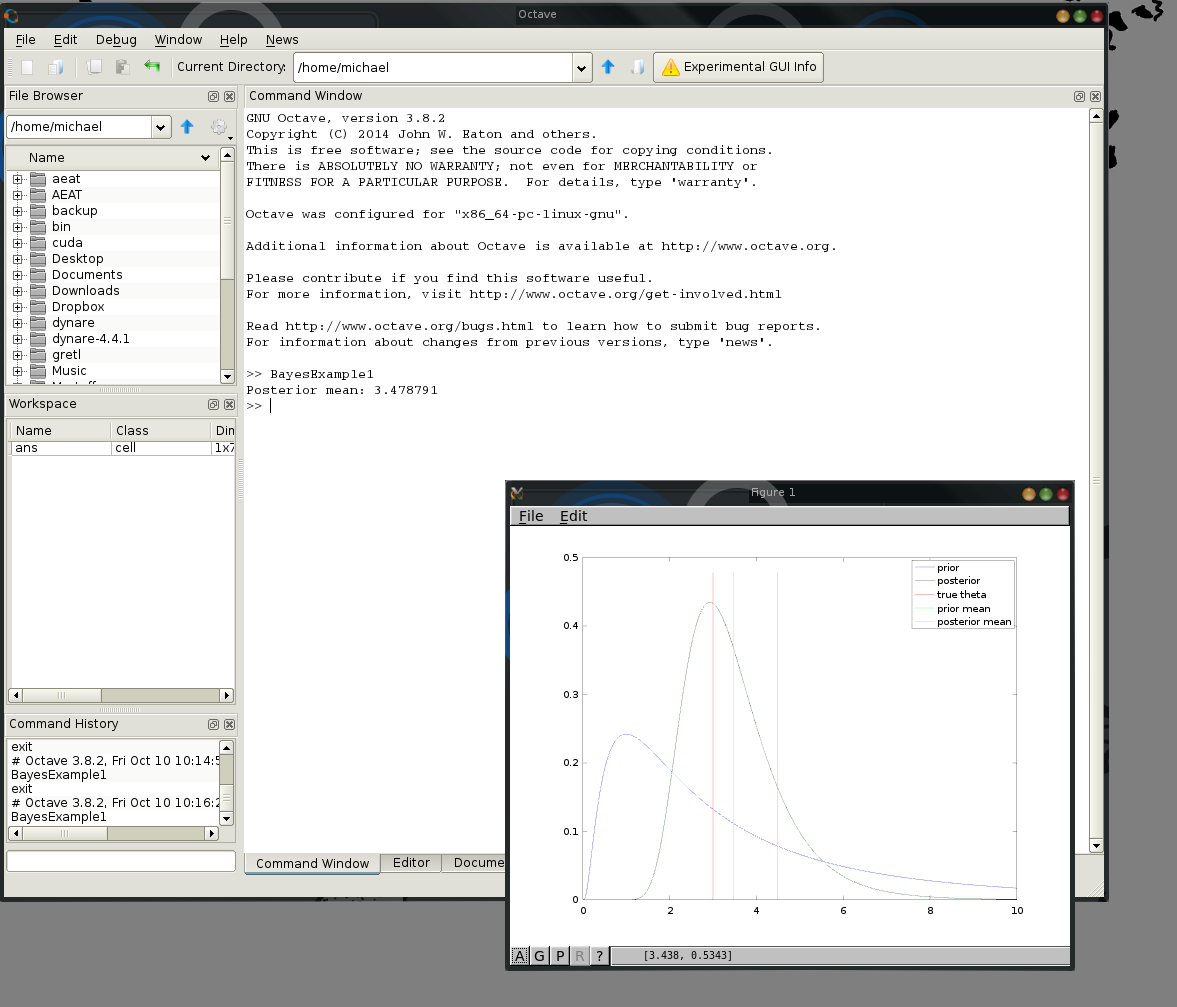
\includegraphics[width=4in]{Examples/Figures/octave}
\end{figure}
 As of 2011, some examples are being added using \htmladdnormallink{Gretl}{http://gretl.sourceforge.net}, the Gnu Regression, Econometrics, and Time-Series Library. This is an easy to use program, available in a number of languages, and it comes with a lot of data ready to use. It runs on the major operating systems. As of 2012, I am increasingly trying to make examples run on Matlab, though the need for add-on toolboxes for tasks as simple as generating random numbers limits what can be done. As of 2015, I will be adding examples using \htmladdnormallink{Julia}{http://julialang.org}, and in the long term, I plan to convert to using Julia as the main language. This is because Julia is friendly like Octave, but fast like C, it's free, and it runs on all the popular operating systems.

The main document was prepared using \LyX{} \htmladdnormallink{(www.lyx.org)}{http://www.lyx.org}. \LyX{} is a free\footnote{''Free'' is used in the sense of ''freedom'', but \LyX{} is also free of charge (free as in ''free beer'').} ``what you see is what you mean'' word processor, basically working as a graphical frontend to \LaTeX{}. It (with help from other applications) can export your work in \LaTeX{}, HTML, PDF and several other forms. It will run on Linux, Windows, and MacOS systems. Figure \ref{Picture of LyX} shows \LyX{} editing this document. 
\begin{figure}
\caption{\label{Picture of LyX}\protect\LyX{}}


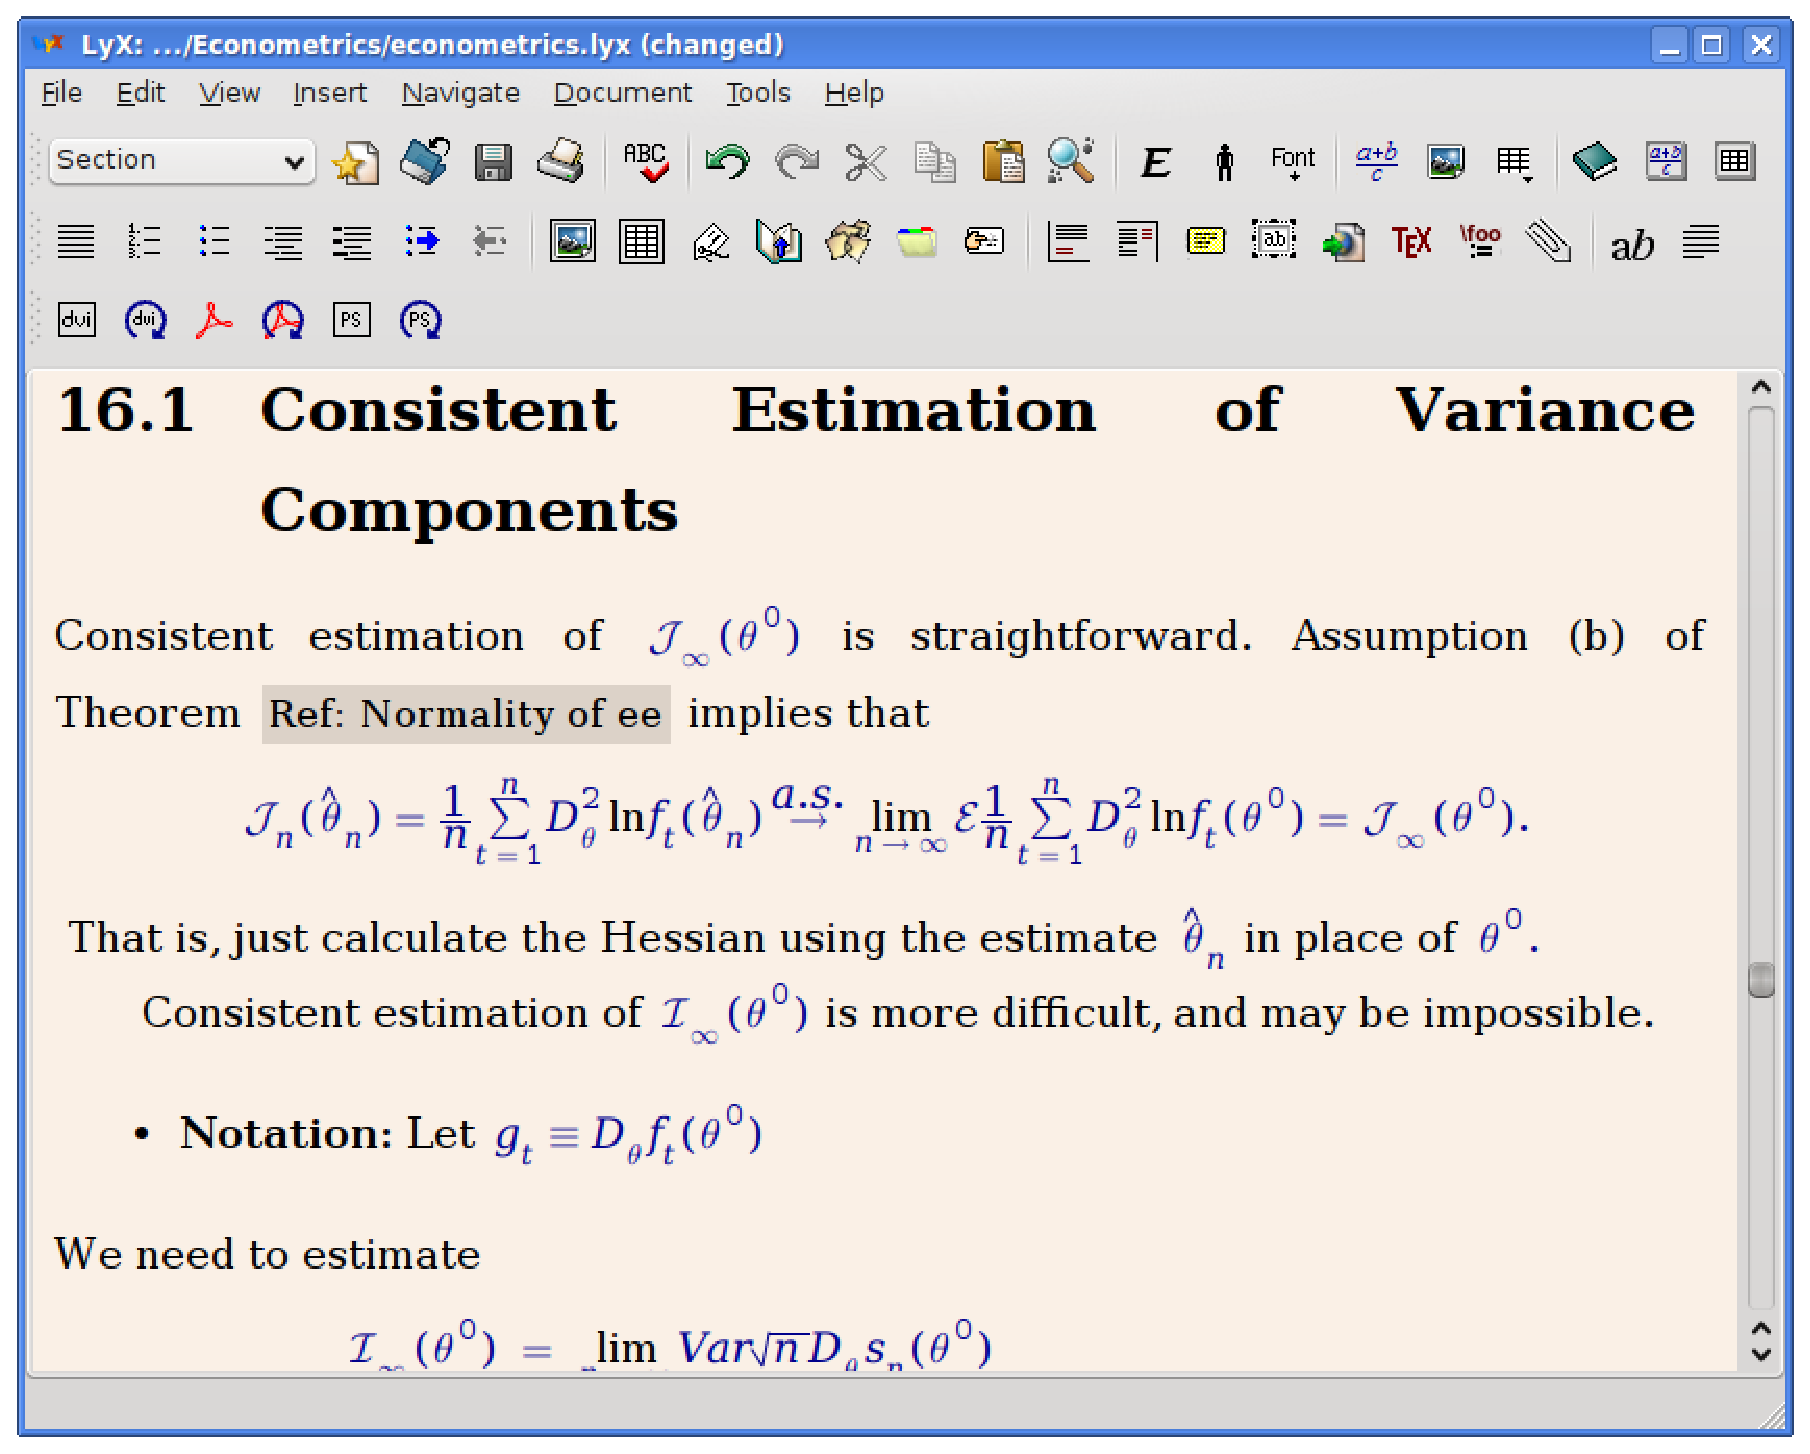
\includegraphics[width=6in]{Examples/Figures/lyx}
\end{figure}



\section{Licenses}

All materials are copyrighted by Michael Creel with the date that appears above. They are provided under the terms of the GNU General Public License, ver. 2, which forms Section \ref{GPL} of the notes, or, at your option, under the \htmladdnormallink{Creative Commons Attribution-Share Alike 2.5 license}{http://creativecommons.org/licenses/by-sa/2.5/}, which forms Section \ref{sec:Creative-Commons} of the notes. The main thing you need to know is that you are free to modify and distribute these materials in any way you like, as long as you share your contributions in the same way the materials are made available to you. In particular, you must make available the source files, in editable form, for your modified version of the materials. 


\section{Obtaining the materials}

The materials are available from a \href{https://github.com/mcreel/Econometrics/blob/master/}{github repository}. In addition to the final product, which you're probably looking at in some form now, you can obtain the editable \LyX{} sources, which will allow you to create your own version, if you like, or send error corrections and contributions. 


\section{\label{sec:BootableCD}econometrics.iso: An easy way run the examples}

Octave is available from the Octave home page, www.octave.org. Also, some updated links to packages for Windows and MacOS are at http://www.dynare.org/download/octave. The example programs are available as links embedded in the PDF version, and at \htmladdnormallink{here}{file:///home/michael/Mystuff/Econometrics/Examples}. Support files needed to run these are available \htmladdnormallink{here}{file:///home/michael/Mystuff/Econometrics/MyOctaveFiles}. The files won't run properly from your browser, because they are Octave scripts - they are only illustrative when browsing. To actually run the code, you need to check out the files from the \htmladdnormallink{repository}{https://github.com/mcreel/Econometrics}. There's a button for getting a zip file, and there are other options for download, too. Then you need to install Octave, set Octave's path, etc. All of this may sound a bit complicated, because it is (a bit). An easier solution is available: The \htmladdnormallink{econometrics.iso}{http://pareto.uab.cat/mcreel/econometrics.iso} file is an ISO image file. To download it from the repo, click on it, and then R-click on the RAW button, and select ''save as''. By default, this file will not be downloaded if you check out the repository, because it is about 1.5GB in size. It contains a bootable-from-CD or USB GNU/Linux system. These notes, in source form and as a PDF, together with all of the examples and the software needed to run them are available on econometrics.iso. I recommend starting off by using virtualization, to run the Linux system with all of the materials inside of a virtual computer, while still running your normal operating system. Various virtualization platforms are available. 
\begin{itemize}
\item I recommend \href{http://www.virtualbox.org/}{Virtualbox} \footnote{Virtualbox is free software (GPL v2). That, and the fact that it works very well, is the reason it is recommended here. There are a number of similar products available. It is possible to run PelicanHPC as a virtual machine, and to communicate with the installed operating system using a private network. Learning how to do this is not too difficult, and it is very convenient.}, which runs on Windows, Linux, and Mac OS.
\item If you use Virtualbox, you can import the appliance \htmladdnormallink{econometrics.ova }{file:///home/michael/Mystuff/Econometrics/econometrics.ova} using Virtualbox. 
\item Then the only remaing step is to adjust Settings/Storage to make the IDE controller point to the location where you have saved the econometrics.iso file. 
\item When you boot for the first time, append the boot parameter ''keyboard-layouts=es'', without quotes, and changing ''es'' to whatever code is appropriate for your keyboard. This may be tricky, as your keyboard layout won't be recognized until you do this.
\item Once you have it running, you can save the state of the virtual machine at any time, so that it will start up quickly, as you left it.
\item Once you have tried out the code, you may decide to check out the repo and install Octave on your actual physical computer. Running it with virtualization allows you to try it before you decide to take this step.
\end{itemize}
Figure \ref{fig:econometrics.iso-running-in} shows a screenshot of econometrics.iso running under Virtualbox. The GUI version of Octave is running a simple example of the delta method, while an instance of the command line interface is performing Bayesian MCMC estimation of a simple RBC model, using Dynare. You can access all of this without installing any software other that a virtualization platform, and using it to boot the econometrics.iso image.

\begin{figure}
\caption{\label{fig:econometrics.iso-running-in}econometrics.iso running in Virtualbox}


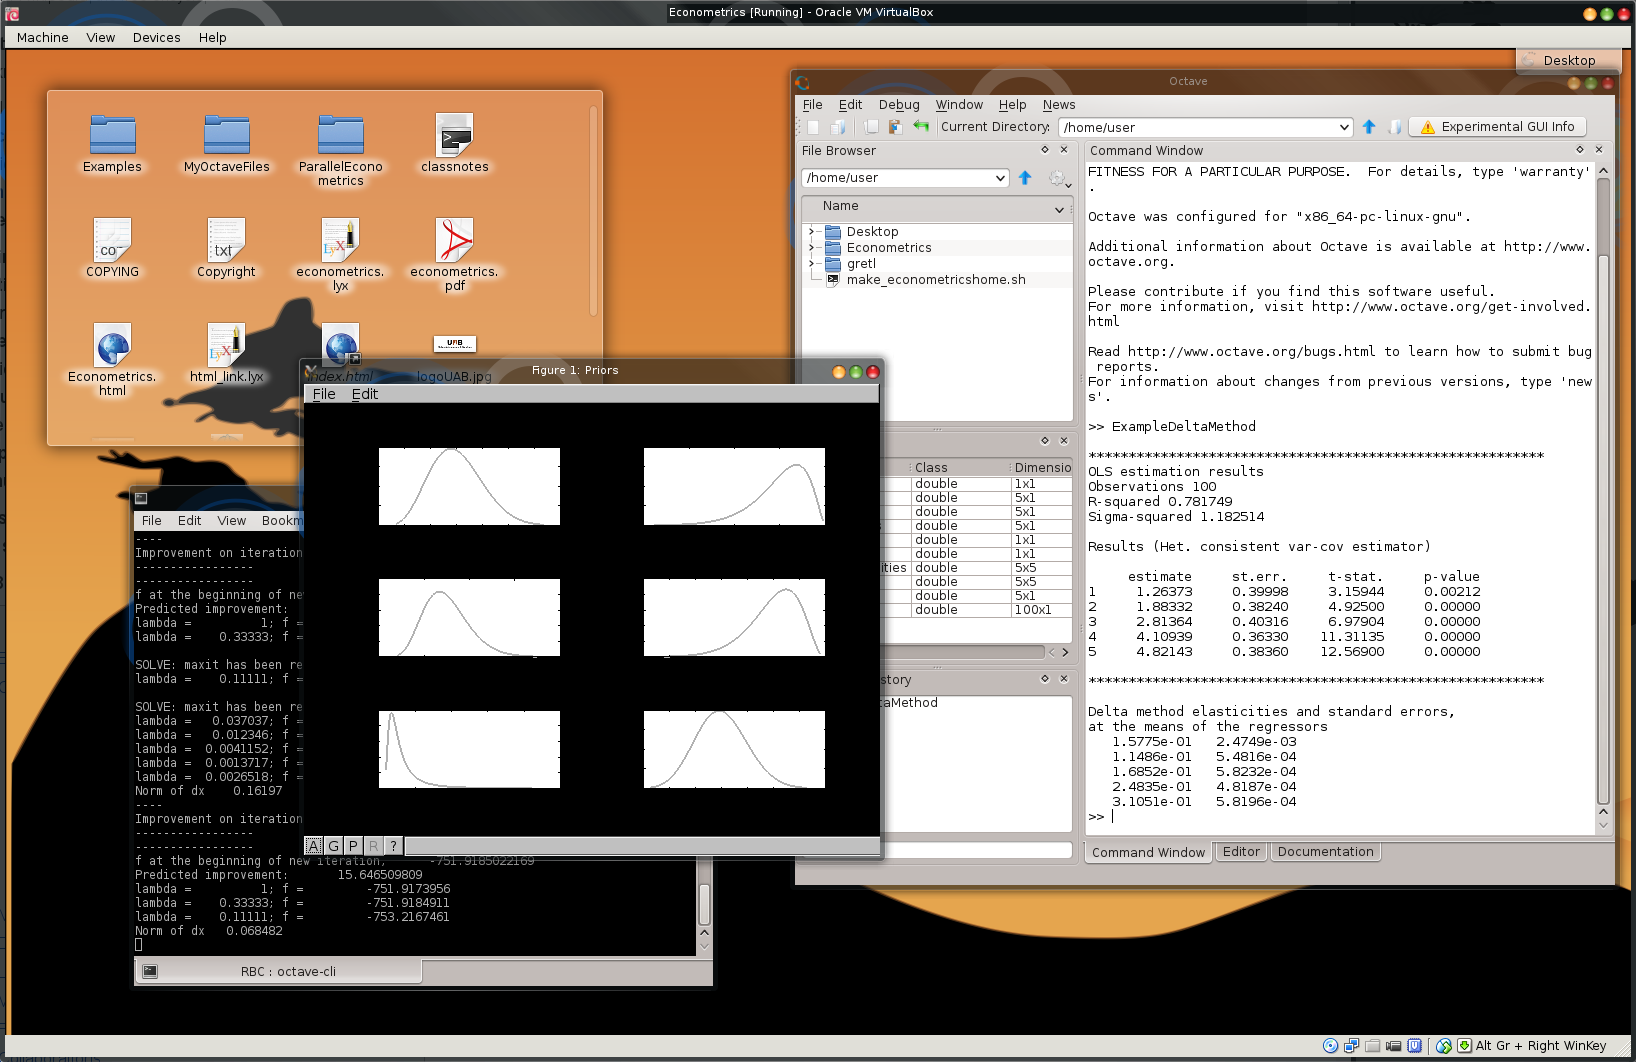
\includegraphics[width=4in]{EconometricsISO}
\end{figure}



\chapter{Introduction: Economic and econometric models}

Here's some  \htmladdnormallink{data}{file:///home/michael/Mystuff/Econometrics/Examples/Intro/data}: 100 observations on 3 economic variables. Let's do some exploratory analysis using Gretl:
\begin{itemize}
\item histograms
\item correlations
\item x-y scatterplots
\end{itemize}
So, what can we say? Correlations? Yes. Causality? Who knows? This is economic data, generated by economic agents, following their own beliefs, technologies and preferences. It is not experimental data generated under controlled conditions. How can we determine causality if we don't have experimental data? \newpage{}

Without a model, we can't distinguish correlation from causality. It turns out that the variables we're looking at are QUANTITY (q), PRICE (p), and INCOME (m). Economic theory tells us that the quantity of a good that consumers will puchase (the demand function) is something like: 
\[
q=f(p,m,z)
\]

\begin{itemize}
\item $q$ is the quantity demanded
\item $p$ is the price of the good
\item $m$ is income
\item $z$ is a vector of other variables that may affect demand
\end{itemize}
The supply of the good to the market is the aggregation of the firms' supply functions. The market supply function is something like
\[
q=g(p,z)
\]
Suppose we have a sample consisting of a number of observations on $q$ $p$ and $m$ at different time periods $t=1,2,...,n$. Supply and demand in each period is
\begin{align*}
q_{t} & =f(p_{t},m_{t},z_{t})\\
q_{t} & =g(p_{t},z_{t})
\end{align*}


\textbf{(draw some graphs showing roles of $m$ and $z$)}

This is the basic economic model of supply and demand: $q$ and $p$ are determined in the market equilibrium, given by the intersection of the two curves. These two variables are determined jointly by the model, and are the \emph{endogenous variables}. Income (m) is not determined by this model, its value is determined independently of q and p by some other process. m is an \emph{exogenous variable}. So, m causes q, though the demand function. Because q and p are jointly determined, m also causes p. p and q do not cause m, according to this theoretical model. q and p have a joint causal relationship.
\begin{itemize}
\item Economic theory can help us to determine the causality relationships between correlated variables.
\item If we had experimental data, we could control certain variables and observe the outcomes for other variables. If we see that variable $x$ changes as the controlled value of variable $y$ is changed, then we know that $y$ causes $x$. With economic data, we are unable to control the values of the variables: for example in supply and demand, if price changes, then quantity changes, but quantity also affect price. We can't control the market price, because the market price changes as quantity adjusts. This is the reason we need a theoretical model to help us distinguish correlation and causality.
\end{itemize}
The model is essentially a theoretical construct up to now:
\begin{itemize}
\item We don't know the forms of the functions $f$ and $g.$
\item Some components of $z_{t}$ may not be observable. For example, people don't eat the same lunch every day, and you can't tell what they will order just by looking at them. There are unobservable components to supply and demand, and we can model them as random variables. Suppose we can break $z_{t}$ into two unobservable components $\varepsilon_{t1}$ and $\epsilon_{t2}$.
\end{itemize}
An econometric model attempts to quantify the relationship more precisely. A step toward an estimable econometric model is to suppose that the model may be written as
\begin{align*}
q_{t} & =\alpha_{1}+\alpha_{2}p_{t}+\alpha_{3}m_{t}+\varepsilon_{t1}\\
q_{t} & =\beta_{1}+\beta_{2}p_{t}+\varepsilon_{t1}
\end{align*}
 We have imposed a number of restrictions on the theoretical model:
\begin{itemize}
\item The functions $f$ and $g$ have been specified to be linear functions
\item The parameters ($\alpha_{1},$ $\beta_{2},$ etc.) are constant over time.
\item There is a single unobservable component in each equation, and we assume it is additive.
\end{itemize}
If we assume nothing about the error terms $\epsilon_{t1}$ and $\epsilon_{t2}$, we can always write the last two equations, as the errors simply make up the difference between the true demand and supply functions and the assumed forms. But in order for the $\beta$ coefficients to exist in a sense that has economic meaning, and in order to be able to use sample data to make reliable inferences about their values, we need to make additional assumptions. Such assumptions might be something like:
\begin{itemize}
\item $E(\epsilon_{tj})=0,\,j=1,2$
\item $E(p_{t}\epsilon_{tj})=0,\,j=1,2$
\item $E(m_{t}\epsilon_{tj})=0,\,j=1,2$
\end{itemize}
These are assertions that the errors are uncorrelated with the variables, and such assertions may or may not be reasonable. Later we will see how such assumption may be used and/or tested.

All of the last six bulleted points have \textbf{no theoretical basis}, in that the theory of supply and demand doesn't imply these conditions. The validity of any results we obtain using this model will be contingent on these additional restrictions being at least approximately correct. For this reason, \emph{specification testing} will be needed, to check that the model seems to be reasonable. Only when we are convinced that the model is at least approximately correct should we use it for economic analysis. 

When testing a hypothesis using an econometric model, at least three factors can cause a statistical test to reject the null hypothesis:
\begin{enumerate}
\item the hypothesis is false
\item a type I error has occured
\item the econometric model is not correctly specified, and thus the test does not have the assumed distribution
\end{enumerate}
To be able to make scientific progress, we would like to ensure that the third reason is not contributing in a major way to rejections, so that rejection will be most likely due to either the first or second reasons. Hopefully the above example makes it clear that econometric models are necessarily more detailed than what we can obtain from economic theory, and that this additional detail introduces many possible sources of misspecification of econometric models. In the next few sections we will obtain results supposing that the econometric model is entirely correctly specified. Later we will examine the consequences of misspecification and see some methods for determining if a model is correctly specified. Later on, econometric methods that seek to minimize maintained assumptions are introduced.

\newpage


\chapter{Ordinary Least Squares}


\section{The Linear Model}

Consider approximating a variable $y$ using the variables $x_{1},x_{2},...,x_{k}$. We can consider a model that is a linear approximation:

\textbf{Linearity}: the model is a linear function of the parameter vector $\beta^{0}:$
\begin{eqnarray*}
y & = & \beta_{1}^{0}x_{1}+\beta_{2}^{0}x_{2}+...+\beta_{k}^{0}x_{k}+\epsilon
\end{eqnarray*}
or, using vector notation: 
\[
y=\mathbf{x}^{\prime}\beta^{0}+\epsilon
\]
 The dependent variable $y$ is a scalar random variable, $\mathbf{x}=(\begin{array}{cccc}
x_{1} & x_{2} & \cdots & x_{k})^{'}\end{array}$ is a $k$-vector of explanatory variables, and $\beta^{0}=(\begin{array}{cccc}
\beta_{1}^{0} & \beta_{2}^{0} & \cdots & \beta_{k}^{0})^{'}\end{array}.$ The superscript ``0'' in $\beta^{0}$ means this is the ''true value'' of the unknown parameter. It will be defined more precisely later, and usually suppressed when it's not necessary for clarity. 

Suppose that we want to use data to try to determine the best linear approximation to $y$ using the variables $\mathbf{x}.$ The data $\left\{ (y_{t},\mathbf{x}_{t})\right\} ,t=1,2,...,n$ are obtained by some form of sampling\footnote{For example, cross-sectional data may be obtained by random sampling. Time series data accumulate historically.}. An individual observation is
\[
y_{t}=\mathbf{x}_{t}^{\prime}\beta+\varepsilon_{t}
\]
 The $n$ observations can be written in matrix form as 
\begin{equation}
\mathbf{y}=\mathbf{X}\beta+\mathbf{\varepsilon},
\end{equation}
 where $\mathbf{y}=\left(\begin{array}{cccc}
y_{1} & y_{2} & \cdots & y_{n}\end{array}\right)^{\prime}$ is $n\times1$ and $\mathbf{X}=\left(\begin{array}{cccc}
\mathbf{x}_{1} & \mathbf{x}_{2} & \cdots & \mathbf{x}_{n}\end{array}\right)^{\prime}$.

Linear models are more general than they might first appear, since one can employ nonlinear transformations of the variables: 
\[
\varphi_{0}(z)=\left[\begin{array}{cccc}
\varphi_{1}(w) & \varphi_{2}(w) & \cdots & \varphi_{p}(w)\end{array}\right]\beta+\varepsilon
\]
 where the $\phi_{i}()$ are known functions. Defining $y=\varphi_{0}(z),$ $x_{1}=\varphi_{1}(w),$ \emph{etc}. leads to a model in the form of equation \ref{assumption: linearity}. For example, the Cobb-Douglas model\index{Cobb-Douglas model} 
\[
z=Aw_{2}^{\beta_{2}}w_{3}^{\beta_{3}}\exp(\varepsilon)
\]
 can be transformed logarithmically to obtain 
\[
\ln z=\ln A+\beta_{2}\ln w_{2}+\beta_{3}\ln w_{3}+\varepsilon.
\]
If we define $y=\ln z,$ $\beta_{1}=\ln A,$ \emph{etc.,} we can put the model in the form needed. The approximation is linear in the parameters, but not necessarily linear in the variables.


\section{Estimation by least squares}

Figure \ref{cap:Typical-data,-Classical}, obtained by running  \htmladdnormallink{TypicalData.m}{file:///home/michael/Mystuff/Econometrics/Examples/OLS/TypicalData.m} shows some data that follows the linear model $y_{t}=\beta_{1}+\beta_{2}x_{t2}+\epsilon_{t}$. The green line is the ''true'' regression line $\beta_{1}+\beta_{2}x_{t2}$, and the red crosses are the data points $(x_{t2},y_{t}),$ where $\epsilon_{t}$ is a random error that has mean zero and is independent of $x_{t2}$. Exactly how the green line is defined will become clear later. In practice, we only have the data, and we don't know where the green line lies. We need to gain information about the straight line that best fits the data points. 
\begin{figure}
\caption{\label{cap:Typical-data,-Classical}Typical data, Classical Model}


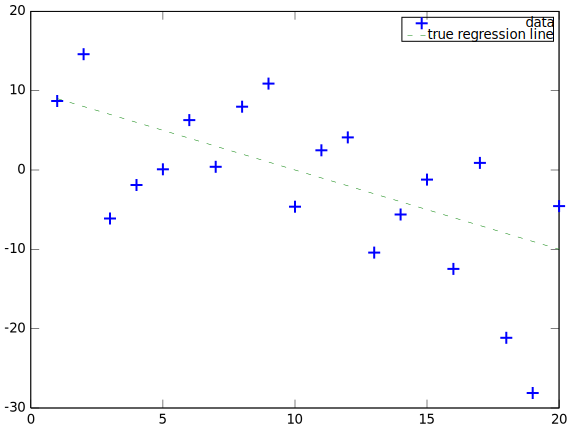
\includegraphics{Examples/OLS/TypicalData}
\end{figure}


The \emph{ordinary least squares} (OLS) estimator is defined as the value that minimizes the sum of the squared errors: 
\begin{eqnarray*}
\hat{\beta} & = & \arg\min s(\beta)
\end{eqnarray*}
 where

\begin{eqnarray}
s(\beta) & = & \sum_{t=1}^{n}\left(y_{t}-\mathbf{x}_{t}^{\prime}\beta\right)^{2}\label{eq:OLS criterion function}\\
 & = & \left(\mathbf{y}-\mathbf{X}\beta\right)^{\prime}\left(\mathbf{y}-\mathbf{X}\beta\right)\nonumber \\
 & = & \mathbf{y}^{\prime}\mathbf{y}-2\mathbf{y}^{\prime}\mathbf{X}\beta+\beta^{\prime}\mathbf{X}^{\prime}\mathbf{X}\beta\nonumber \\
 & = & \parallel\mathbf{y}-\mathbf{X}\beta\parallel^{2}\nonumber 
\end{eqnarray}
This last expression makes it clear how the OLS estimator\index{estimator, OLS} is defined: it minimizes the Euclidean distance between $y$ and $X\beta.$ The fitted OLS coefficients are those that give the best linear approximation to $y$ using $\mathbf{x}$ as basis functions, where ''best'' means minimum Euclidean distance. One could think of other estimators based upon other metrics. For example, the \emph{minimum absolute distance} (MAD) minimizes $\sum_{t=1}^{n}\left|y_{t}-\mathbf{x}_{t}^{\prime}\beta\right|$. Later, we will see that which estimator is best in terms of their statistical properties, rather than in terms of the metrics that define them, depends upon the properties of $\epsilon$, about which we have as yet made no assumptions.
\begin{itemize}
\item To minimize the criterion $s(\beta),$ find the derivative with respect to $\beta$: 
\begin{eqnarray*}
D_{\beta}s(\beta) & = & -2\mathbf{X}^{\prime}\mathbf{y}+2\mathbf{X}^{\prime}\mathbf{X}\beta
\end{eqnarray*}
Then setting it to zeros gives
\[
D_{\beta}s(\hat{\beta})=-2\mathbf{X}^{\prime}\mathbf{y}+2\mathbf{X}^{\prime}\mathbf{X}\hat{\beta}\equiv0
\]
 so
\[
\hat{\beta}=(\mathbf{X}^{\prime}\mathbf{X})^{-1}\mathbf{X}^{\prime}\mathbf{y}.
\]

\item To verify that this is a minimum, check the second order sufficient condition: 
\[
D_{\beta}^{2}s(\hat{\beta})=2\mathbf{X}^{\prime}\mathbf{X}
\]
 Since $\rho(\mathbf{X})=K,$ this matrix is positive definite, since it's a quadratic form in a p.d. matrix (identity matrix of order $n)$, so $\hat{\beta}$ is in fact a minimizer.
\item The \emph{fitted values\index{fitted values}} are the vector $\hat{\mathbf{y}}=\mathbf{X}\hat{\beta}.$
\item The \emph{residuals\index{residuals}} are the vector $\hat{\varepsilon}=\mathbf{y}-\mathbf{X}\hat{\beta}$
\item Note that 
\begin{eqnarray*}
\mathbf{y} & = & \mathbf{X}\beta+\varepsilon\\
 & = & \mathbf{X}\hat{\beta}+\hat{\varepsilon}
\end{eqnarray*}

\item Also, the first order conditions can be written as 
\begin{eqnarray*}
\mathbf{X}^{\prime}\mathbf{y}-\mathbf{X}^{\prime}\mathbf{X}\hat{\beta} & = & 0\\
\mathbf{X}^{\prime}\left(\mathbf{y}-\mathbf{X}\hat{\beta}\right) & = & 0\\
\mathbf{X}^{\prime}\hat{\varepsilon} & = & 0
\end{eqnarray*}
which is to say, the OLS residuals are orthogonal to $\mathbf{X}$. Let's look at this more carefully.
\end{itemize}

\section{Geometric interpretation of least squares estimation}


\subsection{In $X,Y$ Space}

Figure \ref{fitted in X,Y space} shows a typical fit to data, along with the true regression line. Note that the true line and the estimated line are different. This figure was created by running the Octave program  \htmladdnormallink{OlsFit.m}{file:///home/michael/Mystuff/Econometrics/Examples/OLS/OlsFit.m} . You can experiment with changing the parameter values to see how this affects the fit, and to see how the fitted line will sometimes be close to the true line, and sometimes rather far away. 
\begin{figure}
\caption{\label{fitted in X,Y space}Example OLS Fit}


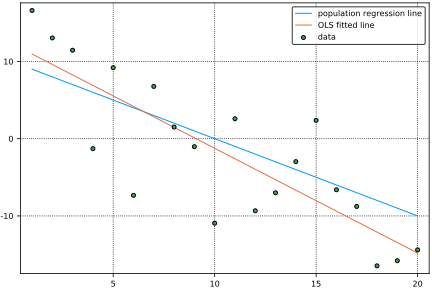
\includegraphics{Examples/OLS/OlsFit}
\end{figure}



\subsection{In Observation Space}

If we want to plot in observation space, we'll need to use only two or three observations, or we'll encounter some limitations of the blackboard. If we try to use 3, we'll encounter the limits of my artistic ability, so let's use two. With only two observations, we can't have $K>1.$ 
\begin{figure}[htbp]
\caption{The fit in observation space}


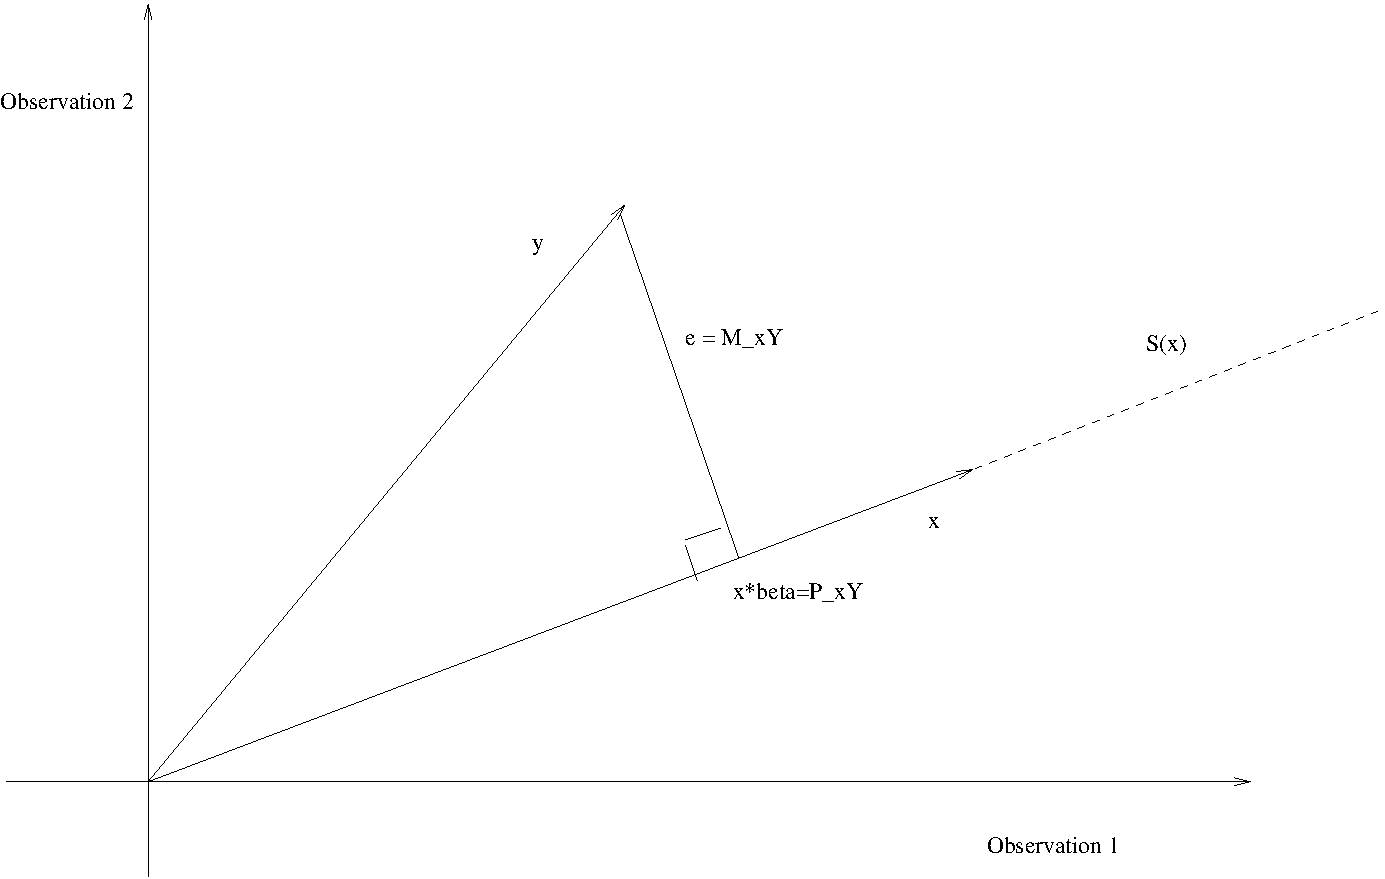
\includegraphics[width=6in]{Examples/Figures/regression_obs_space}
\end{figure}
 
\begin{itemize}
\item We can decompose $y$ into two components: the orthogonal projection onto the $K-$dimensional space spanned by $X$, $X\hat{\beta},$ and the component that is the orthogonal projection onto the $n-K$ subpace that is orthogonal to the span of $X,$ $\hat{\varepsilon}.$
\item Since $\hat{\beta}$ is chosen to make $\hat{\varepsilon}$ as short as possible, $\hat{\varepsilon}$ will be orthogonal to the space spanned by $X.$ Since $X$ is in this space, $X^{\prime}\hat{\varepsilon}=0.$ Note that the f.o.c. that define the least squares estimator imply that this is so.
\end{itemize}

\subsection{Projection Matrices}

$X\hat{\beta}$ is the projection of $y$ onto the span of $X,$ or 
\[
X\hat{\beta}=X\left(X^{\prime}X\right)^{-1}X^{\prime}y
\]
 Therefore, the matrix\index{matrix, projection} that projects $y$ onto the span of $X$ is 
\[
P_{X}=X(X^{\prime}X)^{-1}X^{\prime}
\]
 since 
\[
X\hat{\beta}=P_{X}y.
\]
$\hat{\varepsilon}$ is the projection of $y$ onto the $N-K$ dimensional space that is orthogonal to the span of $X$. We have that 
\begin{eqnarray*}
\hat{\varepsilon} & = & y-X\hat{\beta}\\
 & = & y-X(X^{\prime}X)^{-1}X^{\prime}y\\
 & = & \left[I_{n}-X(X^{\prime}X)^{-1}X^{\prime}\right]y.
\end{eqnarray*}
 So the matrix that projects $y$ onto the space orthogonal to the span of $X$ is 
\begin{eqnarray*}
M_{X} & = & I_{n}-X(X^{\prime}X)^{-1}X^{\prime}\\
 & = & I_{n}-P_{X}.
\end{eqnarray*}
 We have 
\[
\hat{\varepsilon}=M_{X}y.
\]
Therefore 
\begin{eqnarray*}
y & = & P_{X}y+M_{X}y\\
 & = & X\hat{\beta}+\hat{\varepsilon}.
\end{eqnarray*}
These two projection matrices decompose the $n$ dimensional vector $y$ into two orthogonal components - the portion that lies in the $K$ dimensional space defined by $X,$ and the portion that lies in the orthogonal $n-K$ dimensional space.
\begin{itemize}
\item Note that both $P_{X}$ and $M_{X}$ are \emph{symmetric} and \emph{idempotent}.

\begin{itemize}
\item A symmetric matrix\index{matrix, symmetric} $A$ is one such that $A=A^{\prime}.$
\item An idempotent matrix\index{matrix, idempotent} $A$ is one such that $A=AA.$
\item The only nonsingular idempotent matrix is the identity matrix. 
\end{itemize}
\end{itemize}

\section{Influential observations\index{observations, influential} and outliers\index{outliers}}

The OLS estimator of the $i^{th}$ element of the vector $\beta_{0}$ is simply 
\begin{eqnarray*}
\hat{\beta}_{i} & = & \left[(X^{\prime}X)^{-1}X^{\prime}\right]_{i\cdot}y\\
 & = & c_{i}^{\prime}y
\end{eqnarray*}


This is how we define a linear estimator\index{estimator, linear} - it's a linear function of the dependent variable. Since it's a linear combination of the observations on the dependent variable, where the weights are determined by the observations on the regressors, some observations may have more influence than others.

To investigate this, let $e_{t}$ be an $n$ vector of zeros with a $1$ in the t$^{th}$ position, \emph{i.e.,} it's the $t\textrm{th column of the matrix \ensuremath{I_{n}}}$. Define 
\begin{eqnarray*}
h_{t} & = & \left(P_{X}\right)_{tt}\\
 & = & e_{t}^{\prime}P_{X}e_{t}
\end{eqnarray*}
 so $h_{t}$ is the t$^{th}$ element on the main diagonal of $P_{X}$. Note that 
\begin{eqnarray*}
h_{t} & = & \parallel P_{X}e_{t}\parallel^{2}
\end{eqnarray*}
so 
\[
h_{t}\leq\parallel e_{t}\parallel^{2}=1
\]
So $0<h_{t}<1$. Also, 
\[
TrP_{X}=K\Rightarrow\overline{h}=K/n.
\]
So the average of the $h_{t}$ is $K/n$. The value $h_{t}$ is referred to as the \emph{leverage\index{leverage}} of the observation. If the leverage is much higher than average, the observation has the potential to affect the OLS fit importantly. However, an observation may also be influential due to the value of $y_{t}$, rather than the weight it is multiplied by, which only depends on the $x_{t}$'s.

To account for this, consider estimation of $\beta$ without using the $t^{th}$ observation (designate this estimator as $\hat{\beta}^{(t)}).$ One can show (see Davidson and MacKinnon, pp. 32-5 for proof) that 
\[
\hat{\beta}^{(t)}=\hat{\beta}-\left(\frac{1}{1-h_{t}}\right)(X^{\prime}X)^{-1}X_{t}^{\prime}\hat{\varepsilon}_{t}
\]
 so the change in the $t^{th}$ observations fitted value is 
\[
\mathbf{x}_{t}^{\prime}\hat{\beta}-\mathbf{x}_{t}^{\prime}\hat{\beta}^{(t)}=\left(\frac{h_{t}}{1-h_{t}}\right)\hat{\varepsilon}_{t}
\]
 While an observation may be influential if it doesn't affect its own fitted value, it certainly \emph{is} influential if it does. A fast means of identifying influential observations is to plot $\left(\frac{h_{t}}{1-h_{t}}\right)\hat{\varepsilon}_{t}$ (which I will refer to as the \emph{own influence\index{own influence}} of the observation) as a function of $t$. Figure \ref{cap:Detection-of-influential} gives an example plot of data, fit, leverage and influence. The Octave program is  \htmladdnormallink{InfluentialObservation.m}{file:///home/michael/Mystuff/Econometrics/Examples/OLS/InfluentialObservation.m}. \textbf{(note to self when lecturing: load the data ../OLS/influencedata into Gretl and reproduce this).} If you re-run the program you will see that the leverage of the last observation (an outlying value of x) is always high, and the influence is sometimes high.

\begin{figure}
\caption{\label{cap:Detection-of-influential}Detection of influential observations}


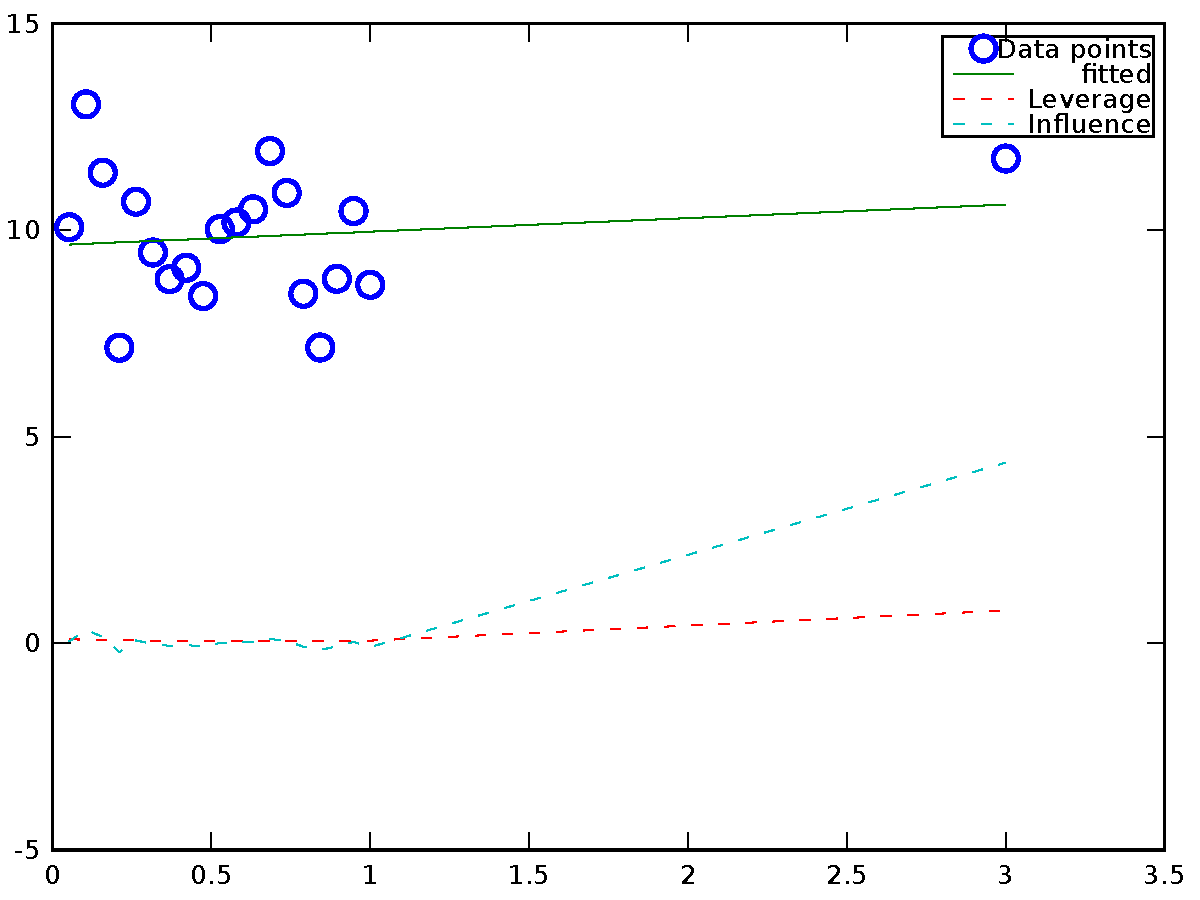
\includegraphics{Examples/OLS/InfluentialObservation}
\end{figure}


After influential observations are detected, one needs to determine \emph{why} they are influential. Possible causes include:
\begin{itemize}
\item data entry error, which can easily be corrected once detected. Data entry errors \emph{are very common.}
\item special economic factors that affect some observations. These would need to be identified and incorporated in the model. This is the idea behind \emph{structural change}: the parameters may not be constant across all observations.
\item pure randomness may have caused us to sample a low-probability observation.
\end{itemize}
There exist \emph{robust} estimation methods that downweight outliers.


\section{Goodness of fit}

The fitted model is 
\[
y=X\hat{\beta}+\hat{\varepsilon}
\]
 Take the inner product:

\[
y^{\prime}y=\hat{\beta}^{\prime}X^{\prime}X\hat{\beta}+2\hat{\beta}^{\prime}X^{\prime}\hat{\varepsilon}+\hat{\varepsilon}^{\prime}\hat{\varepsilon}
\]
 But the middle term of the RHS is zero since $X^{\prime}\hat{\varepsilon}=0$, so 
\begin{equation}
y^{\prime}y=\hat{\beta}^{\prime}X^{\prime}X\hat{\beta}+\hat{\varepsilon}^{\prime}\hat{\varepsilon}\label{rsquare development}
\end{equation}
 The \emph{uncentered} $R_{u}^{2}$ is defined as 
\begin{eqnarray*}
R_{u}^{2} & = & 1-\frac{\hat{\varepsilon}^{\prime}\hat{\varepsilon}}{y^{\prime}y}\\
 & = & \frac{\hat{\beta}^{\prime}X^{\prime}X\hat{\beta}}{y^{\prime}y}\\
 & = & \frac{\parallel P_{X}y\parallel^{2}}{\parallel y\parallel^{2}}\\
 & = & \cos^{2}(\phi),
\end{eqnarray*}
 where $\phi$ is the angle between $y$ and the span of $X$ .
\begin{itemize}
\item The uncentered $R^{2}$\index{R- squared, uncentered} changes if we add a constant to $y,$ since this changes $\phi$ (see Figure \ref{Uncentered--R^=00007B2=00007D}, the yellow vector is a constant, since it's on the $45$ degree line in observation space). 
\begin{figure}[htbp]
\caption{\label{Uncentered--R^=00007B2=00007D}Uncentered $R^{2}$}


\centering{}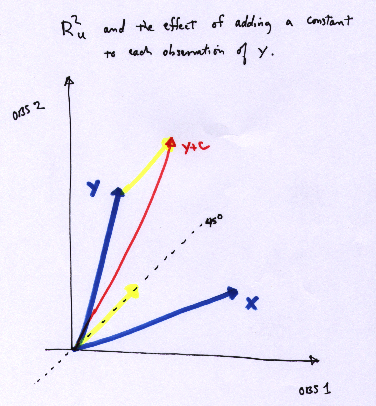
\includegraphics[width=5in,height=4in]{/home/michael/Mystuff/Econometrics/Examples/Figures/UncenteredRSquare}
\end{figure}
Another, more common definition measures the contribution of the variables, other than the constant term, to explaining the variation in $y.$ Thus it measures the ability of the model to explain the variation of $y$ about its unconditional sample mean.
\end{itemize}
Let $\iota=(1,1,...,1)^{\prime},$ a $n$ -vector. So 
\begin{eqnarray*}
M_{\iota} & = & I_{n}-\iota(\iota^{\prime}\iota)^{-1}\iota^{\prime}\\
 & = & I_{n}-\iota\iota^{\prime}/n
\end{eqnarray*}
 $M_{\iota}y$ just returns the vector of deviations from the mean. In terms of deviations from the mean, equation \ref{rsquare development} becomes
\[
y^{\prime}M_{\iota}y=\hat{\beta}^{\prime}X^{\prime}M_{\iota}X\hat{\beta}+\hat{\varepsilon}^{\prime}M_{\iota}\hat{\varepsilon}
\]
 

The \emph{centered\index{R-squared, centered}} $R_{c}^{2}$ is defined as 
\[
R_{c}^{2}=1-\frac{\hat{\varepsilon}^{\prime}\hat{\varepsilon}}{y^{\prime}M_{\iota}y}=1-\frac{ESS}{TSS}
\]
where $ESS=\hat{\varepsilon}^{\prime}\hat{\varepsilon}$ and $TSS=y^{\prime}M_{\iota}y$=$\sum_{t=1}^{n}(y_{t}-\bar{y})^{2}$.

Supposing that $X$ contains a column of ones (\emph{i.e.,} there is a constant term), 
\[
X^{\prime}\hat{\varepsilon}=0\Rightarrow\sum_{t}\hat{\varepsilon}_{t}=0
\]
 so $M_{\iota}\hat{\varepsilon}$ $=\hat{\varepsilon}.$ In this case 
\[
y^{\prime}M_{\iota}y=\hat{\beta}^{\prime}X^{\prime}M_{\iota}X\hat{\beta}+\hat{\varepsilon}^{\prime}\hat{\varepsilon}
\]
 So 
\[
R_{c}^{2}=\frac{RSS}{TSS}
\]
where $RSS=\hat{\beta}^{\prime}X^{\prime}M_{\iota}X\hat{\beta}$ 
\begin{itemize}
\item Supposing that a column of ones is in the space spanned by $X$ ($P_{X}\iota=\iota),$ then one can show that $0\leq R_{c}^{2}\leq1.$
\end{itemize}

\section{The classical linear regression model\label{sec:The-classical-linear}}

Up to this point the model is empty of content beyond the definition of a best linear approximation to $y$ and some geometrical properties. There is no economic content to the model, and the regression parameters have no economic interpretation. For example, what is the partial derivative of $y$ with respect to $x_{j}$? The linear approximation is
\[
y=\beta_{1}x_{1}+\beta_{2}x_{2}+...+\beta_{k}x_{k}+\epsilon
\]
The partial derivative is 
\[
\frac{\partial y}{\partial x_{j}}=\beta_{j}+\frac{\partial\epsilon}{\partial x_{j}}
\]
Up to now, there's no guarantee that $\frac{\partial\epsilon}{\partial x_{j}}$=0. For the $\beta$ to have an economic meaning, we need to make additional assumptions. The assumptions that are appropriate to make depend on the data under consideration. We'll start with the classical linear regression model, which incorporates some assumptions that are clearly not realistic for economic data. This is to be able to explain some concepts with a minimum of confusion and notational clutter. Later we'll adapt the results to what we can get with more realistic assumptions.

\textbf{Linearity}: the model is a linear function of the parameter vector $\beta^{0}:$
\begin{eqnarray}
y & = & \beta_{1}^{0}x_{1}+\beta_{2}^{0}x_{2}+...+\beta_{k}^{0}x_{k}+\epsilon\label{assumption: linearity}
\end{eqnarray}
or, using vector notation: 
\[
y=\mathbf{x}^{\prime}\beta^{0}+\epsilon
\]


\textbf{Nonstochastic linearly independent regressors}: $\mathbf{X}$ is a fixed matrix of constants, it has rank $K$ equal to its number of columns, and 
\begin{align}
\lim\frac{1}{n}\mathbf{X}^{\prime}\mathbf{X} & =Q_{X}\label{assumption: linearly independent regressors}
\end{align}
where $Q_{X}$ is a finite positive definite matrix. This is needed to be able to identify the individual effects of the explanatory variables.

\textbf{Independently and identically distributed errors}:
\begin{equation}
\epsilon\sim IID(0,\sigma^{2}I_{n})\label{assumption: IID errors}
\end{equation}
$\varepsilon$ is jointly distributed IID. This implies the following two properties:

\textbf{Homoscedastic errors}:
\begin{equation}
V(\varepsilon_{t})=\sigma_{0}^{2},\forall t\label{assumption: homoscedasticity}
\end{equation}


\textbf{Nonautocorrelated errors:}

\begin{equation}
\mathcal{E}(\varepsilon_{t}\epsilon_{s})=0,\forall t\neq s\label{assumption: nonautocorrelation}
\end{equation}


Optionally, we will sometimes assume that the errors are normally distributed.

\textbf{Normally distributed errors:}
\begin{equation}
\epsilon\sim N(0,\sigma^{2}I_{n})\label{assumption: normal errors}
\end{equation}



\section{Small sample statistical properties of the least squares estimator}

Up to now, we have only examined numeric properties of the OLS estimator, that always hold. Now we will examine statistical properties. The statistical properties depend upon the assumptions we make.


\subsection{Unbiasedness}

We have $\hat{\beta}=(X^{\prime}X)^{-1}X^{\prime}y$. By linearity, 
\begin{eqnarray*}
\hat{\beta} & = & (X^{\prime}X)^{-1}X^{\prime}\left(X\beta+\varepsilon\right)\\
 & = & \beta+(X^{\prime}X)^{-1}X^{\prime}\varepsilon
\end{eqnarray*}
By \ref{assumption: linearly independent regressors} and \ref{assumption: IID errors}
\begin{eqnarray*}
E(X^{\prime}X)^{-1}X^{\prime}\varepsilon & = & E(X^{\prime}X)^{-1}X^{\prime}\varepsilon\\
 & = & (X^{\prime}X)^{-1}X^{\prime}E\varepsilon\\
 & = & 0
\end{eqnarray*}
 so the OLS estimator is unbiased under the assumptions of the classical model.

Figure \ref{figure-unbiasedness} shows the results of a small Monte Carlo experiment where the OLS estimator was calculated for 10000 samples from the classical model with $y=1+2x+\varepsilon$, where $n=20$, $\sigma_{\varepsilon}^{2}=9$, and $x$ is fixed across samples. We can see that the $\beta_{2}$ appears to be estimated without bias. The program that generates the plot is  \htmladdnormallink{Unbiased.m}{file:///home/michael/Mystuff/Econometrics/Examples/OLS/Unbiased.m} , if you would like to experiment with this.

\begin{figure}
\caption{\label{figure-unbiasedness}Unbiasedness of OLS under classical assumptions}


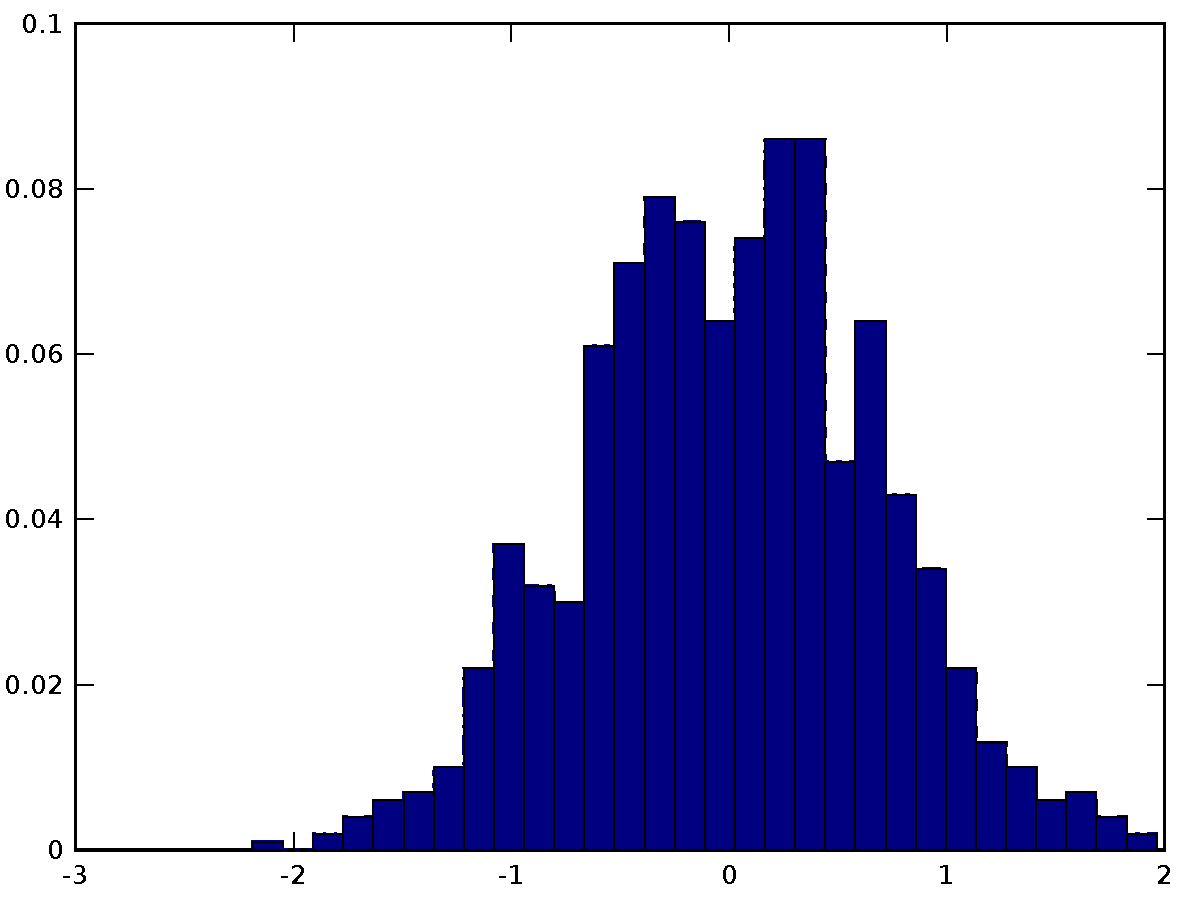
\includegraphics{Examples/OLS/Unbiased}
\end{figure}


With time series data, the OLS estimator will often be biased. Figure \ref{figure-biasedness} shows the results of a small Monte Carlo experiment where the OLS estimator was calculated for 1000 samples from the AR(1) model with $y_{t}=0+0.9y_{t-1}+\varepsilon_{t}$, where $n=20$ and $\sigma_{\varepsilon}^{2}=1$. In this case, assumption \ref{assumption: linearly independent regressors} does not hold: the regressors are stochastic. We can see that the bias in the estimation of $\beta_{2}$ is about -0.2.

\begin{figure}
\caption{\label{figure-biasedness}Biasedness of OLS when an assumption fails}


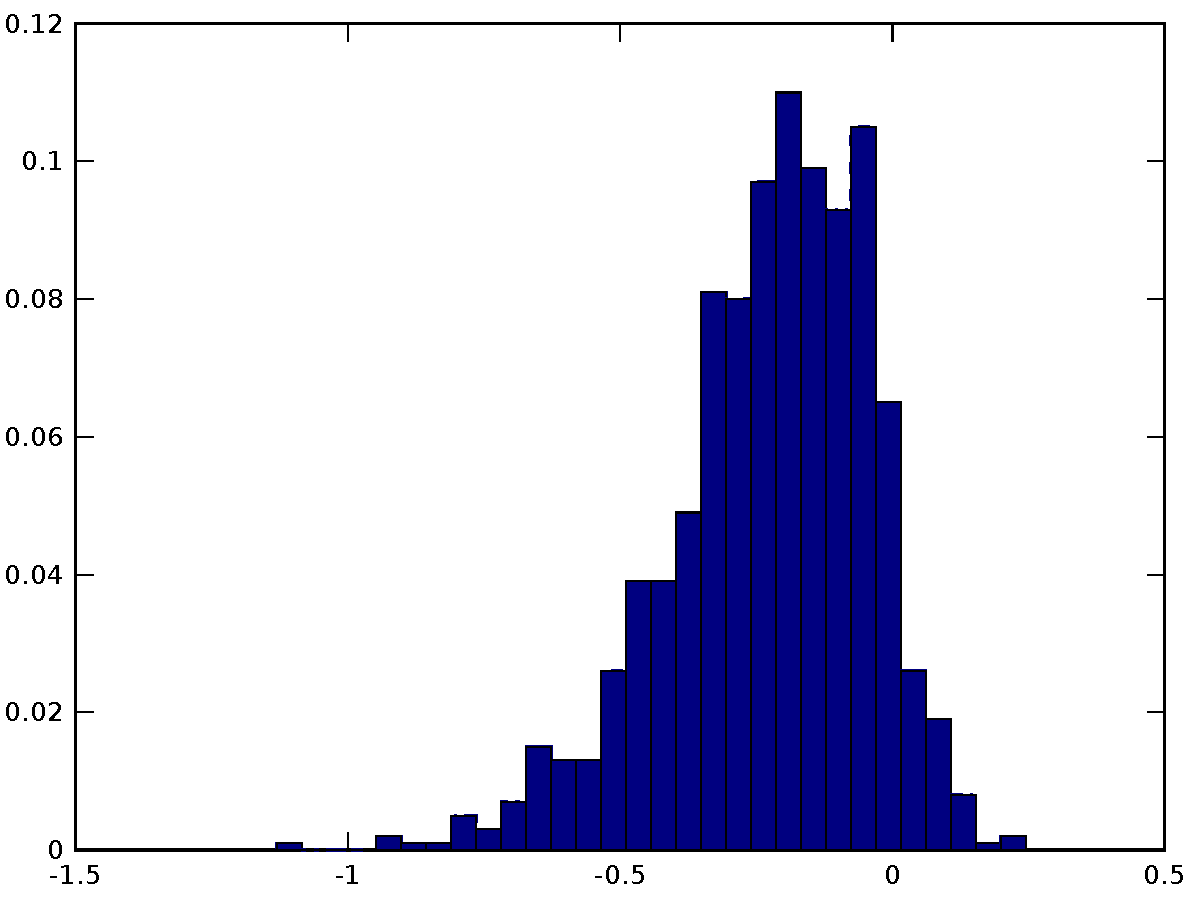
\includegraphics{Examples/OLS/Biased}
\end{figure}
The program that generates the plot is  \htmladdnormallink{Biased.m}{file:///home/michael/Mystuff/Econometrics/Examples/OLS/Biased.m}  , if you would like to experiment with this.


\subsection{Normality}

With the linearity assumption, we have $\hat{\beta}=\beta+(X^{\prime}X)^{-1}X^{\prime}\varepsilon.$ This is a linear function of $\varepsilon$. Adding the assumption of normality (\ref{assumption: normal errors}, which implies strong exogeneity), then

\[
\hat{\beta}\sim N\left(\beta,(X^{\prime}X)^{-1}\sigma_{0}^{2}\right)
\]
since a linear function of a normal random vector is also normally distributed. In Figure \ref{figure-unbiasedness} you can see that the estimator appears to be normally distributed. It in fact is normally distributed, since the DGP (see the Octave program) has normal errors. Even when the data may be taken to be IID, the assumption of normality is often questionable or simply untenable. For example, if the dependent variable is the number of automobile trips per week, it is a count variable with a discrete distribution, and is thus not normally distributed. Many variables in economics can take on only nonnegative values, which, strictly speaking, rules out normality.\footnote{Normality may be a good model nonetheless, as long as the probability of a negative value occuring is negligable under the model. This depends upon the mean being large enough in relation to the variance.}


\subsection{The variance of the OLS estimator and the Gauss-Markov theorem}

Now let's make all the classical assumptions except the assumption of normality. We have $\hat{\beta}=\beta+(X^{\prime}X)^{-1}X^{\prime}\varepsilon$ and we know that $E(\hat{\beta})=\beta$. So
\begin{eqnarray*}
Var(\hat{\beta}) & = & E\left\{ \left(\mathbf{\hat{\beta}-\beta}\right)\left(\mathbf{\hat{\beta}-\beta}\right)^{\prime}\right\} \\
 & = & E\left\{ (X^{\prime}X)^{-1}X^{\prime}\varepsilon\varepsilon^{\prime}X(X^{\prime}X)^{-1}\right\} \\
 & = & (X^{\prime}X)^{-1}\sigma_{0}^{2}
\end{eqnarray*}


The OLS\ estimator is a \emph{linear estimator}\index{estimator, linear}, which means that it is a linear function of the dependent variable, $y.$
\begin{eqnarray*}
\hat{\beta} & = & \left[(X^{\prime}X)^{-1}X^{\prime}\right]y\\
 & = & Cy
\end{eqnarray*}
 where $C$ is a function of the explanatory variables only, not the dependent variable. It is also \emph{unbiased} under the present assumptions, as we proved above. One could consider other weights $W$ that are a function of $X$ that define some other linear estimator. We'll still insist upon unbiasedness. Consider $\tilde{\beta}=Wy,$ where $W=W(X)$ is some $k\times n$ matrix function of $X.$ Note that since $W$ is a function of $X,$ it is nonstochastic, too. If the estimator is unbiased, then we must have $WX=I_{K}$: 
\begin{eqnarray*}
\mathcal{E}(Wy) & = & \mathcal{E}(WX\beta_{0}+W\varepsilon)\\
 & = & WX\beta_{0}\\
 & = & \beta_{0}\\
 & \Rightarrow\\
WX & = & I_{K}
\end{eqnarray*}
 The variance of $\tilde{\beta}$ is 
\[
V(\tilde{\beta})=WW^{\prime}\sigma_{0}^{2}.
\]
 Define 
\[
D=W-(X^{\prime}X)^{-1}X^{\prime}
\]
 so 
\[
W=D+(X^{\prime}X)^{-1}X^{\prime}
\]
 Since $WX=I_{K},$ $DX=0,$ so 
\begin{eqnarray*}
V(\tilde{\beta}) & = & \left(D+(X^{\prime}X)^{-1}X^{\prime}\right)\left(D+(X^{\prime}X)^{-1}X^{\prime}\right)^{\prime}\sigma_{0}^{2}\\
 & = & \left(DD^{\prime}+\left(X^{\prime}X\right)^{-1}\right)\sigma_{0}^{2}
\end{eqnarray*}
 So 
\[
V(\tilde{\beta})\geq V(\hat{\beta})
\]
 The inequality is a shorthand means of expressing, more formally, that $V(\tilde{\beta})-V(\hat{\beta})$ is a positive semi-definite matrix. This is a proof of the Gauss-Markov Theorem. The OLS estimator is the ''best linear unbiased estimator'' (BLUE).
\begin{itemize}
\item It is worth emphasizing again that we have not used the normality assumption in any way to prove the Gauss-Markov theorem, so it is valid if the errors are not normally distributed, as long as the other assumptions hold. 
\end{itemize}
To illustrate the Gauss-Markov result, consider the estimator that results from splitting the sample into $p$ equally-sized parts, estimating using each part of the data separately by OLS, then averaging the $p$ resulting estimators. You should be able to show that this estimator is unbiased, but inefficient with respect to the OLS estimator. The program  \htmladdnormallink{Efficiency.m}{file:///home/michael/Mystuff/Econometrics/Examples/OLS/Efficiency.m}  illustrates this using a small Monte Carlo experiment, which compares the OLS estimator and a 3-way split sample estimator. The data generating process follows the classical model, with $n=21$. The true parameter value is $\beta=2.$ In Figures \ref{cap:Gauss-Markov-Result: OLS} and \ref{cap:Gauss-Markov-Result: split sample} we can see that the OLS estimator is more efficient, since the tails of its histogram are more narrow. 
\begin{figure}
\caption{\label{cap:Gauss-Markov-Result: OLS}Gauss-Markov Result: The OLS estimator}


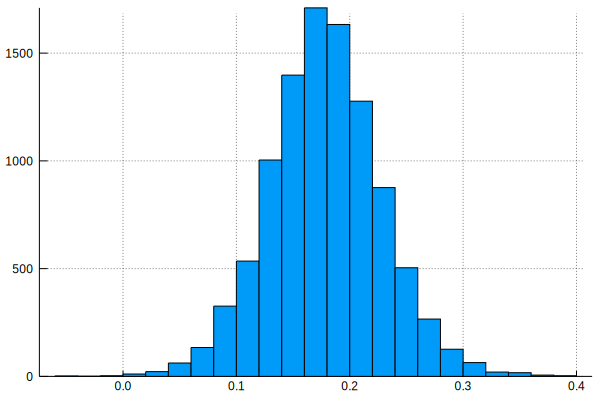
\includegraphics[width=12cm]{Examples/OLS/efficiency-1}
\end{figure}
\begin{figure}
\caption{Gauss-Markov Resul\label{cap:Gauss-Markov-Result: split sample}: The split sample estimator}


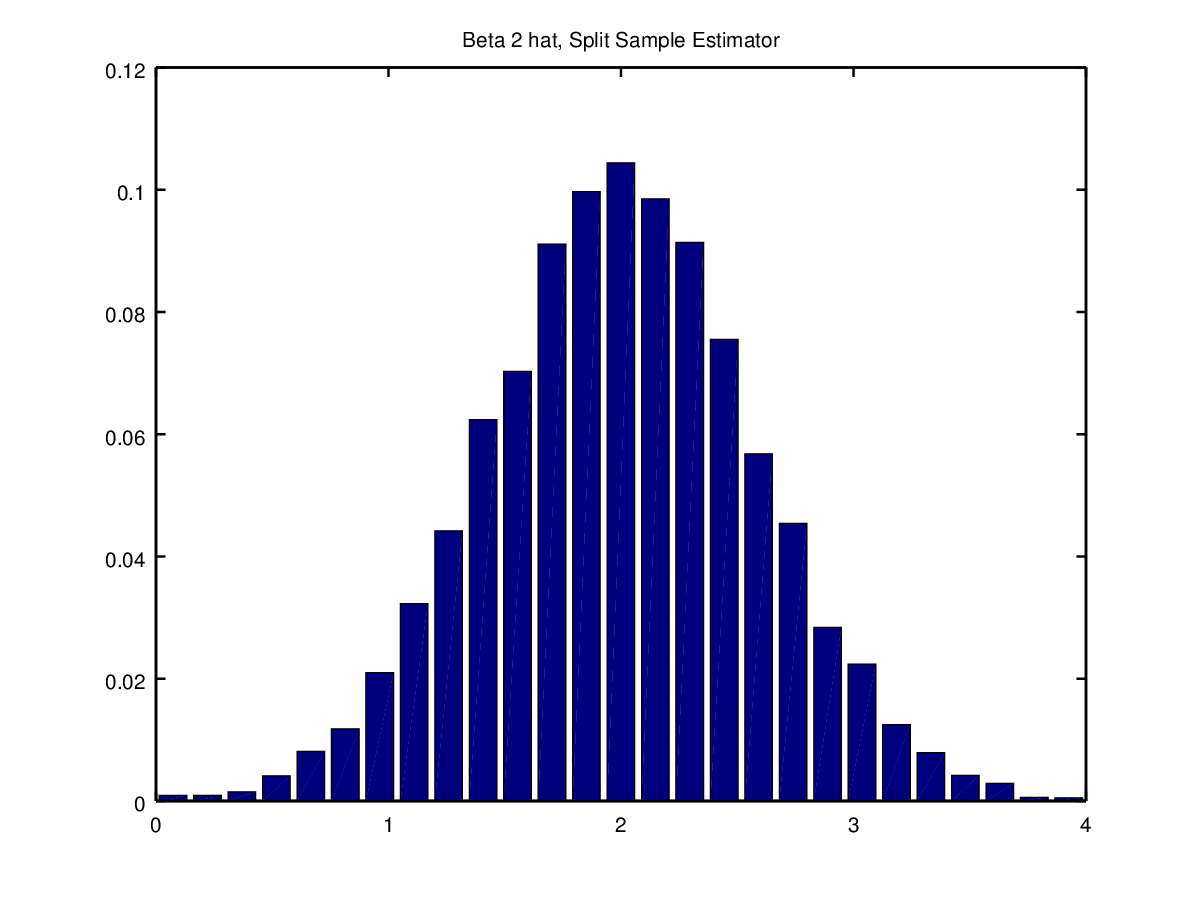
\includegraphics[width=12cm]{Examples/OLS/efficiency-2}
\end{figure}


We have that $E(\hat{\beta})=\beta$ and $Var(\hat{\beta})=\left(X^{'}X\right)^{-1}\sigma_{0}^{2},$ but we still need to estimate the variance of $\epsilon$, $\sigma_{0}^{2}$, in order to have an idea of the precision of the estimates of $\beta$. A commonly used estimator of $\sigma_{0}^{2}$ is 
\[
\widehat{\sigma_{0}^{2}}=\frac{1}{n-K}\hat{\varepsilon}^{\prime}\hat{\varepsilon}
\]
This estimator is unbiased:

\begin{eqnarray*}
\widehat{\sigma_{0}^{2}} & = & \frac{1}{n-K}\hat{\varepsilon}^{\prime}\hat{\varepsilon}\\
 & = & \frac{1}{n-K}\varepsilon^{\prime}M\varepsilon\\
\mathcal{E}(\widehat{\sigma_{0}^{2}}) & = & \frac{1}{n-K}E(Tr\varepsilon^{\prime}M\varepsilon)\\
 & = & \frac{1}{n-K}E(TrM\varepsilon\varepsilon^{\prime})\\
 & = & \frac{1}{n-K}TrE(M\varepsilon\varepsilon^{\prime})\\
 & = & \frac{1}{n-K}\sigma_{0}^{2}TrM\\
 & = & \frac{1}{n-K}\sigma_{0}^{2}\left(n-k\right)\\
 & = & \sigma_{0}^{2}
\end{eqnarray*}
where we use the fact that $Tr(AB)=Tr(BA)$ when both products are conformable. Thus, this estimator is also unbiased under these assumptions.


\section{\label{sec:Example:-The-Nerlove}Example: The Nerlove model }


\subsection{Theoretical background}

For a firm that takes input prices $w$ and the output level $q$ as given, the cost minimization problem is to choose the quantities of inputs $x$ to solve the problem

\[
\min_{x}w'x
\]
 subject to the restriction

\[
f(x)=q.
\]
 The solution is the vector of factor demands $x(w,q)$. The \emph{cost function} is obtained by substituting the factor demands into the criterion function: 
\[
Cw,q)=w'x(w,q).
\]
 
\begin{itemize}
\item \textbf{Monotonicity} Increasing factor prices cannot decrease cost, so 
\[
\frac{\partial C(w,q)}{\partial w}\geq0
\]
Remember that these derivatives give the conditional factor demands (Shephard's Lemma).
\item \textbf{Homogeneity} The cost function is homogeneous of degree 1 in input prices: $C(tw,q)=tC(w,q)$ where $t$ is a scalar constant. This is because the factor demands are homogeneous of degree zero in factor prices - they only depend upon relative prices.
\item \textbf{Returns to scale} The \emph{returns to scale} parameter $\gamma$ is defined as the inverse of the elasticity of cost with respect to output:
\[
\gamma=\left(\frac{\partial C(w,q)}{\partial q}\frac{q}{C(w,q)}\right)^{-1}
\]
\emph{Constant returns to scale} is the case where increasing production $q$ implies that cost increases in the proportion 1:1. If this is the case, then $\gamma=1$.
\end{itemize}

\subsection{Cobb-Douglas functional form}

The Cobb-Douglas functional form is linear in the logarithms of the regressors and the dependent variable. For a cost function, if there are $g$ factors, the Cobb-Douglas cost function has the form

\[
C=Aw_{1}^{\beta_{1}}...w_{g}^{\beta_{g}}q^{\beta_{q}}e^{\varepsilon}
\]
What is the elasticity of $C$ with respect to $w_{j}$?
\begin{eqnarray*}
e_{w_{j}}^{C} & = & \left(\frac{\partial C}{\partial_{W_{J}}}\right)\left(\frac{w_{j}}{C}\right)\\
 & = & \beta_{j}Aw_{1}^{\beta_{1}}.w_{j}^{\beta_{j}-1}..w_{g}^{\beta_{g}}q^{\beta_{q}}e^{\varepsilon}\frac{w_{j}}{Aw_{1}^{\beta_{1}}...w_{g}^{\beta_{g}}q^{\beta_{q}}e^{\varepsilon}}\\
 & = & \beta_{j}
\end{eqnarray*}
This is one of the reasons the Cobb-Douglas form is popular - the coefficients are easy to interpret, since they are the elasticities of the dependent variable with respect to the explanatory variable. Not that in this case,
\begin{eqnarray*}
e_{w_{j}}^{C} & = & \left(\frac{\partial C}{\partial_{W_{J}}}\right)\left(\frac{w_{j}}{C}\right)\\
 & = & x_{j}(w,q)\frac{w_{j}}{C}\\
 & \equiv & s_{j}(w,q)
\end{eqnarray*}
the \emph{cost share} of the $j^{th}$ input. So with a Cobb-Douglas cost function, $\beta_{j}=s_{j}(w,q)$. The cost shares are constants.

Note that after a logarithmic transformation we obtain
\[
\ln C=\alpha+\beta_{1}\ln w_{1}+...+\beta_{g}\ln w_{g}+\beta_{q}\ln q+\epsilon
\]
where $\alpha=\ln A$ . So we see that the transformed model is linear in the logs of the data.

One can verify that the property of HOD1 implies that 
\[
\sum_{i=1}^{g}\beta_{g}=1
\]
In other words, the cost shares add up to 1. 

The hypothesis that the technology exhibits CRTS implies that 
\[
\gamma=\frac{1}{\beta_{q}}=1
\]
so $\beta_{q}=1.$ Likewise, monotonicity implies that the coefficients $\beta_{i}\geq0,i=1,...,g$.


\subsection{The Nerlove data and OLS\label{sub:The-Nerlove-data}}

The file \htmladdnormallink{nerlove.data}{file:///home/michael/Mystuff/Econometrics/Examples/Data/nerlove.data}  contains data on 145 electric utility companies' cost of production, output and input prices. The data are for the U.S., and were collected by M. Nerlove. The observations are by row, and the columns are \textbf{COMPANY, COST} $(C)$\textbf{, OUTPUT} $(Q),$ \textbf{PRICE\ OF LABOR} $(P_{L})$, \textbf{PRICE OF\ FUEL} $(P_{F})$ and \textbf{PRICE OF\ CAPITAL} $(P_{K}).$ Note that the data are sorted by output level (the third column).

We will estimate the Cobb-Douglas model 
\begin{equation}
\ln C=\beta_{1}+\beta_{Q}\ln Q+\beta_{L}\ln P_{L}+\beta_{F}\ln P_{F}+\beta_{K}\ln P_{K}+\epsilon\label{simple nerlove model}
\end{equation}
 using OLS. To do this yourself, you need the data file mentioned above, as well as  \htmladdnormallink{Nerlove.m}{file:///home/michael/Mystuff/Econometrics/Examples/OLS/Nerlove.m}  (the estimation program), and the library of Octave functions mentioned in the introduction to Octave that forms section \ref{sec:Introduction-to-Octave} of this document.\footnote{If you are running the bootable CD, you have all of this installed and ready to run.} 

\begin{singlespace}
The results are 

\verbatiminput{Examples/OLS/nerlove.out}
\end{singlespace}
\begin{itemize}
\item Do the theoretical restrictions hold?
\item Does the model fit well?
\item What do you think about RTS?
\end{itemize}
While we will most often use Octave programs as examples in this document, since following the programming statements is a useful way of learning how theory is put into practice, you may be interested in a more ''user-friendly'' environment for doing econometrics. I heartily recommend \htmladdnormallink{Gretl}{http://gretl.sourceforge.net}, the Gnu Regression, Econometrics, and Time-Series Library. This is an easy to use program, available in English, French, and Spanish, and it comes with a lot of data ready to use. It even has an option to save output as \LaTeX{} fragments, so that I can just include the results into this document, no muss, no fuss. Here is the Nerlove data in the form of a GRETL data set:  \htmladdnormallink{nerlove.gdt}{file:///home/michael/Mystuff/Econometrics/Examples/Data/nerlove.gdt} . Here the results of the Nerlove model from GRETL: \begin{center}

Model 2: OLS estimates using the 145 observations 1--145\\
Dependent variable: l\_cost\\

\vspace{1em}

\begin{tabular*}{\textwidth}{@{\extracolsep{\fill}}
l% col 1: varname
  D{.}{.}{-1}% col 2: coeff
    D{.}{.}{-1}% col 3: sderr
      D{.}{.}{-1}% col 4: t-stat
        D{.}{.}{4}}% col 5: p-value (or slope)
Variable &
  \multicolumn{1}{c}{Coefficient} &
    \multicolumn{1}{c}{Std.\ Error} &
      \multicolumn{1}{c}{$t$-statistic} &
        \multicolumn{1}{c}{p-value} \\[1ex]
const &
  -3.5265 &
    1.77437 &
      -1.9875 &
        0.0488 \\
l\_output &
  0.720394 &
    0.0174664 &
      41.2445 &
        0.0000 \\
l\_labor &
  0.436341 &
    0.291048 &
      1.4992 &
        0.1361 \\
l\_fuel &
  0.426517 &
    0.100369 &
      4.2495 &
        0.0000 \\
l\_capita &
  -0.219888 &
    0.339429 &
      -0.6478 &
        0.5182 \\
\end{tabular*}

\vspace{1em}

\begin{tabular}{lD{.}{.}{-1}}
Mean of dependent variable & 1.72466 \\
 S.D. of dependent variable & 1.42172 \\
Sum of squared residuals & 21.5520 \\
Standard error of residuals ($\hat{\sigma}$) & 0.392356 \\
Unadjusted $R^2$ & 0.925955 \\
Adjusted $\bar{R}^2$ & 0.923840 \\
$F(4, 140)$ & 437.686 \\
Akaike information criterion & 145.084 \\
Schwarz Bayesian criterion & 159.967 \\
\end{tabular}


\end{center}
 Fortunately, Gretl and my OLS program agree upon the results. Gretl is included in the bootable CD mentioned in the introduction. I recommend using GRETL to repeat the examples that are done using Octave. 

The previous properties hold for finite sample sizes. Before considering the asymptotic properties of the OLS\ estimator it is useful to review the MLE estimator, since under the assumption of normal errors the two estimators coincide.


\section{Exercises}
\begin{enumerate}
\item Prove that the split sample estimator used to generate figure \ref{cap:Gauss-Markov-Result: split sample} is unbiased.
\item Calculate the OLS estimates of the Nerlove model using Octave and GRETL, and provide printouts of the results. Interpret the results. 
\item Do an analysis of whether or not there are influential observations for OLS estimation of the Nerlove model. Discuss.
\item Using GRETL, examine the residuals after OLS estimation and tell me whether or not you believe that the assumption of independent identically distributed normal errors is warranted. No need to do formal tests, just look at the plots. Print out any that you think are relevant, and interpret them.
\item For a random vector $X\sim N(\mu_{x},\Sigma),$ what is the distribution of $AX+b$, where $A$ and $b$ are conformable matrices of constants?
\item Using Octave, write a little program that verifies that $Tr(AB)=Tr(BA)$ for $A$ and $B$ 4x4 matrices of random numbers. Note: there is an Octave function \texttt{trace.}
\item For the model with a constant and a single regressor, $y_{t}=\beta_{1}+\beta_{2}x_{t}+\epsilon_{t}$, which satisfies the classical assumptions, prove that the variance of the OLS estimator declines to zero as the sample size increases.
\end{enumerate}
\newpage

\newpage{}


\chapter{Asymptotic properties of the least squares estimator}

The OLS estimator under the classical assumptions is BLUE\footnote{BLUE $\equiv$ best linear unbiased estimator if I haven't defined it before}, for all sample sizes. Now let's see what happens when the sample size tends to infinity. 


\section{Consistency}

\begin{eqnarray*}
\hat{\beta} & = & (X^{\prime}X)^{-1}X^{\prime}y\\
 & = & (X^{\prime}X)^{-1}X^{\prime}\left(X\beta+\varepsilon\right)\\
 & = & \beta_{0}+(X^{\prime}X)^{-1}X^{\prime}\varepsilon\\
 & = & \beta_{0}+\left(\frac{X^{\prime}X}{n}\right)^{-1}\frac{X^{\prime}\varepsilon}{n}
\end{eqnarray*}
 Consider the last two terms. By assumption $\lim_{n\rightarrow\infty}\left(\frac{X^{\prime}X}{n}\right)=Q_{X}\Rightarrow\lim_{n\rightarrow\infty}\left(\frac{X^{\prime}X}{n}\right)^{-1}=Q_{X}^{-1},$ since the inverse of a nonsingular matrix is a continuous function of the elements of the matrix. Considering $\frac{X^{\prime}\varepsilon}{n},$
\[
\frac{X^{\prime}\varepsilon}{n}=\frac{1}{n}\sum_{t=1}^{n}x_{t}\varepsilon_{t}
\]
 Each $x_{t}\varepsilon_{t}$ has expectation zero, so 
\[
E\left(\frac{X^{\prime}\varepsilon}{n}\right)=0
\]
The variance of each term is
\begin{eqnarray*}
V\left(x_{t}\epsilon_{t}\right) & = & x_{t}x_{t}^{\prime}\sigma^{2}.
\end{eqnarray*}
As long as these are finite, and given a technical condition\footnote{For application of LLN's and CLT's, of which there are very many to choose from, I'm going to avoid the technicalities. Basically, as long as terms that make up an average have finite variances and are not too strongly dependent, one will be able to find a LLN or CLT to apply. Which one it is doesn't matter, we only need the result.}, the Kolmogorov SLLN applies, so
\[
\frac{1}{n}\sum_{t=1}^{n}x_{t}\varepsilon_{t}\overset{a.s.}{\rightarrow}0.
\]
 This implies that 
\[
\hat{\beta}\overset{a.s.}{\rightarrow}\beta_{0}.
\]
 This is the property of \emph{strong consistency:} the estimator converges in almost surely to the true value.
\begin{itemize}
\item The consistency proof does not use the normality assumption. 
\item Remember that almost sure convergence implies convergence in probability.
\end{itemize}

\section{Asymptotic normality}

We've seen that the OLS estimator is normally distributed \emph{under the assumption of normal errors.} If the error distribution is unknown, we of course don't know the distribution of the estimator. However, we can get asymptotic results. \emph{Assuming the distribution of} $\varepsilon$ is unknown, but the the other classical assumptions hold:

\begin{eqnarray*}
\hat{\beta} & = & \beta_{0}+(X^{\prime}X)^{-1}X^{\prime}\varepsilon\\
\hat{\beta}-\beta_{0} & = & (X^{\prime}X)^{-1}X^{\prime}\varepsilon\\
\sqrt{n}\left(\hat{\beta}-\beta_{0}\right) & = & \left(\frac{X^{\prime}X}{n}\right)^{-1}\frac{X^{\prime}\varepsilon}{\sqrt{n}}
\end{eqnarray*}

\begin{itemize}
\item Now as before, $\left(\frac{X^{\prime}X}{n}\right)^{-1}\rightarrow Q_{X}^{-1}.$
\item Considering $\frac{X^{\prime}\varepsilon}{\sqrt{n}},$ the limit of the variance is 
\begin{eqnarray*}
\lim_{n\rightarrow\infty}V\left(\frac{X^{\prime}\varepsilon}{\sqrt{n}}\right) & = & \lim_{n\rightarrow\infty}E\left(\frac{X^{\prime}\epsilon\epsilon^{\prime}X}{n}\right)\\
 & = & \sigma_{0}^{2}Q_{X}
\end{eqnarray*}
 The mean is of course zero. To get asymptotic normality, we need to apply a CLT. We assume one (for instance, the Lindeberg-Feller CLT) holds, so
\[
\frac{X^{\prime}\varepsilon}{\sqrt{n}}\overset{d}{\rightarrow}N\left(0,\sigma_{0}^{2}Q_{X}\right)
\]
 Therefore, 
\begin{equation}
\sqrt{n}\left(\hat{\beta}-\beta_{0}\right)\overset{d}{\rightarrow}N\left(0,\sigma_{0}^{2}Q_{X}^{-1}\right)\label{eq:asymp normality OLS}
\end{equation}

\item In summary, the OLS estimator is normally distributed in small and large samples if $\varepsilon$ is normally distributed. If $\varepsilon$ is not normally distributed, $\hat{\beta}$ is asymptotically normally distributed when a CLT can be applied.
\end{itemize}

\section{Asymptotic efficiency\label{sec:Asymptotic-efficiency}}

The least squares objective function is 

\begin{eqnarray*}
s(\beta) & = & \sum_{t=1}^{n}\left(y_{t}-x_{t}^{\prime}\beta\right)^{2}
\end{eqnarray*}
 Supposing that $\varepsilon$ is normally distributed, the model is 
\[
y=X\beta_{0}+\varepsilon,
\]
\begin{eqnarray*}
\varepsilon & \sim & N(0,\sigma_{0}^{2}I_{n}),\textrm{ so}\\
f(\varepsilon) & = & \prod_{t=1}^{n}\frac{1}{\sqrt{2\pi\sigma^{2}}}\exp\left(-\frac{\varepsilon_{t}^{2}}{2\sigma^{2}}\right)
\end{eqnarray*}
 The joint density for $y$ can be constructed using a change of variables. We have $\varepsilon=y-X\beta,$ so $\frac{\partial\varepsilon}{\partial y^{\prime}}=I_{n}$ and $|\frac{\partial\varepsilon}{\partial y^{\prime}}|=1,$ so 
\[
f(y)=\prod_{t=1}^{n}\frac{1}{\sqrt{2\pi\sigma^{2}}}\exp\left(-\frac{(y_{t}-x_{t}^{\prime}\beta)^{2}}{2\sigma^{2}}\right).
\]
 Taking logs, 
\[
\ln L(\beta,\sigma)=-n\ln\sqrt{2\pi}-n\ln\sigma-\sum_{t=1}^{n}\frac{\left(y_{t}-x_{t}'\beta\right)^{2}}{2\sigma^{2}}.
\]
 Maximizing this function with respect to $\beta$ and $\sigma$ gives what is known as the maximum likelihood (ML) estimator. It turns out that ML estimators are asymptotically efficient, a concept that will be explained in detail later. It's clear that the first order conditions for the MLE of $\beta_{0}$ are the same as the first order conditions that define the OLS estimator (up to multiplication by a constant), so the OLS estimator of $\beta$ is also the ML estimator. \emph{The estimators are the same, under the present assumptions.} Therefore, their properties are the same. \emph{In particular, under the classical assumptions with normality, the OLS\ estimator} $\hat{\beta}$ \emph{is asymptotically efficient. }Note that one needs to make an assumption about the distribution of the errors to compute the ML estimator. If the errors had a distribution other than the normal, then the OLS estimator and the ML estimator would not coincide.

As we'll see later, it will be possible to use (iterated) linear estimation methods and still achieve asymptotic efficiency even if the assumption that $Var(\varepsilon)\neq\sigma^{2}I_{n},$ as long as $\varepsilon$ is still normally distributed. This is \textbf{not} the case if $\varepsilon$ is nonnormal. In general with nonnormal errors it will be necessary to use nonlinear estimation methods to achieve asymptotically efficient estimation. 


\section{Exercises}
\begin{enumerate}
\item Write an Octave program that generates a histogram for $R$ Monte Carlo replications of $\sqrt{n}\left(\hat{\beta}_{j}-\beta_{j}\right)$, where $\hat{\beta}$ is the OLS estimator and $\beta_{j}$ is one of the $k$ slope parameters. $R$ should be a large number, at least 1000. The model used to generate data should follow the classical assumptions, except that the errors should not be normally distributed (try $U(-a,a)$, $t(p)$, $\chi^{2}(p)-p,$ etc). Generate histograms for $n\in\left\{ 20,50,100,1000\right\} $. Do you observe evidence of asymptotic normality? Comment.
\end{enumerate}
\newpage


\chapter{Restrictions and hypothesis tests}


\section{Exact linear restrictions}

In many cases, economic theory suggests restrictions on the parameters of a model. For example, a demand function is supposed to be homogeneous of degree zero in prices and income. If we have a Cobb-Douglas (log-linear) model, 
\[
\ln q=\beta_{0}+\beta_{1}\ln p_{1}+\beta_{2}\ln p_{2}+\beta_{3}\ln m+\varepsilon,
\]
 then we need that 
\[
k^{0}\ln q=\beta_{0}+\beta_{1}\ln kp_{1}+\beta_{2}\ln kp_{2}+\beta_{3}\ln km+\varepsilon,
\]
 so 
\begin{eqnarray*}
\beta_{1}\ln p_{1}+\beta_{2}\ln p_{2}+\beta_{3}\ln m & = & \beta_{1}\ln kp_{1}+\beta_{2}\ln kp_{2}+\beta_{3}\ln km\\
 & = & \left(\ln k\right)(\beta_{1}+\beta_{2}+\beta_{3})+\beta_{1}\ln p_{1}+\beta_{2}\ln p_{2}+\beta_{3}\ln m.
\end{eqnarray*}
 The only way to guarantee this for arbitrary $k$ is to set 
\[
\beta_{1}+\beta_{2}+\beta_{3}=0,
\]
 which is a \emph{parameter restriction.} In particular, this is a linear equality restriction, which is probably the most commonly encountered case.


\subsection{Imposition}

The general formulation of linear equality restrictions is the model 
\begin{eqnarray*}
y & = & X\beta+\varepsilon\\
R\beta & = & r
\end{eqnarray*}
 where $R$ is a $Q\times K$ matrix, $Q<K$ and $r$ is a $Q\times1$ vector of constants.
\begin{itemize}
\item We assume $R$ is of rank $Q,$ so that there are no redundant restrictions.
\item We also assume that $\exists\beta$ that satisfies the restrictions: they aren't infeasible. 
\end{itemize}
Let's consider how to estimate $\beta$ subject to the restrictions $R\beta=r.$ The most obvious approach is to set up the Lagrangean 
\[
\min_{\beta,\lambda}s(\beta,\lambda)=\frac{1}{n}\left(y-X\beta\right)^{\prime}\left(y-X\beta\right)+2\lambda^{\prime}(R\beta-r).
\]
 The Lagrange multipliers are scaled by 2, which makes things less messy. The fonc are 
\begin{eqnarray*}
D_{\beta}s(\hat{\beta},\hat{\lambda}) & = & -2X^{\prime}y+2X^{\prime}X\hat{\beta}_{R}+2R^{\prime}\hat{\lambda}\equiv0\\
D_{\lambda}s(\hat{\beta},\hat{\lambda}) & = & R\hat{\beta}_{R}-r\equiv0,
\end{eqnarray*}
 which can be written as 
\[
\left[\begin{array}{cc}
X^{\prime}X & R^{\prime}\\
R & 0
\end{array}\right]\left[\begin{array}{c}
\hat{\beta}_{R}\\
\hat{\lambda}
\end{array}\right]=\left[\begin{array}{c}
X^{\prime}y\\
r
\end{array}\right].
\]
 We get 
\[
\left[\begin{array}{c}
\hat{\beta}_{R}\\
\hat{\lambda}
\end{array}\right]=\left[\begin{array}{cc}
X^{\prime}X & R^{\prime}\\
R & 0
\end{array}\right]^{-1}\left[\begin{array}{c}
X^{\prime}y\\
r
\end{array}\right].
\]
 Maybe you're curious about how to invert a partitioned matrix? I can help you with that:

Note that 
\begin{eqnarray*}
\left[\begin{array}{cc}
\left(X^{\prime}X\right)^{-1} & 0\\
-R\left(X^{\prime}X\right)^{-1} & I_{Q}
\end{array}\right]\left[\begin{array}{cc}
X^{\prime}X & R^{\prime}\\
R & 0
\end{array}\right] & \equiv & AB\\
 & = & \left[\begin{array}{cc}
I_{K} & \left(X^{\prime}X\right)^{-1}R^{\prime}\\
0 & -R\left(X^{\prime}X\right)^{-1}R^{\prime}
\end{array}\right]\\
 & \equiv & \left[\begin{array}{cc}
I_{K} & \left(X^{\prime}X\right)^{-1}R^{\prime}\\
0 & -P
\end{array}\right]\\
 & \equiv & C,
\end{eqnarray*}
 and 
\begin{eqnarray*}
\left[\begin{array}{cc}
I_{K} & (X^{\prime}X)^{-1}R^{\prime}P^{-1}\\
0 & -P^{-1}
\end{array}\right]\left[\begin{array}{cc}
I_{K} & \left(X^{\prime}X\right)^{-1}R^{\prime}\\
0 & -P
\end{array}\right] & \equiv & DC\\
 & = & I_{K+Q},
\end{eqnarray*}
 so 
\begin{eqnarray*}
DAB & = & I_{K+Q}\\
DA & = & B^{-1}\\
B^{-1} & = & \left[\begin{array}{cc}
I_{K} & (X^{\prime}X)^{-1}R^{\prime}P^{-1}\\
0 & -P^{-1}
\end{array}\right]\left[\begin{array}{cc}
\left(X^{\prime}X\right)^{-1} & 0\\
-R\left(X^{\prime}X\right)^{-1} & I_{Q}
\end{array}\right]\\
 & = & \left[\begin{array}{cc}
\left(X^{\prime}X\right)^{-1}-(X^{\prime}X)^{-1}R^{\prime}P^{-1}R\left(X^{\prime}X\right)^{-1} & (X^{\prime}X)^{-1}R^{\prime}P^{-1}\\
P^{-1}R\left(X^{\prime}X\right)^{-1} & -P^{-1}
\end{array}\right],
\end{eqnarray*}
If you weren't curious about that, please start paying attention again. Also, note that we have made the definition $P=R\left(X^{\prime}X\right)^{-1}R^{\prime}$)
\begin{eqnarray*}
\left[\begin{array}{c}
\hat{\beta}_{R}\\
\hat{\lambda}
\end{array}\right] & = & \left[\begin{array}{cc}
\left(X^{\prime}X\right)^{-1}-(X^{\prime}X)^{-1}R^{\prime}P^{-1}R\left(X^{\prime}X\right)^{-1} & (X^{\prime}X)^{-1}R^{\prime}P^{-1}\\
P^{-1}R\left(X^{\prime}X\right)^{-1} & -P^{-1}
\end{array}\right]\left[\begin{array}{c}
X^{\prime}y\\
r
\end{array}\right]\\
 & = & \left[\begin{array}{c}
\hat{\beta}-(X^{\prime}X)^{-1}R^{\prime}P^{-1}\left(R\hat{\beta}-r\right)\\
P^{-1}\left(R\hat{\beta}-r\right)
\end{array}\right]\\
 & = & \left[\begin{array}{c}
\left(I_{K}-(X^{\prime}X)^{-1}R^{\prime}P^{-1}R\right)\\
P^{-1}R
\end{array}\right]\hat{\beta}+\left[\begin{array}{c}
(X^{\prime}X)^{-1}R^{\prime}P^{-1}r\\
-P^{-1}r
\end{array}\right]
\end{eqnarray*}
 The fact that $\hat{\beta}_{R}$ and $\hat{\lambda}$ are linear functions of $\hat{\beta}$ makes it easy to determine their distributions, since the distribution of $\hat{\beta}$ is already known. Recall that for $x$ a random vector, and for $A$ and $b$ a matrix and vector of constants, respectively, $Var\left(Ax+b\right)=AVar(x)A^{\prime}.$

Though this is the obvious way to go about finding the restricted estimator, an easier way, if the number of restrictions is small, is to impose them by substitution. Write 
\begin{eqnarray*}
y & = & X_{1}\beta_{1}+X_{2}\beta_{2}+\varepsilon\\
\left[\begin{array}{cc}
R_{1} & R_{2}\end{array}\right]\left[\begin{array}{c}
\beta_{1}\\
\beta_{2}
\end{array}\right] & = & r
\end{eqnarray*}
 where $R_{1}$ is $Q\times Q$ nonsingular. Supposing the $Q$ restrictions are linearly independent, one can always make $R_{1}$ nonsingular by reorganizing the columns of $X.$ Then 
\[
\beta_{1}=R_{1}^{-1}r-R_{1}^{-1}R_{2}\beta_{2}.
\]
 Substitute this into the model 
\begin{eqnarray*}
y & = & X_{1}R_{1}^{-1}r-X_{1}R_{1}^{-1}R_{2}\beta_{2}+X_{2}\beta_{2}+\varepsilon\\
y-X_{1}R_{1}^{-1}r & = & \left[X_{2}-X_{1}R_{1}^{-1}R_{2}\right]\beta_{2}+\varepsilon
\end{eqnarray*}
 or with the appropriate definitions, 
\[
y_{R}=X_{R}\beta_{2}+\varepsilon.
\]
 This model satisfies the classical assumptions, \emph{supposing the restriction is true}. One can estimate by OLS. The variance of $\hat{\beta}_{2}$ is as before 
\[
V(\hat{\beta}_{2})=\left(X_{R}^{\prime}X_{R}\right)^{-1}\sigma_{0}^{2}
\]
 and the estimator is 
\[
\hat{V}(\hat{\beta}_{2})=\left(X_{R}^{\prime}X_{R}\right)^{-1}\hat{\sigma}^{2}
\]
 where one estimates $\sigma_{0}^{2}$ in the normal way, using the restricted model, \emph{i.e.,}
\[
\widehat{\sigma_{0}^{2}}=\frac{\left(y_{R}-X_{R}\widehat{\beta_{2}}\right)^{\prime}\left(y_{R}-X_{R}\widehat{\beta_{2}}\right)}{n-\left(K-Q\right)}
\]
 To recover $\hat{\beta}_{1},$ use the restriction. To find the variance of $\hat{\beta}_{1},$ use the fact that it is a linear function of $\hat{\beta}_{2},$ so 
\begin{eqnarray*}
V(\hat{\beta}_{1}) & = & R_{1}^{-1}R_{2}V(\hat{\beta}_{2})R_{2}^{\prime}\left(R_{1}^{-1}\right)^{\prime}\\
 & = & R_{1}^{-1}R_{2}\left(X_{2}^{\prime}X_{2}\right)^{-1}R_{2}^{\prime}\left(R_{1}^{-1}\right)^{\prime}\sigma_{0}^{2}
\end{eqnarray*}



\subsection{Properties of the restricted estimator}

We have that 
\begin{eqnarray*}
\hat{\beta}_{R} & = & \hat{\beta}-(X^{\prime}X)^{-1}R^{\prime}P^{-1}\left(R\hat{\beta}-r\right)\\
 & = & \hat{\beta}+(X^{\prime}X)^{-1}R^{\prime}P^{-1}r-(X^{\prime}X)^{-1}R^{\prime}P^{-1}R(X^{\prime}X)^{-1}X^{\prime}y\\
 & = & \beta+(X^{\prime}X)^{-1}X^{\prime}\varepsilon+(X^{\prime}X)^{-1}R^{\prime}P^{-1}\left[r-R\beta\right]-(X^{\prime}X)^{-1}R^{\prime}P^{-1}R(X^{\prime}X)^{-1}X^{\prime}\varepsilon\\
\hat{\beta}_{R}-\beta & = & (X^{\prime}X)^{-1}X^{\prime}\varepsilon\\
 & + & (X^{\prime}X)^{-1}R^{\prime}P^{-1}\left[r-R\beta\right]\\
 & - & (X^{\prime}X)^{-1}R^{\prime}P^{-1}R(X^{\prime}X)^{-1}X^{\prime}\varepsilon
\end{eqnarray*}
 Mean squared error is 
\[
MSE(\hat{\beta}_{R})=\mathcal{E}(\hat{\beta}_{R}-\beta)(\hat{\beta}_{R}-\beta)^{\prime}
\]
 Noting that the crosses between the second term and the other terms expect to zero, and that the cross of the first and third has a cancellation with the square of the third, we obtain 
\begin{eqnarray*}
MSE(\hat{\beta}_{R}) & = & (X^{\prime}X)^{-1}\sigma^{2}\\
 & + & (X^{\prime}X)^{-1}R^{\prime}P^{-1}\left[r-R\beta\right]\left[r-R\beta\right]^{\prime}P^{-1}R(X^{\prime}X)^{-1}\\
 & - & (X^{\prime}X)^{-1}R^{\prime}P^{-1}R(X^{\prime}X)^{-1}\sigma^{2}
\end{eqnarray*}
 So, the first term is the OLS covariance. The second term is PSD, and the third term is NSD.
\begin{itemize}
\item If the restriction is true, the second term is 0, so we are better off. \emph{True restrictions improve efficiency of estimation.}
\item If the restriction is false, we may be better or worse off, in terms of MSE, depending on the magnitudes of $r-R\beta$ and $\sigma^{2}.$
\end{itemize}

\section{Testing}

In many cases, one wishes to test economic theories. If theory suggests parameter restrictions, as in the above homogeneity example, one can test theory by testing parameter restrictions. A number of tests are available. The first two (t and F) have a known small sample distributions, when the errors are normally distributed. The third and fourth (Wald and score) do not require normality of the errors, but their distributions are known only approximately, so that they are not exactly valid with finite samples.


\subsection{t-test}

Suppose one has the model

\[
y=X\beta+\varepsilon
\]
 and one wishes to test the \emph{single restriction} $H_{0}:$$R\beta=r$ vs. $H_{A}:$$R\beta\neq r$ . Under $H_{0},$ with normality of the errors, 
\[
R\hat{\beta}-r\sim N\left(0,R(X^{\prime}X)^{-1}R^{\prime}\sigma_{0}^{2}\right)
\]
 so 
\[
\frac{R\hat{\beta}-r}{\sqrt{R(X^{\prime}X)^{-1}R^{\prime}\sigma_{0}^{2}}}=\frac{R\hat{\beta}-r}{\sigma_{0}\sqrt{R(X^{\prime}X)^{-1}R^{\prime}}}\sim N\left(0,1\right).
\]
 The problem is that $\sigma_{0}^{2}$ is unknown. One could use the consistent estimator $\widehat{\sigma_{0}^{2}}$ in place of $\sigma_{0}^{2},$ but the test would only be valid asymptotically in this case.
\begin{prop}
$\frac{N(0,1)}{\sqrt{\frac{\chi^{2}(q)}{q}}}\sim t(q)$

as long as the $N(0,1)$ and the $\chi^{2}(q)$ are independent. 
\end{prop}
We need a few results on the $\chi{}^{2}$ distribution.
\begin{prop}
If $x\sim N(\mu,I_{n})$ is a vector of $n$ independent r.v.'s., then $x^{\prime}x\sim\chi^{2}(n,\lambda)$ where $\lambda=\sum_{i}\mu_{i}^{2}=\mu^{\prime}\mu$ is the \emph{noncentrality parameter}.
\end{prop}
When a $\chi^{2}$ r.v. has the noncentrality parameter equal to zero, it is referred to as a central $\chi^{2}$ r.v., and it's distribution is written as $\chi^{2}(n),$ suppressing the noncentrality parameter.
\begin{prop}
\label{quadratic form in inverse variance}If the $n$ dimensional random vector $x\sim N(0,V),$ then $x^{\prime}V^{-1}x\sim\chi^{2}(n).$
\end{prop}
We'll prove this one as an indication of how the following unproven propositions could be proved.

Proof: Factor $V^{-1}$ as $P'P$ (this is the Cholesky factorization, where $P$ is defined to be upper triangular). Then consider $y=Px.$ We have 
\[
y\sim N(0,PVP')
\]
 but 
\begin{eqnarray*}
VP'P & = & I_{n}\\
PVP'P & = & P
\end{eqnarray*}
 so $PVP^{\prime}=I_{n}$ and thus $y\sim N(0,I_{n})$. Thus $y^{\prime}y\sim\chi^{2}(n)$ but
\[
y^{\prime}y=x^{\prime}P'Px=xV^{-1}x
\]
 and we get the result we wanted.

A more general proposition which implies this result is
\begin{prop}
If the $n$ dimensional random vector $x\sim N(0,V),$ then $x^{\prime}Bx\sim\chi^{2}(\rho(B))$ if and only if $BV$ is idempotent.
\end{prop}
An immediate consequence is
\begin{prop}
\label{quadratic form in idempotent matrix}If the random vector (of dimension $n$) $x\sim N(0,I),$ and $B$ is idempotent with rank $r,$ then $x^{\prime}Bx\sim\chi^{2}(r)$. 
\end{prop}
Consider the random variable 
\begin{eqnarray*}
\frac{\hat{\varepsilon}^{\prime}\hat{\varepsilon}}{\sigma_{0}^{2}} & = & \frac{\varepsilon^{\prime}M_{X}\varepsilon}{\sigma_{0}^{2}}\\
 & = & \left(\frac{\varepsilon}{\sigma_{0}}\right)^{\prime}M_{X}\left(\frac{\varepsilon}{\sigma_{0}}\right)\\
 & \sim & \chi^{2}(n-K)
\end{eqnarray*}

\begin{prop}
If the random vector (of dimension $n$) $x\sim N(0,I),$ then $Ax$ and $x^{\prime}Bx$ are independent if $AB=0.$
\end{prop}
Now consider (remember that we have only one restriction in this case)

\[
\frac{\frac{R\hat{\beta}-r}{\sigma_{0}\sqrt{R(X^{\prime}X)^{-1}R^{\prime}}}}{\sqrt{\frac{\hat{\varepsilon}^{\prime}\hat{\varepsilon}}{(n-K)\sigma_{0}^{2}}}}=\frac{R\hat{\beta}-r}{\widehat{\sigma_{0}}\sqrt{R(X^{\prime}X)^{-1}R^{\prime}}}
\]
 This will have the $t(n-K)$ distribution if $\hat{\beta}$ and $\hat{\varepsilon}^{\prime}\hat{\varepsilon}$ are independent. But $\hat{\beta}=\beta+(X^{\prime}X)^{-1}X^{\prime}\varepsilon$ and 
\[
(X^{\prime}X)^{-1}X^{\prime}M_{X}=0,
\]
 so 
\[
\frac{R\hat{\beta}-r}{\widehat{\sigma_{0}}\sqrt{R(X^{\prime}X)^{-1}R^{\prime}}}=\frac{R\hat{\beta}-r}{\hat{\sigma}_{R\hat{\beta}}}\sim t(n-K)
\]
 In particular, for the commonly encountered \emph{test of significance} of an individual coefficient, for which $H_{0}:\beta_{i}=0$ vs. $H_{0}:\beta_{i}\neq0$ , the test statistic is 
\[
\frac{\hat{\beta}_{i}}{\hat{\sigma}_{\hat{\beta}i}}\sim t(n-K)
\]

\begin{itemize}
\item \textbf{Note}: the $t-$ test is strictly valid only if the errors are actually normally distributed. If one has nonnormal errors, one could use the above asymptotic result to justify taking critical values from the $N(0,1)$ distribution, since $t(n-K)\overset{d}{\rightarrow}N(0,1)$ as $n\rightarrow\infty.$ In practice, a conservative procedure is to take critical values from the $t$ distribution if nonnormality is suspected. This will reject $H_{0}$ less often since the $t$ distribution is fatter-tailed than is the normal.
\end{itemize}

\subsection{$F$ test}

The $F$ test allows testing multiple restrictions jointly.
\begin{prop}
\label{F statistic}If $x\sim\chi^{2}(r)$ and $y\sim\chi^{2}(s),$ then $\frac{x/r}{y/s}\sim F(r,s)$, provided that $x$ and $y$ are independent.
\end{prop}
$\,$
\begin{prop}
If the random vector (of dimension $n$) $x\sim N(0,I),$ then $x^{\prime}Ax$

and $x^{\prime}Bx$ are independent if $AB=0.$
\end{prop}
Using these results, and previous results on the $\chi^{2}$ distribution, it is simple to show that the following statistic has the $F$ distribution:

\[
F=\frac{\left(R\hat{\beta}-r\right)^{\prime}\left(R\left(X^{\prime}X\right)^{-1}R^{\prime}\right)^{-1}\left(R\hat{\beta}-r\right)}{q\hat{\sigma}^{2}}\sim F(q,n-K).
\]
 A numerically equivalent expression is

\[
\frac{\left(ESS_{R}-ESS_{U}\right)/q}{ESS_{U}/(n-K)}\sim F(q,n-K).
\]
 
\begin{itemize}
\item \textbf{Note:} The $F$ test is strictly valid only if the errors are truly normally distributed. The following tests will be appropriate when one cannot assume normally distributed errors.
\end{itemize}

\subsection{Wald-type tests}

The $t$ and $F$ tests require normality of the errors. The Wald test does not, but it is an asymptotic test - it is only approximately valid in finite samples.

The Wald principle is based on the idea that if a restriction is true, the unrestricted model should ``approximately'' satisfy the restriction. Given that the least squares estimator is asymptotically normally distributed: 
\[
\sqrt{n}\left(\hat{\beta}-\beta_{0}\right)\overset{d}{\rightarrow}N\left(0,\sigma_{0}^{2}Q_{X}^{-1}\right)
\]
 then under $H_{0}:R\beta_{0}=r,$ we have 
\[
\sqrt{n}\left(R\hat{\beta}-r\right)\overset{d}{\rightarrow}N\left(0,\sigma_{0}^{2}RQ_{X}^{-1}R^{\prime}\right)
\]
 so by Proposition {[}\ref{quadratic form in inverse variance}{]} 
\[
n\left(R\hat{\beta}-r\right)^{\prime}\left(\sigma_{0}^{2}RQ_{X}^{-1}R^{\prime}\right)^{-1}\left(R\hat{\beta}-r\right)\overset{d}{\rightarrow}\chi^{2}(q)
\]
 Note that $Q_{X}^{-1}$ or $\sigma_{0}^{2}$ are not observable. The test statistic we use substitutes the consistent estimators. Use $(X^{\prime}X/n)^{-1}$ as the consistent estimator of $Q_{X}^{-1}.$ With this, there is a cancellation of $n^{\prime}s,$ and the statistic to use is 
\[
\left(R\hat{\beta}-r\right)^{\prime}\left(\widehat{\sigma_{0}^{2}}R(X^{\prime}X)^{-1}R^{\prime}\right)^{-1}\left(R\hat{\beta}-r\right)\overset{d}{\rightarrow}\chi^{2}(q)
\]

\begin{itemize}
\item The Wald test is a simple way to test restrictions without having to estimate the restricted model.
\item Note that this formula is similar to one of the formulae provided for the $F$ test. 
\end{itemize}

\subsection{Score-type tests (Rao tests, Lagrange multiplier tests)}

The score test is another asymptotically valid test that does not require normality of the errors.

In some cases, an unrestricted model may be nonlinear in the parameters, but the model is linear in the parameters under the null hypothesis. For example, the model 
\[
y=\left(X\beta\right)^{\gamma}+\varepsilon
\]
 is nonlinear in $\beta$ and $\gamma,$ but is linear in $\beta$ under $H_{0}:\gamma=1.$ Estimation of nonlinear models is a bit more complicated, so one might prefer to have a test based upon the restricted, linear model. The score test is useful in this situation.
\begin{itemize}
\item Score-type tests are based upon the general principle that the gradient vector of the unrestricted model, evaluated at the restricted estimate, should be asymptotically normally distributed with mean zero, if the restrictions are true. The original development was for ML\ estimation, but the principle is valid for a wide variety of estimation methods. 
\end{itemize}
We have seen that 
\begin{eqnarray*}
\hat{\lambda} & = & \left(R(X^{\prime}X)^{-1}R^{\prime}\right)^{-1}\left(R\hat{\beta}-r\right)\\
 & = & P^{-1}\left(R\hat{\beta}-r\right)
\end{eqnarray*}
so
\[
\sqrt{n}\hat{P\lambda}=\sqrt{n}\left(R\hat{\beta}-r\right)
\]
Given that 
\[
\sqrt{n}\left(R\hat{\beta}-r\right)\overset{d}{\rightarrow}N\left(0,\sigma_{0}^{2}RQ_{X}^{-1}R^{\prime}\right)
\]
 under the null hypothesis, we obtain 
\[
\sqrt{n}\hat{P\lambda}\overset{d}{\rightarrow}N\left(0,\sigma_{0}^{2}RQ_{X}^{-1}R^{\prime}\right)
\]
 So
\[
\left(\sqrt{n}\hat{P\lambda}\right)^{\prime}\left(\sigma_{0}^{2}RQ_{X}^{-1}R^{\prime}\right)^{-1}\left(\sqrt{n}\hat{P\lambda}\right)\overset{d}{\rightarrow}\chi^{2}(q)
\]
Noting that $\lim nP=RQ_{X}^{-1}R^{\prime},$ we obtain, 
\[
\hat{\lambda}^{\prime}\left(\frac{R(X^{\prime}X)^{-1}R^{\prime}}{\sigma_{0}^{2}}\right)\hat{\lambda}\overset{d}{\rightarrow}\chi^{2}(q)
\]
 since the powers of $n$ cancel. To get a usable test statistic substitute a consistent estimator of $\sigma_{0}^{2}.$
\begin{itemize}
\item This makes it clear why the test is sometimes referred to as a Lagrange multiplier test. It may seem that one needs the actual Lagrange multipliers to calculate this. If we impose the restrictions by substitution, these are not available. Note that the test can be written as 
\[
\frac{\left(R^{\prime}\hat{\lambda}\right)^{\prime}(X^{\prime}X)^{-1}R^{\prime}\hat{\lambda}}{\sigma_{0}^{2}}\overset{d}{\rightarrow}\chi^{2}(q)
\]
 However, we can use the fonc for the restricted estimator: 
\[
-X^{\prime}y+X^{\prime}X\hat{\beta}_{R}+R^{\prime}\hat{\lambda}
\]
 to get that 
\begin{eqnarray*}
R^{\prime}\hat{\lambda} & = & X^{\prime}(y-X\hat{\beta}_{R})\\
 & = & X^{\prime}\hat{\varepsilon}_{R}
\end{eqnarray*}
 Substituting this into the above, we get 
\[
\frac{\hat{\varepsilon}_{R}^{\prime}X(X^{\prime}X)^{-1}X^{\prime}\hat{\varepsilon}_{R}}{\sigma_{0}^{2}}\overset{d}{\rightarrow}\chi^{2}(q)
\]
 but this is simply 
\[
\hat{\varepsilon}_{R}^{\prime}\frac{P_{X}}{\sigma_{0}^{2}}\hat{\varepsilon}_{R}\overset{d}{\rightarrow}\chi^{2}(q).
\]

\end{itemize}
To see why the test is also known as a score test, note that the fonc for restricted least squares 
\[
-X^{\prime}y+X^{\prime}X\hat{\beta}_{R}+R^{\prime}\hat{\lambda}
\]
 give us 
\[
R^{\prime}\hat{\lambda}=X^{\prime}y-X^{\prime}X\hat{\beta}_{R}
\]
 and the rhs is simply the gradient (score)\ of the unrestricted model, evaluated at the restricted estimator. The scores evaluated at the unrestricted estimate are identically zero. The logic behind the score test is that the scores evaluated at the restricted estimate should be approximately zero, if the restriction is true. The test is also known as a Rao test, since P. Rao first proposed it in 1948.


\subsection{}


\section{The asymptotic equivalence of the LR, Wald and score tests}

Note: the discussion of the LR test has been moved forward in these notes. I no longer teach the material in this section, but I'm leaving it here for reference. 

We have seen that the three tests all converge to $\chi^{2}$ random variables. In fact, they all converge to the \emph{same} $\chi^{2}$ rv, under the null hypothesis. We'll show that the Wald and LR tests are asymptotically equivalent. We have seen that the Wald test is asymptotically equivalent to 
\begin{equation}
W\overset{a}{=}n\left(R\hat{\beta}-r\right)^{\prime}\left(\sigma_{0}^{2}RQ_{X}^{-1}R^{\prime}\right)^{-1}\left(R\hat{\beta}-r\right)\overset{d}{\rightarrow}\chi^{2}(q)\label{eq:Wald}
\end{equation}
 Using 
\[
\hat{\beta}-\beta_{0}=(X^{\prime}X)^{-1}X^{\prime}\varepsilon
\]
 and 
\[
R\hat{\beta}-r=R(\hat{\beta}-\beta_{0})
\]
 we get 
\begin{eqnarray*}
\sqrt{n}R(\hat{\beta}-\beta_{0}) & = & \sqrt{n}R(X^{\prime}X)^{-1}X^{\prime}\varepsilon\\
 & = & R\left(\frac{X^{\prime}X}{n}\right)^{-1}n^{-1/2}X^{\prime}\varepsilon
\end{eqnarray*}
 Substitute this into {[}\ref{eq:Wald}{]} to get 
\begin{eqnarray*}
W & \overset{a}{=} & n^{-1}\varepsilon^{\prime}XQ_{X}^{-1}R^{\prime}\left(\sigma_{0}^{2}RQ_{X}^{-1}R^{\prime}\right)^{-1}RQ_{X}^{-1}X^{\prime}\varepsilon\\
 & \overset{a}{=} & \varepsilon^{\prime}X(X^{\prime}X)^{-1}R^{\prime}\left(\sigma_{0}^{2}R(X^{\prime}X)^{-1}R^{\prime}\right)^{-1}R(X^{\prime}X)^{-1}X^{\prime}\varepsilon\\
 & \overset{a}{=} & \frac{\varepsilon^{\prime}A(A^{\prime}A)^{-1}A^{\prime}\varepsilon}{\sigma_{0}^{2}}\\
 & \overset{a}{=} & \frac{\varepsilon^{\prime}P_{R}\varepsilon}{\sigma_{0}^{2}}
\end{eqnarray*}
 where $P_{R}$ is the projection matrix formed by the matrix $X(X^{\prime}X)^{-1}R^{\prime}$.
\begin{itemize}
\item Note that this matrix is idempotent and has $q$ columns, so the projection matrix has rank $q.$
\end{itemize}
Now consider the likelihood ratio statistic 
\begin{equation}
LR\overset{a}{=}n^{1/2}g(\theta_{0})^{\prime}\mathcal{I}(\theta_{0})^{-1}R^{\prime}\left(R\mathcal{I}(\theta_{0})^{-1}R^{\prime}\right)^{-1}R\mathcal{I}(\theta_{0})^{-1}n^{1/2}g(\theta_{0})\label{eq:LR}
\end{equation}
 Under normality, we have seen that the likelihood function is 
\[
\ln L(\beta,\sigma)=-n\ln\sqrt{2\pi}-n\ln\sigma-\frac{1}{2}\frac{\left(y-X\beta\right)^{\prime}\left(y-X\beta\right)}{\sigma^{2}}.
\]
 Using this, 
\begin{eqnarray*}
g(\beta_{0}) & \equiv & D_{\beta}\frac{1}{n}\ln L(\beta,\sigma)\\
 & = & \frac{X^{\prime}(y-X\beta_{0})}{n\sigma^{2}}\\
 & = & \frac{X^{\prime}\varepsilon}{n\sigma^{2}}
\end{eqnarray*}
 Also, by the information matrix equality: 
\begin{eqnarray*}
\mathcal{I}(\theta_{0}) & = & -H_{\infty}(\theta_{0})\\
 & = & \lim-D_{\beta^{\prime}}g(\beta_{0})\\
 & = & \lim-D_{\beta^{\prime}}\frac{X^{\prime}(y-X\beta_{0})}{n\sigma^{2}}\\
 & = & \lim\frac{X^{\prime}X}{n\sigma^{2}}\\
 & = & \frac{Q_{X}}{\sigma^{2}}
\end{eqnarray*}
 so 
\[
\mathcal{I}(\theta_{0})^{-1}=\sigma^{2}Q_{X}^{-1}
\]
 Substituting these last expressions into {[}\ref{eq:LR}{]}, we get 
\begin{eqnarray*}
LR & \overset{a}{=} & \varepsilon^{\prime}X^{\prime}(X^{\prime}X)^{-1}R^{\prime}\left(\sigma_{0}^{2}R(X^{\prime}X)^{-1}R^{\prime}\right)^{-1}R(X^{\prime}X)^{-1}X^{\prime}\varepsilon\notag\\
 & \overset{a}{=} & \frac{\varepsilon^{\prime}P_{R}\varepsilon}{\sigma_{0}^{2}}\notag\\
 & \overset{a}{=} & W
\end{eqnarray*}
 This completes the proof that the Wald and LR tests are asymptotically equivalent. Similarly, one can show that, \emph{under the null hypothesis}, 
\[
qF\overset{a}{=}W\overset{a}{=}LM\overset{a}{=}LR
\]

\begin{itemize}
\item The proof for the statistics except for $LR$ does not depend upon normality of the errors, as can be verified by examining the expressions for the statistics.
\item The $LR$ statistic \emph{is} based upon distributional assumptions, since one can't write the likelihood function without them.
\item However, due to the close relationship between the statistics $qF$ and $LR,$ supposing normality, the $qF$ statistic can be thought of as a \emph{pseudo-LR statistic,} in that it's like a LR statistic in that it uses the value of the objective functions of the restricted and unrestricted models, but it doesn't require distributional assumptions.
\item The presentation of the score and Wald tests has been done in the context of the linear model. This is readily generalizable to nonlinear models and/or other estimation methods. 
\end{itemize}
Though the four statistics \emph{are} asymptotically equivalent, they are numerically different in small samples. The numeric values of the tests also depend upon how $\sigma^{2}$ is estimated, and we've already seen than there are several ways to do this. For example all of the following are consistent for $\sigma^{2}$ under $H_{0}$

\begin{eqnarray*}
 & \frac{\hat{\varepsilon}^{\prime}\hat{\varepsilon}}{n-k}\\
 & \frac{\hat{\varepsilon}^{\prime}\hat{\varepsilon}}{n}\\
 & \frac{\hat{\varepsilon}_{R}^{\prime}\hat{\varepsilon}_{R}}{n-k+q}\\
 & \frac{\hat{\varepsilon}_{R}^{\prime}\hat{\varepsilon}_{R}}{n}
\end{eqnarray*}
 and in general the denominator call be replaced with any quantity $a$ such that $\lim a/n=1.$

It can be shown, for linear regression models subject to linear restrictions, and if $\frac{\hat{\varepsilon}^{\prime}\hat{\varepsilon}}{n}$ is used to calculate the Wald test and $\frac{\hat{\varepsilon}_{R}^{\prime}\hat{\varepsilon}_{R}}{n}$ is used for the score test, that 
\[
W>LR>LM.
\]
 For this reason, the Wald test will always reject if the LR test rejects, and in turn the LR test rejects if the LM test rejects. This is a bit problematic:\ there is the possibility that by careful choice of the statistic used, one can manipulate reported results to favor or disfavor a hypothesis. A conservative/honest approach would be to report all three test statistics when they are available. In the case of linear models with normal errors the $F\;$test is to be preferred, since asymptotic approximations are not an issue.

The small sample behavior of the tests can be quite different. The true size (probability of rejection of the null when the null is true) of the Wald test is often dramatically higher than the nominal size associated with the asymptotic distribution. Likewise, the true size of the score test is often smaller than the nominal size.


\section{Interpretation of test statistics}

Now that we have a menu of test statistics, we need to know how to use them.


\section{Confidence intervals}

Confidence intervals for single coefficients are generated in the normal manner. Given the $t$ statistic 
\[
t(\beta)=\frac{\hat{\beta}-\beta}{\widehat{\sigma_{\hat{\beta}}}}
\]
 a $100\left(1-\alpha\right)\%$ confidence interval for $\beta_{0}$ is defined by the bounds of the set of $\beta$ such that $t(\beta)$ does not reject $H_{0}:\beta_{0}=\beta,$ using a $\alpha$ significance level: 
\[
C(\alpha)=\{\beta:-c_{\alpha/2}<\frac{\hat{\beta}-\beta}{\widehat{\sigma_{\hat{\beta}}}}<c_{\alpha/2}\}
\]
 The set of such $\beta$ is the interval 
\[
\hat{\beta}\pm\widehat{\sigma_{\hat{\beta}}}c_{\alpha/2}
\]


A confidence ellipse for two coefficients jointly would be, analogously, the set of \{$\beta_{1},\beta_{2}\}$ such that the $F$ (or some other test statistic) doesn't reject at the specified critical value. This generates an ellipse, if the estimators are correlated. 
\begin{figure}
\caption{Joint and Individual Confidence Regions}


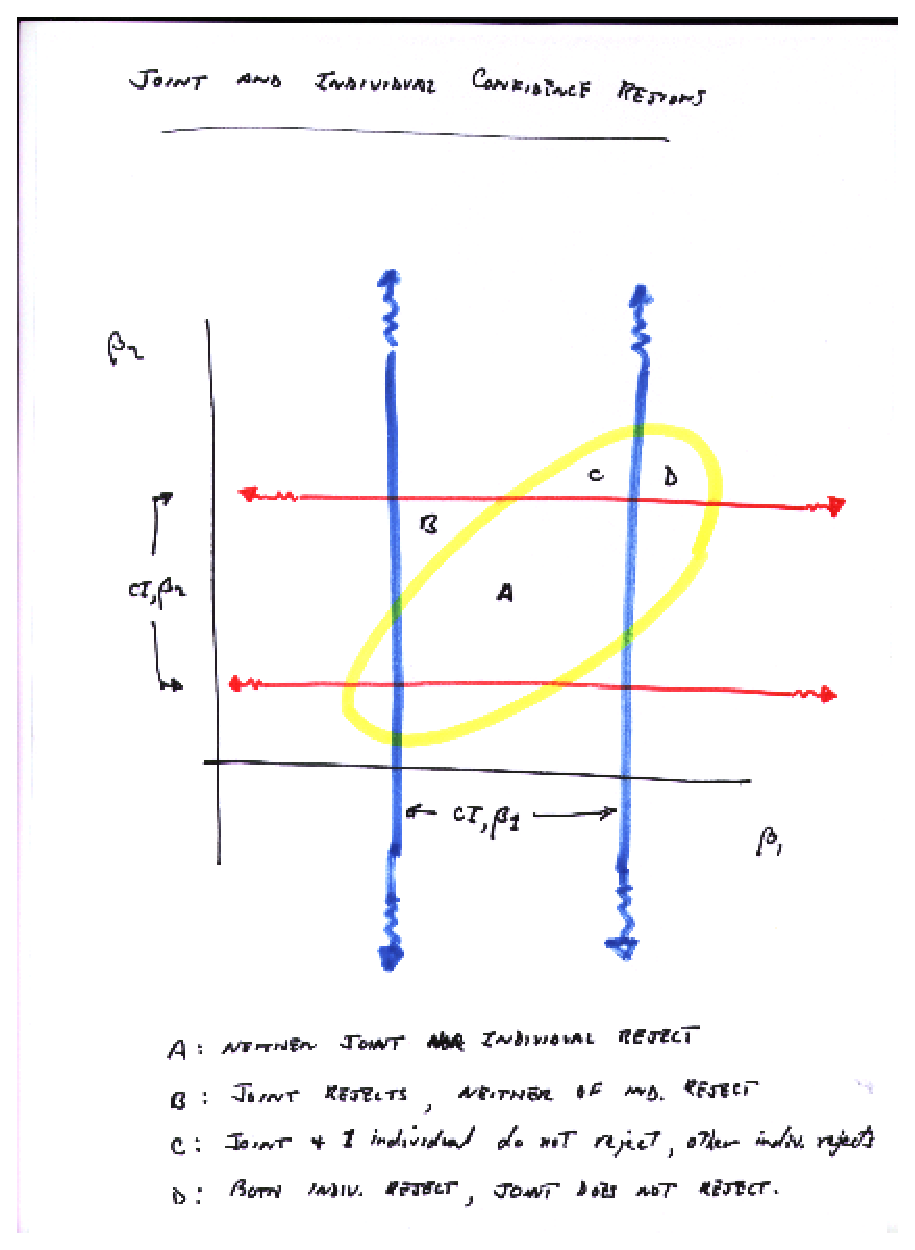
\includegraphics{/home/michael/Mystuff/Econometrics/Examples/Figures/JointConfidenceRegion}
\end{figure}

\begin{itemize}
\item The region is an ellipse, since the CI for an individual coefficient defines a (infinitely long) rectangle with total prob. mass $1-\alpha,$ since the other coefficient is marginalized (e.g., can take on any value). Since the ellipse is bounded in both dimensions but also contains mass $1-\alpha,$ it must extend beyond the bounds of the individual CI.
\item From the pictue we can see that:

\begin{itemize}
\item Rejection of hypotheses individually does not imply that the joint test will reject.
\item Joint rejection does not imply individal tests will reject. 
\end{itemize}
\end{itemize}

\section{Bootstrapping}

When we rely on asymptotic theory to use the normal distribution-based tests and confidence intervals, we're often at serious risk of making important errors. If the sample size is small and errors are highly nonnormal, the small sample distribution of $\sqrt{n}\left(\hat{\beta}-\beta_{0}\right)$ may be very different than its large sample distribution. Also, the distributions of test statistics may not resemble their limiting distributions at all. A means of trying to gain information on the small sample distribution of test statistics and estimators is the \emph{bootstrap.} We'll consider a simple example, just to get the main idea.

Suppose that 
\begin{eqnarray*}
y & = & X\beta_{0}+\varepsilon\\
\varepsilon & \sim & IID(0,\sigma_{0}^{2})\\
 & X\textrm{ is nonstochastic}
\end{eqnarray*}
 Given that the distribution of $\varepsilon$ is unknown, the distribution of $\hat{\beta}$ will be unknown in small samples. However, since we have random sampling, we could generate \emph{artificial data.} The steps are:
\begin{enumerate}
\item Draw $n$ observations from $\hat{\varepsilon}$ \textbf{with replacement}. Call this vector $\tilde{\varepsilon}^{j}$ (it's a $n\times1).$
\item Then generate the data by $\tilde{y}^{j}=X\hat{\beta}+\tilde{\varepsilon}^{j}$
\item Now take this and estimate 
\[
\tilde{\beta}^{j}=(X^{\prime}X)^{-1}X^{\prime}\tilde{y}^{j}.
\]

\item Save $\tilde{\beta}^{j}$
\item Repeat steps 1-4, until we have a large number, $J,$ of $\tilde{\beta}^{j}.$
\end{enumerate}
With this, we can use the replications to calculate the \emph{empirical distribution of} $\tilde{\beta}_{j}.$ One way to form a 100(1-$\alpha)\%$ confidence interval for $\beta_{0}$ would be to order the $\tilde{\beta}^{j}$ from smallest to largest, and drop the first and last $J\alpha/2$ of the replications, and use the remaining endpoints as the limits of the CI. Note that this will not give the shortest CI if the empirical distribution is skewed.
\begin{itemize}
\item Suppose one was interested in the distribution of some function of $\hat{\beta},$ for example a test statistic. Simple: just calculate the transformation for each $j,$ and work with the empirical distribution of the transformation.
\item If the assumption of iid errors is too strong (for example if there is heteroscedasticity or autocorrelation, see below) one can work with a bootstrap defined by sampling from $(y,x)$ with replacement.
\item How to choose $J$: $J$ should be large enough that the results don't change with repetition of the entire bootstrap. This is easy to check. If you find the results change a lot, increase $J$ and try again.
\item The bootstrap is based fundamentally on the idea that the empirical distribution of the sample data converges to the actual sampling distribution as $n$ becomes large, so statistics based on sampling from the empirical distribution should converge in distribution to statistics based on sampling from the actual sampling distribution.
\item In finite samples, this doesn't hold. At a minimum, the bootstrap is a good way to check if asymptotic theory results offer a decent approximation to the small sample distribution.
\item Bootstrapping can be used to test hypotheses. Basically, use the bootstrap to get an approximation to the empirical distribution of the test statistic under the alternative hypothesis, and use this to get critical values. Compare the test statistic calculated using the real data, under the null, to the bootstrap critical values. There are many variations on this theme, which we won't go into here. 
\end{itemize}

\section{Wald test for nonlinear restrictions: the delta method}

Testing nonlinear restrictions of a linear model is not much more difficult, at least when the model is linear. Since estimation subject to nonlinear restrictions requires nonlinear estimation methods, which are beyond the score of this course, we'll just consider the Wald test for nonlinear restrictions on a linear model.

Consider the $q$ nonlinear restrictions 
\[
r(\beta_{0})=0.
\]
 where $r(\cdot)\;$ is a $q$-vector valued function. Write the derivative of the restriction evaluated at $\beta$ as 
\[
\left.D_{\beta^{\prime}}r(\beta)\right|_{\beta}=R(\beta)
\]
 We suppose that the restrictions are not redundant in a neighborhood of $\beta_{0}$, so that 
\[
\rho(R(\beta))=q
\]
 in a neighborhood of $\beta_{0}.$ Take a first order Taylor's series expansion of $r(\hat{\beta})$ about $\beta_{0}$: 
\[
r(\hat{\beta})=r(\beta_{0})+R(\beta^{*})(\hat{\beta}-\beta_{0})
\]
 where $\beta^{*}$ is a convex combination of $\hat{\beta}$ and $\beta_{0}.$ Under the null hypothesis we have 
\[
r(\hat{\beta})=R(\beta^{*})(\hat{\beta}-\beta_{0})
\]
 Due to consistency of $\hat{\beta}$ we can replace $\beta^{*}$ by $\beta_{0}$, asymptotically, so 
\[
\sqrt{n}r(\hat{\beta})\overset{a}{=}\sqrt{n}R(\beta_{0})(\hat{\beta}-\beta_{0})
\]
 We've already seen the distribution of $\sqrt{n}(\hat{\beta}-\beta_{0}).$ Using this we get 
\[
\sqrt{n}r(\hat{\beta})\overset{d}{\rightarrow}N\left(0,R(\beta_{0})Q_{X}^{-1}R(\beta_{0})^{\prime}\sigma_{0}^{2}\right).
\]
 Considering the quadratic form 
\[
\frac{nr(\hat{\beta})^{\prime}\left(R(\beta_{0})Q_{X}^{-1}R(\beta_{0})^{\prime}\right)^{-1}r(\hat{\beta})}{\sigma_{0}^{2}}\overset{d}{\rightarrow}\chi^{2}(q)
\]
 under the null hypothesis. Substituting consistent estimators for $\beta_{0,}Q_{X}$ and $\sigma_{0}^{2},$ the resulting statistic is 
\[
\frac{r(\hat{\beta})^{\prime}\left(R(\hat{\beta})(X^{\prime}X)^{-1}R(\hat{\beta})^{\prime}\right)^{-1}r(\hat{\beta})}{\widehat{\sigma^{2}}}\overset{d}{\rightarrow}\chi^{2}(q)
\]
 under the null hypothesis.
\begin{itemize}
\item This is known in the literature as the \emph{delta method}, or as \emph{Klein's approximation}.
\item Since this is a Wald test, it will tend to over-reject in finite samples. The score and LR tests are also possibilities, but they require estimation methods for nonlinear models, which aren't in the scope of this course. 
\end{itemize}
Note that this also gives a convenient way to estimate nonlinear functions and associated asymptotic confidence intervals. If the nonlinear function $r(\beta_{0})$ is not hypothesized to be zero, we just have 
\[
\sqrt{n}\left(r(\hat{\beta})-r(\beta_{0})\right)\overset{d}{\rightarrow}N\left(0,R(\beta_{0})Q_{X}^{-1}R(\beta_{0})^{\prime}\sigma_{0}^{2}\right)
\]
 so an approximation to the distribution of the function of the estimator is 
\[
r(\hat{\beta})\approx N(r(\beta_{0}),R(\beta_{0})(X^{\prime}X)^{-1}R(\beta_{0})^{\prime}\sigma_{0}^{2})
\]
 For example, the vector of elasticities of a function $f(x)$ is 
\[
\eta(x)=\frac{\partial f(x)}{\partial x}\odot\frac{x}{f(x)}
\]
where $\odot$ means element-by-element multiplication. Suppose we estimate a linear function 
\[
y=x^{\prime}\beta+\varepsilon.
\]
 The elasticities of $y$ w.r.t. $x$ are 
\[
\eta(x)=\frac{\beta}{x^{\prime}\beta}\odot x
\]
(note that this is the entire vector of elasticities). The estimated elasticities are 
\[
\widehat{\eta}(x)=\frac{\hat{\beta}}{x^{\prime}\hat{\beta}}\odot x
\]
 To calculate the estimated standard errors of all five elasticites, use 
\begin{eqnarray*}
R(\beta) & = & \frac{\partial\eta(x)}{\partial\beta^{\prime}}\\
 & = & \frac{\left[\begin{array}{cccc}
x_{1} & 0 & \cdots & 0\\
0 & x_{2} &  & \vdots\\
\vdots &  & \ddots & 0\\
0 & \cdots & 0 & x_{k}
\end{array}\right]x'\beta-\left[\begin{array}{cccc}
\beta_{1}x_{1}^{2} & 0 & \cdots & 0\\
0 & \beta_{2}x_{2}^{2} &  & \vdots\\
\vdots &  & \ddots & 0\\
0 & \cdots & 0 & \beta_{k}x_{k}^{2}
\end{array}\right]}{(x'\beta)^{2}}.
\end{eqnarray*}
To get a consistent estimator just substitute in $\hat{\beta}$. Note that the elasticity and the standard error are functions of $x.$ The program  \htmladdnormallink{ExampleDeltaMethod.m}{file:///home/michael/Mystuff/Econometrics/Examples/Restrictions/ExampleDeltaMethod.m} shows how this can be done. 

In many cases, nonlinear restrictions can also involve the data, not just the parameters. For example, consider a model of expenditure shares. Let $x(p,m)$ be a demand funcion, where $p$ is prices and $m$ is income. An expenditure share system for $G$ goods is 
\[
s_{i}(p,m)=\frac{p_{i}x_{i}(p,m)}{m},i=1,2,...,G.
\]
 Now demand must be positive, and we assume that expenditures sum to income, so we have the restrictions 
\begin{eqnarray*}
0 & \leq s_{i}(p,m)\leq1, & \forall i\\
\sum_{i=1}^{G}s_{i}(p,m) & = & 1
\end{eqnarray*}
 Suppose we postulate a linear model for the expenditure shares: 
\[
s_{i}(p,m)=\beta_{1}^{i}+p^{\prime}\beta_{p}^{i}+m\beta_{m}^{i}+\varepsilon^{i}
\]
 It is fairly easy to write restrictions such that the shares sum to one, but the restriction that the shares lie in the $[0,1]$ interval depends on both parameters and the values of $p$ and $m.$ It is impossible to impose the restriction that $0\leq s_{i}(p,m)\leq1$ for all possible $p$ and $m.$ In such cases, one might consider whether or not a linear model is a reasonable specification.


\section{\label{sec:Example: Nerlove restrictions}Example: the Nerlove data}

Remember that we in a previous example (section \ref{sub:The-Nerlove-data}) that the OLS results for the Nerlove model are 

\begin{singlespace}
\verbatiminput{Examples/OLS/nerlove.out}
\end{singlespace}

Note that $s_{K}=\beta_{K}<0$, and that $\beta_{L}+\beta_{F}+\beta_{K}\neq1$.

Remember that if we have constant returns to scale, then $\beta_{Q}=1,$ and if there is homogeneity of degree 1 then $\beta_{L}+\beta_{F}+\beta_{K}=1$. We can test these hypotheses either separately or jointly.  \htmladdnormallink{NerloveRestrictions.m}{file:///home/michael/Mystuff/Econometrics/Examples/Restrictions/NerloveRestrictions.m}  imposes and tests CRTS and then HOD1. From it we obtain the results that follow: 

\verbatiminput{Examples/Restrictions/NerloveRestrictions.out}

Notice that the input price coefficients in fact sum to 1 when HOD1 is imposed. HOD1 is not rejected at usual significance levels (\emph{e.g., $\alpha=0.10$}). Also, $R^{2}$ does not drop much when the restriction is imposed, compared to the unrestricted results. For CRTS, you should note that $\beta_{Q}=1$, so the restriction is satisfied. Also note that the hypothesis that $\beta_{Q}=1$ is rejected by the test statistics at all reasonable significance levels. Note that $R^{2}$ drops quite a bit when imposing CRTS. If you look at the unrestricted estimation results, you can see that a t-test for $\beta_{Q}=1$ also rejects, and that a confidence interval for $\beta_{Q}$ does not overlap 1. 

From the point of view of neoclassical economic theory, these results are not anomalous: HOD1 is an implication of the theory, but CRTS is not.
\begin{xca}
Modify the NerloveRestrictions.m program to impose and test the restrictions jointly.
\end{xca}

\paragraph{\label{Chow test}The Chow test}

Since CRTS is rejected, let's examine the possibilities more carefully. Recall that the data is sorted by output (the third column). Define 5 subsamples of firms, with the first group being the 29 firms with the lowest output levels, then the next 29 firms, etc. The five subsamples can be indexed by $j=1,2,...,5,$ where $j=1$ for $t=1,2,...29$, $j=2$ for $t=30,31,...58$, etc. Define \emph{dummy variables} $D_{1},D_{2},...,D_{5}$ where
\begin{align*}
D_{1} & =\begin{cases}
1 & t\in\{1,2,...29\}\\
0 & t\notin\{1,2,...29\}
\end{cases}\\
D_{2} & =\begin{cases}
1 & t\in\{30,31,...58\}\\
0 & t\notin\{30,31,...58\}
\end{cases}\\
\vdots\\
D_{5} & =\begin{cases}
1 & t\in\{117,118,...,145\}\\
0 & t\notin\{117,118,...,145\}
\end{cases}
\end{align*}
 Define the model
\begin{equation}
\ln C_{t}=\sum_{j=1}^{5}\alpha_{1}D_{j}+\sum_{j=1}^{5}\gamma_{j}D_{j}\ln Q_{t}+\sum_{j=1}^{5}\beta_{Lj}D_{j}\ln P_{Lt}+\sum_{j=1}^{5}\beta_{Fj}D_{j}\ln P_{Ft}+\sum_{j=1}^{5}\beta_{Kj}D_{j}\ln P_{Kt}+\epsilon_{t}
\end{equation}
Note that the first column of nerlove.data indicates this way of breaking up the sample, and provides and easy way of defining the dummy variables. The new model may be written as
\begin{equation}
\left[\begin{array}{l}
y_{1}\\
y_{2}\\
\vdots\\
\\
y_{5}
\end{array}\right]=\left[\begin{array}{lllll}
X_{1} & 0 & \cdots &  & 0\\
0 & X_{2}\\
\vdots &  & X_{3}\\
 &  &  & X_{4} & 0\\
0 &  &  &  & X_{5}
\end{array}\right]\left[\begin{array}{l}
\beta^{1}\\
\beta^{2}\\
\\
\\
\beta^{5}
\end{array}\right]+\left[\begin{array}{l}
\epsilon^{1}\\
\epsilon^{2}\\
\vdots\\
\\
\epsilon^{5}
\end{array}\right]\label{nerlove - all coefficients vary}
\end{equation}
 where $y_{1}$ is 29$\times1,$ $X_{1}$ is 29$\times5,$ $\beta^{j}$ is the $5\times1$ vector of coefficients for the $j^{th}$ subsample (e.g., $\beta^{1}=\mbox{\ensuremath{\left(\alpha_{1},\gamma_{1},\beta_{L1},\beta_{F1},\beta_{K1}\right)}\ensuremath{\ensuremath{^{\prime}}}}$), and $\epsilon^{j}$ is the $29\times1$ vector of errors for the $j^{th}$ subsample.

The Octave program  \htmladdnormallink{Restrictions/ChowTest.m}{file:///home/michael/Mystuff/Econometrics/Examples/Restrictions/ChowTest.m} estimates the above model. It also tests the hypothesis that the five subsamples share the same parameter vector, or in other words, that there is coefficient stability across the five subsamples. The null to test is that the parameter vectors for the separate groups are all the same, that is,
\[
\beta^{1}=\beta^{2}=\beta^{3}=\beta^{4}=\beta^{5}
\]
 This type of test, that parameters are constant across different sets of data, is sometimes referred to as a \emph{Chow} \emph{test.}
\begin{itemize}
\item There are 20 restrictions. If that's not clear to you, look at the Octave program.
\item The restrictions are rejected at all conventional significance levels.
\end{itemize}
Since the restrictions are rejected, we should probably use the unrestricted model for analysis. What is the pattern of RTS\ as a function of the output group (small to large)? Figure \ref{Nerlove RTS} plots RTS. We can see that there is increasing RTS for small firms, but that RTS is approximately constant for large firms. 

\begin{figure}
\caption{\label{Nerlove RTS}RTS as a function of firm size}


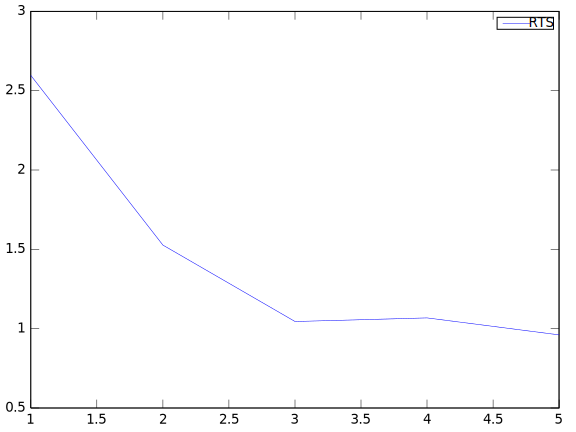
\includegraphics{Examples/Restrictions/rts}
\end{figure}



\section{Exercises}
\begin{enumerate}
\item Using the Chow test on the Nerlove model, we reject that there is coefficient stability across the 5 groups. But perhaps we could restrict the input price coefficients to be the same but let the constant and output coefficients vary by group size. This new model is
\begin{equation}
\ln C=\sum_{j=1}^{5}\alpha_{j}D_{j}+\sum_{j=1}^{5}\gamma_{j}D_{j}\ln Q+\beta_{L}\ln P_{L}+\beta_{F}\ln P_{F}+\beta_{K}\ln P_{K}+\epsilon\label{Nerlove, favorite model}
\end{equation}


\begin{enumerate}
\item estimate this model by OLS, giving $R^{2}$, estimated standard errors for coefficients, t-statistics for tests of significance, and the associated p-values. Interpret the results in detail.
\item Test the restrictions implied by this model (relative to the model that lets all coefficients vary across groups) using the F, qF, Wald, score and likelihood ratio tests. Comment on the results.
\item Estimate this model but imposing the HOD1 restriction, \emph{using an OLS} estimation program. Don't use mc\_olsr or any other restricted OLS estimation program. Give estimated standard errors for all coefficients.
\item Plot the estimated RTS parameters as a function of firm size. Compare the plot to that given in the notes for the unrestricted model. Comment on the results.
\end{enumerate}
\item For the model of the above question, compute 95\% confidence intervals for RTS for each of the 5 groups of firms, using the delta method to compute standard errors. Comment on the results.
\item Perform a Monte Carlo study that generates data from the model 
\[
y=-2+1x_{2}+1x_{3}+\epsilon
\]
where the sample size is 30, $x_{2}$ and $x_{3}$ are independently uniformly distributed on $[0,1]$ and $\epsilon\sim IIN(0,1)$

\begin{enumerate}
\item Compare the means and standard errors of the estimated coefficients using OLS and restricted OLS, imposing the restriction that $\beta_{2}+\beta_{3}=2.$
\item Compare the means and standard errors of the estimated coefficients using OLS and restricted OLS, imposing the restriction that $\beta_{2}+\beta_{3}=1.$
\item Discuss the results.
\end{enumerate}

\newpage{}

\end{enumerate}

\chapter{\label{cha:Stochastic-regressors}Stochastic regressors}

Up to now we have treated the regressors as fixed, which is clearly unrealistic. Now we will assume they are random. There are several ways to think of the problem. First, if we are interested in an analysis \emph{conditional} on the explanatory variables, then it is irrelevant if they are stochastic or not, since conditional on the values of they regressors take on, they are nonstochastic, which is the case already considered.
\begin{itemize}
\item In cross-sectional analysis it is usually reasonable to make the analysis conditional on the regressors.
\item In dynamic models, where $y_{t}$ may depend on $y_{t-1},$ a conditional analysis is not sufficiently general, since we may want to predict into the future many periods out, so we need to consider the behavior of $\hat{\beta}$ and the relevant test statistics unconditional on $X.$
\end{itemize}
The model we'll deal will involve a combination of the following assumptions
\begin{assumption}
\textbf{Linearity}: the model is a linear function of the parameter vector $\beta_{0}:$
\[
y_{t}=x_{t}^{\prime}\beta_{0}+\varepsilon_{t},
\]
 or in matrix form, 
\[
y=X\beta_{0}+\varepsilon,
\]
 where $y$ is $n\times1,$ $X=\left(\begin{array}{cccc}
x_{1} & x_{2} & \cdots & x_{n}\end{array}\right)^{\prime},$ where $x_{t}$ is $K\times1,$ and $\beta_{0}$ and $\varepsilon$ are conformable.
\end{assumption}
$\,$
\begin{assumption}
\textbf{Stochastic, linearly independent regressors}

$X$ has rank $K$ with probability 1

$X$ is stochastic

$\lim_{n\rightarrow\infty}\Pr\left(\frac{1}{n}X^{\prime}X=Q_{X}\right)=1,$ where $Q_{X}$ is a finite positive definite matrix.
\end{assumption}
$\,$
\begin{assumption}
\textbf{Central limit theorem}

$n^{-1/2}X^{\prime}\varepsilon\overset{d}{\rightarrow}N(0,Q_{X}\sigma_{0}^{2})$
\end{assumption}
$\,$
\begin{assumption}
\textbf{Normality (Optional)}: $\varepsilon|X\sim N(0,\sigma^{2}I_{n})$: $\epsilon$ is normally distributed 
\end{assumption}
$\,$
\begin{assumption}
\textbf{Strongly exogenous} \textbf{regressors}. The regressors $\mathbf{X}$ are strongly exogenous if 
\begin{eqnarray}
\mathcal{E}(\varepsilon_{t}|\mathbf{X}) & = & 0,\forall t\label{assumption: strong exogeneity}
\end{eqnarray}

\end{assumption}
$\,$
\begin{assumption}
\textbf{\label{ass:Weakly-exogenous-regressors:}Weakly exogenous regressors}: The regressors are weakly exogenous if 
\begin{eqnarray*}
\mathcal{E}(\varepsilon_{t}|\mathbf{x}_{t}) & = & 0,\forall t
\end{eqnarray*}

\end{assumption}
In both cases, $\mathbf{x}_{t}^{\prime}\beta$ is the conditional mean of $y_{t}$ given $\mathbf{x}_{t}$: $E(y_{t}|\mathbf{x}_{t})=\mathbf{x}_{t}^{\prime}\beta$


\section{Case 1}

\emph{Normality of} $\varepsilon,$ strongly exogenous regressors

In this case, 
\[
\hat{\beta}=\beta_{0}+(X^{\prime}X)^{-1}X^{\prime}\varepsilon
\]
 
\begin{eqnarray*}
\mathcal{E}(\hat{\beta}|X) & = & \beta_{0}+(X^{\prime}X)^{-1}X^{\prime}\mathcal{E}(\varepsilon|X)\\
 & = & \beta_{0}
\end{eqnarray*}
 and since this holds for all $X,$ $E(\hat{\beta})=\beta$, unconditional on $X.$ Likewise,
\[
\hat{\beta}|X\sim N\left(\beta,(X^{\prime}X)^{-1}\sigma_{0}^{2}\right)
\]

\begin{itemize}
\item If the density of $X$ is $d\mu(X),$ the marginal density of $\hat{\beta}$ is obtained by multiplying the conditional density by $d\mu(X)$ and integrating over $X.$ Doing this leads to a nonnormal density for $\hat{\beta},$ in small samples.
\item However, conditional on $X,$ the usual test statistics have the $t,$ $F$ and $\chi^{2}$ distributions. \emph{Importantly,} these distributions don't depend on $X,$ so when marginalizing to obtain the unconditional distribution, nothing changes. The tests are valid in small samples.
\item Summary: When $X$ is stochastic but strongly exogenous and $\varepsilon$ is normally distributed:

\begin{enumerate}
\item $\hat{\beta}$ is unbiased
\item $\hat{\beta}$ is nonnormally distributed
\item The usual test statistics have the same distribution as with nonstochastic $X.$
\item The Gauss-Markov theorem still holds, since it holds conditionally on $X,$ and this is true for all $X.$
\item Asymptotic properties are treated in the next section. 
\end{enumerate}
\end{itemize}

\section{Case 2}

$\varepsilon$\emph{\ nonnormally distributed, strongly exogenous regressors}

The unbiasedness of $\hat{\beta}$ carries through as before. However, the argument regarding test statistics doesn't hold, due to nonnormality of $\varepsilon.$ Still, we have 
\begin{eqnarray*}
\hat{\beta} & = & \beta_{0}+(X^{\prime}X)^{-1}X^{\prime}\varepsilon\\
 & = & \beta_{0}+\left(\frac{X^{\prime}X}{n}\right)^{-1}\frac{X^{\prime}\varepsilon}{n}
\end{eqnarray*}
 Now 
\[
\left(\frac{X^{\prime}X}{n}\right)^{-1}\overset{p}{\rightarrow}Q_{X}^{-1}
\]
 by assumption, and 
\[
\frac{X^{\prime}\varepsilon}{n}=\frac{n^{-1/2}X^{\prime}\varepsilon}{\sqrt{n}}\overset{p}{\rightarrow}0
\]
 since the numerator converges to a $N(0,Q_{X}\sigma^{2})$ r.v. and the denominator still goes to infinity. We have unbiasedness and the variance disappearing, so, \emph{the estimator is consistent}: 
\[
\hat{\beta}\overset{p}{\rightarrow}\beta_{0}.
\]


Considering the asymptotic distribution 
\begin{eqnarray*}
\sqrt{n}\left(\hat{\beta}-\beta_{0}\right) & = & \sqrt{n}\left(\frac{X^{\prime}X}{n}\right)^{-1}\frac{X^{\prime}\varepsilon}{n}\\
 & = & \left(\frac{X^{\prime}X}{n}\right)^{-1}n^{-1/2}X^{\prime}\varepsilon
\end{eqnarray*}
 so 
\[
\sqrt{n}\left(\hat{\beta}-\beta_{0}\right)\overset{d}{\rightarrow}N(0,Q_{X}^{-1}\sigma_{0}^{2})
\]
 directly following the assumptions. \emph{Asymptotic normality of the estimator still holds.} Since the asymptotic results on all test statistics only require this, all the previous asymptotic results on test statistics are also valid in this case.
\begin{itemize}
\item Summary: Under strongly exogenous regressors, with $\varepsilon$ normal or nonnormal, $\hat{\beta}$ has the properties:

\begin{enumerate}
\item Unbiasedness
\item Consistency
\item Gauss-Markov theorem holds, since it holds in the previous case and doesn't depend on normality.
\item Asymptotic normality
\item Tests are asymptotically valid
\item Tests are not valid in small samples if the error is normally distributed
\end{enumerate}
\end{itemize}

\section{Case 3}

\emph{Weakly exogenous regressors}

An important class of models are \emph{dynamic models}, where lagged dependent variables have an impact on the current value. A simple version of these models that captures the important points is 
\begin{eqnarray*}
y_{t} & = & z_{t}^{\prime}\alpha+\sum_{s=1}^{p}\gamma_{s}y_{t-s}+\varepsilon_{t}\\
 & = & x_{t}^{\prime}\beta+\varepsilon_{t}
\end{eqnarray*}
 where now $x_{t}$ contains lagged dependent variables. Clearly, even with $E(\epsilon_{t}|\mathbf{x}_{t})=0,$ $X$ and $\varepsilon$ are not uncorrelated, so one can't show unbiasedness. For example, 
\[
\mathcal{E}(\varepsilon_{t-1}x_{t})\neq0
\]
 since $x_{t}$ contains $y_{t-1}$ (which is a function of $\varepsilon_{t-1})$ as an element.
\begin{itemize}
\item This fact implies that all of the small sample properties such as unbiasedness, Gauss-Markov theorem, and small sample validity of test statistics \emph{do not hold} in this case. Recall Figure \ref{figure-biasedness}. This is a case of weakly exogenous regressors, and we see that the OLS estimator is biased in this case.
\item Nevertheless, under the above assumptions, all asymptotic properties continue to hold, using the same arguments as before.
\end{itemize}

\section{When are the assumptions reasonable?}

The two assumptions we've added are
\begin{enumerate}
\item $\lim_{n\rightarrow\infty}\Pr\left(\frac{1}{n}X^{\prime}X=Q_{X}\right)=1,$ a $Q_{X}$ finite positive definite matrix.
\item $n^{-1/2}X^{\prime}\varepsilon\overset{d}{\rightarrow}N(0,Q_{X}\sigma_{0}^{2})$
\end{enumerate}
The most complicated case is that of dynamic models, since the other cases can be treated as nested in this case. There exist a number of central limit theorems for dependent processes, many of which are fairly technical. We won't enter into details (see Hamilton, Chapter 7 if you're interested). A main requirement for use of standard asymptotics for a dependent sequence 
\[
\{s_{t}\}=\{\frac{1}{n}\sum_{t=1}^{n}z_{t}\}
\]
 to converge in probability to a finite limit is that $z_{t}$ be \emph{stationary}, in some sense.
\begin{itemize}
\item Strong stationarity requires that the joint distribution of the set 
\[
\{z_{t},z_{t+s},z_{t-q},...\}
\]
 not depend on $t.$
\item Covariance (weak) stationarity requires that the first and second moments of this set not depend on $t.$
\item An example of a sequence that doesn't satisfy this is an AR(1) process with a unit root (a \emph{random walk)}: 
\begin{eqnarray*}
x_{t} & = & x_{t-1}+\varepsilon_{t}\\
\varepsilon_{t} & \sim & IIN(0,\sigma^{2})
\end{eqnarray*}
 One can show that the variance of $x_{t}$ depends upon $t$ in this case, so it's not weakly stationary.
\item The series $\sin t+\epsilon_{t}$ has a first moment that depends upon $t$, so it's not weakly stationary either.
\end{itemize}
Stationarity prevents the process from trending off to plus or minus infinity, and prevents cyclical behavior which would allow correlations between far removed $z_{t}$ znd $z_{s}$ to be high. \emph{Draw a picture here.}
\begin{itemize}
\item In summary, the assumptions are reasonable when the stochastic conditioning variables have variances that are finite, and are not too strongly dependent. The AR(1) model with unit root is an example of a case where the dependence is too strong for standard asymptotics to apply.
\item The study of nonstationary processes is an important part of econometrics, but it isn't in the scope of this course. 
\end{itemize}

\section{Exercises}
\begin{enumerate}
\item Show that for two random variables $A$ and $B,$ if $E(A|B)=0,$ then $E\left(Af(B)\right)=0$. How is this used in the proof of the Gauss-Markov theorem?
\item Is it possible for an AR(1) model for time series data, \emph{e.g.,} $y_{t}=0+0.9y_{t-1}+\varepsilon_{t}$ satisfy weak exogeneity? Strong exogeneity? Discuss.\newpage{}
\end{enumerate}

\chapter{Data problems}

In this section we'll consider problems associated with the regressor matrix: collinearity, missing observations and measurement error.


\section{Collinearity}


\subsection{Motivation: Data on Mortality and Related Factors\label{sec:Motivation:-Data-on}}

The data set  \htmladdnormallink{mortality.data}{file:///home/michael/Mystuff/Econometrics/Examples/Data/mortality.data}  contains annual data from 1947 - 1980 on death rates in the U.S., along with data on factors like smoking and consumption of alcohol. The data description is:

DATA4-7: Death rates in the U.S. due to coronary heart disease and their

determinants. Data compiled by Jennifer Whisenand
\begin{itemize}
\item chd = death rate per 100,000 population (Range 321.2 - 375.4)
\item cal = Per capita consumption of calcium per day in grams (Range 0.9 - 1.06)
\item unemp = Percent of civilian labor force unemployed in 1,000 of persons 16 years and older (Range 2.9 - 8.5)
\item cig = Per capita consumption of cigarettes in pounds of tobacco by persons 18 years and older--approx. 339 cigarettes per pound of tobacco (Range 6.75 - 10.46)
\item edfat = Per capita intake of edible fats and oil in pounds--includes lard, margarine and butter (Range 42 - 56.5)
\item meat = Per capita intake of meat in pounds--includes beef, veal, pork, lamb and mutton (Range 138 - 194.8)
\item spirits = Per capita consumption of distilled spirits in taxed gallons for individuals 18 and older (Range 1 - 2.9)
\item beer = Per capita consumption of malted liquor in taxed gallons for individuals 18 and older (Range 15.04 - 34.9)
\item wine = Per capita consumption of wine measured in taxed gallons for individuals 18 and older (Range 0.77 - 2.65)
\end{itemize}
\newpage{}Consider estimation results for several models:


\thispagestyle{empty}

%%% the following needs the amsmath LaTeX package

\begin{gather}
\begin{split}
\widehat{\rm chd} &= 
\underset{(58.939)}{334.914}
+\underset{(5.156)}{5.41216}\,\mbox{cig}
+\underset{(7.373)}{36.8783}\,\mbox{spirits}
-\underset{(1.2513)}{5.10365}\,\mbox{beer}\\
& +\underset{(12.735)}{13.9764}\,\mbox{wine}
\end{split}
 \notag \\
T = 34 \quad \bar{R}^2 = 0.5528 \quad F(4,29) = 11.2 \quad \hat{\sigma} = 9.9945\notag \\
\centerline{(standard errors in parentheses)} \notag
\end{gather}




\thispagestyle{empty}

%%% the following needs the amsmath LaTeX package

\begin{gather}
\widehat{\rm chd} = 
\underset{(56.624)}{353.581}
+\underset{(4.7523)}{3.17560}\,\mbox{cig}
+\underset{(7.275)}{38.3481}\,\mbox{spirits}
-\underset{(1.0102)}{4.28816}\,\mbox{beer}
 \notag \\
T = 34 \quad \bar{R}^2 = 0.5498 \quad F(3,30) = 14.433 \quad \hat{\sigma} = 10.028\notag \\
\centerline{(standard errors in parentheses)} \notag
\end{gather}



\thispagestyle{empty}

%%% the following needs the amsmath LaTeX package

\begin{gather}
\widehat{\rm chd} = 
\underset{(67.21)}{243.310}
+\underset{(6.1508)}{10.7535}\,\mbox{cig}
+\underset{(8.0359)}{22.8012}\,\mbox{spirits}
-\underset{(12.638)}{16.8689}\,\mbox{wine}
 \notag \\
T = 34 \quad \bar{R}^2 = 0.3198 \quad F(3,30) = 6.1709 \quad \hat{\sigma} = 12.327\notag \\
\centerline{(standard errors in parentheses)} \notag
\end{gather}




\thispagestyle{empty}

%%% the following needs the amsmath LaTeX package

\begin{gather}
\widehat{\rm chd} = 
\underset{(49.119)}{181.219}
+\underset{(4.4371)}{16.5146}\,\mbox{cig}
+\underset{(6.2079)}{15.8672}\,\mbox{spirits}
 \notag \\
T = 34 \quad \bar{R}^2 = 0.3026 \quad F(2,31) = 8.1598 \quad \hat{\sigma} = 12.481\notag \\
\centerline{(standard errors in parentheses)} \notag
\end{gather}


Note how the signs of the coefficients change depending on the model, and that the magnitudes of the parameter estimates vary a lot, too. The parameter estimates are highly sensitive to the particular model we estimate. Why? We'll see that the problem is that the data exhibit \emph{collinearity}.


\subsection{Collinearity: definition}

Collinearity is the existence of linear relationships amongst the regressors. We can always write 
\[
\lambda_{1}\mathbf{x}_{1}+\lambda_{2}\mathbf{x}_{2}+\cdots+\lambda_{K}\mathbf{x}_{K}+v=0
\]
 where $\mathbf{x}_{i}$ is the $i^{th}$ column of the regressor matrix $X,$ and $v$ is an $n\times1$ vector. In the case that there exists collinearity, the variation in $v$ is relatively small, so that there is an approximately exact linear relation between the regressors.
\begin{itemize}
\item ``relative'' and ``approximate'' are imprecise, so it's difficult to define when collinearilty exists. 
\end{itemize}
In the extreme, if there are exact linear relationships (every element of $v$ equal) then $\rho(X)<K,$ so $\rho(X^{\prime}X)<K,$ so $X^{\prime}X$ is not invertible and the OLS\ estimator is not uniquely defined. For example, if the model is 
\begin{eqnarray*}
y_{t} & = & \beta_{1}+\beta_{2}x_{2t}+\beta_{3}x_{3t}+\varepsilon_{t}\\
x_{2t} & = & \alpha_{1}+\alpha_{2}x_{3t}
\end{eqnarray*}
 then we can write 
\begin{eqnarray*}
y_{t} & = & \beta_{1}+\beta_{2}\left(\alpha_{1}+\alpha_{2}x_{3t}\right)+\beta_{3}x_{3t}+\varepsilon_{t}\\
 & = & \beta_{1}+\beta_{2}\alpha_{1}+\beta_{2}\alpha_{2}x_{3t}+\beta_{3}x_{3t}+\varepsilon_{t}\\
 & = & \left(\beta_{1}+\beta_{2}\alpha_{1}\right)+\left(\beta_{2}\alpha_{2}+\beta_{3}\right)x_{3t}\\
 & = & \gamma_{1}+\gamma_{2}x_{3t}+\varepsilon_{t}
\end{eqnarray*}

\begin{itemize}
\item The $\gamma^{\prime}s$ can be consistently estimated, but since the $\gamma^{\prime}$s define two equations in three $\beta^{\prime}s,$ the $\beta^{\prime}s$ can't be consistently estimated (there are multiple values of $\beta$ that solve the first order conditions). The $\beta^{\prime}s$ are \emph{unidentified} in the case of perfect collinearity.
\item Perfect collinearity is unusual, except in the case of an error in construction of the regressor matrix, such as including the same regressor twice. 
\end{itemize}
Another case where perfect collinearity may be encountered is with models with dummy variables, if one is not careful. Consider a model of rental price $(y_{i})$ of an apartment. This could depend factors such as size, quality etc., collected in $x_{i},$ as well as on the location of the apartment. Let $B_{i}=1$ if the $i^{th}$ apartment is in Barcelona, $B_{i}=0$ otherwise. Similarly, define $G_{i},$ $T_{i}$ and $L_{i}$ for Girona, Tarragona and Lleida. One could use a model such as 
\[
y_{i}=\beta_{1}+\beta_{2}B_{i}+\beta_{3}G_{i}+\beta_{4}T_{i}+\beta_{5}L_{i}+x_{i}^{\prime}\gamma+\varepsilon_{i}
\]
 In this model, $B_{i}+G_{i}+T_{i}+L_{i}=1,$ $\forall i,$ so there is an exact relationship between these variables and the column of ones corresponding to the constant. One must either drop the constant, or one of the qualitative variables.


\subsection{A brief aside on dummy variables}

\textbf{Dummy variable}: A dummy variable is a binary-valued variable that indicates whether or not some condition is true. It is customary to assign the value 1 if the condition is true, and 0 if the condition is false.

Dummy variables are used essentially like any other regressor. Use $d$ to indicate that a variable is a dummy, so that variables like $d_{t}$ and $d_{t2}$ are understood to be dummy variables. Variables like $x_{t}$ and $x_{t3}$ are ordinary continuous regressors. You know how to interpret the following models:

\[
y_{t}=\beta_{1}+\beta_{2}d_{t}+\epsilon_{t}
\]


\[
y_{t}=\beta_{1}d_{t}+\beta_{2}(1-d_{t})+\epsilon_{t}
\]


\[
y_{t}=\beta_{1}+\beta_{2}d_{t}+\beta_{3}x_{t}+\epsilon_{t}
\]
\textbf{Interaction terms:} an interaction term is the product of two variables, so that the effect of one variable on the dependent variable depends on the value of the other. The following model has an interaction term. Note that $\frac{\partial E(y|x)}{\partial x}=\beta_{3}+\beta_{4}d_{t}$. The slope depends on the value of $d_{t}$.

\[
y_{t}=\beta_{1}+\beta_{2}d_{t}+\beta_{3}x_{t}+\beta_{4}d_{t}x_{t}+\epsilon_{t}
\]
\textbf{Multiple dummy variables: }we can use more than one dummy variable in a model. We will study models of the form
\[
y_{t}=\beta_{1}+\beta_{2}d_{t1}+\beta_{3}d_{t2}+\beta_{4}x_{t}+\epsilon_{t}
\]


\[
y_{t}=\beta_{1}+\beta_{2}d_{t1}+\beta_{3}d_{t2}+\beta_{4}d_{t1}d_{t2}+\beta_{5}x_{t}+\epsilon_{t}
\]
\textbf{Incorrect usage: }You should understand why the following models are not correct usages of dummy variables:
\begin{enumerate}
\item overparameterization:
\[
y_{t}=\beta_{1}+\beta_{2}d_{t}+\beta_{3}(1-d_{t})+\epsilon_{t}
\]

\item multiple values assigned to multiple categories. Suppose that we a condition that defines 4 possible categories, and we create a variable $d=1$ if the observation is in the first category, $d=2$ if in the second, etc. (This is not strictly speaking a dummy variable, according to our definition). Why is the following model not a good one?
\[
y_{t}=\beta_{1}+\beta_{2}d+\epsilon
\]
What is the correct way to deal with this situation?
\end{enumerate}
\textbf{Multiple parameterizations. }To formulate a model that conditions on a given set of categorical information, there are multiple ways to use dummy variables. For example, the two models 
\[
y_{t}=\beta_{1}d_{t}+\beta_{2}(1-d_{t})+\beta_{3}x_{t}+\beta_{4}d_{t}x_{t}+\epsilon_{t}
\]
and

\[
y_{t}=\alpha_{1}+\alpha_{2}d_{t}+\alpha_{3}x_{t}d_{t}+\alpha_{4}x_{t}(1-d_{t})+\epsilon_{t}
\]
are equivalent. You should know what are the 4 equations that relate the $\beta_{j}$ parameters to the $\alpha_{j}$ parameters, $j=1,2,3,4.$ You should know how to interpret the parameters of both models.


\subsection{Back to collinearity}

The more common case, if one doesn't make mistakes such as these, is the existence of inexact linear relationships, \emph{i.e.}, correlations between the regressors that are less than one in absolute value, but not zero. The basic problem is that when two (or more) variables move together, it is difficult to determine their separate influences.
\begin{example}
Two children are in a room, along with a broken lamp. Both say ''I didn't do it!''. How can we tell who broke the lamp?
\end{example}
Lack of knowledge about the separate influences of variables is reflected in imprecise estimates, \emph{i.e}., estimates with high variances. \emph{With economic data, collinearity is commonly encountered, and is often a severe problem.}

When there is collinearity, the minimizing point of the objective function that defines the OLS estimator ($s(\beta)$, the sum of squared errors) is relatively poorly defined. This is seen in Figures \ref{nocollin} and \ref{collin}. 
\begin{figure}
\caption{\label{nocollin}$s(\beta)$ when there is no collinearity}


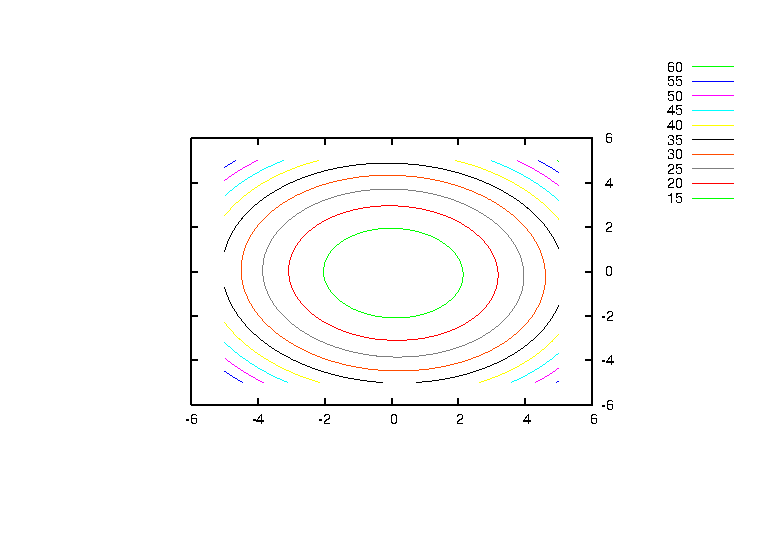
\includegraphics{Examples/Figures/nocollin}
\end{figure}


\begin{figure}
\caption{\label{collin}$s(\beta)$ when there is collinearity}


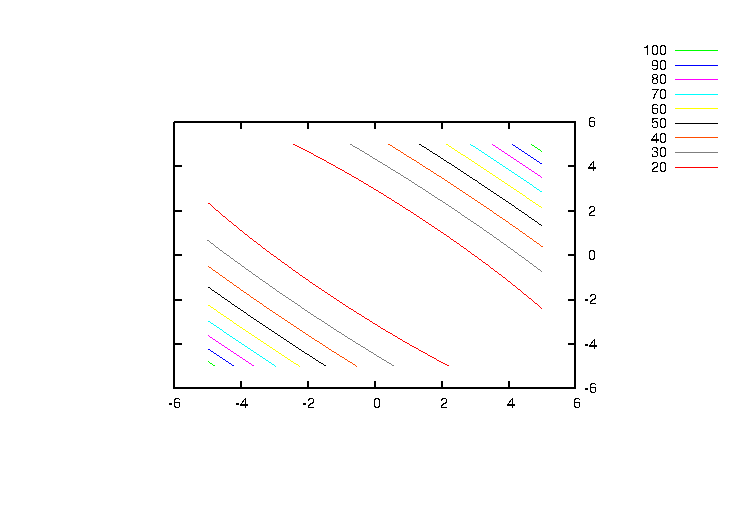
\includegraphics{Examples/Figures/collin}
\end{figure}


To see the effect of collinearity on variances, partition the regressor matrix as 
\[
X=\left[\begin{array}{cc}
\mathbf{x} & W\end{array}\right]
\]
 where $\mathbf{x}$ is the first column of $X$ (note:\ we can interchange the columns of $X$ isf we like, so there's no loss of generality in considering the first column). Now, the variance of $\hat{\beta},$ under the classical assumptions, is 
\[
V(\hat{\beta})=\left(X^{\prime}X\right)^{-1}\sigma^{2}
\]
 Using the partition, 
\[
X^{\prime}X=\left[\begin{array}{cc}
\mathbf{x}^{\prime}\mathbf{x} & \mathbf{x}^{\prime}W\\
W^{\prime}\mathbf{x} & W^{\prime}W
\end{array}\right]
\]
 and following a rule for partitioned inversion, 
\begin{eqnarray*}
\left(X^{\prime}X\right)_{1,1}^{-1} & = & \left(\mathbf{x}^{\prime}\mathbf{x}-\mathbf{x}^{\prime}W(W^{\prime}W)^{-1}W^{\prime}\mathbf{x}\right)^{-1}\\
 & = & \left(\mathbf{x}^{\prime}\left(I_{n}-W(W^{\prime}W)^{^{\prime}1}W^{\prime}\right)\mathbf{x}\right)^{-1}\\
 & = & \left(ESS_{\mathbf{x}|W}\right)^{-1}
\end{eqnarray*}
 where by $ESS_{\mathbf{x}|W}$ we mean the error sum of squares obtained from the regression 
\[
\mathbf{x}=W\lambda+v.
\]
 Since 
\[
R^{2}=1-ESS/TSS,
\]
 we have 
\[
ESS=TSS(1-R^{2})
\]
 so the variance of the coefficient corresponding to $\mathbf{x}$ is 
\begin{equation}
V(\hat{\beta}_{\mathbf{x}})=\frac{\sigma^{2}}{TSS_{\mathbf{x}}(1-R_{\mathbf{x}|W}^{2})}\label{eq:variance factors}
\end{equation}
 We see three factors influence the variance of this coefficient. It will be high if
\begin{enumerate}
\item $\sigma^{2}$ is large
\item There is little variation in $\mathbf{x}.$ \emph{Draw a picture here}.
\item There is a strong linear relationship between $x$ and the other regressors, so that $W$ can explain the movement in $\mathbf{x}$ well. In this case, $R_{\mathbf{x}|W}^{2}$ will be close to 1. As $R_{\mathbf{x}|W}^{2}\rightarrow1,V(\hat{\beta}_{\mathbf{x}})\rightarrow\infty.$
\end{enumerate}
The last of these cases is collinearity.

Intuitively, when there are strong linear relations between the regressors, it is difficult to determine the separate influence of the regressors on the dependent variable. This can be seen by comparing the OLS\ objective function in the case of no correlation between regressors with the objective function with correlation between the regressors. See the figures nocollin.ps (no correlation) and collin.ps (correlation), available on the web site.
\begin{example}
The Octave script  \htmladdnormallink{DataProblems/collinearity.m}{file:///home/michael/Mystuff/Econometrics/Examples/DataProblems/collinearity.m}  performs a Monte Carlo study with correlated regressors. The model is $y=1+x_{2}+x_{3}+\epsilon$, where the correlation between $x_{2}$ and $x_{3}$can be set. Three estimators are used: OLS, OLS dropping $x_{3}$ (a false restriction), and restricted LS using $\beta_{2}=\beta_{3}$ (a true restriction). The output when the correlation between the two regressors is 0.9 is\verbatiminput{Examples/DataProblems/collinearity.out}

Figure \ref{fig:Collinearity:-Monte-Carlo} shows histograms for the estimated $\beta_{2},$ for each of the three estimators.\end{example}
\begin{itemize}
\item repeat the experiment with a lower value of rho, and note how the standard errors of the OLS estimator change.
\end{itemize}
\begin{figure}
\caption{\label{fig:Collinearity:-Monte-Carlo}Collinearity: Monte Carlo results}


\subfloat[OLS,$\hat{\beta_{2}}$]{

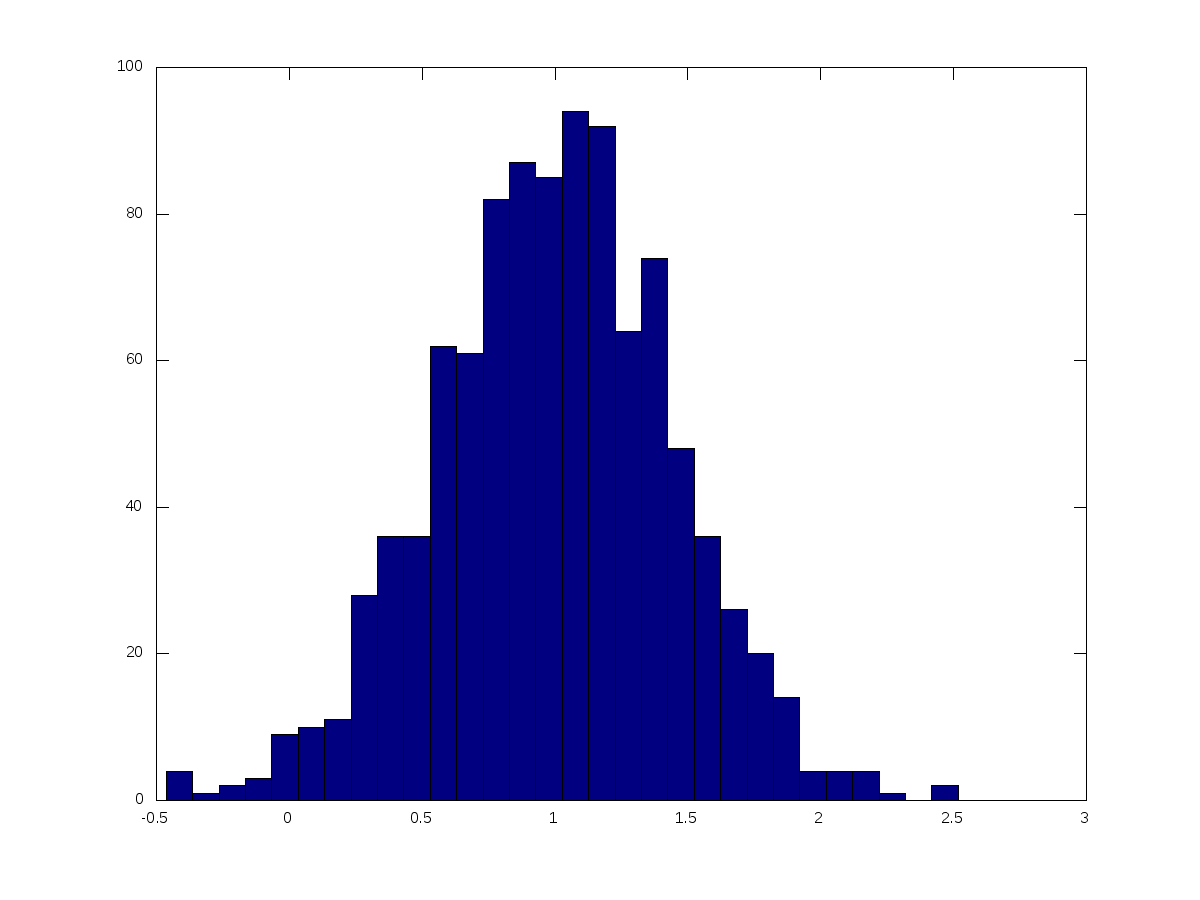
\includegraphics[width=10cm]{Examples/DataProblems/collin_ols}}\subfloat[OLS,$\hat{\beta_{2}}$, dropping x3]{

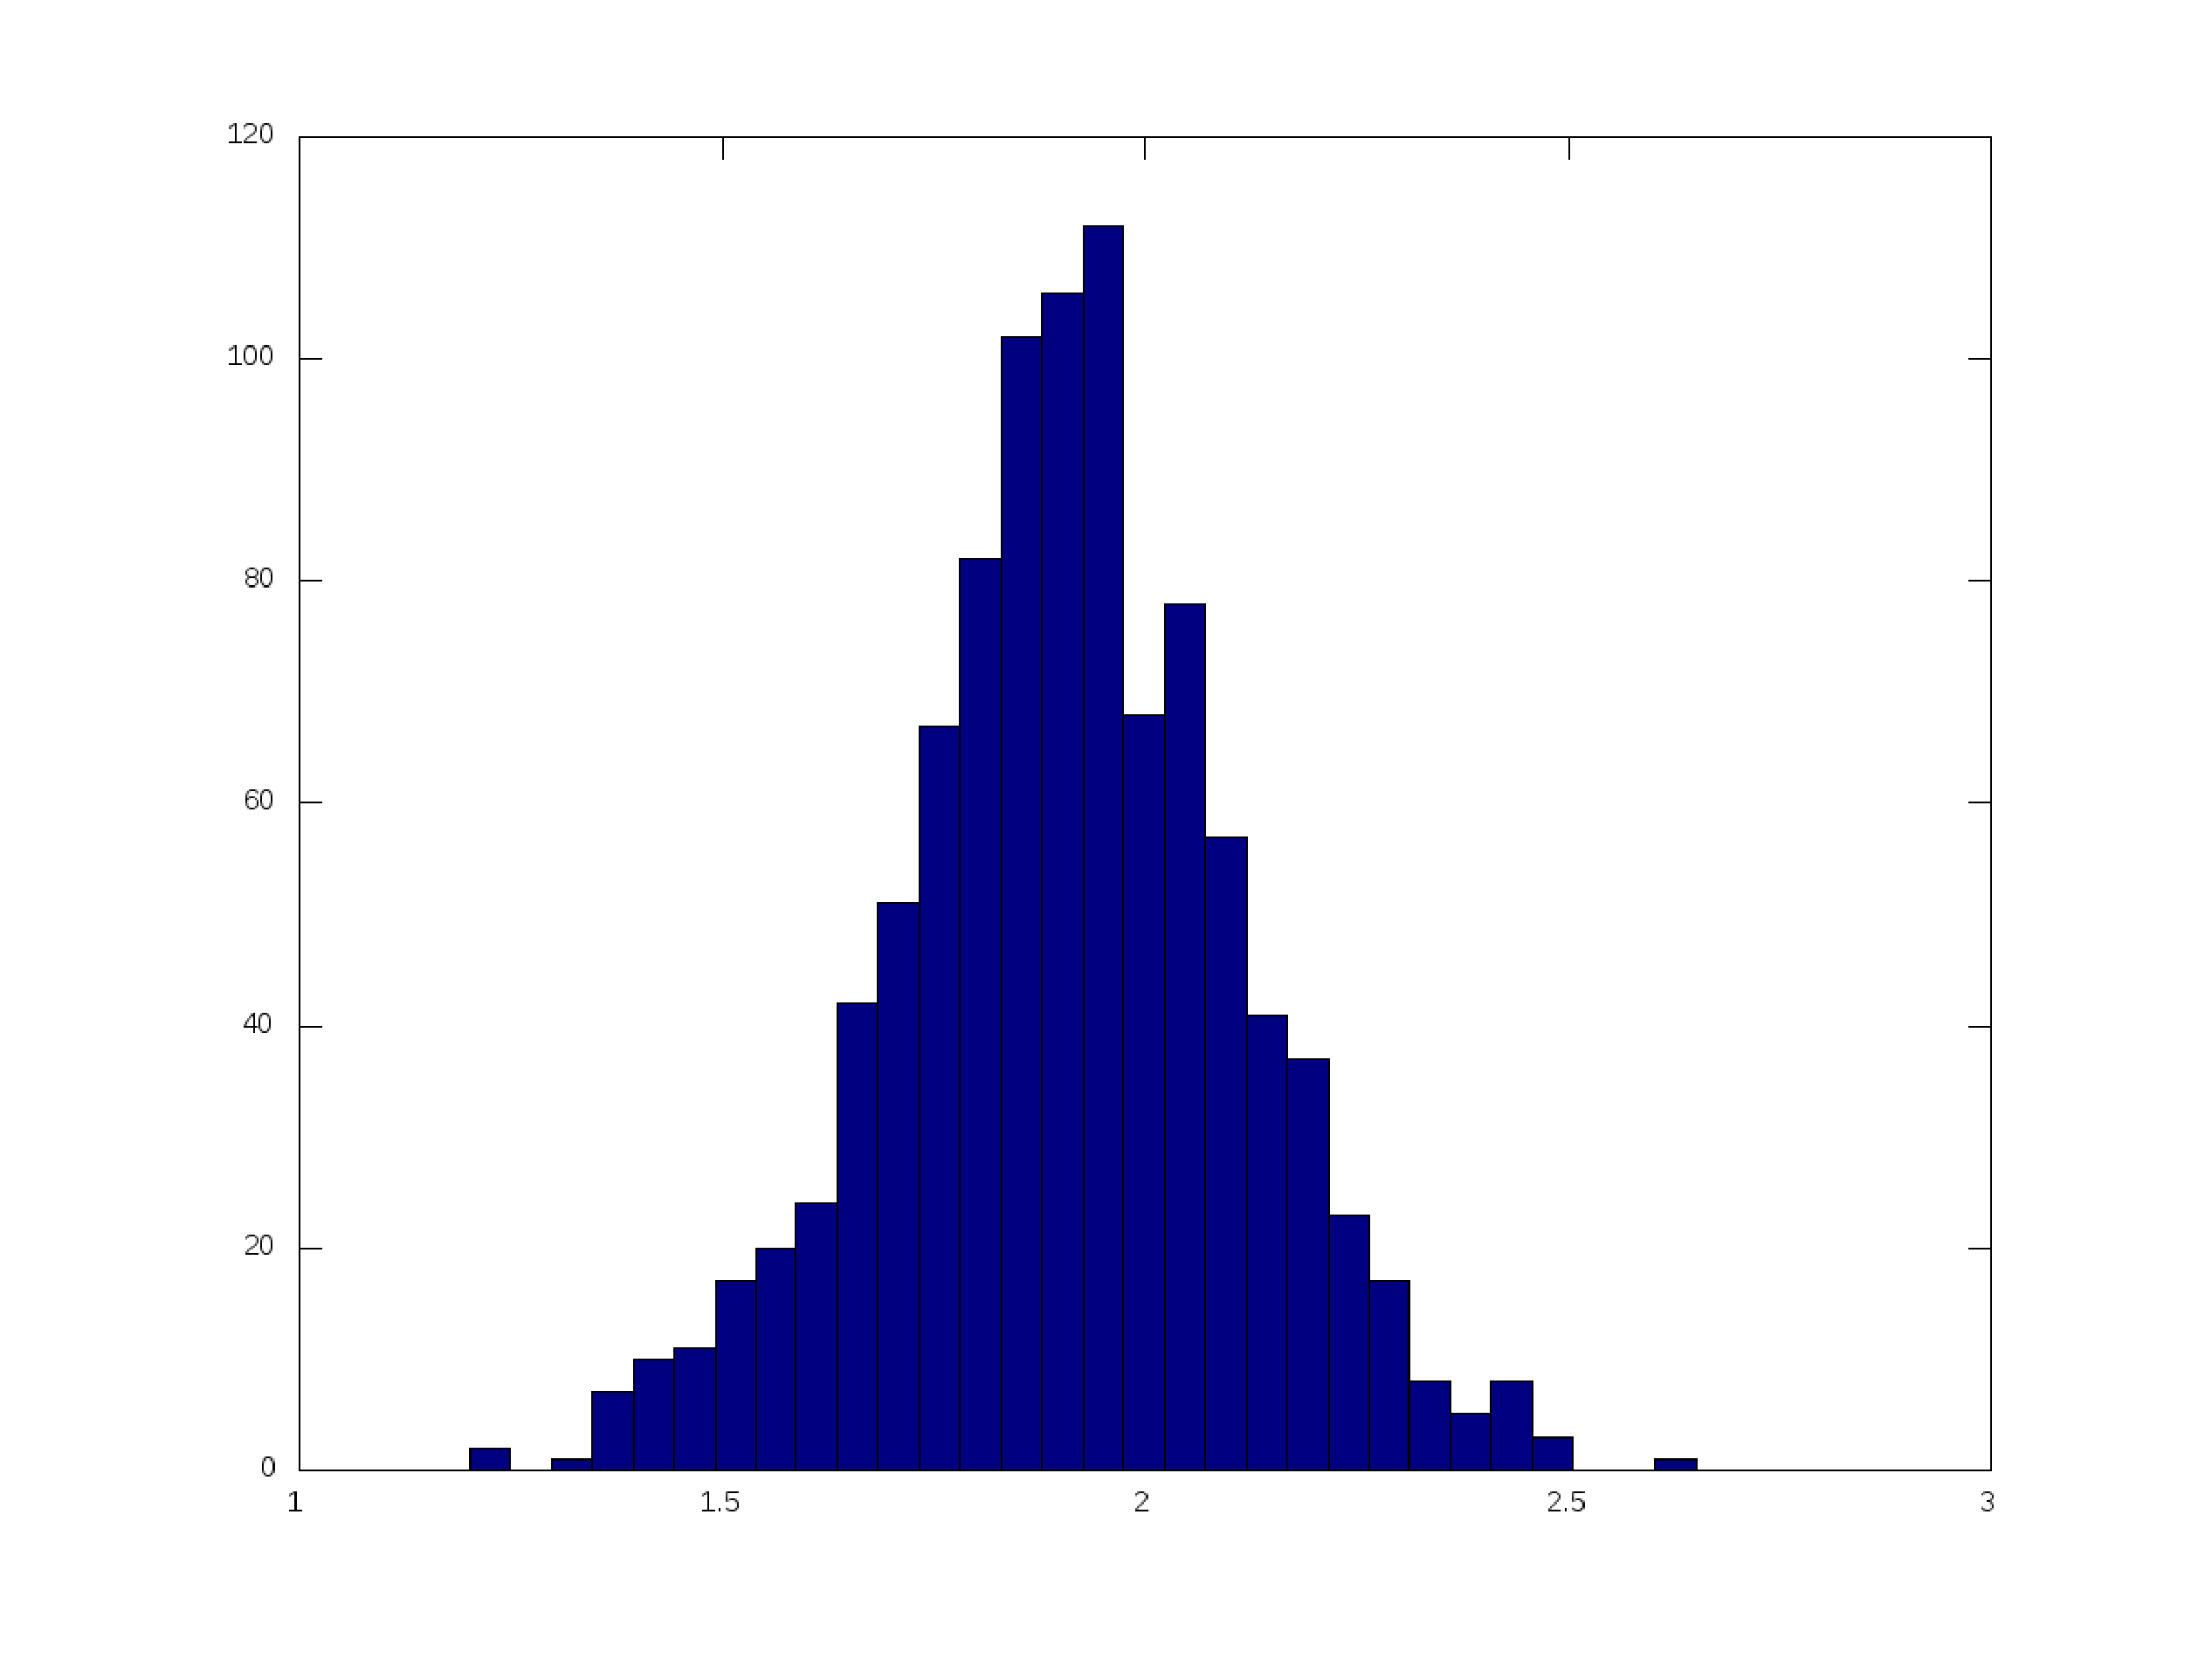
\includegraphics[width=10cm]{Examples/DataProblems/collin_drop}}

\subfloat[Restricted LS,$\hat{\beta_{2}}$, with true restriction$\beta_{2}=\beta_{3}$]{

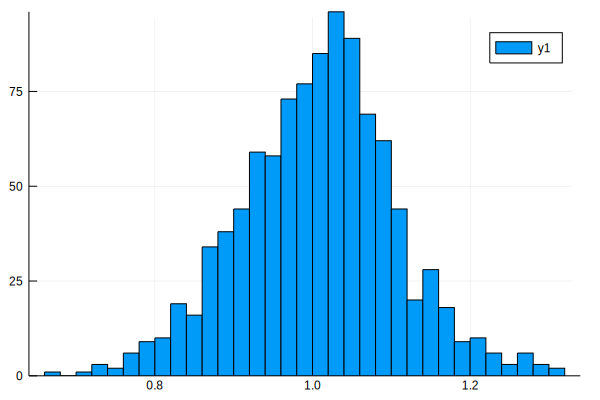
\includegraphics[width=10cm]{Examples/DataProblems/collin_rls}}
\end{figure}



\subsection{Detection of collinearity}

The best way is simply to regress each explanatory variable in turn on the remaining regressors. If any of these auxiliary regressions has a high $R^{2},$ there is a problem of collinearity. Furthermore, this procedure identifies which parameters are affected.
\begin{itemize}
\item Sometimes, we're only interested in certain parameters. Collinearity isn't a problem if it doesn't affect what we're interested in estimating. 
\end{itemize}
An alternative is to examine the matrix of correlations between the regressors. High correlations are sufficient but not necessary for severe collinearity.

Also indicative of collinearity is that the model fits well (high $R^{2}),$ but none of the variables is significantly different from zero (e.g., their separate influences aren't well determined).

In summary, the artificial regressions are the best approach if one wants to be careful.
\begin{example}
Nerlove data and collinearity. The simple Nerlove model is 
\[
\ln C=\beta_{1}+\beta_{2}\ln Q+\beta_{3}\ln P_{L}+\beta_{4}\ln P_{F}+\beta_{5}\ln P_{K}+\epsilon
\]
When this model is estimated by OLS, some coefficients are not significant (see subsection \ref{sub:The-Nerlove-data}). This may be due to collinearity.The Octave script  \htmladdnormallink{DataProblems/NerloveCollinearity.m}{file:///home/michael/Mystuff/Econometrics/Examples/DataProblems/NerloveCollinearity.m}  checks the regressors for collinearity. If you run this, you will see that collinearity is not a problem with this data. Why is the coefficient of $\ln P_{K}$ not significantly different from zero?
\end{example}

\subsection{Dealing with collinearity}


\subsubsection{More information}

Collinearity is a problem of an uninformative sample. The first question is: is all the available information being used? Is more data available? Are there coefficient restrictions that have been neglected? \emph{Picture illustrating how a restriction can solve problem of perfect collinearity.}


\subsubsection{\label{sub:Stochastic-restrictions-and}Stochastic restrictions and ridge regression}

Supposing that there is no more data or neglected restrictions, one possibility is to change perspectives, to Bayesian econometrics. One can express prior beliefs regarding the coefficients using stochastic restrictions. A stochastic linear restriction would be something of the form 
\[
R\beta=r+v
\]
 where $R$ and $r$ are as in the case of exact linear restrictions, but $v$ is a random vector. For example, the model could be 
\begin{eqnarray*}
y & = & X\beta+\varepsilon\\
R\beta & = & r+v\\
\left(\begin{array}{c}
\varepsilon\\
v
\end{array}\right) & \sim & N\left(\begin{array}{c}
0\\
0
\end{array}\right),\left(\begin{array}{cc}
\sigma_{\varepsilon}^{2}I_{n} & 0_{n\times q}\\
0_{q\times n} & \sigma_{v}^{2}I_{q}
\end{array}\right)
\end{eqnarray*}
 This sort of model isn't in line with the classical interpretation of parameters as constants: according to this interpretation the left hand side of $R\beta=r+v$ is constant but the right is random. This model does fit the Bayesian perspective: we combine information coming from the model and the data, summarized in 
\begin{eqnarray*}
y & = & X\beta+\varepsilon\\
\varepsilon & \sim & N(0,\sigma_{\varepsilon}^{2}I_{n})
\end{eqnarray*}
 with prior beliefs regarding the distribution of the parameter, summarized in

\[
R\beta\sim N(r,\sigma_{v}^{2}I_{q})
\]
 Since the sample is random it is reasonable to suppose that $\mathcal{E}(\varepsilon v^{\prime})=0,$ which is the last piece of information in the specification. How can you estimate using this model? The solution is to treat the restrictions as artificial data. Write 
\[
\left[\begin{array}{c}
y\\
r
\end{array}\right]=\left[\begin{array}{c}
X\\
R
\end{array}\right]\beta+\left[\begin{array}{c}
\varepsilon\\
v
\end{array}\right]
\]
 This model is heteroscedastic, since $\sigma_{\varepsilon}^{2}\neq\sigma_{v}^{2}.$ Define the \emph{prior precision} $k=\sigma_{\varepsilon}/\sigma_{v}.$ This expresses the degree of belief in the restriction relative to the variability of the data. Supposing that we specify $k,$ then the model 
\[
\left[\begin{array}{c}
y\\
kr
\end{array}\right]=\left[\begin{array}{c}
X\\
kR
\end{array}\right]\beta+\left[\begin{array}{c}
\varepsilon\\
kv
\end{array}\right]
\]
 is homoscedastic and can be estimated by OLS. Note that this estimator is biased. It is consistent, however, given that $k$ is a fixed constant, even if the restriction is false (this is in contrast to the case of false exact restrictions). To see this, note that there are $Q$ restrictions, where $Q$ is the number of rows of $R.$ As $n\rightarrow\infty,$ these $Q$ artificial observations have no weight in the objective function, so the estimator has the same limiting objective function as the OLS\ estimator, and is therefore consistent.

To motivate the use of stochastic restrictions, consider the expectation of the squared length of $\hat{\beta}$: 
\begin{eqnarray*}
\mathcal{E}(\hat{\beta}^{\prime}\hat{\beta}) & = & \mathcal{E}\left\{ \left(\beta+\left(X^{\prime}X\right)^{-1}X^{\prime}\varepsilon\right)^{\prime}\left(\beta+\left(X^{\prime}X\right)^{-1}X^{\prime}\varepsilon\right)\right\} \\
 & = & \beta^{\prime}\beta+\mathcal{E}\left(\varepsilon^{\prime}X(X^{\prime}X)^{-1}(X^{\prime}X)^{-1}X^{\prime}\varepsilon\right)\\
 & = & \beta^{\prime}\beta+Tr\left(X^{\prime}X\right)^{-1}\sigma^{2}\\
 & = & \beta^{\prime}\beta+\sigma^{2}\sum_{i=1}^{K}\lambda_{i}\text{(the\:\ trace\:\ is\:\ the\:\ sum\:\ of\:\ eigenvalues)}\\
 & > & \beta^{\prime}\beta+\lambda_{\max\left(X^{\prime}X^{-1}\right)}\sigma^{2}\text{(the\:\ eigenvalues\:\ are\:\ all\:\ positive,\:\ since}X^{\prime}X\text{\:\ is\:\ p.d.}
\end{eqnarray*}
 so 
\[
\mathcal{E}(\hat{\beta}^{\prime}\hat{\beta})>\beta^{\prime}\beta+\frac{\sigma^{2}}{\lambda_{\min\left(X^{\prime}X\right)}}
\]
 where $\lambda_{\min\left(X^{\prime}X\right)}$ is the minimum eigenvalue of $X^{\prime}X$ (which is the inverse of the maximum eigenvalue of $(X^{\prime}X)^{-1}).$ As collinearity becomes worse and worse, $X^{\prime}X$ becomes more nearly singular, so $\lambda_{\min\left(X^{\prime}X\right)}$ tends to zero (recall that the determinant is the product of the eigenvalues) and $\mathcal{E}(\hat{\beta}^{\prime}\hat{\beta})$ tends to infinite. On the other hand, $\beta^{\prime}\beta$ is finite.

Now considering the restriction $I_{K}\beta=0+v.$ With this restriction the model becomes 
\[
\left[\begin{array}{c}
y\\
0
\end{array}\right]=\left[\begin{array}{c}
X\\
kI_{K}
\end{array}\right]\beta+\left[\begin{array}{c}
\varepsilon\\
kv
\end{array}\right]
\]
 and the estimator is 
\begin{eqnarray*}
\hat{\beta}_{ridge} & = & \left(\left[\begin{array}{cc}
X^{\prime} & kI_{K}\end{array}\right]\left[\begin{array}{c}
X\\
kI_{K}
\end{array}\right]\right)^{-1}\left[\begin{array}{cc}
X^{\prime} & I_{K}\end{array}\right]\left[\begin{array}{c}
y\\
0
\end{array}\right]\\
 & = & \left(X^{\prime}X+k^{2}I_{K}\right)^{-1}X^{\prime}y
\end{eqnarray*}
 This is the ordinary \emph{ridge regression} estimator. The ridge regression estimator can be seen to add $k^{2}I_{K},$ which is nonsingular, to $X^{\prime}X,$ which is more and more nearly singular as collinearity becomes worse and worse. As $k\rightarrow\infty,$ the restrictions tend to $\beta=0,$ that is, the coefficients are shrunken toward zero. Also, the estimator tends to 
\[
\hat{\beta}_{ridge}=\left(X^{\prime}X+k^{2}I_{K}\right)^{-1}X^{\prime}y\rightarrow\left(k^{2}I_{K}\right)^{-1}X^{\prime}y=\frac{X^{\prime}y}{k^{2}}\rightarrow0
\]
 so $\hat{\beta}_{ridge}^{\prime}\hat{\beta}_{ridge}\rightarrow0.$ This is clearly a false restriction in the limit, if our original model is at all sensible.

There should be some amount of shrinkage that is in fact a true restriction. The problem is to determine the $k$ such that the restriction is correct. The interest in ridge regression centers on the fact that it can be shown that there exists a $k$ such that $MSE(\hat{\beta}_{ridge})<\hat{\beta}_{OLS}.$ The problem is that this $k$ depends on $\beta$ and $\sigma^{2},$ which are unknown.

The ridge trace method plots $\hat{\beta}_{ridge}^{\prime}\hat{\beta}_{ridge}$ as a function of $k,$ and chooses the value of $k$ that ``artistically'' seems appropriate (e.g., where the effect of increasing $k$ dies off). \emph{Draw picture here.} This means of choosing $k$ is obviously subjective. This is not a problem from the Bayesian perspective: the choice of $k$ reflects prior beliefs about the length of $\beta.$

In summary, the ridge estimator offers some hope, but it is impossible to guarantee that it will outperform the OLS estimator. Collinearity is a fact of life in econometrics, and there is no clear solution to the problem.

The Octave script  \htmladdnormallink{DataProblems/RidgeRegression.m}{file:///home/michael/Mystuff/Econometrics/Examples/DataProblems/RidgeRegression.m}  does a Monte Carlo study that shows that ridge regression can help to deal with collinearity. This script generates Figures and, which show the Monte Carlo sampling frequency of the OLS and ridge estimators, after subtracting the true parameter values. You can see that the ridge estimator has much lower RMSE.

\begin{figure}


\caption{OLS and Ridge regression}


\subfloat[OLS]{

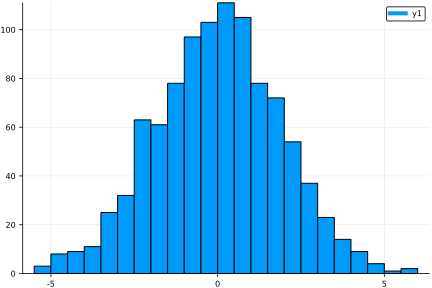
\includegraphics[width=7cm]{Examples/DataProblems/ridge_example_ols}

}\subfloat[Ridge]{

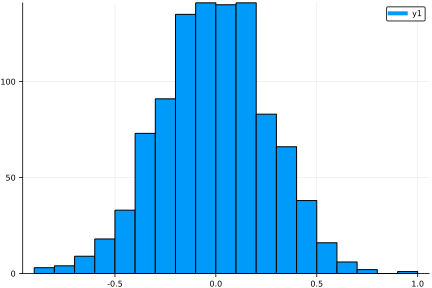
\includegraphics[width=7cm]{Examples/DataProblems/ridge_example_ridge}}

\end{figure}



\section{Measurement error}

Measurement error is exactly what it says, either the dependent variable or the regressors are measured with error. Thinking about the way economic data are reported, measurement error is probably quite prevalent. For example, estimates of growth of GDP, inflation, etc. are commonly revised several times. Why should the last revision necessarily be correct?


\subsection{Error of measurement of the dependent variable}

Measurement errors in the dependent variable and the regressors have important differences. First consider error in measurement of the dependent variable. The data generating process is presumed to be 
\begin{eqnarray*}
y^{*} & = & X\beta+\varepsilon\\
y & = & y^{*}+v\\
v_{t} & \sim & iid(0,\sigma_{v}^{2})
\end{eqnarray*}
where $y^{*}=y+v$ is the unobservable true dependent variable, and $y$ is what is observed. We assume that $\varepsilon$ and $v$ are independent and that $y^{*}=X\beta+\varepsilon$ satisfies the classical assumptions. Given this, we have 
\[
y+v=X\beta+\varepsilon
\]
 so 
\begin{eqnarray*}
y & = & X\beta+\varepsilon-v\\
 & = & X\beta+\omega\\
\omega_{t} & \sim & iid(0,\sigma_{\varepsilon}^{2}+\sigma_{v}^{2})
\end{eqnarray*}

\begin{itemize}
\item As long as $v$ is uncorrelated with $X,$ this model satisfies the classical assumptions and can be estimated by OLS. This type of measurement error isn't a problem, then, except in that the increased variability of the error term causes an increase in the variance of the OLS estimator (see equation \ref{eq:variance factors}). 
\end{itemize}

\subsection{Error of measurement of the regressors}

The situation isn't so good in this case. The DGP is 
\begin{eqnarray*}
y_{t} & = & x_{t}^{*\prime}\beta+\varepsilon_{t}\\
x_{t} & = & x_{t}^{*}+v_{t}\\
v_{t} & \sim & iid(0,\Sigma_{v})
\end{eqnarray*}
where $\Sigma_{v}$ is a $K\times K$ matrix. Now $X^{*}$ contains the true, unobserved regressors, and $X$ is what is observed. Again assume that $v$ is independent of $\varepsilon,$ and that the model $y=X^{*}\beta+\varepsilon$ satisfies the classical assumptions. Now we have 
\begin{eqnarray*}
y_{t} & = & \left(x_{t}-v_{t}\right)^{\prime}\beta+\varepsilon_{t}\\
 & = & x_{t}^{\prime}\beta-v_{t}^{\prime}\beta+\varepsilon_{t}\\
 & = & x_{t}^{\prime}\beta+\omega_{t}
\end{eqnarray*}
 The problem is that now there is a correlation between $x_{t}$ and $\omega_{t},$ since 
\begin{eqnarray*}
\mathcal{E}(x_{t}\omega_{t}) & = & \mathcal{E}\left(\left(x_{t}^{*}+v_{t}\right)\left(-v_{t}^{\prime}\beta+\varepsilon_{t}\right)\right)\\
 & = & -\Sigma_{v}\beta
\end{eqnarray*}
 where 
\[
\Sigma_{v}=\mathcal{E}\left(v_{t}v_{t}^{\prime}\right).
\]
 Because of this correlation, the OLS\ estimator is biased and inconsistent, just as in the case of autocorrelated errors with lagged dependent variables. In matrix notation, write the estimated model as 
\[
y=X\beta+\omega
\]
 We have that 
\[
\hat{\beta}=\left(\frac{X^{\prime}X}{n}\right)^{-1}\left(\frac{X^{\prime}y}{n}\right)
\]
 and 
\begin{eqnarray*}
plim\left(\frac{X^{\prime}X}{n}\right)^{-1} & = & plim\frac{\left(X^{*\prime}+V^{\prime}\right)\left(X^{*}+V\right)}{n}\\
 & = & \left(Q_{X^{*}}+\Sigma_{v}\right)^{-1}
\end{eqnarray*}
 since $X^{*}$ and $V$ are independent, and 
\begin{eqnarray*}
plim\frac{V^{\prime}V}{n} & = & \lim\mathcal{E}\frac{1}{n}\sum_{t=1}^{n}v_{t}v_{t}^{\prime}\\
 & = & \Sigma_{v}
\end{eqnarray*}


Likewise, 
\begin{eqnarray*}
plim\left(\frac{X^{\prime}y}{n}\right) & = & plim\frac{\left(X^{*\prime}+V^{\prime}\right)\left(X^{*}\beta+\varepsilon\right)}{n}\\
 & = & Q_{X^{*}}\beta
\end{eqnarray*}
 so 
\[
plim\hat{\beta}=\left(Q_{X^{*}}+\Sigma_{v}\right)^{-1}Q_{X^{*}}\beta
\]
 So we see that the least squares estimator is inconsistent when the regressors are measured with error.
\begin{itemize}
\item A potential solution to this problem is the instrumental variables (IV) estimator, which we'll discuss shortly. \end{itemize}
\begin{example}
\label{exa:Measurement-error-in}Measurement error in a dynamic model. Consider the model 
\begin{eqnarray*}
y_{t}^{*} & = & \alpha+\rho y_{t-1}^{*}+\beta x_{t}+\epsilon_{t}\\
y_{t} & = & y_{t}^{*}+\upsilon_{t}
\end{eqnarray*}
where $\epsilon_{t}$ and $\upsilon_{t}$ are independent Gaussian white noise errors. Suppose that $y_{t}^{*}$ is not observed, and instead we observe $y_{t}$. What are the properties of the OLS regression on the equation
\[
y_{t}=\alpha+\rho y_{t-1}+\beta x_{t}+\eta_{t}
\]
? The error is 
\begin{align*}
\eta_{t} & =y_{t}-\alpha-\rho y_{t-1}-\beta x_{t}\\
 & =y_{t}^{*}+\upsilon_{t}-\alpha-\rho y_{t-1}^{*}-\rho\upsilon_{t-1}-\beta x_{t}\\
 & =\alpha+\rho y_{t-1}^{*}+\beta x_{t}+\epsilon_{t}+\upsilon_{t}-\alpha-\rho y_{t-1}^{*}-\rho\upsilon_{t-1}-\beta x_{t}\\
 & =\epsilon_{t}+\upsilon_{t}-\rho\upsilon_{t-1}
\end{align*}
So the error term is autocorrelated. Note that 
\[
y_{t-1}=\alpha+\rho y_{t-2}+\beta x_{t-1}+\eta_{t-1}
\]
and 
\[
\eta_{t-1}=\epsilon_{t-1}+\upsilon_{t-1}-\rho\upsilon_{t-2},
\]
so the error $\eta_{t}$ and the regressor $y_{t-1}$ are correlated, because they share the common term $\upsilon_{t-1}.$ This means that the equation 
\[
y_{t}=\alpha+\rho y_{t-1}+\beta x_{t}+\eta_{t}
\]
 does not satisfy weak exogeneity, and the OLS estimator will be biased and inconsistent.

The Octave script  \htmladdnormallink{DataProblems/MeasurementError.m}{file:///home/michael/Mystuff/Econometrics/Examples/DataProblems/MeasurementError.m}  does a Monte Carlo study. The sample size is $n=100$. Figure \ref{fig:measurement error} gives the results. The first panel shows a histogram for 1000 replications of $\hat{\rho}-\rho$, when $\sigma_{\nu}=1$, so that there is significant measurement error. The second panel repeats this with $\sigma_{\nu}=0,$ so that there is not measurement error. Note that there is much more bias with measurement error. There is also bias without measurement error. This is due to the same reason that we saw bias in Figure \ref{figure-biasedness}: one of the classical assumptions (nonstochastic regressors) that guarantees unbiasedness of OLS does not hold for this model. Without measurement error, the OLS estimator \emph{is }consistent. By re-running the script with larger $n$, you can verify that the bias disappears when $\sigma_{\nu}=0$, but not when $\sigma_{\nu}>0$.
\end{example}
\newpage{}
\begin{figure}
\caption{\label{fig:measurement error}$\hat{\rho}-\rho$ with and without measurement error}


\subfloat[with measurement error: $\sigma_{\nu}=1$]{

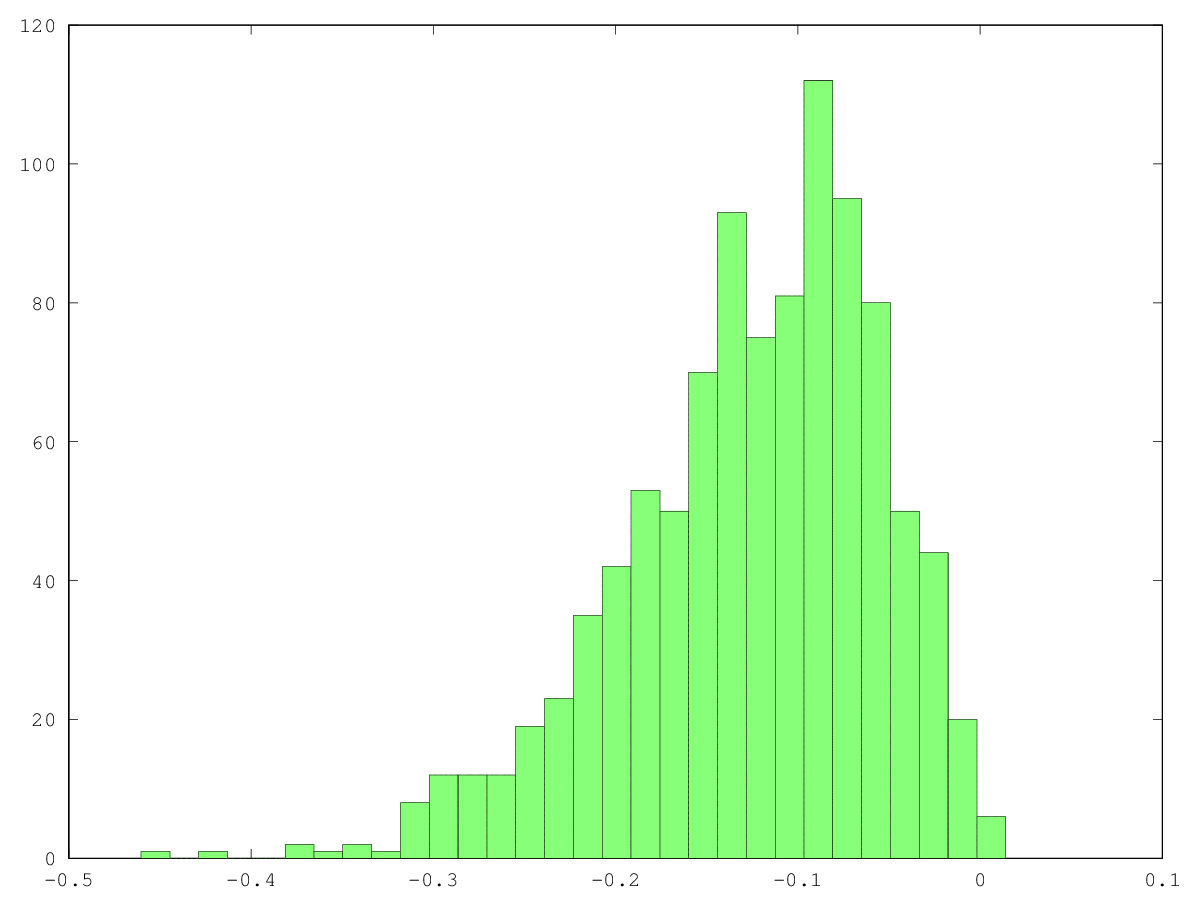
\includegraphics[width=10cm]{Examples/DataProblems/ylag_n100}}\subfloat[without measurement error: $\sigma_{\nu}=0$]{

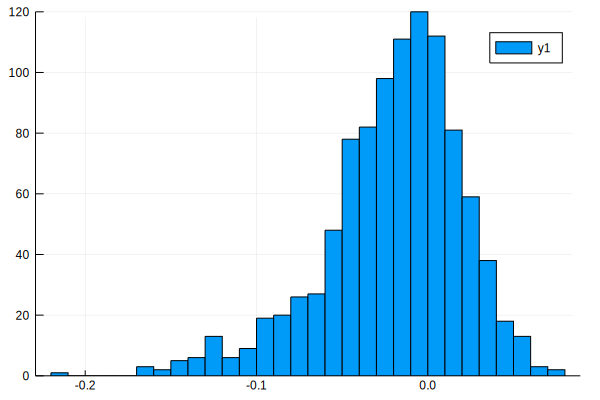
\includegraphics[width=10cm]{Examples/DataProblems/ylag_n100_no_error}}
\end{figure}
\newpage{}


\section{Missing observations}

Missing observations occur quite frequently:\ time series data may not be gathered in a certain year, or respondents to a survey may not answer all questions. We'll consider two cases: missing observations on the dependent variable and missing observations on the regressors.


\subsection{Missing observations on the dependent variable}

In this case, we have 
\[
y=X\beta+\varepsilon
\]
 or 
\[
\left[\begin{array}{c}
y_{1}\\
y_{2}
\end{array}\right]=\left[\begin{array}{c}
X_{1}\\
X_{2}
\end{array}\right]\beta+\left[\begin{array}{c}
\varepsilon_{1}\\
\varepsilon_{2}
\end{array}\right]
\]
 where $y_{2}$ is not observed. Otherwise, we assume the classical assumptions hold.
\begin{itemize}
\item A clear alternative is to simply estimate using the compete observations 
\[
y_{1}=X_{1}\beta+\varepsilon_{1}
\]
 Since these observations satisfy the classical assumptions, one could estimate by OLS.
\item The question remains whether or not one could somehow replace the unobserved $y_{2}$ by a predictor, and improve over OLS in some sense. Let $\hat{y}_{2}$ be the predictor of $y_{2}.$ Now 
\end{itemize}
\begin{eqnarray*}
\hat{\beta} & = & \left\{ \left[\begin{array}{c}
X_{1}\\
X_{2}
\end{array}\right]^{\prime}\left[\begin{array}{c}
X_{1}\\
X_{2}
\end{array}\right]\right\} ^{-1}\left[\begin{array}{c}
X_{1}\\
X_{2}
\end{array}\right]^{\prime}\left[\begin{array}{c}
y_{1}\\
\hat{y}_{2}
\end{array}\right]\\
 & = & \left[X_{1}^{\prime}X_{1}+X_{2}^{\prime}X_{2}\right]^{-1}\left[X_{1}^{\prime}y_{1}+X_{2}^{\prime}\hat{y}_{2}\right]
\end{eqnarray*}
 Recall that the OLS\ fonc are 
\[
X^{\prime}X\hat{\beta}=X^{\prime}y
\]
 so if we regressed using only the first (complete)\ observations, we would have 
\[
X_{1}^{\prime}X_{1}\hat{\beta}_{1}=X_{1}^{\prime}y_{1.}
\]
 Likewise, an OLS regression using only the second (filled in)\ observations would give 
\[
X_{2}^{\prime}X_{2}\hat{\beta}_{2}=X_{2}^{\prime}\hat{y}_{2}.
\]
 Substituting these into the equation for the overall combined estimator gives 
\begin{eqnarray*}
\hat{\beta} & = & \left[X_{1}^{\prime}X_{1}+X_{2}^{\prime}X_{2}\right]^{-1}\left[X_{1}^{\prime}X_{1}\hat{\beta}_{1}+X_{2}^{\prime}X_{2}\hat{\beta}_{2}\right]\\
 & = & \left[X_{1}^{\prime}X_{1}+X_{2}^{\prime}X_{2}\right]^{-1}X_{1}^{\prime}X_{1}\hat{\beta}_{1}+\left[X_{1}^{\prime}X_{1}+X_{2}^{\prime}X_{2}\right]^{-1}X_{2}^{\prime}X_{2}\hat{\beta}_{2}\\
 & \equiv & A\hat{\beta}_{1}+(I_{K}-A)\hat{\beta}_{2}
\end{eqnarray*}
 where 
\[
A\equiv\left[X_{1}^{\prime}X_{1}+X_{2}^{\prime}X_{2}\right]^{-1}X_{1}^{\prime}X_{1}
\]
 and we use 
\begin{eqnarray*}
\left[X_{1}^{\prime}X_{1}+X_{2}^{\prime}X_{2}\right]^{-1}X_{2}^{\prime}X_{2} & = & \left[X_{1}^{\prime}X_{1}+X_{2}^{\prime}X_{2}\right]^{-1}\left[\left(X_{1}^{\prime}X_{1}+X_{2}^{\prime}X_{2}\right)-X_{1}^{\prime}X_{1}\right]\\
 & = & I_{K}-\left[X_{1}^{\prime}X_{1}+X_{2}^{\prime}X_{2}\right]^{-1}X_{1}^{\prime}X_{1}\\
 & = & I_{K}-A.
\end{eqnarray*}


Now, 
\[
\mathcal{E}(\hat{\beta})=A\beta+(I_{K}-A)\mathcal{E}\left(\hat{\beta}_{2}\right)
\]
 and this will be unbiased only if $\mathcal{E}\left(\hat{\beta}_{2}\right)=\beta.$
\begin{itemize}
\item The conclusion is that the filled in observations alone would need to define an unbiased estimator. This will be the case only if 
\[
\hat{y}_{2}=X_{2}\beta+\hat{\varepsilon}_{2}
\]
 where $\hat{\varepsilon}_{2}$ has mean zero. Clearly, it is difficult to satisfy this condition without knowledge of $\beta.$
\item Note that putting $\hat{y}_{2}=\bar{y}_{1}$ does not satisfy the condition and therefore leads to a biased estimator. \end{itemize}
\begin{xca}
Formally prove this last statement.
\end{xca}

\subsection{The sample selection problem}

In the above discussion we assumed that the missing observations are random. The sample selection problem is a case where the missing observations are not random. Consider the model 
\[
y_{t}^{*}=x_{t}^{\prime}\beta+\varepsilon_{t}
\]
 which is assumed to satisfy the classical assumptions. However, $y_{t}^{*\;}$ is not always observed. What is observed is $y_{t}$ defined as 
\[
y_{t}=y_{t}^{*}\text{\textnormal{ }if }y_{t}^{*}\geq0
\]
 Or, in other words, $y_{t}^{*}$ is missing when it is less than zero.

The difference in this case is that the missing values are not random:\ they are correlated with the $x_{t}.$ Consider the case 
\[
y^{*}=x+\varepsilon
\]
 with $V(\varepsilon)=25$, but using only the observations for which $y^{*}>0$ to estimate. Figure \ref{cap:Sample-selection-bias} illustrates the bias. The Octave program is  \htmladdnormallink{sampsel.m}{file:///home/michael/Mystuff/Econometrics/Examples/Figures/sampsel.m} 

\begin{figure}
\caption{\label{cap:Sample-selection-bias}Sample selection bias}


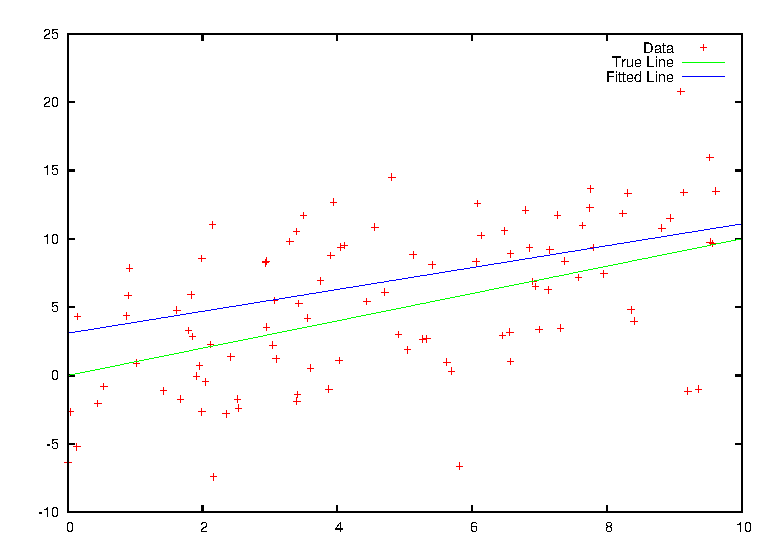
\includegraphics{Examples/Figures/sampsel}
\end{figure}
There are means of dealing with sample selection bias, but we will not go into it here. One should at least be aware that nonrandom selection of the sample will normally lead to bias and inconsistency if the problem is not taken into account.


\subsection{Missing observations on the regressors}

Again the model is 
\[
\left[\begin{array}{c}
y_{1}\\
y_{2}
\end{array}\right]=\left[\begin{array}{c}
X_{1}\\
X_{2}
\end{array}\right]\beta+\left[\begin{array}{c}
\varepsilon_{1}\\
\varepsilon_{2}
\end{array}\right]
\]
 but we assume now that each row of $X_{2}$ has an unobserved component(s). Again, one could just estimate using the complete observations, but it may seem frustrating to have to drop observations simply because of a single missing variable. In general, if the unobserved $X_{2}$ is replaced by some prediction, $X_{2}^{*},$ then we are in the case of errors of observation. As before, this means that the OLS\ estimator is biased when $X_{2}^{*}$ is used instead of $X_{2}.$ Consistency is salvaged, however, as long as the number of missing observations doesn't increase with $n.$
\begin{itemize}
\item Including observations that have missing values replaced by \emph{ad hoc} values can be interpreted as introducing false stochastic restrictions. In general, this introduces bias. It is difficult to determine whether MSE increases or decreases. Monte Carlo studies suggest that it is dangerous to simply substitute the mean, for example.
\item In the case that there is only one regressor other than the constant, subtitution of $\bar{x}$ for the missing $x_{t}$ \emph{does not lead to bias}. This is a special case that doesn't hold for $K>2.$\end{itemize}
\begin{xca}
Prove this last statement.\end{xca}
\begin{itemize}
\item In summary, if one is strongly concerned with bias, it is best to drop observations that have missing components. There is potential for reduction of MSE through filling in missing elements with intelligent guesses, but this could also increase MSE. 
\end{itemize}

\section{\label{sec:Missing-regressors}Missing regressors}

Suppose that the model $y=X\beta+W\gamma+\epsilon$ satisfies the classical assumptions, so OLS would be a consistent estimator. However, let's suppose that the regressors $W$ are not available in the sample. What are the properties of the OLS estimator of the model $y=X\beta+\omega?$ We can think of this as a case of imposing false restrictions: $\gamma=0$ when in fact $\gamma\ne0$. We know that the restricted least squares estimator is biased and inconsistent, in general, when we impose false restrictions. Another way of thinking of this is to look to see if $X$ and $\omega$ are correlated. We have
\begin{align*}
E(X_{t}\omega_{t}) & =E\left(X_{t}\left(W_{t}^{\prime}\gamma+\epsilon_{t}\right)\right)\\
 & =E(X_{t}W_{t}^{\prime}\gamma)+E(X_{t}\epsilon_{t})\\
 & =E(X_{t}W_{t}^{\prime}\gamma)
\end{align*}
where the last line follows because $E(X_{t}\epsilon_{t})=0$ by assumption. So, there will be correlation between the error and the regressors if there is collinearity between the included regressors $X_{t}$ and the missing regressors $W_{t}$. If there is not, the OLS estimator will be consistent. Because the normal thing is to have collinearity between regressors, we expect that missing regressors will lead to bias and inconsistency of the OLS estimator.


\section{Exercises}
\begin{enumerate}
\item Consider the simple Nerlove model 
\[
\ln C=\beta_{1}+\beta_{2}\ln Q+\beta_{3}\ln P_{L}+\beta_{4}\ln P_{F}+\beta_{5}\ln P_{K}+\epsilon
\]
When this model is estimated by OLS, some coefficients are not significant. We have seen that collinearity is not an important problem. Why is $\beta_{5}$ not significantly different from zero? Give an economic explanation.
\item For the model $y=\beta_{1}x_{1}+\beta_{2}x_{2}+\epsilon,$

\begin{enumerate}
\item verify that the level sets of the OLS criterion function (defined in equation \ref{eq:OLS criterion function}) are straight lines when there is perfect collinearity
\item For this model with perfect collinearity, the OLS estimator does not exist. Depict what this statement means using a drawing.
\item Show how a restriction $R_{1}\beta_{1}+R_{2}\beta_{2}=r$ causes the restricted least squares estimator to exist, using a drawing.
\end{enumerate}
\end{enumerate}
\newpage{}


\chapter{Functional form and nonnested tests}

Though theory often suggests which conditioning variables should be included, and suggests the signs of certain derivatives, it is usually silent regarding the functional form of the relationship between the dependent variable and the regressors. For example, considering a cost function, one could have a Cobb-Douglas model 
\[
c=Aw_{1}^{\beta_{1}}w_{2}^{\beta_{2}}q^{\beta_{q}}e^{\varepsilon}
\]
 This model, after taking logarithms, gives 
\[
\ln c=\beta_{0}+\beta_{1}\ln w_{1}+\beta_{2}\ln w_{2}+\beta_{q}\ln q+\varepsilon
\]
 where $\beta_{0}=\ln A.$ Theory suggests that $A>0,\beta_{1}>0,\beta_{2}>0,\beta_{3}>0.$ This model isn't compatible with a fixed cost of production since $c=0$ when $q=0.$ Homogeneity of degree one in input prices suggests that $\beta_{1}+\beta_{2}=1,$ while constant returns to scale implies $\beta_{q}=1.$

While this model may be reasonable in some cases, an alternative 
\[
\sqrt{c}=\beta_{0}+\beta_{1}\sqrt{w_{1}}+\beta_{2}\sqrt{w_{2}}+\beta_{q}\sqrt{q}+\varepsilon
\]
 may be just as plausible. Note that $\sqrt{x}$ and $\ln(x)$ look quite alike, for certain values of the regressors, and up to a linear transformation, so it may be difficult to choose between these models.

The basic point is that many functional forms are compatible with the linear-in-parameters model, since this model can incorporate a wide variety of nonlinear transformations of the dependent variable and the regressors. For example, suppose that $g(\cdot)$ is a real valued function and that $x(\cdot)$ is a $K-$ vector-valued function. The following model is linear in the parameters but nonlinear in the variables: 
\begin{eqnarray*}
x_{t} & = & x(z_{t})\\
y_{t} & = & x_{t}^{\prime}\beta+\varepsilon_{t}
\end{eqnarray*}
 There may be $P$ fundamental conditioning variables $z_{t}$, but there may be $K$ regressors, where $K$ may be smaller than, equal to or larger than $P.$ For example, $x_{t}$ could include squares and cross products of the conditioning variables in $z_{t}.$


\section{Flexible functional forms}

Given that the functional form of the relationship between the dependent variable and the regressors is in general unknown, one might wonder if there exist parametric models that can closely approximate a wide variety of functional relationships. A ``Diewert-Flexible'' functional form is defined as one such that the function, the vector of first derivatives and the matrix of second derivatives can take on an arbitrary value \emph{at a single data point.} Flexibility in this sense clearly requires that there be at least 
\[
K=1+P+\left(P^{2}-P\right)/2+P
\]
 free parameters: one for each independent effect that we wish to model.

Suppose that the model is 
\[
y=g(x)+\varepsilon
\]
 A second-order Taylor's series expansion (with remainder term) of the function $g(x)$ about the point $x=0$ is 
\[
g(x)=g(0)+x^{\prime}D_{x}g(0)+\frac{x^{\prime}D_{x}^{2}g(0)x}{2}+R
\]
 Use the approximation, which simply drops the remainder term, as an approximation to $g(x):$
\[
g(x)\simeq g_{K}(x)=g(0)+x^{\prime}D_{x}g(0)+\frac{x^{\prime}D_{x}^{2}g(0)x}{2}
\]
 As $x\rightarrow0,$ the approximation becomes more and more exact, in the sense that $g_{K}(x)\rightarrow g(x),$ $D_{x}g_{K}(x)\rightarrow D_{x}g(x)$ and $D_{x}^{2}g_{K}(x)\rightarrow D_{x}^{2}g(x).$ For $x=0,$ the approximation is exact, up to the second order. The idea behind many flexible functional forms is to note that $g(0),$ $D_{x}g(0)$ and $D_{x}^{2}g(0)$ are all constants. If we treat them as parameters, the approximation will have exactly enough free parameters to approximate the function $g(x),$ which is of unknown form, exactly, up to second order, at the point $x=0.$ The model is 
\[
g_{K}(x)=\alpha+x^{\prime}\beta+1/2x^{\prime}\Gamma x
\]
 so the regression model to fit is 
\[
y=\alpha+x^{\prime}\beta+1/2x^{\prime}\Gamma x+\varepsilon
\]

\begin{itemize}
\item While the regression model has enough free parameters to be Diewert-flexible, the question remains: is $plim\hat{\alpha}=g(0)?$ Is $plim\hat{\beta}=D_{x}g(0)?$ Is $plim\hat{\Gamma}=D_{x}^{2}g(0)?$
\item The answer is no, in general. The reason is that if we treat the true values of the parameters as these derivatives, then $\varepsilon$ is forced to play the part of the remainder term, which is a function of $x,$ so that $x$ and $\varepsilon$ are correlated in this case. As before, the estimator is biased in this case.
\item A simpler example would be to consider a first-order T.S. approximation to a quadratic function. \emph{Draw picture.}
\item The conclusion is that ``flexible functional forms'' aren't really flexible in a useful statistical sense, in that neither the function itself nor its derivatives are consistently estimated, unless the function belongs to the parametric family of the specified functional form. In order to lead to consistent inferences, the regression model must be correctly specified. 
\end{itemize}

\subsection{The translog form}

In spite of the fact that FFF's aren't really flexible for the purposes of econometric estimation and inference, they are useful, and they are certainly subject to less bias due to misspecification of the functional form than are many popular forms, such as the Cobb-Douglas or the simple linear in the variables model. The translog model is probably the most widely used FFF. This model is as above, except that the variables are subjected to a logarithmic tranformation. Also, the expansion point is usually taken to be the sample mean of the data, after the logarithmic transformation. The model is defined by 
\begin{eqnarray*}
y & = & \ln(c)\\
x & = & \ln\left(\frac{z}{\bar{z}}\right)\\
 & = & \ln(z)-\ln(\bar{z})\\
y & = & \alpha+x^{\prime}\beta+1/2x^{\prime}\Gamma x+\varepsilon
\end{eqnarray*}
 In this presentation, the $t$ subscript that distinguishes observations is suppressed for simplicity. Note that 
\begin{eqnarray*}
\frac{\partial y}{\partial x} & = & \beta+\Gamma x\\
 & = & \frac{\partial\ln(c)}{\partial\ln(z)}\text{\:(the\:\ other\:\ part\:\ of\:}x\,\text{is\:\ constant)}\\
 & = & \frac{\partial c}{\partial z}\frac{z}{c}
\end{eqnarray*}
 which is the elasticity of $c$ with respect to $z.$ This is a convenient feature of the translog model. Note that at the means of the conditioning variables, $\bar{z}$, $x=0,$ so 
\[
\left.\frac{\partial y}{\partial x}\right|_{z=\bar{z}}=\beta
\]
 so the $\beta$ are the first-order elasticities, at the means of the data.

To illustrate, consider that $y$ is cost of production: 
\[
y=c(w,q)
\]
 where $w$ is a vector of input prices and $q$ is output. We could add other variables by extending $q$ in the obvious manner, but this is supressed for simplicity. By Shephard's lemma, the conditional factor demands are 
\[
x=\frac{\partial c(w,q)}{\partial w}
\]
 and the cost shares of the factors are therefore 
\[
s=\frac{wx}{c}=\frac{\partial c(w,q)}{\partial w}\frac{w}{c}
\]
 which is simply the vector of elasticities of cost with respect to input prices. If the cost function is modeled using a translog function, we have 
\begin{eqnarray*}
\ln(c) & = & \alpha+x^{\prime}\beta+z^{\prime}\delta+1/2\left[\begin{array}{cc}
x^{\prime} & z\end{array}\right]\left[\begin{array}{cc}
\Gamma_{11} & \Gamma_{12}\\
\Gamma_{12}^{\prime} & \Gamma_{22}
\end{array}\right]\left[\begin{array}{c}
x\\
z
\end{array}\right]\\
 & = & \alpha+x^{\prime}\beta+z^{\prime}\delta+1/2x^{\prime}\Gamma_{11}x+x^{\prime}\Gamma_{12}z+1/2z^{2}\gamma_{22}
\end{eqnarray*}
 where $x=\ln(w/\bar{w})$ (element-by-element division) and $z=\ln(q/\bar{q}),$ and 
\begin{eqnarray*}
\Gamma_{11} & = & \left[\begin{array}{ll}
\gamma_{11} & \gamma_{12}\\
\gamma_{12} & \gamma_{22}
\end{array}\right]\\
\Gamma_{12} & = & \left[\begin{array}{l}
\gamma_{13}\\
\gamma_{23}
\end{array}\right]\\
\Gamma_{22} & = & \gamma_{33}.
\end{eqnarray*}
 Note that symmetry of the second derivatives has been imposed.

Then the share equations are just 
\[
s=\beta+\left[\begin{array}{cc}
\Gamma_{11} & \Gamma_{12}\end{array}\right]\left[\begin{array}{c}
x\\
z
\end{array}\right]
\]
 Therefore, the share equations and the cost equation have parameters in common. By pooling the equations together and imposing the (true) restriction that the parameters of the equations be the same, we can gain efficiency.

To illustrate in more detail, consider the case of two inputs, so 
\[
x=\left[\begin{array}{l}
x_{1}\\
x_{2}
\end{array}\right].
\]
 In this case the translog model of the logarithmic cost function is 
\[
\ln c=\alpha+\beta_{1}x_{1}+\beta_{2}x_{2}+\delta z+\frac{\gamma_{11}}{2}x_{1}^{2}+\frac{\gamma_{22}}{2}x_{2}^{2}+\frac{\gamma_{33}}{2}z^{2}+\gamma_{12}x_{1}x_{2}+\gamma_{13}x_{1}z+\gamma_{23}x_{2}z
\]
 The two cost shares of the inputs are the derivatives of $\ln c$ with respect to $x_{1}$ and $x_{2}$: 
\begin{eqnarray*}
s_{1} & = & \beta_{1}+\gamma_{11}x_{1}+\gamma_{12}x_{2}+\gamma_{13}z\\
s_{2} & = & \beta_{2}+\gamma_{12}x_{1}+\gamma_{22}x_{2}+\gamma_{13}z
\end{eqnarray*}


Note that the share equations and the cost equation have parameters in common. One can do a pooled estimation of the three equations at once, imposing that the parameters are the same. In this way we're using more observations and therefore more information, which will lead to imporved efficiency. Note that this does assume that the cost equation is correctly specified (\emph{i.e.,} not an approximation), since otherwise the derivatives would not be the true derivatives of the log cost function, and would then be misspecified for the shares. To pool the equations, write the model in matrix form (adding in error terms) 
\[
\left[\begin{array}{l}
\ln c\\
s_{1}\\
s_{2}
\end{array}\right]=\left[\begin{array}{llllllllll}
1 & x_{1} & x_{2} & z & \frac{x_{1}^{2}}{2} & \frac{x_{2}^{2}}{2} & \frac{z^{2}}{2} & x_{1}x_{2} & x_{1}z & x_{2}z\\
0 & 1 & 0 & 0 & x_{1} & 0 & 0 & x_{2} & z & 0\\
0 & 0 & 1 & 0 & 0 & x_{2} & 0 & x_{1} & 0 & z
\end{array}\right]\left[\begin{array}{l}
\alpha\\
\beta_{1}\\
\beta_{2}\\
\delta\\
\gamma_{11}\\
\gamma_{22}\\
\gamma_{33}\\
\gamma_{12}\\
\gamma_{13}\\
\gamma_{23}
\end{array}\right]+\left[\begin{array}{l}
\varepsilon_{1}\\
\varepsilon_{2}\\
\varepsilon_{3}
\end{array}\right]
\]


This is \emph{one} observation on the three equations. With the appropriate notation, a single observation can be written as 
\[
y_{t}={X_{t}\theta}+\varepsilon_{t}
\]
 The overall model would stack $n$ observations on the three equations for a total of $3n$ observations: 
\[
\left[\begin{array}{l}
y_{1}\\
y_{2}\\
\vdots\\
y_{n}
\end{array}\right]=\left[\begin{array}{l}
X_{1}\\
X_{2}\\
\vdots\\
X_{n}
\end{array}\right]\theta+\left[\begin{array}{l}
\varepsilon_{1}\\
\varepsilon_{2}\\
\vdots\\
\varepsilon_{n}
\end{array}\right]
\]
 Next we need to consider the errors. For observation $t$ the errors can be placed in a vector 
\[
\varepsilon_{t}=\left[\begin{array}{l}
\varepsilon_{1t}\\
\varepsilon_{2t}\\
\varepsilon_{3t}
\end{array}\right]
\]


First consider the covariance matrix of this vector:\ the shares are certainly correlated since they must sum to one. (In fact, with 2 shares the variances are equal and the covariance is -1 times the variance. General notation is used to allow easy extension to the case of more than 2 inputs). Also, it's likely that the shares and the cost equation have different variances. Supposing that the model is covariance stationary, the variance of $\varepsilon_{t}$ won$^{\prime}$t depend upon $t$: 
\[
Var\varepsilon_{t}=\Sigma_{0}=\left[\begin{array}{lll}
\sigma_{11} & \sigma_{12} & \sigma_{13}\\
\cdot & \sigma_{22} & \sigma_{23}\\
\cdot & \cdot & \sigma_{33}
\end{array}\right]
\]
 Note that this matrix is singular, since the shares sum to 1. Assuming that there is no autocorrelation, the overall covariance matrix has the \emph{seemingly unrelated regressions} (SUR) structure. 
\begin{eqnarray*}
Var\left[\begin{array}{l}
\varepsilon_{1}\\
\varepsilon_{2}\\
\vdots\\
\varepsilon_{n}
\end{array}\right] & = & \Sigma\\
 & = & \left[\begin{array}{llll}
\Sigma_{0} & 0 & \cdots & 0\\
0 & \Sigma_{0} & \ddots & \vdots\\
\vdots & \ddots &  & 0\\
0 & \cdots & 0 & \Sigma_{0}
\end{array}\right]\\
 & = & I_{n}\otimes\Sigma_{0}
\end{eqnarray*}
 where the symbol $\otimes$ indicates the \emph{Kronecker product}. The Kronecker product of two matrices $A$ and $B$ is 
\[
A\otimes B=\left[\begin{array}{llll}
a_{11}B & a_{12}B & \cdots & a_{1q}B\\
a_{21}B & \ddots &  & \vdots\\
\vdots\\
a_{pq}B & \cdots &  & a_{pq}B
\end{array}\right].
\]
 


\subsection{FGLS estimation of a translog model}

So, this model has heteroscedasticity and autocorrelation, so OLS\ won't be efficient. The next question is: how do we estimate efficiently using FGLS? FGLS is based upon inverting the estimated error covariance $\hat{\Sigma}.$ So we need to estimate $\Sigma.$

An asymptotically efficient procedure is (supposing normality of the errors)
\begin{enumerate}
\item Estimate each equation by OLS
\item Estimate $\Sigma_{0}$ using 
\[
\hat{\Sigma}_{0}=\frac{1}{n}\sum_{t=1}^{n}\hat{\varepsilon}_{t}\hat{\varepsilon}_{t}^{\prime}
\]

\item Next we need to account for the singularity of $\Sigma_{0}.$ It can be shown that $\hat{\Sigma}_{0}$ will be singular when the shares sum to one, so FGLS won't work. The solution is to drop one of the share equations, for example the second. The model becomes 
\[
\left[\begin{array}{l}
\ln c\\
s_{1}
\end{array}\right]=\left[\begin{array}{llllllllll}
1 & x_{1} & x_{2} & z & \frac{x_{1}^{2}}{2} & \frac{x_{2}^{2}}{2} & \frac{z^{2}}{2} & x_{1}x_{2} & x_{1}z & x_{2}z\\
0 & 1 & 0 & 0 & x_{1} & 0 & 0 & x_{2} & z & 0
\end{array}\right]\left[\begin{array}{l}
\alpha\\
\beta_{1}\\
\beta_{2}\\
\delta\\
\gamma_{11}\\
\gamma_{22}\\
\gamma_{33}\\
\gamma_{12}\\
\gamma_{13}\\
\gamma_{23}
\end{array}\right]+\left[\begin{array}{l}
\varepsilon_{1}\\
\varepsilon_{2}
\end{array}\right]
\]
 or in matrix notation for the observation: 
\[
y_{t}^{\ast}=X_{t}^{\ast}\theta+\varepsilon_{t}^{\ast}
\]
 and in stacked notation for all observations we have the $2n$ observations: 
\[
\left[\begin{array}{l}
y_{1}^{\ast}\\
y_{2}^{\ast}\\
\vdots\\
y_{n}^{\ast}
\end{array}\right]=\left[\begin{array}{l}
X_{1}^{\ast}\\
X_{2}^{\ast}\\
\vdots\\
X_{n}^{\ast}
\end{array}\right]\theta+\left[\begin{array}{l}
\varepsilon_{1}^{\ast}\\
\varepsilon_{2}^{\ast}\\
\vdots\\
\varepsilon_{n}^{\ast}
\end{array}\right]
\]
 or, finally in matrix notation for all observations: 
\[
y^{\ast}=X^{\ast}\theta+\varepsilon^{\ast}
\]
 Considering the error covariance, we can define 
\begin{eqnarray*}
\Sigma_{0}^{\ast} & = & Var\left[\begin{array}{l}
\varepsilon_{1}\\
\varepsilon_{2}
\end{array}\right]\\
\Sigma^{\ast} & = & I_{n}\otimes\Sigma_{0}^{\ast}
\end{eqnarray*}
 Define $\hat{\Sigma}_{0}^{\ast}$ as the leading $2\times2$ block of $\hat{\Sigma}_{0}$ , and form 
\[
\hat{\Sigma}^{\ast}=I_{n}\otimes\hat{\Sigma}_{0}^{\ast}.
\]
 This is a consistent estimator, following the consistency of OLS\ and applying a LLN.
\item Next compute the Cholesky factorization 
\[
\hat{P}_{0}=Chol\left(\hat{\Sigma}_{0}^{\ast}\right)^{-1}
\]
 (I am assuming this is defined as an upper triangular matrix, which is consistent with the way Octave does it) and the Cholesky factorization of the overall covariance matrix of the 2 equation model, which can be calculated as 
\[
\hat{P}=Chol\hat{\Sigma}^{\ast}=I_{n}\otimes\hat{P}_{0}
\]

\item Finally the FGLS\ estimator can be calculated by applying OLS\ to the transformed model 
\[
\hat{P}^{\prime}y^{\ast}=\hat{P}^{\prime}X^{\ast}\theta+\hat{\hat{P}^{\prime}}\varepsilon^{\ast}
\]
 or by directly using the GLS\ formula 
\[
\hat{\theta}_{FGLS}=\left(X^{\ast\prime}\left(\hat{\Sigma}_{0}^{\ast}\right)^{-1}X^{\ast}\right)^{-1}X^{\ast\prime}\left(\hat{\Sigma}_{0}^{\ast}\right)^{-1}y^{\ast}
\]



It is equivalent to transform each observation individually: 
\[
\hat{P}_{0}^{\prime}y_{y}^{\ast}=\hat{P}_{0}^{\prime}X_{t}^{\ast}\theta+\hat{P}_{0}^{\prime}\varepsilon^{\ast}
\]
 and then apply OLS. This is probably the simplest approach.

\end{enumerate}
A few last comments.
\begin{enumerate}
\item We have assumed no autocorrelation across time. This is clearly restrictive. It is relatively simple to relax this, but we won't go into it here.
\item Also, we have only imposed symmetry of the second derivatives. Another restriction that the model should satisfy is that the estimated shares should sum to 1. This can be accomplished by imposing 
\begin{eqnarray*}
\beta_{1}+\beta_{2} & = & 1\\
\sum_{i=1}^{3}\gamma_{ij} & = & 0,\textnormal{ }j=1,2,3.
\end{eqnarray*}
 These are linear parameter restrictions, so they are easy to impose and will improve efficiency if they are true.
\item The estimation procedure outlined above can be \emph{iterated.} That is, estimate $\hat{\theta}_{FGLS}$ as above, then re-estimate $\Sigma_{0}^{\ast}$ using errors calculated as 
\[
\hat{\varepsilon}=y-X\hat{\theta}_{FGLS}
\]



These might be expected to lead to a better estimate than the estimator based on $\hat{\theta}_{OLS},$ since FGLS\ is asymptotically more efficient. Then re-estimate $\theta$ using the new estimated error covariance. It can be shown that if this is repeated until the estimates don't change (\emph{i.e.,} iterated to convergence) then the resulting estimator is the MLE. At any rate, the asymptotic properties of the iterated and uniterated estimators are the same, since both are based upon a consistent estimator of the error covariance. 

\end{enumerate}

\section{Testing nonnested hypotheses}

Given that the choice of functional form isn't perfectly clear, in that many possibilities exist, how can one choose between forms? When one form is a parametric restriction of another, the previously studied tests such as Wald, LR, score or $qF$ are all possibilities. For example, the Cobb-Douglas model is a parametric restriction of the translog: The translog is 
\[
y_{t}=\alpha+x_{t}^{\prime}\beta+1/2x_{t}^{\prime}\Gamma x_{t}+\varepsilon
\]
 where the variables are in logarithms, while the Cobb-Douglas is 
\[
y_{t}=\alpha+x_{t}^{\prime}\beta+\varepsilon
\]
 so a test of the Cobb-Douglas versus the translog is simply a test that $\Gamma=0.$

The situation is more complicated when we want to test \emph{non-nested hypotheses.} If the two functional forms are linear in the parameters, and use the same transformation of the dependent variable, then they may be written as 
\begin{eqnarray*}
M_{1}:y & = & X\beta+\varepsilon\\
\varepsilon_{t} & \sim & iid(0,\sigma_{\varepsilon}^{2})\\
M_{2}:y & = & Z\gamma+\eta\\
\eta & \sim & iid(0,\sigma_{\eta}^{2})
\end{eqnarray*}
 We wish to test hypotheses of the form: $H_{0}:M_{i}$ \emph{is correctly specified} versus $H_{A}:M_{i}$ \emph{is misspecified}, for $i=1,2.$
\begin{itemize}
\item One could account for non-iid errors, but we'll suppress this for simplicity.
\item There are a number of ways to proceed. We'll consider the $J$ test, proposed by Davidson and MacKinnon, \emph{Econometrica} (1981). The idea is to artificially nest the two models, e.g., 
\[
y=(1-\alpha)X\beta+\alpha(Z\gamma)+\omega
\]
 If the first model is correctly specified, then the true value of $\alpha$ is zero. On the other hand, if the second model is correctly specified then $\alpha=1.$

\begin{itemize}
\item The problem is that this model is not identified in general. For example, if the models share some regressors, as in 
\end{itemize}
\end{itemize}
\begin{eqnarray*}
M_{1}:y_{t} & = & \beta_{1}+\beta_{2}x_{2t}+\beta_{3}x_{3t}+\varepsilon_{t}\\
M_{2}:y_{t} & = & \gamma_{1}+\gamma_{2}x_{2t}+\gamma_{3}x_{4t}+\eta_{t}
\end{eqnarray*}
 then the composite model is 
\[
y_{t}=(1-\alpha)\beta_{1}+(1-\alpha)\beta_{2}x_{2t}+(1-\alpha)\beta_{3}x_{3t}+\alpha\gamma_{1}+\alpha\gamma_{2}x_{2t}+\alpha\gamma_{3}x_{4t}+\omega_{t}
\]
 Combining terms we get 
\begin{eqnarray*}
y_{t} & = & \left((1-\alpha)\beta_{1}+\alpha\gamma_{1}\right)+\left((1-\alpha)\beta_{2}+\alpha\gamma_{2}\right)x_{2t}+(1-\alpha)\beta_{3}x_{3t}+\alpha\gamma_{3}x_{4t}+\omega_{t}\\
 & = & \delta_{1}+\delta_{2}x_{2t}+\delta_{3}x_{3t}+\delta_{4}x_{4t}+\omega_{t}
\end{eqnarray*}
 The four $\delta^{\prime}s$ are consistently estimable, but $\alpha$ is not, since we have four equations in 7 unknowns, so one can't test the hypothesis that $\alpha=0.$

The idea of the $J$ test is to substitute $\hat{\gamma}$ in place of $\gamma.$ This is a consistent estimator supposing that the second model is correctly specified. It will tend to a finite probability limit even if the second model is misspecified. Then estimate the model 
\begin{eqnarray*}
y & = & (1-\alpha)X\beta+\alpha(Z\hat{\gamma})+\omega\\
 & = & X\theta+\alpha\hat{y}+\omega
\end{eqnarray*}
 where $\hat{y}=Z(Z^{\prime}Z)^{-1}Z^{\prime}y=P_{Z}y.$ In this model, $\alpha$ is consistently estimable, and one can show that, under the hypothesis that the first model is correct, $\alpha\overset{p}{\rightarrow}0$ and that the ordinary $t$ -statistic for $\alpha=0$ is asymptotically normal: 
\[
t=\frac{\hat{\alpha}}{\hat{\sigma}_{\hat{\alpha}}}\overset{a}{\sim}N(0,1)
\]

\begin{itemize}
\item If the second model is correctly specified, then $t\overset{p}{\rightarrow}\infty,$ since $\hat{\alpha}$ tends in probability to 1, while it's estimated standard error tends to zero. Thus the test will always reject the false null model, asymptotically, since the statistic will eventually exceed any critical value with probability one.
\item We can reverse the roles of the models, testing the second against the first.
\item It may be the case that \emph{neither} model is correctly specified. In this case, the test will still reject the null hypothesis, asymptotically, if we use critical values from the $N(0,1)$ distribution, since as long as $\hat{\alpha}$ tends to something different from zero, $|t|\overset{p}{\rightarrow}\infty.$ Of course, when we switch the roles of the models the other will also be rejected asymptotically.
\item In summary, there are 4 possible outcomes when we test two models, each against the other. Both may be rejected, neither may be rejected, or one of the two may be rejected.
\item There are other tests available for non-nested models. The $J-$ test is simple to apply when both models are linear in the parameters. The $P$-test is similar, but easier to apply when $M_{1}$ is nonlinear.
\item The above presentation assumes that the same transformation of the dependent variable is used by both models. MacKinnon, White and Davidson, \emph{Journal of Econometrics}, (1983) shows how to deal with the case of different transformations. 
\item Monte-Carlo evidence shows that these tests often over-reject a correctly specified model. Can use bootstrap critical values to get better-performing tests.\newpage{}
\end{itemize}

\chapter{Generalized least squares}

Recall the assumptions of the classical linear regression model, in Section \ref{sec:The-classical-linear}. One of the assumptions we've made up to now is that 
\[
\varepsilon_{t}\sim IID(0,\sigma^{2})
\]
or occasionally 
\[
\varepsilon_{t}\sim IIN(0,\sigma^{2}).
\]
Now we'll investigate the consequences of nonidentically and/or dependently distributed errors. We'll assume fixed regressors for now, to keep the presentation simple, and later we'll look at the consequences of relaxing this admittedly unrealistic assumption. The model is 
\begin{eqnarray*}
y & = & X\beta+\varepsilon\\
\mathcal{E}(\varepsilon) & = & 0\\
V(\varepsilon) & = & \Sigma
\end{eqnarray*}
 where $\Sigma$ is a general symmetric positive definite matrix (we'll write $\beta$ in place of $\beta_{0}$ to simplify the typing of these notes).
\begin{itemize}
\item The case where $\Sigma$ is a diagonal matrix gives uncorrelated, nonidentically distributed errors. This is known as \emph{heteroscedasticity}: $\exists i,j\,s.t.\,V(\epsilon_{i})\ne V(\epsilon_{j})$
\item The case where $\Sigma$ has the same number on the main diagonal but nonzero elements off the main diagonal gives identically (assuming higher moments are also the same) dependently distributed errors. This is known as \emph{autocorrelation}: $\exists i\ne j\,s.t.\,E(\epsilon_{i}\epsilon_{j})\ne0)$
\item The general case combines heteroscedasticity and autocorrelation. This is known as ``nonspherical'' disturbances, though why this term is used, I have no idea. Perhaps it's because under the classical assumptions, a joint confidence region for $\varepsilon$ would be an $n-$ dimensional hypersphere. 
\end{itemize}

\section{Effects of nonspherical disturbances on the OLS estimator}

The least square estimator is 
\begin{eqnarray*}
\hat{\beta} & = & (X^{\prime}X)^{-1}X^{\prime}y\\
 & = & \beta+(X^{\prime}X)^{-1}X^{\prime}\varepsilon
\end{eqnarray*}

\begin{itemize}
\item We have unbiasedness, as before.
\item The variance of $\hat{\beta}$ is 
\begin{eqnarray}
\mathcal{E}\left[(\hat{\beta}-\beta)(\hat{\beta}-\beta)^{\prime}\right] & = & \mathcal{E}\left[(X^{\prime}X)^{-1}X^{\prime}\varepsilon\varepsilon^{\prime}X(X^{\prime}X)^{-1}\right]\nonumber \\
 & = & (X^{\prime}X)^{-1}X^{\prime}\Sigma X(X^{\prime}X)^{-1}\label{OLS covariance with nonspaerical}
\end{eqnarray}
 Due to this, any test statistic that is based upon an estimator of $\sigma^{2}$ is invalid, since there \emph{isn't} any $\sigma^{2}$, it doesn't exist as a feature of the true d.g.p. In particular, the formulas for the $t,$ $F,\chi^{2}$ based tests given above do not lead to statistics with these distributions.
\item $\hat{\beta}$ is still consistent, following exactly the same argument given before.
\item If $\varepsilon$ is normally distributed, then
\[
\hat{\beta}\sim N\left(\beta,(X^{\prime}X)^{-1}X^{\prime}\Sigma X(X^{\prime}X)^{-1}\right)
\]
 The problem is that $\Sigma$ is unknown in general, so this distribution won't be useful for testing hypotheses.
\item Without normality, and with stochastic $X$ (e.g., weakly exogenous regressors) we still have 
\begin{eqnarray*}
\sqrt{n}\left(\hat{\beta}-\beta\right) & = & \sqrt{n}(X^{\prime}X)^{-1}X^{\prime}\varepsilon\\
 & = & \left(\frac{X^{\prime}X}{n}\right)^{-1}n^{-1/2}X^{\prime}\varepsilon
\end{eqnarray*}
 Define the limiting variance of $n^{-1/2}X^{\prime}\varepsilon$ (supposing a CLT applies) as 
\[
\lim_{n\rightarrow\infty}\mathcal{E}\left(\frac{X^{\prime}\varepsilon\varepsilon^{\prime}X}{n}\right)=\Omega,\,\textrm{a.s.}
\]
 so we obtain $\sqrt{n}\left(\hat{\beta}-\beta\right)\overset{d}{\rightarrow}N\left(0,Q_{X}^{-1}\Omega Q_{X}^{-1}\right)$. Note that the true asymptotic distribution of the OLS has changed with respect to the results under the classical assumptions. If we neglect to take this into account, the Wald and score tests will not be asymptotically valid. So we need to figure out \emph{how }to take it into account.
\end{itemize}
To see the invalidity of test procedures that are correct under the classical assumptions, when we have nonspherical errors, consider the Octave script  \htmladdnormallink{GLS/EffectsOLS.m}{file:///home/michael/Mystuff/Econometrics/Examples/GLS/EffectsOLS.m}. This script does a Monte Carlo study, generating data that are either heteroscedastic or homoscedastic, and then computes the empirical rejection frequency of a nominally 10\% t-test. When the data are heteroscedastic, we obtain something like what we see in Figure \ref{fig:Rejection-frequency-of}. This sort of heteroscedasticity causes us to reject a true null hypothesis regarding the slope parameter much too often. You can experiment with the script to look at the effects of other sorts of HET, and to vary the sample size. 
\begin{figure}


\caption{\label{fig:Rejection-frequency-of}Rejection frequency of 10\% t-test, H0 is true.}


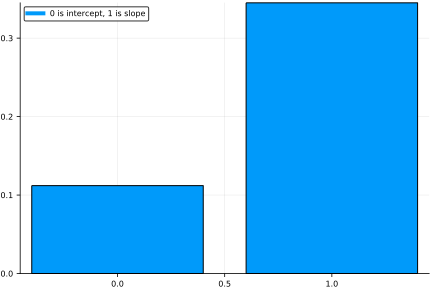
\includegraphics[width=15cm]{Examples/GLS/EffectsOLS}

\end{figure}


\textbf{\newpage{}Summary}: OLS with heteroscedasticity and/or autocorrelation is:
\begin{itemize}
\item unbiased with fixed or strongly exogenous regressors
\item biased with weakly exogenous regressors
\item has a different variance than before, so the previous test statistics aren't valid 
\item is consistent
\item is asymptotically normally distributed, but with a different limiting covariance matrix. Previous test statistics aren't valid in this case for this reason.
\item is inefficient, as is shown below. 
\end{itemize}

\section{The GLS estimator}

Suppose $\Sigma$ were known. Then one could form the Cholesky decomposition
\[
P^{\prime}P=\Sigma^{-1}
\]
 Here, $P$ is an upper triangular matrix. We have 
\[
P^{\prime}P\Sigma=I_{n}
\]
 so 
\[
P^{\prime}P\Sigma P^{\prime}=P^{\prime},
\]
 which implies that 
\[
P\Sigma P^{\prime}=I_{n}
\]


Let's take some time to play with the Cholesky decomposition. Try out the  \htmladdnormallink{GLS/cholesky.m}{file:///home/michael/Mystuff/Econometrics/Examples/GLS/cholesky.m} Octave script to see that the above claims are true, and also to see how one can generate data from a $N(0,V)$ distribition.

Consider the model 
\[
Py=PX\beta+P\varepsilon,
\]
 or, making the obvious definitions, 
\[
y^{*}=X^{*}\beta+\varepsilon^{*}.
\]
 This variance of $\varepsilon^{*}=P\varepsilon$ is 
\begin{eqnarray*}
\mathcal{E}(P\varepsilon\varepsilon^{\prime}P^{\prime}) & = & P\Sigma P^{\prime}\\
 & = & I_{n}
\end{eqnarray*}
 Therefore, the model 
\begin{eqnarray*}
y^{*} & = & X^{*}\beta+\varepsilon^{*}\\
\mathcal{E}(\varepsilon^{*}) & = & 0\\
V(\varepsilon^{*}) & = & I_{n}
\end{eqnarray*}
 satisfies the classical assumptions. The GLS estimator is simply OLS\ applied to the transformed model: 
\begin{eqnarray*}
\hat{\beta}_{GLS} & = & (X^{*\prime}X^{*})^{-1}X^{*\prime}y^{*}\\
 & = & (X^{\prime}P'PX)^{-1}X^{\prime}P'Py\\
 & = & (X^{\prime}\Sigma^{-1}X)^{-1}X^{\prime}\Sigma^{-1}y
\end{eqnarray*}


The GLS\ estimator is unbiased in the same circumstances under which the OLS\ estimator is unbiased. For example, assuming $X$ is nonstochastic 
\begin{eqnarray*}
\mathcal{E}(\hat{\beta}_{GLS}) & = & \mathcal{E}\left\{ (X^{\prime}\Sigma^{-1}X)^{-1}X^{\prime}\Sigma^{-1}y\right\} \\
 & = & \mathcal{E}\left\{ (X^{\prime}\Sigma^{-1}X)^{-1}X^{\prime}\Sigma^{-1}(X\beta+\varepsilon\right\} \\
 & = & \beta.
\end{eqnarray*}
To get the variance of the estimator, we have 
\begin{eqnarray*}
\hat{\beta}_{GLS} & = & (X^{*\prime}X^{*})^{-1}X^{*\prime}y^{*}\\
 & = & (X^{*\prime}X^{*})^{-1}X^{*\prime}\left(X^{*}\beta+\varepsilon^{*}\right)\\
 & = & \beta+(X^{*\prime}X^{*})^{-1}X^{*\prime}\varepsilon^{*}
\end{eqnarray*}
 so 
\begin{eqnarray*}
\mathcal{E}\left\{ \left(\hat{\beta}_{GLS}-\beta\right)\left(\hat{\beta}_{GLS}-\beta\right)^{\prime}\right\}  & = & \mathcal{E}\left\{ (X^{*\prime}X^{*})^{-1}X^{*\prime}\varepsilon^{*}\varepsilon^{*\prime}X^{*}(X^{*\prime}X^{*})^{-1}\right\} \\
 & = & (X^{*\prime}X^{*})^{-1}X^{*\prime}X^{*}(X^{*\prime}X^{*})^{-1}\\
 & = & (X^{*\prime}X^{*})^{-1}\\
 & = & (X^{\prime}\Sigma^{-1}X)^{-1}
\end{eqnarray*}


Either of these last formulas can be used.


\begin{itemize}
\item All the previous results regarding the desirable properties of the least squares estimator hold, when dealing with the transformed model, since the transformed model satisfies the classical assumptions..
\item Tests are valid, using the previous formulas, as long as we substitute $X^{\ast}$ in place of $X.$ Furthermore, any test that involves $\sigma^{2}$ can set it to $1.$ This is preferable to re-deriving the appropriate formulas.
\item The GLS\ estimator is more efficient than the OLS\ estimator. This is a consequence of the Gauss-Markov theorem, since the GLS estimator is based on a model that satisfies the classical assumptions but the OLS estimator is not. To see this directly, note that
\begin{eqnarray*}
Var(\hat{\beta})-Var(\hat{\beta}_{GLS}) & = & (X'X)^{-1}X'\Sigma X(X'X)^{-1}-(X'\Sigma^{-1}X)^{-1}\\
 & = & A\Sigma A^{'}
\end{eqnarray*}
where $A=\left[\left(X^{\prime}X\right)^{-1}X^{\prime}-(X'\Sigma^{-1}X)^{-1}X'\Sigma^{-1}\right].$ This may not seem obvious, but it is true, as you can verify for yourself. Then noting that $A\Sigma A^{'}$ is a quadratic form in a positive definite matrix, we conclude that $A\Sigma A^{'}$ is positive semi-definite, and that GLS is efficient relative to OLS.
\item As one can verify by calculating first order conditions, the GLS\ estimator is the solution to the minimization problem 
\[
\hat{\beta}_{GLS}=\arg\min(y-X\beta)^{\prime}\Sigma^{-1}(y-X\beta)
\]
 so the \emph{metric} $\Sigma^{-1}$ is used to weight the residuals. 
\end{itemize}

\section{Feasible GLS}

The problem is that $\Sigma$ ordinarily isn't known, so this estimator isn't available.
\begin{itemize}
\item Consider the dimension of $\Sigma$ : it's an $n\times n$ matrix with $\left(n^{2}-n\right)/2+n=\left(n^{2}+n\right)/2$ unique elements (remember - it is symmetric, because it's a covariance matrix).
\item The number of parameters to estimate is larger than $n$ and increases faster than $n.$ There's no way to devise an estimator that satisfies a LLN without adding restrictions.
\item The \emph{feasible GLS estimator} is based upon making sufficient assumptions regarding the form of $\Sigma$ so that a consistent estimator can be devised. 
\end{itemize}
Suppose that we \emph{parameterize} $\Sigma$ as a function of $X$ and $\theta$, where $\theta$ may include $\beta$ as well as other parameters, so that 
\[
\Sigma=\Sigma(X,\theta)
\]
 where $\theta$ is of fixed dimension. If we can consistently estimate $\theta,$ we can consistently estimate $\Sigma,$ as long as the elements of $\Sigma(X,\theta)$ are continuous functions of $\theta$ (by the Slutsky theorem). In this case, 
\[
\widehat{\Sigma}=\Sigma(X,\hat{\theta})\overset{p}{\rightarrow}\Sigma(X,\theta)
\]
 If we replace $\Sigma$ in the formulas for the GLS estimator with $\widehat{\Sigma},$ we obtain the FGLS\ estimator. \textbf{The FGLS estimator shares the same asymptotic properties as GLS. These are}
\begin{enumerate}
\item Consistency
\item Asymptotic normality
\item Asymptotic efficiency \emph{if} the errors are normally distributed. (Cramer-Rao).
\item Test procedures are asymptotically valid. 
\end{enumerate}
\textbf{In practice, the usual way to proceed is}
\begin{enumerate}
\item Define a consistent estimator of $\theta.$ This is a case-by-case proposition, depending on the parameterization $\Sigma(\theta).$ We'll see examples below.
\item Form $\widehat{\Sigma}=\Sigma(X,\hat{\theta})$
\item Calculate the Cholesky factorization $\widehat{P}=Chol(\hat{\Sigma}^{-1})$.
\item Transform the model using 
\[
\hat{P}y=\hat{P}X\beta+\hat{P}\varepsilon
\]

\item Estimate using OLS on the transformed model. 
\end{enumerate}

\section{Heteroscedasticity}

Heteroscedasticity is the case where 
\[
\mathcal{E}(\varepsilon\varepsilon^{\prime})=\Sigma
\]
 is a diagonal matrix, so that the errors are uncorrelated, but have different variances. Heteroscedasticity is usually thought of as associated with cross sectional data, though there is absolutely no reason why time series data cannot also be heteroscedastic. Actually, the popular ARCH (autoregressive conditionally heteroscedastic) models explicitly assume that a time series is heteroscedastic.

Consider a supply function 
\[
q_{i}=\beta_{1}+\beta_{p}P_{i}+\beta_{s}S_{i}+\varepsilon_{i}
\]
 where $P_{i}$ is price and $S_{i}$ is some measure of size of the $i^{th}$ firm. One might suppose that unobservable factors (e.g., talent of managers, degree of coordination between production units, \emph{etc.}) account for the error term $\varepsilon_{i}.$ If there is more variability in these factors for large firms than for small firms, then $\varepsilon_{i}$ may have a higher variance when $S_{i}$ is high than when it is low.

Another example, individual demand. 
\[
q_{i}=\beta_{1}+\beta_{p}P_{i}+\beta_{m}M_{i}+\varepsilon_{i}
\]
 where $P$ is price and $M$ is income. In this case, $\varepsilon_{i}$ can reflect variations in preferences. There are more possibilities for expression of preferences when one is rich, so it is possible that the variance of $\varepsilon_{i}$ could be higher when $M$ is high.

\emph{Add example of group means.}


\subsection{OLS with heteroscedastic consistent varcov estimation}

Eicker (1967) and White (1980) showed how to modify test statistics to account for heteroscedasticity of unknown form. The OLS\ estimator has asymptotic distribution 
\[
\sqrt{n}\left(\hat{\beta}-\beta\right)\overset{d}{\rightarrow}N\left(0,Q_{X}^{-1}\Omega Q_{X}^{-1}\right)
\]
 as we've already seen. Recall that we defined 
\[
\lim_{n\rightarrow\infty}\mathcal{E}\left(\frac{X^{\prime}\varepsilon\varepsilon^{\prime}X}{n}\right)=\Omega
\]
 This matrix has dimension $K\times K$ and can be consistently estimated, even if we can't estimate $\Sigma$ consistently. The consistent estimator, under heteroscedasticity but no autocorrelation is 
\[
\widehat{\Omega}=\frac{1}{n}\sum_{t=1}^{n}x_{t}x_{t}^{\prime}\hat{\varepsilon}_{t}^{2}
\]
 One can then modify the previous test statistics to obtain tests that are valid when there is heteroscedasticity of unknown form. For example, the Wald test for $H_{0}:R\beta-r=0$ would be 
\[
n\left(R\hat{\beta}-r\right)^{\prime}\left(R\left(\frac{X^{\prime}X}{n}\right)^{-1}\hat{\Omega}\left(\frac{X^{\prime}X}{n}\right)^{-1}R^{\prime}\right)^{-1}\left(R\hat{\beta}-r\right)\overset{a}{\sim}\chi^{2}(q)
\]


To see the effects of ignoring HET when doing OLS, and the good effect of using a HET consistent covariance estimator, consider the script  \htmladdnormallink{bootstrap\_example1.m}{file:///home/michael/Mystuff/Econometrics/Examples/Parallel/bootstrap/bootstrap\_example1.m}. This script generates data from a linear model with HET, then computes standard errors using the ordinary OLS formula, the Eicker-White formula, and also bootstrap standard errors. Note that Eicker-White and bootstrap pretty much agree, while the OLS formula gives standard errors that are quite different. Typical output of this script follows:\newpage{} \verbatiminput{Examples/Parallel/bootstrap/bootstrap_example1.out}
\begin{itemize}
\item If you run this several times, you will notice that the OLS standard error for the last parameter appears to be biased downward, at least comparing to the other two methods, which are asymptotically valid.
\item The true coefficients \emph{are} zero. With a standard error biased downward, the t-test for lack of significance will reject more often than it should (the variables really are not significant, but we will find that they seem to be more often than is due to Type-I error.
\item For example, you should see that the p-value for the last coefficient is smaller than 0.10 more than 10\% of the time. Run the script 20 times and you'll see.
\end{itemize}

\subsection{Detection}

There exist many tests for the presence of heteroscedasticity. We'll discuss three methods.


\paragraph{Goldfeld-Quandt}

The sample is divided in to three parts, with $n_{1},n_{2}$ and $n_{3}$ observations, where $n_{1}+n_{2}+n_{3}=n$. The model is estimated using the first and third parts of the sample, separately, so that $\hat{\beta}^{1}$ and $\hat{\beta}^{3}$ will be independent. Then we have 
\[
\frac{\hat{\varepsilon}^{1\prime}\hat{\varepsilon}^{1}}{\sigma^{2}}=\frac{\varepsilon^{1^{\prime}}M^{1}\varepsilon^{1}}{\sigma^{2}}\overset{d}{\rightarrow}\chi^{2}(n_{1}-K)
\]
 and

\[
\frac{\hat{\varepsilon}^{3\prime}\hat{\varepsilon}^{3}}{\sigma^{2}}=\frac{\varepsilon^{3^{\prime}}M^{3}\varepsilon^{3}}{\sigma^{2}}\overset{d}{\rightarrow}\chi^{2}(n_{3}-K)
\]
 so 
\[
\frac{\hat{\varepsilon}^{1\prime}\hat{\varepsilon}^{1}/(n_{1}-K)}{\hat{\varepsilon}^{3\prime}\hat{\varepsilon}^{3}/(n_{3}-K)}\overset{d}{\rightarrow}F(n_{1}-K,n_{3}-K).
\]
 The distributional result is exact if the errors are normally distributed. This test is a two-tailed test. Alternatively, and probably more conventionally, if one has prior ideas about the possible magnitudes of the variances of the observations, one could order the observations accordingly, from largest to smallest. In this case, one would use a conventional one-tailed F-test. \emph{Draw picture.}
\begin{itemize}
\item Ordering the observations is an important step if the test is to have any power.
\item The motive for dropping the middle observations is to increase the difference between the average variance in the subsamples, supposing that there exists heteroscedasticity. This can increase the power of the test. On the other hand, dropping too many observations will substantially increase the variance of the statistics $\hat{\varepsilon}^{1\prime}\hat{\varepsilon}^{1}$ and $\hat{\varepsilon}^{3\prime}\hat{\varepsilon}^{3}.$ A rule of thumb, based on Monte Carlo experiments is to drop around 25\% of the observations.
\item If one doesn't have any ideas about the form of the het. the test will probably have low power since a sensible data ordering isn't available. 
\end{itemize}

\paragraph{White's test}

When one has little idea if there exists heteroscedasticity, and no idea of its potential form, the White test is a possibility. The idea is that if there is homoscedasticity, then 
\[
\mathcal{E}(\varepsilon_{t}^{2}|x_{t})=\sigma^{2},\forall t
\]
 so that $x_{t}$ or functions of $x_{t}$ shouldn't help to explain $\mathcal{E}(\varepsilon_{t}^{2}).$ The test works as follows:
\begin{enumerate}
\item Since $\varepsilon_{t}$ isn't available, use the consistent estimator $\hat{\varepsilon}_{t}$ instead.
\item Regress 
\[
\hat{\varepsilon}_{t}^{2}=\sigma^{2}+z_{t}^{\prime}\gamma+v_{t}
\]
 where $z_{t}$ is a $P$-vector. $z_{t}$ may include some or all of the variables in $x_{t},$ as well as other variables. White's original suggestion was to use $x_{t}$, plus the set of all unique squares and cross products of variables in $x_{t}.$
\item Test the hypothesis that $\gamma=0.$ The $qF$ statistic in this case is 
\[
qF=\frac{P\left(ESS_{R}-ESS_{U}\right)/P}{ESS_{U}/\left(n-P-1\right)}
\]
 Note that $ESS_{R}=TSS_{U},$ so dividing both numerator and denominator by this we get 
\[
qF=\left(n-P-1\right)\frac{R^{2}}{1-R^{2}}
\]
 Note that this is the $R^{2}$ of the artificial regression used to test for heteroscedasticity, not the $R^{2}$ of the original model. 
\end{enumerate}
An asymptotically equivalent statistic, under the null of no heteroscedasticity (so that $R^{2}$ should tend to zero), is

\[
nR^{2}\overset{a}{\sim}\chi^{2}(P).
\]
 This doesn't require normality of the errors, though it does assume that the fourth moment of $\varepsilon_{t}$ is constant, under the null. \textbf{Question}: why is this necessary?
\begin{itemize}
\item The White test has the disadvantage that it may not be very powerful unless the $z_{t}$ vector is chosen well, and this is hard to do without knowledge of the form of heteroscedasticity.
\item It also has the problem that specification errors other than heteroscedasticity may lead to rejection.
\item Note: the null hypothesis of this test may be interpreted as $\theta=0$ for the variance model $V(\varepsilon_{t}^{2})=h(\alpha+z_{t}^{\prime}\theta),$ where $h(\cdot)$ is an arbitrary function of unknown form. The test is more general than is may appear from the regression that is used.
\end{itemize}

\paragraph{Plotting the residuals}

A very simple method is to simply plot the residuals (or their squares). \emph{Draw pictures here}. Like the Goldfeld-Quandt test, this will be more informative if the observations are ordered according to the suspected form of the heteroscedasticity.


\subsection{Correction}

Correcting for heteroscedasticity requires that a parametric form for $\Sigma(\theta)$ be supplied, and that a means for estimating $\theta$ consistently be determined. The estimation method will be specific to the for supplied for $\Sigma(\theta).$ We'll consider two examples. Before this, let's consider the general nature of GLS\ when there is heteroscedasticity. 

When we have HET but no AUT, $\Sigma$ is a diagonal matrix:
\[
\Sigma=\left[\begin{array}{cccc}
\sigma_{1}^{2} & 0 & \ldots & 0\\
\vdots & \sigma_{2}^{2} &  & \vdots\\
 &  & \ddots & 0\\
0 & \cdots & 0 & \sigma_{n}^{2}
\end{array}\right]
\]
Likewise, $\Sigma^{-1}$ is diagonal
\[
\Sigma^{-1}=\left[\begin{array}{cccc}
\frac{1}{\sigma_{1}^{2}} & 0 & \ldots & 0\\
\vdots & \frac{1}{\sigma_{2}^{2}} &  & \vdots\\
 &  & \ddots & 0\\
0 & \cdots & 0 & \frac{1}{\sigma_{n}^{2}}
\end{array}\right]
\]
and so is the Cholesky decomposition $P=chol(\Sigma^{-1}$)
\[
P=\left[\begin{array}{cccc}
\frac{1}{\sigma_{1}} & 0 & \ldots & 0\\
\vdots & \frac{1}{\sigma_{2}} &  & \vdots\\
 &  & \ddots & 0\\
0 & \cdots & 0 & \frac{1}{\sigma_{n}}
\end{array}\right]
\]
 We need to transform the model, just as before, in the general case: 
\[
Py=PX\beta+P\varepsilon,
\]
 or, making the obvious definitions, 
\[
y^{*}=X^{*}\beta+\varepsilon^{*}.
\]
 Note that multiplying by $P$ just divides the data for each observation ($y_{i},x_{i})$ by the corresponding standard error of the error term, $\sigma_{i}$. That is, $y_{i}^{*}=y_{i}/\sigma_{i}$ and $x_{i}^{*}=x_{i}/\sigma_{i}$ (note that $x_{i}$ is a $K$-vector: we divided each element, including the 1 corresponding to the constant).

This makes sense. Consider Figure \ref{fig:Motivation-for-GLS}, which shows a true regression line with heteroscedastic errors. Which sample is more informative about the location of the line? The ones with observations with smaller variances. So, the GLS solution is equivalent to OLS on the transformed data. By the transformed data is the original data, weighted by the inverse of the standard error of the observation's error term. When the standard error is small, the weight is high, and vice versa. The GLS correction for the case of HET is also known as weighted least squares, for this reason.

\begin{figure}
\caption{\label{fig:Motivation-for-GLS}Motivation for GLS correction when there is HET}


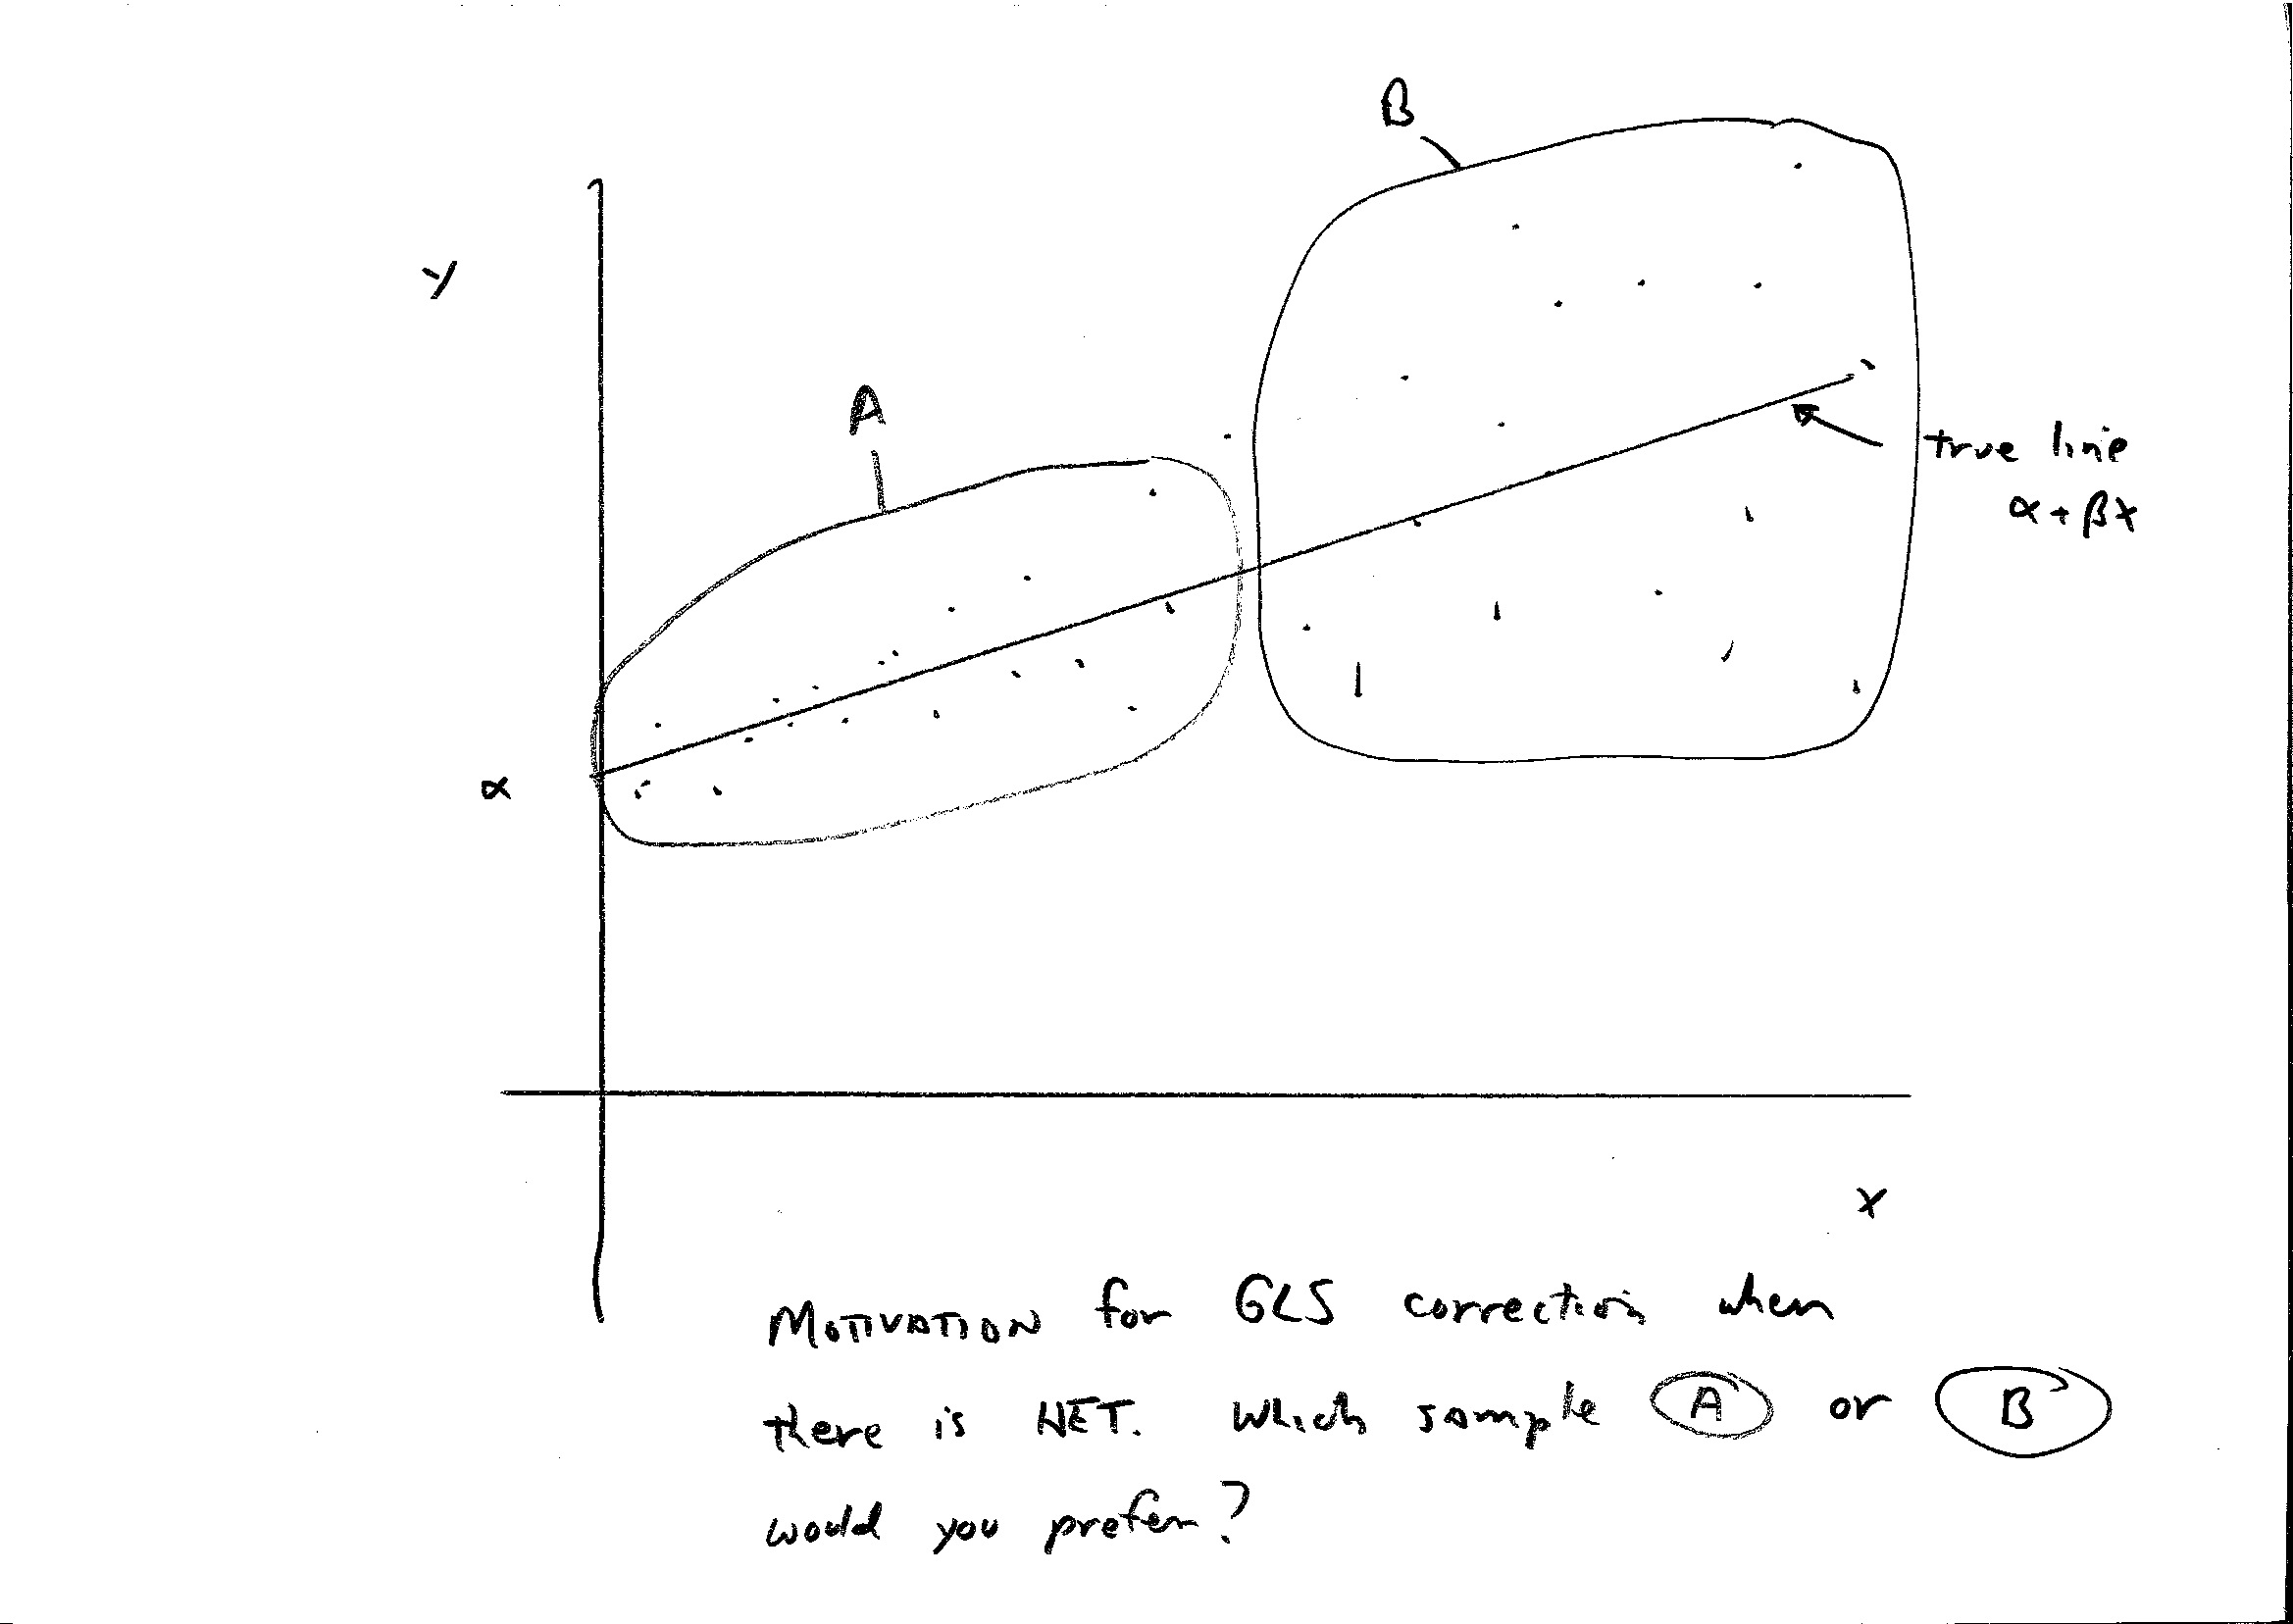
\includegraphics[width=15cm]{Examples/GLS/wls}
\end{figure}



\subsubsection{Multiplicative heteroscedasticity}

Suppose the model is 
\begin{eqnarray*}
y_{t} & = & x_{t}^{\prime}\beta+\varepsilon_{t}\\
\sigma_{t}^{2} & = & \mathcal{E}(\varepsilon_{t}^{2})=\left(z_{t}^{\prime}\gamma\right)^{\delta}
\end{eqnarray*}
 but the other classical assumptions hold. In this case 
\[
\varepsilon_{t}^{2}=\left(z_{t}^{\prime}\gamma\right)^{\delta}+v_{t}
\]
 and $v_{t}$ has mean zero. Nonlinear least squares could be used to estimate $\gamma$ and $\delta$ consistently, were $\varepsilon_{t}$ observable. The solution is to substitute the squared OLS residuals $\hat{\varepsilon}_{t}^{2}$ in place of $\varepsilon_{t}^{2},$ since it is consistent by the Slutsky theorem. Once we have $\hat{\gamma}$ and $\hat{\delta},$ we can estimate $\sigma_{t}^{2}$ consistently using 
\[
\hat{\sigma}_{t}^{2}=\left(z_{t}^{\prime}\hat{\gamma}\right)^{\hat{\delta}}\overset{p}{\rightarrow\sigma_{t}^{2}}.
\]
 In the second step, we transform the model by dividing by the standard deviation: 
\[
\frac{y_{t}}{\hat{\sigma}_{t}}=\frac{x_{t}^{\prime}\beta}{\hat{\sigma}_{t}}+\frac{\varepsilon_{t}}{\hat{\sigma}_{t}}
\]
 or 
\[
y_{t}^{*}=x_{t}^{*\prime}\beta+\varepsilon_{t}^{*}.
\]
 Asymptotically, this model satisfies the classical assumptions.
\begin{itemize}
\item This model is a bit complex in that NLS\ is required to estimate the model of the variance. A simpler version would be 
\begin{eqnarray*}
y_{t} & = & x_{t}^{\prime}\beta+\varepsilon_{t}\\
\sigma_{t}^{2} & =\mathcal{E}(\varepsilon_{t}^{2})= & \sigma^{2}z_{t}^{\delta}
\end{eqnarray*}
 where $z_{t}$ is a single variable. There are still two parameters to be estimated, and the model of the variance is still nonlinear in the parameters. However, the \emph{search method} can be used in this case to reduce the estimation problem to repeated applications of OLS.
\item First, we define an interval of reasonable values for $\delta,$ e.g., $\delta\in[0,3].$
\item Partition this interval into $M$ equally spaced values, e.g., $\{0,.1,.2,...,2.9,3\}.$
\item For each of these values, calculate the variable $z_{t}^{\delta_{m}}.$
\item The regression 
\[
\hat{\varepsilon}_{t}^{2}=\sigma^{2}z_{t}^{\delta_{m}}+v_{t}
\]
 is linear in the parameters, conditional on $\delta_{m},$ so one can estimate $\sigma^{2}$ by OLS.
\item Save the pairs ($\sigma_{m}^{2},\delta_{m}),$ and the corresponding $ESS_{m}.$ Choose the pair with the minimum $ESS_{m}$ as the estimate. 
\item Next, divide the model by the estimated standard deviations.
\item Can refine. \emph{Draw picture. }
\item Works well when the parameter to be searched over is low dimensional, as in this case. 
\end{itemize}

\subsubsection{Groupwise heteroscedasticity}

A common case is where we have repeated observations on each of a number of economic agents: e.g., 10 years of macroeconomic data on each of a set of countries or regions, or daily observations of transactions of 200 banks. This sort of data is a \emph{pooled cross-section time-series model.} It may be reasonable to presume that the variance is constant over time within the cross-sectional units, but that it differs across them (e.g., firms or countries of different sizes...). The model is 
\begin{eqnarray*}
y_{it} & = & x_{it}^{\prime}\beta+\varepsilon_{it}\\
\mathcal{E}(\varepsilon_{it}^{2}) & = & \sigma_{i}^{2},\forall t
\end{eqnarray*}
 where $i=1,2,...,G$ are the agents, and $t=1,2,...,n$ are the observations on each agent.
\begin{itemize}
\item The other classical assumptions are presumed to hold.
\item In this case, the variance $\sigma_{i}^{2}$ is specific to each agent, but constant over the $n$ observations for that agent.
\item In this model, we assume that $\mathcal{E}(\varepsilon_{it}\varepsilon_{is})=0.$ This is a strong assumption that we'll relax later. 
\end{itemize}
To correct for heteroscedasticity, just estimate each $\sigma_{i}^{2}$ using the natural estimator: 
\[
\hat{\sigma}_{i}^{2}=\frac{1}{n}\sum_{t=1}^{n}\hat{\varepsilon}_{it}^{2}
\]

\begin{itemize}
\item Note that we use $1/n$ here since it's possible that there are more than $n$ regressors, so $n-K$ could be negative. Asymptotically the difference is unimportant.
\item With each of these, transform the model as usual: 
\[
\frac{y_{it}}{\hat{\sigma}_{i}}=\frac{x_{it}^{\prime}\beta}{\hat{\sigma}_{i}}+\frac{\varepsilon_{it}}{\hat{\sigma}_{i}}
\]
 Do this for each cross-sectional group. This transformed model satisfies the classical assumptions, asymptotically. 
\end{itemize}

\subsection{Example: the Nerlove model (again!)\label{sub:Nerlove GLS by groups}}

Remember the Nerlove data - see sections \ref{sec:Example:-The-Nerlove} and \ref{sec:Example: Nerlove restrictions}. Let's check the Nerlove data for evidence of heteroscedasticity. In what follows, we're going to use the model with the constant and output coefficient varying across 5 groups, but with the input price coefficients fixed (see Equation \ref{Nerlove, favorite model} for the rationale behind this). Figure \ref{cap:Residuals,-Nerlove-model,}, which is generated by the Octave program  \htmladdnormallink{GLS/NerloveResiduals.m}{file:///home/michael/Mystuff/Econometrics/Examples/GLS/NerloveResiduals.m} plots the residuals. We can see pretty clearly that the error variance is larger for small firms than for larger firms. 
\begin{figure}
\caption{\label{cap:Residuals,-Nerlove-model,}Residuals, Nerlove model, sorted by firm size}


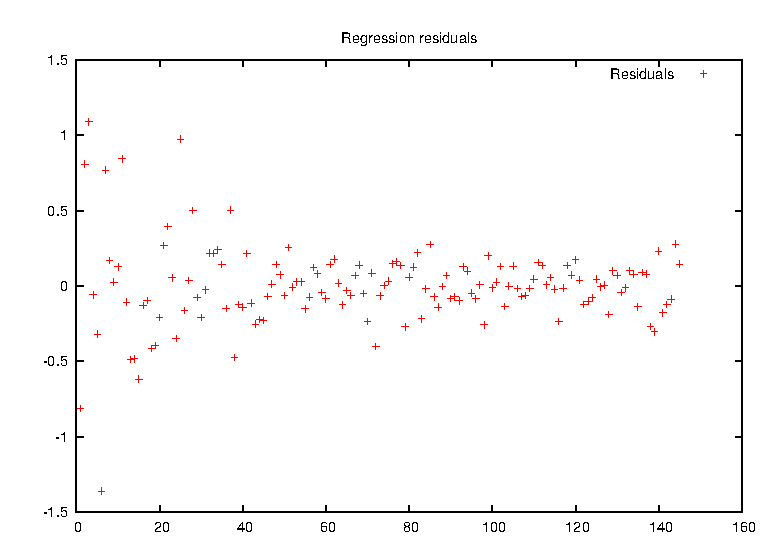
\includegraphics{Examples/GLS/NerloveResiduals}
\end{figure}


Now let's try out some tests to formally check for heteroscedasticity. The Octave program  \htmladdnormallink{GLS/HetTests.m}{file:///home/michael/Mystuff/Econometrics/Examples/GLS/HetTests.m} performs the White and Goldfeld-Quandt tests, using the above model. The results are\verbatiminput{Examples/GLS/HetTests.out}All in all, it is very clear that the data are heteroscedastic. That means that OLS estimation is not efficient, and tests of restrictions that ignore heteroscedasticity are not valid. The previous tests (CRTS, HOD1 and the Chow test) were calculated assuming homoscedasticity. The Octave program  \htmladdnormallink{GLS/NerloveRestrictions-Het.m}{file:///home/michael/Mystuff/Econometrics/Examples/GLS/NerloveRestrictionsHet.m} uses the Wald test to check for CRTS and HOD1, but using a heteroscedastic-consistent covariance estimator.\footnote{By the way, notice that  \htmladdnormallink{GLS/NerloveResiduals.m}{file:///home/michael/Mystuff/Econometrics/Examples/GLS/NerloveResiduals.m} and  \htmladdnormallink{GLS/HetTests.m}{file:///home/michael/Mystuff/Econometrics/Examples/GLS/HetTests.m} use the restricted LS estimator directly to restrict the fully general model with all coefficients varying to the model with only the constant and the output coefficient varying. But  \htmladdnormallink{GLS/NerloveRestrictions-Het.m}{file:///home/michael/Mystuff/Econometrics/Examples/GLS/NerloveRestrictions-Het.m} estimates the model by substituting the restrictions into the model. The methods are equivalent, but the second is more convenient and easier to understand.} The results are\verbatiminput{Examples/GLS/CRTS_HOD1.out}We see that the previous conclusions are altered - both CRTS is and HOD1 are rejected at the 5\% level. Maybe the rejection of HOD1 is due to to Wald test's tendency to over-reject? 

From the previous plot, it seems that the variance of $\epsilon$ is a decreasing function of output. Suppose that the 5 size groups have different error variances (heteroscedasticity by groups):
\[
Var(\epsilon_{i})=\sigma_{j}^{2},
\]
where $j=1$ if $i=1,2,...,29$, \emph{etc.,} as before. The Octave script  \htmladdnormallink{GLS/NerloveGLS.m}{file:///home/michael/Mystuff/Econometrics/Examples/GLS/NerloveGLS.m} estimates the model using GLS (through a transformation of the model so that OLS can be applied). The estimation results are i\verbatiminput{Examples/GLS/NerloveGLS.out}The first panel of output are the OLS estimation results, which are used to consistently estimate the $\sigma_{j}^{2}$. The second panel of results are the GLS estimation results. Some comments:
\begin{itemize}
\item The $R^{2}$ measures are not comparable - the dependent variables are not the same. The measure for the GLS results uses the transformed dependent variable. One could calculate a comparable $R^{2}$ measure, but I have not done so.
\item The differences in estimated standard errors (smaller in general for GLS) \emph{can} be interpreted as evidence of improved efficiency of GLS, since the OLS standard errors are calculated using the Huber-White estimator. They would not be comparable if the ordinary (inconsistent) estimator had been used.
\item Note that the previously noted pattern in the output coefficients persists. The nonconstant CRTS result is robust.
\item The coefficient on capital is now negative and significant at the 3\% level. That seems to indicate some kind of problem with the model or the data, or economic theory.
\item Note that HOD1 is now rejected. Problem of Wald test over-rejecting? Specification error in model? 
\end{itemize}

\section{Autocorrelation}

Autocorrelation, which is the serial correlation of the error term, is a problem that is usually associated with time series data, but also can affect cross-sectional data. For example, a shock to oil prices will simultaneously affect all countries, so one could expect contemporaneous correlation of macroeconomic variables across countries.


\subsection{Example}

Consider the Keeling-Whorf data on atmospheric CO2 concentrations an Mauna Loa, Hawaii (see \url{http://en.wikipedia.org/wiki/Keeling_Curve} and \url{http://cdiac.ornl.gov/ftp/ndp001/maunaloa.txt}).

From the file maunaloa.txt: ''THE DATA FILE PRESENTED IN THIS SUBDIRECTORY CONTAINS MONTHLY AND ANNUAL ATMOSPHERIC CO2 CONCENTRATIONS DERIVED FROM THE SCRIPPS INSTITUTION OF OCEANOGRAPHY'S (SIO's) CONTINUOUS MONITORING PROGRAM AT MAUNA LOA OBSERVATORY, HAWAII. THIS RECORD CONSTITUTES THE LONGEST CONTINUOUS RECORD OF ATMOSPHERIC CO2 CONCENTRATIONS AVAILABLE IN THE WORLD. MONTHLY AND ANNUAL AVERAGE MOLE FRACTIONS OF CO2 IN WATER-VAPOR-FREE AIR ARE GIVEN FROM MARCH 1958 THROUGH DECEMBER 2003, EXCEPT FOR A FEW INTERRUPTIONS.'' \newpage{}

The data is available in Octave format at  \htmladdnormallink{CO2.data}{file:///home/michael/Mystuff/Econometrics/Examples/Data/CO2.data} . 

If we fit the model $CO2_{t}=\beta_{1}+\beta_{2}t+\epsilon_{t}$, we get the results\verbatiminput{Examples/GLS/CO2Example.out}It seems pretty clear that CO2 concentrations have been going up in the last 50 years, surprise, surprise. Let's look at a residual plot for the last 3 years of the data, see Figure \ref{fig:Residuals-from-time}. Note that there is a very predictable pattern. This is pretty strong evidence that the errors of the model are not independent of one another, which means there seems to be autocorrelation.

\begin{figure}
\caption{\label{fig:Residuals-from-time}Residuals from time trend for CO2 data}


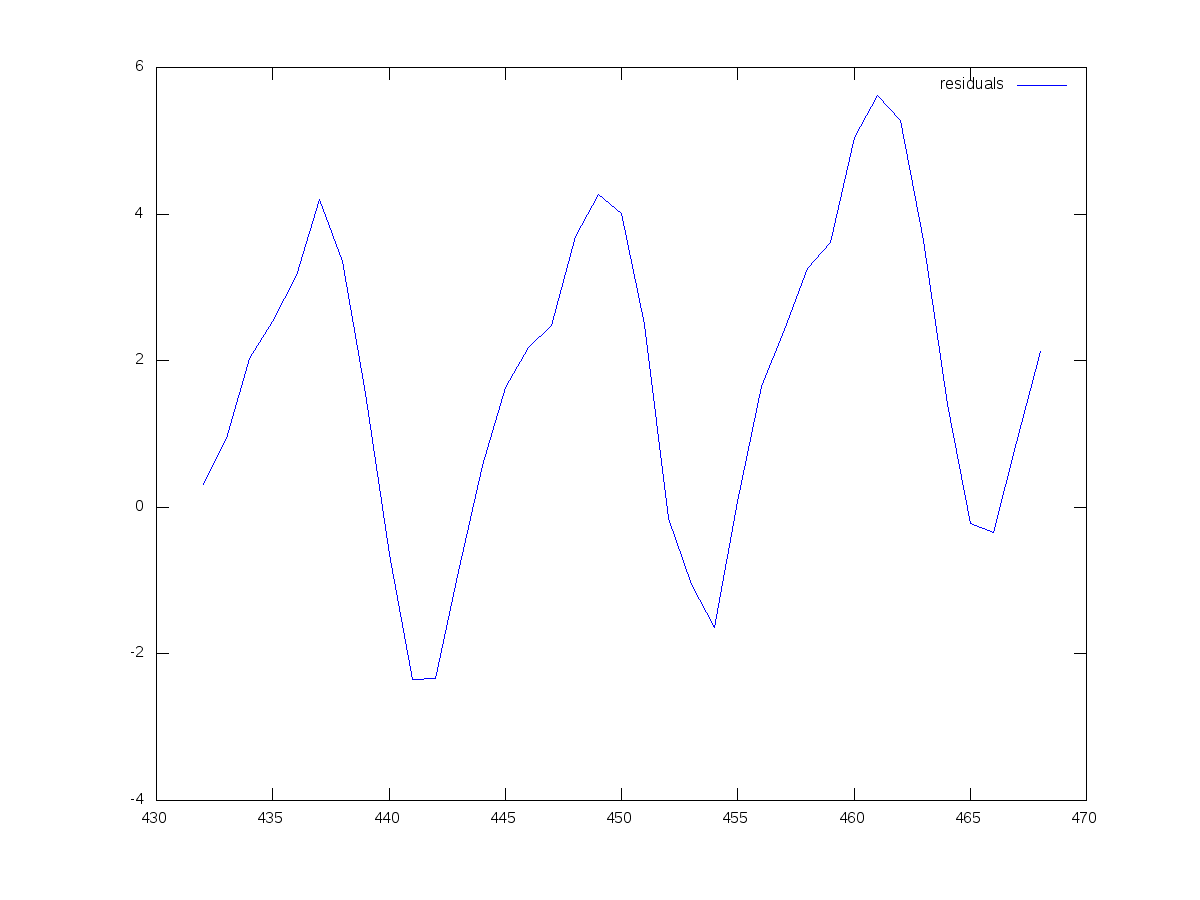
\includegraphics[width=15cm]{Examples/GLS/CO2Residuals}

\end{figure}



\subsection{Causes}

Autocorrelation is the existence of correlation across the error term: 
\[
\mathcal{E}(\varepsilon_{t}\varepsilon_{s})\neq0,t\neq s.
\]
 Why might this occur? Plausible explanations include
\begin{enumerate}
\item Lags in adjustment to shocks. In a model such as 
\[
y_{t}=x_{t}^{\prime}\beta+\varepsilon_{t},
\]
 one could interpret $x_{t}^{\prime}\beta$ as the equilibrium value. Suppose $x_{t}$ is constant over a number of observations. One can interpret $\varepsilon_{t}$ as a shock that moves the system away from equilibrium. If the time needed to return to equilibrium is long with respect to the observation frequency, one could expect $\varepsilon_{t+1}$ to be positive, conditional on $\varepsilon_{t}$ positive, which induces a correlation.
\item Unobserved factors that are correlated over time. The error term is often assumed to correspond to unobservable factors. If these factors are correlated, there will be autocorrelation.
\item Misspecification of the model. Suppose that the DGP is 
\[
y_{t}=\beta_{0}+\beta_{1}x_{t}+\beta_{2}x_{t}^{2}+\varepsilon_{t}
\]
 but we estimate 
\[
y_{t}=\beta_{0}+\beta_{1}x_{t}+\varepsilon_{t}
\]
 The effects are illustrated in Figure \ref{cap:Autocorrelation-induced-by}. 
\begin{figure}
\caption{\label{cap:Autocorrelation-induced-by}Autocorrelation induced by misspecification}


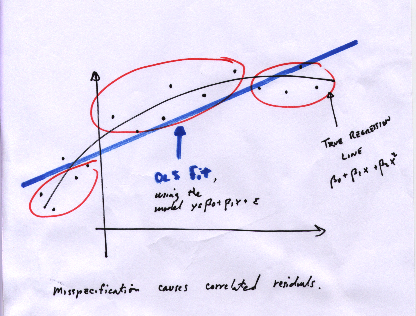
\includegraphics{/home/michael/Mystuff/Econometrics/Examples/Figures/MisspecCausesAutcorrelation}
\end{figure}

\end{enumerate}

\subsection{Effects on the OLS estimator}

The variance of the OLS estimator is the same as in the case of heteroscedasticity - the standard formula does not apply. The correct formula is given in equation \ref{OLS covariance with nonspaerical}. Next we discuss two GLS corrections for OLS. These will potentially induce inconsistency when the regressors are nonstochastic (see Chapter \ref{cha:Stochastic-regressors}) and should either not be used in that case (which is usually the relevant case) or used with caution. The more recommended procedure is discussed in section \ref{sub:Asymptotically-valid-inferences}.


\subsection{AR(1)}

There are many types of autocorrelation. We'll consider two examples. The first is the most commonly encountered case: autoregressive order 1 (AR(1) errors. The model is 
\begin{eqnarray*}
y_{t} & = & x_{t}^{\prime}\beta+\varepsilon_{t}\\
\varepsilon_{t} & = & \rho\varepsilon_{t-1}+u_{t}\\
u_{t} & \sim & iid(0,\sigma_{u}^{2})\\
\mathcal{E}(\varepsilon_{t}u_{s}) & = & 0,t<s
\end{eqnarray*}
 We assume that the model satisfies the other classical assumptions.
\begin{itemize}
\item We need a stationarity assumption: $|\rho|<1.$ Otherwise the variance of $\varepsilon_{t}$ explodes as $t$ increases, so standard asymptotics will not apply.
\item By recursive substitution we obtain 
\begin{eqnarray*}
\varepsilon_{t} & = & \rho\varepsilon_{t-1}+u_{t}\\
 & = & \rho\left(\rho\varepsilon_{t-2}+u_{t-1}\right)+u_{t}\\
 & = & \rho^{2}\varepsilon_{t-2}+\rho u_{t-1}+u_{t}\\
 & = & \rho^{2}\left(\rho\varepsilon_{t-3}+u_{t-2}\right)+\rho u_{t-1}+u_{t}
\end{eqnarray*}
 In the limit the lagged $\varepsilon$ drops out, since $\rho^{m}\rightarrow0$ as $m\rightarrow\infty,$ so we obtain 
\[
\varepsilon_{t}=\sum_{m=0}^{\infty}\rho^{m}u_{t-m}
\]
 With this, the variance of $\varepsilon_{t}$ is found as 
\begin{eqnarray*}
\mathcal{E}(\varepsilon_{t}^{2}) & = & \sigma_{u}^{2}\sum_{m=0}^{\infty}\rho^{2m}\\
 & = & \frac{\sigma_{u}^{2}}{1-\rho^{2}}
\end{eqnarray*}

\item If we had directly assumed that $\varepsilon_{t}$ were covariance stationary, we could obtain this using 
\begin{eqnarray*}
V(\varepsilon_{t}) & = & \rho^{2}\mathcal{E}(\varepsilon_{t-1}^{2})+2\rho\mathcal{E}(\varepsilon_{t-1}u_{t})+\mathcal{E}(u_{t}^{2})\\
 & = & \rho^{2}V(\varepsilon_{t})+\sigma_{u}^{2},
\end{eqnarray*}
 so 
\[
V(\varepsilon_{t})=\frac{\sigma_{u}^{2}}{1-\rho^{2}}
\]

\item The variance is the $0^{th}$ order autocovariance: $\gamma_{0}=V(\varepsilon_{t})$
\item Note that the variance does not depend on $t$
\end{itemize}
Likewise, the first order autocovariance $\gamma_{1}$ is 
\begin{eqnarray*}
Cov(\varepsilon_{t},\varepsilon_{t-1}) & =\gamma_{s}= & \mathcal{E}(\left(\rho\varepsilon_{t-1}+u_{t}\right)\varepsilon_{t-1})\\
 & = & \rho V(\varepsilon_{t})\\
 & = & \frac{\rho\sigma_{u}^{2}}{1-\rho^{2}}
\end{eqnarray*}

\begin{itemize}
\item Using the same method, we find that for $s<t$
\[
Cov(\varepsilon_{t},\varepsilon_{t-s})=\gamma_{s}=\frac{\rho^{s}\sigma_{u}^{2}}{1-\rho^{2}}
\]

\item The autocovariances don't depend on $t$: the process $\{\varepsilon_{t}\}$ is \emph{covariance stationary}
\end{itemize}
The \emph{correlation (}in general, for r.v.'s $x$ and $y$) is defined as 
\[
\text{corr}(x,y)=\frac{\text{cov}(x,y)}{\text{se}(x)\text{se}(y)}
\]
 but in this case, the two standard errors are the same, so the $s$-order autocorrelation $\rho_{s}$ is 
\[
\rho_{s}=\rho^{s}
\]

\begin{itemize}
\item All this means that the overall matrix $\Sigma$ has the form 
\[
\Sigma=\underbrace{\frac{\sigma_{u}^{2}}{1-\rho^{2}}}_{\textrm{this is the variance}}\underbrace{\left[\begin{array}{ccccc}
1 & \rho & \rho^{2} & \cdots & \rho^{n-1}\\
\rho & 1 & \rho & \cdots & \rho^{n-2}\\
\vdots &  & \ddots &  & \vdots\\
 &  &  & \ddots & \rho\\
\rho^{n-1} & \cdots &  &  & 1
\end{array}\right]}_{\textrm{this is the correlation matrix}}
\]
 So we have homoscedasticity, but elements off the main diagonal are not zero. All of this depends only on two parameters, $\rho$ and $\sigma_{u}^{2}.$ If we can estimate these consistently, we can apply FGLS. 
\end{itemize}
It turns out that it's easy to estimate these consistently. The steps are
\begin{enumerate}
\item Estimate the model $y_{t}=x_{t}^{\prime}\beta+\varepsilon_{t}$ by OLS.
\item Take the residuals, and estimate the model 
\[
\hat{\varepsilon}_{t}=\rho\hat{\varepsilon}_{t-1}+u_{t}^{*}
\]
 Since $\hat{\varepsilon}_{t}\overset{p}{\rightarrow}\varepsilon_{t},$ this regression is asymptotically equivalent to the regression 
\[
\varepsilon_{t}=\rho\varepsilon_{t-1}+u_{t}
\]
 which satisfies the classical assumptions. Therefore, $\hat{\rho}$ obtained by applying OLS to $\hat{\varepsilon}_{t}=\rho\hat{\varepsilon}_{t-1}+u_{t}^{*}$ is consistent. Also, since $u_{t}^{*}\overset{p}{\rightarrow}u_{t}$, the estimator 
\[
\hat{\sigma}_{u}^{2}=\frac{1}{n}\sum_{t=2}^{n}\left(\hat{u}_{t}^{*}\right)^{2}\overset{p}{\rightarrow}\sigma_{u}^{2}
\]

\item With the consistent estimators $\hat{\sigma}_{u}^{2}$ and $\hat{\rho},$ form $\hat{\Sigma}=\Sigma(\hat{\sigma}_{u}^{2},\hat{\rho})$ using the previous structure of $\Sigma,$ and estimate by FGLS. Actually, one can omit the factor $\hat{\sigma}_{u}^{2}/(1-\rho^{2}),$ since it cancels out in the formula 
\[
\hat{\beta}_{FGLS}=\left(X^{\prime}\hat{\Sigma}^{-1}X\right)^{-1}(X^{\prime}\hat{\Sigma}^{-1}y).
\]
\end{enumerate}
\begin{itemize}
\item One can iterate the process, by taking the first FGLS estimator of $\beta,$ re-estimating $\rho$ and $\sigma_{u}^{2},$ etc. If one iterates to convergences it's equivalent to MLE (supposing normal errors).
\item An asymptotically equivalent approach is to simply estimate the transformed model 
\[
y_{t}-\hat{\rho}y_{t-1}=(x_{t}-\hat{\rho}x_{t-1})^{\prime}\beta+u_{t}^{*}
\]
 using $n-1$ observations (since $y_{0}$ and $x_{0}$ aren't available). This is the method of Cochrane and Orcutt. Dropping the first observation is asymptotically irrelevant, but \emph{it can be very important in small samples.} One can recuperate the first observation by putting 
\begin{eqnarray*}
y_{1}^{*} & =y_{1} & \sqrt{1-\hat{\rho}^{2}}\\
x_{1}^{*} & =x_{1} & \sqrt{1-\hat{\rho}^{2}}
\end{eqnarray*}
 This somewhat odd-looking result is related to the Cholesky factorization of $\Sigma^{-1}.$ See Davidson and MacKinnon, pg. 348-49 for more discussion. Note that the variance of $y_{1}^{*}$ is $\sigma_{u}^{2},$ asymptotically, so we see that the transformed model will be homoscedastic (and nonautocorrelated, since the $u^{\prime}s$ are uncorrelated with the $y^{\prime}s,$ in different time periods. 
\end{itemize}

\subsection{MA(1)}

The linear regression model with moving average order 1 errors is 
\begin{eqnarray*}
y_{t} & = & x_{t}^{\prime}\beta+\varepsilon_{t}\\
\varepsilon_{t} & = & u_{t}+\phi u_{t-1}\\
u_{t} & \sim & iid(0,\sigma_{u}^{2})\\
\mathcal{E}(\varepsilon_{t}u_{s}) & = & 0,t<s
\end{eqnarray*}
 In this case, 
\begin{eqnarray*}
V(\varepsilon_{t}) & =\gamma_{0}= & \mathcal{E}\left[\left(u_{t}+\phi u_{t-1}\right)^{2}\right]\\
 & = & \sigma_{u}^{2}+\phi^{2}\sigma_{u}^{2}\\
 & = & \sigma_{u}^{2}(1+\phi^{2})
\end{eqnarray*}
 Similarly 
\begin{eqnarray*}
\gamma_{1} & = & \mathcal{E}\left[\left(u_{t}+\phi u_{t-1}\right)\left(u_{t-1}+\phi u_{t-2}\right)\right]\\
 & = & \phi\sigma_{u}^{2}
\end{eqnarray*}
 and 
\begin{eqnarray*}
\gamma_{2} & = & \left[\left(u_{t}+\phi u_{t-1}\right)\left(u_{t-2}+\phi u_{t-3}\right)\right]\\
 & = & 0
\end{eqnarray*}
 so in this case 
\[
\Sigma=\sigma_{u}^{2}\left[\begin{array}{ccccc}
1+\phi^{2} & \phi & 0 & \cdots & 0\\
\phi & 1+\phi^{2} & \phi\\
0 & \phi & \ddots &  & \vdots\\
\vdots &  &  & \ddots & \phi\\
0 & \cdots &  & \phi & 1+\phi^{2}
\end{array}\right]
\]
 Note that the first order autocorrelation is 
\begin{eqnarray*}
\rho_{1} & =\frac{\phi\sigma_{u}^{2}}{\sigma_{u}^{2}(1+\phi^{2})} & =\frac{\gamma_{1}}{\gamma_{0}}\\
 & = & \frac{\phi}{(1+\phi^{2})}
\end{eqnarray*}

\begin{itemize}
\item This achieves a maximum at $\phi=1$ and a minimum at $\phi=-1,$ and the maximal and minimal autocorrelations are 1/2 and -1/2. Therefore, series that are more strongly autocorrelated can't be MA(1) processes. 
\end{itemize}
Again the covariance matrix has a simple structure that depends on only two parameters. The problem in this case is that one can't estimate $\phi$ using OLS\ on 
\[
\hat{\varepsilon}_{t}=u_{t}+\phi u_{t-1}
\]
 because the $u_{t}$ are unobservable and they can't be estimated consistently. However, there is a simple way to estimate the parameters.
\begin{itemize}
\item Since the model is homoscedastic, we can estimate 
\[
V(\varepsilon_{t})=\sigma_{\varepsilon}^{2}=\sigma_{u}^{2}(1+\phi^{2})
\]
 using the typical estimator: 
\[
\widehat{\sigma_{\varepsilon}^{2}}=\widehat{\sigma_{u}^{2}(1+\phi^{2})}=\frac{1}{n}\sum_{t=1}^{n}\hat{\varepsilon}_{t}^{2}
\]

\item By the Slutsky theorem, we can interpret this as defining an (unidentified) estimator of both $\sigma_{u}^{2}$ and $\phi,$ e.g., use this as 
\[
\widehat{\sigma_{u}^{2}}(1+\widehat{\phi}^{2})=\frac{1}{n}\sum_{t=1}^{n}\hat{\varepsilon}_{t}^{2}
\]
 However, this isn't sufficient to define consistent estimators of the parameters, since it's unidentified - two unknowns, one equation.
\item To solve this problem, estimate the covariance of $\varepsilon_{t}$ and $\varepsilon_{t-1}$ using 
\[
\widehat{Cov}(\varepsilon_{t},\varepsilon_{t-1})=\widehat{\phi\sigma_{u}^{2}}=\frac{1}{n}\sum_{t=2}^{n}\hat{\varepsilon}_{t}\hat{\varepsilon}_{t-1}
\]
 This is a consistent estimator, following a LLN (and given that the epsilon hats are consistent for the epsilons). As above, this can be interpreted as defining an unidentified estimator of the two parameters: 
\[
\hat{\phi}\widehat{\sigma_{u}^{2}}=\frac{1}{n}\sum_{t=2}^{n}\hat{\varepsilon}_{t}\hat{\varepsilon}_{t-1}
\]

\item Now solve these two equations to obtain identified (and therefore consistent)\ estimators of both $\phi$ and $\sigma_{u}^{2}.$ Define the consistent estimator 
\[
\hat{\Sigma}=\Sigma(\hat{\phi},\widehat{\sigma_{u}^{2}})
\]
 following the form we've seen above, and transform the model using the Cholesky decomposition. The transformed model satisfies the classical assumptions asymptotically.
\item Note: there is no guarantee that $\Sigma$ estimated using the above method will be positive definite, which may pose a problem. Another method would be to use ML estimation, if one is willing to make distributional assumptions regarding the white noise errors.
\end{itemize}

\subsection{\label{sub:Monte-Carlo-example:}Monte Carlo example: AR1}

Let's look at a Monte Carlo study that compares OLS and GLS when we have AR1 errors. The model is 
\begin{align*}
y_{t} & =1+x_{t}+\epsilon_{t}\\
\epsilon_{t} & =\rho\epsilon_{t-1}+u_{t}
\end{align*}
with $\rho=0.9$. The sample size is $n=30,$ and 1000 Monte Carlo replications are done. The Octave script is  \htmladdnormallink{GLS/AR1Errors.m}{file:///home/michael/Mystuff/Econometrics/Examples/GLS/AR1Errors.m}. Figure \ref{fig:Efficiency-of-OLS} shows histograms of the estimated coefficient of $x$ minus the true value. We can see that the GLS histogram is much more concentrated about 0, which is indicative of the efficiency of GLS relative to OLS.

\begin{figure}


\caption{\label{fig:Efficiency-of-OLS}Efficiency of OLS and FGLS, AR1 errors}


\subfloat[OLS]{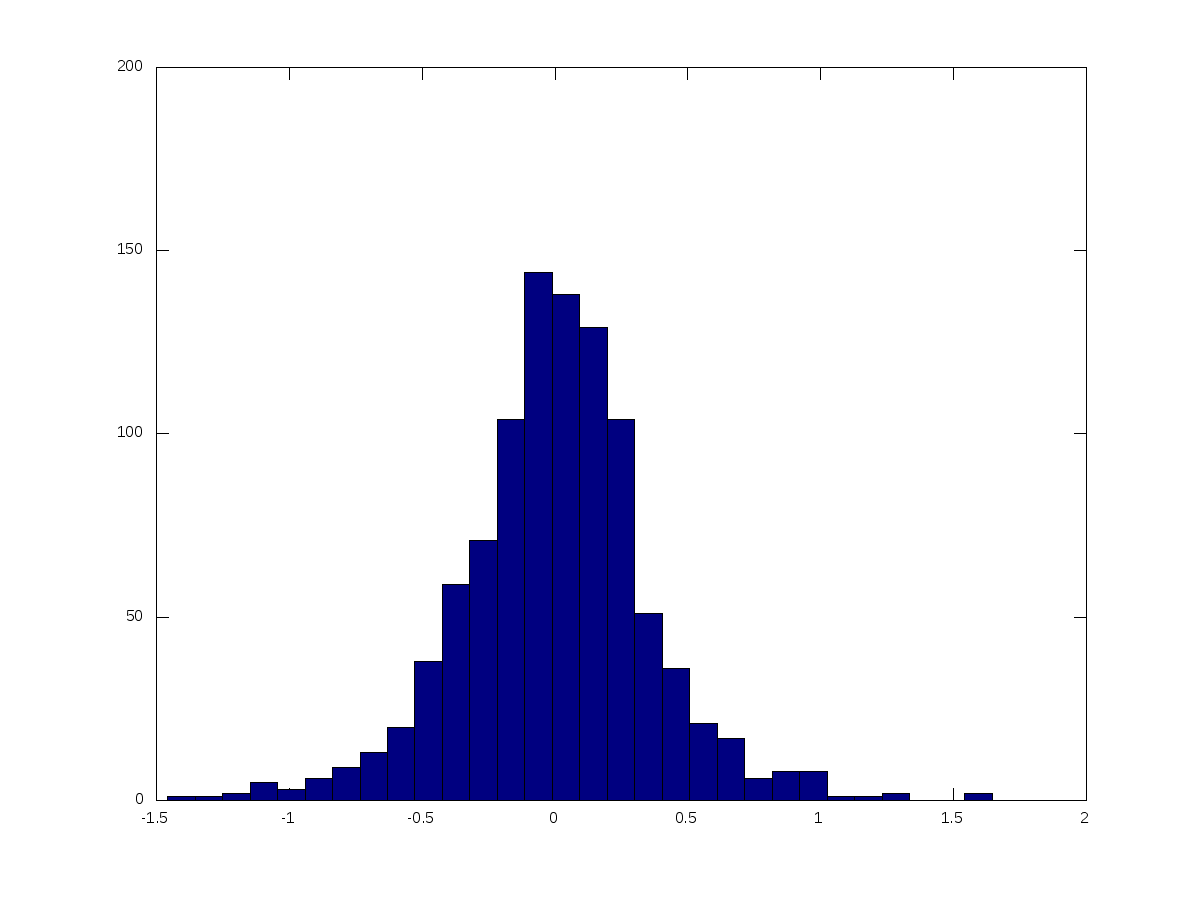
\includegraphics[width=10cm]{Examples/GLS/AR1ErrorsOLS}

}\subfloat[GLS]{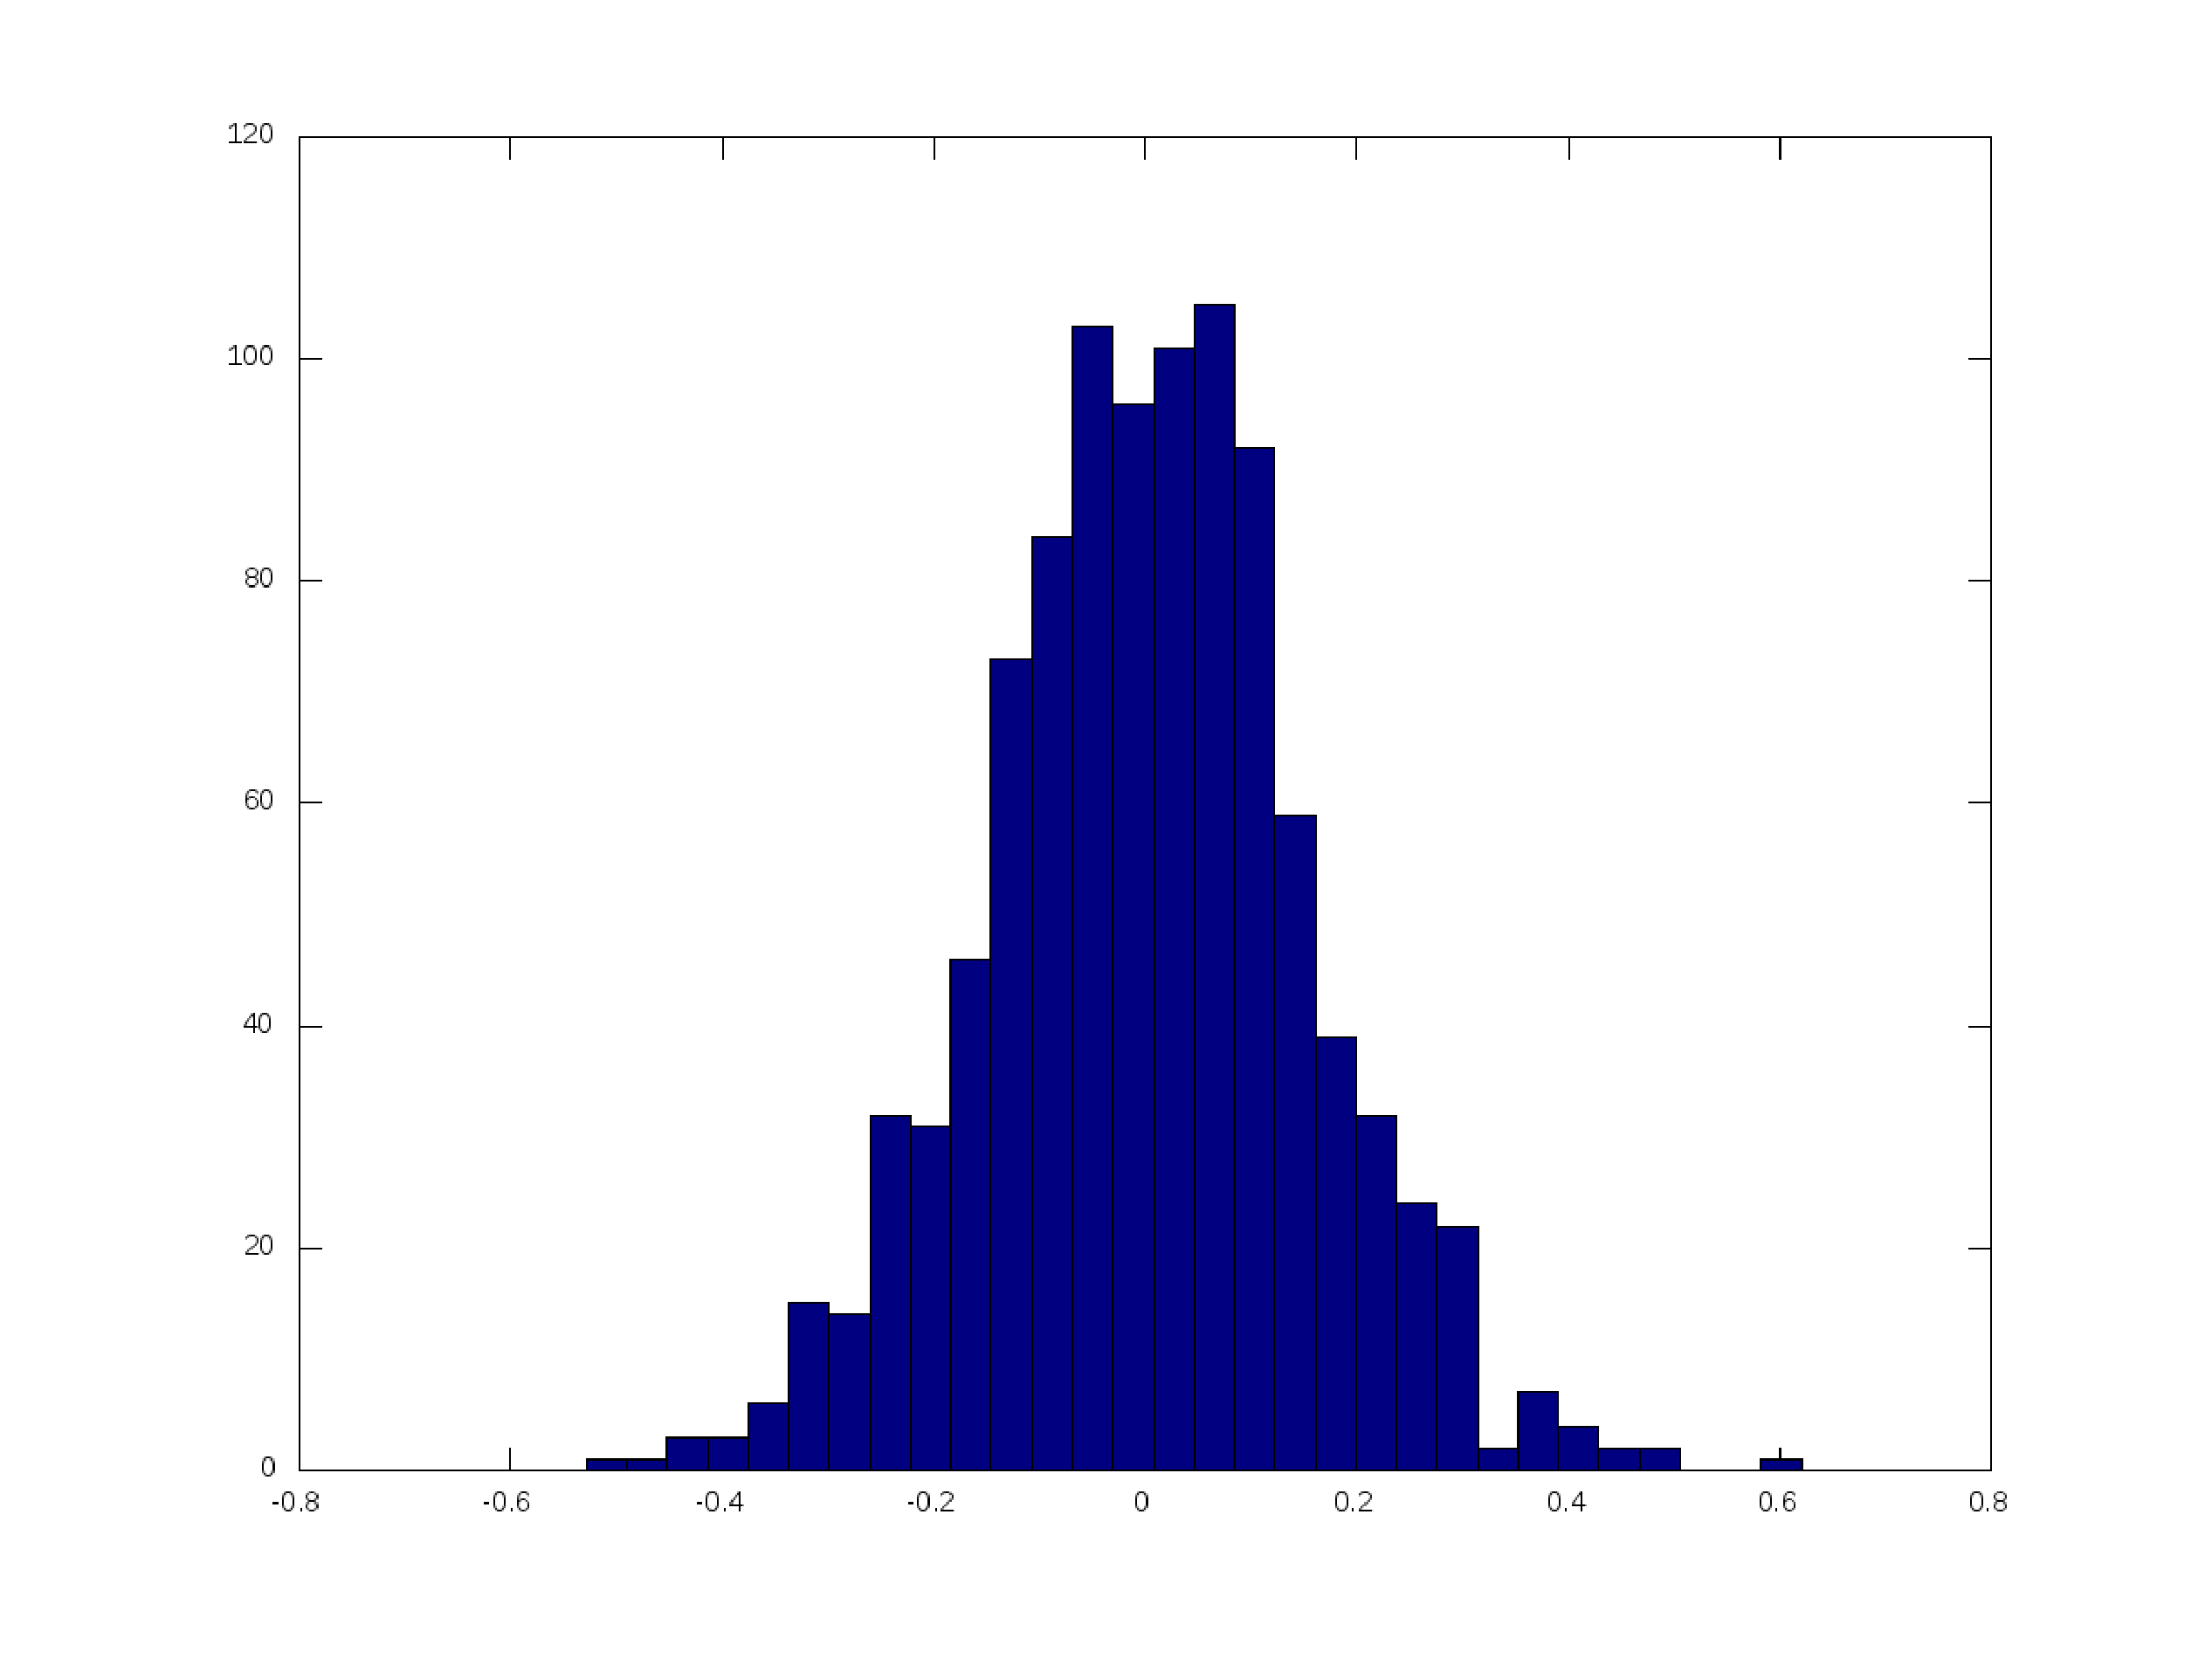
\includegraphics[width=10cm]{Examples/GLS/AR1ErrorsGLS}

}
\end{figure}



\subsection{\label{sub:Asymptotically-valid-inferences}Asymptotically valid inferences with autocorrelation of unknown form}

See Hamilton Ch. 10, pp. 261-2 and 280-84.

When the form of autocorrelation is unknown, one may decide to use the OLS estimator, without correction. We've seen that this estimator has the limiting distribution 
\[
\sqrt{n}\left(\hat{\beta}-\beta\right)\overset{d}{\rightarrow}N\left(0,Q_{X}^{-1}\Omega Q_{X}^{-1}\right)
\]
 where, as before, $\Omega$ is 
\[
\Omega=\lim_{n\rightarrow\infty}\mathcal{E}\left(\frac{X^{\prime}\varepsilon\varepsilon^{\prime}X}{n}\right)
\]
 We need a consistent estimate of $\Omega$. Define $m_{t}=x_{t}\varepsilon_{t}$ (recall that $x_{t}$ is defined as a $K\times1$ vector). Note that 
\begin{eqnarray*}
X^{\prime}\varepsilon & = & \left[\begin{array}{cccc}
x_{1} & x_{2} & \cdots & x_{n}\end{array}\right]\left[\begin{array}{c}
\varepsilon_{1}\\
\varepsilon_{2}\\
\vdots\\
\varepsilon_{n}
\end{array}\right]\\
 & = & \sum_{t=1}^{n}x_{t}\varepsilon_{t}\\
 & = & \sum_{t=1}^{n}m_{t}
\end{eqnarray*}
 so that 
\[
\Omega=\lim_{n\rightarrow\infty}\frac{1}{n}\mathcal{E}\left[\left(\sum_{t=1}^{n}m_{t}\right)\left(\sum_{t=1}^{n}m_{t}^{\prime}\right)\right]
\]
 We assume that $m_{t}$ is covariance stationary (so that the covariance between $m_{t}$ and $m_{t-s}$ does not depend on $t).$

Define the $v-th$ autocovariance of $m_{t}$ as 
\[
\Gamma_{v}=\mathcal{E}(m_{t}m_{t-v}^{\prime}).
\]
 Note that $\mathcal{E}(m_{t}m_{t+v}^{\prime})=\Gamma_{v}^{\prime}.$ \emph{(show this with an example).} In general, we expect that:
\begin{itemize}
\item $m_{t}$ will be autocorrelated, since $\varepsilon_{t}$ is potentially autocorrelated: 
\[
\Gamma_{v}=\mathcal{E}(m_{t}m_{t-v}^{\prime})\neq0
\]
 Note that this autocovariance does not depend on $t,$ due to covariance stationarity.
\item contemporaneously correlated ( $\mathcal{E}(m_{it}m_{jt})\neq0$ ), since the regressors in $x_{t}$ will in general be correlated (more on this later).
\item and heteroscedastic ($\mathcal{E}(m_{it}^{2})=\sigma_{i}^{2}$ , which depends upon $i$ ), again since the regressors will have different variances. 
\end{itemize}
While one could estimate $\Omega$ parametrically, we in general have little information upon which to base a parametric specification. Recent research has focused on consistent nonparametric estimators of $\Omega.$

Now define 
\[
\Omega_{n}=\mathcal{E}\frac{1}{n}\left[\left(\sum_{t=1}^{n}m_{t}\right)\left(\sum_{t=1}^{n}m_{t}^{\prime}\right)\right]
\]
 We have (\emph{show that the following is true, by expanding sum and shifting rows to left)}
\[
\Omega_{n}=\Gamma_{0}+\frac{n-1}{n}\left(\Gamma_{1}+\Gamma_{1}^{\prime}\right)+\frac{n-2}{n}\left(\Gamma_{2}+\Gamma_{2}^{\prime}\right)\cdots+\frac{1}{n}\left(\Gamma_{n-1}+\Gamma_{n-1}^{\prime}\right)
\]
 The natural, consistent estimator of $\Gamma_{v}$ is 
\[
\widehat{\Gamma_{v}}=\frac{1}{n}\sum_{t=v+1}^{n}\hat{m}_{t}\hat{m}_{t-v}^{\prime}.
\]
 where 
\[
\hat{m}_{t}=x_{t}\hat{\varepsilon}_{t}
\]
 (note: one could put $1/(n-v)$ instead of $1/n$ here). So, a natural, but inconsistent, estimator of $\Omega_{n}$ would be 
\begin{eqnarray*}
\hat{\Omega}_{n} & = & \widehat{\Gamma_{0}}+\frac{n-1}{n}\left(\widehat{\Gamma_{1}}+\widehat{\Gamma_{1}^{\prime}}\right)+\frac{n-2}{n}\left(\widehat{\Gamma_{2}}+\widehat{\Gamma_{2}^{\prime}}\right)+\cdots+\frac{1}{n}\left(\widehat{\Gamma_{n-1}}+\widehat{\Gamma_{n-1}^{\prime}}\right)\\
 & = & \widehat{\Gamma_{0}}+\sum_{v=1}^{n-1}\frac{n-v}{n}\left(\widehat{\Gamma_{v}}+\widehat{\Gamma_{v}^{\prime}}\right).
\end{eqnarray*}
 This estimator is inconsistent in general, since the number of parameters to estimate is more than the number of observations, and increases more rapidly than $n$, so information does not build up as $n\rightarrow\infty.$

On the other hand, supposing that $\Gamma_{v}$ tends to zero sufficiently rapidly as $v$ tends to $\infty,$ a modified estimator 
\[
\hat{\Omega}_{n}=\widehat{\Gamma_{0}}+\sum_{v=1}^{q(n)}\left(\widehat{\Gamma_{v}}+\widehat{\Gamma_{v}^{\prime}}\right),
\]
 where $q(n)\overset{p}{\rightarrow}\infty$ as $n\rightarrow\infty$ will be consistent, provided $q(n)$ grows sufficiently slowly.
\begin{itemize}
\item The assumption that autocorrelations die off is reasonable in many cases. For example, the AR(1) model with $|\rho|<1$ has autocorrelations that die off.
\item The term $\frac{n-v}{n}$ can be dropped because it tends to one for $v<q(n)$, given that $q(n)$ increases slowly relative to $n.$
\item A disadvantage of this estimator is that is may not be positive definite. This could cause one to calculate a negative $\chi^{2}$ statistic, for example!
\item Newey and West proposed and estimator (\emph{Econometrica}, 1987) that solves the problem of possible nonpositive definiteness of the above estimator. Their estimator is 
\[
\hat{\Omega}_{n}=\widehat{\Gamma_{0}}+\sum_{v=1}^{q(n)}\left[1-\frac{v}{q+1}\right]\left(\widehat{\Gamma_{v}}+\widehat{\Gamma_{v}^{\prime}}\right).
\]
 This estimator is p.d. by construction. The condition for consistency is that $n^{-1/4}q(n)\rightarrow0.$ Note that this is a very slow rate of growth for $q.$ This estimator is nonparametric - we've placed no parametric restrictions on the form of $\Omega.$ It is an example of a \emph{kernel} estimator. 
\end{itemize}
Finally, since $\Omega_{n}$ has $\Omega$ as its limit, $\hat{\Omega}_{n}\overset{p}{\rightarrow}\Omega.$ We can now use $\hat{\Omega}_{n}$ and $\widehat{Q_{X}}=\frac{1}{n}X^{\prime}X$ to consistently estimate the limiting distribution of the OLS\ estimator under heteroscedasticity and autocorrelation of unknown form. With this, asymptotically valid tests are constructed in the usual way.


\subsection{Testing for autocorrelation}

\textbf{Durbin-Watson test}

The Durbin-Watson test is not strictly valid in most situations where we would like to use it. Nevertheless, it is encountered often enough so that one should know something about it. The Durbin-Watson test statistic is 
\begin{eqnarray*}
DW & = & \frac{\sum_{t=2}^{n}\left(\hat{\varepsilon}_{t}-\hat{\varepsilon}_{t-1}\right)^{2}}{\sum_{t=1}^{n}\hat{\varepsilon}_{t}^{2}}\\
 & = & \frac{\sum_{t=2}^{n}\left(\hat{\varepsilon}_{t}^{2}-2\hat{\varepsilon}_{t}\hat{\varepsilon}_{t-1}+\hat{\varepsilon}_{t-1}^{2}\right)}{\sum_{t=1}^{n}\hat{\varepsilon}_{t}^{2}}
\end{eqnarray*}

\begin{itemize}
\item The null hypothesis is that the first order autocorrelation of the errors is zero: $H_{0}:\rho_{1}=0.$ The alternative is of course $H_{A}:\rho_{1}\neq0.$ Note that the alternative is not that the errors are AR(1), since many general patterns of autocorrelation will have the first order autocorrelation different than zero. For this reason the test is useful for detecting autocorrelation in general. For the same reason, one shouldn't just assume that an AR(1) model is appropriate when the DW test rejects the null.
\item Under the null, the middle term tends to zero, and the other two tend to one, so $DW\overset{p}{\rightarrow}2.$
\item Supposing that we had an AR(1) error process with $\rho=1.$ In this case the middle term tends to $-2,$ so $DW\overset{p}{\rightarrow}0$
\item Supposing that we had an AR(1) error process with $\rho=-1.$ In this case the middle term tends to $2,$ so $DW\overset{p}{\rightarrow}4$
\item These are the extremes: $DW$ always lies between 0 and 4.
\item The distribution of the test statistic depends on the matrix of regressors, $X,$ so tables can't give exact critical values. The give upper and lower bounds, which correspond to the extremes that are possible. See Figure \ref{fig:Durbin-Watson-critical-values}. There are means of determining exact critical values conditional on $X.$
\item Note that DW\ can be used to test for nonlinearity (add discussion). 
\item The DW test is based upon the assumption that the matrix $X$ is fixed in repeated samples. This is often unreasonable in the context of economic time series, which is precisely the context where the test would have application. It is possible to relate the DW test to other test statistics which are valid without strict exogeneity.
\end{itemize}
\begin{figure}
\caption{\label{fig:Durbin-Watson-critical-values}Durbin-Watson critical values}
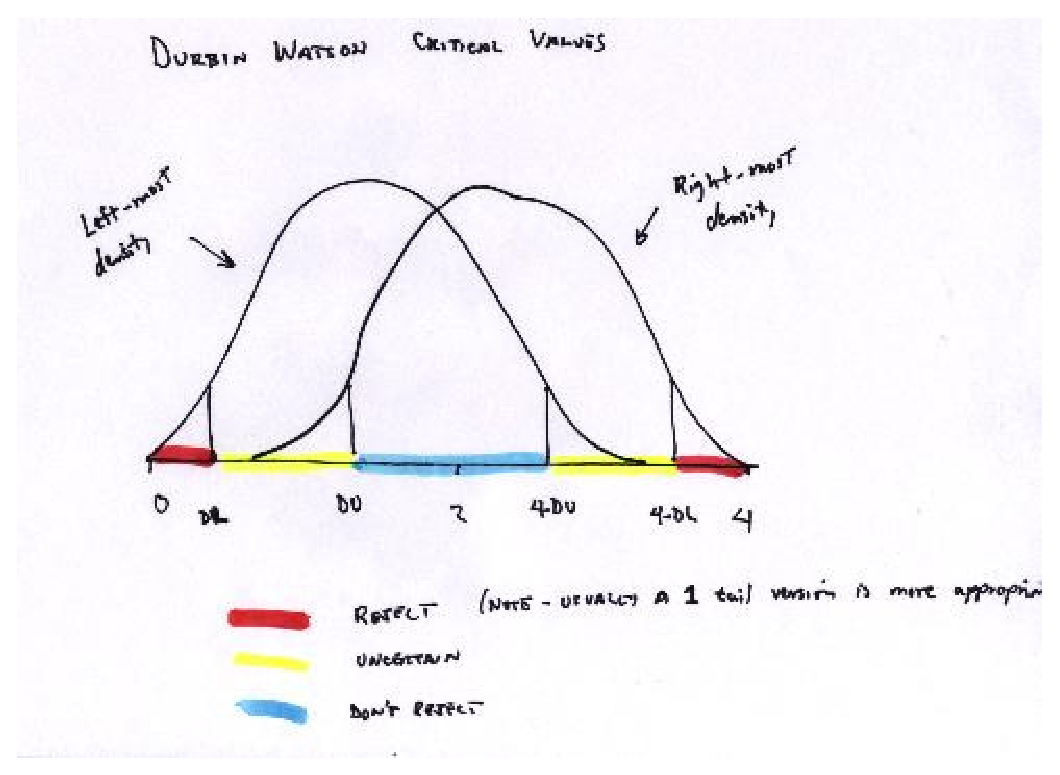
\includegraphics[width=15cm]{Examples/Figures/DurbinWatson}
\end{figure}


\textbf{Breusch-Godfrey test}

This test uses an auxiliary regression, as does the White test for heteroscedasticity. The regression is 
\[
\hat{\varepsilon}_{t}=x_{t}^{\prime}\delta+\gamma_{1}\hat{\varepsilon}_{t-1}+\gamma_{2}\hat{\varepsilon}_{t-2}+\cdots+\gamma_{P}\hat{\varepsilon}_{t-P}+v_{t}
\]
 and the test statistic is the $nR^{2}$ statistic, just as in the White test. There are $P$ restrictions, so the test statistic is asymptotically distributed as a $\chi^{2}(P).$
\begin{itemize}
\item The intuition is that the lagged errors shouldn't contribute to explaining the current error if there is no autocorrelation.
\item $x_{t}$ is included as a regressor to account for the fact that the $\hat{\varepsilon}_{t}$ are not independent even if the $\varepsilon_{t}$ are. This is a technicality that we won't go into here.
\item This test is valid even if the regressors are stochastic and contain lagged dependent variables, so it is considerably more useful than the DW test for typical time series data.
\item The alternative is not that the model is an AR(P), following the argument above. The alternative is simply that some or all of the first $P\;$autocorrelations are different from zero. This is compatible with many specific forms of autocorrelation. 
\end{itemize}

\subsection{Lagged dependent variables and autocorrelation}

We've seen that the OLS\ estimator is consistent under autocorrelation, as long as $plim\frac{X^{\prime}\varepsilon}{n}=0.$ This will be the case when $\mathcal{E}(X^{\prime}\varepsilon)$ $=0,$ following a LLN. An important exception is the case where $X$ contains lagged $y^{\prime}s$ and the errors are autocorrelated.
\begin{example}
\label{exa:-Dynamic-model}Dynamic model with MA1 errors. Consider the model 
\begin{eqnarray*}
y_{t} & = & \alpha+\rho y_{t-1}+\beta x_{t}+\epsilon_{t}\\
\epsilon_{t} & = & \upsilon_{t}+\phi\upsilon_{t-1}
\end{eqnarray*}
We can easily see that a regressor is not weakly exogenous: 
\begin{eqnarray*}
\mathcal{E}(y_{t-1}\varepsilon_{t}) & = & \mathcal{E}\left\{ (\alpha+\rho y_{t-2}+\beta x_{t-1}+\upsilon_{t-1}+\phi\upsilon_{t-2})(\upsilon_{t}+\phi\upsilon_{t-1})\right\} \\
 & \neq & 0
\end{eqnarray*}
 since one of the terms is $\mathcal{E}(\phi\upsilon_{t-1}^{2})$ which is clearly nonzero. In this case $\mathcal{E}(\mathbf{x}_{t}\varepsilon_{t})\neq0,$ and therefore $plim\frac{X^{\prime}\varepsilon}{n}\neq0.$ Since

\[
plim\hat{\beta}=\beta+plim\frac{X^{\prime}\varepsilon}{n}
\]
 the OLS\ estimator is inconsistent in this case. One needs to estimate by instrumental variables (IV), which we'll get to later
\end{example}
The Octave script  \htmladdnormallink{GLS/DynamicMA.m}{file:///home/michael/Mystuff/Econometrics/Examples/GLS/DynamicMA.m}  does a Monte Carlo study. The sample size is $n=100$. The true coefficients are $\alpha=1$ $\rho=0.9$ and $\beta=1$. The MA parameter is $\phi=-0.95$. Figure \ref{fig:Dynamic-model-with} gives the results. You can see that the constant and the autoregressive parameter have a lot of bias. By re-running the script with $\phi=0$, you will see that much of the bias disappears (not all - why?).\newpage{}
\begin{figure}
\caption{\label{fig:Dynamic-model-with}Dynamic model with MA(1) errors}


\subfloat[$\hat{\alpha}-\alpha$]{

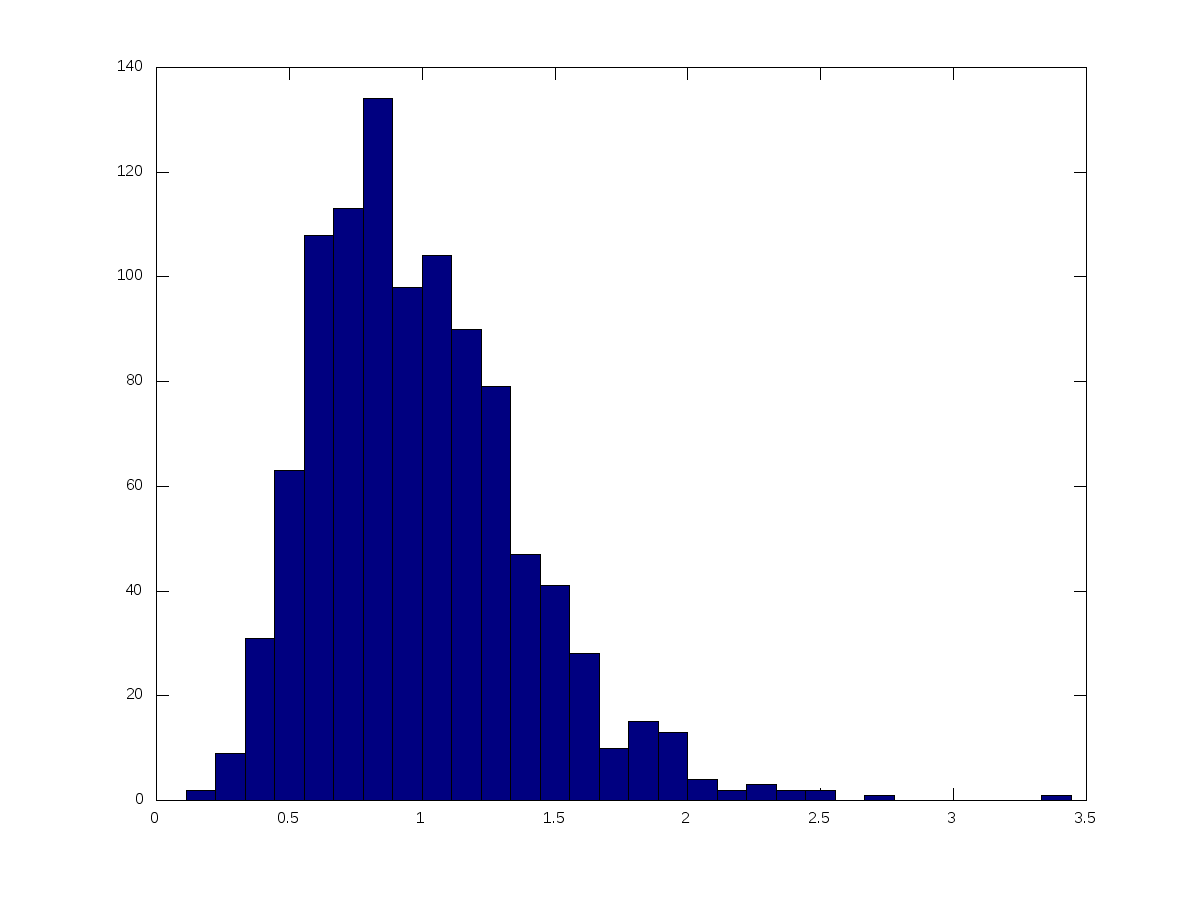
\includegraphics[width=10cm]{Examples/GLS/constant_n100}}

\subfloat[$\hat{\rho}-\rho$]{

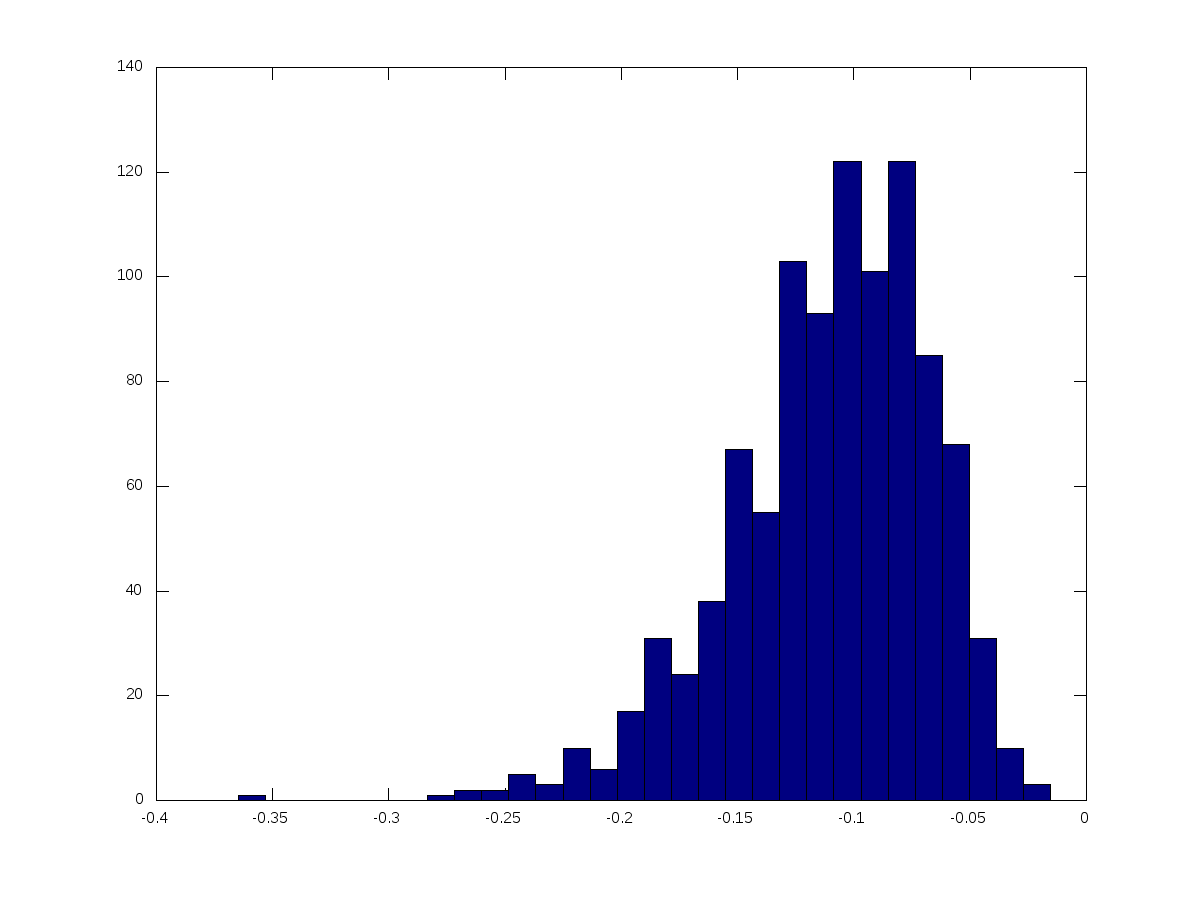
\includegraphics[width=10cm]{Examples/GLS/ylag_n100}}

\subfloat[$\hat{\beta}-\beta$]{

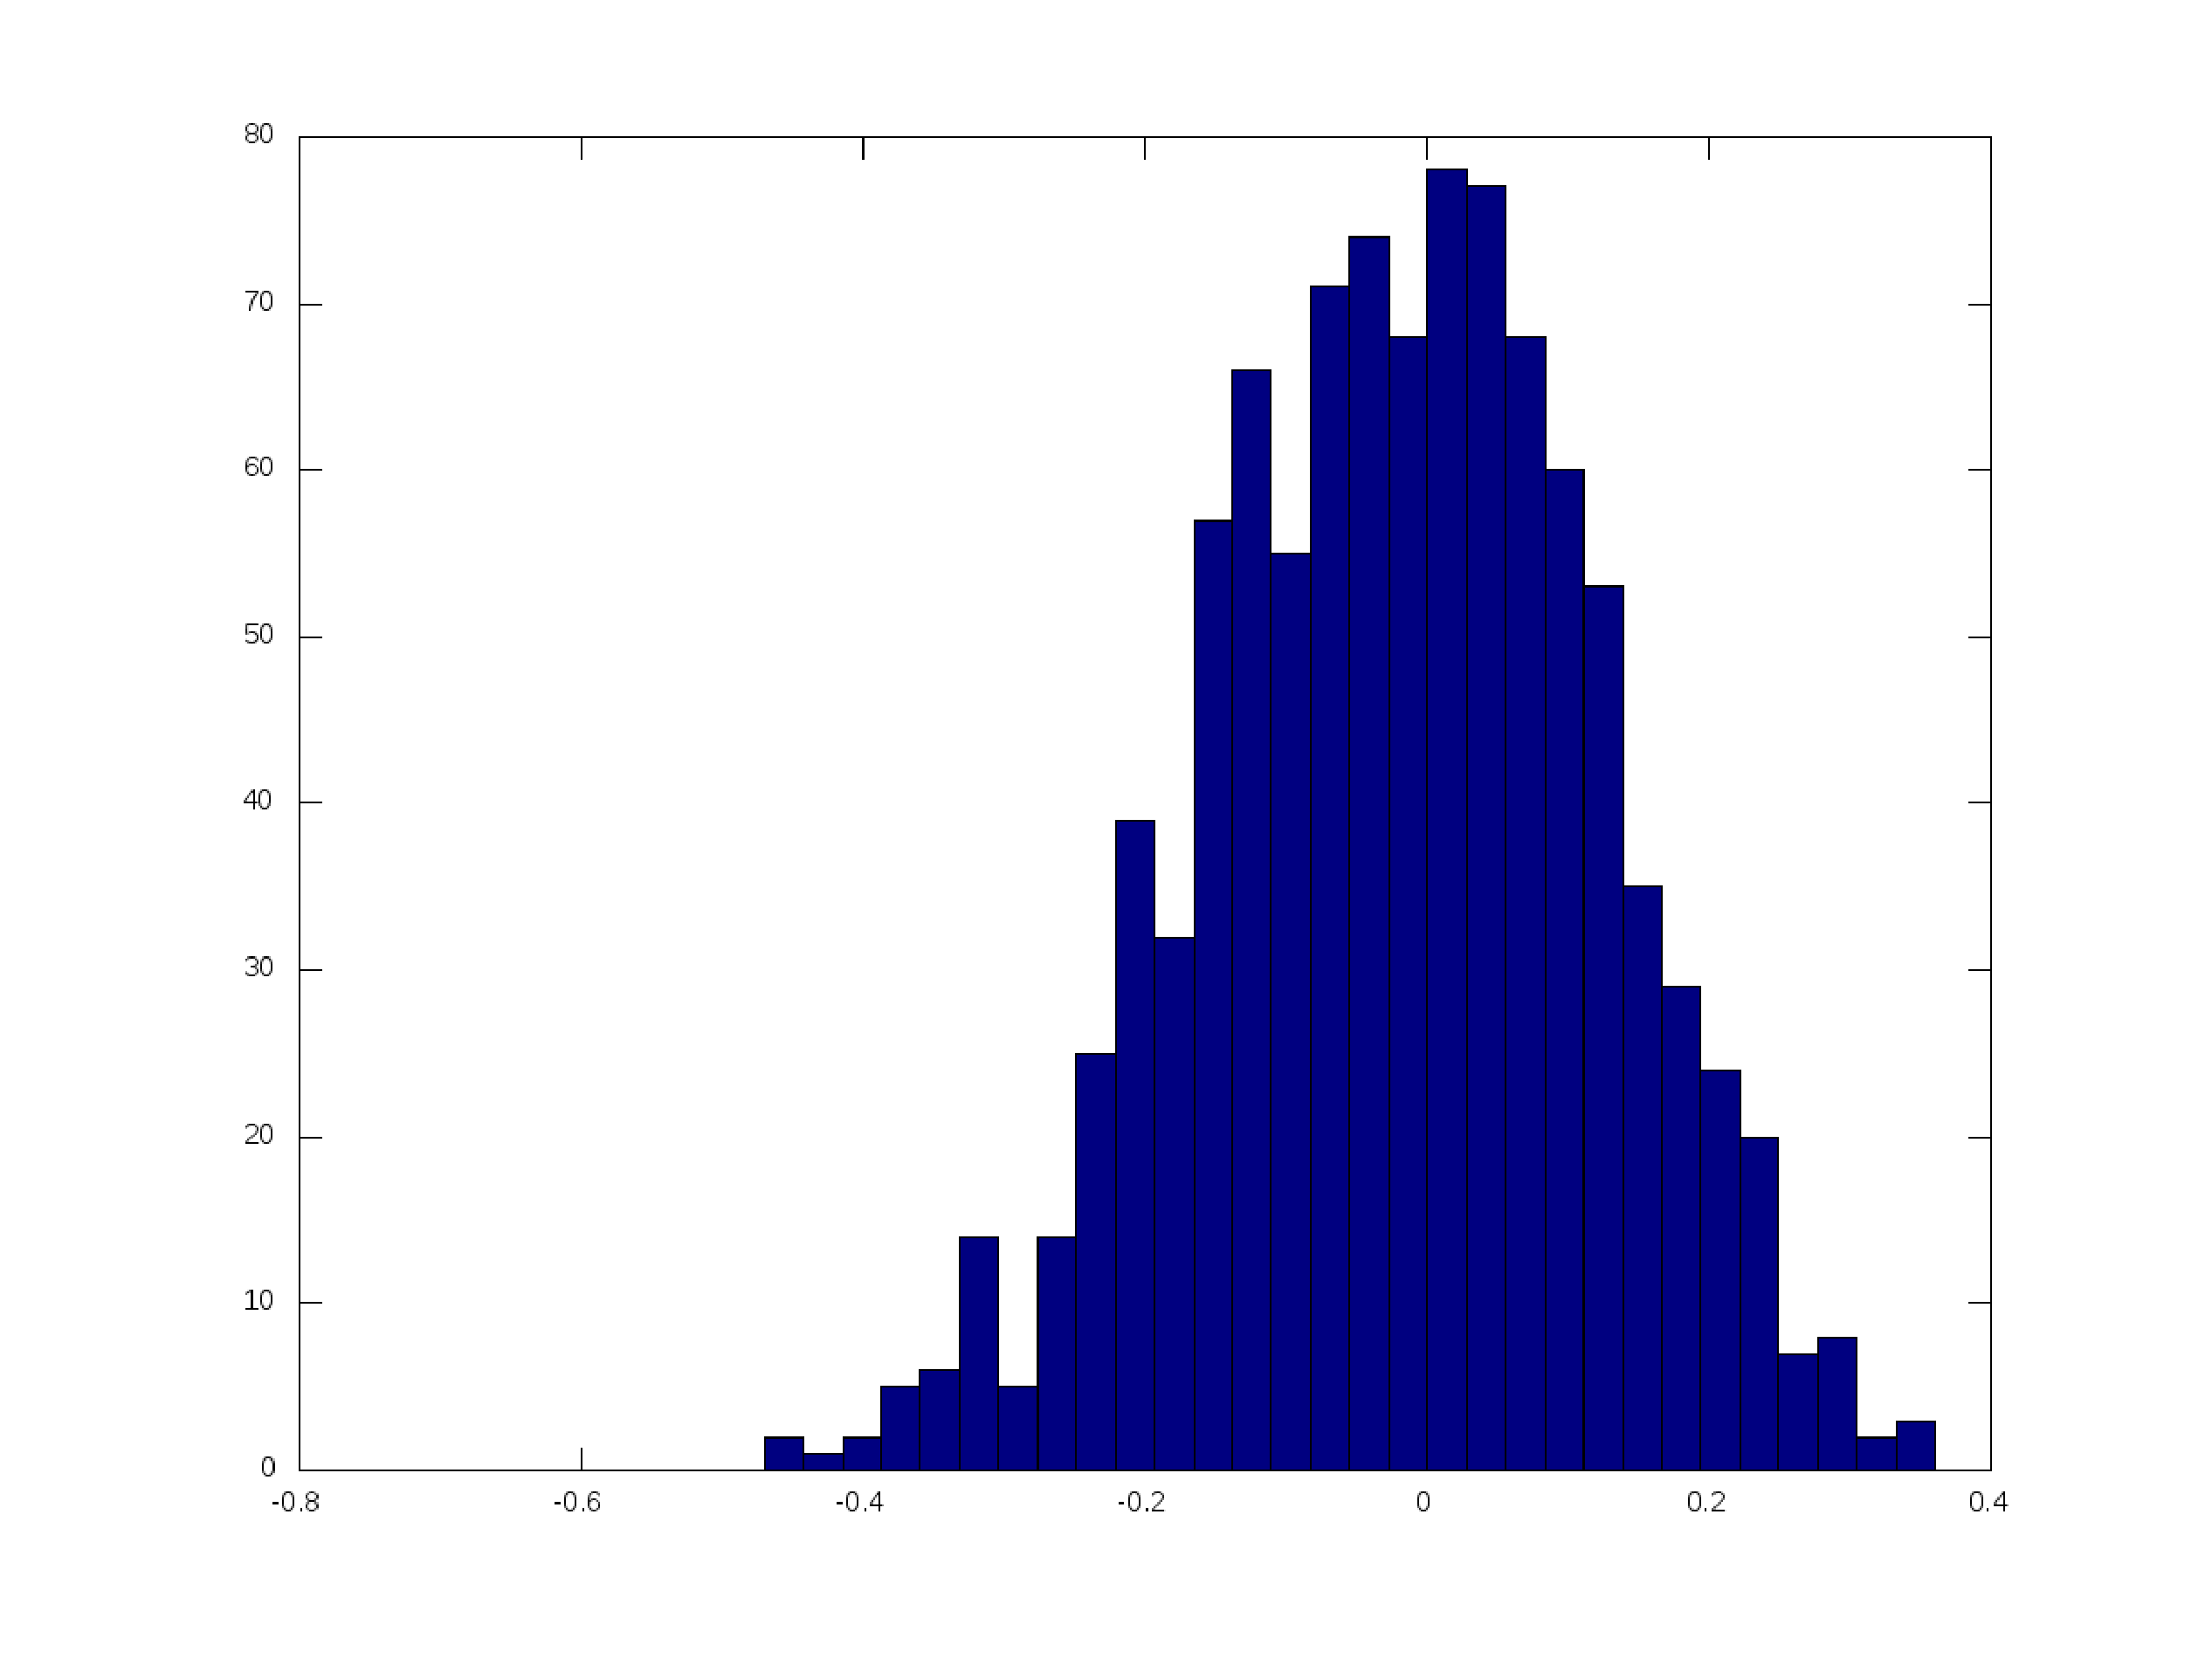
\includegraphics[width=10cm]{Examples/GLS/x_n100}}
\end{figure}


\newpage{}


\subsection{Examples}


\paragraph{Nerlove model, yet again}

The Nerlove model uses cross-sectional data, so one may not think of performing tests for autocorrelation. However, specification error can induce autocorrelated errors. Consider the simple Nerlove model 
\[
\ln C=\beta_{1}+\beta_{2}\ln Q+\beta_{3}\ln P_{L}+\beta_{4}\ln P_{F}+\beta_{5}\ln P_{K}+\epsilon
\]
 and the extended Nerlove model 
\[
\ln C=\sum_{j=1}^{5}\alpha_{j}D_{j}+\sum_{j=1}^{5}\gamma_{j}D_{j}\ln Q+\beta_{L}\ln P_{L}+\beta_{F}\ln P_{F}+\beta_{K}\ln P_{K}+\epsilon
\]
discussed around equation \ref{Nerlove, favorite model}. If you have done the exercises, you have seen evidence that the extended model is preferred. So if it is in fact the proper model, the simple model is misspecified. Let's check if this misspecification might induce autocorrelated errors.

The Octave program  \htmladdnormallink{GLS/NerloveAR.m}{file:///home/michael/Mystuff/Econometrics/Examples/GLS/NerloveAR.m} estimates the simple Nerlove model, and plots the residuals as a function of $\ln Q$, and it calculates a Breusch-Godfrey test statistic. The residual plot is in Figure \ref{Nerlove - misspec induces autocorrelation} , and the test results are: \verbatiminput{Examples/GLS/BGTest.out}Clearly, there is a problem of autocorrelated residuals.

Repeat the autocorrelation tests using the extended Nerlove model (Equation \ref{Nerlove, favorite model}) to see the problem is solved.

\begin{figure}
\caption{\label{Nerlove - misspec induces autocorrelation}Residuals of simple Nerlove model}


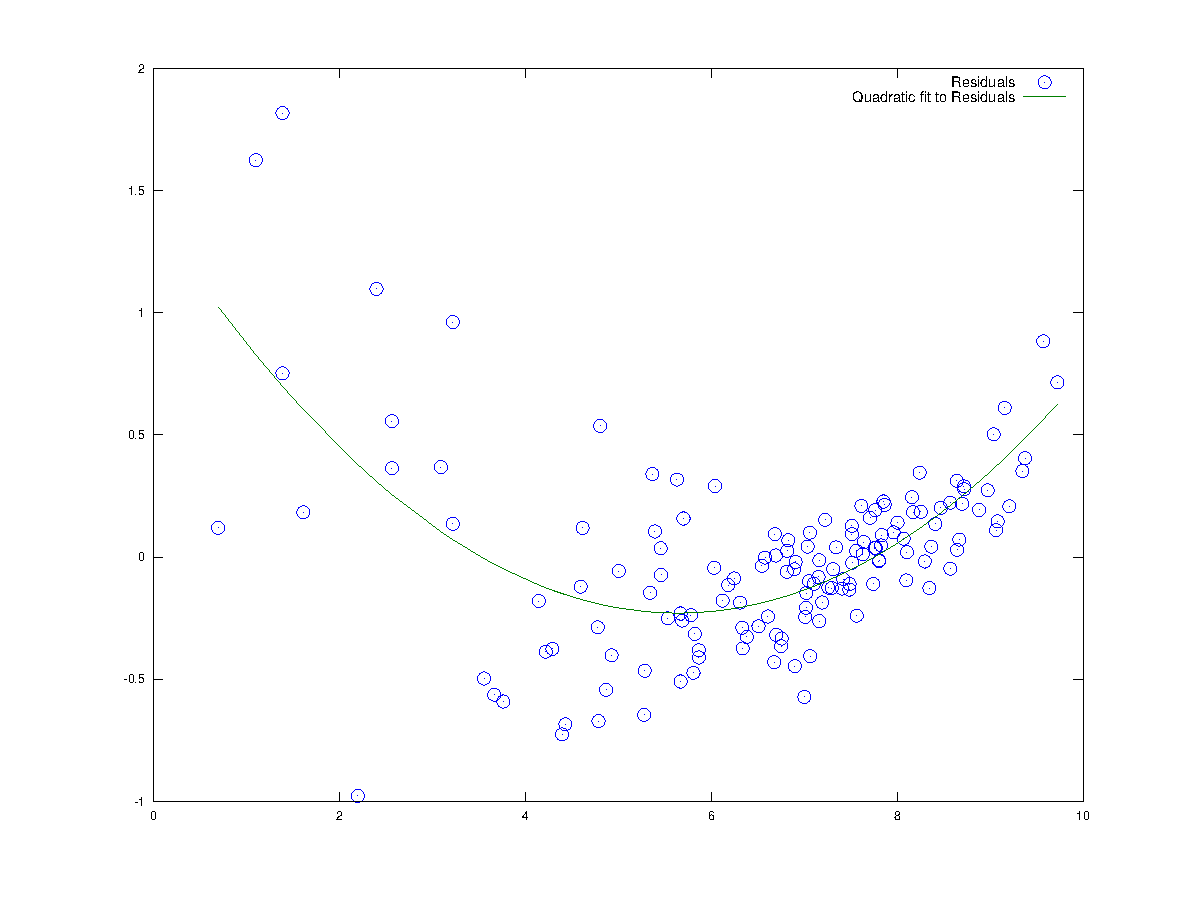
\includegraphics{Examples/GLS/NerloveAR}
\end{figure}



\paragraph{Klein model}

Klein's Model I is a simple macroeconometric model. One of the equations in the model explains consumption ($C$) as a function of profits ($P$), both current and lagged, as well as the sum of wages in the private sector ($W^{p}$) and wages in the government sector ($W^{g}$). Have a look at the \htmladdnormallink{README}{file:///home/michael/Mystuff/Econometrics/Examples/Data/klein_readme.txt}  file for this data set. This gives the variable names and other information.

Consider the model
\[
C_{t}=\alpha_{0}+\alpha_{1}P_{t}+\alpha_{2}P_{t-1}+\alpha_{3}(W_{t}^{p}+W_{t}^{g})+\epsilon_{1t}
\]
The Octave program  \htmladdnormallink{GLS/Klein.m}{file:///home/michael/Mystuff/Econometrics/Examples/GLS/Klein.m} estimates this model by OLS, plots the residuals, and performs the Breusch-Godfrey test, using 1 lag of the residuals. The estimation and test results are:\verbatiminput{Examples/GLS/Klein.out} and the residual plot is in Figure \ref{cap:OLS-residuals,-Klein}. The test does not reject the null of nonautocorrelatetd errors, but we should remember that we have only 21 observations, so power is likely to be fairly low. The residual plot leads me to suspect that there may be autocorrelation - there are some significant runs below and above the x-axis. Your opinion may differ. 
\begin{figure}
\caption{\label{cap:OLS-residuals,-Klein}OLS residuals, Klein consumption equation}


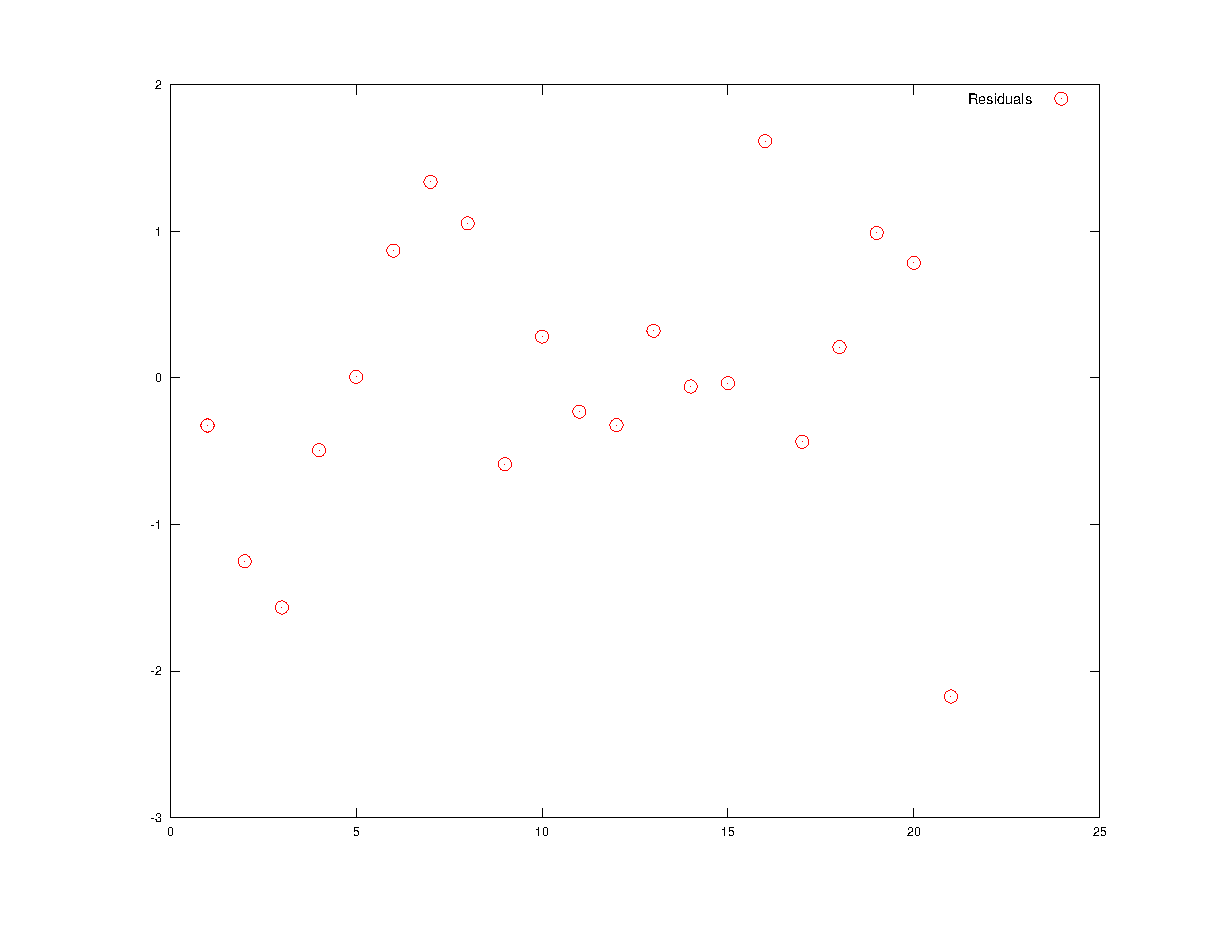
\includegraphics{Examples/GLS/KleinResiduals}
\end{figure}


Since it seems that there \emph{may} be autocorrelation, lets's try an AR(1) correction. The Octave program  \htmladdnormallink{GLS/KleinAR1.m}{file:///home/michael/Mystuff/Econometrics/Examples/GLS/KleinAR1.m} estimates the Klein consumption equation assuming that the errors follow the AR(1) pattern. The results, with the Breusch-Godfrey test for remaining autocorrelation are: \verbatiminput{Examples/GLS/KleinAR1.out}
\begin{itemize}
\item The test is farther away from the rejection region than before, and the residual plot is a bit more favorable for the hypothesis of nonautocorrelated residuals, IMHO. For this reason, it seems that the AR(1) correction might have improved the estimation.
\item Nevertheless, there has not been much of an effect on the estimated coefficients nor on their estimated standard errors. This is probably because the estimated AR(1) coefficient is not very large (around 0.2)
\item The existence or not of autocorrelation in this model will be important later, in the section on simultaneous equations.
\end{itemize}

\section{Exercises}
\begin{enumerate}
\item Comparing the variances of the OLS and GLS estimators, I claimed that the following holds:
\begin{eqnarray*}
Var(\hat{\beta})-Var(\hat{\beta}_{GLS}) & = & A\Sigma A^{'}
\end{eqnarray*}
Verify that this is true.
\item Show that the GLS estimator can be defined as
\[
\hat{\beta}_{GLS}=\arg\min(y-X\beta)^{\prime}\Sigma^{-1}(y-X\beta)
\]

\item The limiting distribution of the OLS estimator with heteroscedasticity of unknown form is
\[
\sqrt{n}\left(\hat{\beta}-\beta\right)\overset{d}{\rightarrow}N\left(0,Q_{X}^{-1}\Omega Q_{X}^{-1}\right),
\]
 where
\[
\lim_{n\rightarrow\infty}\mathcal{E}\left(\frac{X^{\prime}\varepsilon\varepsilon^{\prime}X}{n}\right)=\Omega
\]
 Explain why
\[
\widehat{\Omega}=\frac{1}{n}\sum_{t=1}^{n}x_{t}x_{t}^{\prime}\hat{\varepsilon}_{t}^{2}
\]
 is a consistent estimator of this matrix.
\item Define the $v-th$ autocovariance of a covariance stationary process $m_{t}$, where $E(m_{t})=0$ as 
\[
\Gamma_{v}=\mathcal{E}(m_{t}m_{t-v}^{\prime}).
\]
 Show that $\mathcal{E}(m_{t}m_{t+v}^{\prime})=\Gamma_{v}^{\prime}.$
\item For the Nerlove model with dummies and interactions discussed above (see Section \ref{sub:Nerlove GLS by groups} and equation \ref{Nerlove, favorite model}) 
\[
\ln C=\sum_{j=1}^{5}\alpha_{j}D_{j}+\sum_{j=1}^{5}\gamma_{j}D_{j}\ln Q+\beta_{L}\ln P_{L}+\beta_{F}\ln P_{F}+\beta_{K}\ln P_{K}+\epsilon
\]
above, we did a GLS correction based on the assumption that there is HET by groups ($V(\epsilon_{t}|x_{t})=\sigma_{j}^{2}$). Let's assume that this model is correctly specified, except that there may or may not be HET, and if it is present it may be of the form assumed, or perhaps of some other form. What happens if the assumed form of HET is incorrect?

\begin{enumerate}
\item Is the ''FGLS'' based on the assumed form of HET consistent?
\item Is it efficient? Is it likely to be efficient with respect to OLS?
\item Are hypothesis tests using the ''FGLS'' estimator valid? If not, can they be made valid following some procedure? Explain.
\item Are the t-statistics reported in Section \ref{sub:Nerlove GLS by groups} valid?
\item Which estimator do you prefer, the OLS estimator or the FGLS estimator? Discuss.
\end{enumerate}
\item Perhaps we can be a little more parsimonious with the Nerlove data (\htmladdnormallink{nerlove.data}{file:///home/michael/Mystuff/Econometrics/Examples/Data/nerlove.data} ), rather than using so many parameters to account for non-constant returns to scale, and to account for heteroscedasticity. Consider the original model 
\[
\ln C=\beta+\beta_{Q}\ln Q+\beta_{L}\ln P_{L}+\beta_{F}\ln P_{F}+\beta_{K}\ln P_{K}+\epsilon
\]


\begin{enumerate}
\item Estimate by OLS, plot the residuals, and test for autocorrelation and heteroscedasticity. Explain your findings.
\item Consider the model
\[
\ln C=\beta+\beta_{Q}\ln Q+\gamma_{Q}\left(\ln Q\right)^{2}+\beta_{L}\ln P_{L}+\beta_{F}\ln P_{F}+\beta_{K}\ln P_{K}+\epsilon
\]


\begin{enumerate}
\item Explain how this model can account for non-constant returns to scale. 
\item estimate this model, and test for autocorrelation and heteroscedasticity. You should find that there is HET, but no strong evidence of AUT. Why is this the case?
\item Do a GLS correction where it is assumed that $V(\epsilon_{i})=\frac{\sigma^{2}}{\left(\ln Q_{i}\right)^{2}}$. In GRETL, there is a weighted least squares option that you can use. Why does this assumed form of HET make sense?
\item plot the weighted residuals versus output. Is there evidence of HET, or has the correction eliminated the problem?
\item plot the fitted values for returns to scale, for all of the firms.
\end{enumerate}
\end{enumerate}
\item The \htmladdnormallink{hall.csv}{file:///home/michael/Mystuff/Econometrics/Examples/Data/hall.csv}  or \htmladdnormallink{hall.gdt}{file:///home/michael/Mystuff/Econometrics/Examples/Data/hall.gdt}  dataset contains monthly observation on 3 variables: the consumption ratio $c_{t}/c_{t-1}$; the gross return of an equally weighted index of assets $ewr_{t}$; and the gross return of the same index, but weighted by value, $vwr_{t}$. The idea is that a representative consumer may finance consumption by investing in assets. Present wealth is used for two things: consumption and investment. The return on investment defines wealth in the next period, and the process repeats. For the moment, explore the properties of the variables.

\begin{enumerate}
\item Are the variances constant over time?
\item Do the variables appear to be autocorrelated? Hint: regress a variable on its own lags.
\item Do the variable seem to be normally distributed?
\item Look at the properties of the growth rates of the variables: repeat a-c for growth rates. The growth rate of a variable $x_{t}$ is given by $\log\left(x_{t}/x_{t-1}\right)$.
\end{enumerate}
\item Consider the model
\begin{align*}
y_{t} & =C+A_{1}y_{t-1}+\epsilon_{t}\\
E(\epsilon_{t}\epsilon_{t}^{\prime}) & =\Sigma\\
E(\epsilon_{t}\epsilon_{s}^{\prime}) & =0,t\ne s
\end{align*}
where $y_{t}$ and $\epsilon_{t}$ are $G\times1$ vectors, $C$ is a $G\times1$ of constants, and $A_{1}$is a $G\times G$ matrix of parameters. The matrix $\Sigma$ is a $G\times G$ covariance matrix. Assume that we have $n$ observations. This is a \emph{vector autoregressive} model, of order 1 - commonly referred to as a VAR(1) model.

\begin{enumerate}
\item Show how the model can be written in the form $Y=X\beta+\nu$, where $Y$ is a $Gn\times1$ vector, $\beta$ is a $(G+G^{2})\times$1 parameter vector, and the other items are conformable. What is the structure of $X$? What is the structure of the covariance matrix of $\nu$?
\item This model has HET and AUT. Verify this statement.
\item Set $G=2,$$C=(0\,0)^{\prime}$$A=\left[\begin{array}{cc}
0.8 & -0.1\\
0.2 & 0.5
\end{array}\right]$, $\Sigma=\left[\begin{array}{cc}
1 & 0.5\\
0.5 & 1
\end{array}\right]$. Simulate data from this model, then estimate the model using OLS and feasible GLS. You should find that the two estimators are identical, which might seem surprising, given that there is HET and AUT.
\item \label{enu:(advanced).-Prove-analytically}(optional, and advanced). Prove analytically that the OLS and GLS estimators are identical. Hint: this model is of the form of \emph{seemingly unrelated regressions}. 
\end{enumerate}
\item Consider the model
\begin{align*}
y_{t} & =\alpha+\rho_{1}y_{t-1}+\rho_{2}y_{t-2}+\epsilon_{t}
\end{align*}
where $\epsilon_{t}$ is a $N(0,1)$ white noise error. This is an autogressive model of order 2 (AR2) model. Suppose that data is generated from the AR2 model, but the econometrician mistakenly decides to estimate an AR1 model ($y_{t}=\alpha+\rho_{1}y_{t-1}+\epsilon_{t}$).

\begin{enumerate}
\item simulate data from the AR2 model, setting $\rho_{1}=0.5$ and $\rho_{2}=0.4,$ using a sample size of $n=30.$ 
\item Estimate the AR1 model by OLS, using the simulated data
\item test the hypothesis that $\rho_{1}=0.5$
\item test for autocorrelation using the test of your choice
\item repeat the above steps 10000 times.

\begin{enumerate}
\item What percentage of the time does a t-test reject the hypothesis that $\rho_{1}=0.5$?
\item What percentage of the time is the hypothesis of no autocorrelation rejected?
\end{enumerate}
\item discuss your findings. Include a residual plot for a representative sample.
\end{enumerate}
\item Modify the script given in Subsection \ref{sub:Monte-Carlo-example:} so that the first observation is dropped, rather than given special treatment. This corresponds to using the Cochrane-Orcutt method, whereas the script as provided implements the Prais-Winsten method. Check if there is an efficiency loss when the first observation is dropped.
\end{enumerate}
\newpage{}


\chapter{Endogeneity and simultaneity}

Several times we've encountered cases where correlation between regressors and the error term lead to biasedness and inconsistency of the OLS estimator. Cases include autocorrelation with lagged dependent variables (Example \ref{exa:-Dynamic-model}), measurement error in the regressors (Example \ref{exa:Measurement-error-in}) and missing regressors (Section \ref{sec:Missing-regressors}). Another important case we have not seen yet is that of simultaneous equations. The cause is different, but the effect is the same: bias and inconsistency when OLS is applied to a single equation. The basic idea is presented in Figure \ref{fig:Exogeneity-and-Endogeneity}. A simple regression will estimate the overall effect of x on y. If we're interested in the direct effect, $\beta$, then we have a problem when the overall effect and the direct effect differ.

\begin{figure}


\caption{\label{fig:Exogeneity-and-Endogeneity}Exogeneity and Endogeneity (adapted from Cameron and Trivedi)}


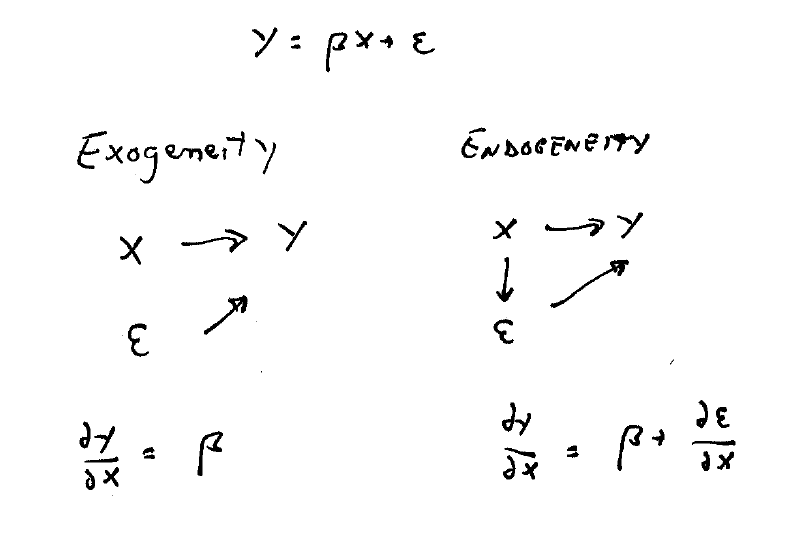
\includegraphics[width=12cm]{Examples/Figures/EndogExog}

\end{figure}



\section{Simultaneous equations}

Up until now our model is 
\[
y=X\beta+\varepsilon
\]
where we assume weak exogeneity of the regressors, so that $E(x_{t}\epsilon_{t})=0$. With weak exogeneity, the OLS estimator has desirable large sample properties (consistency, asymptotic normality).

Simultaneous equations is a different prospect. An example of a simultaneous equation system is a simple supply-demand system: 
\begin{eqnarray}
\text{Demand:\;\ }q_{t} & = & \alpha_{1}+\alpha_{2}p_{t}+\alpha_{3}y_{t}+\varepsilon_{1t}\label{eq:demand function}\\
\text{Supply:\;\ }q_{t} & = & \beta_{1}+\beta_{2}p_{t}+\varepsilon_{2t}\nonumber \\
\mathcal{E}\left(\left[\begin{array}{l}
\varepsilon_{1t}\\
\varepsilon_{2t}
\end{array}\right]\left[\begin{array}{ll}
\varepsilon_{1t} & \varepsilon_{2t}\end{array}\right]\right) & = & \left[\begin{array}{ll}
\sigma_{11} & \sigma_{12}\\
\cdot & \sigma_{22}
\end{array}\right]\nonumber \\
 & \equiv & \Sigma,\forall t\nonumber 
\end{eqnarray}
 The presumption is that $q_{t}$ and $p_{t}$ are jointly determined at the same time by the intersection of these equations. We'll assume that $y_{t}$ is determined by some unrelated process. It's easy to see that we have correlation between regressors and errors. Solving for $p_{t}$ : 
\begin{eqnarray*}
\alpha_{1}+\alpha_{2}p_{t}+\alpha_{3}y_{t}+\varepsilon_{1t} & = & \beta_{1}+\beta_{2}p_{t}+\varepsilon_{2t}\\
\beta_{2}p_{t}-\alpha_{2}p_{t} & = & \alpha_{1}-\beta_{1}+\alpha_{3}y_{t}+\varepsilon_{1t}-\varepsilon_{2t}\\
p_{t} & = & \frac{\alpha_{1}-\beta_{1}}{\beta_{2}-\alpha_{2}}+\frac{\alpha_{3}y_{t}}{\beta_{2}-\alpha_{2}}+\frac{\varepsilon_{1t}-\varepsilon_{2t}}{\beta_{2}-\alpha_{2}}
\end{eqnarray*}


Now consider whether $p_{t}$ is uncorrelated with $\varepsilon_{1t}:$
\begin{eqnarray*}
\mathcal{E}(p_{t}\varepsilon_{1t}) & = & \mathcal{E}\left\{ \left(\frac{\alpha_{1}-\beta_{1}}{\beta_{2}-\alpha_{2}}+\frac{\alpha_{3}y_{t}}{\beta_{2}-\alpha_{2}}+\frac{\varepsilon_{1t}-\varepsilon_{2t}}{\beta_{2}-\alpha_{2}}\right)\varepsilon_{1t}\right\} \\
 & = & \frac{\sigma_{11}-\sigma_{12}}{\beta_{2}-\alpha_{2}}
\end{eqnarray*}
 Because of this correlation, weak exogeneity does not hold, and OLS\ estimation of the demand equation will be biased and inconsistent. The same applies to the supply equation, for the same reason.

In this model, $q_{t}$ and $p_{t}$ are the \emph{endogenous} varibles (endogs), that are determined within the system. $y_{t}$ is an \emph{exogenous} variable (exogs). These concepts are a bit tricky, and we'll return to it in a minute. First, some notation. Suppose we group together current endogs in the vector $Y_{t}.$ If there are $G$ endogs, $Y_{t}$ is $G\times1.$ Group current and lagged exogs, as well as lagged endogs in the vector $X_{t}$ , which is $K\times1.$ Stack the errors of the $G$ equations into the error vector $E_{t}.$ The model, with additional assumtions, can be written as 
\begin{eqnarray}
Y_{t}^{\prime}\Gamma & = & X_{t}^{\prime}B+E_{t}^{\prime}\nonumber \\
E_{t} & \sim & N(0,\Sigma),\forall t\label{eq:SIMEQ structural form}\\
\mathcal{E}(E_{t}E_{s}^{\prime}) & = & 0,t\neq s\nonumber 
\end{eqnarray}
 There are $G$ equations here, and the parameters that enter into each equation are contained in the \emph{columns} of the matrices $\Gamma$ and $B$. We can stack all $n$ observations and write the model as 
\begin{eqnarray*}
Y\Gamma & = & XB+E\\
\mathcal{E}(X^{\prime}E) & = & 0_{(K\times G)}\\
vec(E) & \sim & N(0,\Psi)
\end{eqnarray*}
 where 
\[
Y=\left[\begin{array}{l}
Y_{1}^{\prime}\\
Y_{2}^{\prime}\\
\vdots\\
Y_{n}^{\prime}
\end{array}\right],X=\left[\begin{array}{l}
X_{1}^{\prime}\\
X_{2}^{\prime}\\
\vdots\\
X_{n}^{\prime}
\end{array}\right],E=\left[\begin{array}{l}
E_{1}^{\prime}\\
E_{2}^{\prime}\\
\vdots\\
E_{n}^{\prime}
\end{array}\right]
\]
 $Y$ is $n\times G,$ $X$ is $n\times K,$ and $E$ is $n\times G.$
\begin{itemize}
\item This system is \emph{complete}, in that there are as many equations as endogs.
\item There is a normality assumption. This isn't necessary, but allows us to consider the relationship between least squares and ML estimators.
\item Since there is no autocorrelation of the $E_{t}$ 's, and since the columns of $E$ are individually homoscedastic, then 
\begin{eqnarray*}
\Psi & = & \left[\begin{array}{llll}
\sigma_{11}I_{n} & \sigma_{12}I_{n} & \cdots & \sigma_{1G}I_{n}\\
 & \sigma_{22}I_{n} &  & \vdots\\
 &  & \ddots & \vdots\\
\cdot &  &  & \sigma_{GG}I_{n}
\end{array}\right]\\
 & = & I_{n}\otimes\Sigma
\end{eqnarray*}

\item $X$ may contain lagged endogenous and exogenous variables. These variables are \emph{predetermined. }
\item We need to define what is meant by ``endogenous'' and ``exogenous'' when classifying the current period variables. Remember the definition of weak exogeneity Assumption \ref{ass:Weakly-exogenous-regressors:}, the regressors are weakly exogenous if $E(E_{t}|X_{t})=0.$ Endogenous regressors are those for which this assumption does not hold. As long as there is no autocorrelation, lagged endogenous variables are weakly exogenous.
\end{itemize}

\section{Reduced form}

Recall that the model is

\begin{eqnarray*}
Y_{t}^{\prime}\Gamma & = & X_{t}^{\prime}B+E_{t}^{\prime}\\
V(E_{t}) & = & \Sigma
\end{eqnarray*}
 This is the model in \emph{structural form.}
\begin{defn}
{[}Structural form{]} \label{Structural form}An equation is in structural form when more than one current period endogenous variable is included.
\end{defn}
The solution for the current period endogs is easy to find. It is 
\begin{eqnarray*}
Y_{t}^{\prime} & = & X_{t}^{\prime}B\Gamma^{-1}+E_{t}^{\prime}\Gamma^{-1}\\
 & = & X_{t}^{\prime}\Pi+V_{t}^{\prime}
\end{eqnarray*}
 Now only one current period endog appears in each equation. This is the \emph{reduced form.}
\begin{defn}
{[}Reduced form{]} \label{Reduced form}An equation is in reduced form if only one current period endog is included.
\end{defn}
An example is our supply/demand system. The reduced form for quantity is obtained by solving the supply equation for price and substituting into demand:

\begin{eqnarray*}
q_{t} & = & \alpha_{1}+\alpha_{2}\left(\frac{q_{t}-\beta_{1}-\varepsilon_{2t}}{\beta_{2}}\right)+\alpha_{3}y_{t}+\varepsilon_{1t}\\
\beta_{2}q_{t}-\alpha_{2}q_{t} & = & \beta_{2}\alpha_{1}-\alpha_{2}\left(\beta_{1}+\varepsilon_{2t}\right)+\beta_{2}\alpha_{3}y_{t}+\beta_{2}\varepsilon_{1t}\\
q_{t} & = & \frac{\beta_{2}\alpha_{1}-\alpha_{2}\beta_{1}}{\beta_{2}-\alpha_{2}}+\frac{\beta_{2}\alpha_{3}y_{t}}{\beta_{2}-\alpha_{2}}+\frac{\beta_{2}\varepsilon_{1t}-\alpha_{2}\varepsilon_{2t}}{\beta_{2}-\alpha_{2}}\\
 & = & \pi_{11}+\pi_{21}y_{t}+V_{1t}
\end{eqnarray*}
 Similarly, the rf for price is 
\begin{eqnarray*}
\beta_{1}+\beta_{2}p_{t}+\varepsilon_{2t} & = & \alpha_{1}+\alpha_{2}p_{t}+\alpha_{3}y_{t}+\varepsilon_{1t}\\
\beta_{2}p_{t}-\alpha_{2}p_{t} & = & \alpha_{1}-\beta_{1}+\alpha_{3}y_{t}+\varepsilon_{1t}-\varepsilon_{2t}\\
p_{t} & = & \frac{\alpha_{1}-\beta_{1}}{\beta_{2}-\alpha_{2}}+\frac{\alpha_{3}y_{t}}{\beta_{2}-\alpha_{2}}+\frac{\varepsilon_{1t}-\varepsilon_{2t}}{\beta_{2}-\alpha_{2}}\\
 & = & \pi_{12}+\pi_{22}y_{t}+V_{2t}
\end{eqnarray*}
 The interesting thing about the rf is that the equations individually satisfy the classical assumptions, since $y_{t}$ is uncorrelated with $\varepsilon_{1t}$ and $\varepsilon_{2t}$ by assumption, and therefore $\mathcal{E}(y_{t}V_{it})=0,$ i=1,2, $\forall t.$ The errors of the rf are 
\[
\left[\begin{array}{l}
V_{1t}\\
V_{2t}
\end{array}\right]=\left[\begin{array}{l}
\frac{\beta_{2}\varepsilon_{1t}-\alpha_{2}\varepsilon_{2t}}{\beta_{2}-\alpha_{2}}\\
\frac{\varepsilon_{1t}-\varepsilon_{2t}}{\beta_{2}-\alpha_{2}}
\end{array}\right]
\]


The variance of $V_{1t}$ is 
\begin{eqnarray*}
V(V_{1t}) & = & \mathcal{E}\left[\left(\frac{\beta_{2}\varepsilon_{1t}-\alpha_{2}\varepsilon_{2t}}{\beta_{2}-\alpha_{2}}\right)\left(\frac{\beta_{2}\varepsilon_{1t}-\alpha_{2}\varepsilon_{2t}}{\beta_{2}-\alpha_{2}}\right)\right]\\
 & = & \frac{\beta_{2}^{2}\sigma_{11}-2\beta_{2}\alpha_{2}\sigma_{12}+\alpha_{2}\sigma_{22}}{\left(\beta_{2}-\alpha_{2}\right)^{2}}
\end{eqnarray*}

\begin{itemize}
\item This is constant over time, so the first rf equation is homoscedastic.
\item Likewise, since the $\varepsilon_{t}$ are independent over time, so are the $V_{t}.$
\end{itemize}
The variance of the second rf error is 
\begin{eqnarray*}
V(V_{2t}) & = & \mathcal{E}\left[\left(\frac{\varepsilon_{1t}-\varepsilon_{2t}}{\beta_{2}-\alpha_{2}}\right)\left(\frac{\varepsilon_{1t}-\varepsilon_{2t}}{\beta_{2}-\alpha_{2}}\right)\right]\\
 & = & \frac{\sigma_{11}-2\sigma_{12}+\sigma_{22}}{\left(\beta_{2}-\alpha_{2}\right)^{2}}
\end{eqnarray*}
 and the contemporaneous covariance of the errors across equations is 
\begin{eqnarray*}
\mathcal{E}(V_{1t}V_{2t}) & = & \mathcal{E}\left[\left(\frac{\beta_{2}\varepsilon_{1t}-\alpha_{2}\varepsilon_{2t}}{\beta_{2}-\alpha_{2}}\right)\left(\frac{\varepsilon_{1t}-\varepsilon_{2t}}{\beta_{2}-\alpha_{2}}\right)\right]\\
 & = & \frac{\beta_{2}\sigma_{11}-\left(\beta_{2}+\alpha_{2}\right)\sigma_{12}+\sigma_{22}}{\left(\beta_{2}-\alpha_{2}\right)^{2}}
\end{eqnarray*}

\begin{itemize}
\item In summary the rf equations individually satisfy the classical assumptions, under the assumtions we've made, but they are contemporaneously correlated. 
\end{itemize}
The general form of the rf is 
\begin{eqnarray*}
Y_{t}^{\prime} & = & X_{t}^{\prime}B\Gamma^{-1}+E_{t}^{\prime}\Gamma^{-1}\\
 & = & X_{t}^{\prime}\Pi+V_{t}^{\prime}
\end{eqnarray*}
 so we have that 
\[
V_{t}=\left(\Gamma^{-1}\right)^{\prime}E_{t}\sim N\left(0,\left(\Gamma^{-1}\right)^{\prime}\Sigma\Gamma^{-1}\right),\forall t
\]
 and that the $V_{t}$ are timewise independent (note that this wouldn't be the case if the $E_{t}$ were autocorrelated).

From the reduced form, we can easily see that the endogenous variables are correlated with the structural errors:
\begin{align}
E(E_{t}Y_{t}^{\prime}) & =E\left(E_{t}\left(X_{t}^{\prime}B\Gamma^{-1}+E_{t}^{\prime}\Gamma^{-1}\right)\right)\nonumber \\
 & =E\left(E_{t}X_{t}^{\prime}B\Gamma^{-1}+E_{t}E_{t}^{\prime}\Gamma^{-1}\right)\nonumber \\
 & =\Sigma\Gamma^{-1}\label{eq:correlation between endogs and structural error}
\end{align}



\section{\label{sec:EstimationRF}Estimation of the reduced form equations}

From above, the RF equations are 
\begin{eqnarray*}
Y_{t}^{\prime} & = & X_{t}^{\prime}B\Gamma^{-1}+E_{t}^{\prime}\Gamma^{-1}\\
 & = & X_{t}^{\prime}\Pi+V_{t}^{\prime}
\end{eqnarray*}
 and 
\[
V_{t}\sim N\left(0,\Xi\right),\forall t
\]
where we define $\Xi\equiv\left(\Gamma^{-1}\right)^{\prime}\Sigma\Gamma^{-1}$. The rf parameter estimator $\hat{\Pi},$ is simply OLS applied to this model, equation by equation:: 
\[
\hat{\Pi}=(X^{\prime}X)^{-1}X^{\prime}Y
\]
 which is simply 
\[
\hat{\Pi}=(X^{\prime}X)^{-1}X^{\prime}\left[\begin{array}{llll}
y_{1} & y_{2} & \cdots & y_{G}\end{array}\right]
\]
 that is, OLS equation by equation using \emph{all} the exogs in the estimation of each column of $\Pi.$

It may seem odd that we use OLS\ on the reduced form, since the rf equations are correlated, because $\Xi\equiv\left(\Gamma^{-1}\right)^{\prime}\Sigma\Gamma^{-1}$ is a full matrix. Why don't we do GLS to improve efficiency of estimation of the RF parameters?

OLS equation by equation to get the rf is equivalent to 
\[
\left[\begin{array}{l}
y_{1}\\
y_{2}\\
\vdots\\
y_{G}
\end{array}\right]=\left[\begin{array}{llll}
X & 0 & \cdots & 0\\
0 & X &  & \vdots\\
\vdots &  & \ddots & 0\\
0 & \cdots & 0 & X
\end{array}\right]\left[\begin{array}{l}
\pi_{1}\\
\pi_{2}\\
\vdots\\
\pi_{G}
\end{array}\right]+\left[\begin{array}{l}
v_{1}\\
v_{2}\\
\vdots\\
v_{G}
\end{array}\right]
\]
 where $y_{i}$ is the $n\times1$ vector of observations of the $i^{th}$ endog, $X$ is the entire $n\times K$ matrix of exogs, $\pi_{i}$ is the $i^{th}$ column of $\Pi,$ and $v_{i}$ is the $i^{th}$ column of $V.$ Use the notation 
\[
y=\mathbf{X}\pi+v
\]
 to indicate the pooled model. Following this notation, the error covariance matrix is 
\[
V(v)=\Xi\otimes I_{n}
\]

\begin{itemize}
\item This is a special case of a type of model known as a set of \emph{seemingly unrelated equations (SUR)} since the parameter vector of each equation is different. The important feature of this special case is that \emph{the regressors are the same in each equation}. The equations are contemporanously correlated, because of the non-zero off diagonal elements in $\Xi$. 
\item Note that each equation of the system individually satisfies the classical assumptions.
\item Normally when doing SUR, one simply does GLS on the whole system $y=\mathbf{X}\pi+v$, where $V(v)=\Xi\otimes I_{n}$, which is in general more efficient than OLS on each equation.
\item However, when the regressors are the same in all equations, as is true in the present case of estimation of the RF parameters, SUR $\equiv$OLS. To show this note that in this case $\mathbf{X}=I_{n}\otimes X.$ Using the rules

\begin{enumerate}
\item $(A\otimes B)^{-1}=(A^{-1}\otimes B^{-1})$
\item $(A\otimes B)^{\prime}=(A^{\prime}\otimes B^{\prime})$ and
\item $(A\otimes B)(C\otimes D)=(AC\otimes BD),$ we get 
\begin{eqnarray*}
\hat{\pi}_{SUR} & = & \left(\left(I_{n}\otimes X\right)^{\prime}\left(\Xi\otimes I_{n}\right)^{-1}\left(I_{n}\otimes X\right)\right)^{-1}\left(I_{n}\otimes X\right)^{\prime}\left(\Xi\otimes I_{n}\right)^{-1}y\\
 & = & \left(\left(\Xi^{-1}\otimes X^{\prime}\right)\left(I_{n}\otimes X\right)\right)^{-1}\left(\Xi^{-1}\otimes X^{\prime}\right)y\\
 & = & \left(\Xi\otimes(X^{\prime}X)^{-1}\right)\left(\Xi^{-1}\otimes X^{\prime}\right)y\\
 & = & \left[I_{G}\otimes(X^{\prime}X)^{-1}X^{\prime}\right]y\\
 & = & \left[\begin{array}{l}
\hat{\pi}_{1}\\
\hat{\pi}_{2}\\
\vdots\\
\hat{\pi}_{G}
\end{array}\right]
\end{eqnarray*}

\end{enumerate}
\item Note that this provides the answer to the exercise \ref{enu:(advanced).-Prove-analytically} in the chapter on GLS.
\item So the unrestricted rf coefficients can be estimated efficiently (assuming normality) by OLS, even if the equations are correlated.
\item We have ignored any potential zeros in the matrix $\Pi,$ which if they exist could potentially increase the efficiency of estimation of the rf.
\item Another example where SUR$\equiv$OLS is in estimation of vector autoregressions which is discussed in Section \ref{sec:VAR-models}.
\end{itemize}



\section{Bias and inconsistency of OLS estimation of a structural equation}

Considering the first equation (this is without loss of generality, since we can always reorder the equations) we can partition the $Y$ matrix as 
\[
Y=\left[\begin{array}{lll}
y & Y_{1} & Y_{2}\end{array}\right]
\]

\begin{itemize}
\item $y$ is the first column
\item $Y_{1}$ are the other endogenous variables that enter the first equation
\item $Y_{2}$ are endogs that are excluded from this equation 
\end{itemize}
Similarly, partition $X$ as 
\[
X=\left[\begin{array}{ll}
X_{1} & X_{2}\end{array}\right]
\]

\begin{itemize}
\item $X_{1}$ are the included exogs, and $X_{2}$ are the excluded exogs. 
\end{itemize}
Finally, partition the error matrix as 
\[
E=\left[\begin{array}{ll}
\varepsilon & E_{12}\end{array}\right]
\]


Assume that $\Gamma$ has ones on the main diagonal. These are normalization restrictions that simply scale the remaining coefficients on each equation, and which scale the variances of the error terms.

Given this scaling and our partitioning, the coefficient matrices can be written as 
\begin{eqnarray*}
\Gamma & = & \left[\begin{array}{ll}
1 & \Gamma_{12}\\
-\gamma_{1} & \Gamma_{22}\\
0 & \Gamma_{32}
\end{array}\right]\\
B & = & \left[\begin{array}{ll}
\beta_{1} & B_{12}\\
0 & B_{22}
\end{array}\right]
\end{eqnarray*}


With this, the first equation can be written as 
\begin{eqnarray}
y & = & Y_{1}\gamma_{1}+X_{1}\beta_{1}+\varepsilon\label{eq:single equation from system}\\
 & = & Z\delta+\varepsilon\nonumber 
\end{eqnarray}
 The problem, as we've seen, is that the columns of $Z$ corresponding to $Y_{1}$ are correlated with $\varepsilon,$ because these are endogenous variables, and as we saw in equation \ref{eq:correlation between endogs and structural error}, the endogenous variables are correlated with the structural errors, so they don't satisfy weak exogeneity. So, $E(Z^{\prime}\epsilon)\ne$0. What are the properties of the OLS estimator in this situation?
\begin{eqnarray*}
\hat{\delta} & = & \left(Z^{\prime}Z\right)^{-1}Z^{\prime}y\\
 & = & \left(Z^{\prime}Z\right)^{-1}Z^{\prime}\left(Z\delta^{0}+\varepsilon\right)\\
 & = & \delta^{0}+\left(Z^{\prime}Z\right)^{-1}Z^{\prime}\epsilon
\end{eqnarray*}
It's clear that the OLS estimator is biased in general. Also, 
\[
\hat{\delta}-\delta^{0}=\left(\frac{Z^{\prime}Z}{n}\right)^{-1}\frac{Z^{\prime}\epsilon}{n}
\]
Say that $\lim\frac{Z^{\prime}\epsilon}{n}=A,$a.s., and $\lim\frac{Z^{\prime}Z}{n}=Q_{Z},\,a.s.$ Then
\[
\lim\left(\hat{\delta}-\delta^{0}\right)=Q_{Z}^{-1}A\ne0,\,a.s.
\]
So the OLS estimator of a structural equation is inconsistent. In general, correlation between regressors and errors leads to this problem, whether due to measurement error, simultaneity, or omitted regressors.


\section{Note about the rest of this chaper}

In class, I will not teach the material in the rest of this chapter at this time, but instead we will go on to GMM. The material that follows is easier to understand in the context of GMM, where we get a nice unified theory.


\section{Identification by exclusion restrictions}

The material in the rest of this chapter is no longer used in classes, but I'm leaving it in the notes for reference.

The identification problem in simultaneous equations is in fact of the same nature as the identification problem in any estimation setting: does the limiting objective function have the proper curvature so that there is a unique global minimum or maximum at the true parameter value? In the context of IV estimation, this is the case if the limiting covariance of the IV estimator is positive definite and $plim\frac{1}{n}W^{\prime}\varepsilon=0$. This matrix is 
\[
V_{\infty}(\hat{\beta}_{IV})=(Q_{XW}Q_{WW}^{-1}Q_{XW}^{\prime})^{-1}\sigma^{2}
\]

\begin{itemize}
\item The necessary and sufficient condition for identification is simply that this matrix be positive definite, and that the instruments be (asymptotically) uncorrelated with $\varepsilon$.
\item For this matrix to be positive definite, we need that the conditions noted above hold: $Q_{WW}$ must be positive definite and $Q_{XW}$ must be of full rank ( $K$ ).
\item These identification conditions are not that intuitive nor is it very obvious how to check them. 
\end{itemize}

\subsection{Necessary conditions}

If we use IV estimation for a single equation of the system, the equation can be written as 
\[
y=Z\delta+\varepsilon
\]
 where 
\[
Z=\left[\begin{array}{ll}
Y_{1} & X_{1}\end{array}\right]
\]


\textbf{Notation:}
\begin{itemize}
\item Let $K$ be the total numer of weakly exogenous variables.
\item Let $K^{\ast}=cols(X_{1})\;$be the number of included exogs, and let $K^{\ast\ast}=K-K^{\ast}$ be the number of excluded exogs (in this equation).
\item Let $G^{\ast}=cols(Y_{1})+1$ be the total number of included endogs, and let $G^{\ast\ast}=G-G^{\ast}$ be the number of excluded endogs. 
\end{itemize}
Using this notation, consider the selection of instruments.
\begin{itemize}
\item Now the $X_{1}$ are weakly exogenous and can serve as their own instruments.
\item It turns out that $X$ exhausts the set of possible instruments, in that if the variables in $X$ don't lead to an identified model then no other instruments will identify the model either. Assuming this is true (we'll prove it in a moment), then a necessary condition for identification is that $cols(X_{2})\geq cols(Y_{1})$ since if not then at least one instrument must be used twice, so $W$ will not have full column rank: 
\[
\rho(W)<K^{\ast}+G^{\ast}-1\Rightarrow\rho(Q_{ZW})<K^{\ast}+G^{\ast}-1
\]
 This is the \emph{order condition} for identification in a set of simultaneous equations. When the only identifying information is exclusion restrictions on the variables that enter an equation, then the number of excluded exogs must be greater than or equal to the number of included endogs, minus 1 (the normalized lhs endog), e.g., 
\[
K^{\ast\ast}\geq G^{\ast}-1
\]

\item To show that this is in fact a necessary condition consider some arbitrary set of instruments $W.$ A necessary condition for identification is that 
\[
\rho\left(plim\frac{1}{n}W^{\prime}Z\right)=K^{\ast}+G^{\ast}-1
\]
 where 
\[
Z=\left[\begin{array}{ll}
Y_{1} & X_{1}\end{array}\right]
\]
 Recall that we've partitioned the model 
\[
Y\Gamma=XB+E
\]
 as 
\[
Y=\left[\begin{array}{lll}
y & Y_{1} & Y_{2}\end{array}\right]
\]

\end{itemize}
\[
X=\left[\begin{array}{ll}
X_{1} & X_{2}\end{array}\right]
\]


Given the reduced form 
\[
Y=X\Pi+V
\]
 we can write the reduced form using the same partition 
\[
\left[\begin{array}{lll}
y & Y_{1} & Y_{2}\end{array}\right]=\left[\begin{array}{ll}
X_{1} & X_{2}\end{array}\right]\left[\begin{array}{lll}
\pi_{11} & \Pi_{12} & \Pi_{13}\\
\pi_{21} & \Pi_{22} & \Pi_{23}
\end{array}\right]+\left[\begin{array}{lll}
v & V_{1} & V_{2}\end{array}\right]
\]
 so we have 
\[
Y_{1}=X_{1}\Pi_{12}+X_{2}\Pi_{22}+V_{1}
\]
 so 
\[
\frac{1}{n}W^{\prime}Z=\frac{1}{n}W^{\prime}\left[\begin{array}{ll}
X_{1}\Pi_{12}+X_{2}\Pi_{22}+V_{1} & X_{1}\end{array}\right]
\]
 Because the $W$ 's are uncorrelated with the $V_{1}$ 's, by assumption, the cross between $W$ and $V_{1}$ converges in probability to zero, so 
\[
plim\frac{1}{n}W^{\prime}Z=plim\frac{1}{n}W^{\prime}\left[\begin{array}{ll}
X_{1}\Pi_{12}+X_{2}\Pi_{22} & X_{1}\end{array}\right]
\]
 Since the far rhs term is formed only of linear combinations of columns of $X,$ the rank of this matrix can never be greater than $K,$ regardless of the choice of instruments. If $Z$ has more than $K$ columns, then it is not of full column rank. When $Z$ has more than $K\;$columns we have 
\[
G^{*}-1+K^{*}>K
\]
 or noting that $K^{**}=K-K^{*},$
\[
G^{*}-1>K^{**}
\]
 In this case, the limiting matrix is not of full column rank, and the identification condition fails.


\subsection{Sufficient conditions}

Identification essentially requires that the structural parameters be recoverable from the data. This won't be the case, in general, unless the structural model is subject to some restrictions. We've already identified necessary conditions. Turning to sufficient conditions (again, we're only considering identification through zero restricitions on the parameters, for the moment).

The model is 
\begin{eqnarray*}
Y_{t}^{\prime}\Gamma & = & X_{t}^{\prime}B+E_{t}\\
V(E_{t}) & = & \Sigma
\end{eqnarray*}
 This leads to the reduced form 
\begin{eqnarray*}
Y_{t}^{\prime} & = & X_{t}^{\prime}B\Gamma^{-1}+E_{t}\Gamma^{-1}\\
 & = & X_{t}^{\prime}\Pi+V_{t}\\
V(V_{t}) & = & \left(\Gamma^{-1}\right)^{\prime}\Sigma\Gamma^{-1}\\
 & = & \Omega
\end{eqnarray*}
 The reduced form parameters are consistently estimable, but none of them are known $\emph{a}$ \emph{priori,} and there are no restrictions on their values. The problem is that more than one structural form has the same reduced form, so knowledge of the reduced form parameters alone isn't enough to determine the structural parameters. To see this, consider the model 
\begin{eqnarray*}
Y_{t}^{\prime}\Gamma F & = & X_{t}^{\prime}BF+E_{t}F\\
V(E_{t}F) & = & F^{\prime}\Sigma F
\end{eqnarray*}
 where $F$ is some arbirary nonsingular $G\times G$ matrix. The rf of this new model is 
\begin{eqnarray*}
Y_{t}^{\prime} & = & X_{t}^{\prime}BF\left(\Gamma F\right)^{-1}+E_{t}F\left(\Gamma F\right)^{-1}\\
 & = & X_{t}^{\prime}BFF^{-1}\Gamma^{-1}+E_{t}FF^{-1}\Gamma^{-1}\\
 & = & X_{t}^{\prime}B\Gamma^{-1}+E_{t}\Gamma^{-1}\\
 & = & X_{t}^{\prime}\Pi+V_{t}
\end{eqnarray*}
 Likewise, the covariance of the rf of the transformed model is 
\begin{eqnarray*}
V(E_{t}F\left(\Gamma F\right)^{-1}) & = & V(E_{t}\Gamma^{-1})\\
 & = & \Omega
\end{eqnarray*}
 Since the two structural forms lead to the same rf, and the rf is all that is directly estimable, the models are said to be \emph{observationally equivalent.} What we need for identification are restrictions on $\Gamma$ and $B$ such that the only admissible $F$ is an identity matrix (if all of the equations are to be identified). Take the coefficient matrices as partitioned before:

\[
\left[\begin{array}{l}
\Gamma\\
B
\end{array}\right]=\left[\begin{array}{ll}
1 & \Gamma_{12}\\
-\gamma_{1} & \Gamma_{22}\\
0 & \Gamma_{32}\\
\beta_{1} & B_{12}\\
0 & B_{22}
\end{array}\right]
\]
 The coefficients of the first equation of the transformed model are simply these coefficients multiplied by the first column of $F$. This gives 
\[
\left[\begin{array}{l}
\Gamma\\
B
\end{array}\right]\left[\begin{array}{l}
f_{11}\\
F_{2}
\end{array}\right]=\left[\begin{array}{ll}
1 & \Gamma_{12}\\
-\gamma_{1} & \Gamma_{22}\\
0 & \Gamma_{32}\\
\beta_{1} & B_{12}\\
0 & B_{22}
\end{array}\right]\left[\begin{array}{l}
f_{11}\\
F_{2}
\end{array}\right]
\]
 For identification of the first equation we need that there be enough restrictions so that the only admissible 
\[
\left[\begin{array}{l}
f_{11}\\
F_{2}
\end{array}\right]
\]
 be the leading column of an identity matrix, so that 
\[
\left[\begin{array}{ll}
1 & \Gamma_{12}\\
-\gamma_{1} & \Gamma_{22}\\
0 & \Gamma_{32}\\
\beta_{1} & B_{12}\\
0 & B_{22}
\end{array}\right]\left[\begin{array}{l}
f_{11}\\
F_{2}
\end{array}\right]=\left[\begin{array}{l}
1\\
-\gamma_{1}\\
0\\
\beta_{1}\\
0
\end{array}\right]
\]
 Note that the third and fifth rows are 
\[
\left[\begin{array}{l}
\Gamma_{32}\\
B_{22}
\end{array}\right]F_{2}=\left[\begin{array}{l}
0\\
0
\end{array}\right]
\]
 Supposing that the leading matrix is of full column rank, e.g., 
\[
\rho\left(\left[\begin{array}{l}
\Gamma_{32}\\
B_{22}
\end{array}\right]\right)=cols\left(\left[\begin{array}{l}
\Gamma_{32}\\
B_{22}
\end{array}\right]\right)=G-1
\]
 then the only way this can hold, without additional restrictions on the model's parameters, is if $F_{2}$ is a vector of zeros. Given that $F_{2}$ is a vector of zeros, then the first equation 
\[
\left[\begin{array}{ll}
1 & \Gamma_{12}\end{array}\right]\left[\begin{array}{l}
f_{11}\\
F_{2}
\end{array}\right]=1\Rightarrow f_{11}=1
\]
 Therefore, as long as 
\[
\rho\left(\left[\begin{array}{l}
\Gamma_{32}\\
B_{22}
\end{array}\right]\right)=G-1
\]
 then 
\[
\left[\begin{array}{l}
f_{11}\\
F_{2}
\end{array}\right]=\left[\begin{array}{l}
1\\
0_{G-1}
\end{array}\right]
\]
The first equation is identified in this case, so the condition is sufficient for identification. It is also necessary, since the condition implies that this submatrix must have at least $G-1$ rows. Since this matrix has 
\[
G^{\ast\ast}+K^{\ast\ast}=G-G^{\ast}+K^{\ast\ast}
\]
 rows, we obtain 
\[
G-G^{\ast}+K^{\ast\ast}\geq G-1
\]
 or 
\[
K^{\ast\ast}\geq G^{\ast}-1
\]
 which is the previously derived necessary condition.

The above result is fairly intuitive (draw picture here). The necessary condition ensures that there are enough variables not in the equation of interest to potentially move the other equations, so as to trace out the equation of interest. The sufficient condition ensures that those other equations in fact do move around as the variables change their values. Some points:
\begin{itemize}
\item When an equation has $K^{\ast\ast}=G^{\ast}-1,$ is is \emph{exactly identified}, in that omission of an identifiying restriction is not possible without loosing consistency.
\item When $K^{\ast\ast}>G^{\ast}-1,$ the equation is \emph{overidentified}, since one could drop a restriction and still retain consistency. Overidentifying restrictions are therefore testable. When an equation is overidentified we have more instruments than are strictly necessary for consistent estimation. Since estimation by IV with more instruments is more efficient asymptotically, one should employ overidentifying restrictions if one is confident that they're true.
\item We can repeat this partition for each equation in the system, to see which equations are identified and which aren't.
\item These results are valid assuming that the only identifying information comes from knowing which variables appear in which equations, e.g., by exclusion restrictions, and through the use of a normalization. There are other sorts of identifying information that can be used. These include

\begin{enumerate}
\item Cross equation restrictions
\item Additional restrictions on parameters within equations (as in the Klein model discussed below)
\item Restrictions on the covariance matrix of the errors
\item Nonlinearities in variables 
\end{enumerate}
\item When these sorts of information are available, the above conditions aren't necessary for identification, though they are of course still sufficient. 
\end{itemize}
To give an example of how other information can be used, consider the model 
\[
Y\Gamma=XB+E
\]
 where $\Gamma$ is an upper triangular matrix with 1's on the main diagonal. This is a \emph{triangular system} of equations. In this case, the first equation is 
\[
y_{1}=XB_{\cdot1}+E_{\cdot1}
\]
 Since only exogs appear on the rhs, this equation is identified.

The second equation is

\[
y_{2}=-\gamma_{21}y_{1}+XB_{\cdot2}+E_{\cdot2}
\]
 This equation has $K^{**}=0$ excluded exogs, and $G^{*}=2$ included endogs, so it fails the order (necessary) condition for identification.
\begin{itemize}
\item However, suppose that we have the restriction $\Sigma_{21}=0,$ so that the first and second structural errors are uncorrelated. In this case 
\[
\mathcal{E}(y_{1t}\varepsilon_{2t})=\mathcal{E}\left\{ (X_{t}^{\prime}B_{\cdot1}+\varepsilon_{1t})\varepsilon_{2t}\right\} =0
\]
 so there's no problem of simultaneity. If the entire $\Sigma$ matrix is diagonal, then following the same logic, all of the equations are identified. This is known as a \emph{fully recursive} model. 
\end{itemize}

\section{2SLS}

When we have no information regarding cross-equation restrictions or the structure of the error covariance matrix, one can estimate the parameters of a single equation of the system without regard to the other equations.
\begin{itemize}
\item This isn't always efficient, as we'll see, but it has the advantage that misspecifications in other equations will not affect the consistency of the estimator of the parameters of the equation of interest.
\item Also, estimation of the equation won't be affected by identification problems in other equations. 
\end{itemize}
The 2SLS estimator is very simple: it is the GIV estimator, using all of the weakly exogenous variables as instruments. In the first stage, each column of $Y_{1}$ is regressed on \emph{all} the weakly exogenous variables in the system, e.g., the entire $X$ matrix. The fitted values are 
\begin{eqnarray*}
\hat{Y}_{1} & = & X(X^{\prime}X)^{-1}X^{\prime}Y_{1}\\
 & = & P_{X}Y_{1}\\
 & = & X\hat{\Pi}_{1}
\end{eqnarray*}
 Since these fitted values are the projection of $Y_{1}$ on the space spanned by $X,$ and since any vector in this space is uncorrelated with $\varepsilon$ by assumption, $\hat{Y}_{1}$ is uncorrelated with $\varepsilon.$ Since $\hat{Y}_{1}$ is simply the reduced-form prediction, it is correlated with $Y_{1},$ The only other requirement is that the instruments be linearly independent. This should be the case when the order condition is satisfied, since there are more columns in $X_{2}$ than in $Y_{1}$ in this case.

The second stage substitutes $\hat{Y}_{1}$ in place of $Y_{1},$ and estimates by OLS. This original model is 
\begin{eqnarray*}
y & = & Y_{1}\gamma_{1}+X_{1}\beta_{1}+\varepsilon\\
 & = & Z\delta+\varepsilon
\end{eqnarray*}
 and the second stage model is 
\[
y=\hat{Y_{1}}\gamma_{1}+X_{1}\beta_{1}+\varepsilon.
\]
 Since $X_{1}$ is in the space spanned by $X,$ $P_{X}X_{1}=X_{1},$ so we can write the second stage model as 
\begin{eqnarray*}
y & = & P_{X}Y_{1}\gamma_{1}+P_{X}X_{1}\beta_{1}+\varepsilon\\
 & \equiv & P_{X}Z\delta+\varepsilon
\end{eqnarray*}
 The OLS estimator applied to this model is 
\[
\hat{\delta}=(Z^{\prime}P_{X}Z)^{-1}Z^{\prime}P_{X}y
\]
 which is exactly what we get if we estimate using IV, with the reduced form predictions of the endogs used as instruments. Note that if we define 
\begin{eqnarray*}
\hat{Z} & = & P_{X}Z\\
 & = & \left[\begin{array}{cc}
\hat{Y}_{1} & X_{1}\end{array}\right]
\end{eqnarray*}
 so that $\hat{Z}$ are the instruments for $Z,$ then we can write 
\[
\hat{\delta}=(\hat{Z}^{\prime}Z)^{-1}\hat{Z}^{\prime}y
\]

\begin{itemize}
\item Important note: OLS on the transformed model can be used to calculate the 2SLS estimate of $\delta,$ since we see that it's equivalent to IV using a particular set of instruments. However \emph{the OLS covariance formula is not valid.} We need to apply the IV\ covariance formula already seen above. 
\end{itemize}
Actually, there is also a simplification of the general IV variance formula. Define 
\begin{eqnarray*}
\hat{Z} & = & P_{X}Z\\
 & = & \left[\begin{array}{ll}
\hat{Y} & X\end{array}\right]
\end{eqnarray*}
 The IV\ covariance estimator would ordinarily be 
\[
\hat{V}(\hat{\delta})=\left(Z^{\prime}\hat{Z}\right)^{-1}\left(\hat{Z}^{\prime}\hat{Z}\right)\left(\hat{Z}^{\prime}Z\right)^{-1}\hat{\sigma}_{IV}^{2}
\]
 However, looking at the last term in brackets\\
\[
\hat{Z}^{\prime}Z=\left[\begin{array}{ll}
\hat{Y}_{1} & X_{1}\end{array}\right]^{\prime}\left[\begin{array}{ll}
Y_{1} & X_{1}\end{array}\right]=\left[\begin{array}{ll}
Y_{1}^{\prime}(P_{X})Y_{1} & Y_{1}^{\prime}(P_{X})X_{1}\\
X_{1}^{\prime}Y_{1} & X_{1}^{\prime}X_{1}
\end{array}\right]
\]
 but since $P_{X}$ is idempotent and since $P_{X}X=X,$ we can write 
\begin{eqnarray*}
\left[\begin{array}{ll}
\hat{Y}_{1} & X_{1}\end{array}\right]^{\prime}\left[\begin{array}{ll}
Y_{1} & X_{1}\end{array}\right] & = & \left[\begin{array}{ll}
Y_{1}^{\prime}P_{X}P_{X}Y_{1} & Y_{1}^{\prime}P_{X}X_{1}\\
X_{1}^{\prime}P_{X}Y_{1} & X_{1}^{\prime}X_{1}
\end{array}\right]\\
 & = & \left[\begin{array}{ll}
\hat{Y}_{1} & X_{1}\end{array}\right]^{\prime}\left[\begin{array}{ll}
\hat{Y}_{1} & X_{1}\end{array}\right]\\
 & = & \hat{Z}^{\prime}\hat{Z}
\end{eqnarray*}
 Therefore, the second and last term in the variance formula cancel, so the 2SLS varcov estimator simplifies to 
\[
\hat{V}(\hat{\delta})=\left(Z^{\prime}\hat{Z}\right)^{-1}\hat{\sigma}_{IV}^{2}
\]
 which, following some algebra similar to the above, can also be written as 
\begin{equation}
\hat{V}(\hat{\delta})=\left(\hat{Z}^{\prime}\hat{Z}\right)^{-1}\hat{\sigma}_{IV}^{2}\label{eq:2sls varcov}
\end{equation}
Finally, recall that though this is presented in terms of the first equation, it is general since any equation can be placed first.

\textbf{Properties of 2SLS:}
\begin{enumerate}
\item Consistent
\item Asymptotically normal
\item Biased when the mean esists (the existence of moments is a technical issue we won't go into here).
\item Asymptotically inefficient, except in special circumstances (more on this later). 
\end{enumerate}

\section{Testing the overidentifying restrictions}

The selection of which variables are endogs and which are exogs \emph{is part of the specification of the model}. As such, there is room for error here: one might erroneously classify a variable as exog when it is in fact correlated with the error term. A general test for the specification on the model can be formulated as follows:

The IV\ estimator can be calculated by applying OLS to the transformed model, so the IV objective function at the minimized value is 
\[
s(\hat{\beta}_{IV})=\left(y-X\hat{\beta}_{IV}\right)^{\prime}P_{W}\left(y-X\hat{\beta}_{IV}\right),
\]
 but 
\begin{eqnarray*}
\hat{\varepsilon}_{IV} & = & y-X\hat{\beta}_{IV}\\
 & = & y-X(X^{\prime}P_{W}X)^{-1}X^{\prime}P_{W}y\\
 & = & \left(I-X(X^{\prime}P_{W}X)^{-1}X^{\prime}P_{W}\right)y\\
 & = & \left(I-X(X^{\prime}P_{W}X)^{-1}X^{\prime}P_{W}\right)\left(X\beta+\varepsilon\right)\\
 & = & A\left(X\beta+\varepsilon\right)
\end{eqnarray*}
 where 
\[
A\equiv I-X(X^{\prime}P_{W}X)^{-1}X^{\prime}P_{W}
\]
 so 
\[
s(\hat{\beta}_{IV})=\left(\varepsilon^{\prime}+\beta^{\prime}X^{\prime}\right)A^{\prime}P_{W}A\left(X\beta+\varepsilon\right)
\]
 Moreover, $A^{\prime}P_{W}A$ is idempotent, as can be verified by multiplication: 
\begin{eqnarray*}
A^{\prime}P_{W}A & = & \left(I-P_{W}X(X^{\prime}P_{W}X)^{-1}X^{\prime}\right)P_{W}\left(I-X(X^{\prime}P_{W}X)^{-1}X^{\prime}P_{W}\right)\\
 & = & \left(P_{W}-P_{W}X(X^{\prime}P_{W}X)^{-1}X^{\prime}P_{W}\right)\left(P_{W}-P_{W}X(X^{\prime}P_{W}X)^{-1}X^{\prime}P_{W}\right)\\
 & = & \left(I-P_{W}X(X^{\prime}P_{W}X)^{-1}X^{\prime}\right)P_{W}.
\end{eqnarray*}
 Furthermore, $A$ is orthogonal to $X$
\begin{eqnarray*}
AX & = & \left(I-X(X^{\prime}P_{W}X)^{-1}X^{\prime}P_{W}\right)X\\
 & = & X-X\\
 & = & 0
\end{eqnarray*}
 so 
\[
s(\hat{\beta}_{IV})=\varepsilon^{\prime}A^{\prime}P_{W}A\varepsilon
\]
 Supposing the $\varepsilon$ are normally distributed, with variance $\sigma^{2},$ then the random variable 
\[
\frac{s(\hat{\beta}_{IV})}{\sigma^{2}}=\frac{\varepsilon^{\prime}A^{\prime}P_{W}A\varepsilon}{\sigma^{2}}
\]
 is a quadratic form of a $N(0,1)$ random variable with an idempotent matrix in the middle, so 
\[
\frac{s(\hat{\beta}_{IV})}{\sigma^{2}}\sim\chi^{2}(\rho(A^{\prime}P_{W}A))
\]
 This isn't available, since we need to estimate $\sigma^{2}$. Substituting a consistent estimator, 
\[
\frac{s(\hat{\beta}_{IV})}{\widehat{\sigma^{2}}}\overset{a}{\sim}\chi^{2}(\rho(A^{\prime}P_{W}A))
\]

\begin{itemize}
\item Even if the $\varepsilon$ aren't normally distributed, the asymptotic result still holds. The last thing we need to determine is the rank of the idempotent matrix. We have 
\[
A^{\prime}P_{W}A=\left(P_{W}-P_{W}X(X^{\prime}P_{W}X)^{-1}X^{\prime}P_{W}\right)
\]
 so 
\begin{eqnarray*}
\rho(A^{\prime}P_{W}A) & = & Tr\left(P_{W}-P_{W}X(X^{\prime}P_{W}X)^{-1}X^{\prime}P_{W}\right)\\
 & = & TrP_{W}-TrX^{\prime}P_{W}P_{W}X(X^{\prime}P_{W}X)^{-1}\\
 & = & TrW(W^{\prime}W)^{-1}W^{\prime}-K_{X}\\
 & = & TrW^{\prime}W(W^{\prime}W)^{-1}-K_{X}\\
 & = & K_{W}-K_{X}
\end{eqnarray*}
 where $K_{W}$ is the number of columns of $W$ and $K_{X}$ is the number of columns of $X.$ The degrees of freedom of the test is simply the number of overidentifying restrictions: the number of instruments we have beyond the number that is strictly necessary for consistent estimation.
\item This test is an overall specification test: the joint null hypothesis is that the model is correctly specified $\emph{and}$ that the $W$ form valid instruments (e.g., that the variables classified as exogs really are uncorrelated with $\varepsilon.$ Rejection can mean that either the model $y=Z\delta+\varepsilon$ is misspecified, or that there is correlation between $X$ and $\varepsilon.$
\item This is a particular case of the GMM criterion test, which is covered in the second half of the course. See Section \ref{sub:A-specification-test}.
\item Note that since 
\[
\hat{\varepsilon}_{IV}=A\varepsilon
\]
 and 
\[
s(\hat{\beta}_{IV})=\varepsilon^{\prime}A^{\prime}P_{W}A\varepsilon
\]
 we can write 
\begin{eqnarray*}
\frac{s(\hat{\beta}_{IV})}{\widehat{\sigma^{2}}} & = & \frac{\left(\hat{\varepsilon}^{\prime}W(W^{\prime}W)^{-1}W^{\prime}\right)\left(W(W^{\prime}W)^{-1}W^{\prime}\hat{\varepsilon}\right)}{\hat{\varepsilon}^{\prime}\hat{\varepsilon}/n}\\
 & = & n(RSS_{\hat{\varepsilon}_{IV}|W}/TSS_{\hat{\varepsilon}_{IV}})\\
 & = & nR_{u}^{2}
\end{eqnarray*}
 where $R_{u}^{2}$ is the uncentered $R^{2}$ from a regression of the $IV$ residuals on all of the instruments $W$. This is a convenient way to calculate the test statistic. 
\end{itemize}
On an aside, consider IV estimation of a just-identified model, using the standard notation

\[
y=X\beta+\varepsilon
\]
 and $W$ is the matrix of instruments. If we have exact identification then $cols(W)=cols(X)$, so $W^{'}X$ is a square matrix. The transformed model is 
\[
P_{W}y=P_{W}X\beta+P_{W}\varepsilon
\]
 and the fonc are 
\[
X^{\prime}P_{W}(y-X\hat{\beta}_{IV})=0
\]
 The IV estimator is 
\[
\hat{\beta}_{IV}=\left(X^{\prime}P_{W}X\right)^{-1}X^{\prime}P_{W}y
\]
 Considering the inverse here 
\begin{eqnarray*}
\left(X^{\prime}P_{W}X\right)^{-1} & = & \left(X^{\prime}W(W^{\prime}W)^{-1}W^{\prime}X\right)^{-1}\\
 & = & (W^{\prime}X)^{-1}\left(X^{\prime}W(W^{\prime}W)^{-1}\right)^{-1}\\
 & = & (W^{\prime}X)^{-1}(W^{\prime}W)\left(X^{\prime}W\right)^{-1}
\end{eqnarray*}
 Now multiplying this by $X^{\prime}P_{W}y,$ we obtain 
\begin{eqnarray*}
\hat{\beta}_{IV} & = & (W^{\prime}X)^{-1}(W^{\prime}W)\left(X^{\prime}W\right)^{-1}X^{\prime}P_{W}y\\
 & = & (W^{\prime}X)^{-1}(W^{\prime}W)\left(X^{\prime}W\right)^{-1}X^{\prime}W(W^{\prime}W)^{-1}W^{\prime}y\\
 & = & (W^{\prime}X)^{-1}W^{\prime}y
\end{eqnarray*}
 The objective function for the generalized IV estimator is 
\begin{eqnarray*}
s(\hat{\beta}_{IV}) & = & \left(y-X\hat{\beta}_{IV}\right)^{\prime}P_{W}\left(y-X\hat{\beta}_{IV}\right)\\
 & = & y^{\prime}P_{W}\left(y-X\hat{\beta}_{IV}\right)-\hat{\beta}_{IV}^{\prime}X^{\prime}P_{W}\left(y-X\hat{\beta}_{IV}\right)\\
 & = & y^{\prime}P_{W}\left(y-X\hat{\beta}_{IV}\right)-\hat{\beta}_{IV}^{\prime}X^{\prime}P_{W}y+\hat{\beta}_{IV}^{\prime}X^{\prime}P_{W}X\hat{\beta}_{IV}\\
 & = & y^{\prime}P_{W}\left(y-X\hat{\beta}_{IV}\right)-\hat{\beta}_{IV}^{\prime}\left(X^{\prime}P_{W}y+X^{\prime}P_{W}X\hat{\beta}_{IV}\right)\\
 & = & y^{\prime}P_{W}\left(y-X\hat{\beta}_{IV}\right)
\end{eqnarray*}
 by the fonc for generalized IV. However, when we're in the just indentified case, this is 
\begin{eqnarray*}
s(\hat{\beta}_{IV}) & = & y^{\prime}P_{W}\left(y-X(W^{\prime}X)^{-1}W^{\prime}y\right)\\
 & = & y^{\prime}P_{W}\left(I-X(W^{\prime}X)^{-1}W^{\prime}\right)y\\
 & = & y^{\prime}\left(W(W^{\prime}W)^{-1}W^{\prime}-W(W^{\prime}W)^{-1}W^{\prime}X(W^{\prime}X)^{-1}W^{\prime}\right)y\\
 & = & 0
\end{eqnarray*}
 \emph{The value of the objective function of the IV estimator is zero in the just identified case.} This makes sense, since we've already shown that the objective function after dividing by $\sigma^{2}$ is asymptotically $\chi^{2}$ with degrees of freedom equal to the number of overidentifying restrictions. In the present case, there are no overidentifying restrictions, so we have a $\chi^{2}(0)$ rv, which has mean 0 and variance 0, e.g., it's simply 0. This means we're not able to test the identifying restrictions in the case of exact identification.


\section{System methods of estimation}

2SLS is a single equation method of estimation, as noted above. The advantage of a single equation method is that it's unaffected by the other equations of the system, so they don't need to be specified (except for defining what are the exogs, so 2SLS can use the complete set of instruments). The disadvantage of 2SLS is that it's inefficient, in general.
\begin{itemize}
\item Recall that overidentification improves efficiency of estimation, since an overidentified equation can use more instruments than are necessary for consistent estimation.
\item Secondly, the assumption is that 
\end{itemize}
\begin{eqnarray*}
Y\Gamma & = & XB+E\\
\mathcal{E}(X^{\prime}E) & = & 0_{(K\times G)}\\
vec(E) & \sim & N(0,\Psi)
\end{eqnarray*}

\begin{itemize}
\item Since there is no autocorrelation of the $E_{t}$ 's, and since the columns of $E$ are individually homoscedastic, then 
\begin{eqnarray*}
\Psi & = & \left[\begin{array}{llll}
\sigma_{11}I_{n} & \sigma_{12}I_{n} & \cdots & \sigma_{1G}I_{n}\\
 & \sigma_{22}I_{n} &  & \vdots\\
 &  & \ddots & \vdots\\
\cdot &  &  & \sigma_{GG}I_{n}
\end{array}\right]\\
 & = & \Sigma\otimes I_{n}
\end{eqnarray*}
 This means that the structural equations are heteroscedastic and correlated with one another
\item In general, ignoring this will lead to inefficient estimation, following the section on GLS. When equations are correlated with one another estimation should account for the correlation in order to obtain efficiency.
\item Also, since the equations are correlated, information about one equation is implicitly information about all equations. Therefore, overidentification restrictions in any equation improve efficiency for \emph{all} equations, even the just identified equations.
\item Single equation methods can't use these types of information, and are therefore inefficient (in general). 
\end{itemize}

\subsection{3SLS}

Note: It is easier and more practical to treat the 3SLS estimator as a generalized method of moments estimator (see Chapter \ref{cha:Generalized-method-of}). I no longer teach the following section, but it is retained for its possible historical interest. Another alternative is to use FIML (Subsection \ref{sub:FIML}), if you are willing to make distributional assumptions on the errors. This is computationally feasible with modern computers. 

Following our above notation, each structural equation can be written as 
\begin{eqnarray*}
y_{i} & = & Y_{i}\gamma_{1}+X_{i}\beta_{1}+\varepsilon_{i}\\
 & = & Z_{i}\delta_{i}+\varepsilon_{i}
\end{eqnarray*}


Grouping the $G$ equations together we get 
\[
\left[\begin{array}{l}
y_{1}\\
y_{2}\\
\vdots\\
y_{G}
\end{array}\right]=\left[\begin{array}{llll}
Z_{1} & 0 & \cdots & 0\\
0 & Z_{2} &  & \vdots\\
\vdots &  & \ddots & 0\\
0 & \cdots & 0 & Z_{G}
\end{array}\right]\left[\begin{array}{l}
\delta_{1}\\
\delta_{2}\\
\vdots\\
\delta_{G}
\end{array}\right]+\left[\begin{array}{l}
\varepsilon_{1}\\
\varepsilon_{2}\\
\vdots\\
\varepsilon_{G}
\end{array}\right]
\]
 or 
\[
y=Z\delta+\varepsilon
\]
 where we already have that 
\begin{eqnarray*}
\mathcal{E}(\varepsilon\varepsilon^{\prime}) & = & \Psi\\
 & = & \Sigma\otimes I_{n}
\end{eqnarray*}
 The 3SLS estimator is just 2SLS combined with a GLS\ correction that takes advantage of the structure of $\Psi.$ Define $\hat{Z}$ as 
\begin{eqnarray*}
\hat{Z} & = & \left[\begin{array}{llll}
X(X^{\prime}X)^{-1}X^{\prime}Z_{1} & 0 & \cdots & 0\\
0 & X(X^{\prime}X)^{-1}X^{\prime}Z_{2} &  & \vdots\\
\vdots &  & \ddots & 0\\
0 & \cdots & 0 & X(X^{\prime}X)^{-1}X^{\prime}Z_{G}
\end{array}\right]\\
 & = & \left[\begin{array}{llll}
\begin{array}{ll}
\hat{Y}_{1} & X_{1}\end{array} & 0 & \cdots & 0\\
0 & \begin{array}{ll}
\hat{Y}_{2} & X_{2}\end{array} &  & \vdots\\
\vdots &  & \ddots & 0\\
0 & \cdots & 0 & \begin{array}{ll}
\hat{Y}_{G} & X_{G}\end{array}
\end{array}\right]
\end{eqnarray*}


These instruments are simply the \emph{unrestricted} rf predicitions of the endogs, combined with the exogs. The distinction is that if the model is overidentified, then 
\[
\Pi=B\Gamma^{-1}
\]
 may be subject to some zero restrictions, depending on the restrictions on $\Gamma$ and $B,$ and $\hat{\Pi}$ does not impose these restrictions. Also, note that $\hat{\Pi}$ is calculated using OLS equation by equation, as was discussed in Section \ref{sec:EstimationRF}.

The 2SLS estimator would be 
\[
\hat{\delta}=(\hat{Z}^{\prime}Z)^{-1}\hat{Z}^{\prime}y
\]
 as can be verified by simple multiplication, and noting that the inverse of a block-diagonal matrix is just the matrix with the inverses of the blocks on the main diagonal. This IV\ estimator still ignores the covariance information. The natural extension is to add the GLS transformation, putting the inverse of the error covariance into the formula, which gives the 3SLS estimator 
\begin{eqnarray*}
\hat{\delta}_{3SLS} & = & \left(\hat{Z}^{\prime}\left(\Sigma\otimes I_{n}\right)^{-1}Z\right)^{-1}\hat{Z}^{\prime}\left(\Sigma\otimes I_{n}\right)^{-1}y\\
 & = & \left(\hat{Z}^{\prime}\left(\Sigma^{-1}\otimes I_{n}\right)Z\right)^{-1}\hat{Z}^{\prime}\left(\Sigma^{-1}\otimes I_{n}\right)y
\end{eqnarray*}
 This estimator requires knowledge of $\Sigma.$ The solution is to define a feasible estimator using a consistent estimator of $\Sigma.$ The obvious solution is to use an estimator based on the 2SLS residuals: 
\[
\hat{\varepsilon}_{i}=y_{i}-Z_{i}\hat{\delta}_{i,2SLS}
\]
 \textbf{(IMPORTANT NOTE}: this is calculated using $Z_{i},$ not $\hat{Z}_{i}).$ Then the element $i,j$ of $\Sigma$ is estimated by 
\[
\hat{\sigma}_{ij}=\frac{\hat{\varepsilon}_{i}^{\prime}\hat{\varepsilon}_{j}}{n}
\]
 Substitute $\hat{\Sigma}$ into the formula above to get the feasible 3SLS estimator.

Analogously to what we did in the case of 2SLS, the asymptotic distribution of the 3SLS estimator can be shown to be 
\[
\sqrt{n}\left(\hat{\delta}_{3SLS}-\delta\right)\overset{a}{\sim}N\left(0,\lim_{n\rightarrow\infty}\mathcal{E}\left\{ \left(\frac{\hat{Z}^{\prime}\left(\Sigma\otimes I_{n}\right)^{-1}\hat{Z}}{n}\right)^{-1}\right\} \right)
\]
 A formula for estimating the variance of the 3SLS estimator in finite samples (cancelling out the powers of $n)$ is 
\[
\hat{V}\left(\hat{\delta}_{3SLS}\right)=\left(\hat{Z}^{\prime}\left(\hat{\Sigma}^{-1}\otimes I_{n}\right)\hat{Z}\right)^{-1}
\]

\begin{itemize}
\item This is analogous to the 2SLS formula in equation (\ref{eq:2sls varcov}), combined with the GLS\ correction.
\item In the case that all equations are just identified, 3SLS is numerically equivalent to 2SLS. Proving this is easiest if we use a GMM interpretation of 2SLS and 3SLS. GMM is presented in the next econometrics course. For now, take it on faith. 
\end{itemize}



\subsection{FIML\label{sub:FIML}}

Full information maximum likelihood is an alternative estimation method. FIML will be asymptotically efficient, since ML\ estimators based on a given information set are asymptotically efficient w.r.t. all other estimators that use the same information set, and in the case of the full-information ML estimator we use the entire information set. The 2SLS and 3SLS estimators don't require distributional assumptions, while FIML of course does. Our model is, recall 
\begin{eqnarray*}
Y_{t}^{\prime}\Gamma & = & X_{t}^{\prime}B+E_{t}^{\prime}\\
E_{t} & \sim & N(0,\Sigma),\forall t\\
\mathcal{E}(E_{t}E_{s}^{\prime}) & = & 0,t\neq s
\end{eqnarray*}
 The joint normality of $E_{t}$ means that the density for $E_{t}$ is the multivariate normal, which is 
\[
(2\pi)^{-g/2}\left(\det\Sigma^{-1}\right)^{-1/2}\exp\left(-\frac{1}{2}E_{t}^{\prime}\Sigma^{-1}E_{t}\right)
\]
 The transformation from $E_{t}$ to $Y_{t}$ requires the Jacobian 
\[
|\det\frac{dE_{t}}{dY_{t}'}|=|\det\Gamma|
\]
 so the density for $Y_{t}$ is 
\[
(2\pi)^{-G/2}|\det\Gamma|\left(\det\Sigma^{-1}\right)^{-1/2}\exp\left(-\frac{1}{2}\left(Y_{t}^{\prime}\Gamma-X_{t}^{\prime}B\right)\Sigma^{-1}\left(Y_{t}^{\prime}\Gamma-X_{t}^{\prime}B\right)^{\prime}\right)
\]
 Given the assumption of independence over time, the joint log-likelihood function is 
\[
\ln L(B,\Gamma,\Sigma)=-\frac{nG}{2}\ln(2\pi)+n\ln(|\det\Gamma|)-\frac{n}{2}\ln\det\Sigma^{-1}-\frac{1}{2}\sum_{t=1}^{n}\left(Y_{t}^{\prime}\Gamma-X_{t}^{\prime}B\right)\Sigma^{-1}\left(Y_{t}^{\prime}\Gamma-X_{t}^{\prime}B\right)^{\prime}
\]

\begin{itemize}
\item This is a nonlinear in the parameters objective function. Maximixation of this can be done using iterative numeric methods. We'll see how to do this in the next section.
\item It turns out that the asymptotic distribution of 3SLS and FIML are the same, \emph{assuming normality of the errors}.
\item One can calculate the FIML estimator by iterating the 3SLS estimator, thus avoiding the use of a nonlinear optimizer. The steps are

\begin{enumerate}
\item Calculate $\hat{\Gamma}_{3SLS}$ and $\hat{B}_{3SLS}$ as normal.
\item Calculate $\hat{\Pi}=\hat{B}_{3SLS}\hat{\Gamma}_{3SLS}^{-1}.$ This is new, we didn't estimate $\Pi$ in this way before. This estimator may have some zeros in it. When Greene says iterated 3SLS doesn't lead to FIML, he means this for a procedure that doesn't update $\hat{\Pi},$ but only updates $\hat{\Sigma}$ and $\hat{B}$ and $\hat{\Gamma}.$ If you update $\hat{\Pi}$ you \emph{do} converge to FIML.
\item Calculate the instruments $\hat{Y}=X\hat{\Pi}$ and calculate $\hat{\Sigma}$ using $\hat{\Gamma}$ and $\hat{B}$ to get the estimated errors, applying the usual estimator.
\item Apply 3SLS using these new instruments and the estimate of $\Sigma.$
\item Repeat steps 2-4 until there is no change in the parameters. 
\end{enumerate}
\item FIML is fully efficient, since it's an ML\ estimator that uses all information. This implies that 3SLS is fully efficient \emph{when the errors are normally distributed.} Also, if each equation is just identified and the errors are normal, then 2SLS will be fully efficient, since in this case 2SLS$\equiv$3SLS.
\item When the errors aren't normally distributed, the likelihood function is of course different than what's written above. 
\end{itemize}

\section{\label{sub:Example:-Klein's-Model}Example: Klein's Model 1}

To give a practical example, consider the following (old-fashioned, but illustrative) macro model (this is the widely known Klein's Model 1) 
\begin{eqnarray*}
\text{Consumption:\;\ }C_{t} & = & \alpha_{0}+\alpha_{1}P_{t}+\alpha_{2}P_{t-1}+\alpha_{3}(W_{t}^{p}+W_{t}^{g})+\varepsilon_{1t}\\
\text{Investment:\;\ }I_{t} & = & \beta_{0}+\beta_{1}P_{t}+\beta_{2}P_{t-1}+\beta_{3}K_{t-1}+\varepsilon_{2t}\\
\text{Private\:\ Wages:\;\ }W_{t}^{p} & = & \gamma_{0}+\gamma_{1}X_{t}+\gamma_{2}X_{t-1}+\gamma_{3}A_{t}+\varepsilon_{3t}\\
\text{Output:\;\ }X_{t} & = & C_{t}+I_{t}+G_{t}\\
\text{Profits:\;\ }P_{t} & = & X_{t}-T_{t}-W_{t}^{p}\\
\text{Capital\:\ Stock:\;\ }K_{t} & = & K_{t-1}+I_{t}\\
\left(\begin{array}{c}
\epsilon_{1t}\\
\epsilon_{2t}\\
\epsilon_{3t}
\end{array}\right) & \sim & IID\left(\left(\begin{array}{c}
0\\
0\\
0
\end{array}\right),\left(\begin{array}{ccc}
\sigma_{11} & \sigma_{12} & \sigma_{13}\\
 & \sigma_{22} & \sigma_{23}\\
 &  & \sigma_{33}
\end{array}\right)\right)
\end{eqnarray*}
 The other variables are the government wage bill, $W_{t}^{g},$ taxes, $T_{t},$ government nonwage spending, $G_{t},$and a time trend, $A_{t}.$ The endogenous variables are the lhs variables, 
\[
Y_{t}^{\prime}=\left[\begin{array}{cccccc}
C_{t} & I_{t} & W_{t}^{p} & X_{t} & P_{t} & K_{t}\end{array}\right]
\]
 and the predetermined variables are all others: 
\[
X_{t}^{\prime}=\left[\begin{array}{cccccccc}
1 & W_{t}^{g} & G_{t} & T_{t} & A_{t} & P_{t-1} & K_{t-1} & X_{t-1}\end{array}\right].
\]
 The model assumes that the errors of the equations are contemporaneously correlated, but nonautocorrelated. The model written as $Y\Gamma=XB+E$ gives 
\[
\Gamma=\left[\begin{array}{llllll}
1 & 0 & 0 & -1 & 0 & 0\\
0 & 1 & 0 & -1 & 0 & -1\\
-\alpha_{3} & 0 & 1 & 0 & 1 & 0\\
0 & 0 & -\gamma_{1} & 1 & -1 & 0\\
-\alpha_{1} & -\beta_{1} & 0 & 0 & 1 & 0\\
0 & 0 & 0 & 0 & 0 & 1
\end{array}\right]
\]


\[
B=\left[\begin{array}{llllll}
\alpha_{0} & \beta_{0} & \gamma_{0} & 0 & 0 & 0\\
\alpha_{3} & 0 & 0 & 0 & 0 & 0\\
0 & 0 & 0 & 1 & 0 & 0\\
0 & 0 & 0 & 0 & -1 & 0\\
0 & 0 & \gamma_{3} & 0 & 0 & 0\\
\alpha_{2} & \beta_{2} & 0 & 0 & 0 & 0\\
0 & \beta_{3} & 0 & 0 & 0 & 1\\
0 & 0 & \gamma_{2} & 0 & 0 & 0
\end{array}\right]
\]
 To check this identification of the consumption equation, we need to extract $\Gamma_{32}$ and $B_{22},$ the submatrices of coefficients of endogs and exogs that \emph{don't} appear in this equation. These are the rows that have zeros in the first column, and we need to drop the first column. We get 
\[
\left[\begin{array}{l}
\Gamma_{32}\\
B_{22}
\end{array}\right]=\left[\begin{array}{lllll}
1 & 0 & -1 & 0 & -1\\
0 & -\gamma_{1} & 1 & -1 & 0\\
0 & 0 & 0 & 0 & 1\\
0 & 0 & 1 & 0 & 0\\
0 & 0 & 0 & -1 & 0\\
0 & \gamma_{3} & 0 & 0 & 0\\
\beta_{3} & 0 & 0 & 0 & 1\\
0 & \gamma_{2} & 0 & 0 & 0
\end{array}\right]
\]
 We need to find a set of 5 rows of this matrix gives a full-rank 5$\times5$ matrix. For example, selecting rows 3,4,5,6, and 7 we obtain the matrix 
\[
A=\left[\begin{array}{lllll}
0 & 0 & 0 & 0 & 1\\
0 & 0 & 1 & 0 & 0\\
0 & 0 & 0 & -1 & 0\\
0 & \gamma_{3} & 0 & 0 & 0\\
\beta_{3} & 0 & 0 & 0 & 1
\end{array}\right]
\]
 This matrix is of full rank, so the sufficient condition for identification is met. Counting included endogs, $G^{\ast}=3,$ and counting excluded exogs, $K^{\ast\ast}=5,$ so 
\begin{eqnarray*}
K^{\ast\ast}-L & =G^{\ast}-1\\
5-L & =3-1\\
L & =3
\end{eqnarray*}

\begin{itemize}
\item The equation is over-identified by three restrictions, according to the counting rules, which are correct when the only identifying information are the exclusion restrictions. However, there is additional information in this case. Both $W_{t}^{p}$ and $W_{t}^{g}$ enter the consumption equation, and their coefficients are restricted to be the same. For this reason the consumption equation is in fact overidentified by four restrictions. 
\end{itemize}
The Octave program  \htmladdnormallink{Simeq/Klein2SLS.m}{file:///home/michael/Mystuff/Econometrics/Examples/Simeq/Klein2SLS.m} performs 2SLS estimation for the 3 equations of Klein's model 1, assuming nonautocorrelated errors, so that lagged endogenous variables can be used as instruments. The results are:\verbatiminput{Examples/Simeq/Klein.out}

The above results are not valid (specifically, they are inconsistent) if the errors are autocorrelated, since lagged endogenous variables will not be valid instruments in that case. You might consider eliminating the lagged endogenous variables as instruments, and re-estimating by 2SLS, to obtain consistent parameter estimates in this more complex case. Standard errors will still be estimated inconsistently, unless use a Newey-West type covariance estimator. Food for thought...

\newpage


\chapter{\label{cha:Numeric-optimization-methods}Numeric optimization methods}

\textbf{Readings:} Cameron and Trivedi, Ch. 10; Hamilton, ch. 5, section 7 (pp. 133-139)$^{*};$ Gourieroux and Monfort, Vol. 1, ch. 13, pp. 443-60$^{*}$; Goffe, et. al. (1994).

The next chapter introduces extremum estimators, which are minimizers or maximizers of objective functions. If we're going to be applying extremum estimators, we'll need to know how to find an extremum. This section gives a very brief introduction to what is a large literature on numeric optimization methods. We'll consider a few well-known techniques, and one fairly new technique that may allow one to solve difficult problems. The main objective is to become familiar with the issues, and to learn how to use the BFGS algorithm at the practical level.

The general problem we consider is how to find the maximizing element $\hat{\theta}$ (a $K$ -vector) of a function $s(\theta).$ This function may not be continuous, and it may not be differentiable. Even if it is twice continuously differentiable, it may not be globally concave, so local maxima, minima and saddlepoints may all exist. Supposing $s(\theta)$ were a quadratic function of $\theta,$ e.g., 
\[
s(\theta)=a+b^{\prime}\theta+\frac{1}{2}\theta^{\prime}C\theta,
\]
 the first order conditions would be linear:

\[
D_{\theta}s(\theta)=b+C\theta
\]
 so the maximizing (minimizing)\ element would be $\hat{\theta}=-C^{-1}b.$ This is the sort of problem we have with linear models estimated by OLS. It's also the case for feasible GLS, since conditional on the estimate of the varcov matrix, we have a quadratic objective function in the remaining parameters. 

More general problems will not have linear f.o.c., and we will not be able to solve for the maximizer analytically. This is when we need a numeric optimization method.


\section{Search}

The idea is to create a grid over the parameter space and evaluate the function at each point on the grid. Select the best point. Then refine the grid in the neighborhood of the best point, and continue until the accuracy is ''good enough''. See Figure \ref{fig:Search-method}. One has to be careful that the grid is fine enough in relationship to the irregularity of the function to ensure that sharp peaks are not missed entirely.

\begin{figure}


\caption{\label{fig:Search-method}Search method}


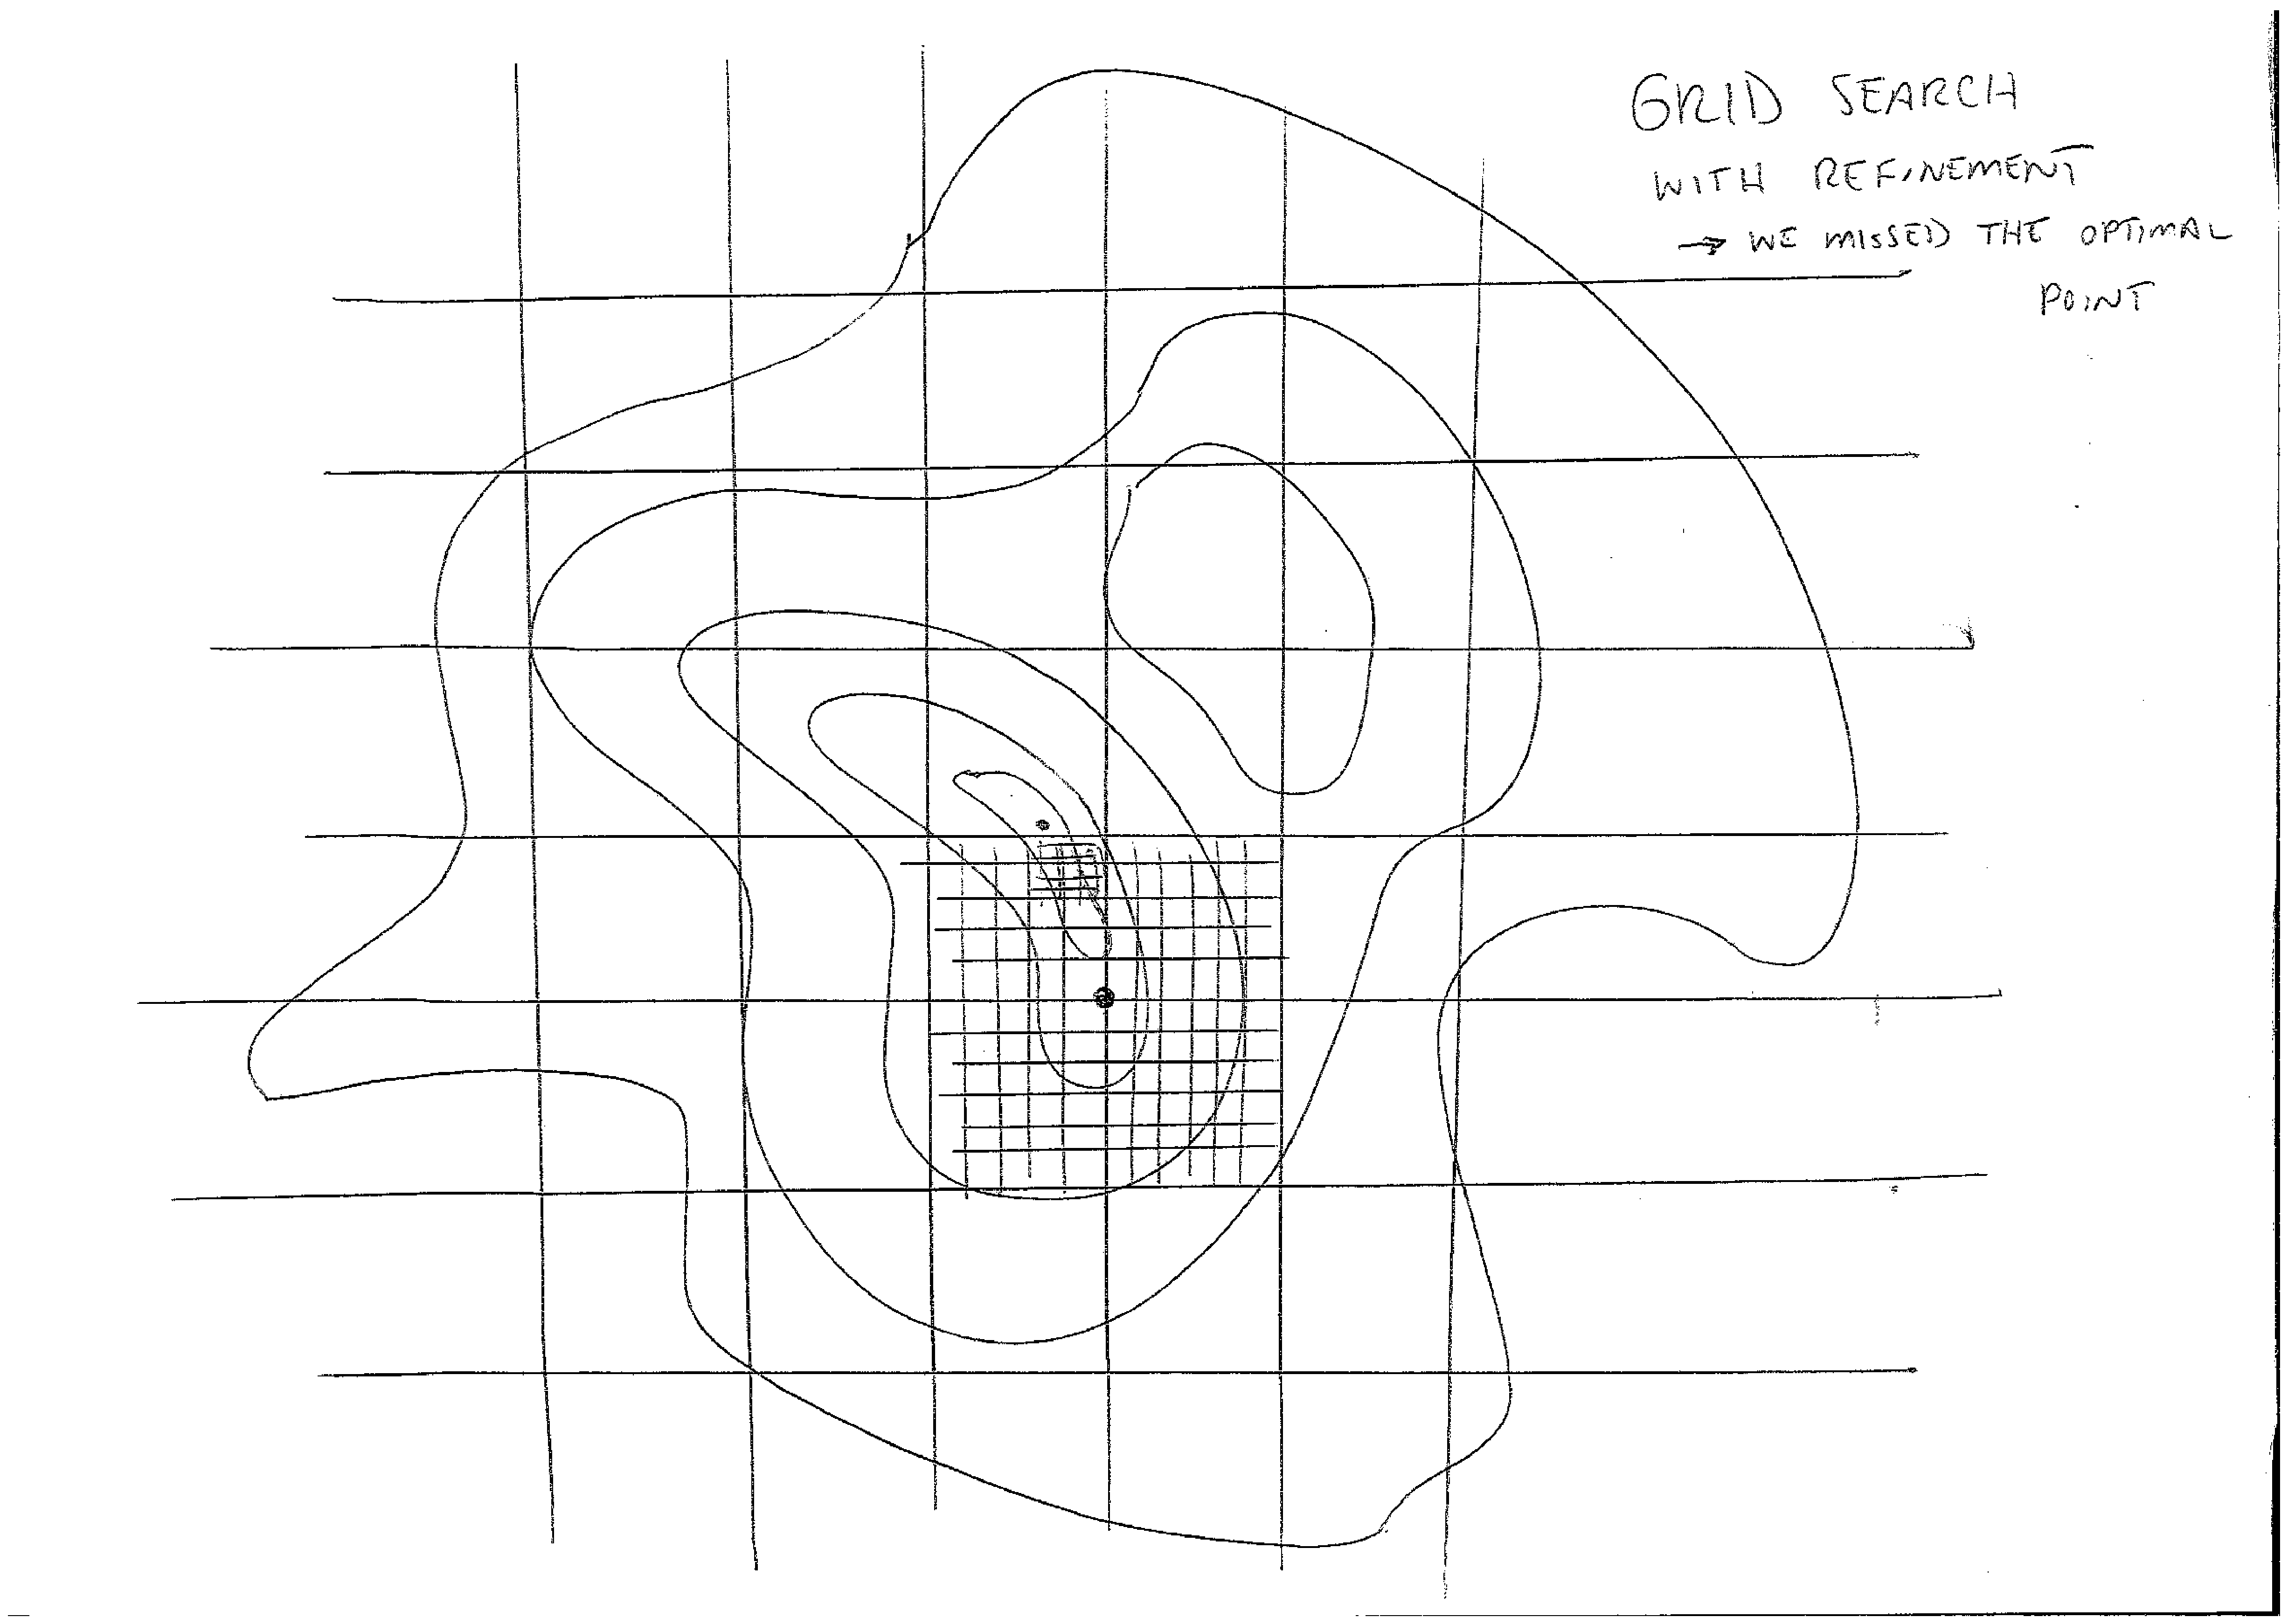
\includegraphics[width=15cm]{Examples/NonlinearOptimization/Search}

\end{figure}


To check $q$ values in each dimension of a $K$ dimensional parameter space, we need to check $q^{K}$ points. For example, if $q=100$ and $K=10,$ there would be $100^{10}$ points to check. If 1000 points can be checked in a second, it would take $3.\,171\times10^{9}$ years to perform the calculations, which is approximately 2/3 the age of the earth. The search method is a very reasonable choice if $K$ is small, but it quickly becomes infeasible if $K$ is moderate or large. 

The Octave function \htmladdnormallink{GridExample.m}{file:///home/michael/Mystuff/Econometrics/Examples/NonlinearOptimization/GridExample.m}  allows you to play around with a simple one dimensional grid search, selecting the number of evenly spaced values to try. Try running GridExample(5) and GridExample(10). The result of GridExample(10) is in Figure \ref{fig:Grid-search,-one}. In this example, we're in the neighborhood of the minimizer, but still not too close to the minimizer. However, we're close enough so refinement will lead us to converge to the global minimizer.

\begin{figure}
\caption{\label{fig:Grid-search,-one}Grid search, one dimension}


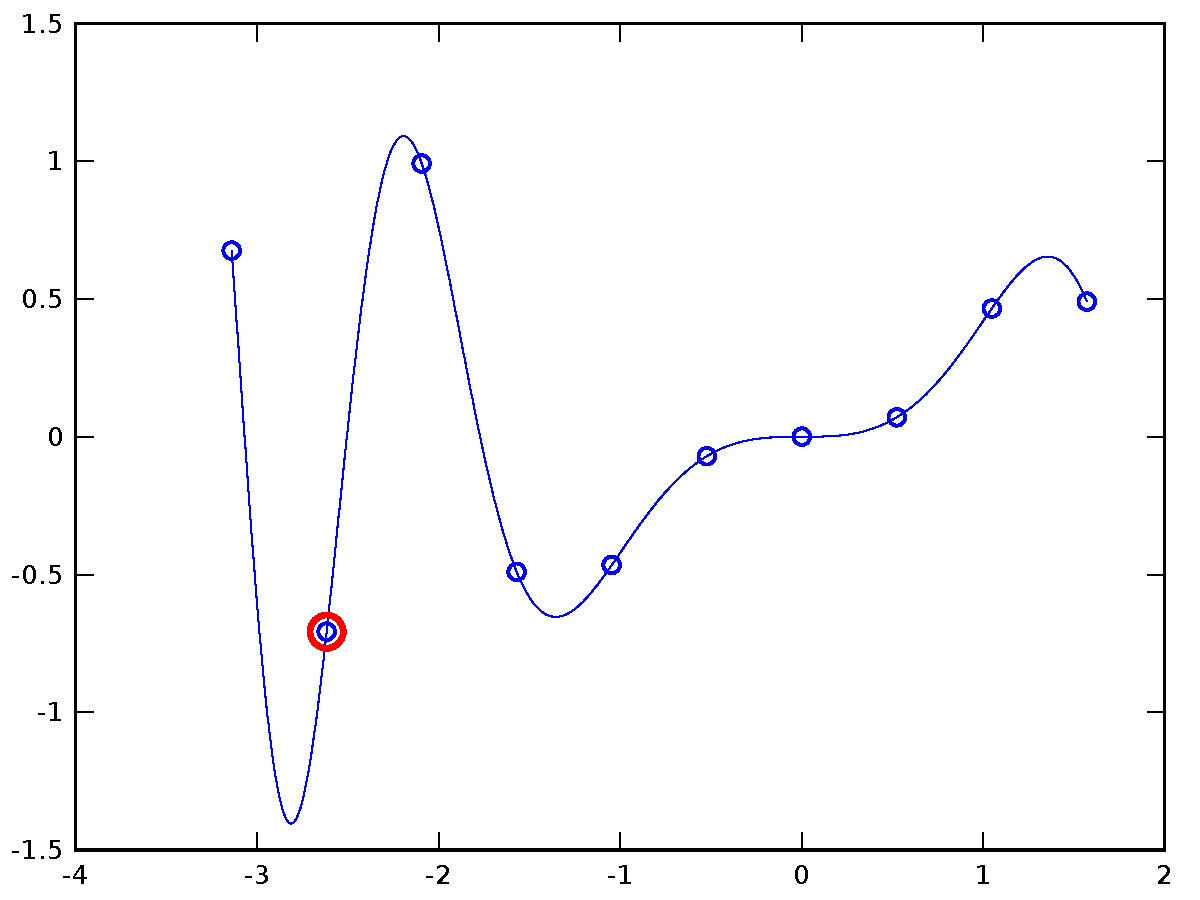
\includegraphics[width=15cm]{Examples/NonlinearOptimization/gridsearch}
\end{figure}
\newpage{}


\section{Derivative-based methods}


\subsection{Introduction}

\emph{In the following, $k$ is used as the index of the iterations of a given method. It is not an exponent, and it is not the dimension of the parameter vector.}

Derivative-based methods are defined by
\begin{enumerate}
\item the method for choosing the initial value, $\theta^{1}$
\item the iteration method for choosing $\theta^{k+1}$ given that we're at $\theta^{k}$ at iteration $k$ (based upon derivatives)
\item the stopping criterion. 
\end{enumerate}
The iteration method can be broken into two problems: choosing the stepsize $a^{k}$ (a scalar) and choosing the direction of movement, $d^{k},$ which is of the same dimension of $\theta,$ so that 
\[
\theta^{(k+1)}=\theta^{(k)}+a^{k}d^{k}.
\]


\emph{\newpage{}A locally increasing direction of search} $d$ is a direction such that 
\[
\frac{\partial s(\theta+ad)}{\partial a}>0
\]
 for $a$ positive but small. That is, if we go in direction $d$, we will improve on the objective function, at least if we don't go too far in that direction.
\begin{itemize}
\item As long as the gradient at $\theta$ is not zero, there exist increasing directions, and they can all be represented as $Q^{k}g(\theta^{k})$ where $Q^{k}$ is a symmetric pd matrix and $g\left(\theta\right)=D_{\theta}s(\theta)$ is the gradient at $\theta$. To see this, take a T.S. expansion around $a^{0}=0$
\begin{eqnarray*}
s(\theta+ad) & = & s(\theta+0d)+\left(a-0\right)g(\theta+0d)^{\prime}d+o(1)\\
 & = & s(\theta)+ag(\theta)^{\prime}d+o(1)
\end{eqnarray*}
 For small enough $a$ the $o(1)$ term can be ignored. If $d$ is to be an increasing direction, we need $g(\theta)^{\prime}d>0.$ Defining $d=Qg(\theta),$ where $Q$ is positive definite, we guarantee that 
\[
g(\theta)^{\prime}d=g(\theta)^{\prime}Qg(\theta)>0
\]
 unless $g(\theta)=0.$ Every increasing direction can be represented in this way (p.d. matrices are those such that the angle between $g$ and $Qg(\theta)$ is less than 90 degrees). See Figure \ref{Increasing directions}.\newpage{} 
\begin{figure}
\caption{\label{Increasing directions}Increasing directions of search}


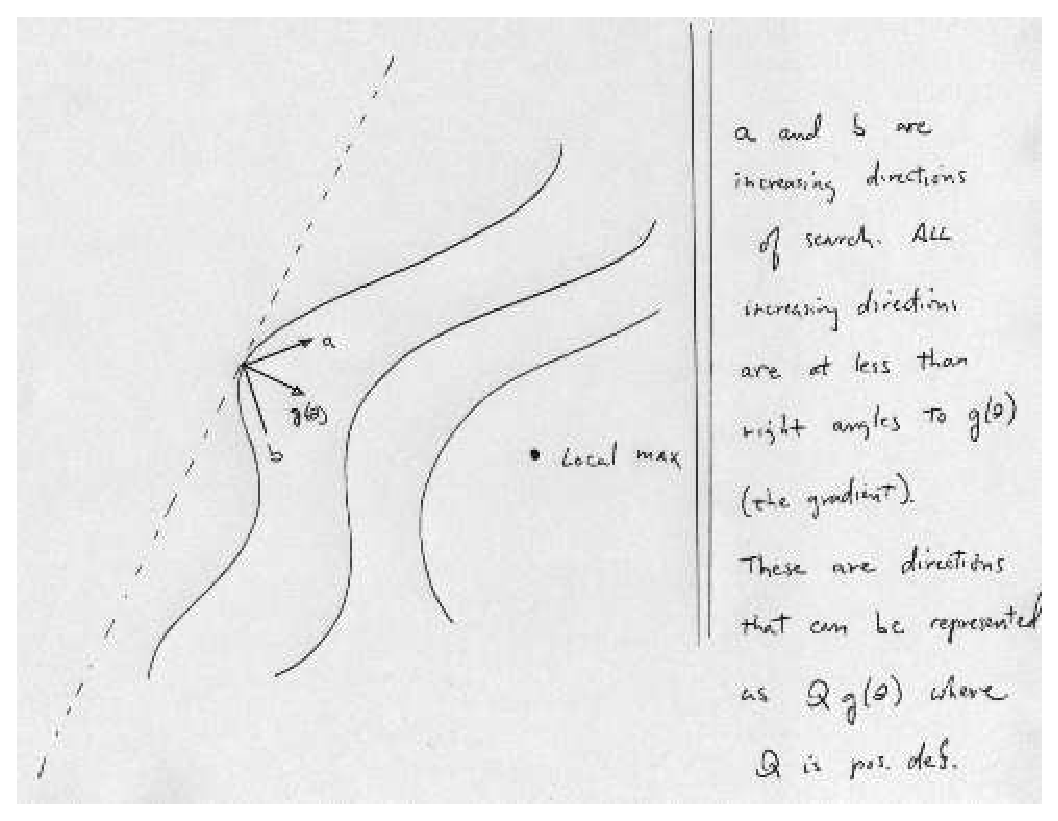
\includegraphics[width=6in]{Examples/NonlinearOptimization/IncreasingDirections}
\end{figure}
\newpage{}
\item With this, the iteration rule becomes 
\[
\theta^{(k+1)}=\theta^{(k)}+a^{k}Q^{k}g(\theta^{k})
\]

\end{itemize}
and we keep going until the gradient becomes zero, so that there is no increasing direction. The problem is how to choose $a$ and $Q.$
\begin{itemize}
\item \textbf{Conditional on} $Q$, choosing $a$ is fairly straightforward. A simple line search is an attractive possibility, since $a$ is a scalar. 
\item The remaining problem is how to choose $Q.$
\item Note also that this gives no guarantees to find a global maximum. \newpage{}
\end{itemize}

\subsection{Steepest descent}

Steepest descent (ascent if we're maximizing) just sets $Q$ to and identity matrix, since the gradient provides the direction of maximum rate of change of the objective function.
\begin{itemize}
\item Advantages:\ fast - doesn't require anything more than first derivatives.
\item Disadvantages: This doesn't always work too well however: see the Rosenbrock, or ''banana'' function: \url{http://en.wikipedia.org/wiki/Rosenbrock_function}.\newpage{}
\end{itemize}

\subsection{Newton' s method}

Newton's method uses information about the slope and curvature of the objective function to determine which direction and how far to move from an initial point. Supposing we're trying to maximize $s_{n}(\theta).$ Take a second order Taylor's series approximation of $s_{n}(\theta)$ about $\theta^{k}$ (an initial guess). 
\[
s_{n}(\theta)\approx s_{n}(\theta^{k})+g(\theta^{k})^{\prime}\left(\theta-\theta^{k}\right)+1/2\left(\theta-\theta^{k}\right)^{\prime}H(\theta^{k})\left(\theta-\theta^{k}\right)
\]
 To attempt to maximize $s_{n}(\theta),$ we can maximize the portion of the right-hand side that depends on $\theta,$ \emph{i.e.}, we can maximize 
\[
\tilde{s}(\theta)=g(\theta^{k})^{\prime}\theta+1/2\left(\theta-\theta^{k}\right)^{\prime}H(\theta^{k})\left(\theta-\theta^{k}\right)
\]
 with respect to $\theta.$ This is a much easier problem, since it is a quadratic function in $\theta,$ so it has linear first order conditions. These are

\[
D_{\theta}\tilde{s}(\theta)=g(\theta^{k})+H(\theta^{k})\left(\theta-\theta^{k}\right)
\]
 So the solution for the next round estimate is 
\[
\theta^{k+1}=\theta^{k}-H(\theta^{k})^{-1}g(\theta^{k})
\]
See \url{http://en.wikipedia.org/wiki/Newton%27s_method_in_optimization} for more information. This is illustrated in Figure \ref{fig:Newton-iteration}.

\begin{figure}


\caption{\label{fig:Newton-iteration}Newton iteration}


\includegraphics[width=15cm]{Examples/NonlinearOptimization/newton}

\end{figure}


However, it's good to include a stepsize, since the approximation to $s_{n}(\theta)$ may be bad far away from the maximizer $\hat{\theta},$ so the actual iteration formula is 
\[
\theta^{k+1}=\theta^{k}-a^{k}H(\theta^{k})^{-1}g(\theta^{k})
\]
\newpage{}
\begin{itemize}
\item A potential problem is that the Hessian may not be negative definite when we're far from the maximizing point. So $-H(\theta^{k})^{-1}$ may not be positive definite, and $-H(\theta^{k})^{-1}g(\theta^{k})$ may not define an increasing direction of search. This can happen when the objective function has flat regions, in which case the Hessian matrix is very ill-conditioned (e.g., is nearly singular), or when we're in the vicinity of a local minimum, $H(\theta^{k})$ is positive definite, and our direction is a \emph{decreasing} direction of search. Matrix inverses by computers are subject to large errors when the matrix is ill-conditioned. Also, we certainly don't want to go in the direction of a minimum when we're maximizing. To solve this problem, \emph{Quasi-Newton} methods simply add a positive definite component to $H(\theta)$ to ensure that the resulting matrix is positive definite, \emph{e.g.,} $Q=-H(\theta)+b\mathbf{I},$ where $b$ is chosen large enough so that $Q$ is well-conditioned and positive definite. This has the benefit that improvement in the objective function is guaranteed. See \url{http://en.wikipedia.org/wiki/Quasi-Newton_method}.
\item Another variation of quasi-Newton methods is to approximate the Hessian by using successive gradient evaluations. This avoids actual calculation of the Hessian, which is an order of magnitude (in the dimension of the parameter vector) more costly than calculation of the gradient. They can be done to ensure that the approximation is p.d. DFP\ and BFGS are two well-known examples. 
\item show bfgsmin\_example.m to optimize Rosenbrock function\newpage{}
\end{itemize}
\textbf{Stopping criteria}

The last thing we need is to decide when to stop. A digital computer is subject to limited machine precision and round-off errors. For these reasons, it is unreasonable to hope that a program can \textbf{exactly} find the point that maximizes a function. We need to define acceptable tolerances. Some stopping criteria are:
\begin{itemize}
\item Negligible change in parameters: 
\[
|\theta_{j}^{k}-\theta_{j}^{k-1}|<\varepsilon_{1},\forall j
\]

\item Negligible relative change: 
\[
|\frac{\theta_{j}^{k}-\theta_{j}^{k-1}}{\theta_{j}^{k-1}}|<\varepsilon_{2},\forall j
\]

\item Negligible change of function: 
\[
|s(\theta^{k})-s(\theta^{k-1})|<\varepsilon_{3}
\]

\item Gradient negligibly different from zero: 
\[
|g_{j}(\theta^{k})|<\varepsilon_{4},\forall j
\]

\item Or, even better, check all of these.
\item Also, if we're maximizing, it's good to check that the last round (real, not approximate) Hessian is negative definite. 
\end{itemize}
\newpage{}\textbf{Starting values}

The Newton-Raphson and related algorithms work well if the objective function is concave (when maximizing), but not so well if there are convex regions and local minima or multiple local maxima. The algorithm may converge to a local minimum or to a local maximum that is not optimal. The algorithm may also have difficulties converging at all.
\begin{itemize}
\item The usual way to ``ensure'' that a global maximum has been found is to use many different starting values, and choose the solution that returns the highest objective function value. \textbf{THIS\ IS\ IMPORTANT in practice.} More on this later.
\item an alternative is to use a global optimization algorithm, e.g., simulated annealing or others, which may or may not be gradient based.
\end{itemize}
\newpage{}\textbf{Calculating derivatives}

The Newton-Raphson algorithm requires first and second derivatives. It is often difficult to calculate derivatives (especially the Hessian) analytically if the function $s_{n}(\cdot)$ is complicated. Possible solutions are to calculate derivatives numerically, or to use programs such as MuPAD or Mathematica to calculate analytic derivatives. For example, Figure \ref{fig:Using-Sage-to} shows Sage \footnote{Sage is free software that has both symbolic and numeric computational capabilities. See \url{http://www.sagemath.org/}} calculating a couple of derivatives. The KAIST Sage cell server will let you try Sage online, its address is \url{http://aleph.sagemath.org/}.\newpage{}
\begin{figure}
\caption{\label{fig:Using-Sage-to}Using Sage to get analytic derivatives}


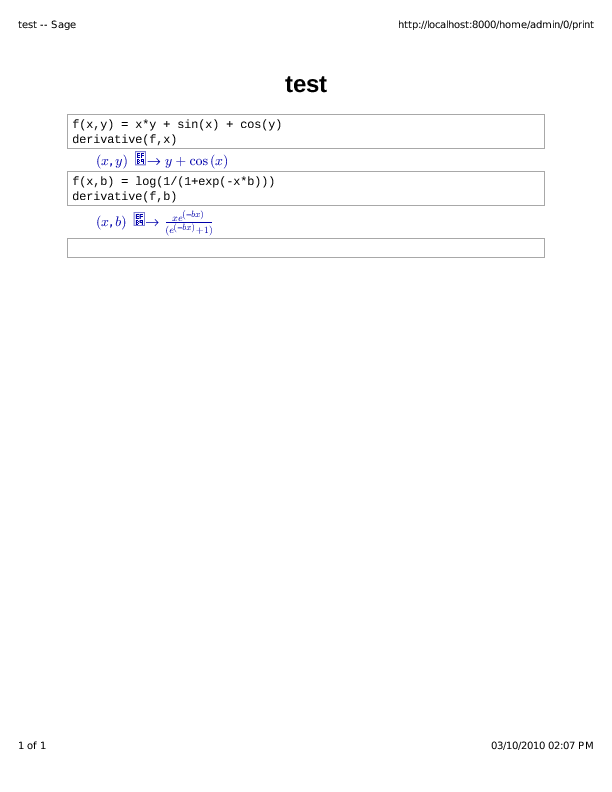
\includegraphics[width=15cm]{/home/michael/Mystuff/Econometrics/Examples/NonlinearOptimization/sage}
\end{figure}
\newpage{}
\begin{itemize}
\item Numeric derivatives are less accurate than analytic derivatives, and are usually more costly to evaluate. Both factors usually cause optimization programs to be less successful when numeric derivatives are used. 
\item One advantage of numeric derivatives is that you don't have to worry about having made an error in calculating the analytic derivative. When programming analytic derivatives it's a good idea to check that they are correct by using numeric derivatives. This is a lesson I learned the hard way when writing my thesis.
\item there are also methods for \emph{automatic differentiation}. This will probably become important in the future, but existing econometric software makes little use of it.\newpage{}
\item Numeric second derivatives are much more accurate if the data are scaled so that the elements of the gradient are of the same order of magnitude. Example: if the model is $y_{t}=h(\alpha x_{t}+\beta z_{t})+\varepsilon_{t},$ and estimation is by NLS. Let $g()$ be the derivative of $h().$

\begin{itemize}
\item so, $s_{n}(\theta)=\frac{1}{n}\sum_{t}\left(y_{t}-h(\alpha x_{t}+\beta z_{t})\right)^{2}$ and
\item $D_{\alpha}s_{n}(\cdot)=\frac{1}{n}\sum_{t}2\left(y_{t}-h(\alpha x_{t}+\beta z_{t})\right)g(\alpha x_{t}+\beta z_{t})x_{t}$. 
\item $D_{\beta}s_{n}(\cdot)=\frac{1}{n}\sum_{t}2\left(y_{t}-h(\alpha x_{t}+\beta z_{t})\right)g(\alpha x_{t}+\beta z_{t})z_{t}$
\item suppose that $D_{\alpha}s_{n}(\cdot)=1000$ and $D_{\beta}s_{n}(\cdot)=0.001.$ One could define $\alpha^{\ast}=1000\alpha;$ $x_{t}^{\ast}=x_{t}/1000$;$\beta^{\ast}=\beta/1000;z_{t}^{\ast}=1000z_{t}.$ 
\item then $D_{\alpha^{*}}s_{n}(\cdot)=\frac{1}{n}\sum_{t}2\left(y_{t}-h(\alpha^{*}x_{t}^{*}+\beta^{*}z_{t}^{*})\right)g(\alpha^{*}x_{t}^{*}+\beta^{*}z_{t}^{*})x_{t}^{*}$. Everything is the same as before, except there is an $x_{t}^{*}$ at the end, which causes the derivative to be 1 now.
\item the same is true for the other derivative, it will be 1.
\item this scaling causes the derivatives to be of the same order.
\end{itemize}

In general, estimation programs always work better if data is scaled in this way, since roundoff errors are less likely to become important. \emph{This is important in practice. }In the future, if you start to do empirical work and get results that seem meaningless or crazy, try to remember this point.\newpage{}

\item There are algorithms (such as BFGS and DFP) that use the sequential gradient evaluations to build up an approximation to the Hessian. The iterations are faster because the actual Hessian isn't calculated, but more iterations usually are required for convergence. Versions of BFGS are probably the most widely used optimizers in econometrics.
\item Switching between algorithms during iterations is sometimes useful. \newpage{}\end{itemize}
\begin{example}
The Nerlove model via numeric minimization. The example code \htmladdnormallink{EstimateRestrictedNerlove.m}{file:///home/michael/Mystuff/Econometrics/Examples/NonlinearOptimization/EstimateRestrictedNerlove.m}  shows how to use unconstrained and constrained minimization to estimate the simple Nerlove model (equation \ref{simple nerlove model}) with and without parameter restrictions.\newpage{}
\end{example}

\section{Simulated Annealing}

Simulated annealing is an algorithm which can find an optimum in the presence of nonconcavities, discontinuities and multiple local minima/maxima. Basically, the algorithm randomly selects evaluation points, accepts all points that yield an increase in the objective function, but also accepts some points that decrease the objective function. This allows the algorithm to escape from local minima. As more and more points are tried, periodically the algorithm focuses on the best point so far, and reduces the range over which random points are generated. Also, the probability that a negative move is accepted reduces. The algorithm relies on many evaluations, as in the search method, but focuses in on promising areas, which reduces function evaluations with respect to the search method. It does not require derivatives to be evaluated. Run samin\_example.m if you're using the live CD image, or enter Octave and type edit samin.cc to see the code.\newpage{}


\section{\label{sub:MEPS data}A practical example: Maximum likelihood estimation using count data: The MEPS data and the Poisson model}

To show optimazation methods in practice, using real economic data, this section presents maximum likelihood estimation results for a particular model using real data. The focus at present is simply on numeric optimization. Later, after studying maximum likelihood estimation, this section can be read again.

Demand for health care is usually thought of a a derived demand: health care is an input to a home production function that produces health, and health is an argument of the utility function. Grossman (1972), for example, models health as a capital stock that is subject to depreciation (e.g., the effects of ageing). Health care visits restore the stock. Under the home production framework, individuals decide when to make health care visits to maintain their health stock, or to deal with negative shocks to the stock in the form of accidents or illnesses. As such, individual demand will be a function of the parameters of the individuals' utility functions.

\label{The-,-meps1996.data,}The \htmladdnormallink{MEPS health data file}{file:///home/michael/Mystuff/Econometrics/Examples/Data/meps1996.data} , \texttt{meps1996.data,} contains 4564 observations on six measures of health care usage. The data is from the 1996 Medical Expenditure Panel Survey (MEPS). You can get more information at \url{http://www.meps.ahrq.gov/}. The six measures of use are are office-based visits (OBDV), outpatient visits (OPV), inpatient visits (IPV), emergency room visits (ERV), dental visits (VDV), and number of prescription drugs taken (PRESCR). These form columns 1 - 6 of \texttt{meps1996.data}. The conditioning variables are public insurance (PUBLIC), private insurance (PRIV), sex (SEX), age (AGE), years of education (EDUC), and income (INCOME). These form columns 7 - 12 of the file\texttt{,} in the order given here. PRIV and PUBLIC are 0/1 binary variables, where a 1 indicates that the person has access to public or private insurance coverage. SEX is also 0/1, where 1 indicates that the person is female. This data will be used in examples fairly extensively in what follows.

The program \htmladdnormallink{ExploreMEPS.m}{file:///home/michael/Mystuff/Econometrics/Examples/MEPS-I/ExploreMEPS.m}  shows how the data may be read in, and gives some descriptive information about variables, which follows:\verbatiminput{MEPS-I/MepsStats.out}

All of the measures of use are count data, which means that they take on the values ${0,1,2,...}$. It might be reasonable to try to use this information by specifying the density as a count data density. One of the simplest count data densities is the Poisson density, which is
\begin{eqnarray*}
f_{Y}(y) & = & \frac{\exp(-\lambda)\lambda^{y}}{y!}.
\end{eqnarray*}
For this density, $E(Y)=V(Y)=\lambda$. The Poisson average log-likelihood function is 
\[
s_{n}(\theta)=\frac{1}{n}\sum_{i=1}^{n}\left(-\lambda_{i}+y_{i}\ln\lambda_{i}-\ln y_{i}!\right)
\]
We will parameterize the model as
\begin{eqnarray}
\lambda_{i} & = & \exp(\mathbf{x}_{i}^{\prime}\beta)\nonumber \\
\mathbf{x}_{i} & = & [1\,\,PUBLIC\,\,PRIV\,\,SEX\,\,AGE\,\,EDUC\,\,INC]^{\prime}\label{eq:Poisson model OBDV}
\end{eqnarray}
This ensures that the mean is positive, as is required for the Poisson model, and now the mean (and the variance) depend upon explanatory variables. Note that for this parameterization
\[
\frac{\partial\lambda}{\partial x_{j}}=\lambda\beta_{j}
\]
so

\[
\beta_{j}x_{j}=\frac{\partial\lambda}{\partial x_{j}}\frac{x_{j}}{\lambda}=\eta_{x_{j}}^{\lambda},
\]
the elasticity of the conditional mean of $y$ with respect to the $j^{th}$ conditioning variable.

The program  \htmladdnormallink{EstimatePoisson.m}{file:///home/michael/Mystuff/Econometrics/Examples/MEPS-I/EstimatePoisson.m} estimates a Poisson model using the full data set. The results of the estimation, using OBDV as the dependent variable are here: \label{OBDV ML results}\verbatiminput{Examples/MEPS-I/PoissonOBDV.out}\label{PoissonOBDV_results}


\section{Numeric optimization: pitfalls}

In this section we'll examine two common problems that can be encountered when doing numeric optimization of nonlinear models, and some solutions.


\subsection{Poor scaling of the data}

When the data is scaled so that the magnitudes of the first and second derivatives are of different orders, problems can easily result. If we uncomment the appropriate line in  \htmladdnormallink{EstimatePoisson.m}{file:///home/michael/Mystuff/Econometrics/Examples/MEPS-I/EstimatePoisson.m}, the data will not be scaled, and the estimation program will have difficulty converging (it seems to take an infinite amount of time). With unscaled data, the elements of the score vector have very different magnitudes at the initial value of $\theta$ (all zeros). To see this run  \htmladdnormallink{CheckScore.m}{file:///home/michael/Mystuff/Econometrics/Examples/MEPS-I/CheckScore.m}. With unscaled data, one element of the gradient is very large, and the maximum and minimum elements are 5 orders of magnitude apart. This causes convergence problems due to serious numerical inaccuracy when doing inversions to calculate the BFGS direction of search. With scaled data, none of the elements of the gradient are very large, and the maximum difference in orders of magnitude is 3. Convergence is quick.


\subsection{Multiple optima}

Multiple optima (one global, others local) can complicate life, since we have limited means of determining if there is a higher maximum than the one we're at. Think of climbing a mountain in an unknown range, in a very foggy place. A nice picture is Figure \ref{foggy mountain-1}, but try to imagine the scene if the clouds were 2000m thicker. A representation is Figure \ref{foggy mountain}). You can go up until there's nowhere else to go up, but since you're in the fog you don't know if the true summit is across the gap that's at your feet. Do you claim victory and go home, or do you trudge down the gap and explore the other side?

\begin{figure}
\caption{\label{foggy mountain-1}Mountains with low fog}


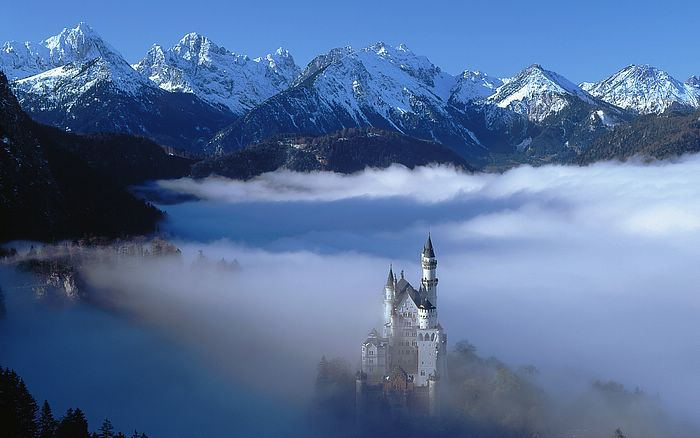
\includegraphics[width=6in]{Examples/Figures/mountain}
\end{figure}


\begin{figure}
\caption{\label{foggy mountain}A foggy mountain}


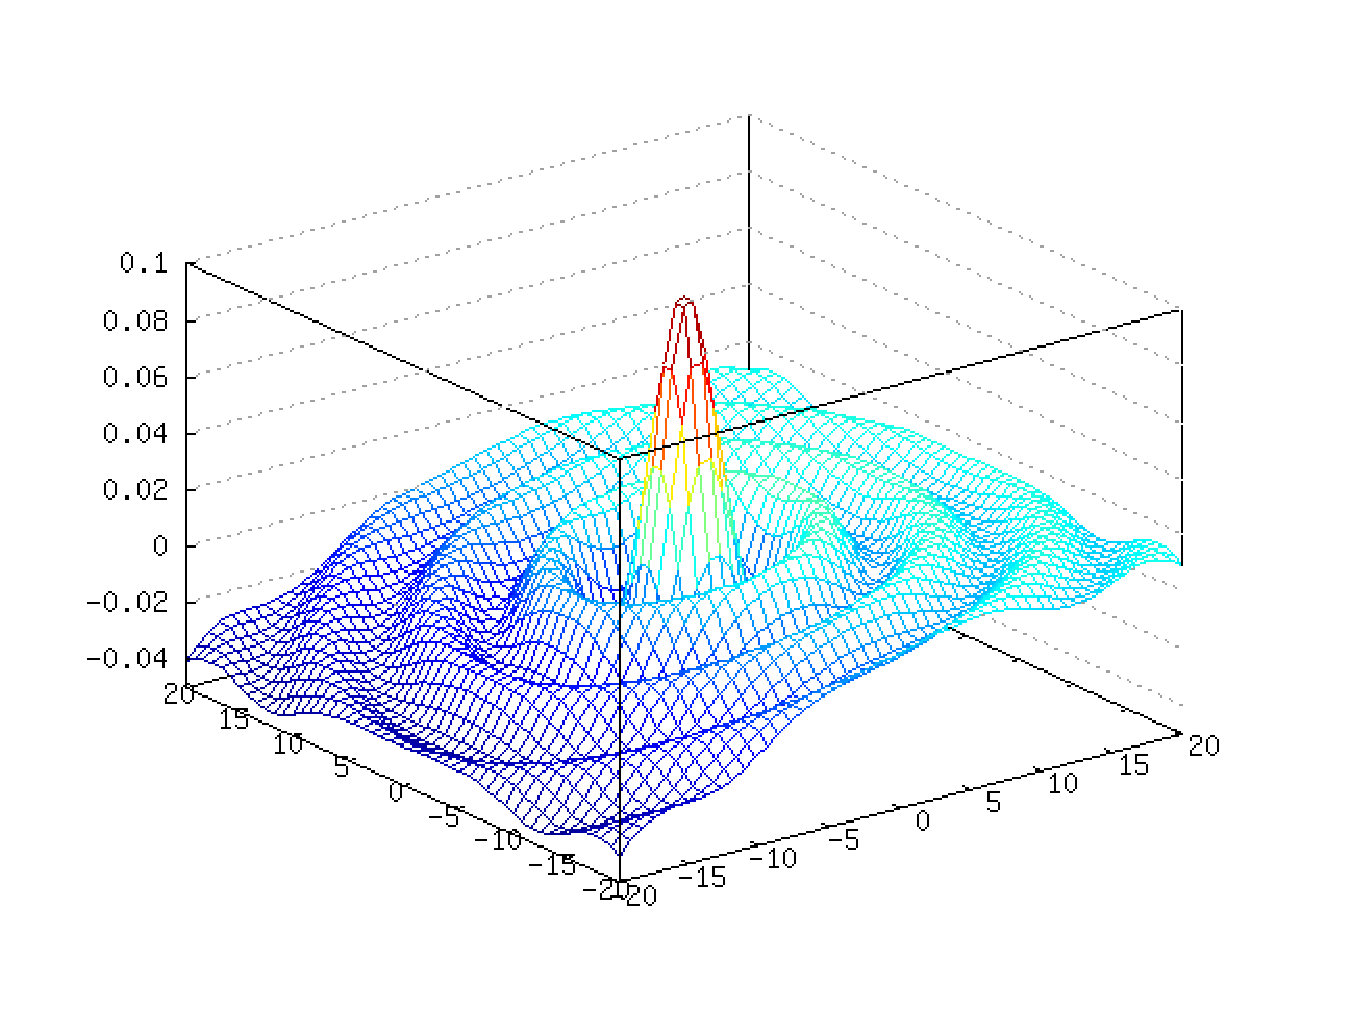
\includegraphics[width=6in]{/home/michael/Mystuff/Econometrics/Examples/NonlinearOptimization/FoggySurface}
\end{figure}


The best way to avoid stopping at a local maximum is to use many starting values, for example on a grid, or randomly generated. Or perhaps one might have priors about possible values for the parameters (\emph{e.g.,} from previous studies of similar data).

Let's try to find the true minimizer of minus 1 times the foggy mountain function (since the algorithms are set up to minimize). From the picture, you can see it's close to $(0,0)$, but let's pretend there is fog, and that we don't know that. The program  \htmladdnormallink{FoggyMountain.m}{file:///home/michael/Mystuff/Econometrics/Examples/NonlinearOptimization/FoggyMountain.m} shows that poor start values can lead to problems. It uses SA, which finds the true global minimum, and it shows that BFGS using a battery of random start values can also find the global minimum help. The output of one run is here: \verbatiminput{Examples/NonlinearOptimization/FoggyMountain.out}In that run, the single BFGS run with bad start values converged to a point far from the true minimizer, which simulated annealing and BFGS using a battery of random start values both found the true maximizer. Using a battery of random start values, we managed to find the global max. The moral of the story is to be cautious and don't publish your results too quickly.

\newpage{}


\section{Exercises}
\begin{enumerate}
\item In octave, type ''\texttt{help bfgsmin\_example}'', to find out the location of the file. Edit the file to examine it and learn how to call \texttt{bfgsmin}. Run it, and examine the output.
\item In octave, type ''\texttt{help samin\_example}'', to find out the location of the file. Edit the file to examine it and learn how to call \texttt{samin}. Run it, and examine the output.
\item Numerically minimize the function $\sin(x)+0.01\left(x-a\right)^{2}$, setting $a=0$, using the software of your choice. Plot the function over the interval $\left(-2\pi,2\pi\right)$. Does the software find the global minimum? Does this depend on the starting value you use? Outline a strategy that would allow you to find the minimum reliably, when $a$ can take on any given value in the interval $\left(-\pi,\pi\right)$.
\item Numerically compute the OLS estimator of the Nerlove model by using an interative minimization algorithm to minimize the sum of squared residuals. Verify that the results coincide with those given in subsection \ref{sub:The-Nerlove-data}. The important part of this problem is to learn how to minimize a function that depends on both parameters and data. Try to write your function so that it is easy to use it with an arbitrary data set.
\item Numerically compute the OLS estimator of the Nerlove model 
\[
\ln C=\beta+\beta_{Q}\ln Q+\beta_{L}\ln P_{L}+\beta_{F}\ln P_{F}+\beta_{K}\ln P_{K}+\epsilon
\]
by using Octave's (or Matlab's) fminunc to minimize the sum of squared residuals. The data is at the link \htmladdnormallink{nerlove.data}{file:///home/michael/Mystuff/Econometrics/Examples/Data/nerlove.data}  . Verify that the results coincide with those given in subsection \ref{sub:The-Nerlove-data}, or with what you get from GRETL, i.e.: %%% the following needs the amsmath LaTeX package
\begin{gather} \begin{split} \widehat{\rm l\_cost} &= -\underset{(1.7744)}{3.52650} +\underset{(0.017466)}{0.720394}\,\mbox{l\_output} +\underset{(0.29105)}{0.436341}\,\mbox{l\_labor} +\underset{(0.10037)}{0.426517}\,\mbox{l\_fuel}\\ & -\underset{(0.33943)}{0.219888}\,\mbox{l\_capital} \end{split} \notag \\ T = 145 \quad \bar{R}^2 = 0.9238 \quad F(4,140) = 437.69 \quad \hat{\sigma} = 0.39236 \notag \\ \centerline{(standard errors in parentheses)} \notag \end{gather} The important part of this problem is to learn how to minimize a function that depends on both parameters and data. Try to write your function so that it is re-usable, with a different data set. 
\item Suppose we have an $AR(1)$ model $y_{t}=\rho y_{t-1}+u_{t}$. Suppose that $y_{t}$ is stationary, and that the error $u_{t}$ is white noise. Explain how one could compute an estimator of $\rho$ using the grid search method. You must define your criterion function and explain how to implement the grid search. \newpage{}
\end{enumerate}

\chapter{\label{cha:Asymptotic-properties-of}Asymptotic properties of extremum estimators}

\textbf{Readings}: Cameron and Trivedi, Ch. 5; Hayashi (2000), Ch. 7; Gourieroux and Monfort (1995), Vol. 2, Ch. 24; Amemiya, Ch. 4 section 4.1; Davidson and MacKinnon, pp. 591-96; Gallant, Ch. 3; Newey and McFadden (1994), ``\href{http://www.sciencedirect.com/science?_ob=ArticleURL&_udi=B7GX7-4FPWV09-5&_user=1517286&_coverDate=12\%2F31\%2F1994&_rdoc=5&_fmt=high&_orig=browse&_srch=doc-info(\%23toc\%2320479\%231994\%23999959999\%23583590\%23FLP\%23display\%23Volume)&_cdi=20479&_sort=d&_docanchor=&_ct=21&_acct=C000053449&_version=1&_urlVersion=0&_userid=1517286&md5=5a540eb9d22288a9f25f3914db38aa1b}{Large Sample Estimation and Hypothesis Testing},'' in \emph{\href{http://www.sciencedirect.com/science/handbooks/15734412}{Handbook of Econometrics}, Vol. 4}, Ch. 36.\newpage{}


\section{Extremum estimators}

We'll begin with study of \emph{extremum estimators} in general. Let $\mathbf{Z}_{n}=\left\{ z_{1},z_{2},...,z_{n}\right\} $ be the available data, arranged in a $n\times p$ matrix, based on a sample of size $n$ (there are $p$ variables). Our paradigm is that data are generated as a draw from the joint density $f_{Z_{n}}(z)$. This density may not be known, but it exists in principle. The draw from the density may be thought of as the outcome of a random experiment that is characterized by the probability space $\left\{ \Omega,\mathcal{F},P\right\} $. When the experiment is performed, $\omega\in\Omega$ is the result, and $\mathbf{Z}_{n}(\omega)=\left\{ Z_{1}(\omega),Z_{2}(\omega),...,Z_{n}(\omega)\right\} =\left\{ z_{1},z_{2},...,z_{n}\right\} $ is the realized data. The probability space is rich enough to allow us to consider events defined in terms of an infinite sequence of data $\mathbf{Z}=\left\{ z_{1},z_{2},...,\right\} $.\newpage{}
\begin{defn}
{[}Extremum estimator{]} \label{Extremum estimator}An extremum estimator\index{extremum estimator} $\hat{\theta}$ is the optimizing element of an objective function $s_{n}(\mathbf{Z}_{n},\theta)$ over a set $\overline{\Theta}$. 
\end{defn}
Because the data $\mathbf{Z}_{n}(\omega)$ depends on $\omega$, we can emphasize this by writing $s_{n}(\omega,\theta)$. I'll be loose with notation and interchange when convenient.\newpage{}
\begin{example}
OLS. Let the d.g.p. be $y_{t}=\mathbf{x}_{t}^{\prime}\theta^{0}+\varepsilon_{t},\,t=1,2,...,n,\,\theta^{0}\in\Theta.$ Stacking observations vertically, $\mathbf{y}_{n}=\mathbf{X}_{n}\theta^{0}+\varepsilon_{n},$ where $\mathbf{X}_{n}=\left(\begin{array}{llll}
x_{1} & x_{2} & \cdots & x_{n}\end{array}\right)^{\prime}.$ Let $\mathbf{Z}_{n}=[\mathbf{y}_{n}\,\mathbf{X}_{n}]$. The least squares estimator is defined as 
\[
\hat{\theta}\equiv\arg\min_{\Theta}s_{n}(\mathbf{Z}_{n},\theta)
\]
where 
\[
s_{n}(\mathbf{Z}_{n},\theta)=1/n\sum_{t=1}^{n}\left(y_{t}-\mathbf{x}_{t}^{\prime}\theta\right)^{2}
\]
 As you already know, $\hat{\theta}=(\mathbf{X}^{\prime}\mathbf{X})^{-1}\mathbf{X}^{\prime}\mathbf{y}.$\newpage{}

Maximum likelihood. Suppose that the continuous random variables $Y_{t}\sim IIN(\theta^{0},\sigma_{0}^{2}),\,t=1,2,...,n$. If $\epsilon$ is a standard normal random variable, its density is 
\[
f_{\epsilon}(z;\theta)=\left(2\pi\right)^{-1/2}\exp\left(-\frac{z^{2}}{2}\right).
\]
 We have that $\epsilon_{t}=(Y_{t}-\theta_{0})/\sigma_{0}$ is standard normal, and the Jacobian $\left|\partial\epsilon_{t}/\partial y_{t}\right|=1/\sigma_{0}$. Thus, doing a change of variable, the density of a single observation on $Y$ is
\[
f_{Y}(y_{t};\theta,\sigma)=\left(2\pi\right)^{-1/2}(1/\sigma)\exp\left(-\frac{1}{2}\left(\frac{y_{t}-\theta}{\sigma}\right)^{2}\right).
\]
The maximum likelihood estimator is maximizes the joint density of the sample. Because the data are i.i.d., the joint density of the sample $\left\{ y_{1},y_{2},...,y_{n}\right\} $ is the product of the densities of each observation, and the ML estimator is 
\[
\hat{\theta}\equiv\arg\max_{\Theta}\,\,\mathcal{L}_{n}(\theta)=\prod_{t=1}^{n}\left(2\pi\right)^{-1/2}(1/\sigma)\exp\left(-\frac{\left(y_{t}-\theta\right)^{2}}{2}\right)
\]
Because the natural logarithm is strictly increasing on $(0,\infty)$, maximization of the average logarithmic likelihood function is achieved at the same $\hat{\theta}$ as for the likelihood function. So, the ML estimator $\hat{\theta}\equiv\arg\max_{\Theta}s_{n}(\theta)$ where 
\[
s_{n}(\theta)=\left(1/n\right)\ln\mathcal{L}_{n}(\theta)=-\ln\sqrt{2\pi}-\text{\ensuremath{\log}}\sigma-\left(1/n\right)\sum_{t=1}^{n}\frac{\left(y_{t}-\theta\right)^{2}}{2}
\]
Solution of the f.o.c. leads to the familiar result that $\hat{\theta}=\bar{\mathbf{y}}.$ We'll come back to this in more detail later.
\end{example}
\newpage{}
\begin{example}
Bayesian estimator

(reminder to self in lectures: that squiggle is a ''zeta'') Bayesian point estimators such as the posterior mode, median or mean can be expressed as extremum estimators. For example, the posterior mean $E(\theta|Z_{n})$ is the minimizer (with respect to $\zeta$) of the function
\[
s_{n}(\zeta)=\int_{\Theta}\left(\theta-\zeta\right)^{2}f(Z_{n};\theta)\pi(\theta)/f(Z_{n})d\theta
\]

\end{example}
where $f(Z_{n};\theta)$ is the likelihood function, $\pi(\theta)$ is a prior density, and $f(Z_{n})$ is the marginal likelihood of the data. These concepts are explained later, for now the point is that Bayesian estimators can be thought of as extremum estimators, and the theory for extremum estimators will apply.

\newpage{}

Note that the objective function $s_{n}(\mathbf{Z}_{n},\theta)$ is a random function, because it depends on $\mathbf{Z}_{n}(\omega)=\left\{ Z_{1}(\omega),Z_{2}(\omega),...,Z_{n}(\omega)\right\} =\left\{ z_{1},z_{2},...,z_{n}\right\} $. We need to consider what happens as different outcomes $\omega\in\Omega$ occur. These different outcomes lead to different data being generated, and the different data causes the objective function to change. Note, however, that for a fixed $\omega\in\Omega$, the data $\mathbf{Z}_{n}(\omega)=\left\{ Z_{1}(\omega),Z_{2}(\omega),...,Z_{n}(\omega)\right\} =\left\{ z_{1},z_{2},...,z_{n}\right\} $ are a fixed realization, and the objective function $s_{n}(\mathbf{Z}_{n},\theta)$ becomes a non-random function of $\theta$. When actually computing an extremum estimator, we treat the data as fixed, and employ algorithms for optimization of nonstochastic functions. When analyzing the properties of an extremum estimator, we need to investigate what happens throughout $\Omega$: we do not focus only on the $\omega$ that generated the observed data. This is because we would like to find estimators that work well on average for any data set that can result from $\omega\in\Omega$.

We'll often write the objective function suppressing the dependence on $\mathbf{Z}_{n},$ as $s_{n}(\omega,\theta)$ or simply $s_{n}(\theta)$, depending on context. The first of these emphasizes the fact that the objective function is random, and the second is more compact. However, the data is still in there, and because the data is randomly sampled, the objective function is random, too. \newpage{}


\section{Existence}

If $s_{n}(\theta)$ is continuous in $\theta$ and $\overline{\Theta}$ is compact, then a maximizer exists, by the Weierstrass maximum theorem (Debreu, 1959). In some cases of interest, $s_{n}(\theta)$ may not be continuous. Nevertheless, it may still converge to a continous function, in which case existence will not be a problem, at least asymptotically. Henceforth in this course, we assume that $s_{n}(\theta)$ is continuous.\newpage{}


\section{Consistency}

The following theorem is patterned on a proof in Gallant (1987) (the article, ref. later), which we'll see in its original form later in the course. It is interesting to compare the following proof with Amemiya's Theorem 4.1.1, which is done in terms of convergence in probability.
\begin{thm}
\emph{{[}Consistency of e.e.{]}} \label{Consistency of ee}Suppose that $\hat{\theta}_{n}$ is obtained by maximizing $s_{n}(\theta)$ over $\overline{\Theta}.$

Assume

(a) Compactness: The parameter space $\Theta$ is an open bounded subset of Euclidean space $\Re^{K}.$ So the closure of $\Theta,$ $\overline{\Theta}$, is compact.

(b) Uniform Convergence: There is a nonstochastic function $s_{\infty}(\theta)$ that is continuous in $\theta$ on $\overline{\Theta}$ such that 
\[
\lim_{n\rightarrow\infty}\sup_{\theta\in\overline{\Theta}}|s_{n}(\omega,\theta)-s_{\infty}(\theta)|=0,\,\text{a.s.}
\]


(c) Identification: $s_{\infty}(\cdot)$ has a unique global maximum at $\theta^{0}\in\Theta,$ i.e., $s_{\infty}(\theta^{0})>s_{\infty}(\theta),$ $\forall\theta\neq\theta^{0},\theta\in\overline{\Theta}$

Then $\hat{\theta}_{n}\stackrel{a.s.}{\rightarrow}\theta^{0}.$
\end{thm}
\newpage{}

\textbf{Proof:} 
\begin{itemize}
\item Select a $\omega\in\Omega$ and hold it fixed. Then $\left\{ s_{n}(\omega,\theta)\right\} $ is a fixed sequence of functions. Suppose that $\omega$ is such that $s_{n}(\omega,\theta)$ converges to $s_{\infty}(\theta).$ This happens with probability one by assumption (b). 
\item The sequence $\{\hat{\theta}_{n}\}$ lies in the compact set $\overline{\Theta},$ by assumption (a) and the fact that maximixation is over $\overline{\Theta}$. Since every sequence from a compact set has at least one limit point (Bolzano-Weierstrass), say that $\hat{\theta}$ is a limit point of $\{\hat{\theta}_{n}\}.$ There is a subsequence $\{\hat{\theta}_{n_{m}}\}$ ($\{n_{m}\}$ is simply a sequence of increasing integers) with $\lim_{m\rightarrow\infty}\hat{\theta}_{n_{m}}=\hat{\theta}$. 
\item By uniform convergence and continuity, 
\[
\lim_{m\rightarrow\infty}s_{n_{m}}(\hat{\theta}_{n_{m}})=s_{\infty}(\hat{\theta}).
\]
 To see this, first of all, select an element $\hat{\theta}_{t}$ from the sequence $\left\{ \hat{\theta}_{n_{m}}\right\} .$ Then uniform convergence implies 
\[
\lim_{m\rightarrow\infty}s_{n_{m}}(\hat{\theta}_{t})=s_{\infty}(\hat{\theta}_{t})
\]
Continuity of $s_{\infty}\left(\cdot\right)$ implies that 
\[
\lim_{t\rightarrow\infty}s_{\infty}(\hat{\theta}_{t})=s_{\infty}(\hat{\theta})
\]
 since the limit as $t\rightarrow\infty$ of $\left\{ \hat{\theta}_{t}\right\} $ is $\hat{\theta}$. So the above claim is true.
\item Next, by maximization 
\[
s_{n_{m}}(\hat{\theta}_{n_{m}})\geq s_{n_{m}}(\theta^{0})
\]
 which holds in the limit, so 
\[
\lim_{m\rightarrow\infty}s_{n_{m}}(\hat{\theta}_{n_{m}})\geq\lim_{m\rightarrow\infty}s_{n_{m}}(\theta^{0}).
\]
 
\item However, 
\[
\lim_{m\rightarrow\infty}s_{n_{m}}(\hat{\theta}_{n_{m}})=s_{\infty}(\hat{\theta}),
\]
 as seen above, and 
\[
\lim_{m\rightarrow\infty}s_{n_{m}}(\theta^{0})=s_{\infty}(\theta^{0})
\]
 by uniform convergence, so 
\[
s_{\infty}(\hat{\theta})\geq s_{\infty}(\theta^{0}).
\]
 
\item But by assumption (c), there is a unique global maximum of $s_{\infty}(\theta)$ at $\theta^{0},$ so we must have $s_{\infty}(\hat{\theta})=s_{\infty}(\theta^{0}),$ and $\hat{\theta}=\theta^{0}$ in the limit.
\item Finally, so far we have held $\omega$ fixed, but now we need to consider all $\omega\in\Omega$. All of the above limits hold almost surely, by assumption (b).  Therefore $\{\hat{\theta}_{n}\}$ has only one limit point, $\theta^{0},$ except on a set $C\subset\Omega$ with $P(C)=0.$
\end{itemize}
\emph{Discussion of the proof:}
\begin{itemize}
\item We assume that $\hat{\theta}_{n}$ is in fact a global maximum of $s_{n}\left(\theta\right).$ It is not required to be unique for $n$ finite, though the identification assumption requires that the limiting objective function have a unique maximizing argument. The previous section on numeric optimization methods showed that actually finding the global maximum of $s_{n}\left(\theta\right)$ may be a non-trivial problem.
\item See Amemiya's Example 4.1.4 for a case where discontinuity leads to breakdown of consistency.
\item uniform convergence is needed, so that the maximum of $s_{n}(\theta)$ is eventually close to $\theta_{0}.$ See Figure \ref{fig:Why-uniform-convergence}. \emph{}
\begin{figure}


\emph{\caption{\label{fig:Why-uniform-convergence}Why uniform convergence of $s_{n}(\theta)$ is needed}
}

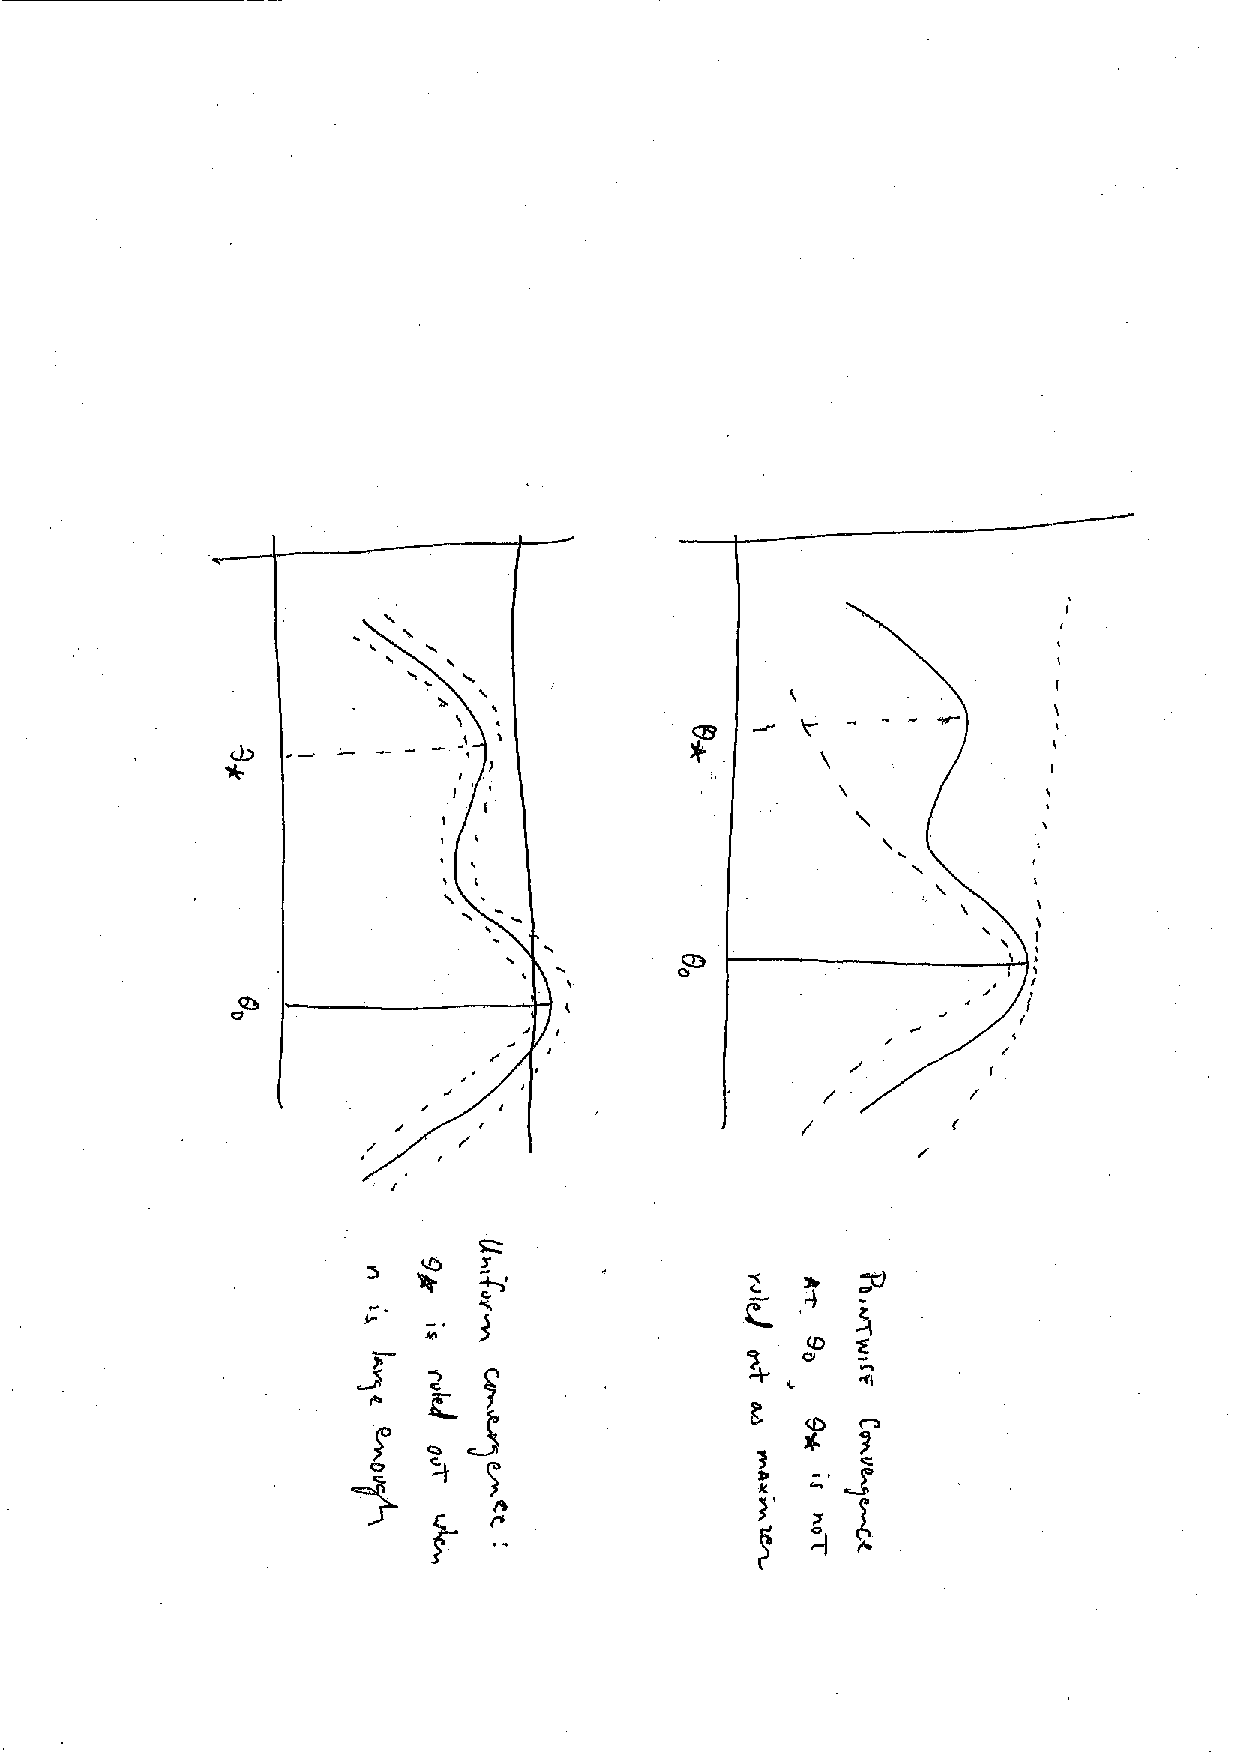
\includegraphics[angle=90,width=10cm]{Examples/Figures/UniformConvergence}

\end{figure}

\item The assumption that $\theta^{0}$ is in the interior of $\overline{\Theta}$ (part of the identification assumption) has not been used to prove consistency, so we could directly assume that $\theta^{0}$ is simply an element of a compact set $\overline{\Theta}.$ The reason that we assume it's in the interior here is that this is necessary for subsequent proof of asymptotic normality, and I'd like to maintain a minimal set of simple assumptions, for clarity. Parameters on the boundary of the parameter set cause theoretical difficulties that we will not deal with in this course. Just note that conventional hypothesis testing methods do not apply in this case. 
\item Note that $s_{n}\left(\theta\right)$ is not required to be continuous, though $s_{\infty}(\theta)$ is.
\end{itemize}
\newpage{}


\subsubsection{Sufficient conditions for assumption (b)}

We need a uniform strong law of large numbers in order to verify assumption (2) of Theorem \ref{Consistency of ee}. To verify the uniform convergence assumption, it is often feasible to employ the following set of stronger assumptions:
\begin{itemize}
\item the parameter space is compact, which is given by assumption (b)
\item the objective function $s_{n}(\theta)$ is continuous and bounded with probability one on the entire parameter space
\item a standard SLLN can be shown to apply to some point $\theta$ in the parameter space. That is, we can show that $s_{n}(\theta)\stackrel{a.s.}{\rightarrow}s_{\infty}(\theta)$ for some $\theta$. Note that in most cases, the objective function will be an average of terms, such as 
\[
s_{n}(\theta)=\frac{1}{n}\sum_{t=1}^{n}s_{t}(\theta)
\]
As long as the $s_{t}(\theta)$ are not too strongly dependent, and have finite variances, we can usually find a SLLN that will apply.
\end{itemize}
With these assumptions, it can be shown that pointwise convergence holds throughout the parameter space, so we obtain the needed uniform convergence.

These are reasonable conditions in many cases, and henceforth when dealing with specific estimators we'll simply assume that pointwise almost sure convergence can be extended to uniform almost sure convergence in this way. \newpage{}


\section{Example: \label{eeolsexample}Consistency of Least Squares}

We suppose that data is generated by random sampling of $(Y,X)$, where $y_{t}=\beta_{0}x_{t}$ $+\varepsilon_{t}$. $\left(X,\varepsilon\right)$ has the common distribution function $F_{Z}=\mu_{x}\mu_{\varepsilon}$ ($x$ and $\varepsilon$ are independent) with support $\mathcal{Z=X}\times\mathcal{E}.$ Suppose that the variances $\sigma_{X}^{2}$ and $\sigma_{\varepsilon}^{2}$ are finite. The sample objective function for a sample size $n$ is 
\begin{eqnarray*}
s_{n}(\theta) & = & 1/n\sum_{t=1}^{n}\left(y_{t}-\beta x_{t}\right)^{2}=1/n\sum_{i=1}^{n}\left(\beta_{0}x_{t}+\varepsilon_{t}-\beta x_{t}\right)^{2}\\
 & = & 1/n\sum_{t=1}^{n}\left(x_{t}\left(\beta_{0}-\beta\right)\right)^{2}+2/n\sum_{t=1}^{n}x_{t}\left(\beta_{0}-\beta\right)\varepsilon_{t}+1/n\sum_{t=1}^{n}\varepsilon_{t}^{2}
\end{eqnarray*}
 
\begin{itemize}
\item Considering the last term, by the SLLN, 
\[
1/n\sum_{t=1}^{n}\varepsilon_{t}^{2}\stackrel{a.s.}{\rightarrow}\int_{\mathcal{X}}\int_{\mathcal{E}}\varepsilon^{2}d\mu_{\mathcal{X}}d\mu_{\mathcal{E}}=\sigma_{\varepsilon}^{2}.
\]
 
\item Considering the second term, since $E(\varepsilon)=0$ and $X$ and $\varepsilon$ are independent, the SLLN implies that it converges to zero. 
\item Finally, for the first term, for a given $\beta$, we assume that a SLLN applies so that
\begin{eqnarray}
1/n\sum_{t=1}^{n}\left(x_{t}\left(\beta_{0}-\beta\right)\right)^{2} & \stackrel{a.s.}{\rightarrow} & \int_{\mathcal{X}}\left(x\left(\beta_{0}-\beta\right)\right)^{2}d\mu_{\mathcal{X}}\label{olslim}\\
 & = & \left(\beta^{0}-\beta\right)^{2}\int_{\mathcal{X}}x^{2}d\mu_{\mathcal{X}}\nonumber \\
 & = & \left(\beta^{0}-\beta\right)^{2}E\left(X^{2}\right)\nonumber 
\end{eqnarray}
 
\end{itemize}
Finally, the objective function is clearly continuous, and the parameter space is assumed to be compact, so the convergence is also uniform. Thus, 
\[
s_{\infty}(\beta)=\left(\beta^{0}-\beta\right)^{2}E\left(X^{2}\right)+\sigma_{\varepsilon}^{2}
\]
 A minimizer of this is clearly $\beta=\beta^{0}.$

\newpage{}
\begin{xca}
\label{Identification of OLS} Show that in order for the above solution to be unique it is necessary that $E(X^{2})\neq0.$ Interpret this condition.
\end{xca}
This example shows that Theorem \ref{Consistency of ee} can be used to prove strong consistency of the OLS\ estimator. There are easier ways to show this, of course - this is only an example of application of the theorem. \newpage{}

For a more concrete example, Figure \ref{fig:Consistency-of-OLS} shows computations that illustrate that the OLS estimator is consistent, when the true relationship is $y=1+1x+\epsilon,$ $\epsilon$ satisfies the classical assumptions, and $x$ is distributed uniform$(0,1).$

\begin{figure}
\caption{\label{fig:Consistency-of-OLS}Consistency of OLS}


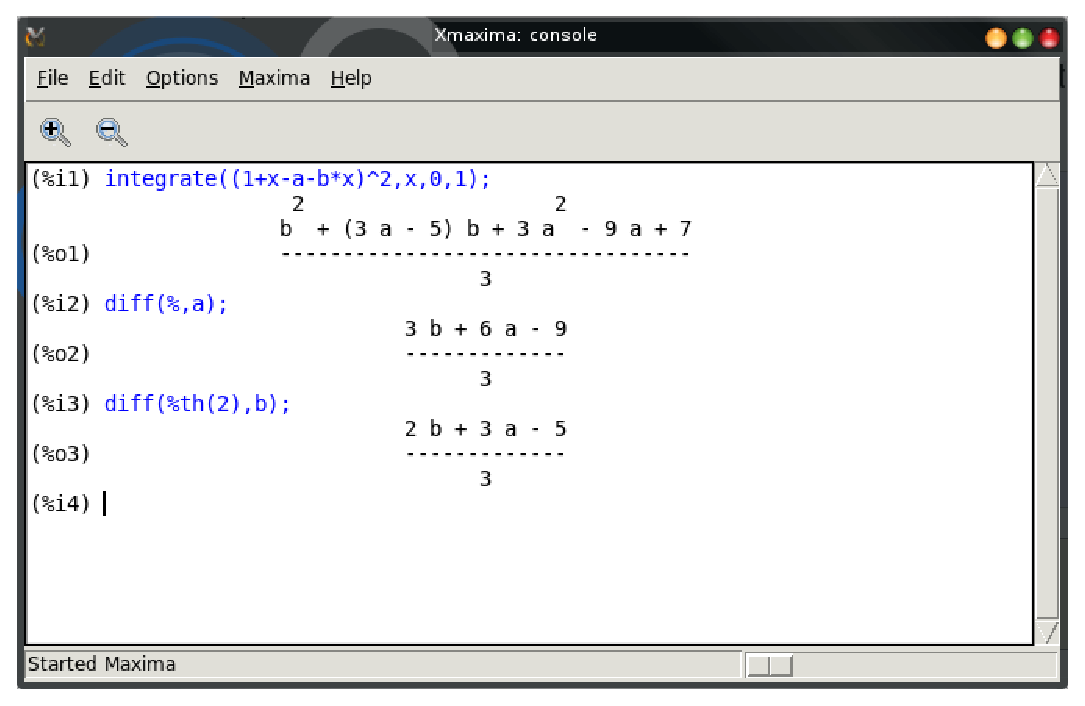
\includegraphics[width=15cm]{Examples/Figures/OLSextremum}
\end{figure}
\newpage{}


\section{More on the limiting objective function: correctly and incorrectly specified models}

The limiting objective function in assumption (b) is $s_{\infty}(\theta)$. What is the nature of this function and where does it come from?
\begin{itemize}
\item Remember our paradigm - data is presumed to be generated as a draw from $f_{Z_{n}}(z)$, and the objective function is $s_{n}(Z_{n},\theta)$.
\item Usually, $s_{n}(Z_{n},\theta)$ is an average of terms.
\item The limiting objective function is found by applying a strong (weak) law of large numbers to $s_{n}(Z_{n},\theta)$.
\item A strong (weak) LLN says that an average of terms converges almost surely (in probability) to the limit of the expectation of the average.
\end{itemize}
Supposing one holds,
\[
s_{\infty}(\theta)=\lim_{n\rightarrow\infty}\mathcal{E}s_{n}(Z_{n},\theta)=\lim_{n\rightarrow\infty}\int_{\mathcal{Z}_{n}}s_{n}(z,\theta)f_{Z_{n}}(z)dz
\]
\newpage{}Now suppose that the density $f_{Z_{n}}(z)$ that characterizes the DGP is parametric: $f_{Z_{n}}(z;\rho),\,\rho\in\varrho$, and the data is generated by $\rho^{0}\in\varrho$. Now we have two parameters to worry about, $\theta$ and $\rho$. We are probably interested in learning about the true DGP, which means that $\rho^{0}$ is the item of interest. When the DGP is parametric, the limiting objective function is 
\[
s_{\infty}(\theta)=\lim_{n\rightarrow\infty}\mathcal{E}s_{n}(Z_{n},\theta)=\lim_{n\rightarrow\infty}\int_{\mathcal{Z}_{n}}s_{n}(z,\theta)f_{Z_{n}}(z;\rho^{0})dz
\]
and we can write the limiting objective function as $s_{\infty}(\theta,\rho^{0})$ to emphasize the dependence on the parameter of the DGP. From the theorem, we know that $\hat{\theta}_{n}\stackrel{a.s.}{\rightarrow}\theta^{0}$ What is the relationship between $\theta^{0}$ and $\rho^{0}$?
\begin{itemize}
\item $\rho$ and $\theta$ may have different dimensions. Often, the statistical model (with parameter $\theta)$ only partially describes the DGP. For example, the case of OLS with errors of unknown distribution. In some cases, the dimension of $\theta$ may be greater than that of $\rho.$ For example, fitting a polynomial to an unknown nonlinear function. \newpage{}\end{itemize}
\begin{enumerate}
\item case 1: If knowledge of $\theta^{0}$ is sufficient for knowledge of $\rho^{0}$, we have a correctly and fully specified model. $\theta^{0}$ is referred to as the \emph{true parameter value}. Example \ref{eeolsexample} illustrates this case.
\item case 2: If knowledge of $\theta^{0}$ is sufficient for knowledge of some but not all elements of $\rho^{0},$ we have a correctly specified \emph{semiparametric} model. $\theta^{0}$ is referred to as the \emph{true parameter value}, understanding that not all parameters of the DGP are estimated. An example would be OLS with heteroscedasticity of unknown form: we can learn about the parameters of the conditional mean, but not about the conditional variances.
\item case 3: If knowledge of $\theta^{0}$ is not sufficient for knowledge of any elements of $\rho^{0},$ or if it causes us to draw false conclusions regarding at least some of the elements of $\rho^{0},$ our model is \emph{misspecified}. $\theta^{0}$ is referred to as the \emph{pseudo-true parameter value}. The next section provides an example.
\end{enumerate}
\newpage{}


\section{Example: Inconsistency of Misspecified Least Squares}

You already know that the OLS estimator is inconsistent when relevant variables are omitted. Let's verify this result in the context of extremum estimators. We suppose that data is generated by random sampling of $(Y,X)$, where $y_{t}=\beta_{0}x_{t}$ $+\varepsilon_{t}$. $\left(X,\varepsilon\right)$ has the common distribution function $F_{Z}=\mu_{x}\mu_{\varepsilon}$ ($x$ and $\varepsilon$ are independent) with support $\mathcal{Z=X}\times\mathcal{E}.$ Suppose that the variances $\sigma_{X}^{2}$ and $\sigma_{\varepsilon}^{2}$ are finite. However, the econometrician is unaware of the true DGP, and instead proposes the misspecified model $y_{t}=\gamma_{0}w_{t}$ $+\eta_{t}$. Suppose that $E(W\epsilon)=0$ but that $E(WX)\ne0.$

The sample objective function for a sample size $n$ is 
\begin{eqnarray*}
s_{n}(\gamma) & = & 1/n\sum_{t=1}^{n}\left(y_{t}-\gamma w_{t}\right)^{2}=1/n\sum_{i=1}^{n}\left(\beta_{0}x_{t}+\varepsilon_{t}-\gamma w_{t}\right)^{2}\\
 & = & 1/n\sum_{t=1}^{n}\left(\beta_{0}x_{t}\right)^{2}+1/n\sum_{t=1}^{n}\left(\gamma w_{t}\right)^{2}+1/n\sum_{t=1}^{n}\varepsilon_{t}^{2}\\
 &  & +2/n\sum_{t=1}^{n}\beta_{0}x_{t}\varepsilon_{t}-2/n\sum_{t=1}^{n}\beta_{0}\gamma x_{t}w_{t}-2/n\sum_{t=1}^{n}\varepsilon_{t}x_{t}w_{t}
\end{eqnarray*}
 Using arguments similar to above, 
\[
s_{\infty}(\gamma)=\gamma^{2}E\left(W^{2}\right)-2\beta_{0}\gamma E(WX)+C
\]
 So, $\gamma_{0}=\frac{\beta_{0}E(WX)}{E(W^{2})}$, which is the true parameter of the DGP, multiplied by the pseudo-true value of a regression of $X$ on $W.$ The OLS estimator is not consistent for the true parameter, $\beta_{0}$ 


\subsubsection{Summary}

The theorem for consistency is really quite intuitive. It says that, with probability one, an extremum estimator converges to the value that maximizes the limit of the expectation of the objective function. Because the objective function may or may not make sense, depending on how good or poor is the model, we may or may not be estimating parameters of the DGP.\newpage{}


\section{Example: Linearization of a nonlinear model}

Ref. Gourieroux and Monfort, section 8.3.4. White, \emph{Intn'l Econ. Rev.} 1980 is an earlier reference.

Suppose we have a nonlinear model 
\[
y_{i}=h(x_{i},\theta^{0})+\varepsilon_{i}
\]
 where 
\[
\varepsilon_{i}\sim iid(0,\sigma^{2})
\]
 The \emph{nonlinear least squares} estimator solves 
\[
\hat{\theta}_{n}=\arg\min\frac{1}{n}\sum_{i=1}^{n}\left(y_{i}-h(x_{i},\theta)\right)^{2}
\]
 \newpage{}We'll study this more later, but for now it is clear that the foc for minimization will require solving a set of nonlinear equations. A common approach to the problem seeks to avoid this difficulty by \emph{linearizing} the model. A first order Taylor's series expansion about the point $x_{0}$ with remainder gives 
\[
y_{i}=h(x^{0},\theta^{0})+\left(x_{i}-x_{0}\right)^{\prime}\frac{\partial h(x_{0},\theta^{0})}{\partial x}+\nu_{i}
\]
 where $\nu_{i}$ encompasses both $\varepsilon_{i}$ and the Taylor's series remainder. Note that $\nu_{i}$ is no longer a classical error - its mean is not zero. We should expect problems.

Define 
\begin{eqnarray*}
\alpha^{*} & = & h(x_{0},\theta^{0})-x_{0}^{\prime}\frac{\partial h(x^{0},\theta^{0})}{\partial x}\\
\beta^{*} & = & \frac{\partial h(x_{0},\theta^{0})}{\partial x}
\end{eqnarray*}
 

Given this, one might try to estimate $\alpha^{*}$ and $\beta^{*}$ by applying OLS to 
\[
y_{i}=\alpha+\beta x_{i}+\nu_{i}
\]
\newpage{}
\begin{itemize}
\item Question, will $\hat{\alpha}$ and $\hat{\beta}$ be consistent for $\alpha^{*}$ and $\beta^{*}$?
\item The answer is no, as one can see by interpreting $\hat{\alpha}$ and $\hat{\beta}$ as extremum estimators. Let $\gamma=(\alpha,\beta^{\prime})^{\prime}.$
\end{itemize}
\[
\hat{\gamma}=\arg\min s_{n}(\gamma)=\frac{1}{n}\sum_{i=1}^{n}\left(y_{i}-\alpha-\beta x_{i}\right)^{2}
\]
 The objective function converges to its expectation 
\[
s_{n}(\gamma)\stackrel{u.a.s.}{\rightarrow}s_{\infty}(\gamma)=\mathcal{E}_{X}\mathcal{E}_{Y|X}\left(y-\alpha-\beta x\right)^{2}
\]
 and $\hat{\gamma}$ converges $a.s.$ to the $\gamma^{0}$ that minimizes $s_{\infty}(\gamma)$: 
\[
\gamma^{0}=\arg\min\mathcal{E}_{X}\mathcal{E}_{Y|X}\left(y-\alpha-\beta x\right)^{2}
\]
 Noting that 
\begin{eqnarray*}
\mathcal{E}_{X}\mathcal{E}_{Y|X}\left(y-\alpha-x^{\prime}\beta\right)^{2} & = & \mathcal{E}_{X}\mathcal{E}_{Y|X}\left(h(x,\theta^{0})+\varepsilon-\alpha-\beta x\right)^{2}\\
 & = & \sigma^{2}+\mathcal{E}_{X}\left(h(x,\theta^{0})-\alpha-\beta x\right)^{2}
\end{eqnarray*}
 since cross products involving $\varepsilon$ drop out. $\alpha^{0}$ and $\beta^{0}$ correspond to the hyperplane that is closest to the true regression function $h(x,\theta^{0})$ according to the mean squared error criterion. This depends on both the shape of $h(\cdot)$ and the density function of the conditioning variables. See Figure \ref{fig:Linear-Approximation}. \newpage{}

\begin{figure}


\caption{\label{fig:Linear-Approximation}Linear Approximation}


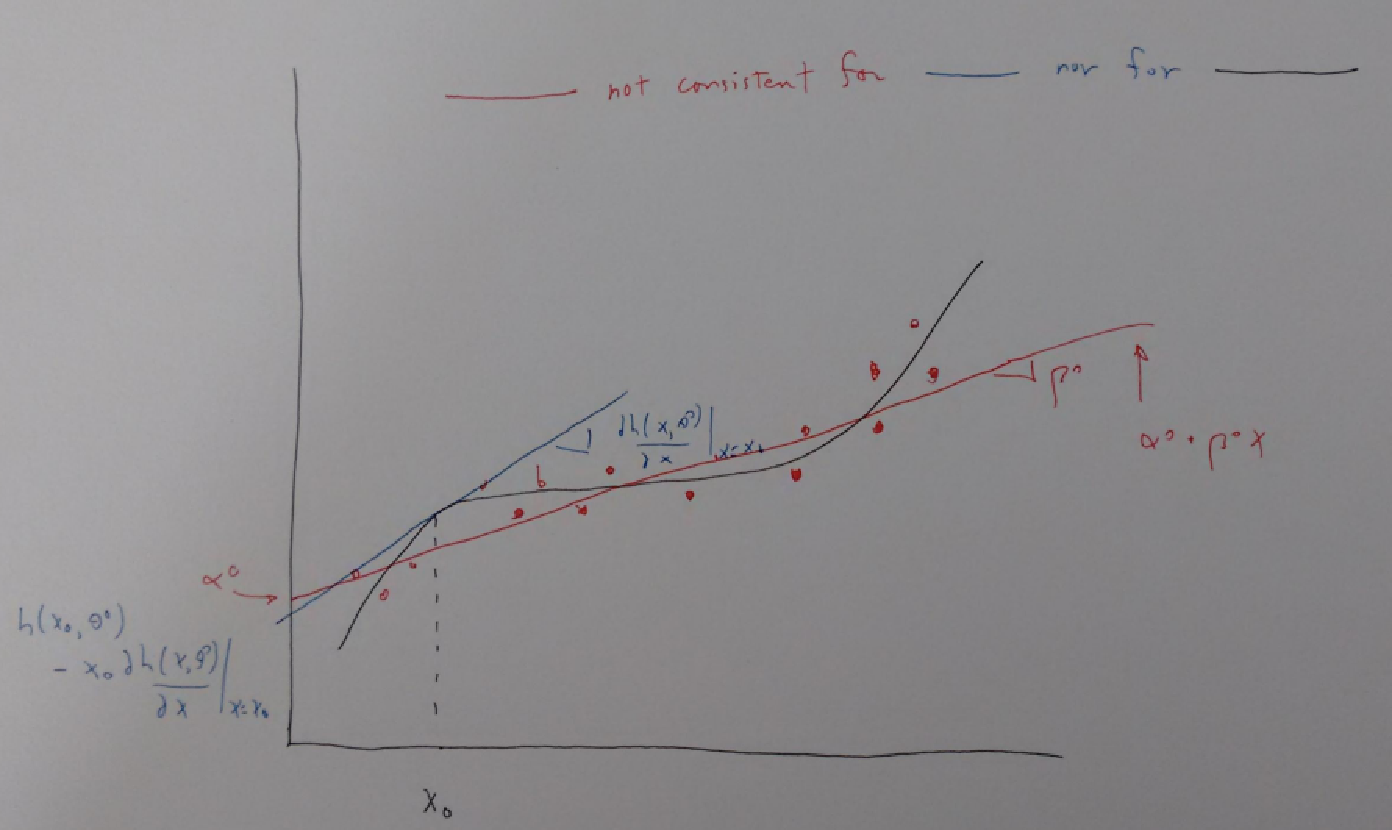
\includegraphics[width=12cm]{Examples/Figures/LinearApproximation}

\end{figure}
\newpage{}
\begin{itemize}
\item It is clear that the tangent line does not minimize MSE, since, for example, if $h(x,\theta^{0})$ is concave, all errors between the tangent line and the true function are negative.
\item Note that the true underlying parameter $\theta^{0}$ is not estimated consistently, either (it may be of a different dimension than the dimension of the parameter of the approximating model, which is 2 in this example).
\item see Exercise \ref{ols} in the list at the end of the chapter for a practical example.
\item Second order and higher-order approximations suffer from exactly the same problem, though to a less severe degree, of course. For this reason, translog, Generalized Leontiev and other ``flexible functional forms'' based upon second-order approximations in general suffer from bias and inconsistency. The bias may not be too important for analysis of conditional means, but it can be very important for analyzing first and second derivatives. In production and consumer analysis, first and second derivatives (\emph{e.g.,} elasticities of substitution) are often of interest, so in this case, one should be cautious of unthinking application of models that impose stong restrictions on second derivatives.
\item This sort of linearization about a long run equilibrium is a common practice in working with dynamic macroeconomic models. It is justified for the purposes of theoretical analysis of a model \emph{given} the model's parameters, but it will lead to\emph{ bias and inconsistency} if it is done before estimation of the parameters of the model using data. The section on simulation-based methods offers a means of obtaining consistent estimators of the parameters of dynamic macro models that are too complex for standard methods of analysis. 
\end{itemize}
\newpage{}


\section{Asymptotic Normality}

A consistent estimator is oftentimes not very useful unless we know how fast it is likely to be converging to the true value, and the probability that it is far away from the true value. Establishment of asymptotic normality with a known scaling factor solves these two problems. The following theorem is similar to Amemiya's Theorem 4.1.3 (pg. 111).
\begin{thm}
\emph{{[}Asymptotic normality of e.e.{]}} \label{Normality of ee}In addition to the assumptions of Theorem \ref{Consistency of ee}, assume

(a) $\mathcal{J}_{n}(\theta)\equiv D_{\theta}^{2}s_{n}(\theta)$ exists and is continuous in an open, convex neighborhood of $\theta^{0}.$

(b) $\{\mathcal{J}_{n}(\theta_{n})\}\stackrel{a.s.}{\rightarrow}\mathcal{J}_{\infty}(\theta^{0}),$ a finite negative definite matrix, for any sequence $\{\theta_{n}\}$ that converges almost surely to $\theta^{0}.$

(c) $\sqrt{n}D_{\theta}s_{n}(\theta^{0})\stackrel{d}{\rightarrow}N\left[0,\mathcal{I}_{\infty}(\theta^{0})\right],$ where $\mathcal{I}_{\infty}(\theta^{0})=\lim_{n\rightarrow\infty}Var\sqrt{n}D_{\theta}s_{n}(\theta^{0})$

Then $\sqrt{n}\left(\hat{\theta}-\theta^{0}\right)\stackrel{d}{\rightarrow}N\left[0,\mathcal{J}_{\infty}(\theta^{0})^{-1}\mathcal{I}_{\infty}(\theta^{0})\mathcal{J}_{\infty}(\theta^{0})^{-1}\right]$
\end{thm}
\newpage{}\textbf{Proof:} By Taylor expansion: 
\[
D_{\theta}s_{n}(\hat{\theta}_{n})=D_{\theta}s_{n}(\theta^{0})+D_{\theta}^{2}s_{n}(\theta^{*})\left(\hat{\theta}-\theta^{0}\right)
\]
 where $\theta^{*}=\lambda\hat{\theta}+(1-\lambda)\theta^{0},$ $0\leq\lambda\leq1.$
\begin{itemize}
\item Note that $\hat{\theta}$ will be in the neighborhood where $D_{\theta}^{2}s_{n}(\theta)$ exists with probability one as $n$ becomes large, by consistency.
\item Now the l.h.s. of this equation is zero, at least asymptotically, since $\hat{\theta}_{n}$ is a maximizer and the f.o.c. must hold exactly since the limiting objective function is strictly concave in a neighborhood of $\theta^{0}.$
\item Also, since $\theta^{*}$ is between $\hat{\theta}_{n}$ and $\theta^{0},$ and since $\hat{\theta}_{n}$ $\stackrel{a.s.}{\rightarrow}$ $\theta^{0}$ , assumption (b) gives 
\[
D_{\theta}^{2}s_{n}(\theta^{*})\stackrel{a.s.}{\rightarrow}\mathcal{J}_{\infty}(\theta^{0})
\]

\end{itemize}
So 
\[
0=D_{\theta}s_{n}(\theta^{0})+\left[\mathcal{J}_{\infty}(\theta^{0})+o_{s}(1)\right]\left(\hat{\theta}-\theta^{0}\right)
\]


And 
\[
0=\sqrt{n}D_{\theta}s_{n}(\theta^{0})+\left[\mathcal{J}_{\infty}(\theta^{0})+o_{s}(1)\right]\sqrt{n}\left(\hat{\theta}-\theta^{0}\right)
\]
 Now $\sqrt{n}D_{\theta}s_{n}(\theta^{0})\stackrel{d}{\rightarrow}N\left[0,\mathcal{I}_{\infty}(\theta^{0})\right]$ by assumption c, so 
\[
-\left[\mathcal{J}_{\infty}(\theta^{0})+o_{s}(1)\right]\sqrt{n}\left(\hat{\theta}-\theta^{0}\right)\stackrel{d}{\rightarrow}N\left[0,\mathcal{I}_{\infty}(\theta^{0})\right]
\]
 Also, $\left[\mathcal{J}_{\infty}(\theta^{0})+o_{s}(1)\right]\stackrel{a.s.}{\rightarrow}\mathcal{J}(\theta^{0}),$ so 
\[
\sqrt{n}\left(\hat{\theta}-\theta^{0}\right)\stackrel{d}{\rightarrow}N\left[0,\mathcal{J}_{\infty}(\theta^{0})^{-1}\mathcal{I}_{\infty}(\theta^{0})\mathcal{J}_{\infty}(\theta^{0})^{-1}\right]
\]
by the Slutsky Theorem (see Gallant, Theorem 4.6).\newpage{}

Figure \ref{fig:Effects-of-} shows the effects of the two components, the variability of the gradient, and the slope of the gradient. 
\begin{figure}


\caption{\label{fig:Effects-of-}Effects of $I_{\mbox{\ensuremath{\infty}}}$ and $J_{\infty}$}


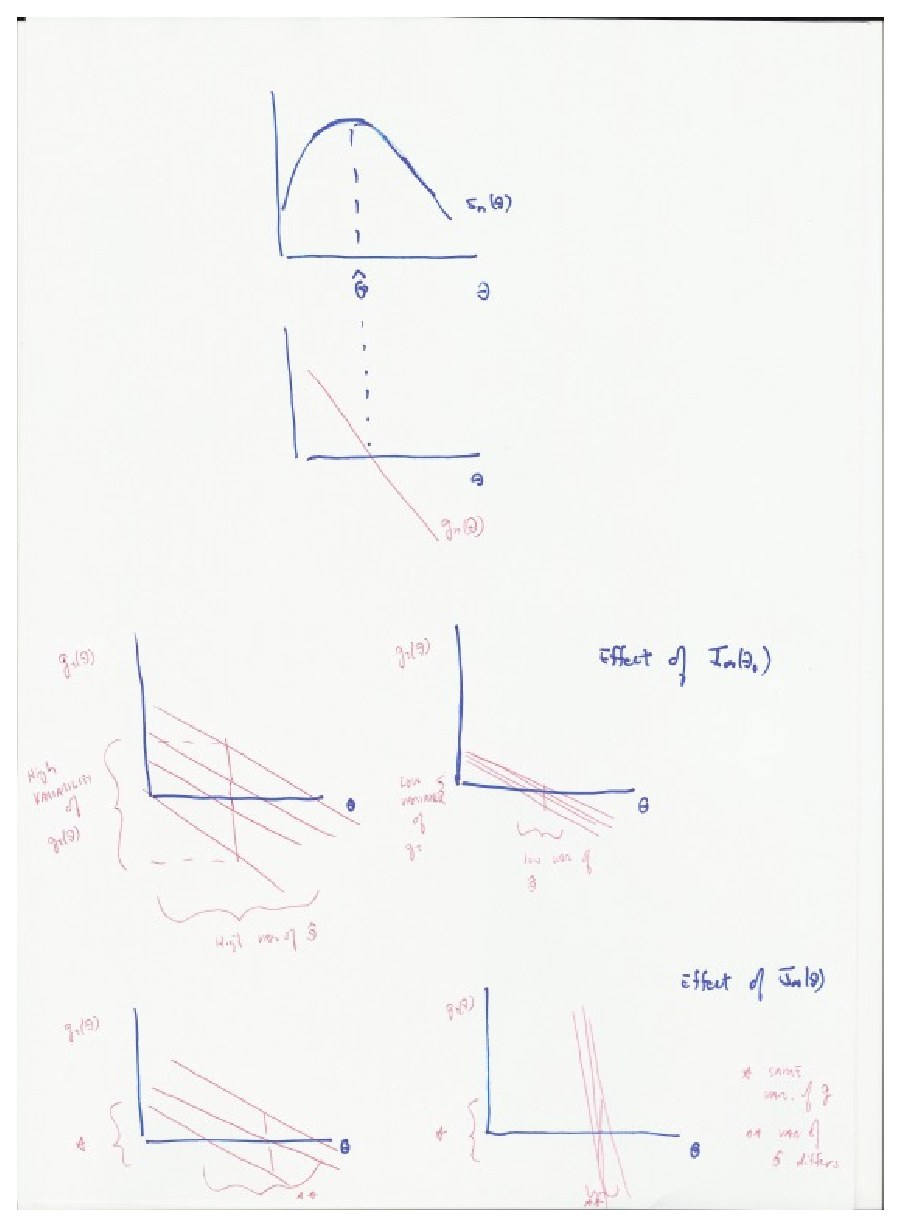
\includegraphics[height=0.65\paperwidth]{Examples/Figures/IJ}

\end{figure}

\begin{itemize}
\item \textbf{Skip this in lecture.} A note on the order of these matrices: Supposing that $s_{n}(\theta)$ is representable as an average of $n$ terms, which is the case for all estimators we consider, $D_{\theta}^{2}s_{n}(\theta)$ is also an average of $n$ matrices, the elements of which are not centered (they do not have zero expectation). Supposing a SLLN applies, the almost sure limit of $D_{\theta}^{2}s_{n}(\theta^{0}),$ $\mathcal{J}_{\infty}(\theta^{0})=O(1),$ as we saw in Example \ref{uncentered}. On the other hand, assumption (c):$\sqrt{n}D_{\theta}s_{n}(\theta^{0})\stackrel{d}{\rightarrow}N\left[0,\mathcal{I}_{\infty}(\theta^{0})\right]$ means that 
\[
\sqrt{n}D_{\theta}s_{n}(\theta^{0})=\mathnormal{O_{p}(1)}
\]
 where we use the result of Example \ref{normop1}. If we were to omit the $\sqrt{n},$ we'd have 
\begin{eqnarray*}
D_{\theta}s_{n}(\theta^{0}) & = & n^{-\frac{1}{2}}O_{p}(1)\\
 & = & O_{p}\left(n^{-\frac{1}{2}}\right)
\end{eqnarray*}
 where we use the fact that $O_{p}(n^{r})O_{p}(n^{q})=O_{p}(n^{r+q}).$ The sequence $D_{\theta}s_{n}(\theta^{0})$ \emph{is} centered, so we need to scale by $\sqrt{n}$ to avoid convergence to zero.\newpage{}
\end{itemize}

\section{Example: Classical linear model}

Let's use the results to get the asymptotic distribution of the OLS estimator applied to the classical model, to verify that we obtain the results seen before. The OLS criterion is

\begin{eqnarray*}
s_{n}(\beta) & = & \frac{1}{n}\left(y-X\beta\right)^{\prime}\left(y-X\beta\right)\\
 & = & \frac{1}{n}\left(X\beta^{0}+\epsilon-X\beta\right)^{\prime}\left(X\beta^{0}+\epsilon-X\beta\right)\\
 & = & \frac{1}{n}\left(X(\beta^{0}-\beta)+\epsilon\right)^{\prime}\left(X(\beta^{0}-\beta)+\epsilon\right)\\
 & = & \frac{1}{n}\left[\left(\beta^{0}-\beta\right)^{\prime}X^{\prime}X\left(\beta^{0}-\beta\right)+2\epsilon^{\prime}X(\beta_{0}-\beta)+\epsilon^{\prime}\epsilon\right]
\end{eqnarray*}
The first derivative is

\[
D_{\beta}s_{n}(\beta)=\frac{1}{n}\left[-2X^{\prime}X\left(\beta^{0}-\beta\right)-2X^{\prime}\epsilon\right]
\]
so, evaluating at $\beta^{0},$
\[
D_{\beta}s_{n}(\beta^{0})=-2\frac{X^{\prime}\epsilon}{n}
\]

\begin{itemize}
\item note that this is an average of terms, each of which has expectation zero: $-2\frac{X^{\prime}\epsilon}{n}=-2\frac{1}{n}\sum_{t}x_{t}\epsilon_{t}$
\item thus, a LLN tells us this converges almost surely to 0.
\item to keep this from happening, we can multiply by something that is converging to infinity. It turns out that $\sqrt{n}$ is the right choice, because then the asymptotic distribution will be stable, and a CLT will apply.
\end{itemize}
Considering $\sqrt{n}D_{\beta}s_{n}(\beta^{0})$, it has expectation 0, so the variance is the expectation of the outer product:
\begin{eqnarray*}
Var\sqrt{n}D_{\beta}s_{n}(\beta^{0}) & = & E\left[\left(-\sqrt{n}2\frac{X^{\prime}\epsilon}{n}\right)\left(-\sqrt{n}2\frac{X^{\prime}\epsilon}{n}\right)^{\prime}\right]\\
 & = & E4\frac{X^{\prime}\epsilon\epsilon^{\prime}X}{n}\\
 & = & 4\sigma_{\epsilon}^{2}E\left(\frac{X^{\prime}X}{n}\right)
\end{eqnarray*}
(assuming regressors independent of errors). Therefore
\begin{eqnarray*}
\mathcal{I}_{\infty}(\beta^{0}) & = & \lim_{n\rightarrow\infty}Var\sqrt{n}D_{\beta}s_{n}(\beta^{0})\\
 & = & 4\sigma_{\epsilon}^{2}Q_{X}
\end{eqnarray*}
where $Q_{X}=limE\left(\frac{X^{\prime}X}{n}\right),$ a finite p.d. matrix, is obtained using a LLN. 

The second derivative is
\[
\mathcal{J}_{n}(\beta)=D_{\beta}^{2}s_{n}(\beta^{0})=\frac{1}{n}\left[2X^{\prime}X\right].
\]
A SLLN tells us that this converges almost surely to the limit of its expectation:
\[
\mathcal{J}_{\infty}(\beta^{0})=2Q_{X}
\]
There's no parameter in that last expression, so uniformity is not an issue.

The asymptotic normality theorem (\ref{Normality of ee}) tells us that
\begin{eqnarray*}
\sqrt{n}\left(\hat{\beta}-\beta^{0}\right) & \stackrel{d}{\rightarrow} & N\left[0,\mathcal{J}_{\infty}(\beta^{0})^{-1}\mathcal{I}_{\infty}(\beta^{0})\mathcal{J}_{\infty}(\beta^{0})^{-1}\right]
\end{eqnarray*}
which is, given the above,
\[
\sqrt{n}\left(\hat{\beta}-\beta^{0}\right)\stackrel{d}{\rightarrow}N\left[0,\left(\frac{Q_{X}^{-1}}{2}\right)\left(4\sigma_{\epsilon}^{2}Q_{X}\right)\left(\frac{Q_{X}^{-1}}{2}\right)\right]
\]
or
\[
\sqrt{n}\left(\hat{\beta}-\beta^{0}\right)\stackrel{d}{\rightarrow}N\left[0,Q_{X}^{-1}\sigma_{\epsilon}^{2}\right].
\]
This is the same thing we saw in equation \ref{eq:asymp normality OLS}, of course. So, the theory seems to work :-)

\newpage{}


\section{Exercises}
\begin{enumerate}
\item \label{ols}Suppose that $x_{i}\sim$ uniform(0,1), and $y_{i}=1-x_{i}^{2}+\varepsilon_{i},$ where $\varepsilon_{i}$ is iid(0,$\sigma^{2}).$ Suppose we estimate the misspecified model $y_{i}=\alpha+\beta x_{i}+\eta_{i}$ by OLS. Find the numeric values of $\alpha^{0}$ and $\beta^{0}$ that are the probability limits of $\hat{\alpha}$ and $\hat{\beta}$. Hint: the correct answers are 7/6 and -1. To get some help with this exercise, you can use a computer algebra program, as was done in Figure \ref{fig:Consistency-of-OLS}. A small modification of that code would solve this problem.
\item Verify your results using Octave by generating data that follows the above model, and calculating the OLS estimator. When the sample size is very large the estimator should be very close to the analytical results you obtained in question \ref{ols}.
\item Use the asymptotic normality theorem to find the asymptotic distribution of the ML estimator of $\beta^{0}$ for the model $y=x\beta^{0}+\varepsilon,$ where $\varepsilon\sim N(0,1)$ and is independent of $x.$ This means finding $\frac{\partial^{2}}{\partial\beta\partial\beta^{\prime}}s_{n}(\beta)$, $\mathcal{J}(\beta^{0}),\left.\frac{\partial s_{n}(\beta)}{\partial\beta}\right|,$ and $\mathcal{I}(\beta^{0}).$ The expressions may involve the unspecified density of $x.$
\end{enumerate}
\newpage{}


\chapter{Maximum likelihood estimation}

Cameron and Trivedi, Ch. 5

The maximum likelihood estimator is important because it uses all of the information in a fully specified statistical model. Its use of all of the information causes it to have a number of attractive properties, foremost of which is asymptotic efficiency. For this reason, the ML estimator can serve as a benchmark against which other estimators may be measured. The ML estimator requires that the statistical model be fully specified, which essentially means that there is enough information to draw data from the DGP, given the parameter. This is a fairly strong requirement, and for this reason we need to be concerned about the possible misspecification of the statistical model. If this is the case, the ML estimator will not have the nice properties that it has under correct specification.\newpage{}


\section{The likelihood function}

Suppose we have a sample of size $n$ of the random vectors $y$ and $z$. Suppose the joint density of $Y=\left(\begin{array}{ccc}
y_{1} & \ldots & y_{n}\end{array}\right)$ and $Z=\left(\begin{array}{ccc}
z_{1} & \ldots & z_{n}\end{array}\right)$ is characterized by a parameter vector $\psi_{0}:$
\[
f_{YZ}(Y,Z,\psi_{0}).
\]
 This is the joint density of the sample. The \emph{likelihood\index{likelihood function} function} is just this density evaluated at other values $\psi$
\[
L(Y,Z,\psi)=f(Y,Z,\psi),\psi\in\Psi,
\]
 where $\Psi$ is a \emph{parameter\index{parameter space} space.}

The \emph{maximum likelihood estimator} of $\psi_{0}$ is the value of $\psi$ that maximizes the likelihood function.\newpage{}
\begin{example}
Count data. Suppose we have a sample $Y=\{y_{1},...,y_{n}\}$ where the data are counts: the number of times some event occurs in a given interval of time, e.g., number of visits to the doctor in a year. The simplest count data density is the Poisson:
\[
f_{Y}(y;\lambda)=\frac{e^{-\lambda}\lambda^{y}}{y!}
\]
If the observations are i.i.d. distributed according to this density, then the joint density of the sample is
\[
L(\lambda)=\prod_{i=1}^{n}\frac{e^{-\lambda}\lambda^{y_{i}}}{y_{i}!}=\frac{e^{-n\lambda}\lambda^{\sum y_{i}}}{\prod_{i}y_{i}!}
\]
A little algebra shows us that the value that maximizes this is $\hat{\lambda}=\bar{y}$.\end{example}
\begin{itemize}
\item we can compute the ML estimator without much trouble, and we have asymptotic theory that will allow us to test hypotheses about $\lambda$.
\item however, now suppose that each observation has its own $\lambda_{i}=\exp(x_{i}^{\prime}\beta)$ which depends on conditioning variables and a new parameter vector. We can now write the likelihood function in terms of $\beta$. 

\begin{itemize}
\item The problem is, we can't find an analytic solution for the ML estimator of $\beta.$
\item Even if we could, $\hat{\beta}$ which solves the f.o.c. is a nonlinear function of the data. How could we test hypotheses?
\item To solve these two problems, we need the methods from Ch. 11 and the theory from Ch. 12.
\end{itemize}
\end{itemize}
\newpage{}


\subsection{Exogenous variables}

The likelihood function can be factored as 
\[
f_{YZ}(Y,Z,\psi)=f_{Y|Z}(Y|Z,\theta)f_{Z}(Z,\rho)
\]
where $\theta$ are whatever elements of $\psi$ that happen to enter in the conditional density, and $\rho$ are the elements that enter into the marginal density.

Note that if $\theta$ and $\rho$ share no elements, then the maximizer of the conditional likelihood function $f_{Y|Z}(Y|Z,\theta)$ with respect to $\theta$ is the same as the maximizer of the overall likelihood function $f_{YZ}(Y,Z,\psi)=f_{Y|Z}(Y|Z,\theta)f_{Z}(Z,\rho)$, for the elements of $\psi$ that correspond to $\theta$. In this case, the variables $Z$ are said to be \emph{exogenous} for estimation of $\theta$, and we may more conveniently work with the conditional likelihood function $f_{Y|Z}(Y|Z,\theta)$ for the purposes of estimating $\theta_{0}$. Exogeneity may or may not hold, but when it does, we can simplify the problem.

With exogeneity of $Z$, the maximum likelihood estimator of $\theta_{0}$ will be $\arg\max f_{Y|Z}(Y|Z,\theta)$. We'll suppose this framework holds in what follows. If it didn't, for some variables in $Z,$ then just move those variables from $Z$ to $Y,$ until it does hold.\newpage{}


\subsection{A convenient factorization of the likelihood function}
\begin{itemize}
\item If the $n$ observations are independent, the likelihood function can be written as 
\[
L(Y|Z,\theta)=\prod_{t=1}^{n}f(y_{t}|z_{t},\theta)
\]
 
\item If this is not possible, we can always factor the likelihood into \emph{contributions of observations,} by using the fact that a joint density can be factored into the product of a marginal and conditional.
\item Then
\[
\begin{array}{c}
\underbrace{f(y_{1,}y_{2},\ldots y_{n-1},y_{n}|Z,\theta)}\\
\mathrm{joint}
\end{array}=\begin{array}{c}
\underbrace{f(y_{n}|y_{1,}y_{2},\ldots y_{n-1},Z,\theta)}\\
\mathrm{conditional}
\end{array}\begin{array}{c}
\underbrace{f(y_{1,}y_{2},\ldots y_{n-1}|Z,\theta)}\\
\mathrm{marginal}
\end{array}
\]

\item do the same thing for $y_{n-1}$ in the last term, and keep iterating. \newpage{}
\item Then, in the end, we have
\end{itemize}
\[
L(Y,\theta)=f(y_{n}|y_{1,}y_{2},\ldots y_{t-n},Z,\theta)f(y_{n-1}|y_{1,}y_{2},\ldots y_{n-2},Z,\theta)\cdots f(y_{2}|y_{1},Z,\theta)f(y_{1}|Z,\theta)
\]


To simplify notation, define 
\begin{eqnarray*}
x_{t} & = & \{y_{1},y_{2},...,y_{t-1},Z\}
\end{eqnarray*}

\begin{itemize}
\item Usually, for time series data, conditional densities depend only on current period exogenous variables, as the effects of lagged exogenous variables are transmitted though the realizations of the lagged endogenous variables, and economic models normally don't involve leads of exogenous variables. If this is the case, $x_{1}=z_{1},$ $x_{2}=\{y_{1},z_{2}\}$, \emph{etc}. - it contains exogenous and predetermined endogenous variables. 
\item Regardless of the specific contents of $x_{t},$ the likelihood function can now be written as 
\[
L(Y|X;\theta)=\prod_{t=1}^{n}f(y_{t}|x_{t},\theta)
\]
\newpage{}The criterion function can be defined as the average log-likelihood function: 
\[
s_{n}(\theta)=\frac{1}{n}\ln L(Y|X;\theta)=\frac{1}{n}\sum_{t=1}^{n}\ln f(y_{t}|x_{t};\theta)
\]
 The maximum likelihood estimator may thus be defined equivalently as 
\[
\hat{\theta}=\arg\max s_{n}(\theta),
\]
 where the set maximized over is defined below. Since $\ln(\cdot)$ is a monotonic increasing function, $\ln L$ and $L$ maximize at the same value of $\theta.$ Dividing by $n$ has no effect on $\hat{\theta}.$\newpage{}\end{itemize}
\begin{example}
Example: \label{sub:Example:-Bernoulli-trial}Bernoulli trial\\
Suppose that we are flipping a coin that may be biased, so that the probability of a heads may not be 0.5. Maybe we're interested in estimating the probability of a heads. Let $Y=1(heads)$ be a binary variable that indicates whether or not a heads is observed. The outcome of a toss is a Bernoulli random variable:
\begin{eqnarray*}
f_{Y}(y,p_{0}) & = & p_{0}^{y}\left(1-p_{0}\right)^{1-y},y\in\{0,1\}\\
 & = & 0,y\notin\{0,1\}
\end{eqnarray*}
So a representative term that enters the likelihood function is
\[
f_{Y}(y,p)=p^{y}\left(1-p\right)^{1-y}
\]
and
\[
\ln f_{Y}(y,p)=y\ln p+\left(1-y\right)\ln\left(1-p\right)
\]
For this example, the average log-likelihood function is $s_{n}(p)=\frac{1}{n}\sum_{t=1}^{n}y_{t}\ln p+\left(1-y_{t}\right)\ln\left(1-p\right)$.

The derivative of a representative term is
\begin{eqnarray*}
\frac{\partial\ln f_{Y}(y,p)}{\partial p} & = & \frac{y}{p}-\frac{\left(1-y\right)}{\left(1-p\right)}\\
 & = & \frac{y-p}{p\left(1-p\right)}
\end{eqnarray*}
so, averaging this over a sample of size $n$, the gradient is
\[
\frac{\partial s_{n}(p)}{\partial p}=\frac{1}{n}\sum_{t=1}^{n}\frac{y_{t}-p}{p\left(1-p\right)}.
\]
Setting to zero and solving gives
\begin{equation}
\hat{p}=\bar{y}\label{eq:mle Bernoulli}
\end{equation}
So it's easy to calculate the MLE of $p_{0}$ in this case. \end{example}
\begin{itemize}
\item We also know that the sample mean converges to the true mean, from basic statistics. 
\item The mean is $E(Y)=\sum_{y=0}^{y=1}yp_{0}^{y}\left(1-p_{0}\right)^{1-y}=p_{0}$. 
\item Thus, the ML is consistent. 
\item For future reference, note that $Var(Y)=E(Y^{2})-\left[E(Y)\right]^{2}=p_{0}-p_{0}^{2}$.
\end{itemize}
We see that the ML estimator is consistent, for this model. However, let's verify that the consistency theorem for extremum estimators gives us the same result:
\begin{itemize}
\item A LLN tells us that, for a given $p,$ $s_{n}(p)\rightarrow^{a.s.}p_{0}\ln p+(1-p_{0})\ln(1-p)$. 
\item The parameter space must be compact. We know that $p_{0}$ lies between 0 and 1, so this helps set the parameter space.
\item the objective function is obviously continuous in the parameter
\item we need the objective function to be bounded, for the simple sufficient conditions for the consistency theorem to hold. So, we need to assume that $p$ can't go to 0 or to 1. This means that the parameter space must be a compact subset of $\left(0,1\right)$.
\item With these conditions, the a.s. convergence is also uniform. 
\item The consistency theorem for extremum estimators tells us that the ML estimator converges to the value that maximizes the limiting objective function. Because $s_{\infty}(p)=p_{0}\ln p+(1-p_{0})\ln(1-p)$, we can easily check that the maximizer is $p_{0}$. 
\item So, the ML estimator is consistent for the true probability.
\end{itemize}
\newpage{}
\begin{example}
\emph{\label{exa:Likelihood-function-of}Likelihood function and MLE of classical linear regression model}. Let's supp�se that a dependent variable is normally distributed:$y\sim N(\mu_{0},\sigma_{0}^{2})$, so
\[
f_{y}(y;\mu_{0},\sigma_{0}^{2})=\frac{1}{\sqrt{2\pi\sigma_{0}^{2}}}\exp\left(-\frac{(y-\mu_{0})^{2}}{2\sigma_{0}^{2}}\right)
\]
Suppose that the mean, $\mu_{0}$, depends on some regressors, $x$. The simplest way to do this is to assume that $\mu_{0}=x^{\prime}\beta_{0}.$ With this, the density, conditional on $x$ is 
\[
f_{y}(y|x;\beta_{0},\sigma_{0}^{2})=\frac{1}{\sqrt{2\pi\sigma_{0}^{2}}}\exp\left(-\frac{(y-x^{\prime}\beta_{0})^{2}}{2\sigma_{0}^{2}}\right)
\]
This is an example of \emph{parameterization }of a density, making some parameters depend on additional variables and new parameters. With an i.i.d. sample of size $n$, the overall conditional density is the product of the conditional density of each observation: 
\[
f_{y}(y_{1},y_{2},...,y_{n}|x_{1},x_{2},...,x;\beta_{0},\sigma_{0}^{2})=\prod_{t=1}^{n}\frac{1}{\sqrt{2\pi\sigma_{0}^{2}}}\exp\left(-\frac{(y_{t}-x_{t}^{\prime}\beta_{0})^{2}}{2\sigma_{0}^{2}}\right)
\]
\newpage{}Taking logarithms, and evaluating at some point in the parameter space, we get the log-likelihood function: 
\[
\ln L(Y|X;\beta,\sigma^{2})=-n\ln\sqrt{2\pi}-n\ln\sigma-\sum_{t=1}^{n}\frac{\left(y_{t}-x_{t}'\beta\right)^{2}}{2\sigma^{2}}
\]
\end{example}
\begin{itemize}
\item Observe that the first order conditions for $\beta$ are the same as for the OLS estimator. We know that the OLS estimator is consistent without making distributional assumptions regarding the errors. As long as the assumptions for consistency of OLS hold (fundamentally, weak exogeneity), then this estimator will be consistent for $\beta$ as well, even if the normality assumption is not correct. This would be an example of \emph{quasi-maximum likelihood} estimation: ''ML'' estimation of a misspecified model. Sometimes the QML estimator is consistent, sometimes it's not.
\item A Octave/Matlab example that shows how to compute the maximum likelihood estimator for data that follows the CLRM with normality is in  \htmladdnormallink{NormalExample.m}{file:///home/michael/Mystuff/Econometrics/Examples/MLE/NormalExample.m} , which makes use of  \htmladdnormallink{NormalLF.m}{file:///home/michael/Mystuff/Econometrics/Examples/MLE/NormalLF.m} .\newpage{}
\end{itemize}

\section{Consistency of MLE}

The MLE is an extremum estimator, given basic assumptions it is consistent for the value that maximizes the limiting objective function, following Theorem \ref{Consistency of ee}. The question is: what is the value that maximizes $s_{\infty}(\theta)?$ For two cases (Bernoulli trial and ML of the linear model with normality) we have seen that the ML estimator converges to the true parameter of the d.g.p. Is this a general result?

Remember that $s_{n}(\theta)=\frac{1}{n}\ln L(Y,\theta)$, and $L(Y,\theta_{0})$ is the true density of the sample data. For any $\theta\neq\theta_{0}$
\[
\mathcal{E}\left(\ln\left(\frac{L(\theta)}{L(\theta_{0})}\right)\right)\leq\ln\left(\mathcal{E}\left(\frac{L(\theta)}{L(\theta_{0})}\right)\right)
\]
 by \href{http://en.wikipedia.org/wiki/Jensen's_inequality}{Jensen's inequality} ( $\ln\left(\cdot\right)$ is a concave function).

Now, the expectation on the RHS is 
\[
\mathcal{E}\left(\frac{L(\theta)}{L(\theta_{0})}\right)=\int\frac{L(\theta)}{L(\theta_{0})}L(\theta_{0})dy=1,
\]
 since $L(\theta_{0})$ \emph{is} the density function of the observations, and since the integral of any density is 1$.$ Therefore, since $\ln(1)=0,$
\[
\mathcal{E}\left(\ln\left(\frac{L(\theta)}{L(\theta_{0})}\right)\right)\leq0,
\]
 or 
\begin{align*}
\mathcal{E}\left(s_{n}\left(\theta\right)\right)-\mathcal{E}\left(s_{n}\left(\theta_{0}\right)\right) & \leq0
\end{align*}
or
\[
\mathcal{E}\left(s_{n}\left(\theta\right)\right)\leq\mathcal{E}\left(s_{n}\left(\theta_{0}\right)\right)
\]
Taking limits of each side:
\[
s_{\infty}(\theta)\leq s_{\infty}(\theta_{0})
\]
except on a set of zero probability (by assumption b of Theorem \ref{Consistency of ee}).

By the identification assumption there is a unique maximizer, so the inequality is strict if $\theta\neq\theta_{0}$: 
\[
s_{\infty}(\theta)<s_{\infty}(\theta_{0}),\forall\theta\neq\theta_{0},\textnormal{a.s.}
\]
Therefore, $\theta_{0}$ is the unique maximizer of $s_{\infty}(\theta),$ and thus, Theorem \ref{Consistency of ee} tells us that 
\[
\lim_{n\rightarrow\infty}\hat{\theta}=\theta_{0},\textrm{ a}.\textrm{s}.
\]
 So, the ML estimator is consistent for the true parameter value.\newpage{}


\section{The score function}
\begin{description}
\item [{Assumption:}] \noindent (Differentiability) Assume that $s_{n}(\theta)$ is twice continuously differentiable in a neighborhood $N(\theta_{0})$ of $\theta_{0}$, at least when $n$ is large enough. \end{description}
\begin{itemize}
\item with this, and with the result on consistency from above, assumptions (a) and (b) of theorem \ref{Normality of ee} hold, and $\mathcal{J}_{n}(\hat{\theta})\stackrel{a.s.}{\rightarrow}\mathcal{J}_{\infty}(\theta^{0})$
\end{itemize}
To maximize the log-likelihood function, take derivatives: 
\begin{eqnarray}
g_{n}(Y,\theta) & \equiv & D_{\theta}s_{n}(\theta)\nonumber \\
 & = & \frac{1}{n}\sum_{t=1}^{n}D_{\theta}\ln f(y_{t}|x_{x},\theta)\label{eq:MLscore}\\
 & \equiv & \frac{1}{n}\sum_{t=1}^{n}g_{t}(\theta).\nonumber 
\end{eqnarray}
 This is the \emph{score vector} (with dim $K\times1).$ Note that the score function has $Y\;$as an argument, which implies that it is a random function. $Y$ (and any exogeneous variables) will often be suppressed for clarity, but one should not forget that they are still there.

The ML estimator $\hat{\theta}$ sets the derivatives to zero: 
\[
g_{n}(\hat{\theta})=\frac{1}{n}\sum_{t=1}^{n}g_{t}(\hat{\theta})\equiv0.
\]


We will show that $\mathcal{E}_{\theta}\left[g_{t}(\theta)\right]=0,$ $\forall t.$ \emph{This is the expectation taken with respect to the density} $f(\theta),$ not necessarily $f\left(\theta_{0}\right).$
\begin{eqnarray*}
\mathcal{E}_{\theta}\left[g_{t}(\theta)\right] & = & \int[D_{\theta}\ln f(y_{t}|x_{t},\theta)]f(y_{t}|x,\theta)dy_{t}\\
 & = & \int\frac{1}{f(y_{t}|x_{t},\theta)}\left[D_{\theta}f(y_{t}|x_{t},\theta)\right]f(y_{t}|x_{t},\theta)dy_{t}\\
 & = & \int D_{\theta}f(y_{t}|x_{t},\theta)dy_{t}.
\end{eqnarray*}
 Given some regularity conditions on boundedness of $D_{\theta}f,$ we can switch the order of integration and differentiation, by the dominated convergence theorem. This gives 
\begin{eqnarray}
\mathcal{E}_{\theta}\left[g_{t}(\theta)\right] & = & D_{\theta}\int f(y_{t}|x_{t},\theta)dy_{t}\label{eq:ExpectationScore}\\
 & = & D_{\theta}1\nonumber \\
 & = & 0\nonumber 
\end{eqnarray}
where we use the fact that the integral of the density is 1.
\begin{itemize}
\item So $\mathcal{E}_{\theta}(g_{t}(\theta)=0:$ \emph{the conditional (on $x_{t})$ expectation of the score vector is zero}. Because this is true for all $x_{t},$ the unconditional expectation is also zero.
\item This hold for all $t,$ so it implies that $\mathcal{E}_{\theta}g_{n}(Y,\theta)=0.$\newpage{}
\end{itemize}

\section{Asymptotic normality of MLE}

Recall that we assume that the log-likelihood function $s_{n}(\theta)$ is twice continuously differentiable. Take a first order Taylor's series expansion of $g(Y,\hat{\theta})$ about the true value $\theta_{0}:$
\begin{eqnarray*}
0 & \equiv g(\hat{\theta})= & g(\theta_{0})+\left(D_{\theta^{\prime}}g(\theta^{*})\right)\left(\hat{\theta}-\theta_{0}\right)
\end{eqnarray*}
 or with appropriate definitions
\[
\mathcal{J}(\theta^{*})\left(\hat{\theta}-\theta_{0}\right)=-g(\theta_{0}),
\]
where $\theta^{*}=\lambda\hat{\theta}+(1-\lambda)\theta_{0},0<\lambda<1.$ Assume $\mathcal{J}(\theta^{*})$ is invertible (we'll justify this in a minute). So 
\begin{equation}
\sqrt{n}\left(\hat{\theta}-\theta_{0}\right)=-\mathcal{J}(\theta^{*})^{-1}\sqrt{n}g(\theta_{0})\label{eq:TSexpansionMLgradient}
\end{equation}


Now consider $\mathcal{J}(\theta^{*}),$ the matrix of second derivatives of the average log likelihood function. This is 
\begin{eqnarray*}
\mathcal{J}(\theta^{*}) & = & D_{\theta^{\prime}}g(\theta^{*})\\
 & = & D_{\theta}^{2}s_{n}(\theta^{*})\\
 & = & \frac{1}{n}\sum_{t=1}^{n}D_{\theta}^{2}\ln f_{t}(\theta^{*})
\end{eqnarray*}
 where the notation 
\[
D_{\theta}^{2}s_{n}(\theta)\equiv\frac{\partial^{2}s_{n}(\theta)}{\partial\theta\partial\theta^{\prime}}.
\]
 
\begin{itemize}
\item Given that this is an average of terms, it should usually be the case that this satisfies a strong law of large numbers (SLLN). 
\item \emph{Regularity conditions} are a set of assumptions that guarantee that this will happen. There are different sets of assumptions that can be used to justify appeal to different SLLN's. For example, the $D_{\theta}^{2}\ln f_{t}(\theta^{*})$ must not be too strongly dependent over time, and their variances must not become infinite. We don't assume any particular set here, since the appropriate assumptions will depend upon the particularities of a given model. However, we assume that a SLLN\ applies.
\end{itemize}
Also, since we know that $\hat{\theta}$ is consistent, and since $\theta^{*}=\lambda\hat{\theta}+(1-\lambda)\theta_{0},$ we have that $\theta^{*}{\overset{a.s.}{\rightarrow}\theta_{0}}$. Also, by the above differentiability assumption, $\mathcal{J}(\theta)$ is continuous in $\theta$. Given this, $\mathcal{J}(\theta^{*})$ converges to the limit of it's expectation: 
\[
\mathcal{J}(\theta^{*})\overset{a.s.}{\rightarrow}\lim_{n\rightarrow\infty}\mathcal{E}\left(D_{\theta}^{2}s_{n}(\theta_{0})\right)=\mathcal{J}_{\infty}(\theta_{0})<\infty
\]
 \emph{This matrix converges to a finite limit.}

Re-arranging orders of limits and differentiation, which is legitimate given certain regularity conditions related to the boundedness of the log-likelihood function, we get 
\begin{eqnarray*}
\mathcal{J}_{\infty}(\theta_{0}) & = & D_{\theta}^{2}\lim_{n\rightarrow\infty}\mathcal{E}\left(s_{n}(\theta_{0})\right)\\
 & = & D_{\theta}^{2}s_{\infty}(\theta_{0},\theta_{0})
\end{eqnarray*}


We've already seen that
\[
s_{\infty}(\theta,\theta_{0})<s_{\infty}(\theta_{0},\theta_{0})
\]
 \emph{i.e.,} $\theta_{0}$ maximizes the limiting objective function. Since there is a unique maximizer, and by the assumption that $s_{n}(\theta)$ is twice continuously differentiable (which holds in the limit), then $\mathcal{J}_{\infty}(\theta_{0})$ must be negative definite, and therefore of full rank. Therefore the previous inversion is justified, asymptotically, and we have 
\begin{equation}
\sqrt{n}\left(\hat{\theta}-\theta_{0}\right)=-\mathcal{J}(\theta^{*})^{-1}\sqrt{n}g(\theta_{0}).\label{anmle}
\end{equation}


Now consider $\sqrt{n}g(\theta_{0}).$ For assumption (c) of Theorem \ref{Normality of ee} to apply, this quantity must follow a Central Limit Theorem. We have 
\begin{eqnarray*}
\sqrt{n}g_{n}(\theta_{0}) & = & \sqrt{n}D_{\theta}s_{n}(\theta)\\
 & = & \sqrt{n}\frac{1}{n}\sum_{t=1}^{n}D_{\theta}\ln f_{t}(y_{t}|x_{t},\theta_{0})\\
 & = & \sqrt{n}\frac{1}{n}\sum_{t=1}^{n}g_{t}(\theta_{0})
\end{eqnarray*}
 
\begin{itemize}
\item We've already seen that $\mathcal{E}_{\theta}\left[g_{t}(\theta)\right]=0,$ for all $\theta,$ and, thus, for $\theta_{0}$, too. 
\item Also, the elements of the sum are uncorrelated with one another (discussed below).
\item As long as the $g_{t}$ have finite variances, a CLT\  will apply. Checking this requires knowing what specific model we're working with, so for this general treatment, we will assume that the model satisfies this condition.
\end{itemize}
Note that $g_{n}(\theta_{0})\overset{a.s.}{\rightarrow}0,$ by consistency. To avoid this collapse to a degenerate r.v. (a constant vector) we need to scale by $\sqrt{n}$. With this, and assuming that a CLT applies: 
\begin{equation}
\sqrt{n}g_{n}(\theta_{0})\overset{d}{\rightarrow}N\left[0,\mathcal{I}_{\infty}(\theta_{0})\right]\label{eq:asymptoticnormalityofscores}
\end{equation}
 where 
\begin{eqnarray*}
\mathcal{I}_{\infty}(\theta_{0}) & = & \lim_{n\rightarrow\infty}\mathcal{E}_{\theta_{0}}\left(n\left[g_{n}(\theta_{0})\right]\left[g_{n}(\theta_{0})\right]^{\prime}\right)\\
 & = & \lim_{n\rightarrow\infty}V_{\theta_{0}}\left(\sqrt{n}g_{n}(\theta_{0})\right)
\end{eqnarray*}
 This can also be written as 
\begin{itemize}
\item $\mathcal{I}_{\infty}(\theta_{0})$ is known as the \emph{information matrix}. It is the asymptotic variance of the score vector.
\item Combining {[}\ref{anmle}{]} and {[}\ref{eq:asymptoticnormalityofscores}{]}, and noting that $\mathcal{J}(\theta^{*})\overset{a.s.}{\rightarrow}\mathcal{J}_{\infty}(\theta_{0})$, we get 
\[
\sqrt{n}\left(\hat{\theta}-\theta_{0}\right)\overset{a}{\sim}N\left[0,\mathcal{J}_{\infty}(\theta_{0})^{-1}\mathcal{I}_{\infty}(\theta_{0})\mathcal{J}_{\infty}(\theta_{0})^{-1}\right].
\]
 \emph{The MLE\ estimator is asymptotically normally distributed.}
\item The form of this expression is the same as what we saw for extremum estimators in general. This is no surprise, as the MLE is an extremum estimator.\newpage{}
\end{itemize}

\section{The information matrix equality}

We will show that $\mathcal{J}_{\infty}(\theta)=-I_{\infty}(\theta).$ Let $f_{t}(\theta)$ be short for $f(y_{t}|x_{t},\theta)$
\begin{eqnarray*}
1 & = & \int f_{t}(\theta)dy,\textrm{ so}\\
0 & = & \int D_{\theta}f_{t}(\theta)dy\\
 & = & \int\left(D_{\theta}\ln f_{t}(\theta)\right)f_{t}(\theta)dy
\end{eqnarray*}
 Now differentiate again: (Note for lectures: in the second line, start with the term in $\left\{ \right\} $ and show you get what's in the first line) 
\begin{eqnarray}
0 & = & \int\left[D_{\theta}^{2}\ln f_{t}(\theta)\right]f_{t}(\theta)dy+\int\left[D_{\theta}\ln f_{t}(\theta)\right]\left\{ D_{\theta^{\prime}}f_{t}(\theta)\right\} dy\nonumber \\
 & = & \mathcal{E}_{\theta}\left[D_{\theta}^{2}\ln f_{t}(\theta)\right]+\int\left[D_{\theta}\ln f_{t}(\theta)\right]\left\{ \left[D_{\theta^{\prime}}\ln f_{t}(\theta)\right]f_{t}(\theta)\right\} dy\nonumber \\
 & = & \mathcal{E}_{\theta}\left[D_{\theta}^{2}\ln f_{t}(\theta)\right]+\mathcal{E}_{\theta}\left[D_{\theta}\ln f_{t}(\theta)\right]\left[D_{\theta^{\prime}}\ln f_{t}(\theta)\right]\nonumber \\
 & = & \mathcal{E}_{\theta}\left[\mathcal{J}_{t}(\theta)\right]+\mathcal{E}_{\theta}\left[g_{t}(\theta)\right]\left[g_{t}(\theta)\right]^{\prime}\label{informationmatrixequality,singleobservation}
\end{eqnarray}
\newpage{} Now sum over $n$ and multiply by $\frac{1}{n}$
\begin{equation}
\mathcal{E}_{\theta}\frac{1}{n}\sum_{t=1}^{n}\left[\mathcal{J}_{t}(\theta)\right]=-\mathcal{E}_{\theta}\left[\frac{1}{n}\sum_{t=1}^{n}\left[g_{t}(\theta)\right]\left[g_{t}(\theta)\right]^{\prime}\right]\label{eq:outerproductsocrecontribs}
\end{equation}
 
\begin{itemize}
\item The scores $g_{t}$ and $g_{s}$ are uncorrelated for $t\neq s,$ since for $t>s,$ $f_{t}(y_{t}|y_{1},...,y_{t-1},\theta)$ has conditioned on prior information, so what was random in $s$ is fixed in $t$. (This forms the basis for a specification test proposed by White:\ if the scores appear to be correlated one may question the specification of the model). This allows us to write:
\end{itemize}
\[
\mathcal{E}_{\theta}\left[\mathcal{J}_{n}(\theta)\right]=-\mathcal{E}_{\theta}\left(n\left[g(\theta)\right]\left[g(\theta)\right]^{\prime}\right)
\]
 since all cross products between different periods expect to zero. Finally take limits, we get 
\begin{equation}
\mathcal{J}_{\infty}(\theta)=-\mathcal{I}_{\infty}(\theta).\label{information matrix equality}
\end{equation}
 This holds for all $\theta,$ in particular, for $\theta_{0}.$ 

\pagebreak{}Using this, 
\[
\sqrt{n}\left(\hat{\theta}-\theta_{0}\right)\overset{a.s.}{\rightarrow}N\left[0,\mathcal{J}_{\infty}(\theta_{0})^{-1}\mathcal{I}_{\infty}(\theta_{0})\mathcal{J}_{\infty}(\theta_{0})^{-1}\right]
\]
 simplifies to 
\begin{equation}
\sqrt{n}\left(\hat{\theta}-\theta_{0}\right)\overset{a.s.}{\rightarrow}N\left[0,\mathcal{I}_{\infty}(\theta_{0})^{-1}\right]\label{Simple MLE asymp. cov.}
\end{equation}
or
\begin{equation}
\sqrt{n}\left(\hat{\theta}-\theta_{0}\right)\overset{a.s.}{\rightarrow}N\left[0,-\mathcal{J}_{\infty}(\theta_{0})^{-1}\right]\label{Simple MLE asymp. cov.-1}
\end{equation}
\pagebreak{} To estimate the asymptotic variance, we need estimators of $\mathcal{J}_{\infty}(\theta_{0})$ and $\mathcal{I}_{\infty}(\theta_{0})$. We can use 
\begin{eqnarray*}
\widehat{\mathcal{I}_{\infty}(\theta_{0})} & = & \frac{1}{n}\sum_{t=1}^{n}g_{t}(\hat{\theta})g_{t}(\hat{\theta})^{\prime}\\
\widehat{\mathcal{J}_{\infty}(\theta_{0})} & = & \mathcal{J}_{n}(\hat{\theta}).
\end{eqnarray*}
as is intuitive if one considers equation \ref{eq:outerproductsocrecontribs}. Note, one can't use
\[
\widehat{I_{\infty}(\theta_{0})}=n\left[g_{n}(\hat{\theta})\right]\left[g_{n}(\hat{\theta})\right]^{\prime}
\]
to estimate the information matrix. Why not?\newpage{}

From this we see that there are alternative ways to estimate $V_{\infty}(\theta_{0})$ that are all valid. These include 
\begin{eqnarray*}
\widehat{V_{\infty}(\theta_{0})} & = & -\widehat{\mathcal{J}_{\infty}(\theta_{0})}^{-1}\\
\widehat{V_{\infty}(\theta_{0})} & = & \widehat{\mathcal{I}_{\infty}(\theta_{0})}^{-1}\\
\widehat{V_{\infty}(\theta_{0})} & = & \widehat{\mathcal{J}_{\infty}(\theta_{0})}^{-1}\widehat{\mathcal{I}_{\infty}(\theta_{0})}\widehat{\mathcal{J}_{\infty}(\theta_{0})}^{-1}
\end{eqnarray*}
 These are known as the \emph{inverse Hessian, outer product of the gradient} (OPG) and \emph{sandwich} estimators, respectively. The sandwich form is the most robust, since it coincides with the covariance estimator of the \emph{quasi-}ML estimator. \newpage{}

With a little more detail, the methods are:
\begin{itemize}
\item The sandwich version: 
\[
\widehat{V_{\infty}}=n\left\{ \begin{array}{c}
\left\{ \sum_{t=1}^{n}D_{\theta}^{2}\ln f(y_{t}|Y_{t-1},\hat{\theta})\right\} \times\\
\left\{ \sum_{t=1}^{n}\left[D_{\theta}\ln f(y_{t}|Y_{t-1},\hat{\theta})\right]\left[D_{\theta}\ln f(y_{t}|Y_{t-1},\hat{\theta})\right]^{\prime}\right\} ^{-1}\times\\
\left\{ \sum_{t=1}^{n}D_{\theta}^{2}\ln f(y_{t}|Y_{t-1},\hat{\theta})\right\} 
\end{array}\right\} ^{-1}
\]

\item or the inverse of the negative of the Hessian (since the middle and last term cancel, except for a minus sign): 
\end{itemize}
\[
\widehat{V_{\infty}}=\left[-1/n\sum_{t=1}^{n}D_{\theta}^{2}\ln f(y_{t}|Y_{t-1},\hat{\theta})\right]^{-1},
\]

\begin{itemize}
\item or the inverse of the outer product of the gradient (since the middle and last cancel except for a minus sign, and the first term converges to minus the inverse of the middle term, which is still inside the overall inverse) 
\item 
\[
\widehat{V_{\infty}}=\left\{ 1/n\sum_{t=1}^{n}\left[D_{\theta}\ln f(y_{t}|Y_{t-1},\hat{\theta})\right]\left[D_{\theta}\ln f(y_{t}|Y_{t-1},\hat{\theta})\right]^{\prime}\right\} ^{-1}.
\]
\newpage{}
\item This simplification is a special result for the MLE estimator - it doesn't apply to GMM estimators in general.
\item Asymptotically, if the model is correctly specified, all of these forms converge to the same limit. In small samples they will differ. In particular, there is evidence that the outer product of the gradient formula does not perform very well in small samples (see Davidson and MacKinnon, pg. 477). 
\item White's \emph{Information matrix test} (Econometrica, 1982) is based upon comparing the two ways to estimate the information matrix: outer product of gradient or negative of the Hessian. If they differ by too much, this is evidence of misspecification of the model.\newpage{}
\end{itemize}

\subsection{Example, Coin flipping, again\label{sub:Coin-flipping,-again}}

In section \ref{sub:Example:-Bernoulli-trial} we saw that the MLE for the parameter of a Bernoulli trial, with i.i.d. data, is the sample mean: $\hat{p}=\bar{y}$ (equation \ref{eq:mle Bernoulli}). Now let's find the limiting variance of $\sqrt{n}\left(\hat{p}-p_{0}\right)$. We can do this in a simple way:
\begin{eqnarray*}
\lim Var\sqrt{n}\left(\hat{p}-p_{0}\right) & = & \lim nVar\left(\hat{p}-p_{0}\right)\\
 & = & \lim nVar\left(\hat{p}\right)\\
 & = & \lim nVar\left(\bar{y}\right)\\
 & = & \lim nVar\left(\frac{\sum y_{t}}{n}\right)\\
 & = & \lim\frac{1}{n}\sum Var(y_{t})\textnormal{ (by independence of obs.)}\\
 & = & \lim\frac{1}{n}nVar(y)\textnormal{ (by identically distributed obs.)}\\
 & = & Var(y)\\
 & = & p_{0}\left(1-p_{0}\right)
\end{eqnarray*}
While that is simple, let's verify this using the methods of Chapter \ref{cha:Asymptotic-properties-of} give the same answer. The log-likelihood function is
\begin{eqnarray*}
s_{n}(p) & = & \frac{1}{n}\sum_{t=1}^{n}\left\{ y_{t}\ln p+\left(1-y_{t}\right)\ln\left(1-p\right)\right\} 
\end{eqnarray*}
so
\[
Es_{n}(p)=p^{0}\ln p+\left(1-p^{0}\right)\ln\left(1-p\right)
\]
by the fact that the observations are i.i.d. Thus, $s_{\infty}(p)=p^{0}\ln p+\left(1-p^{0}\right)\ln\left(1-p\right)$. A bit of calculation shows that
\[
\left.D_{\theta}^{2}s_{n}(p)\right|_{p=p^{0}}\equiv\mathcal{J}_{n}(\theta)=\frac{-1}{p^{0}\left(1-p^{0}\right)},
\]
which doesn't depend upon $n$. By results we've seen on MLE, $\lim Var\sqrt{n}\left(\hat{p}-p^{0}\right)=-\mathcal{J}_{\infty}^{-1}(p^{0}).$ And in this case, $-\mathcal{J}_{\infty}^{-1}(p^{0})=p^{0}\left(1-p^{0}\right)$. So, we get the same limiting variance using both methods.
\begin{xca}
For this example, find $\mathcal{I}_{\infty}(p_{0})$ by directly computing the covariance of the score vector, after scaling by $\sqrt{n}$. By the information matrix equality, you already know what the answer should be, but verify that your computations give you the same result.\newpage{}
\end{xca}

\section{The Cram�r-Rao lower bound}
\begin{defn}
Consistent and asymptotically normal (CAN). \label{def:CAN}An estimator $\hat{\theta}$ of a parameter $\theta_{0}$ is $\sqrt{n}$-consistent and asymptotically normally distributed if $\sqrt{n}\left(\hat{\theta}-\theta_{0}\right)\overset{d}{\rightarrow}N\left(0,V_{\infty}\right)$ where $V_{\infty}$ is a finite positive definite matrix.
\end{defn}
There do exist, in special cases, estimators that are consistent such that $\sqrt{n}\left(\hat{\theta}-\theta_{0}\right)\overset{p}{\rightarrow}0.$ These are known as \emph{superconsistent} estimators, since in ordinary circumstances with stationary data, $\sqrt{n}$ is the highest factor that we can multiply by and still get convergence to a stable limiting distribution. 
\begin{defn}
Asymptotically unbiased. An estimator $\hat{\theta}$ of a parameter $\theta_{0}$ is asymptotically unbiased if 
\end{defn}
$\lim_{n\rightarrow\infty}\mathcal{E_{\theta}}(\hat{\theta})=\theta$.

\emph{Estimators that are CAN are asymptotically unbiased}, though not all consistent estimators are asymptotically unbiased. Such cases are unusual, though. \newpage{}
\begin{thm}
\emph{{[}Cramer-Rao Lower Bound{]}} \label{=00005BCramer-Rao-Lower-Bound=00005D}The limiting variance of a CAN estimator of $\theta_{0}$, say $\tilde{\theta}$, minus the inverse of the information matrix is a positive semidefinite matrix.
\end{thm}
Proof: Since the estimator is CAN, it is asymptotically unbiased, so 
\[
\lim_{n\rightarrow\infty}\mathcal{E}_{\theta}(\tilde{\theta}-\theta)=0
\]
 Differentiate wrt $\theta^{\prime}:$
\begin{eqnarray*}
D_{\theta^{\prime}}\lim_{n\rightarrow\infty}\mathcal{E}_{\theta}(\tilde{\theta}-\theta) & = & \lim_{n\rightarrow\infty}\int D_{\theta^{\prime}}\left[f(Y,\theta)\left(\tilde{\theta}-\theta\right)\right]dy\\
 & = & 0\textrm{ }(\textrm{this is a }K\times K\textrm{ matrix of zeros}).\textrm{ }
\end{eqnarray*}
 Noting that $D_{\theta^{\prime}}f(Y,\theta)=f(\theta)D_{\theta^{\prime}}\ln f(\theta)$ (a trick we have seen a few times already) we can write 
\[
\lim_{n\rightarrow\infty}\int\left(\tilde{\theta}-\theta\right)f(\theta)D_{\theta^{\prime}}\ln f(\theta)dy+\lim_{n\rightarrow\infty}\int f(Y,\theta)D_{\theta^{\prime}}\left(\tilde{\theta}-\theta\right)dy=0.
\]
 Now note that $D_{\theta^{\prime}}\left(\tilde{\theta}-\theta\right)=-I_{K},$ and $\int f(Y,\theta)(-I_{K})dy=-I_{K}.$ With this we have 
\[
\lim_{n\rightarrow\infty}\int\left(\tilde{\theta}-\theta\right)f(\theta)D_{\theta^{\prime}}\ln f(\theta)dy=I_{K}.
\]
 Playing with powers of $n$ we get 
\begin{eqnarray*}
\lim_{n\rightarrow\infty}\int\sqrt{n}\left(\tilde{\theta}-\theta\right)\sqrt{n}\underbrace{\frac{1}{n}\left[D_{\theta^{\prime}}\ln f(\theta)\right]}f(\theta)dy & = & I_{K}
\end{eqnarray*}
 Note that the bracketed part is just the transpose of the score vector, $g(\theta),$ so we can write 
\[
\lim_{n\rightarrow\infty}\mathcal{E}_{\theta}\left[\sqrt{n}\left(\tilde{\theta}-\theta\right)\sqrt{n}g(\theta)^{\prime}\right]=I_{K}
\]
 This means that the covariance of the score function with $\sqrt{n}\left(\tilde{\theta}-\theta\right),$ for $\tilde{\theta}$ any CAN\ estimator, is an identity matrix. Using this, suppose the variance of $\sqrt{n}\left(\tilde{\theta}-\theta\right)$ tends to $V_{\infty}(\tilde{\theta}).$ Therefore, 
\begin{equation}
V_{\infty}\left[\begin{array}{c}
\sqrt{n}\left(\tilde{\theta}-\theta\right)\\
\sqrt{n}g(\theta)
\end{array}\right]=\left[\begin{array}{cc}
V_{\infty}(\tilde{\theta}) & I_{K}\\
I_{K} & \mathcal{I}_{\infty}(\theta)
\end{array}\right].\label{Cov. CAN and MLE score}
\end{equation}
 Since this is a covariance matrix, it is positive semi-definite. Therefore, for any $K$ -vector $\alpha,$
\[
\left[\begin{array}{cc}
\alpha^{\prime} & -\alpha^{\prime}\mathcal{I}_{\infty}^{-1}(\theta)\end{array}\right]\left[\begin{array}{cc}
V_{\infty}(\tilde{\theta}) & I_{K}\\
I_{K} & \mathcal{I}_{\infty}(\theta)
\end{array}\right]\left[\begin{array}{c}
\alpha\\
-\mathcal{I}_{\infty}(\theta)^{-1}\alpha
\end{array}\right]\geq0.
\]
 This simplifies to 
\[
\alpha^{\prime}\left[V_{\infty}(\tilde{\theta})-\mathcal{I}_{\infty}^{-1}(\theta)\right]\alpha\geq0.
\]
 Since $\alpha$ is arbitrary, $V_{\infty}(\tilde{\theta})-\mathcal{I}_{\infty}^{-1}(\theta)$ is positive semidefinite. This conludes the proof.

This means that $\mathcal{I}_{\infty}^{-1}(\theta)$ is a \emph{lower bound} for the asymptotic variance of a CAN\ estimator.
\begin{defn}
(\emph{Asymptotic efficiency}) Given two CAN estimators of a parameter $\theta_{0}$, say $\tilde{\theta}$ and $\hat{\theta}$, $\hat{\theta}$ is asymptotically efficient with respect to $\tilde{\theta}$ if $V_{\infty}(\tilde{\theta})-V_{\infty}(\hat{\theta})$ is a positive semidefinite matrix.\end{defn}
\begin{itemize}
\item \emph{the MLE is asymptotically efficient with respect to any other CAN estimator.}
\item this is the reason that the ML estimator is so important, it provides a benchmark for efficiency. The strong assumptions on which it depends may be questionable, though. If we can find another estimator that obtains an asymptotic variance similar to that of ML, but is consistent under weaker assumptions, we might choose to use it instead. But it's useful to know the potential loss of efficiency.\newpage{}
\end{itemize}

\section{Likelihood ratio-type tests}

Suppose we would like to test a set of $q$ possibly nonlinear restrictions $r(\theta)=0,$ where the $q\times k$ matrix $D_{\theta^{\prime}}r(\theta)$ has rank $q$. The Wald test can be calculated using the unrestricted model. The score test can be calculated using only the restricted model. The likelihood ratio test, on the other hand, uses both the restricted and the unrestricted estimators. The test statistic is 
\[
LR=2\left(\ln L(\hat{\theta})-\ln L(\tilde{\theta})\right)
\]
 where $\hat{\theta}$ is the unrestricted estimate and $\tilde{\theta}$ is the restricted estimate. To show that it is asymptotically $\chi^{2},$ take a second order Taylor's series expansion of $\ln L(\tilde{\theta})$ about $\hat{\theta}:$
\[
\ln L(\tilde{\theta})\simeq\ln L(\hat{\theta})+\frac{n}{2}\left(\tilde{\theta}-\hat{\theta}\right)^{\prime}\mathcal{J}(\hat{\theta})\left(\tilde{\theta}-\hat{\theta}\right)
\]
 (note, the first order term drops out since $D_{\theta}\ln L(\hat{\theta})\equiv0$ by the fonc and we need to multiply the second-order term by $n$ since $\mathcal{J}(\theta)$ is defined in terms of $\frac{1}{n}\ln L(\theta)$) so 
\[
LR\simeq-n\left(\tilde{\theta}-\hat{\theta}\right)^{\prime}\mathcal{J}(\hat{\theta})\left(\tilde{\theta}-\hat{\theta}\right)
\]
 As $n\rightarrow\infty,\mathcal{J}(\hat{\theta})\rightarrow\mathcal{J}_{\infty}(\theta_{0})=-\mathcal{I}(\theta_{0}),$ by the information matrix equality. So 
\begin{equation}
LR\overset{a}{=}n\left(\tilde{\theta}-\hat{\theta}\right)^{\prime}\mathcal{I}_{\infty}(\theta_{0})\left(\tilde{\theta}-\hat{\theta}\right)\label{eq:LR2}
\end{equation}
 We also have that, from the theory on the asymptotic normality of the MLE and the information matrix equality 
\[
\sqrt{n}\left(\hat{\theta}-\theta_{0}\right)\overset{a}{=}\mathcal{I}_{\infty}(\theta_{0})^{-1}n^{1/2}g(\theta_{0}).
\]
 An analogous result for the restricted estimator is (this is unproven here, to prove this set up the Lagrangean for MLE subject to $R\beta=r,$ and manipulate the first order conditions) : 
\[
\sqrt{n}\left(\tilde{\theta}-\theta_{0}\right)\overset{a}{=}\mathcal{I}_{\infty}(\theta_{0})^{-1}\left(I_{n}-R^{\prime}\left(R\mathcal{I}_{\infty}(\theta_{0})^{-1}R^{\prime}\right)^{-1}R\mathcal{I}_{\infty}(\theta_{0})^{-1}\right)n^{1/2}g(\theta_{0}).
\]
 Combining the last two equations 
\[
\sqrt{n}\left(\tilde{\theta}-\hat{\theta}\right)\overset{a}{=}-n^{1/2}\mathcal{I}_{\infty}(\theta_{0})^{-1}R^{\prime}\left(R\mathcal{I}_{\infty}(\theta_{0})^{-1}R^{\prime}\right)^{-1}R\mathcal{I}_{\infty}(\theta_{0})^{-1}g(\theta_{0})
\]
 so, substituting into {[}\ref{eq:LR2}{]} 
\[
LR\overset{a}{=}\left[n^{1/2}g(\theta_{0})^{\prime}\mathcal{I}_{\infty}(\theta_{0})^{-1}R^{\prime}\right]\left[R\mathcal{I}_{\infty}(\theta_{0})^{-1}R^{\prime}\right]^{-1}\left[R\mathcal{I}_{\infty}(\theta_{0})^{-1}n^{1/2}g(\theta_{0})\right]
\]
 But since 
\[
n^{1/2}g(\theta_{0})\overset{d}{\rightarrow}N\left(0,\mathcal{I}_{\infty}(\theta_{0})\right)
\]
 the linear function 
\[
R\mathcal{I}_{\infty}(\theta_{0})^{-1}n^{1/2}g(\theta_{0})\overset{d}{\rightarrow}N(0,R\mathcal{I}_{\infty}(\theta_{0})^{-1}R^{\prime}).
\]
 We can see that LR is a quadratic form of this rv, with the inverse of its variance in the middle, so 
\[
LR\overset{d}{\rightarrow}\chi^{2}(q).
\]

\begin{example}
\emph{Likelihood ratio test}. Continuing with the same code as was used in Example \ref{exa:Likelihood-function-of},  \htmladdnormallink{LikelihoodRatioTest.m}{file:///home/michael/Mystuff/Econometrics/Examples/MLE/LikelihoodRatioTest.m}  computes the LR statistic for a simple linear $H_{0}$. This uses the Octave function sqp() to perform the restricted estimation.\end{example}
\begin{itemize}
\item run the test a number of times to explore size
\item change the value of $r$ in the null hypothesis $R\beta=r$ to make it false, and run the test a number of times, to check power.
\item explore how power depends on the sample size\newpage{}
\end{itemize}

\section*{Summary of MLE}
\begin{itemize}
\item Consistent
\item Asymptotically normal (CAN)
\item Asymptotically efficient
\item Asymptotically unbiased
\item LR test is available for testing hypothesis
\item The presentation is for general MLE: we haven't specified the distribution or the linearity/nonlinearity of the estimator\newpage{}
\end{itemize}

\section{Examples}


\subsection{ML of Nerlove model, assuming normality}

As we saw in Section \ref{sec:Asymptotic-efficiency}, the ML and OLS estimators of $\beta$ in the linear model $y=X\beta+\epsilon$ coincide when $\epsilon$ is assumed to be i.i.d. normally distributed. The Octave script  \htmladdnormallink{NerloveMLE.m}{file:///home/michael/Mystuff/Econometrics/Examples/MLE/NerloveMLE.m}  verifies this result, for the basic Nerlove model (eqn. \ref{simple nerlove model}). The output of the script follows:

\verbatiminput{Examples/MLE/NerloveMLE.out}Compare the output to that of  \htmladdnormallink{Nerlove.m}{file:///home/michael/Mystuff/Econometrics/Examples/OLS/Nerlove.m} , which does OLS. The script also provides a basic example of how to use the MLE estimation routing \texttt{mle\_results.m}\newpage{}


\subsection{Example: Binary response models: theory}

This section extends the Bernoulli trial model to binary response models with conditioning variables, as such models arise in a variety of contexts.

Assume that
\begin{eqnarray*}
y^{*} & = & x^{\prime}\theta-\varepsilon\\
y & = & 1(y^{*}>0)\\
\varepsilon & \sim & N(0,1)
\end{eqnarray*}
Here, $y^{*}$ is an unobserved (latent) continuous variable, and $y$ is a binary variable that indicates whether $y^{*}$is negative or positive. Then the \emph{probit }model results, where $Pr(y=1|x)=Pr(\varepsilon<x^{\prime}\theta)=\Phi(x^{\prime}\theta)$, where 
\[
\Phi(\bullet)=\int_{-\infty}^{x\beta}(2\pi)^{-1/2}\exp(-\frac{\varepsilon^{2}}{2})d\varepsilon
\]
is the standard normal distribution function.

The \emph{logit }model results if the errors $\epsilon$ are not normal, but rather have a logistic distribution. This distribution is similar to the standard normal, but has fatter tails. The probability has the following parameterization

\[
Pr(y=1|x)=\Lambda(x^{\prime}\theta)=\left(1+\exp(-x^{\prime}\theta)\right)^{-1}.
\]


In general, a binary response model will require that the choice probability be parameterized in some form which could be logit, probit, or something else. For a vector of explanatory variables $x$, the response probability will be parameterized in some manner
\[
Pr(y=1|x)=p(x,\theta)
\]
Again, if $p(x,\theta)=\Lambda(x^{\prime}\theta),$ we have a logit model. If $p(x,\theta)=\Phi(x^{\prime}\theta),$ where $\Phi(\cdot)$ is the standard normal distribution function, then we have a probit model.

Regardless of the parameterization, we are dealing with a Bernoulli density, 
\[
f_{Y_{i}}(y_{i}|x_{i})=p(x_{i},\theta)^{y_{i}}(1-p(x,\theta))^{1-y_{i}}
\]
 so as long as the observations are independent, the maximum likelihood (ML) estimator, $\hat{\theta},$ is the maximizer of 
\begin{eqnarray}
s_{n}(\theta) & = & \frac{1}{n}\sum_{i=1}^{n}\left(y_{i}\ln p(x_{i},\theta)+(1-y_{i})\ln\left[1-p(x_{i},\theta)\right]\right)\nonumber \\
 & \equiv & \frac{1}{n}\sum_{i=1}^{n}s(y_{i},x_{i},\theta).\label{s(y,A...)}
\end{eqnarray}
 Following the above theoretical results, $\hat{\theta}$ tends in probability to the $\theta_{0}$ that maximizes the uniform almost sure limit of $s_{n}(\theta).$ Noting that $\mathcal{E}y_{i}=p(x_{i},\theta_{0}),$ and following a SLLN for i.i.d. processes, $s_{n}(\theta)$ converges almost surely to the expectation of a representative term $s(y,x,\theta).$ First one can take the expectation conditional on $x$ to get 
\[
\mathcal{E}_{y|x}\left\{ y\ln p(x,\theta)+(1-y)\ln\left[1-p(x,\theta)\right]\right\} =p(x,\theta_{0})\ln p(x,\theta)+\left[1-p(x,\theta_{0})\right]\ln\left[1-p(x,\theta)\right].
\]
 Next taking expectation over $x$ we get the limiting objective function 
\begin{equation}
s_{\infty}(\theta)=\int_{\mathcal{X}}\left\{ p(x,\theta_{0})\ln p(x,\theta)+\left[1-p(x,\theta_{0})\right]\ln\left[1-p(x,\theta)\right]\right\} \mu(x)dx,\label{QMLlimitingobjfun}
\end{equation}
 where $\mu(x)$ is the (joint - the integral is understood to be multiple, and $\mathcal{X}$ is the support of $x$) density function of the explanatory variables $x$. This is clearly continuous in $\theta,$ as long as $p(x,\theta)$ is continuous, and if the parameter space is compact we therefore have uniform almost sure convergence. Note that $p(x,\theta)$ is continous for the logit and probit models, for example. The maximizing element of $s_{\infty}(\theta),$ $\theta^{*},$ solves the first order conditions 
\[
\int_{\mathcal{X}}\left\{ \frac{p(x,\theta_{0})}{p(x,\theta^{*})}\frac{\partial}{\partial\theta}p(x,\theta^{*})-\frac{1-p(x,\theta_{0})}{1-p(x,\theta^{*})}\frac{\partial}{\partial\theta}p(x,\theta^{*})\right\} \mu(x)dx=0
\]
 This is clearly solved by $\theta^{*}=\theta_{0}.$ Provided the solution is unique, $\hat{\theta}$ is consistent. Question:\ what's needed to ensure that the solution is unique?

The asymptotic normality theorem tells us that

\[
\sqrt{n}\left(\hat{\theta}-\theta^{0}\right)\stackrel{d}{\rightarrow}N\left[0,\mathcal{J}_{\infty}(\theta^{0})^{-1}\mathcal{I}_{\infty}(\theta^{0})\mathcal{J}_{\infty}(\theta^{0})^{-1}\right].
\]
 In the case of i.i.d. observations $\mathcal{I}_{\infty}(\theta_{0})=\lim_{n\rightarrow\infty}Var\sqrt{n}D_{\theta}s_{n}(\theta_{0})$ is simply the expectation of a typical element of the outer product of the gradient.
\begin{itemize}
\item There's no need to subtract the mean, since it's zero, following the f.o.c. in the consistency proof above and the fact that observations are i.i.d.
\item The terms in $n$ also drop out by the same argument: 
\begin{eqnarray*}
\lim_{n\rightarrow\infty}Var\sqrt{n}D_{\theta}s_{n}(\theta_{0}) & = & \lim_{n\rightarrow\infty}Var\sqrt{n}D_{\theta}\frac{1}{n}\sum_{t}s(\theta_{0})\\
 & = & \lim_{n\rightarrow\infty}Var\frac{1}{\sqrt{n}}D_{\theta}\sum_{t}s(\theta_{0})\\
 & = & \lim_{n\rightarrow\infty}\frac{1}{n}Var\sum_{t}D_{\theta}s(\theta_{0})\\
 & = & \lim_{n\rightarrow\infty}VarD_{\theta}s(\theta_{0})\\
 & = & VarD_{\theta}s(\theta_{0})
\end{eqnarray*}

\end{itemize}
So we get 
\[
\mathcal{I}_{\infty}(\theta_{0})=\mathcal{E}\left\{ \frac{\partial}{\partial\theta}s(y,x,\theta_{0})\frac{\partial}{\partial\theta^{\prime}}s(y,x,\theta_{0})\right\} .
\]
 Likewise, 
\[
\mathcal{J}_{\infty}(\theta_{0})=\mathcal{E}\frac{\partial^{2}}{\partial\theta\partial\theta^{\prime}}s(y,x,\theta_{0}).
\]
 Expectations are jointly over $y$ and $x,$ or equivalently, first over $y$ conditional on $x,$ then over $x.$ From above, a typical element of the objective function is 
\[
s(y,x,\theta_{0})=y\ln p(x,\theta_{0})+(1-y)\ln\left[1-p(x,\theta_{0})\right].
\]
 Now suppose that we are dealing with a correctly specified logit model: 
\[
p(x,\theta)=\left(1+\exp(-\mathbf{x}^{\prime}\theta)\right)^{-1}.
\]
 We can simplify the above results in this case. We have that

\begin{eqnarray*}
\frac{\partial}{\partial\theta}p(x,\theta) & = & \left(1+\exp(-\mathbf{x}^{\prime}\theta)\right)^{-2}\exp(-\mathbf{x}^{\prime}\theta)\mathbf{x}\\
 & = & \left(1+\exp(-\mathbf{x}^{\prime}\theta)\right)^{-1}\frac{\exp(-\mathbf{x}^{\prime}\theta)}{1+\exp(-\mathbf{x}^{\prime}\theta)}\mathbf{x}\\
 & = & p(x,\theta)\left(1-p(x,\theta)\right)\mathbf{x}\\
 & = & \left(p(x,\theta)-p(x,\theta)^{2}\right)\mathbf{x}.
\end{eqnarray*}
 So 
\begin{eqnarray}
\frac{\partial}{\partial\theta}s(y,x,\theta_{0}) & = & \left[y-p(x,\theta_{0})\right]\mathbf{x}\label{QMLgradient}\\
\frac{\partial^{2}}{\partial\theta\partial\theta^{\prime}}s(\theta_{0}) & = & -\left[p(x,\theta_{0})-p(x,\theta_{0})^{2}\right]\mathbf{xx}^{\prime}.\nonumber 
\end{eqnarray}
 Taking expectations over $y$ then $\mathbf{x}$ gives 
\begin{eqnarray}
\mathcal{I}_{\infty}(\theta_{0}) & = & \int E_{Y}\left[y^{2}-2p(x,\theta_{0})p(x,\theta_{0})+p(x,\theta_{0})^{2}\right]\mathbf{xx}^{\prime}\mu(x)dx\label{I}\\
 & = & \int\left[p(x,\theta_{0})-p(x,\theta_{0})^{2}\right]\mathbf{xx}^{\prime}\mu(x)dx.
\end{eqnarray}
 where we use the fact that $E_{Y}(y)=E_{Y}(y^{2})=p(\mathbf{x},\theta_{0})$. Likewise, 
\begin{equation}
\mathcal{J}_{\infty}(\theta_{0})=-\int\left[p(x,\theta_{0})-p(x,\theta_{0})^{2}\right]\mathbf{xx}^{\prime}\mu(x)dx.\label{J}
\end{equation}
 Note that we arrive at the expected result:\ the information matrix equality holds (that is, $\mathcal{J}_{\infty}(\theta_{0})=-\mathcal{I}_{\infty}(\theta_{0}))$. 

On a final note, the logit and standard normal CDF's are very similar - the logit distribution is a bit more fat-tailed. While coefficients will vary slightly between the two models, functions of interest such as estimated probabilities $p(x,\hat{\theta})$ will be virtually identical for the two models.\newpage{}


\subsection{Estimation of the logit model\label{sub:Discrete-Choice:logit model}}

In this section we will consider maximum likelihood estimation of the logit model for binary 0/1 dependent variables. We will use the BFGS algorithm to find the MLE. 

A binary response is a variable that takes on only two values, customarily 0 and 1, which can be thought of as codes for whether or not a condisiton is satisfied. For example, 0=drive to work, 1=take the bus. Often the observed binary variable, say $y$, is related to an unobserved (latent) continuous varable, say $y^{*}$. We would like to know the effect of covariates, $x$, on $y.$ The model can be represented as 
\begin{eqnarray*}
y^{*} & = & g(x)-\varepsilon\\
y & = & 1(y^{*}>0)\\
Pr(y=1) & = & F_{\varepsilon}[g(x)]\\
 & \equiv & p(x,\theta)
\end{eqnarray*}


The log-likelihood function is

\[
s_{n}(\theta)=\frac{1}{n}\sum_{i=1}^{n}\left(y_{i}\ln p(x_{i},\theta)+(1-y_{i})\ln\left[1-p(x_{i},\theta)\right]\right)
\]


For the logit model, the probability has the specific form

\[
p(x,\theta)=\frac{1}{1+\exp(-x^{\prime}\theta)}
\]


You should download and examine \htmladdnormallink{LogitDGP.m}{file:///home/michael/Mystuff/Econometrics/MyOctaveFiles/Count/LogitDGP.m} , which generates data according to the logit model, \htmladdnormallink{logit.m}{file:///home/michael/Mystuff/Econometrics/MyOctaveFiles/Count/Logit.m} , which calculates the loglikelihood, and \htmladdnormallink{EstimateLogit.m}{file:///home/michael/Mystuff/Econometrics/Examples/NonlinearOptimization/EstimateLogit.m} , which sets things up and calls the estimation routine, which uses the BFGS algorithm. 

\begin{singlespace}
Here are some estimation results with $n=100,$ and the true $\theta=(0,1)^{\prime}.$ \verbatiminput{Examples/NonlinearOptimization/Logit.out}
\end{singlespace}

The estimation program is calling \texttt{mle\_results()}, which in turn calls a number of other routines.\newpage{}


\subsection{Duration data and the Weibull model}

In some cases the dependent variable may be the time that passes between the occurence of two events. For example, it may be the duration of a strike, or the time needed to find a job once one is unemployed. Such variables take on values on the positive real line, and are referred to as duration data.

A \emph{spell} is the period of time between the occurence of initial event and the concluding event. For example, the initial event could be the loss of a job, and the final event is the finding of a new job. The spell is the period of unemployment.

Let $t_{0}$ be the time the initial event occurs, and $t_{1}$ be the time the concluding event occurs. For simplicity, assume that time is measured in years. The random variable $D$ is the duration of the spell, $D=t_{1}-t_{0}$. Define the density function of $D,$ $f_{D}(t),$ with distribution function $F_{D}(t)=\Pr(D<t).$

Several questions may be of interest. For example, one might wish to know the expected time one has to wait to find a job given that one has already waited $s$ years. The probability that a spell lasts more than $s$ years is 
\[
\Pr(D>s)=1-\Pr(D\leq s)=1-F_{D}(s).
\]
 The density of $D$ conditional on the spell being longer than $s$ years is

\[
f_{D}(t|D>s)=\frac{f_{D}(t)}{1-F_{D}(s)}.
\]
 The expected additional time required for the spell to end given that is has already lasted $s$ years is the expectation of $D$ with respect to this density, minus $s.$
\[
E=\mathcal{E}(D|D>s)-s=\left(\int_{t}^{\infty}z\frac{f_{D}(z)}{1-F_{D}(s)}dz\right)-s
\]


To estimate this function, one needs to specify the density $f_{D}(t)$ as a parametric density, then estimate by maximum likelihood. There are a number of possibilities including the exponential density, the lognormal, \emph{etc.} A reasonably flexible model that is a generalization of the exponential density is the Weibull density

\[
f_{D}(t|\theta)=e^{-\left(\lambda t\right)^{\gamma}}\lambda\gamma(\lambda t)^{\gamma-1}.
\]
 According to this model, $\mathcal{E}(D)=\lambda^{-\gamma}.$ The log-likelihood is just the product of the log densities.

To illustrate application of this model, 402 observations on the lifespan of dwarf mongooses in Serengeti National Park (Tanzania) were used to fit a Weibull model. The ''spell'' in this case is the lifetime of an individual mongoose. The parameter estimates and standard errors are $\hat{\lambda}=0.559\,(0.034)$ and $\hat{\gamma}=0.867\,(0.033)$ and the log-likelihood value is -659.3. Figure \ref{cap:Life-expectancy-of} presents fitted life expectancy (expected additional years of life) as a function of age, with 95\%\ confidence bands. The plot is accompanied by a nonparametric Kaplan-Meier estimate of life-expectancy. This nonparametric estimator simply averages all spell lengths greater than age, and then subtracts age. This is consistent by the LLN.

\begin{figure}
\caption{\label{cap:Life-expectancy-of}Life expectancy of mongooses, Weibull model}


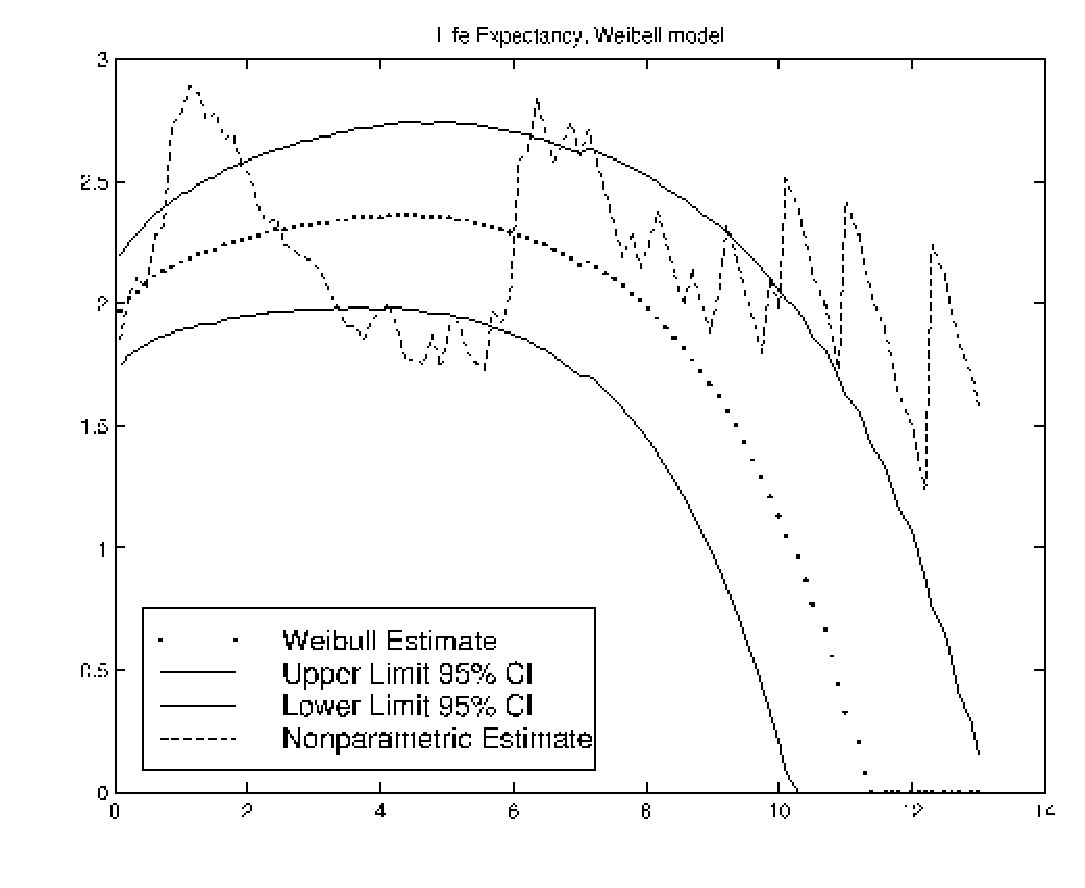
\includegraphics[width=6in]{Examples/Figures/weibull}
\end{figure}
In the figure one can see that the model doesn't fit the data well, in that it predicts life expectancy quite differently than does the nonparametric model. For ages 4-6, the nonparametric estimate is outside the confidence interval that results from the parametric model, which casts doubt upon the parametric model. Mongooses that are between 2-6 years old seem to have a lower life expectancy than is predicted by the Weibull model, whereas young mongooses that survive beyond infancy have a higher life expectancy, up to a bit beyond 2 years. Due to the dramatic change in the death rate as a function of $t$, one might specify $f_{D}(t)$ as a mixture of two Weibull densities, 
\[
f_{D}(t|\theta)=\delta\left(e^{-\left(\lambda_{1}t\right)^{\gamma_{1}}}\lambda_{1}\gamma_{1}(\lambda_{1}t)^{\gamma_{1}-1}\right)+\left(1-\delta\right)\left(e^{-\left(\lambda_{2}t\right)^{\gamma_{2}}}\lambda_{2}\gamma_{2}(\lambda_{2}t)^{\gamma_{2}-1}\right).
\]
 The parameters $\gamma_{i}$ and $\lambda_{i},i=1,2$ are the parameters of the two Weibull densities, and $\delta$ is the parameter that mixes the two.

With the same data, $\theta$ can be estimated using the mixed model. The results are a log-likelihood = -623.17. Note that a standard likelihood ratio test cannot be used to chose between the two models, since under the null that $\delta=1$ (single density), the two parameters $\lambda_{2}$ and $\gamma_{2}$ are not identified. It is possible to take this into account, but this topic is out of the scope of this course. Nevertheless, the improvement in the likelihood function is considerable. The parameter estimates are

\begin{center}
\begin{tabular}{lll}
 Parameter  &  Estimate  &  St. Error \tabularnewline
 $\lambda_{1}$ &  0.233  &  0.016 \tabularnewline
 $\gamma_{1}$ &  1.722  &  0.166 \tabularnewline
 $\lambda_{2}$ &  1.731  &  0.101 \tabularnewline
 $\gamma_{2}$ &  1.522  &  0.096 \tabularnewline
 $\delta$ &  0.428  &  0.035 \tabularnewline
\end{tabular}
\par\end{center}

\noindent Note that the mixture parameter is highly significant. This model leads to the fit in Figure \ref{mixed weibull}. Note that the parametric and nonparametric fits are quite close to one another, up to around $6$ years. The disagreement after this point is not too important, since less than 5\% of mongooses live more than 6 years, which implies that the Kaplan-Meier nonparametric estimate has a high variance (since it's an average of a small number of observations).
\begin{figure}
\caption{\label{mixed weibull}Life expectancy of mongooses, mixed Weibull model}


\includegraphics[width=6in]{Examples/Figures/mixed}
\end{figure}


Mixture models are often an effective way to model complex responses, though they can suffer from overparameterization. Alternatives will be discussed later.

For examples of MLE using the Poisson model applied to count data, see Section \ref{sub:MEPS data} in the chapter on Numerical Optimization. You should examine the scripts and run them to see how MLE is actually done, and how parameter standard errors are estimated. \newpage{}


\subsection{\label{sub:DSGE-ML}Estimation of a simple DSGE model}

Dynamic stochastic general equilibrium (DSGE) models are widely used tools in macroeconomics. These are models in which current decisions depend upon expectations of future events. An example is the simple real business cycle model discussed in \htmladdnormallink{Fern�ndez-Villaverde's RBC example}{http://www.dynare.org/documentation-and-support/examples/rbc.pdf}, which is available on the Dynare web page \url{www.dynare.org}. The file  \htmladdnormallink{EstimateRBC\_ML.mod}{file:///home/michael/Mystuff/Econometrics/Examples/RBC/EstimateRBC\_ML.mod}  shows how this model may be estimated, using maximum likelihood methods. The estimation process involves forming a linear approximation to the true model, which means that the estimator is not actually the true maximum likelihood estimator, it is actually a ''quasi-ML'' estimator. The quasi-likelihood is computed by putting the linearized model in state-space form, and then computing the likelihood iteratively using Kalman filtering, which relies on the assumption that shocks to the model are normally distributed. State space models and Kalman filtering are introduced in Section \ref{sec:State-space-models}. Once the likelihood function is available, the methods studied in this Chapter may be applied. 
\begin{itemize}
\item The linearization of the model, combined with the fact that it has only one shock, leads to a problem of ''stochastic singularity'', which means that only a single observed variable may be used to compute the likelihood function. If interested, do a Google search for this term, along with DSGE, and you'll find more information.
\item Not using all of the observed variables for estimation is very likely to cause problems of lack of identification and inefficiency. This can be confirmed if you experiment with the estimation script. This is not a problem of the ML method, it is a problem due to the fact that we are not really estimating the true model, we're working with a linear approximation. 
\item The intention of presenting this example is to show that ML may be used for estimation of complex models. The problem here is that the model is not complex enough: the linearization throws away so much information so that estimation becomes impossible. A better solution is to try to actually to ML estimation for the true nonlinear model: see papers by Fernandez-Villaverde and Rubio-Ramirez which use particle filtering for that. You can also modify the script to do this, as Dynare supports this option.\newpage{}
\end{itemize}

\section{Exercises}
\begin{enumerate}
\item Consider coin tossing with a single possibly biased coin. The density function for the random variable $y=1(heads)$ is 
\begin{eqnarray*}
f_{Y}(y,p_{0}) & = & p_{0}^{y}\left(1-p_{0}\right)^{1-y},y\in\{0,1\}\\
 & = & 0,y\notin\{0,1\}
\end{eqnarray*}
Suppose that we have a sample of size $n$. We know from above that the ML estimator is $\widehat{p_{0}}=\bar{y}$. We also know from the theory above that 
\[
\sqrt{n}\left(\bar{y}-p_{0}\right)\overset{a}{\sim}N\left[0,\mathcal{J}_{\infty}(p_{0})^{-1}\mathcal{I}_{\infty}(p_{0})\mathcal{J}_{\infty}(p_{0})^{-1}\right]
\]
\textbf{a)} find the analytic expression for $g_{t}(\theta)$ and show that $\mathcal{E}_{\theta}\left[g_{t}(\theta)\right]=0$\\
\textbf{b)} find the analytical expressions for $\mathcal{J}_{\infty}(p_{0})$ and $\mathcal{I}_{\infty}(p_{0})$ for this problem \\
\textbf{c)} verify that the result for $\lim Var\sqrt{n}\left(\hat{p}-p\right)$ found in section \ref{sub:Coin-flipping,-again} is equal to $\mathcal{J}_{\infty}(p_{0})^{-1}\mathcal{I}_{\infty}(p_{0})\mathcal{J}_{\infty}(p_{0})^{-1}$\\
\textbf{d)} Write an Octave program that does a Monte Carlo study that shows that $\sqrt{n}\left(\bar{y}-p_{0}\right)$ is approximately normally distributed when $n$ is large. Please give me histograms that show the sampling frequency of $\sqrt{n}\left(\bar{y}-p_{0}\right)$ for several values of $n$.
\item The exponential density is 
\[
f_{X}(x)=\left\{ \begin{array}{c}
\lambda e^{-\lambda x},\,x\geqslant0\\
0,\,x<0
\end{array}\right.
\]
Suppose we have an independently and identically distributed sample of size $n$, $\left\{ x_{i}\right\} ,i=1,2,...,n$, where each $x_{i}$ follows this exponential distribution. 

\begin{enumerate}
\item write the log likelihood function
\item compute the maximum likelihood estimator of the parameter $\lambda$.
\item explain how to estimate the asymptotic variance of the ML estimator. That is, if $\sqrt{n}\left(\hat{\lambda}-\lambda\right)\rightarrow^{d}N(0,V_{\infty})$, give a consistent estimator of $V_{\infty}$.
\end{enumerate}
\item Suppose we have an i.i.d. sample of size $n$ from the Poisson density. The Poisson density is $f_{y}(y;\lambda)=\frac{e^{-\lambda}\lambda^{y}}{y!}$. Verify that the ML estimator is asymptotically distributed as $\sqrt{n}\left(\hat{\lambda}-\lambda_{0}\right)\stackrel{d}{\rightarrow}N(0,\lambda_{0})$, where $\lambda_{0}$ is the true parameter value. Hint: compute the asymptotic variance using $-\mathcal{J}_{\infty}(\lambda_{0})^{-1}$. 
\item Consider the model $y_{t}=x_{t}^{\prime}\beta+\alpha\epsilon_{t}$ where the errors follow the Cauchy (Student-t with 1 degree of freedom) density. So 
\[
f(\epsilon_{t})=\frac{1}{\pi\left(1+\epsilon_{t}^{2}\right)},-\infty<\epsilon_{t}<\infty
\]
The Cauchy density has a shape similar to a normal density, but with much thicker tails. Thus, extremely small and large errors occur much more frequently with this density than would happen if the errors were normally distributed. Find the score function $g_{n}(\theta)$ where $\theta=\left(\begin{array}{cc}
\beta^{\prime} & \alpha\end{array}\right)^{\prime}$. 
\item Consider the model classical linear regression model $y_{t}=x_{t}^{\prime}\beta+\epsilon_{t}$ where $\epsilon_{t}\sim IIN(0,\sigma^{2})$. Find the score function $g_{n}(\theta)$ where $\theta=\left(\begin{array}{cc}
\beta^{\prime} & \sigma\end{array}\right)^{\prime}$.
\item Compare the first order conditions that define the ML estimators of problems 4 and 5 and interpret the differences. \emph{Why} are the first order conditions that define an efficient estimator different in the two cases?
\item Assume a d.g.p. follows the logit model: $\Pr(y=1|x)=\left(1+exp(-\beta^{0}x)\right)^{-1}$. 

\begin{enumerate}
\item Assume that $x\sim$ uniform(-a,a). Find the asymptotic distribution of the ML estimator of $\beta^{0}$ (this is a scalar parameter).
\item Now assume that $x\sim$ uniform(-2a,2a). Again find the asymptotic distribution of the ML estimator of $\beta^{0}$.
\item Comment on the results
\end{enumerate}
\item There is an ML estimation routine in the provided software that accompanies these notes. Edit (to see what it does) then run the script \href{https://github.com/mcreel/Econometrics/blob/master/MyOctaveFiles/Econometrics/MLE/mle_example.m}{mle\_{}example.m}. Interpret the output.
\item Estimate the simple Nerlove model discussed in section \ref{sub:The-Nerlove-data} by ML, assuming that the errors are i.i.d. $N(0,\sigma^{2})$ and compare to the results you get from running  \htmladdnormallink{Nerlove.m}{file:///home/michael/Mystuff/Econometrics/Examples/OLS/Nerlove.m} .
\item Using fmincon (Matlab) or sqp (Octave)

\begin{enumerate}
\item estimate the Nerlove model with the restriction that $\beta_{L}+\beta_{F}+\beta_{K}=1$ (the cost function satisfies homogeneity of degree one in factor prices). Test this restriction using the likelihood ratio test.
\item test the restriction that $\beta_{Q}=\text{1 (the model exhibits constant returns to scale) using the LR test}$.
\item test homogeneity of degree 1 and constant returns to scale jointly, using the LR test.
\end{enumerate}
\item Using \htmladdnormallink{logit.m}{file:///home/michael/Mystuff/Econometrics/MyOctaveFiles/Count/Logit.m}  and \htmladdnormallink{EstimateLogit.m}{file:///home/michael/Mystuff/Econometrics/Examples/NonlinearOptimization/EstimateLogit.m}  as templates, write a function to calculate the probit log likelihood, and a script to estimate a probit model. Run it using data that actually follows a logit model (you can generate it in the same way that is done in the logit example).
\item Study \texttt{mle\_results.m} to see what it does. Examine the functions that \texttt{mle\_results.m} calls, and in turn the functions that those functions call. Write a complete description of how the whole chain works.
\item In Subsection \ref{sub:MEPS data} a model is presented for data on health care usage, along with some Octave scripts. Look at the Poisson estimation results for the OBDV measure of health care use and give an economic interpretation. Estimate Poisson models for the other 5 measures of health care usage, using the provided scripts.
\item For practice using fminunc, estimate a Poisson model by ML using the 10 independent data points\\
 %
\begin{tabular}{|c|c|c|c|c|c|c|c|c|c|c|}
\hline 
y & 0 & 0 & 0 & 1 & 1 & 1 & 2 & 2 & 2 & 3\tabularnewline
\hline 
\hline 
x & -1 & -1 & 1 & 0 & -1 & -1 & 1 & 1 & 2 & 2\tabularnewline
\hline 
\end{tabular}. \\
For the Poisson model, the density $f_{Y}(y|x)=\frac{\exp(-\lambda)\lambda^{y}}{y!},$ $y=0,1,2,...$. To make the model depend on conditioning variables, use the parameterization $\lambda(x)=\exp(\theta_{1}+\theta_{2}x)$. The example EstimatePoisson.m, in the notes, should be helpful

\begin{enumerate}
\item create a data file that contains these observations
\item find the log-likelihood function
\item find the score function
\item write a Matlab function that computes the log-likelihood function, using the form obj=loglik(theta, data)
\item use fminunc to find the ML estimator. You need to use an anonymous function for this.
\item find the analytic expression for the ML estimator
\item compute the ML estimator using your analytic expression. It should be very close to what you got using fminunc. Is it? If not, revise your code to make it work better.
\end{enumerate}
\end{enumerate}
\newpage{}


\chapter{\label{cha:Generalized-method-of}Generalized method of moments}

\textbf{Readings}: Cameron and Trivedi, Ch. 6; Hamilton Ch. 14$^{*}$; Davidson and MacKinnon, Ch. 17 (see pg. 587 for refs. to applications), \cite{hansen1982},  \cite{NeweyMcfadden}\newpage{}


\section{Moment conditions}
\begin{defn}
Moment condition: a moment condition $m_{n}(\theta)=m_{n}(Z_{n},\theta)$ is a vector-valued function of the data $Z_{n}$ and the parameter $\theta$ that has mean zero, under the model, when evaluated at the true parameter value $\theta_{0}$, and expectation different from zero when evaluated at other parameter values: 
\begin{align*}
Em_{n}(Z_{n},\theta_{0}) & =0\\
Em_{n}(Z_{n},\theta) & \ne0,\,\theta\ne\theta_{0}
\end{align*}
\end{defn}
\begin{itemize}
\item The expectation operator $E$ means that expectations are taken with respect to the true density of the data. This may depend on more parameters than appear in $\theta$.
\item The statistic may be vector-valued, with dimension $G,$ say.\newpage{}\end{itemize}
\begin{defn}
Moment contribution: we will be dealing with moment conditions that are defined as averages: $m_{n}(\theta)=\frac{1}{n}\sum_{t}m(Z_{t},\theta)=\frac{1}{n}\sum_{t}m_{t}(\theta)$. The functions $m_{t}(\theta)$ are the \emph{moment contributions.} The $t$th moment contribution $m_{t}$ is a function the same observation's data. I'm casually using $m(Z_{t},\theta),$ $m_{t}(\theta)$ and $m_{t}$ to all refer to the same thing. This first of these is the full expression, but I will suppress arguments when the context makes things clear enough, to reduce the notational burden. The main thing is that $m_{n}$ refers to the average over the $n$ observations, and $m_{t}$ refers to the terms that are averaged. \newpage{}\end{defn}
\begin{example}
OLS. The classical linear model. Let $m_{n}(\beta)=\frac{1}{n}\sum_{t}x_{t}(y_{t}-x_{t}^{\prime}\beta).$ So the moment contributions are $m_{t}(\beta)=x_{t}(y_{t}-x_{t}^{\prime}\beta)$. When $\beta=\beta_{0},$ $y_{t}-x_{t}^{\prime}\beta_{0}=\epsilon_{t},$ and $m_{t}=x_{t}\epsilon_{t}$. We know that $E(x_{t}\epsilon_{t})=0,$ by the weak exogeneity assumption. Thus, the moment contributions, and the moment condition, which is their average, have expectation zero when evaluated at the true parameter value.\newpage{}
\end{example}
$\,$
\begin{example}
ML. We have seen (see eqn. \ref{eq:ExpectationScore}) that the score contributions of the ML estimator have mean zero: $E\left(D_{\theta}\ln f(y_{t}|x_{x},\theta_{0})\right)=0$. So, we could set $m_{t}(\theta)=D_{\theta}\ln f(y_{t}|x_{x},\theta)$.\newpage{}
\end{example}
$\,$
\begin{example}
Sampling from $\chi^{2}.$ Suppose we draw a random sample of $y_{t}$ from the $\chi^{2}(\theta_{0})$ distribution. Here, $\theta_{0}$ is the parameter of interest. If $Y\sim\chi^{2}(\theta_{0})$, then the mean $E(Y)=\theta_{0}$. Let the moment contribution be 

\[
m_{t}(\theta)=y_{t}-\theta
\]
Then 
\begin{align*}
m_{n}(\theta) & =\frac{1}{n}\sum_{t=1}^{n}m_{t}(\theta)=\bar{y}-\theta
\end{align*}
We know that the $E(\bar{y})=\theta_{0}.$ Thus, $Em_{n}(\theta_{0})=0.$ However, $Em_{n}(\theta)=\theta_{0}-\theta\ne$0 if $\theta\ne\theta_{0}.$ \newpage{}
\end{example}
When the dimension of the moment conditions is the same as the dimension of the parameter vector $\theta$, the \emph{method of moments principle} is to choose the estimator of the parameter to \emph{set the moment condition equal to zero}: $m_{n}(\hat{\theta})\equiv0$. Then the equation is solved for the estimator. In the case of OLS, this gives $\sum_{t}x_{t}(y_{t}-x_{t}^{\prime}\hat{\beta})=0,$ which gives a solution that you should already know. For the chi-squared example, 
\[
m(\hat{\theta})=\bar{y}-\hat{\theta}=0
\]
is solved by $\hat{\theta}=\bar{y}$. Since $\bar{y}=\sum_{t=1}^{n}y_{t}/n\stackrel{p}{\rightarrow}\theta^{0}$ by the LLN, the estimator is consistent.\newpage{}
\begin{example}
$\chi^{2},$ version 2. The variance of a $\chi^{2}(\theta^{0})$ r.v. is 
\[
V\left(Y\right)=E_{\theta^{0}}\left(Y-\theta^{0}\right)^{2}=2\theta^{0}.
\]


Let 
\begin{align*}
m_{t}(\theta) & =\left(y_{t}-\bar{y}\right)^{2}-2\theta
\end{align*}


The MM estimator using the variance would set 
\[
m_{n}(\hat{\theta})=\frac{\sum_{t=1}^{n}\left(y_{t}-\bar{y}\right)^{2}}{n}-2\hat{\theta}\equiv0.
\]
Solving for the estimator, it is half the sample variance (dividing by $n$ rather than the bias correcting $n-1)$: 
\[
\hat{\theta}=\frac{1}{2}\frac{\sum_{t=1}^{n}\left(y_{t}-\bar{y}\right)^{2}}{n}.
\]
Again, by the LLN, the sample variance is consistent for the true variance, that is, 
\[
\frac{\sum_{t=1}^{n}\left(y_{t}-\bar{y}\right)^{2}}{n}\stackrel{p}{\rightarrow}2\theta^{0}.
\]
So, this MM is also consistent for $\theta^{0}$. \newpage{}
\end{example}
$\,$
\begin{example}
\label{exa:chi2 mm}Try some MM estimation yourself: here's an Octave script that implements the two MM estimators discussed above:  \htmladdnormallink{GMM/chi2mm.m}{file:///home/michael/Mystuff/Econometrics/Examples/GMM/chi2mm.m}
\end{example}
Note that when you run the script, the two estimators give different results. Each of the two estimators is consistent. 
\begin{itemize}
\item For the $\chi^{2}$ example, we have two alternative moment conditions and only one parameter: we have \emph{overidentification,} which means that we have more information than is strictly necessary for consistent estimation of the parameter.
\item The idea behind GMM is to combine information from the two moment conditions to form a new estimator which will be\emph{\ more efficient,} in general (proof of this below).
\item Note that the fact that the data has a chi-squared distribution is not used in estimation, it just as easily could have been normally distributed, sampling from a $N(\theta_{0},2\theta_{0})$ distribution. As long as the assumptions regarding the mean or variance are correct, the MM estimators are consistent. So, we don't make use of distributional assumptions when doing method of moment estimation, we only rely on certain moments being correctly specified. In this way, method of moments estimation is \emph{more robust} than is maximum likelihood estimation: we obtain a consistent estimator with fewer assumptions. There being no free lunch, we should expect to pay something for this, of course. The cost will be a loss of efficiency, in general.\newpage{}
\end{itemize}
\textbf{To summarize}, a moment condition is a vector valued function which has expectation zero at the true parameter value. We have seen some examples of where we might get such functions, and more will follow. For now, let's take moment conditions as given, and work out the properties of the estimator.\newpage{}


\section{Definition of GMM estimator}

For the purposes of this course, the following definition of the GMM estimator is sufficiently general:
\begin{defn}
\label{GMM estimator (defn)}The GMM estimator of the $k$ -dimensional parameter vector $\theta_{0},$ $\hat{\theta}\equiv\arg\min_{\Theta}s_{n}(\theta)\equiv m_{n}(\theta)^{\prime}W_{n}m_{n}(\theta),$ where $m_{n}(\theta)=\frac{1}{n}\sum_{t=1}^{n}m(Z_{t},\theta)$ is a $g$-vector valued function of the , $g\geq k,$ with $\mathcal{E}m(\theta_{0})=0,$ and $W_{n}$ converges almost surely to a finite $g\times g$ symmetric positive definite matrix $W_{\infty}$. \newpage{}
\end{defn}
\emph{What's the reason for using GMM if MLE is asymptotically efficient?} 
\begin{itemize}
\item Robustness: GMM is based upon a limited set of moment conditions. For consistency, only these moment conditions need to be correctly specified, whereas MLE in effect requires correct specification of \emph{every conceivable} moment condition. GMM is \emph{robust with respect to distributional misspecification.} The price for robustness is usually a loss of efficiency with respect to the MLE estimator. Keep in mind that the true distribution is \uline{not known} so if we erroneously specify a distribution and estimate by MLE, the estimator will be inconsistent in general (not always). 
\item Feasibility: in some cases the MLE estimator is not available, because we are not able to deduce or compute the likelihood function. More on this in the section on simulation-based estimation. The GMM estimator may still be feasible even though MLE is not available.\newpage{}\end{itemize}
\begin{example}
The Octave script  \htmladdnormallink{GMM/chi2gmm.m}{file:///home/michael/Mystuff/Econometrics/Examples/GMM/chi2gmm.m} implements GMM using the same $\chi^{2}$ data as was using in Example \ref{exa:chi2 mm}, above. The two moment conditions, based on the sample mean and sample variance are combined. The weight matrix is an identity matrix, $I_{2}.$ In Octave, type ''help gmm\_estimate'' to get more information on how the GMM estimation routine works.\newpage{}
\end{example}

\section{Consistency}

We simply assume that the assumptions of Theorem \ref{Consistency of ee} hold, so the GMM estimator is strongly consistent. The main requirement is that the moment conditions have mean zero at the true parameter value, $\theta^{0}.$ This will be the case if our moment conditions are correctly specified. With this, it is clear that the minimum of the limiting objective function occurs at the true parameter value. The only assumption that warrants additional comment is that of identification. In Theorem \ref{Consistency of ee}, the third assumption reads: (c) \textit{Identification:} $s_{\infty}(\cdot)$ has a unique global maximum at $\theta^{0},$ \textit{i.e.,} $s_{\infty}(\theta^{0})>s_{\infty}(\theta),$ $\forall\theta\neq\theta^{0}.$ Taking the case of a quadratic objective function $s_{n}(\theta)=m_{n}(\theta)^{\prime}W_{n}m_{n}(\theta),$ first consider $m_{n}(\theta).$
\begin{itemize}
\item Applying a uniform law of large numbers, we get $m_{n}(\theta)\stackrel{a.s.}{\rightarrow}m_{\infty}(\theta).$
\item Since $\mathcal{E}_{\theta^{0}}m_{n}(\theta^{0})=0$ by assumption, $m_{\infty}(\theta^{0})=0.$
\item Since $s_{\infty}(\theta^{0})=m_{\infty}(\theta^{0})^{\prime}W_{\infty}m_{\infty}(\theta^{0})=0,$ in order for asymptotic identification, we need that $m_{\infty}(\theta)\neq0$ for $\theta\neq\theta^{0},$ for at least some element of the vector. There can be no other parameter value that sets the moment conditions to zero (at least, in the limit). This and the assumption that $W_{n}\stackrel{a.s.}{\rightarrow}$ $W_{\infty},$ a finite positive $g\times g$ definite $g\times g$ matrix guarantee that $\theta^{0}$ is asymptotically identified.
\item Note that asymptotic identification does not rule out the possibility of lack of identification for a given data set - there may be multiple minimizing solutions in finite samples. \newpage{}\end{itemize}
\begin{example}
Increase $n$ in the Octave script  \htmladdnormallink{GMM/chi2gmm.m}{file:///home/michael/Mystuff/Econometrics/Examples/GMM/chi2gmm.m} to see evidence of the consistency of the GMM estimator.\newpage{}
\end{example}

\section{Asymptotic normality}

We also simply assume that the conditions of Theorem \ref{Normality of ee} hold, so we will have asymptotic normality. However, we do need to find the structure of the asymptotic variance-covariance matrix of the estimator. From Theorem \ref{Normality of ee}, we have 
\[
\sqrt{n}\left(\hat{\theta}-\theta^{0}\right)\stackrel{d}{\rightarrow}N\left[0,\mathcal{J}_{\infty}(\theta^{0})^{-1}\mathcal{I}_{\infty}(\theta^{0})\mathcal{J}_{\infty}(\theta^{0})^{-1}\right]
\]
 where $\mathcal{J}_{\infty}(\theta^{0})$ is the almost sure limit of $\frac{\partial^{2}}{\partial\theta\partial\theta^{\prime}}s_{n}(\theta)$ when evaluated at $\theta^{0}$ and 
\[
\mathcal{I}_{\infty}(\theta^{0})=\lim_{n\rightarrow\infty}Var\sqrt{n}\frac{\partial}{\partial\theta}s_{n}(\theta^{0}).
\]
 We need to determine the form of these matrices given the objective function $s_{n}(\theta)=m_{n}(\theta)^{\prime}W_{n}m_{n}(\theta).$

Now, using the product rule from section \ref{sec:Notation-for-differentiation}, 
\[
\frac{\partial}{\partial\theta}s_{n}(\theta)=2\left[\frac{\partial}{\partial\theta}m_{n}^{^{\prime}}\left(\theta\right)\right]W_{n}m_{n}\left(\theta\right)
\]
 (this is analogous to $\frac{\partial}{\partial\beta}\beta^{\prime}X^{\prime}X\beta=2X^{\prime}X\beta$ which appears when computing the first order conditions for the OLS estimator).

Define the $k\times g$ matrix 
\[
D_{n}(\theta)\equiv\frac{\partial}{\partial\theta}m_{n}^{\prime}\left(\theta\right),
\]
 so:
\begin{equation}
\frac{\partial}{\partial\theta}s(\theta)=2D(\theta)Wm\left(\theta\right).\label{gmmscores}
\end{equation}
 (Note that $s_{n}(\theta)$, $D_{n}(\theta),$ $W_{n}$ and $m_{n}(\theta)$ all depend on the sample size $n,$ but it is omitted to unclutter the notation).

To take second derivatives, let $D_{i}$ be the $i-$ th row of $D(\theta).$ This is a $1\times G$ row vector, and 
\[
\frac{\partial}{\partial\theta_{i}}s(\theta)=2D_{i}(\theta)Wm\left(\theta\right)
\]
\textbf{is a scalar}, which is the $i$th row of the column vector $\frac{\partial}{\partial\theta}s(\theta)$. The $i$th row of the matrix of second derivatives is (using the product rule in definition \ref{def: Product-rule.-Let}), 
\begin{eqnarray*}
\frac{\partial}{\partial\theta^{\prime}}\frac{\partial}{\partial\theta_{i}}s(\theta) & = & \frac{\partial}{\partial\theta^{\prime}}\left[2D_{i}(\theta)Wm\left(\theta\right)\right]\\
 & = & 2D_{i}WD^{\prime}+2m^{\prime}W\left[\frac{\partial}{\partial\theta^{\prime}}D_{i}^{\prime}\right]
\end{eqnarray*}
Note that the first term contains a $D^{\prime},$ which appears due to $\frac{\partial}{\partial\theta^{\prime}}m_{n}\left(\theta\right)$. When evaluating the second term: 
\[
2m(\theta)^{\prime}W\left[\frac{\partial}{\partial\theta^{\prime}}D(\theta)_{i}^{\prime}\right]
\]
(where the dependence of $D$ upon $\theta$ is emphasized) at $\theta^{0},$ assume that $\frac{\partial}{\partial\theta^{\prime}}D(\theta)_{i}^{\prime}$ satisfies a LLN (it is an average), so that it converges almost surely to a finite limit. In this case, we have 
\[
2m(\theta^{0})^{\prime}W\left[\frac{\partial}{\partial\theta^{\prime}}D(\theta^{0})_{i}^{\prime}\right]\stackrel{a.s.}{\rightarrow}0,
\]
because $m(\theta^{0})=o_{p}(1)$ and $W\stackrel{a.s.}{\rightarrow}$ $W_{\infty}$.

Stacking these results over the $k$ rows of $D,$ we get 
\[
\lim\frac{\partial^{2}}{\partial\theta\partial\theta^{\prime}}s_{n}(\theta^{0})=\mathcal{J}_{\infty}(\theta^{0})=2D_{\infty}W_{\infty}D_{\infty}^{\prime},a.s.,
\]
 where we define $\lim D=D_{\infty},$ $a.s.,$ and $\lim W=W_{\infty},$ a.s. (we assume a LLN holds).

With regard to $\mathcal{I}_{\infty}(\theta^{0})$, following equation \ref{gmmscores}, and noting that the scores have mean zero at $\theta^{0}$ (since $\mathcal{E}m(\theta^{0})=0$ by assumption), we have
\begin{eqnarray*}
\mathcal{I}_{\infty}(\theta^{0}) & = & \lim_{n\rightarrow\infty}Var\sqrt{n}\frac{\partial}{\partial\theta}s_{n}(\theta^{0})\\
 & = & \lim_{n\rightarrow\infty}\mathcal{E}4nDWm(\theta^{0})m(\theta^{0})^{\prime}WD^{\prime}\\
 & = & \lim_{n\rightarrow\infty}\mathcal{E}4DW\left\{ \sqrt{n}m(\theta^{0})\right\} \left\{ \sqrt{n}m(\theta^{0})^{\prime}\right\} WD^{\prime}
\end{eqnarray*}
 Now, given that $m(\theta^{0})$ is an average of centered (mean-zero) quantities, it is reasonable to expect a CLT to apply, after multiplication by $\sqrt{n}$. Assuming this, 
\begin{equation}
\sqrt{n}m(\theta^{0})\stackrel{d}{\rightarrow}N(0,\Omega_{\infty}),\label{eq:CLT applied to moment conditions}
\end{equation}
 where 
\[
\Omega_{\infty}=\lim_{n\rightarrow\infty}\mathcal{E}\left[nm(\theta^{0})m(\theta^{0})^{\prime}\right].
\]
 Using this, and the last equation, we get 
\[
\mathcal{I}_{\infty}(\theta^{0})=4D_{\infty}W_{\infty}\Omega_{\infty}W_{\infty}D_{\infty}^{\prime}
\]
 Using these results, the asymptotic normality theorem (\ref{Normality of ee}) gives us 
\[
\sqrt{n}\left(\hat{\theta}-\theta^{0}\right)\stackrel{d}{\rightarrow}N\left[0,\left(D_{\infty}W_{\infty}D_{\infty}^{\prime}\right)^{-1}D_{\infty}W_{\infty}\Omega_{\infty}W_{\infty}D_{\infty}^{\prime}\left(D_{\infty}W_{\infty}D_{\infty}^{\prime}\right)^{-1}\right],
\]
 the asymptotic distribution of the GMM estimator for arbitrary weighting matrix $W_{n}.$ Note that for $J_{\infty}$ to be positive definite, $D_{\infty}$ must have full row rank, $\rho(D_{\infty})=k$. This is related to identification. If the rows of $m_{n}(\theta)$ were not linearly independent of one another, then neither $D_{n}$ nor $D_{\infty}$ would have full row rank. Identification plus two times differentiability of the objective function lead to $J_{\infty}$ being positive definite.

There are two things that affect the asymptotic variance:
\begin{itemize}
\item the choice of the moment conditions, $m_{n}(\theta$), which determines both $D_{\infty}$ and $\Omega_{\infty}$
\item the choice of the weight matrix $W_{n}$, which determines $W_{\infty}$
\end{itemize}
We would probably like to know how to choose both $m_{n}(\theta)$ and $W_{n}$ so that the asymptotic variance is a small as possible.\newpage{}
\begin{example}
The Octave script  \htmladdnormallink{GMM/AsymptoticNormalityGMM.m}{file:///home/michael/Mystuff/Econometrics/Examples/GMM/AsymptoticNormalityGMM.m} does a Monte Carlo of the GMM estimator for the $\chi^{2}$ data. Histograms for 1000 replications of $\sqrt{n}\left(\hat{\theta}-\theta^{0}\right)$ are given in Figure \ref{fig:Asymptotic-Normality-of}. On the left are results for $n=10,$ on the right are results for $n=1000.$ Note that the two distributions are more or less centered at 0. The distribution for the small sample size is somewhat asymmetric, which shows that the small sample distribution may be poorly approximated by the asymptotic distribution. This has mostly disappeared for the larger sample size.\newpage{} 
\begin{figure}
\caption{\label{fig:Asymptotic-Normality-of}Asymptotic Normality of GMM estimator, $\chi^{2}$ example}


\subfloat[$n=10$]{

\includegraphics[width=10cm]{Examples/GMM/AsNorm_n10}

}\subfloat[$n=1000$]{

\includegraphics[width=10cm]{Examples/GMM/AsNorm_n1000}

}

\end{figure}
\newpage{}
\end{example}

\section{Choosing the weighting matrix}

$W$ is a \textit{weighting matrix,} which determines the relative importance of violations of the individual moment conditions. For example, if we are much more sure of the first moment condition, which is based upon the variance, than of the second, which is based upon the fourth moment, we could set 
\[
W=\left[\begin{array}{cc}
a & 0\\
0 & b
\end{array}\right]
\]
 with $a$ much larger than $b.$ In this case, errors in the second moment condition have less weight in the objective function.
\begin{itemize}
\item Since moments are not independent, in general, we should expect that there be a correlation between the moment conditions, so it may not be desirable to set the off-diagonal elements to 0. $W$ may be a random, data dependent matrix.
\item We have already seen that the choice of $W$ will influence the asymptotic distribution of the GMM estimator. Since the GMM estimator is already inefficient w.r.t. MLE, we might like to choose the $W$ matrix to make the GMM\ estimator efficient \emph{within the class of GMM estimators} defined by $m_{n}(\theta)$.
\item To provide a little intuition, consider the linear model $y=\mathbf{x}^{\prime}\beta+\varepsilon,$ where $\varepsilon\sim N(0,\Omega).$ That is, he have heteroscedasticity and autocorrelation.
\item Let $P$ be the Cholesky factorization of $\Omega^{-1},$ e.g, $P^{\prime}P=\Omega^{-1}.$
\item Then the model $Py=P\mathbf{X}\beta+P\varepsilon$ satisfies the classical assumptions of homoscedasticity and nonautocorrelation, because $V(P\varepsilon)=PV(\varepsilon)P^{\prime}=P\Omega P^{\prime}=P(P^{\prime}P)^{-1}P^{\prime}=PP^{-1}\left(P^{\prime}\right)^{-1}P^{\prime}=I_{n}.$ (Note: we use $\left(AB\right)^{-1}=B^{-1}A^{-1}$ for $A,$ $B$ both nonsingular). This means that the transformed model is efficient.
\item The OLS\ estimator of the model $Py=P\mathbf{X}\beta+P\varepsilon$ minimizes the objective function $(y-\mathbf{X}\beta)^{\prime}\Omega^{-1}(y-\mathbf{X}\beta).$ Interpreting $\left(y-\mathbf{X}\beta\right)=\varepsilon(\beta)$ as moment conditions (note that they do have zero expectation when evaluated at $\beta^{0}$), the optimal weighting matrix is seen to be the inverse of the covariance matrix of the moment conditions. This result carries over to GMM\ estimation. (Note:\ this presentation of GLS\ is not a GMM\ estimator as defined above, because the number of moment conditions here is equal to the sample size, $n.$ Later we'll see that GLS\ can be put into the GMM framework defined above). \end{itemize}
\begin{thm}
\label{efficient weighting matrix}If $\hat{\theta}$ is a GMM\ estimator that minimizes $m_{n}(\theta)^{\prime}W_{n}m_{n}(\theta),$ the asymptotic variance of $\hat{\theta}$ will be minimized by choosing $W_{n}$ so that $W_{n}\stackrel{a.s}{\rightarrow}W_{\infty}=\Omega_{\infty}^{-1},$ where $\Omega_{\infty}=\lim_{n\rightarrow\infty}\mathcal{E}\left[nm(\theta^{0})m(\theta^{0})^{\prime}\right].$

\textbf{Proof:} For $W_{\infty}=\Omega_{\infty}^{-1},$ the asymptotic variance 
\[
\left(D_{\infty}W_{\infty}D_{\infty}^{\prime}\right)^{-1}D_{\infty}W_{\infty}\Omega_{\infty}W_{\infty}D_{\infty}^{\prime}\left(D_{\infty}W_{\infty}D_{\infty}^{\prime}\right)^{-1}
\]
 simplifies to $\left(D_{\infty}\Omega_{\infty}^{-1}D_{\infty}^{\prime}\right)^{-1}.$ Now, let $A$ be the difference between the general form and the simplified form: 
\begin{eqnarray*}
A=\left(D_{\infty}W_{\infty}D_{\infty}^{\prime}\right)^{-1}D_{\infty}W_{\infty}\Omega_{\infty}W_{\infty}D_{\infty}^{\prime}\left(D_{\infty}W_{\infty}D_{\infty}^{\prime}\right)^{-1} & - & \left(D_{\infty}\Omega_{\infty}^{-1}D_{\infty}^{\prime}\right)^{-1}
\end{eqnarray*}
Set $B=\left(D_{\infty}W_{\infty}D_{\infty}^{\prime}\right)^{-1}D_{\infty}W_{\infty}-\left(D_{\infty}\Omega_{\infty}^{-1}D_{\infty}^{\prime}\right)^{-1}D_{\infty}\Omega_{\infty}^{-1}$. One can show that $A=B\Omega_{\infty}B^{'}$. This is a quadratic form in a p.d. matrix, so it is p.s.d., which concludes the proof. 

\end{thm}
The result

\begin{equation}
\sqrt{n}\left(\hat{\theta}-\theta^{0}\right)\stackrel{d}{\rightarrow}N\left[0,\left(D_{\infty}\Omega_{\infty}^{-1}D_{\infty}^{\prime}\right)^{-1}\right]\label{gmm distribution with optimal weighting matrix}
\end{equation}
 allows us to treat 
\[
\hat{\theta}\approx N\left(\theta^{0},\frac{\left(D_{\infty}\Omega_{\infty}^{-1}D_{\infty}^{\prime}\right)^{-1}}{n}\right),
\]
 where the $\approx$ means ''approximately distributed as.'' To operationalize this we need estimators of $D_{\infty}$ and $\Omega_{\infty}.$
\begin{itemize}
\item The obvious estimator of $\widehat{D_{\infty}}$ is simply $\frac{\partial}{\partial\theta}m_{n}^{\prime}\left(\hat{\theta}\right),$ which is consistent by the consistency of $\hat{\theta},$ assuming that $\frac{\partial}{\partial\theta}m_{n}^{\prime}$ is continuous in $\theta.$ Stochastic equicontinuity results can give us this result even if $\frac{\partial}{\partial\theta}m_{n}^{\prime}$ is not continuous.\end{itemize}
\begin{example}
To see the effect of using an efficient weight matrix, consider the Octave script  \htmladdnormallink{GMM/EfficientGMM.m}{file:///home/michael/Mystuff/Econometrics/Examples/GMM/EfficientGMM.m}. This modifies the previous Monte Carlo for the $\chi^{2}$ data. This new Monte Carlo computes the GMM estimator in two ways:\\
1) based on an identity weight matrix\\
2) using an estimated optimal weight matrix. The estimated efficient weight matrix is computed as the inverse of the estimated covariance of the moment conditions, using the inefficient estimator of the first step. See the next section for more on how to do this.\\
Figure \ref{fig:Inefficient-and-Efficient} shows the results, plotting histograms for 1000 replications of $\sqrt{n}\left(\hat{\theta}-\theta^{0}\right)$. Note that the use of the estimated efficient weight matrix leads to much better results in this case. This is a simple case where it is possible to get a good estimate of the efficient weight matrix. This is not always so. See the next section.

\begin{figure}


\caption{\label{fig:Inefficient-and-Efficient}Inefficient and Efficient GMM estimators, $\chi^{2}$ data}


\subfloat[inefficient]{



\includegraphics[width=10cm]{Examples/GMM/Inefficient}

}\subfloat[efficient]{

\includegraphics[width=10cm]{Examples/GMM/Efficient}}

\end{figure}



\end{example}

\section{Estimation of the variance-covariance matrix}

\textbf{(See Hamilton Ch. 10, pp. 261-2 and 280-84)}$^{*}$\textbf{.}

In the case that we wish to use the optimal weighting matrix, we need an estimate of $\Omega_{\infty},$ the limiting variance-covariance matrix of $\sqrt{n}m_{n}(\theta^{0})$. While one could think of estimating $\Omega_{\infty}$ parametrically (along the lines of feasible GLS) we in general have little information upon which to base a parametric specification, so nonparametric estimation is normally used. In general, we expect that:
\begin{itemize}
\item $m_{t}$ will be autocorrelated ($\Gamma_{ts}=\mathcal{E}(m_{t}m_{t-s}^{\prime})\neq0$). Note that this autocovariance will not depend on $t$ if the moment conditions are covariance stationary.
\item contemporaneously correlated, since the individual moment conditions will not in general be independent of one another ($\mathcal{E}(m_{it}m_{jt})\neq0$).
\item and have different variances ($\mathcal{E}(m_{it}^{2})=\sigma_{it}^{2}$ ). 
\end{itemize}
Since we need to estimate so many components if we are to take the parametric approach, it is unlikely that we would arrive at a correct parametric specification. For this reason, research has focused on consistent nonparametric estimators of $\Omega_{\infty}.$ 

Henceforth we assume that $m_{t}$ is \emph{covariance stationary} (the covariance between $m_{t}$ and $m_{t-s}$ does not depend on $t).$ Define the $s-th$ autocovariance of the moment conditions $\Gamma_{s}=\mathcal{E}(m_{t}m_{t-s}^{\prime}).$ 
\begin{xca}
Show that $\mathcal{E}(m_{t}m_{t+s}^{\prime})=\Gamma_{s}^{\prime}.$ 
\end{xca}
Recall that $m_{t}$ and $m_{n}$ are functions of $\theta,$ so for now assume that we have some consistent estimator of $\theta^{0}$. With this, a consistent estimator of $m_{t}(\theta^{0})$ is $\hat{m}_{t}=m_{t}(\hat{\theta}).$ Now 
\begin{eqnarray*}
\Omega_{n} & = & \mathcal{E}\left[nm_{n}(\theta^{0})m_{n}(\theta^{0})^{\prime}\right]=\mathcal{E}\left[n\left(1/n\sum_{t=1}^{n}m_{t}\right)\left(1/n\sum_{t=1}^{n}m_{t}^{\prime}\right)\right]\\
 & = & \mathcal{E}\left[1/n\left(\sum_{t=1}^{n}m_{t}\right)\left(\sum_{t=1}^{n}m_{t}^{\prime}\right)\right]\\
 & = & \Gamma_{0}+\frac{n-1}{n}\left(\Gamma_{1}+\Gamma_{1}^{\prime}\right)+\frac{n-2}{n}\left(\Gamma_{2}+\Gamma_{2}^{\prime}\right)\cdots+\frac{1}{n}\left(\Gamma_{n-1}+\Gamma_{n-1}^{\prime}\right)
\end{eqnarray*}
 A natural, consistent estimator of $\Gamma_{s}$ is 
\[
\widehat{\Gamma_{s}}=1/n\sum_{t=v+1}^{n}\hat{m}_{t}\hat{m}_{t-s}^{\prime}.
\]
 (you might use $n-s$ in the denominator instead). So, a natural, but inconsistent, estimator of $\Omega_{\infty}$ would be 
\begin{eqnarray*}
\hat{\Omega} & = & \widehat{\Gamma_{0}}+\frac{n-1}{n}\left(\widehat{\Gamma_{1}}+\widehat{\Gamma_{1}^{\prime}}\right)+\frac{n-2}{n}\left(\widehat{\Gamma_{2}}+\widehat{\Gamma_{2}^{\prime}}\right)+\cdots+\left(\widehat{\Gamma_{n-1}}+\widehat{\Gamma_{n-1}^{\prime}}\right)\\
 & = & \widehat{\Gamma_{0}}+\sum_{s=1}^{n-1}\frac{n-s}{n}\left(\widehat{\Gamma_{s}}+\widehat{\Gamma_{s}^{\prime}}\right).
\end{eqnarray*}
 This estimator is inconsistent in general, since the number of parameters to estimate is more than the number of observations, and increases more rapidly than $n$, so information does not build up as $n\rightarrow\infty.$

On the other hand, supposing that $\Gamma_{v}$ tends to zero sufficiently rapidly as $s$ tends to $\infty,$ a modified estimator is 
\[
\hat{\Omega}=\widehat{\Gamma_{0}}+\sum_{s=1}^{q(n)}\left(\widehat{\Gamma_{s}}+\widehat{\Gamma_{s}^{\prime}}\right).
\]

\begin{itemize}
\item this will be consistent, provided that

\begin{itemize}
\item $q(n)\stackrel{p}{\rightarrow}\infty$ as $n\rightarrow\infty$,
\item $q(n)$ grows sufficiently slowly.
\item The term $\frac{n-s}{n}$ can be dropped because it converges to 1.
\item A disadvantage of this estimator is that it may not be positive definite. This could cause one to calculate a negative $\chi^{2}$ statistic, for example!
\end{itemize}
\item Note: the formula for $\hat{\Omega}$ requires an estimate of $m(\theta^{0}),$ which in turn requires an estimate of $\theta,$ which is based upon an estimate of $\Omega!$ The solution to this circularity is to set the weighting matrix $W$ arbitrarily (for example to an identity matrix), obtain a first consistent but inefficient estimate of $\theta^{0},$ then use this estimate to form $\hat{\Omega},$ then re-estimate $\theta^{0}.$ The process can be iterated until neither $\hat{\Omega}$ nor $\hat{\theta}$ change appreciably between iterations. 
\end{itemize}

\subsection{Newey-West covariance estimator}

The Newey-West estimator (\cite{NeweyWest1987}) solves the problem of possible nonpositive definiteness of the above estimator. Their estimator is 
\[
\hat{\Omega}=\widehat{\Gamma_{0}}+\sum_{s=1}^{q(n)}\left[1-\frac{s}{q+1}\right]\left(\widehat{\Gamma_{s}}+\widehat{\Gamma_{s}^{\prime}}\right).
\]
 This estimator is p.d. by construction. The condition for consistency is that $n^{-1/4}q\rightarrow0.$ Note that this is a very slow rate of growth for $q.$ This estimator is nonparametric - we've placed no parametric restrictions on the form of $\Omega.$ It is an example of a \textit{kernel} estimator. Kernel estimators are discussed in more detail in Chapter \ref{chap:Nonparametric-inference}. Around the same time as the paper by Newey and West, a number of other similar covariance matrix estimators were proposed, but the NW estimator seems to be the most widely used in empirical work.


\section{Estimation using conditional moments}

So far, the moment conditions have been presented as unconditional expectations. One common way of defining unconditional moment conditions is based upon conditional moment conditions.

Suppose that a random variable $Y$ has zero expectation conditional on the random variable $X$
\[
\mathcal{E}_{Y|X}Y=\int Yf(Y|X)dY=0
\]
 Then the unconditional expectation of the product of $Y$ and a function $g(X)$ of $X$ is also zero. The unconditional expectation is 
\[
\mathcal{E}Yg(X)=\int_{\mathcal{X}}\left(\int_{\mathcal{Y}}Yg(X)f(Y,X)dY\right)dX.
\]
 This can be factored into a conditional expectation and an expectation w.r.t. the marginal density of $X:$
\[
\mathcal{E}Yg(X)=\int_{\mathcal{X}}\left(\int_{\mathcal{Y}}Yg(X)f(Y|X)dY\right)f(X)dX.
\]
 Since $g(X)$ doesn't depend on $Y$ it can be pulled out of the integral 
\[
\mathcal{E}Yg(X)=\int_{\mathcal{X}}\left(\int_{\mathcal{Y}}Yf(Y|X)dY\right)g(X)f(X)dX.
\]
 But the term in parentheses on the rhs is zero by assumption, so 
\[
\mathcal{E}Yg(X)=0
\]
 as claimed.

This is important from the point of view of constructing an econometric model, since economic models often imply restrictions on conditional moments.
\begin{itemize}
\item Suppose a model tells us that the function $K(y_{t},x_{t},\theta)$ has expectation, conditional on the information set $I_{t},$ equal to $k(x_{t},\theta),$
\[
\mathcal{E}_{\theta}K(y_{t},x_{t},\theta)|I_{t}=k(x_{t},\theta).
\]


\begin{itemize}
\item For example, in the context of the classical linear model $y_{t}=x_{t}^{\prime}\beta+\varepsilon_{t},$ we can set $K(y_{t},x_{t},\theta)=y_{t}$ so that $k(x_{t},\theta)=x_{t}^{\prime}\beta$.
\item In the case of the simultaneous equations model of equation \ref{eq:demand function}, we have
\[
q_{t}=\alpha_{1}+\alpha_{2}p_{t}+\alpha_{3}m_{t}+\varepsilon_{1t}
\]
The information set includes income $m_{t},$ because it is an exogenous variable. The endogenous variables are $y_{t}=(q_{t},p_{t})$ and the exogenous variable is $m_{t}$. Set $K(y_{t},x_{t},\theta)=q_{t}-\alpha_{2}p_{t}$. Then 
\begin{align*}
k(x_{t},\theta) & =E\left(q_{t}-\alpha_{2}p_{t}|m_{t}\right)\\
 & =E(\alpha_{1}+\alpha_{3}m_{t}+\epsilon_{1t}|m_{t})\\
 & =\alpha_{1}+\alpha_{3}m_{t}
\end{align*}

\end{itemize}
\end{itemize}
With this, the error function 
\[
\epsilon_{t}(\theta)=K(y_{t},x_{t})-k(x_{t},\theta)
\]
has conditional expectation equal to zero 
\[
\mathcal{E}_{\theta}\epsilon_{t}(\theta)|I_{t}=0.
\]
This is a scalar moment condition, which isn't sufficient to identify a $K$ -dimensional parameter $\theta$ $(K>1)$. However, the above result allows us to form various unconditional expectations 
\[
m_{t}(\theta)=Z(w_{t})\epsilon_{t}(\theta)
\]
where $Z(w_{t})$ is a $g\times1$-vector valued function of $w_{t}$ and $w_{t}$ is a set of variables drawn from the information set $I_{t}.$ The $Z(w_{t})\;$are \emph{instrumental variables.} We now have $g$ moment conditions, so as long as $g>K$ the necessary condition for identification holds.

One can form the $n\times g$ matrix 
\begin{eqnarray*}
Z_{n} & = & \left[\begin{array}{llll}
Z_{1}(w_{1}) & Z_{2}(w_{1}) & \cdots & Z_{g}(w_{1})\\
Z_{1}(w_{2}) & Z_{2}(w_{2}) &  & Z_{g}(w_{2})\\
\vdots &  &  & \vdots\\
Z_{1}(w_{n}) & Z_{2}(w_{n}) & \cdots & Z_{g}(w_{n})
\end{array}\right]\\
 & = & \left[\begin{array}{c}
Z_{1}^{\prime}\\
Z_{2}^{\prime}\\
\\
Z_{n}^{\prime}
\end{array}\right]
\end{eqnarray*}
 With this we can form the $g$ moment conditions 
\begin{eqnarray*}
m_{n}(\theta) & = & \frac{1}{n}Z_{n}^{\prime}\left[\begin{array}{l}
\epsilon_{1}(\theta)\\
\epsilon_{2}(\theta)\\
\vdots\\
\epsilon_{n}(\theta)
\end{array}\right]
\end{eqnarray*}
With this, we can write
\begin{align*}
m_{n}(\theta) & =\frac{1}{n}\sum_{t=1}^{n}Z_{t}\epsilon_{t}(\theta)\\
 & =\frac{1}{n}\sum_{t=1}^{n}m_{t}(\theta)
\end{align*}
where $Z_{(t,\cdot)}$ is the $t^{th}$ row of $Z_{n}.$ This fits the previous treatment.


\section{\label{sec:Example:-Generalized-instrumental}Generalized instrumental variables estimator for linear models}

The IV estimator may appear a bit unusual at first, but it will grow on you over time. 

Let's look at the previous section's results in more detail, for the commonly encountered special case of a linear model with iid errors, but with correlation between regressors and errors: 
\begin{eqnarray*}
y_{t} & = & x_{t}^{\prime}\theta+\varepsilon_{t}\\
\mathcal{E}(x_{t}\varepsilon_{t}) & \neq & 0
\end{eqnarray*}

\begin{itemize}
\item Let's assume, just to keep things simple, that the errors are iid
\item The model in matrix form is $y=X\theta+\epsilon$
\end{itemize}
Let $K=dim(x_{t}).$ Consider some vector $z_{t}$ of dimension $G\times1$, where $G\ge K.$ Assume that $E(z_{t}\epsilon_{t})=0.$ The variables $z_{t}$ are \emph{instrumental variables.} Consider the moment conditions
\begin{align*}
m_{t}(\theta) & =z_{t}\epsilon_{t}\\
 & =z_{t}\left(y_{t}-x_{t}^{\prime}\theta\right)
\end{align*}
We can arrange the instruments in the $n\times G$ matrix
\begin{eqnarray*}
Z & = & \left[\begin{array}{c}
z_{1}^{\prime}\\
z_{2}^{\prime}\\
\vdots\\
z_{n}^{\prime}
\end{array}\right]
\end{eqnarray*}
The average moment conditions are
\begin{align*}
m_{n}(\theta) & =\frac{1}{n}Z^{\prime}\epsilon\\
 & =\frac{1}{n}(Z^{\prime}y-Z^{\prime}X\theta)
\end{align*}
The \emph{generalized instrumental variables} estimator is just the GMM estimator based upon these moment conditions. When $G=K$, we have exact identification, and it is referred to as the instrumental variables estimator.

The first order conditions for GMM are $D_{n}W_{n}m_{n}(\hat{\theta})=0$, which imply that 
\[
D_{n}W_{n}Z^{\prime}X\hat{\theta}_{IV}=D_{n}W_{n}Z^{\prime}y
\]

\begin{xca}
Verify that $D_{n}=-\frac{X^{\prime}Z}{n}$. Remember that (assuming differentiability) identification of the GMM estimator requires that this matrix must converge to a matrix with full row rank. Can just any variable that is uncorrelated with the error be used as an instrument, or is there some other condition?
\end{xca}
$\,$
\begin{xca}
Verify that the efficient weight matrix is $W_{n}=\left(\frac{Z^{\prime}Z}{n}\right)^{-1}$ (up to a constant).
\end{xca}
If we accept what is stated in these two exercises, then
\[
\frac{X^{\prime}Z}{n}\left(\frac{Z^{\prime}Z}{n}\right)^{-1}Z^{\prime}X\hat{\theta}_{IV}=\frac{X^{\prime}Z}{n}\left(\frac{Z^{\prime}Z}{n}\right)^{-1}Z^{\prime}y
\]
Noting that the powers of $n$ cancel, we get
\[
X^{\prime}Z\left(Z^{\prime}Z\right)^{-1}Z^{\prime}X\hat{\theta}_{IV}=X^{\prime}Z\left(Z^{\prime}Z\right)^{-1}Z^{\prime}y
\]
or
\begin{equation}
\hat{\theta}_{IV}=\left(X^{\prime}Z\left(Z^{\prime}Z\right)^{-1}Z^{\prime}X\right)^{-1}X^{\prime}Z\left(Z^{\prime}Z\right)^{-1}Z^{\prime}y\label{eq:GIV estimator}
\end{equation}


Another way of arriving to the same point is to define the projection matrix $P_{Z}$ 
\[
P_{Z}=Z(Z^{\prime}Z)^{-1}Z^{\prime}
\]
 Anything that is projected onto the space spanned by $Z$ will be uncorrelated with $\varepsilon,$ by the definition of $Z.$ Transforming the model with this projection matrix we get 
\[
P_{Z}y=P_{Z}X\beta+P_{Z}\varepsilon
\]
 or 
\[
y^{*}=X^{*}\theta+\varepsilon^{*}
\]
 Now we have that $\varepsilon^{*}$ and $X^{*}$ are uncorrelated, since this is simply 
\begin{eqnarray*}
\mathcal{E}(X^{*\prime}\varepsilon^{*}) & = & \mathcal{E}(X^{\prime}P_{Z}^{\prime}P_{Z}\varepsilon)\\
 & = & \mathcal{E}(X^{\prime}P_{Z}\varepsilon)
\end{eqnarray*}
 and 
\[
P_{Z}X=Z(Z^{\prime}Z)^{-1}Z^{\prime}X
\]
 is the fitted value from a regression of $X$ on $Z.$ This is a linear combination of the columns of $Z,$ so it must be uncorrelated with $\varepsilon.$ This implies that applying OLS to the model 
\[
y^{*}=X^{*}\theta+\varepsilon^{*}
\]
 will lead to a consistent estimator, given a few more assumptions. 
\begin{xca}
Verify algebraically that applying OLS to the above model gives the IV estimator of equation \ref{eq:GIV estimator}.

With the definition of $P_{Z}$, we can write
\end{xca}
\[
\hat{\theta}_{IV}=(X^{\prime}P_{Z}X)^{-1}X^{\prime}P_{Z}y
\]
 from which we obtain 
\begin{eqnarray*}
\hat{\theta}_{IV} & = & (X^{\prime}P_{Z}X)^{-1}X^{\prime}P_{Z}(X\theta^{0}+\varepsilon)\\
 & = & \theta^{0}+(X^{\prime}P_{Z}X)^{-1}X^{\prime}P_{Z}\varepsilon
\end{eqnarray*}
 so 
\begin{eqnarray*}
\hat{\theta}_{IV}-\theta^{0} & = & (X^{\prime}P_{Z}X)^{-1}X^{\prime}P_{Z}\varepsilon\\
 & = & \left(X^{\prime}Z(Z^{\prime}Z)^{-1}Z^{\prime}X\right)^{-1}X^{\prime}Z(Z^{\prime}Z)^{-1}Z^{\prime}\varepsilon
\end{eqnarray*}
 Now we can introduce factors of $n$ to get 
\[
\hat{\theta}_{IV}-\theta^{0}=\left(\left(\frac{X^{\prime}Z}{n}\right)\left(\frac{Z^{\prime}Z}{n}^{-1}\right)\left(\frac{Z^{\prime}X}{n}\right)\right)^{-1}\left(\frac{X^{\prime}Z}{n}\right)\left(\frac{Z^{\prime}Z}{n}\right)^{-1}\left(\frac{Z^{\prime}\varepsilon}{n}\right)
\]
 Assuming that each of the terms with a $n$ in the denominator satisfies a LLN, so that
\begin{itemize}
\item $\frac{Z^{\prime}Z}{n}\overset{p}{\rightarrow}Q_{ZZ}$, a finite pd matrix
\item $\frac{X^{\prime}Z}{n}\overset{p}{\rightarrow}Q_{XZ},$ a finite matrix with rank $K$ (= cols$(X)$ ). That is to say, the instruments must be correlated with the regressors. More precisely, each regressor must be correlated with at least one instrument. Otherwise, the row of $Q_{XZ}$ corresponding to that regressor would be all zeros, and thus the rank of the matrix would be less than $K.$
\item $\frac{Z^{\prime}\varepsilon}{n}\overset{p}{\rightarrow}0$
\end{itemize}
then the plim of the rhs is zero. This last term has plim 0 because we started with the assumption that $Z$ and $\varepsilon$ are uncorrelated, e.g., 
\[
\mathcal{E}(z_{t}^{\prime}\varepsilon_{t})=0,
\]
 Given these assumptions, the IV estimator is consistent 
\[
\hat{\theta}_{IV}\overset{p}{\rightarrow}\theta^{0}.
\]
 Furthermore, scaling by $\sqrt{n,}$ we have 
\[
\sqrt{n}\left(\hat{\theta}_{IV}-\theta^{0}\right)=\left(\left(\frac{X^{\prime}Z}{n}\right)\left(\frac{Z^{\prime}Z}{n}\right)^{-1}\left(\frac{Z^{\prime}X}{n}\right)\right)^{-1}\left(\frac{X^{\prime}Z}{n}\right)\left(\frac{Z^{\prime}Z}{n}\right)^{-1}\left(\frac{Z^{\prime}\varepsilon}{\sqrt{n}}\right)
\]


Assuming that the far right term satifies a CLT, so that
\begin{itemize}
\item $\frac{Z^{\prime}\varepsilon}{\sqrt{n}}\overset{d}{\rightarrow}N(0,Q_{ZZ}\sigma^{2})$
\end{itemize}
then we get 
\[
\sqrt{n}\left(\hat{\theta}_{IV}-\theta^{0}\right)\overset{d}{\rightarrow}N\left(0,(Q_{XZ}Q_{ZZ}^{-1}Q_{XZ}^{\prime})^{-1}\sigma^{2}\right)
\]
 The estimators for $Q_{XZ}$ and $Q_{ZZ}$ are the obvious ones. An estimator for $\sigma^{2}$ is 
\[
\widehat{\sigma_{IV}^{2}}=\frac{1}{n}\left(y-X\hat{\theta}_{IV}\right)^{\prime}\left(y-X\hat{\theta}_{IV}\right).
\]
 This estimator is consistent following the proof of consistency of the OLS estimator of $\sigma^{2},$ when the classical assumptions hold.

The formula used to estimate the variance of $\hat{\theta}_{IV}$ is 
\[
\hat{V}(\hat{\theta}_{IV})=\left(\left(X^{\prime}Z\right)\left(Z^{\prime}Z\right)^{-1}\left(Z^{\prime}X\right)\right)^{-1}\widehat{\sigma_{IV}^{2}}
\]


\textbf{The GIV\ estimator is}
\begin{enumerate}
\item Consistent
\item Asymptotically normally distributed
\item Biased in general, because even though $\mathcal{E}(X^{\prime}P_{Z}\varepsilon)=0,$ $\mathcal{E}(X^{\prime}P_{Z}X)^{-1}X^{\prime}P_{Z}\varepsilon$ may not be zero, because $(X^{\prime}P_{Z}X)^{-1}$ and $X^{\prime}P_{Z}\varepsilon$ are not independent. 
\end{enumerate}
An important point is that the asymptotic distribution of $\hat{\beta}_{IV}$ depends upon $Q_{XZ}$ and $Q_{ZZ},$ and these depend upon the choice of $Z.$ \emph{The choice of instruments influences the efficiency of the estimator}. This point was made above, when optimal instruments were discussed.
\begin{itemize}
\item When we have two sets of instruments, $Z_{1}$ and $Z{}_{2}$ such that $Z_{1}\subset Z_{2},$ then the IV estimator using $Z_{2}$ is at least as efficiently asymptotically as the estimator that used $Z_{1}.$ More instruments leads to more asymptotically efficient estimation, in general. The same holds for GMM in general: adding moment conditions cannot cause the asymptotic variance to become larger.
\item The penalty for indiscriminant use of instruments is that the small sample bias of the IV\ estimator rises as the number of instruments increases. The reason for this is that $P_{Z}X$ becomes closer and closer to $X$ itself as the number of instruments increases.\end{itemize}
\begin{xca}
How would one adapt the GIV estimator presented here to deal with the case of heteroscedastic and/or autocorrelated errors?

$\,$\end{xca}
\begin{example}
Recall Example \ref{exa:Measurement-error-in} which deals with a dynamic model with measurement error. The model is 
\begin{eqnarray*}
y_{t}^{*} & = & \alpha+\rho y_{t-1}^{*}+\beta x_{t}+\epsilon_{t}\\
y_{t} & = & y_{t}^{*}+\upsilon_{t}
\end{eqnarray*}
where $\epsilon_{t}$ and $\upsilon_{t}$ are independent Gaussian white noise errors. Suppose that $y_{t}^{*}$ is not observed, and instead we observe $y_{t}$. If we estimate the equation 
\[
y_{t}=\alpha+\rho y_{t-1}+\beta x_{t}+\nu_{t}
\]
by OLS, we have seen in Example \ref{exa:Measurement-error-in} that the estimator is biased and inconsistent. What about using the GIV estimator? Consider using as instruments $Z=\left[1\,x_{t}\,x_{t-1}\,x_{t-2}\right]$. The lags of $x_{t}$ are correlated with $y_{t-1}$ as long as $\rho$ and $\beta$ are different from zero, and by assumption $x_{t}$ and its lags are uncorrelated with $\epsilon_{t}$ and $\upsilon_{t}$ (and thus they're also uncorrelated with $\nu_{t})$. Thus, these are legitimate instruments. As we have 4 instruments and 3 parameters, this is an overidentified situation. The Octave script   \htmladdnormallink{GMM/MeasurementErrorIV.m}{file:///home/michael/Mystuff/Econometrics/Examples/GMM/MeasurementErrorIV.m}  does a Monte Carlo study using 1000 replications, with a sample size of 100. The results are comparable with those in Example \ref{exa:Measurement-error-in}. Using the GIV estimator, descriptive statistics for 1000 replications are\verbatiminput{Examples/GMM/MeasurementErrorIV.out}If you compare these with the results for the OLS estimator, you will see that the bias of the GIV estimator is much less for estimation of $\rho$. If you increase the sample size, you will see that the GIV estimator is consistent, but that the OLS estimator is not.

A histogram for $\hat{\rho}-\rho$ is in Figure \ref{fig:GIV-estimation-results}. You can compare with the similar figure for the OLS estimator, Figure \ref{fig:measurement error}.
\begin{figure}
\caption{\label{fig:GIV-estimation-results}GIV estimation results for $\hat{\rho}-\rho$, dynamic model with measurement error}


\includegraphics[width=12cm]{Examples/GMM/givrho}
\end{figure}
 As mentioned above, when the GMM estimator is overidentified and we use a consistent estimate of the efficient weight matrix, we have the criterion-based specification test $n\cdot s_{n}(\hat{\theta})$ available. The Octave script  \htmladdnormallink{GMM/SpecTest.m}{file:///home/michael/Mystuff/Econometrics/Examples/GMM/SpecTest.m}  does a Monte Carlo study of this test, for the dynamic model with measurement error, and shows that it over-rejects a correctly specified model, in this case. For example, if the significance level is set to 10\%, the test rejects about 16\% of the time. This is a common result for this test.
\end{example}

\subsection{2SLS}

In the general discussion of GIV above, we haven't considered from where we get the instruments. Two stage least squares is an example of a particular GIV estimator, where the instruments are obtained in a particular way. Consider a single equation from a system of simultaneous equations. Refer back to equation \ref{eq:single equation from system} for context. The model is 
\begin{eqnarray*}
y & = & Y_{1}\gamma_{1}+X_{1}\beta_{1}+\varepsilon\\
 & = & Z\delta+\varepsilon
\end{eqnarray*}
where $Z=\left[\begin{array}{cc}
Y_{1} & X_{1}\end{array}\right]$ and $\delta=\left[\begin{array}{cc}
\gamma_{1}^{\prime} & \beta_{1}^{\prime}\end{array}\right]^{\prime}$ and $Y_{1}$ are current period endogenous variables that are correlated with the error term. $X_{1}$ are exogenous and predetermined variables that are assumed not to be correlated with the error term. Let $X$ be all of the weakly exogenous variables (please refer back for context). The problem, recall, is that the variables in $Y_{1}$ are correlated with $\epsilon$.
\begin{itemize}
\item Define $\hat{Z}=\left[\begin{array}{cc}
\hat{Y_{1}} & X_{1}\end{array}\right]$ as the vector of predictions of $Z$ when regressed upon $X$: 
\[
\hat{Z}=X\left(X^{\prime}X\right)^{-1}X^{\prime}Z
\]
 Remember that $X$ are \emph{all} of the exogenous variables from all equations. The fitted values of a regression of $X_{1}$ on $X$ are just $X_{1}$, because $X$ contains $X_{1}$. So, $\hat{Y_{1}}$ are the reduced form predictions of $Y_{1}$. 
\item Since $\hat{Z}$ is a linear combination of the weakly exogenous variables $X$, it must be uncorrelated with $\varepsilon.$ This suggests the $K$-dimensional moment condition $m_{t}(\delta)=\hat{\mathbf{z}}_{t}\left(y_{t}-\mathbf{z}_{t}^{\prime}\delta\right)$ and so 
\[
m(\delta)=1/n\sum_{t}\hat{\mathbf{z}}_{t}\left(y_{t}-\mathbf{z}_{t}^{\prime}\delta\right).
\]

\item Since we have $K$ parameters and $K$ moment conditions, the GMM\
estimator will set $m$ identically equal to zero, regardless of $W,$ so we have 
\[
\hat{\delta}=\left(\sum_{t}\hat{\mathbf{z}}_{t}\mathbf{z}_{t}^{\prime}\right)^{-1}\sum_{t}\left(\hat{\mathbf{z}}_{t}y_{t}\right)=\left(\hat{\mathbf{Z}}^{\prime}\mathbf{Z}\right)^{-1}\hat{\mathbf{Z}}^{\prime}\mathbf{y}
\]

\end{itemize}
This is the standard formula for 2SLS. We use the exogenous variables and the reduced form predictions of the endogenous variables as instruments, and apply IV estimation. See Hamilton pp. 420-21 for the varcov formula (which is the standard formula for 2SLS), and for how to deal with $\varepsilon_{t}$ heterogeneous and dependent (basically, just use the Newey-West or some other consistent estimator of $\Omega,$ and apply the usual formula).
\begin{itemize}
\item Note that autocorrelation of $\varepsilon_{t}$ causes lagged endogenous variables to loose their status as legitimate instruments. Some caution is warranted if this suspicion arises.
\item An example of 2SLS estimation is given in Section \ref{sub:Example:-Klein's-Model}. 
\item We can also estimate this same model using plain GMM estimation, this is done in  \htmladdnormallink{Simeq/KleinGMM.m}{file:///home/michael/Mystuff/Econometrics/Examples/Simeq/KleinGMM.m}. This script shows the use of the Newey-West covariance estimator.
\end{itemize}

\section{\label{sub:A-specification-test}The Hansen-Sargan (or J) test}

The first order conditions for minimization, using the an estimate of the optimal weighting matrix, are 
\[
\frac{\partial}{\partial\theta}s(\hat{\theta})=2\left[\frac{\partial}{\partial\theta}m_{n}^{^{\prime}}\left(\hat{\theta}\right)\right]\hat{\Omega}^{-1}m_{n}\left(\hat{\theta}\right)\equiv0
\]
 or

\[
D(\hat{\theta})\hat{\Omega}^{-1}m_{n}(\hat{\theta})\equiv0
\]


Consider a Taylor expansion of $m(\hat{\theta})$ about the true parameter value:

\begin{equation}
m(\hat{\theta})=m_{n}(\theta^{0})+D_{n}^{\prime}(\theta^{*})\left(\hat{\theta}-\theta^{0}\right)\label{TS expansion of moments}
\end{equation}
where $\theta^{*}$ is between $\hat{\theta}$ and $\theta^{0}$. Multiplying by $D(\hat{\theta})\hat{\Omega}^{-1}$ we obtain 
\[
D(\hat{\theta})\hat{\Omega}^{-1}m(\hat{\theta})=D(\hat{\theta})\hat{\Omega}^{-1}m_{n}(\theta^{0})+D(\hat{\theta})\hat{\Omega}^{-1}D(\theta^{*})^{\prime}\left(\hat{\theta}-\theta^{0}\right)
\]
 The lhs is zero, so 
\[
D(\hat{\theta})\hat{\Omega}^{-1}m_{n}(\theta^{0})=-\left[D(\hat{\theta})\hat{\Omega}^{-1}D(\theta^{*})^{\prime}\right]\left(\hat{\theta}-\theta^{0}\right)
\]
 or

\[
\left(\hat{\theta}-\theta^{0}\right)=-\left(D(\hat{\theta})\hat{\Omega}^{-1}D(\theta^{*})^{\prime}\right)^{-1}D(\hat{\theta})\hat{\Omega}^{-1}m_{n}(\theta^{0})
\]


With this, and taking into account the original expansion (equation \ref{TS expansion of moments}), we get 
\[
\sqrt{n}m(\hat{\theta})=\sqrt{n}m_{n}(\theta^{0})-\sqrt{n}D_{n}^{\prime}(\theta^{*})\left(D(\hat{\theta})\hat{\Omega}^{-1}D(\theta^{*})^{\prime}\right)^{-1}D(\hat{\theta})\hat{\Omega}^{-1}m_{n}(\theta^{0}).
\]
 With some factoring, this last can be written as
\begin{align*}
\sqrt{n}m(\hat{\theta}) & =\left(\hat{\Omega}^{1/2}-D_{n}^{\prime}(\theta^{*})\left(D(\hat{\theta})\hat{\Omega}^{-1}D(\theta^{*})^{\prime}\right)^{-1}D(\hat{\theta})\hat{\Omega}^{-1/2}\right)\left(\sqrt{n}\hat{\Omega}^{-1/2}m_{n}(\theta^{0})\right)
\end{align*}
(verify it by multiplying out the last expression. Also, a note: the matrix square root of a matrix $A$ is any matrix $A^{1/2}$ such that $A=A^{1/2}A^{1/2}$. Any positive definite matrix has an invertible matrix square root.)

Next, multiply by $\hat{\Omega}^{-1/2}$ to get

\begin{align*}
\sqrt{n}\hat{\Omega}^{-1/2}m(\hat{\theta}) & =\left(I_{g}-\hat{\Omega}^{-1/2}D_{n}^{\prime}(\theta^{*})\left(D(\hat{\theta})\hat{\Omega}^{-1}D(\theta^{*})^{\prime}\right)^{-1}D(\hat{\theta})\hat{\Omega}^{-1/2}\right)\left(\sqrt{n}\hat{\Omega}^{-1/2}m_{n}(\theta^{0})\right)\equiv PX
\end{align*}
 Now, from \ref{eq:CLT applied to moment conditions} we have 
\[
X\equiv\sqrt{n}\hat{\Omega}^{-1/2}m_{n}(\theta^{0})\stackrel{d}{\rightarrow}N(0,I_{g})
\]

\begin{itemize}
\item the big matrix $P=I_{g}-\hat{\Omega}^{-1/2}D_{n}^{\prime}(\theta^{*})\left(D(\hat{\theta})\hat{\Omega}^{-1}D(\theta^{*})^{\prime}\right)^{-1}D(\hat{\theta})\hat{\Omega}^{-1/2}$ converges in probability to $P_{\infty}=I_{g}-\Omega_{\infty}^{-1/2}D_{\infty}^{\prime}\left(D_{\infty}\Omega_{\infty}^{-1}D_{\infty}^{\prime}\right)^{-1}D_{\infty}\Omega_{\infty}^{-1/2}$. 
\item One can easily verify that $P_{\infty}$ is idempotent and has rank $g-K,$ (recall that the rank of an idempotent matrix is equal to its trace). 
\item We know as a basic result from statistics that $X^{\prime}PX\stackrel{d}{\rightarrow}\chi^{2}(d)$, because it is a quadratic form of standard normal variables, weighted by an idempotent matrix.
\item So, a quadratic form on the r.h.s. has an asymptotic chi-square distribution. The quadratic form made using the l.h.s. must also have the same distribution, so we finally get 
\[
\left(\sqrt{n}\hat{\Omega}^{-1/2}m(\hat{\theta})\right)^{\prime}\left(\sqrt{n}\hat{\Omega}^{-1/2}m(\hat{\theta})\right)=nm(\hat{\theta})^{\prime}\hat{\Omega}^{-1}m(\hat{\theta})\stackrel{d}{\rightarrow}\chi^{2}(g-K)
\]
 or 
\[
n\cdot s_{n}(\hat{\theta})\stackrel{d}{\rightarrow}\chi^{2}(g-K)
\]
supposing the model is correctly specified. 
\end{itemize}
This is a convenient test since we just multiply the optimized value of the objective function by $n,$ and compare with a $\chi^{2}(g-K)$ critical value. The test is a general test of whether or not the moments used to estimate are correctly specified.

This won't work when the estimator is just identified. The f.o.c. are 
\[
D_{\theta}s_{n}(\theta)=D\hat{\Omega}^{-1}m(\hat{\theta})\equiv0.
\]
But with exact identification, both $D$ and $\hat{\Omega}$ are square and invertible (at least asymptotically, assuming that asymptotic normality hold), so
\[
m(\hat{\theta})\equiv0.
\]
So the moment conditions are zero \emph{regardless} of the weighting matrix used. As such, we might as well use an identity matrix and save trouble. Also $s_{n}(\hat{\theta})=0$, so the test breaks down.

A note:\ this sort of test often over-rejects in finite samples. One should be cautious in rejecting a model when this test rejects.

This test goes by several names: Hansen test, Sargan test, Hansen-Sargan test, J test. I call it the GMM criterion test. An old name for GMM estimation is ''minimum chi-square'' estimation. This makes sense: the criterion function at the estimate (which makes the criterion as small as possible), scaled by $n$, has a $\chi^{2}$ distribution.


\section{Other estimators interpreted as GMM estimators}


\subsection{Maximum likelihood}

In the introduction we argued that ML will in general be more efficient than GMM since ML implicitly uses all of the moments of the distribution while GMM uses a limited number of moments. Actually, a distribution with $P$ parameters can be uniquely characterized by $P$ moment conditions. However, some sets of $P$ moment conditions may contain more information than others, since the moment conditions could be highly correlated. A GMM\ estimator that chose an optimal set of $P$ moment conditions would be fully efficient. The optimal moment conditions are simply the scores of the ML\ estimator.

In the chapter on maximum likelihood, we saw in eqn. \ref{eq:MLscore} that the first derivative of the average log likelihood function is 
\[
\frac{1}{n}\sum_{t=1}^{n}D_{\theta}\ln f(y_{t}|x_{x},\theta)
\]
and that the ML estimator is obtained by setting this to zero, and solving. We also saw in eqn. \ref{eq:ExpectationScore} that the expectation of the score vector is zero, when evaluated at the true parameter values. Thus, the score vector satisfies the requirement to serve as moment conditions. Set 
\[
m_{t}(\theta)\equiv D_{\theta}\ln f(y_{t}|x_{t},\theta)
\]


Recall that the score contributions are both conditionally and unconditionally uncorrelated. Conditional uncorrelation follows from the fact that $m_{t-s}$ if is a function of lagged endogenous variables, then they are included in $x_{t}$, which is what we are conditioning on at time $t$. Unconditional uncorrelation follows from the fact that conditional uncorrelation hold regardless of the realization of $y_{t-1},$ so marginalizing with respect to $Y_{t-1}$ preserves uncorrelation (see the section on ML estimation, above). The fact that the scores are serially uncorrelated implies that $\Omega$ can be estimated by the estimator of the 0$^{th}$ autocovariance of the moment conditions: 
\[
\widehat{\Omega}=1/n\sum_{t=1}^{n}m_{t}(\hat{\theta})m_{t}(\hat{\theta})^{\prime}=1/n\sum_{t=1}^{n}\left[D_{\theta}\ln f(y_{t}|x_{t},\hat{\theta})\right]\left[D_{\theta}\ln f(y_{t}|x_{t},\hat{\theta})\right]^{\prime}
\]
There is no need for a Newey-West style estimator, the heteroscedastic-consistent estimator of White is sufficient. Also, the fact that the scores of ML are uncorrelated suggests a means of testing the correct specification of the model: see if the fitted scores ($m_{t}(\hat{\theta})$ show evidence of serial correlation. If they do, the correctness of the specification of the model is subject to doubt. 


\subsection{OLS as a GMM estimator - the Nerlove model again}

The simple Nerlove model can be estimated using GMM. The Octave script  \htmladdnormallink{NerloveGMM.m}{file:///home/michael/Mystuff/Econometrics/Examples/OLS/NerloveGMM.m}  estimates the model by GMM and by OLS. It also illustrates that the weight matrix does not matter when the moments just identify the parameter. You are encouraged to examine the script and run it.


\section{The Hausman Test}

This section discusses the Hausman test (\cite{Hausman_1978}).

Consider the simple linear regression model $y_{t}=x_{t}^{\prime}\beta+\epsilon_{t}.$ We assume that the functional form and the choice of regressors is correct, but that the some of the regressors may be correlated with the error term, which as you know will produce inconsistency of $\hat{\beta}.$ For example, this will be a problem if
\begin{itemize}
\item if some regressors are endogeneous
\item some regressors are measured with error 
\item some relevant regressors are omitted (equivalent to imposing false restrictions)
\item lagged values of the dependent variable are used as regressors and $\epsilon_{t}$ is autocorrelated.
\end{itemize}
To illustrate, the Octave program  \htmladdnormallink{OLSvsIV.m}{file:///home/michael/Mystuff/Econometrics/Examples/GMM/Hausman/OLSvsIV.m}  performs a Monte Carlo experiment where errors are correlated with regressors, and estimation is by OLS and IV. The true value of the slope coefficient used to generate the data is $\beta=2.$ Figure \ref{cap:OLS} shows that the OLS estimator is quite biased, while Figure \ref{cap:IV} shows that the IV estimator is on average much closer to the true value. If you play with the program, increasing the sample size, you can see evidence that the OLS estimator is asymptotically biased, while the IV estimator is consistent. You can also play with the covariances of the instrument and regressor, and the covariance of the regressor and the error. 
\begin{figure}
\caption{\label{cap:OLS}OLS}


\includegraphics[width=12cm]{Examples/GMM/Hausman/ols}
\end{figure}


\begin{figure}
\caption{\label{cap:IV}IV}


\includegraphics[width=12cm]{Examples/GMM/Hausman/iv}
\end{figure}
We have seen that inconsistent and the consistent estimators converge to different probability limits. This is the idea behind the Hausman test - a pair of consistent estimators converge to the same probability limit, while if one is consistent and the other is not they converge to different limits. If we accept that one is consistent (\emph{e.g.}, the IV estimator), but we are doubting if the other is consistent (\emph{e.g.,} the OLS estimator), we might try to check if the difference between the estimators is significantly different from zero.
\begin{itemize}
\item If we're doubting about the consistency of OLS (or QML, \emph{etc}.), why should we be interested in testing - why not just use the IV estimator? Because the OLS estimator is \emph{more efficient} when the regressors are exogenous and the other classical assumptions (including normality of the errors) hold. 
\item Play with the above script to convince yourself of this point: make exogeneity hold, and compare the variances of OLS and IV
\item When we have a more efficient estimator that relies on stronger assumptions (such as exogeneity) than the IV estimator, we might prefer to use it, unless we have evidence that the assumptions are false.
\end{itemize}
So, let's consider the covariance between the MLE estimator $\hat{\theta}$ (or any other fully efficient estimator) and some other CAN estimator, say $\tilde{\theta}$. Now, let's recall some results from MLE. Equation \ref{anmle} implies:

\[
\sqrt{n}\left(\hat{\theta}-\theta_{0}\right)\overset{d}{\rightarrow}-\mathcal{J}_{\infty}(\theta_{0})^{-1}\sqrt{n}g(\theta_{0}).
\]
Equation \ref{information matrix equality} is
\[
\mathcal{J}{}_{\infty}(\theta)=-\mathcal{I}_{\infty}(\theta).
\]
 Combining these two equations, we get
\[
\sqrt{n}\left(\hat{\theta}-\theta_{0}\right)\overset{a.s.}{\rightarrow}I_{\infty}(\theta_{0})^{-1}\sqrt{n}g(\theta_{0}).
\]


Also, equation \ref{Cov. CAN and MLE score} tells us that the asymptotic covariance between any CAN estimator and the MLE score vector is

\[
V_{\infty}\left[\begin{array}{c}
\sqrt{n}\left(\tilde{\theta}-\theta\right)\\
\sqrt{n}g(\theta)
\end{array}\right]=\left[\begin{array}{cc}
V_{\infty}(\tilde{\theta}) & I_{K}\\
I_{K} & \mathcal{I}_{\infty}(\theta)
\end{array}\right].
\]
Now, consider 
\[
\begin{bmatrix}I_{K} & 0_{K}\\
0_{K} & I_{\infty}(\theta)^{-1}
\end{bmatrix}\left[\begin{array}{c}
\sqrt{n}\left(\tilde{\theta}-\theta\right)\\
\sqrt{n}g(\theta)
\end{array}\right]\overset{a.s.}{\rightarrow}\left[\begin{array}{c}
\sqrt{n}\left(\tilde{\theta}-\theta\right)\\
\sqrt{n}\left(\hat{\theta}-\theta\right)
\end{array}\right].
\]
 The asymptotic covariance of this is 
\begin{eqnarray*}
V_{\infty}\left[\begin{array}{c}
\sqrt{n}\left(\tilde{\theta}-\theta\right)\\
\sqrt{n}\left(\hat{\theta}-\theta\right)
\end{array}\right] & = & \begin{bmatrix}I_{K} & 0_{K}\\
0_{K} & I_{\infty}(\theta)^{-1}
\end{bmatrix}\left[\begin{array}{cc}
V_{\infty}(\tilde{\theta}) & I_{K}\\
I_{K} & \mathcal{I}_{\infty}(\theta)
\end{array}\right]\begin{bmatrix}I_{K} & 0_{K}\\
0_{K} & I_{\infty}(\theta)^{-1}
\end{bmatrix}\\
 & = & \left[\begin{array}{cc}
V_{\infty}(\tilde{\theta}) & I_{\infty}(\theta)^{-1}\\
I_{\infty}(\theta)^{-1} & I_{\infty}(\theta)^{-1}
\end{array}\right],
\end{eqnarray*}
which, for clarity in what follows, we might write as (note to self for lectures: the 2,2 element has changed)
\[
V_{\infty}\left[\begin{array}{c}
\sqrt{n}\left(\tilde{\theta}-\theta\right)\\
\sqrt{n}\left(\hat{\theta}-\theta\right)
\end{array}\right]=\left[\begin{array}{cc}
V_{\infty}(\tilde{\theta}) & I_{\infty}(\theta)^{-1}\\
I_{\infty}(\theta)^{-1} & V_{\infty}(\hat{\theta})
\end{array}\right].
\]
So, the asymptotic covariance between the MLE and any other CAN estimator is equal to the MLE asymptotic variance (the inverse of the information matrix).

Now, suppose we wish to test whether the the two estimators are in fact both converging to $\theta_{0}$, versus the alternative hypothesis that the ''MLE'' estimator is not in fact consistent (the consistency of $\tilde{\theta}$ is a maintained hypothesis). Under the null hypothesis that they are, we have
\[
\begin{bmatrix}I_{K} & -I_{K}\end{bmatrix}\left[\begin{array}{c}
\sqrt{n}\left(\tilde{\theta}-\theta_{0}\right)\\
\sqrt{n}\left(\hat{\theta}-\theta_{0}\right)
\end{array}\right]=\sqrt{n}\left(\tilde{\theta}-\hat{\theta}\right),
\]
will be asymptotically normally distributed as (work out on blackboard)

\[
\sqrt{n}\left(\tilde{\theta}-\hat{\theta}\right)\overset{d}{\rightarrow}N\left(0,V_{\infty}(\tilde{\theta})-V_{\infty}(\hat{\theta})\right).
\]
 So, 
\[
n\left(\tilde{\theta}-\hat{\theta}\right)^{\prime}\left(V_{\infty}(\tilde{\theta})-V_{\infty}(\hat{\theta})\right)^{-1}\left(\tilde{\theta}-\hat{\theta}\right)\overset{d}{\rightarrow}\chi^{2}(\rho),
\]
where $\rho$ is the rank of the difference of the asymptotic variances. A statistic that has the same asymptotic distribution is
\[
\left(\tilde{\theta}-\hat{\theta}\right)^{\prime}\left(\hat{V}(\tilde{\theta})-\hat{V}(\hat{\theta})\right)^{-1}\left(\tilde{\theta}-\hat{\theta}\right)\overset{d}{\rightarrow}\chi^{2}(\rho).
\]
This is the Hausman test statistic, in its original form. The reason that this test has power under the alternative hypothesis is that in that case the ''MLE'' estimator will not be consistent, and will converge to $\theta_{A}$, say, where $\theta_{A}\neq\theta_{0}$. Then the mean of the asymptotic distribution of vector $\sqrt{n}\left(\tilde{\theta}-\hat{\theta}\right)$ will be $\theta_{0}-\theta_{A}$, a non-zero vector, so the test statistic will eventually reject, regardless of how small a significance level is used.
\begin{itemize}
\item The quantity $V_{\infty}(\tilde{\theta})-V_{\infty}(\hat{\theta})$ may be a singular matrix, in which case the inverse in $\left(V_{\infty}(\tilde{\theta})-V_{\infty}(\hat{\theta})\right)^{-1}$ must be replaced with a generalized inverse. This can occur when the two estimators are defined using some common moment conditions, which can introduce some linear dependencies between the estimators. 
\item When this is the case, the rank, $\rho$, of the difference of the asymptotic variances will be less than the dimension of the matrices, and it may be difficult to determine what the true rank is. If the true rank is lower than what is taken to be true, the test will be biased against rejection of the null hypothesis. The null is that both estimators are consistent. Failure to reject when this hypothesis is false would cause us to use an inconsistent estimator: not a desirable outcome! The contrary holds if we underestimate the rank.
\begin{figure}


\caption{Incorrect rank and the Hausman test}


\includegraphics[width=15cm]{Examples/GMM/Hausman/RankProblems}
\end{figure}

\item A solution to this problem is to use a rank 1 test, by comparing only a single coefficient. For example, if a variable is suspected of possibly being endogenous, that variable's coefficients may be compared.
\item Note: if the test is based on a sub-vector of the entire parameter vector of the MLE, it is possible that the inconsistency of the MLE will not show up in the portion of the vector that has been used. If this is the case, the test may not have power to detect the inconsistency. This may occur, for example, when the consistent but inefficient estimator is not identified for all the parameters of the model, so that we estimate only some of the parameters using the inefficient estimator, and the test does not include the others.
\item This simple formula only holds when the estimator that is being tested for consistency is \emph{fully} efficient under the null hypothesis. This means that it must be a ML estimator or a fully efficient estimator that has the same asymptotic distribution as the ML estimator. This is quite restrictive since modern estimators such as GMM, QML, or even OLS with heteroscedastic consistent standard errors are not in general fully efficient.
\end{itemize}
Following up on this last point, let's think of two not necessarily efficient estimators, $\hat{\theta}_{1}$ and $\hat{\theta}_{2}$, where one is assumed to be consistent, but the other may not be. We assume for expositional simplicity that both $\hat{\theta}_{1}$ and $\hat{\theta}_{2}$ belong to the same parameter space, and that each estimator can be expressed as generalized method of moments (GMM) estimator. The estimators are defined (suppressing the dependence upon data) by
\begin{eqnarray*}
\hat{\theta}_{i} & = & \arg\min_{\theta_{i}\in\Theta}\,m_{_{i}}(\theta_{i})^{\prime}\,W_{i}\,m_{i}(\theta_{i})
\end{eqnarray*}
where $m_{i}(\theta_{i})$ is a $g_{i}\times1$ vector of moment conditions, and $W_{i}$ is a $g_{i}\times g_{i}$ positive definite weighting matrix, $i=1,2.$ Consider the omnibus GMM estimator
\begin{equation}
\left(\hat{\theta}_{1},\hat{\theta}_{2}\right)=\arg\min_{\Theta\times\Theta}\,\left[\begin{array}{cc}
m_{1}(\theta_{1})^{\prime} & m_{2}(\theta_{2})^{\prime}\end{array}\right]\left[\begin{array}{cc}
W_{1} & \mathbf{0}_{\left(g_{1}\times g_{2}\right)}\\
\mathbf{0}_{\left(g_{2}\times g_{1}\right)} & W_{2}
\end{array}\right]\left[\begin{array}{c}
m_{1}(\theta_{1})\\
m_{2}(\theta_{2})
\end{array}\right].\label{Standard Omnibus}
\end{equation}
Suppose that the asymptotic covariance of the omnibus moment vector is
\begin{eqnarray}
\Sigma & = & \lim_{n\rightarrow\infty}Var\left\{ \sqrt{n}\left[\begin{array}{c}
m_{1}(\theta_{1})\\
m_{2}(\theta_{2})
\end{array}\right]\right\} \label{omnibus variance}\\
 & \equiv & \left(\begin{array}{cc}
\Sigma_{1} & \Sigma_{12}\\
\cdot & \Sigma_{2}
\end{array}\right).\nonumber 
\end{eqnarray}
The standard Hausman test is equivalent to a Wald test of the equality of $\theta_{1}$ and $\theta_{2}$ (or subvectors of the two) applied to the omnibus GMM estimator, but with the covariance of the moment conditions estimated as 
\[
\widehat{\Sigma}=\left(\begin{array}{cc}
\widehat{\Sigma_{1}} & \mathbf{0}_{\left(g_{1}\times g_{2}\right)}\\
\mathbf{0}_{\left(g_{2}\times g_{1}\right)} & \widehat{\Sigma_{2}}
\end{array}\right).
\]
While this is clearly an inconsistent estimator in general, the omitted $\Sigma_{12}$ term cancels out of the test statistic when one of the estimators is asymptotically efficient, as we have seen above, and thus it need not be estimated.

The general solution when neither of the estimators is efficient is clear: the entire $\Sigma$ matrix must be estimated consistently, since the $\Sigma_{12}$ term will not cancel out. Methods for consistently estimating the asymptotic covariance of a vector of moment conditions are well-known\emph{, e.g.,} the Newey-West estimator discussed previously. The Hausman test using a proper estimator of the overall covariance matrix will now have an asymptotic $\chi^{2}$ distribution when neither estimator is efficient. 

However, the test suffers from a loss of power due to the fact that the omnibus GMM estimator of equation \ref{Standard Omnibus} is defined using an inefficient weight matrix. A new test can be defined by using an alternative omnibus GMM estimator
\begin{equation}
\left(\hat{\theta}_{1},\hat{\theta}_{2}\right)=\arg\min_{\Theta\times\Theta}\left[\begin{array}{cc}
m_{1}(\theta_{1})^{\prime} & m_{2}(\theta_{2})^{\prime}\end{array}\right]\left(\widetilde{\Sigma}\right)^{-1}\left[\begin{array}{c}
m_{1}(\theta_{1})\\
m_{2}(\theta_{2})
\end{array}\right],\label{New Omnibus}
\end{equation}
 where $\widetilde{\Sigma}$ is a consistent estimator of the overall covariance matrix $\Sigma$ of equation \ref{omnibus variance}. By standard arguments, this is a more efficient estimator than that defined by equation \ref{Standard Omnibus}, so the Wald test using this alternative is more powerful. See my article in \emph{Applied Economics}, 2004, for more details, including simulation results. The Octave script  \htmladdnormallink{hausman.m}{file:///home/michael/Mystuff/Econometrics/Examples/GMM/Hausman/hausman.m}  calculates the Wald test corresponding to the efficient joint GMM estimator (the ''H2'' test in my paper), for a simple linear model.


\section{\label{sec:Application:-Nonlinear-rational}Application: Hansen-Singleton, 1982}

\textbf{Readings:} \cite{HansenSingleton1982}; \cite{Tauchen1986}

Though GMM estimation has many applications, application to rational expectations models is elegant, since theory directly suggests the moment conditions. Hansen and Singleton's 1982 paper is also a classic worth studying in itself. Though I strongly recommend reading the paper, I'll use a simplified model with similar notation to Hamilton's. The literature on estimation of these models has grown a lot since these early papers. After work like the cited papers, people moved to ML estimation of linearized models, using Kalman filtering. Current methods are usually Bayesian, and involve sophisticated filtering methods to compute the likelihood function for nonlinear models with non-normal shocks. There is a lot of interesting stuff that is beyond the scope of this course. I have done some work using simulation-based estimation methods applied to such models. The methods explained in this section are intended to provide an example of GMM estimation. They are not the state of the art for estimation of such models.

We assume a representative consumer maximizes expected discounted utility over an infinite horizon. Expectations are rational, and the agent has full information (is fully aware of the history of the world up to the current time period - how's that for an assumption!). Utility is temporally additive, and the expected utility hypothesis holds. The future consumption stream is the stochastic sequence $\left\{ c_{t}\right\} _{t=0}^{\infty}.$ The objective function at time $t$ is the discounted expected utility 
\begin{equation}
\sum_{s=0}^{\infty}\beta^{s}\mathcal{E}\left(u(c_{t+s})|I_{t}\right).\label{umax}
\end{equation}

\begin{itemize}
\item The parameter $\beta$ is between 0 and 1, and reflects discounting.
\item $I_{t}$ is the \textit{information set} at time $t,$ and includes the all realizations of all random variables indexed $t$ and earlier.
\item The choice variable is $c_{t}$ - current consumption, which is constrained to be less than or equal to current wealth $w_{t}.$
\item Suppose the consumer can invest in a risky asset. A dollar invested in the asset yields a gross return 
\[
(1+r_{t+1})=\frac{p_{t+1}+d_{t+1}}{p_{t}}
\]
 where $p_{t}$ is the price and $d_{t}$ is the dividend in period $t.$ Thus, $r_{t+1}$ is the net return on a dollar invested in period $t$.
\item The price of $c_{t}$ is normalized to $1.$
\item Current wealth $w_{t}=(1+r_{t})i_{t-1}$, where $i_{t-1}$ is investment in period $t-1$. So the problem is to allocate current wealth between current consumption and investment to finance future consumption: $w_{t}=c_{t}+i_{t}$.
\item Future net rates of return $r_{t+s},s>0$ are \textit{not known} in period $t$: the asset is risky.
\end{itemize}
A partial set of necessary conditions for utility maximization have the form: 
\begin{equation}
u^{\prime}(c_{t})=\beta\mathcal{E}\left\{ \left(1+r_{t+1}\right)u^{\prime}(c_{t+1})|I_{t}\right\} .\label{foc}
\end{equation}
 To see that the condition is necessary, suppose that the lhs < rhs. Then by reducing current consumption marginally would cause equation \ref{umax} to drop by $u^{\prime}(c_{t}),$ since there is no discounting of the current period. At the same time, the marginal reduction in consumption finances investment, which has gross return $\left(1+r_{t+1}\right),$ which could finance consumption in period $t+1.$ This increase in consumption would cause the objective function to increase by $\beta\mathcal{E}\left\{ \left(1+r_{t+1}\right)u^{\prime}(c_{t+1})|I_{t}\right\} .$ Therefore, unless the condition holds, the expected discounted utility function is not maximized.
\begin{itemize}
\item To use this we need to choose the functional form of utility. A constant relative risk aversion (CRRA) form is 
\[
u(c_{t})=\frac{c_{t}^{1-\gamma}-1}{1-\gamma}
\]

\end{itemize}
where $\gamma$ is the coefficient of relative risk aversion. With this form, 
\[
u^{\prime}(c_{t})=c_{t}^{-\gamma}
\]
 so the foc are 
\[
c_{t}^{-\gamma}=\beta\mathcal{E}\left\{ \left(1+r_{t+1}\right)c_{t+1}^{-\gamma}|I_{t}\right\} 
\]
 While it is true that 
\[
\mathcal{E}\left(c_{t}^{-\gamma}-\beta\left\{ \left(1+r_{t+1}\right)c_{t+1}^{-\gamma}\right\} \right)|I_{t}=0
\]
 so that we could use this to define moment conditions, it is unlikely that $c_{t}$ is stationary, even though it is in real terms, and our theory requires stationarity. To solve this, divide though by $c_{t}^{-\gamma}$
\[
\mathcal{E}\left(\textrm{1-}\beta\left\{ \left(1+r_{t+1}\right)\left(\frac{c_{t+1}}{c_{t}}\right)^{-\gamma}\right\} \right)|I_{t}=0
\]
 (note that $c_{t}$ can be passed though the conditional expectation since $c_{t}$ is chosen based only upon information available in time $t).$ That is to say, $c_{t}$ is in the information set $I_{t}$.

Now
\[
\textrm{1-}\beta\left\{ \left(1+r_{t+1}\right)\left(\frac{c_{t+1}}{c_{t}}\right)^{-\gamma}\right\} 
\]
is analogous to $h_{t}(\theta)$ defined above: it's a scalar moment condition. To get a vector of moment conditions we need some instruments. Suppose that $\mathbf{z}_{t}$ is a vector of variables drawn from the information set $I_{t}.$ We can use the necessary conditions to form the expressions 
\[
\begin{array}{c}
\left[1-\beta\left(1+r_{t+1}\right)\left(\frac{c_{t+1}}{c_{t}}\right)^{-\gamma}\right]\mathbf{z}_{t}\end{array}\equiv m_{t}(\theta)
\]

\begin{itemize}
\item $\theta$ represents $\beta$ and $\gamma.$
\item Therefore, the above expression may be interpreted as a moment condition which can be used for GMM estimation of the parameters $\theta^{0}.$
\end{itemize}
Note that at time $t,$ $m_{t-s}$ has been observed, and is therefore an element of the information set. By rational expectations, the autocovariances of the moment conditions other than $\Gamma_{0}$ should be zero. The optimal weighting matrix is therefore the inverse of the variance of the moment conditions: 

\[
\Omega_{_{\infty}}=\lim E\left[nm(\theta^{0})m(\theta^{0})^{\prime}\right]
\]
 which can be consistently estimated by 
\[
\hat{\Omega}=1/n\sum_{t=1}^{n}m_{t}(\hat{\theta})m_{t}(\hat{\theta})^{\prime}
\]
 As before, this estimate depends on an initial consistent estimate of $\theta,$ which can be obtained by setting the weighting matrix $W$ arbitrarily (to an identity matrix, for example). After obtaining $\hat{\theta},$ we then minimize 
\[
s(\theta)=m(\theta)^{\prime}\hat{\Omega}^{-1}m(\theta).
\]
 This process can be iterated, e.g., use the new estimate to re-estimate $\Omega,$ use this to estimate $\theta^{0},$ and repeat until the estimates don't change.
\begin{itemize}
\item In principle, we could use a very large number of moment conditions in estimation, since \emph{any current or lagged variable} could be used in $\mathbf{x}_{t}.$ Since use of more moment conditions will lead to a more (asymptotically) efficient estimator, one might be tempted to use many instrumental variables. We will do a computer lab that will show that this may not be a good idea with finite samples. This issue has been studied using Monte Carlos (Tauchen, \emph{JBES,} 1986). The reason for poor performance when using many instruments is that the estimate of $\Omega$ becomes very imprecise. 
\item Empirical papers that use this approach often have serious problems in obtaining precise estimates of the parameters, and identification can be problematic. Note that we are basing everything on a single partial first order condition. Probably this f.o.c. is simply not informative enough.
\end{itemize}

\subsection{\label{sec:Empirical-example:-a}Empirical example: a portfolio model}

The Octave program \htmladdnormallink{portfolio.m}{file:///home/michael/Mystuff/Econometrics/Examples/GMM/portfolio.m} performs GMM estimation of a portfolio model of the sort presented in this section, using the data file \htmladdnormallink{tauchen.data}{file:///home/michael/Mystuff/Econometrics/Examples/GMM/tauchen.data}. The columns of this data file are $c,$ $p,$ and $d$ in that order. There are 95 observations (source: \cite{Tauchen_1986}). As instruments we use lags of $c$ and $r$, as well as a constant. For a single lag the estimation results are \verbatiminput{Examples/GMM/portfolio1.out}For two lags the estimation results are \verbatiminput{Examples/GMM/portfolio2.out}Pretty clearly, the results are sensitive to the choice of instruments. Maybe there is some problem here: poor instruments, or possibly a conditional moment that is not very informative. Moment conditions formed from Euler conditions sometimes do not identify the parameter of a model. See \cite{HansenHeatonYaron1996}. I believe that this is the case here, though I haven't checked it carefully.


\section{Application: Simple DSGE model}

This section presents a simple DSGE model, which will be used to illustrate several estimators: GMM, MSM, ABC. It is to be expected that the difficulties we encounter with this simple model will probably affect econometric estimation of larger models.


\subsection{The model}

The model is as follows: The consumer chooses consumption, hours of work, and investment to maximize expected discounted utility. Using capital and labor provided by the consumer, a competitive firm produces an output to maximize profits, and pays the consumer according to the marginal productivity of the inputs. The price of the consumption good is normalized to one. 

There are 9 endogenous variables, listed in Table \ref{tab:Variables}. 

\begin{table}
\caption{\label{tab:Variables}Variables}


\begin{tabular}{|c|c|}
\hline 
$y$ & output\tabularnewline
\hline 
$c$ & consumption\tabularnewline
\hline 
$k$ & capital\tabularnewline
\hline 
$i$ & investment\tabularnewline
\hline 
$n$ & hours\tabularnewline
\hline 
$w$ & return to labor\tabularnewline
\hline 
$r$ & return to capital\tabularnewline
\hline 
$\eta$ & preference shock\tabularnewline
\hline 
$z$ & technology shock\tabularnewline
\hline 
\end{tabular}
\end{table}
There are 9 parameters, listed in Table \ref{tab:Parameters}
\begin{table}
\caption{\label{tab:Parameters}Parameters}


\begin{tabular}{|c|c|}
\hline 
$\alpha$ & production\tabularnewline
\hline 
$\beta$ & discount\tabularnewline
\hline 
$\delta$ & depreciation\tabularnewline
\hline 
$\gamma$ & risk aversion\tabularnewline
\hline 
$\psi$ & MRS\tabularnewline
\hline 
$\rho_{z}$ & persistence technology shock\tabularnewline
\hline 
$\sigma_{z}$ & variability technology shock\tabularnewline
\hline 
$\rho_{\eta}$ & persistence preference shock\tabularnewline
\hline 
$\sigma_{\eta}$ & variability preference shock\tabularnewline
\hline 
\end{tabular}
\end{table}


At the beginning of period $t$, the household owns a given amount of capital, $k_{t-1}$, and chooses $c_{t}$, $i_{t}$ and $n_{t}$ to maximize expected discounted utility
\[
E_{t}\sum_{s=0}^{\infty}\beta^{s}\left(\frac{c_{t+s}^{1-\gamma}}{1-\gamma}+(1-n_{t+s})\eta_{t}\psi\right)
\]
subject to the budget constraint $c_{t}+i_{t}=r_{t}k_{t-1}+w_{t}n_{t}$, available time $0\le n_{t}\le$1, and the accumulation of capital $k_{t}=i_{t}+(1-\delta k_{t-1}).$ There is a shock, $\eta_{t}$, that affects the desirability of leisure. The shock evolves according to $\ln\eta_{t}=\rho_{\eta}\ln\eta_{t-1}+\sigma_{\eta}\epsilon_{t}$.

The competitive firm mazimizes profits $y_{t}-w_{t}n_{t}-r_{t}k_{t-1}$ from production of the good $y_{t}$, taking $w_{t}$ and $r_{t}$ as given, using the constant returns to scale technology
\begin{equation}
y_{t}=k_{t-1}^{\alpha}n_{t}^{1-\alpha}z_{t}\label{eq:DSGE production}
\end{equation}
Technology shocks $z_{t}$ also follow an AR(1) process in logarithms: $\ln z_{t}=\rho_{z}\ln z_{t-1}+\sigma_{z}u_{t}$. The innovations to the preference and technology shocks, $\epsilon_{t}$ and $u_{t}$, are both i.i.d. standard normal random variables, and are independent of one another. The good $y_{t}$ can be allocated by the consumer to consumption or investment: $y_{t}=c_{t}+i_{t}$. The consumer provides capital and labor to the firm, and is paid at the rates $r_{t}$ and $w_{t}$, respectively. The representative agent chooses actions in period $t$ using rational expectations, with full information about all variables indexed $t-1$ and earlier.


\subsection{First order conditions}

Four definitions are 
\begin{eqnarray*}
\textrm{marginal utility of consumption: }MUC_{t} & := & c_{t}^{-\gamma}\\
\textrm{marginal utility of leisure: }MUL_{t} & := & \psi\eta_{t}\\
\textrm{marginal rate of substitution: }MRS_{t} & := & MUC_{t}/MUL_{t}\\
\textrm{marginal product of labor: }MPL_{t} & := & \left(1-\alpha\right)z_{t}k_{t-1}^{\alpha}n_{t}^{-\alpha}\\
\textrm{marginal product of capital: }MPK_{t} & := & \alpha z_{t}k_{t-1}^{\alpha-1}n_{t}^{1-\alpha}
\end{eqnarray*}
With these definitions, the 9 equations that characterize the solution for the 9 endogenous variables are:

\begin{eqnarray}
MUC_{t} & = & E\left(\beta\cdot MUC_{t+1}\left[1+MPK_{t+1}-\delta\right]\right)\label{eq:Euler}\\
\textrm{ }1/MRS_{t} & = & w_{t}\label{eq:MRS-wage}\\
w_{t} & = & MPL_{t}\label{MPL-wage}\\
r_{t} & = & MPK_{t}\label{eq:-3}\\
\ln\eta_{t} & = & \rho_{\eta}\ln\eta_{t-1}+\sigma_{\eta}\epsilon_{t}\label{eq:}\\
\ln z_{t} & = & \rho_{z}\ln z_{t-1}+\sigma_{z}u_{t}\label{eq:-1}\\
y_{t} & = & z_{t}k_{t-1}^{\alpha}n_{t}^{(1-\alpha)}\label{eq:output}\\
i_{t} & = & y_{t}-c_{t}\label{eq:investment}\\
k_{t} & = & i_{t}+(1-\delta)k_{t-1}\label{eq:capital}
\end{eqnarray}
where the first two are from utility maximization, the second two are from profit maximization, and the remaining 5 are directly from the model.


\subsection{The steady state}

Because successful nonparametric fitting requires a large number of simulations, we use a third-order perturbation solution, which combines good accuracy with moderate computational demands \cite{Aruoba_2006}. This is done using Dynare (Juillard, 1996). A first step for solving the model using Dynare is to find the deterministic steady state. Let variables without the $t$ subscript indicate the deterministic steady state level of the variable. The deterministic steady state values of the two shocks $\eta$ and $z$ are both 1. Using equations \ref{eq:MRS-wage} and \ref{MPL-wage}, dropping $t$ subscripts, and setting the two shocks to 1, we obtain 
\begin{eqnarray}
\frac{\psi}{c^{-\gamma}} & = & \left(1-\alpha\right)k^{\alpha}n^{-\alpha}\label{eq:MRS-MPL}\\
n & = & \left(\frac{1-\alpha}{\psi}\right)^{1/\alpha}kc^{-\gamma/\alpha}\nonumber 
\end{eqnarray}
Define 
\begin{equation}
\theta:=\left(\frac{1-\alpha}{\psi}\right)^{1/\alpha}\label{theta}
\end{equation}
so
\begin{equation}
n=\theta kc^{-\gamma/\alpha}\label{eq:steadystate1}
\end{equation}
From the Euler equation (equation \ref{eq:Euler})
\begin{eqnarray*}
c & = & \beta c\left(1+\alpha k^{\alpha-1}n^{1-\alpha}\right)\\
n^{1-\alpha} & = & k^{1-\alpha}\left[\frac{1}{\alpha}\left(\frac{1}{\beta}-1+\delta\right)\right]\\
n & = & k\left[\frac{1}{\alpha}\left(\frac{1}{\beta}-1+\delta\right)\right]^{\frac{\text{1}}{1-\alpha}}
\end{eqnarray*}
Define
\begin{equation}
\varphi:=\left[\frac{1}{\alpha}\left(\frac{1}{\beta}-1+\delta\right)\right]^{\frac{\text{1}}{1-\alpha}}\label{eq:phi}
\end{equation}
so
\begin{equation}
n=\varphi k\label{steadystate2}
\end{equation}
Now set equations \ref{eq:steadystate1} and \ref{steadystate2} equal, and solve for steady state level of consumption:
\begin{eqnarray*}
\theta kc^{-\gamma/\alpha} & = & \varphi k\\
c^{-\gamma/\alpha} & = & \frac{\varphi}{\theta}\\
c & = & \left(\frac{\theta}{\varphi}\right)^{\frac{\alpha}{\gamma}}
\end{eqnarray*}
From equation \ref{eq:capital}, steady state investment satisfies 
\[
i=\delta k
\]
and combining this with equations \ref{eq:output} and \ref{eq:investment}, we obtain (using equation \ref{steadystate2})
\[
c+\delta k=k^{\alpha}(\varphi k)^{1-\alpha}
\]
which solves as
\[
k=\frac{c}{\varphi^{1-\alpha}-\delta}
\]


To summarize, the steady state values for the 9 endogenous variables are given in Table \ref{tab:Deterministic-steady-state}, and given the 9 parameters of the model, these can be solved for in the order $c,\,k,\,n,\,y,\,i,\,w,r$.

\begin{table}
\caption{\label{tab:Deterministic-steady-state}Deterministic steady state}


\begin{tabular}{|c|c|c|}
\hline 
Variable & Description & Steady state\tabularnewline
\hline 
$y$ & output & $k^{\alpha}n^{1-\alpha}$\tabularnewline
\hline 
$c$ & consumption & $c=\left(\frac{\theta}{\varphi}\right)^{\frac{\alpha}{\gamma}}$\tabularnewline
\hline 
$k$ & capital & $k=\frac{c}{\varphi^{1-\alpha}-\delta}$\tabularnewline
\hline 
$i$ & investment & $y-c$\tabularnewline
\hline 
$n$ & hours & $n=\varphi k$\tabularnewline
\hline 
$w$ & return to labor & $\left(1-\alpha\right)k^{\alpha}n^{-\alpha}$\tabularnewline
\hline 
$r$ & return to capital & $\alpha k^{\alpha-1}n^{1-\alpha}$\tabularnewline
\hline 
$\eta$ & preference shock & 1\tabularnewline
\hline 
$z$ & technology shock & 1\tabularnewline
\hline 
\end{tabular}
\end{table}



\subsection{True parameter values and priors }

Estimation by GMM does not require specifying a prior distribution for the parameters, but Bayesian methods do, so here, I discuss the true parameter values used for the simulations, as well as priors. Economic intuition can guide choice of priors for most parameters. However, we may be less confident specifying a prior for the marginal rate of substitution, $\psi.$ Instead, following Ruge-Murcia (2012), we may place a prior on steady state hours, $n$. Given that hours $n_{t}$ must satisfy the constraint $0\le n_{t}\le1$, and we know that normally around 8 hours per day is dedicated to work, it is relatively straightforward to place a prior on $n$. If steady state hours, $n$ is given, say as a draw from it's prior, then this, along with the parameters, excepting $\psi$, allows us to solve for the steady state values of the other variables and for $\psi$, as follows: Given $n,$ we can compute $k=n/\varphi,$ then $i=\delta k,$ then $y=k^{\alpha}n^{1-\alpha}$, then $c=y-i$, and finally, using equation \ref{eq:MRS-MPL}, we can compute the $\psi$ that is consistent with the given steady state $n$ and the other parameters of the model as 
\begin{eqnarray*}
\psi & = & c^{-\gamma}\left(1-\alpha\right)k^{\alpha}n^{-\alpha}
\end{eqnarray*}


We use independent uniform priors for all parameters except $\psi,$ and a uniform prior for steady state hours, $n.$ The true values of the parameters and the supports of the uniform priors are given in Table \ref{tab:True-parameters-and}. We believe that most economists will find these priors to be quite loose, and the parameter values to be reasonable. 

\begin{table}[H]
\caption{\label{tab:True-parameters-and}True parameters and support of uniform priors.}


\begin{tabular}{cccccc}
\hline 
Parameter  & Lower bound  & Upper bound  & True value  & Prior bias  & Prior RMSE\tabularnewline
\hline 
$\alpha$  & 0.2  & 0.4  & 0.330  & -0.030  & 0.065\tabularnewline
$\beta$  & 0.95  & 1  & 0.990  & -0.015  & 0.021\tabularnewline
$\delta$  & 0.01  & 0.1  & 0.025  & 0.030  & 0.040\tabularnewline
$\gamma$  & 0  & 5  & 2.000  & 0.500  & 1.527\tabularnewline
$\rho_{z}$  & 0  & 1  & 0.900  & -0.400  & 0.493\tabularnewline
$\sigma_{z}$  & 0  & 0.1  & 0.010  & 0.030  & 0.042\tabularnewline
$\rho_{\eta}$  & 0  & 1  & 0.700  & -0.200  & 0.351\tabularnewline
$\sigma_{\eta}$  & 0  & 0.1  & 0.01  & 0.040  & 0.049\tabularnewline
$\bar{n}$  & 6/24  & 9/24  & 1/3  & -0.021  & 0.042\tabularnewline
\end{tabular}
\end{table}



\subsection{Solution of the model and generation of simulated data}

Given a draw of the parameters other than $\psi$, $\psi$ is computed as above, and we can form the full parameter vector, $\theta^{s}$, where $s$ indexes the simulations. The model is solved using Dynare, using a third order perturbation about the steady state. Once the model is solved, a simulation of length 260 is done, initialized at the steady state. We drop 100 observations, retaining the last 160 observations, which mimic 40 years of quarterly data. The observable variables are $y,\,c,\,n,\,w,$ and $r$. The capital stock $k$ is not observed. The selection of observable variables is in line with much empirical work (e.g., \cite{Smets_2007},\cite{Guerron2010}).

The Dynare mod file that is used to solve and simulate data follows (note that the Dynare timing regarding when $k$ is available for use is the same as the timing used above):

\begin{lstlisting}
// The two shock model of the paper
// This takes steady state of hours as given, and computes the psi
// parameter that corresponds.
close all;

// Define variables
var y c k n i z1 z2 MUC MUL MPK MPL;
varexo e1 e2;

// Parameters
parameters alpha beta delta gam  nss rho1 sigma1 rho2 sigma2 psi c1 iss yss kss css;
load parameterfile1;
set_param_value('alpha',alpha)
set_param_value('beta',beta)
set_param_value('delta',delta)
set_param_value('gam',gam)
set_param_value('rho1',rho1)
set_param_value('sigma1',sigma1)
set_param_value('rho2',rho2)
set_param_value('sigma2',sigma2)
set_param_value('nss',nss)

// find the psi that makes steady state labor (nss) equal to the specified value
c1 = ((1/beta + delta - 1)/alpha)^(1/(1-alpha));
kss = nss/c1;
iss = delta*kss;
yss = kss^alpha * nss^(1-alpha);
css = yss - iss;
psi =  (css^(-gam)) * (1-alpha) * (kss^alpha) * (nss^(-alpha));

// Model
model(use_dll);
  MUC = (c)^(-gam);
  MUL = psi*exp(z2);
  MPK = alpha * exp(z1) * (k(-1))^(alpha-1) * n^(1-alpha);
  MPL = (1-alpha)*exp(z1)* (k(-1))^alpha * n^(-alpha);
  MUC = beta*MUC(+1) * (1 + MPK(+1) - delta);
  MUL/MUC = MPL;
  z1 = rho1*z1(-1) + sigma1*e1;
  z2 = rho2*z2(-1) + sigma2*e2;
  y = exp(z1) * ((k(-1))^alpha) * (n^(1-alpha));
  i = y - c;
  k = i + (1-delta)*k(-1);
end;

// Initial values
initval;
k = kss;
n = nss;
c = css;
y = yss;
i = iss;
MUC = c^(-gam);
MPK = alpha  * k^(alpha-1) * n^(1-alpha);
MPL = (1-alpha)* (k)^alpha * n^(-alpha);
MUL = MPL*MUC;
z1 = 0;
z2 = 0;
end;

// Shocks
shocks;
var e1 = 1;
var e2 = 1;
end;

steady(maxit=1000, solve_algo=0);

// keep rng sequences in order on each node
load state1;
ss = round(s(1)/s(2)*sum(s));
set_dynare_seed(ss);

// generate data
stoch_simul(nograph, noprint, order=3, drop=100, periods=260) y c n MPK MPL;
\end{lstlisting}
With this file, we can generate samples at the chosen parameter values.


\subsection{GMM estimation of the model}

Given the above model, we can derive some moment conditions for estimation directly from the structure of the model.


\subsubsection{MRS and wage}

We have 
\begin{eqnarray*}
w_{t} & = & \psi\eta_{t}c_{t}^{\gamma}\\
\eta_{t} & = & \frac{w_{t}}{\psi c_{t}^{\gamma}}\\
\ln\eta_{t} & = & \ln w_{t}-\ln\psi-\gamma\ln c_{t}\\
\ln\eta_{t}-\rho_{\eta}\ln\eta_{t-1} & = & \sigma_{\eta}\epsilon_{t}=\ln w_{t}-\rho_{\eta}\ln w_{t-1}-\ln\psi(1-\rho_{\eta})-\gamma\left(\ln c_{t}-\rho_{\eta}\ln c_{t-1}\right).
\end{eqnarray*}
So finally, we have
\begin{equation}
\epsilon_{t}=\frac{\ln w_{t}-\rho_{\eta}\ln w_{t-1}-\ln\psi(1-\rho_{\eta})-\gamma\left(\ln c_{t}-\rho_{\eta}\ln c_{t-1}\right)}{\sigma_{\eta}}\label{eq:MRSError}
\end{equation}
The LHS is IID standard normal, according to the model. The RHS depends only on parameters and observed variables. Some possible moment conditions: mean zero, variance 1, skew 0, excess kurtosis zero. Simple averages of $\epsilon_{t}$ or $\epsilon_{t}^{2}-1$ would work. The error could also be crossed with lagged observable variables. Moment conditions that use this error should be informative for $\gamma,\rho_{\eta},\sigma_{\eta}$ and $\alpha$,$\beta,$$\delta$ and $\bar{n}$ (because $\psi$ depends on them, see above). We're only missing $\rho_{z}$ and $\sigma_{z}$.


\subsubsection{Euler equation}

The Euler equation is

\[
c_{t}^{-\gamma}=E\left(\beta\cdot c_{t+1}^{-\gamma}\left[1+MPK_{t+1}-\delta\right]\right),
\]
where the expectation is taken conditional on the information available in period $t$ (which include variables indexed $t$ and before). But $r=MPK,$ so
\[
E\left(\beta\cdot c_{t+1}^{-\gamma}\left[1+r_{t+1}-\delta\right]\right)-c_{t}^{-\gamma}=0
\]
Thus,
\begin{equation}
v_{t}=\beta\cdot c_{t+1}^{-\gamma}\left[1+r_{t+1}-\delta\right]-c_{t}^{-\gamma}\label{eq:EulerError}
\end{equation}
has mean zero, conditional on information available in period $t.$ Moment conditions that use this error should be informative for $\gamma,$$\delta$ and $\beta$.


\subsubsection{Production function}

\begin{eqnarray*}
\frac{w}{r} & = & \frac{\left(1-\alpha\right)z_{t}k_{t-1}^{\alpha}n_{t}^{-\alpha}}{\alpha z_{t}k_{t-1}^{\alpha-1}n_{t}^{1-\alpha}}\\
 & = & \frac{\left(1-\alpha\right)k_{t-1}}{\alpha n_{t}}
\end{eqnarray*}
so
\[
k_{t-1}=\frac{\alpha n_{t}w_{t}}{(1-\alpha)r_{t}}
\]
Next, from the production function, use the above expression for $k$ (dropping subscripts for a moment)
\begin{eqnarray*}
z & = & \frac{y}{k^{\alpha}n^{(1-\alpha)}}\\
\ln z & = & \ln y-\alpha\ln k-(1-\alpha)\ln n\\
\ln z_{t}-\rho_{z}\ln z_{t-1} & = & \ln y_{t}-\rho_{z}\ln y_{t-1}-\alpha\left(\ln k_{t-1}-\rho_{z}\ln k_{t-2}\right)-(1-\alpha)\left(\ln n_{t}-\rho_{z}\ln n_{t-1}\right)
\end{eqnarray*}
so

\begin{equation}
u_{t}=\frac{\ln y_{t}-\rho_{z}\ln y_{t-1}-\alpha\left(\ln k_{t}-\rho_{z}\ln k_{t-1}\right)-(1-\alpha)\left(\ln n_{t}-\rho_{z}\ln n_{t-1}\right)}{\sigma_{z}}\label{eq:ProductionError}
\end{equation}
is IID standard normal, and we can create moments as in the case of eqn \ref{eq:MRSError}. Moment conditions using this error should be informative for $\alpha,\rho_{z}$ and $\sigma_{z}.$


\subsubsection{Law of motion for $k$}

Given the expression for $k$:
\[
k_{t-1}=\frac{\alpha n_{t}w_{t}}{(1-\alpha)r_{t}}
\]
we can put this into the law of motion for capital, to get 

\[
k_{t}=i_{t}+(1-\delta)k_{t-i}
\]
so
\begin{equation}
q_{t}=y_{t}-c_{t}+(1-\delta)k_{t-1}-k_{t}\label{eq:LawMotionError}
\end{equation}
is an error that is equal to zero at the true parameter values. Remember that the actual $k$ is not observed, we're using a $k$ that depends on other observed variables, and on the guess of $\alpha$. So, this equation will not hold exactly except at the true parameter values. Thus, it should be informative for both $\delta$ and $\alpha$ (the value of $k$ that is in the expression depends on $\alpha$ and on observed variables). 


\subsubsection{MPL}

\begin{eqnarray}
w & = & \left(1-\alpha\right)z_{t}k_{t-1}^{\alpha}n_{t}^{-\alpha}\nonumber \\
z & = & \frac{wk_{t-1}^{-\alpha}n_{t}^{\alpha}}{1-\alpha}\nonumber \\
\ln z_{t} & = & \ln w_{t}+\alpha(\ln n_{t}-\ln k_{t-1})-\ln(1-\alpha)\nonumber \\
u_{t} & = & \frac{\ln z_{t}-\rho_{z}\ln z_{t-1}}{\sigma_{z}}\label{eq:MPL_error}
\end{eqnarray}
This last expression is an IIN shock, when evaluated at the true parameter values. Moment conditions using this error should be informative for $\alpha,\rho_{z}$ and $\sigma_{z}$. At the true parameter values, the error in \ref{eq:MPL_error} will be identical to the error in \ref{eq:ProductionError}. However, at different parameter values, they will be different, so they carry different information for the estimation of the parameters, and using both of them may be beneficial.


\subsubsection{MPK}

The result is the same as for MPL, because both use the same expression for $k,$ which was derived from the ratio of the two eqns. So, MPK adds nothing to what MPL already gives.


\subsubsection{Collecting the moment conditions}

We have 5 different error functions: two expressions for the iid technology shock, $u,$ one expression for the iid preference shock, $\epsilon.$ plus the Euler error and the law of motion error. The 3 iid shocks give at least two moments each: the mean are zero, and the variances are 1. We could also work with skew=0 and kurtosis=3, due to the normality of the shocks. We can cross any of the errors with variables known in period $t,$ which include all observed variables indexed $t$ or before. Thus, we can generate quite a few moment conditions. The question is, Which Moments to Match? (nod to Gallant and Tauchen, 1993).


\subsubsection{Estimation by GMM}

A sample of size 160, generated from the model at the true parameter values, above, is at \htmladdnormallink{dsgedata}{file:///home/michael/Mystuff/Econometrics/Examples/DSGE/GenData/dsgedata}. The columns are y, c, n, r, w. 

An Octave function to compute the errors discussed above is at \htmladdnormallink{GetErrors.m}{file:///home/michael/Mystuff/Econometrics/Examples/DSGE/GMM/GetErrors.m}. This should be useful to Matlab users who would like to try some estimation. 

The script \htmladdnormallink{EstimateDSGE\_GMM.m}{file:///home/michael/Mystuff/Econometrics/Examples/DSGE/GMM/EstimateDSGE\_GMM.m} can be used to discover several facts about GMM estimation of nonlinear models. If you work with the script, you will discover that
\begin{itemize}
\item it is very difficult to obtain convergence to a global minimum. To see this, choose moments that give exact identification, and try to obtain a solution that has the objective function equal to zero. Can you do this without use of the true parameter values, which are not known when we do estimation?
\item for advanced users, you can change the minimizer that is used by setting ''control''. You can try BFGS or SA. Even with SA, it's hard to obtain a global minimum. Also, if you really want to explore the details, from Octave, type ''edit gmm\_estimate'' and you can try out 3 different BFGS implementations, bfgsmin, fminunc, and lbfgsb.
\item when the model is overidentified, the numerical problems become worse. 
\item the parameter estimates are sensitive to the moments that are chosen. Play around with the function that selects the moment conditions, and see what happens.
\item the take home conclusion here is that multiple local minima and irregular objective functions really can be a problem, even with simple models like this one. Imagine what would happen with a large scale DSGE model! For similar problems with a model that is much more simple, see \cite{HansenHeatonYaron1996}.
\item the difficulties with extremum estimation motivate other computational methods, such as using a Bayesian approach to classical estimators: \cite{ChernozhukovHong2003}
\end{itemize}
\newpage{}


\section{Exercises}
\begin{enumerate}
\item Do the exercises in section \ref{sec:Example:-Generalized-instrumental}.
\item Show how the GIV estimator presented in section \ref{sec:Example:-Generalized-instrumental} can be adapted to account for an error term with HET and/or AUT.
\item For the GIV estimator presented in section \ref{sec:Example:-Generalized-instrumental}, find the form of the expressions $\mathcal{I}_{\infty}(\theta^{0})$ and $\mathcal{J}_{\infty}(\theta^{0})$ that appear in the asymptotic distribution of the estimator, assuming that an efficient weight matrix is used.
\item The Octave script  \htmladdnormallink{meps.m}{file:///home/michael/Mystuff/Econometrics/Examples/GMM/MEPS/meps.m}  estimates a model for office-based doctpr visits (OBDV) using two different moment conditions, a Poisson QML approach and an IV approach. If all conditioning variables are exogenous, both approaches should be consistent. If the PRIV variable is endogenous, only the IV approach should be consistent. Neither of the two estimators is efficient in any case, since we already know that this data exhibits variability that exceeds what is implied by the Poisson model (e.g., negative binomial and other models fit much better). Test the exogeneity of the variable PRIV with a GMM-based Hausman-type test, using the Octave script  \htmladdnormallink{hausman.m}{file:///home/michael/Mystuff/Econometrics/Examples/GMM/Hausman/hausman.m}  for hints about how to set up the test.
\item Using Octave, generate data from the logit dgp. The script  \htmladdnormallink{EstimateLogit.m}{file:///home/michael/Mystuff/Econometrics/Examples/NonlinearOptimization/EstimateLogit.m}  should prove quite helpful. 

\begin{enumerate}
\item Recall that $E(y_{t}|\mathbf{x}_{t})=\mathbf{p}(\mathbf{x}_{t},\theta)=[1+\exp(-\mathbf{x}_{t}\prime\theta)]^{-1}$. Consider the moment condtions (exactly identified) $m_{t}(\theta)=[y_{t}-p(\mathbf{x}_{t},\theta)]\mathbf{x}_{t}$. Estimate by GMM (using \texttt{gmm\_results}), using these moments.
\item Estimate by ML (using \texttt{mle\_results}).
\item The two estimators should coincide. Prove analytically that the estimators coicide.
\end{enumerate}
\item When working out the structure of $\Omega_{n}$, show that $\mathcal{E}(m_{t}m_{t+s}^{\prime})=\Gamma_{v}^{\prime}.$ 
\item Verify the missing steps needed to show that $n\cdot m(\hat{\theta})^{\prime}\hat{\Omega}^{-1}m(\hat{\theta})$ has a $\chi^{2}(g-K)$ distribution. That is, show that the monster matrix is idempotent and has trace equal to $g-K.$
\item For the portfolio example, experiment with the program using lags of 3 and 4 periods to define instruments

\begin{enumerate}
\item Iterate the estimation of $\theta=(\beta,\gamma)$ and $\Omega$ to convergence.
\item Comment on the results. Are the results sensitive to the set of instruments used? Look at $\hat{\Omega}$ as well as $\hat{\theta}.$ Are these good instruments? Are the instruments highly correlated with one another? Is there something analogous to collinearity going on here?
\end{enumerate}
\item Run the Octave script  \htmladdnormallink{GMM/chi2gmm.m}{file:///home/michael/Mystuff/Econometrics/Examples/GMM/chi2gmm.m} with several sample sizes. Do the results you obtain seem to agree with the consistency of the GMM estimator? Explain.
\item The GMM estimator with an arbitrary weight matrix has the asymptotic distribution
\[
\sqrt{n}\left(\hat{\theta}-\theta^{0}\right)\stackrel{d}{\rightarrow}N\left[0,\left(D_{\infty}W_{\infty}D_{\infty}^{\prime}\right)^{-1}D_{\infty}W_{\infty}\Omega_{\infty}W_{\infty}D_{\infty}^{\prime}\left(D_{\infty}W_{\infty}D_{\infty}^{\prime}\right)^{-1}\right]
\]
We know that an exactly identified GMM estimator does not depend on the weight matrix. Show that the above expression may be simplified when we are dealing with an exactly identified estimator, in a manner such that $W_{\infty}$ disappears. 
\item The GMM estimator with an arbitrary weight matrix has the asymptotic distribution
\[
\sqrt{n}\left(\hat{\theta}-\theta^{0}\right)\stackrel{d}{\rightarrow}N\left[0,\left(D_{\infty}W_{\infty}D_{\infty}^{\prime}\right)^{-1}D_{\infty}W_{\infty}\Omega_{\infty}W_{\infty}D_{\infty}^{\prime}\left(D_{\infty}W_{\infty}D_{\infty}^{\prime}\right)^{-1}\right]
\]
Supposing that you compute a GMM estimator using an arbitrary weight matrix, so that this result applies. Carefully explain how you could test the hypothesis $H_{0}:R\theta^{0}=r$ versus $H_{A}:R\theta^{0}\ne r$, where $R$ is a given $q\times k$ matrix, and $r$ is a given $q\times1$ vector. I suggest that you use a Wald test. Explain exactly what is the test statistic, and how to compute every quantity that appears in the statistic. 
\item (proof that the GMM optimal weight matrix is one such that $W_{\infty}=\Omega_{\infty}^{-1})$ Consider the difference of the asymptotic variance using an arbitrary weight matrix, minus the asymptotic variance using the optimal weight matrix: 
\begin{eqnarray*}
A=\left(D_{\infty}W_{\infty}D_{\infty}^{\prime}\right)^{-1}D_{\infty}W_{\infty}\Omega_{\infty}W_{\infty}D_{\infty}^{\prime}\left(D_{\infty}W_{\infty}D_{\infty}^{\prime}\right)^{-1} & - & \left(D_{\infty}\Omega_{\infty}^{-1}D_{\infty}^{\prime}\right)^{-1}
\end{eqnarray*}
Set $B=\left(D_{\infty}W_{\infty}D_{\infty}^{\prime}\right)^{-1}D_{\infty}W_{\infty}-\left(D_{\infty}\Omega_{\infty}^{-1}D_{\infty}^{\prime}\right)^{-1}D_{\infty}\Omega_{\infty}^{-1}$. Verify that $A=B\Omega_{\infty}B^{'}$. What is the implication of this? Explain.
\item \begin{flushleft}
The asymptotic distribution of the GMM estimator, using a non-optimal weight matrix, is
\[
\sqrt{n}\left(\hat{\theta}-\theta_{0}\right)\stackrel{d}{\rightarrow}N\left[0,\left(D_{\infty}W_{\infty}D_{\infty}^{\prime}\right)^{-1}D_{\infty}W_{\infty}\Omega_{\infty}W_{\infty}D_{\infty}^{\prime}\left(D_{\infty}W_{\infty}D_{\infty}^{\prime}\right)^{-1}\right]
\]
We know that in the case of exact identification, the GMM estimator does not depend on the weight matrix, $W.$ If this is the case, the asymptotic covariance matrix must not depend on $W_{\infty}$, either. Prove that this is true, by showing that $W$ cancels out of the asymptotic variance. Hint: $\left(AB\right)^{-1}=B^{-1}A^{-1}$ if both $A$ and $B$ are invertible matrices.
\par\end{flushleft}
\item In the context of the Hansen-Sargan test for correct specification of moments, discussed in Section \ref{sub:A-specification-test}, prove that the matrix $P_{\infty}=I_{g}-\Omega_{\infty}^{-1/2}D_{\infty}^{\prime}\left(D_{\infty}\Omega_{\infty}^{-1}D_{\infty}^{\prime}\right)^{-1}D_{\infty}\Omega_{\infty}^{-1/2}$ is idempotent and that its rank is $g-K,$ where $g$ is the number of moment conditions and $K$ is the number of parameters.
\item Consider the two equation model
\begin{eqnarray*}
\text{Demand:\;\ }q_{t} & = & \alpha_{1}+\alpha_{2}p_{t}+\alpha_{3}y_{t}+\varepsilon_{1t}\\
\text{Supply:\;\ }q_{t} & = & \beta_{1}+\beta_{2}p_{t}+\varepsilon_{2t}\\
\mathcal{E}\left(\left[\begin{array}{l}
\varepsilon_{1t}\\
\varepsilon_{2t}
\end{array}\right]|y_{t}\right) & = & \left[\begin{array}{c}
0\\
0
\end{array}\right]\\
\mathcal{E}\left(\left[\begin{array}{l}
\varepsilon_{1t}\\
\varepsilon_{2t}
\end{array}\right]\left[\begin{array}{ll}
\varepsilon_{1t} & \varepsilon_{2t}\end{array}\right]|y_{t}\right) & = & \left[\begin{array}{ll}
\sigma_{11} & \sigma_{12}\\
\sigma_{12} & \sigma_{22}
\end{array}\right],\forall t
\end{eqnarray*}
The variables $q_{t}$ and $p_{t}$ are endogenous, and the variable $y_{t}$ is weakly exogenous. Assume that the observations are independent over time. Consider GMM estimation of the parameters of the two equations implemented as two stage least squares (2SLS). Recall that the 2SLS estimator uses $\widehat{p_{t}}$ as an instrument for the endogenous regressor $p_{t}$, where $\widehat{p_{t}}$ is the fitted value from OLS applied to the equation $p_{t}=\pi_{1}+\pi_{2}y_{t}+v_{t}$.

\begin{enumerate}
\item Show that the regressor $p_{t}$ is correlated with each of the structural errors $\varepsilon_{1t}$ and $\varepsilon_{2t}$.
\item Will OLS give a consistent estimator of the parameters of the supply equation? Explain your answer.
\item Give the exact expression for the 2SLS estimator of the parameters of the supply equation, and explain why the estimator is consistent.
\item Give the exact expression for the 2SLS estimator of the parameters of the demand equation, and carefully explain why 2SLS will \emph{not} give a consistent estimator of these parameters. Note that the 2SLS estimator is a particular GMM estimator, and it is a particular instrumental variables (IV) estimator. Keeping this in mind may help you to answer the question.
\end{enumerate}
\item Prove that the GMM estimator based upon the $g$ moment conditions $m_{n}(\theta)=\left[\begin{array}{cc}
p_{n}^{\prime}(\theta) & q_{n}^{\prime}(\theta)\end{array}\right]^{\prime}$ and the corresponding true optimal weight matrix is asymptotically more efficient than the GMM estimator based upon the $h<g$ moment conditions $p_{n}(\theta)$ and the corresponding true optimal weight matrix.

\begin{enumerate}
\item Interpret the result
\item Discuss the importance of the result from an empirical point of view. Are there any cautions one should observe when doing applied GMM work? Describe any problems you can imagine.
\end{enumerate}
\item Recall the dynamic model with measurement error that was discussed in class: 
\begin{eqnarray*}
y_{t}^{*} & = & \alpha+\rho y_{t-1}^{*}+\beta x_{t}+\epsilon_{t}\\
y_{t} & = & y_{t}^{*}+\upsilon_{t}
\end{eqnarray*}
where $\epsilon_{t}$ and $\upsilon_{t}$ are independent Gaussian white noise errors. Suppose that $y_{t}^{*}$ is not observed, and instead we observe $y_{t}$. We can estimate the equation 
\[
y_{t}=\alpha+\rho y_{t-1}+\beta x_{t}+\nu_{t}
\]
using GIV, as was done above. The Octave script  \htmladdnormallink{GMM/SpecTest.m}{file:///home/michael/Mystuff/Econometrics/Examples/GMM/SpecTest.m}  performs a Monte Carlo study of the performance of the GMM criterion test, 
\[
n\cdot s_{n}(\hat{\theta})\stackrel{d}{\rightarrow}\chi^{2}(g-K)
\]
Examine the script and describe what it does. Run this script to verify that the test over-rejects. Increase the sample size, to determine if the over-rejection problem becomes less severe. Discuss your findings.
\item Suppose we have two equations
\begin{eqnarray*}
y_{t1} & = & \alpha_{1}+\alpha_{2}y_{t2}+\epsilon_{t1}\\
y_{t2} & = & \beta_{1}+\beta_{2}x_{t}+\epsilon_{t2}
\end{eqnarray*}
where $V(\epsilon_{t1})=\sigma_{1}^{2}>0$, $V(\epsilon_{t2})=\sigma_{2}^{2}>0$, $E(\epsilon_{t1}\epsilon_{t2})=\sigma_{12}\ne0$. The observations are independent over time. The variable $x_{t}$ is strictly exogenous: it is uncorrelated with the two epsilons at all time periods.

\begin{enumerate}
\item Is the OLS estimator of the parameters of the first equation consistent or not? Explain.
\item Is the OLS estimator of the parameters of the second equation consistent or not? Explain.
\item If the OLS estimator of the parameters of the first equation is not consistent, propose a consistent estimator of the parameters of the first equation and explain why the proposed estimator is consistent. 
\item If the OLS estimator of the parameters of the second equation is not consistent, propose a consistent estimator of the parameters of the second equation and explain why the proposed estimator is consistent.
\end{enumerate}
\item Estimate a logit model by GMM using the 10 independent data points\\
 %
\begin{tabular}{|c|c|c|c|c|c|c|c|c|c|c|}
\hline 
y & 0 & 0 & 0 & 1 & 1 & 1 & 1 & 1 & 1 & 1\tabularnewline
\hline 
\hline 
x & -1 & -1 & 1 & 0 & -1 & -1 & 1 & 1 & 2 & 2\tabularnewline
\hline 
\end{tabular}. \\
For the logit model, the probability $P(y_{t}=1|x_{t})=(1+\exp(-\theta_{1}-\theta_{2}x_{t}))^{-1}$, and the probability that $y_{t}=0$ is the complement.

\begin{enumerate}
\item create a data file that contains these observations
\item find the conditional mean $E(y|x)$ and the conditional variance $V(y|x$)
\item propose at least 2 moment conditions, using the mean and the variance you found in (b)
\item write a Matlab function that computes the GMM estimator using your two moment conditions
\item compute the two step efficient GMM estimator
\item comment on the results
\end{enumerate}
\item Given the 10 independent data points\\
 %
\begin{tabular}{|c|c|c|c|c|c|c|c|c|c|c|}
\hline 
y & 0 & 0 & 0 & 1 & 1 & 1 & 2 & 2 & 2 & 3\tabularnewline
\hline 
\hline 
x & -1 & -1 & 1 & 0 & -1 & -1 & 1 & 1 & 2 & 2\tabularnewline
\hline 
\end{tabular}. \\
For the Poisson model, the density $f_{Y}(y|x)=\frac{\exp(-\lambda)\lambda^{y}}{y!},$ $y=0,1,2,...$. To make the model depend on conditioning variables, use the parameterization $\lambda(x)=\exp(\theta_{1}+\theta_{2}x)$. 

\begin{enumerate}
\item The mean of a Poisson distribution with parameter $\lambda$ is equal to $\lambda,$ and so is the variance. Propose moment conditions to an overidentified $(g>k)$ GMM estimator of $\theta_{1}$ and $\theta_{2}$.
\item Discuss how your proposed moment conditions relate to the score function of the maximum likelihood estimator.
\item Estimate the parameters using two-step efficient GMM, using the moment conditions you have proposed.
\item Discuss the results, and compare them to your ML estimates for the similar problem in the chapter on ML estimation.
\end{enumerate}
\item Consider the model
\begin{align*}
y_{t} & =\alpha+\rho_{1}y_{t-1}+\rho_{2}y_{t-2}+\beta x_{t}+\epsilon_{t}
\end{align*}
where $\epsilon_{t}$ is a $N(0,1)$ white noise error. This is an autogressive model of order 2 (AR2) model, with an additional exogenous regressor. Suppose that data is generated from the AR2 model, but the econometrician mistakenly decides to estimate an AR1 model, $y_{t}=\alpha+\rho_{1}y_{t-1}+\beta x_{t}+v_{t}$. This is a case of omitted relevant variables.

\begin{enumerate}
\item show that weak exogeneity fails for the AR1 model.
\item Consider IV estimation of the AR1 model, using lags of $x_{t}$ as instruments. Is this a consistent estimator?
\item simulate data from the correct AR2 model, using $\alpha=0$, $\rho_{1}=0.5$, $\rho_{2}=0.4$, $\beta=2$, and $x_{t}\sim IIN(0,1).$ Use a sample size of 30 observations.

\begin{enumerate}
\item estimate the incorrectly specified AR1 model by OLS
\item estimate the correctly specified AR2 model by OLS
\item implement your proposed IV estimator of the AR1 model
\item embed the simulations and estimations in a loop, to do a Monte Carlo study using 1000 replications. Provide histograms for the distribtions of the estimators of the parameter $\rho_{1}$ for the 3 estimators.
\end{enumerate}
\item discuss all results thoroughly, focussing on bias and standard errors of the estimators of the autoregressive parameters
\end{enumerate}
\item Estimate the investment equation of the Klein Model 1 (see Section \ref{sub:Example:-Klein's-Model}) using GMM. See the example at the end of the discussion of 2SLS for a good hint.
\item Verify the missing steps needed to show that $n\cdot m(\hat{\theta})^{\prime}\hat{\Omega}^{-1}m(\hat{\theta})$ has a $\chi^{2}(g-K)$ distribution. That is, show that the big ugly matrix is idempotent and has trace equal to $g-K.$
\end{enumerate}
\newpage{}


\chapter{Models for time series data}

Hamilton, \emph{Time Series Analysis} is a good reference for this chapter. 

Up to now we've considered the behavior of the dependent variable $y_{t}$ as a function of other variables $x_{t}.$ These variables can of course contain lagged dependent variables, e.g., $x_{t}=(w_{t},y_{t-1},...,y_{t-j}).$ Pure time series methods consider the behavior of $y_{t}$ as a function only of its own lagged values, unconditional on other observable variables. One can think of this as modeling the behavior of $y_{t}$ after marginalizing out all other variables. While it's not immediately clear why a model that has other explanatory variables should marginalize to a linear in the parameters time series model, most applied time series work is done with linear models, though nonlinear time series is also a large and growing field. 


\subsection{Basic concepts}
\begin{defn}
{[}Stochastic process{]}\label{Stochastic process} A stochastic process is a sequence of random variables, indexed by time: $\{Y_{t}\}_{t=-\infty}^{\infty}$
\end{defn}
$\,$
\begin{defn}
{[}Time series{]}\label{Time series} A time series is \textbf{one} observation of a stochastic process, over a specific interval: $\{y_{t}\}_{t=1}^{n}$.
\end{defn}
So a time series is a sample of size $n$ from a stochastic process. It's important to keep in mind that conceptually, one could draw another sample, and that the values would be different.
\begin{defn}
{[}Autocovariance{]} The $j^{th}$ autocovariance of a stochastic process is $\gamma_{jt}=\mathcal{E}(y_{t}-\mu_{t})(y_{t-j}-\mu_{t-j})$ where $\mu_{t}=\mathcal{E}\left(y_{t}\right).$
\end{defn}
$\,$
\begin{defn}
{[}Covariance (weak) stationarity{]} A stochastic process is covariance stationary if it has time constant mean and autocovariances of all orders: 

\begin{eqnarray*}
\mu_{t} & =\mu, & \forall t\\
\gamma_{jt} & =\gamma_{j}, & \forall t
\end{eqnarray*}

\end{defn}
As we've seen, this implies that $\gamma_{j}=\gamma_{-j}:$ the autocovariances depend only one the interval between observations, but not the time of the observations.
\begin{defn}
{[}Strong stationarity{]} A stochastic process is strongly stationary if the joint distribution of an arbitrary collection of the $\left\{ Y_{t}\right\} $ doesn't depend on $t.$
\end{defn}
Since moments are determined by the distribution, strong stationarity$\Rightarrow$weak stationarity.

What is the mean of $Y_{t}?$ The time series is one sample from the stochastic process. One could think of $M$ repeated samples from the stoch. proc., e.g., $\left\{ y_{tm}\right\} $ By a LLN, we would expect that 
\[
\lim_{M\rightarrow\infty}\frac{1}{M}\sum_{m=1}^{M}y_{tm}\overset{p}{\rightarrow}\mathcal{E}(Y_{t})
\]
The problem is, we have only one sample to work with, since we can't go back in time and collect another. How can $\mathcal{E}(Y_{t})$ be estimated then? It turns out that \emph{ergodicity} is the needed property.
\begin{defn}
{[}Ergodicity{]}. A stationary stochastic process is ergodic (for the mean) if the time average converges to the mean
\begin{equation}
\frac{1}{n}\sum_{t=1}^{n}y_{t}\overset{p}{\rightarrow}\mu
\end{equation}

\end{defn}
A sufficient condition for ergodicity is that the autocovariances be absolutely summable: 
\[
\sum_{j=0}^{\infty}|\gamma_{j}|<\infty
\]
This implies that the autocovariances die off, so that the $y_{t}$ are not so strongly dependent that they don't satisfy a LLN.
\begin{defn}
{[}Autocorrelation{]} The $j^{th}$ autocorrelation, $\rho_{j}$ is just the $j^{th}$ autocovariance divided by the variance: 

\begin{equation}
\rho_{j}=\frac{\gamma_{j}}{\gamma_{0}}
\end{equation}

\end{defn}
$\,$
\begin{defn}
{[}White noise{]} White noise is just the time series literature term for a classical error. $\epsilon_{t}$ is white noise if i) $\mathcal{E}(\epsilon_{t})=0,\forall t,$ ii) $V(\epsilon_{t})=\sigma^{2},\forall t$ and iii) $\epsilon_{t}$ and $\epsilon_{s}$ are independent, $t\neq s.$ Gaussian white noise just adds a normality assumption.
\end{defn}

\section{ARMA models}

With these concepts, we can discuss ARMA models. These are closely related to the AR and MA error processes that we've already discussed. The main difference is that the lhs variable is observed directly now.


\subsection{MA(q) processes}

A $q^{th}$ order moving average (MA) process is 
\[
y_{t}=\mu+\varepsilon_{t}+\theta_{1}\varepsilon_{t-1}+\theta_{2}\varepsilon_{t-2}+\cdots+\theta_{q}\varepsilon_{t-q}
\]
 where $\varepsilon_{t}$ is white noise. The variance is 
\begin{eqnarray*}
\gamma_{0} & = & \mathcal{E}\left(y_{t}-\mu\right)^{2}\\
 & = & \mathcal{E}\left(\varepsilon_{t}+\theta_{1}\varepsilon_{t-1}+\theta_{2}\varepsilon_{t-2}+\cdots+\theta_{q}\varepsilon_{t-q}\right)^{2}\\
 & = & \sigma^{2}\left(1+\theta_{1}^{2}+\theta_{2}^{2}+\cdots+\theta_{q}^{2}\right)
\end{eqnarray*}
 Similarly, the autocovariances are 
\begin{eqnarray*}
\gamma_{j} & = & \mathcal{E}\left[\left(y_{t}-\mu\right)\left(y_{t-j}-\mu\right)\right]\\
 & = & \sigma^{2}(\theta_{j}+\theta_{j+1}\theta_{1}+\theta_{j+2}\theta_{2}+\cdots+\theta_{q}\theta_{q-j}),j\leq q\\
 & = & 0,j>q
\end{eqnarray*}
 Therefore an MA(q) process is necessarily covariance stationary and ergodic, as long as $\sigma^{2}$ and all of the $\theta_{j}$ are finite.

For example, if we have an MA(1) model, then $E(y_{t})=\mu$, $V(y_{t})=\sigma^{2}(1+\theta_{1}^{2})$, and $\gamma_{1}=\sigma^{2}\theta_{1}$. The higher order autocovariances are zero. 

Thus, if the model is MA(1), the density of the vector of $n$ observations, $y$, is 
\begin{align}
f_{Y}(y|\rho) & =\frac{\text{1}}{\sqrt{\left(2\pi\right)^{n}\left|\Sigma\right|}}\exp\left(-\frac{1}{2}\left(y-\mu\right)^{\prime}\Sigma^{-1}\left(y-\mu\right)\right)\label{eq:MA1likelihood}
\end{align}
where 
\[
\Sigma=\sigma^{2}\left[\begin{array}{ccccc}
1+\theta_{1}^{2} & \theta_{1} & 0 & \cdots & 0\\
\theta_{1} & \ddots & \ddots & \ddots & \vdots\\
0 & \ddots & \ddots & \ddots & 0\\
\vdots & \ddots & \ddots & \ddots & \theta_{1}\\
0 & \cdots & 0 & \theta_{1} & 1+\theta_{1}^{2}
\end{array}\right].
\]
With this, it is very easy to program the log-likelihood function. For higher order MA models, the only difference is the structure of $\Sigma$ becomes more complicated. In this form, one needs a lot of computer memory. A more economical approach uses the Kalman filter, which we'll see in the discussion of state space models.
\begin{itemize}
\item An issue to be aware of is that MA models are not identified, in that there exist multiple parameter values that give the same value of the likelihood function.
\item For example, the MA(1) model with $\tilde{\sigma}^{2}=\theta^{2}\sigma^{2}$ and $\tilde{\theta}_{1}=\frac{1}{\theta_{1}}$ has identical first and second moments to the original model, so the likelihood function has the same value.
\item Normally, the parameterization that leads to an \emph{invertible} MA model is the one that is selected. An invertible MA model is one that has a representation as a AR($\infty)$ model. For the MA(1) model, the invertible parameterization has $\left|\theta_{1}\right|<1$.
\item This implies that parameter restrictions will need to be imposed when estimating the MA model, to enforce selection of the invertible model.
\item Maximization of the conditional likelihood is also used for estimation, sometimes. Assuming that $\epsilon_{0}$ is known (for example, equal to zero), then one can compute $\epsilon_{1}$, given the parameters. Then one works forward recursively to get all of the $\epsilon_{t}$. With these, the likelihood function is very easy to compute. This is a convenient shortcut, but it's not recommended if the sample is not large, especially since it's not hard to compute the exact likelihood function.
\end{itemize}

\subsection{AR(p) processes}

An AR(p) process can be represented as 
\[
y_{t}=c+\phi_{1}y_{t-1}+\phi_{2}y_{t-2}+\cdots+\phi_{p}y_{t-p}+\varepsilon_{t}
\]
where $\epsilon_{t}$ is white noise. This is just a linear regression model, and assuming stationarity, we can estimate the parameters by OLS. What is needed for stationarity?

The dynamic behavior of an AR(p) process can be studied by writing this $p^{th}$ order difference equation as a vector first order difference equation (this is known as the companion form): 
\[
\left[\begin{array}{l}
y_{t}\\
y_{t-1}\\
\vdots\\
y_{t-p+1}
\end{array}\right]=\left[\begin{array}{l}
c\\
0\\
\vdots\\
0
\end{array}\right]+\left[\begin{array}{lllll}
\phi_{1} & \phi_{2} & \cdots &  & \phi_{p}\\
1 & 0 & 0 &  & 0\\
0 & 1 & 0 & \ddots & 0\\
\vdots & \ddots & \ddots & \ddots & 0\cdots\\
0 & \cdots & 0 & 1 & 0
\end{array}\right]\left[\begin{array}{l}
y_{t-1}\\
y_{t-2}\\
\vdots\\
y_{t-p}
\end{array}\right]+\left[\begin{array}{l}
\varepsilon_{t}\\
0\\
\vdots\\
0
\end{array}\right]
\]
 or 
\[
Y_{t}=C+FY_{t-1}+E_{t}
\]
 With this, we can recursively work forward in time: 
\begin{eqnarray*}
Y_{t+1} & = & C+FY_{t}+E_{t+1}\\
 & = & C+F\left(C+FY_{t-1}+E_{t}\right)+E_{t+1}\\
 & = & C+FC+F^{2}Y_{t-1}+FE_{t}+E_{t+1}
\end{eqnarray*}
 and 
\begin{eqnarray*}
Y_{t+2} & = & C+FY_{t+1}+E_{t+2}\\
 & = & C+F\left(C+FC+F^{2}Y_{t-1}+FE_{t}+E_{t+1}\right)+E_{t+2}\\
 & = & C+FC+F^{2}C+F^{3}Y_{t-1}+F^{2}E_{t}+FE_{t+1}+E_{t+2}
\end{eqnarray*}
 or in general 
\[
Y_{t+j}=C+FC+\cdots+F^{j}C+F^{j+1}Y_{t-1}+F^{j}E_{t}+F^{j-1}E_{t+1}+\cdots+FE_{t+j-1}+E_{t+j}
\]
 Consider the impact of a shock in period $t$ on $y_{t+j}.$ This is simply 
\[
\frac{\partial Y_{t+j}}{\partial E_{t}^{\prime}}_{(1,1)}=F_{(1,1)}^{j}
\]
 If the system is to be stationary, then as we move forward in time this impact must die off. Otherwise a shock causes a permanent change in the mean of $y_{t}.$ Therefore, stationarity requires that 
\[
\lim_{j\rightarrow\infty}F_{(1,1)}^{j}=0
\]

\begin{itemize}
\item Save this result, we'll need it in a minute. 
\end{itemize}
Consider the eigenvalues of the matrix $F.$ These are the $\lambda$ such that 
\[
|F-\lambda I_{P}|=0
\]
 The determinant here can be expressed as a polynomial. For example, for $p=1,$ the matrix $F$ is simply 
\[
F=\phi_{1}
\]
 so 
\[
|\phi_{1}-\lambda|=0
\]
 can be written as 
\[
\phi_{1}-\lambda=0
\]
 When $p=2,$ the matrix $F$ is 
\[
F=\left[\begin{array}{ll}
\phi_{1} & \phi_{2}\\
1 & 0
\end{array}\right]
\]
 so 
\[
F-\lambda I_{P}=\left[\begin{array}{ll}
\phi_{1}-\lambda & \phi_{2}\\
1 & -\lambda
\end{array}\right]
\]
 and 
\[
|F-\lambda I_{P}|=\lambda^{2}-\lambda\phi_{1}-\phi_{2}
\]
 So the eigenvalues are the roots of the polynomial 
\[
\lambda^{2}-\lambda\phi_{1}-\phi_{2}
\]
 which can be found using the quadratic equation. This generalizes. For a $p^{th}$ order AR process, the eigenvalues are the roots of 
\[
\lambda^{p}-\lambda^{p-1}\phi_{1}-\lambda^{p-2}\phi_{2}-\cdots-\lambda\phi_{p-1}-\phi_{p}=0
\]
 Supposing that all of the roots of this polynomial are distinct, then the matrix $F$ \href{http://en.wikipedia.org/wiki/Eigendecomposition_of_a_matrix}{can be factored as} 
\[
F=T\Lambda T^{-1}
\]
 where $T$ is the matrix which has as its columns the eigenvectors of $F,$ and $\Lambda$ is a diagonal matrix with the eigenvalues on the main diagonal. Using this decomposition, we can write 
\[
F^{j}=\left(T\Lambda T^{-1}\right)\left(T\Lambda T^{-1}\right)\cdots\left(T\Lambda T^{-1}\right)
\]
 where $T\Lambda T^{-1}$ is repeated $j$ times. This gives 
\[
F^{j}=T\Lambda^{j}T^{-1}
\]
 and 
\[
\Lambda^{j}=\left[\begin{array}{llll}
\lambda_{1}^{j} & 0 &  & 0\\
0 & \lambda_{2}^{j}\\
 &  & \ddots\\
0 &  &  & \lambda_{p}^{j}
\end{array}\right]
\]
 Supposing that the $\lambda_{i}$ $i=1,2,...,p$ are all real valued, it is clear that 
\[
\lim_{j\rightarrow\infty}F_{(1,1)}^{j}=0
\]
 requires that 
\[
|\lambda_{i}|<1,i=1,2,...,p
\]
 e.g., the eigenvalues must be less than one in absolute value.
\begin{itemize}
\item It may be the case that some eigenvalues are complex-valued. The previous result generalizes to the requirement that the eigenvalues be less than one in \emph{modulus,} where the modulus of a complex number $a+bi$ is 
\[
mod(a+bi)=\sqrt{a^{2}+b^{2}}
\]
 This leads to the famous statement that ``stationarity requires the roots of the determinantal polynomial to lie inside the complex unit circle.'' \emph{draw picture here}.
\item When there are roots on \ the unit circle (unit roots) or outside the unit circle, we leave the world of stationary processes.
\item Dynamic multipliers: $\partial y_{t+j}/\partial\varepsilon_{t}=F_{(1,1)}^{j}$ is a \emph{dynamic multiplier} or an \emph{impulse-response} function. Real eigenvalues lead to steady movements, whereas complex eigenvalues lead to ocillatory behavior. Of course, when there are multiple eigenvalues the overall effect can be a mixture. \emph{pictures}
\end{itemize}

\subsubsection{Moments of AR(p) process}

The AR(p) process is 
\[
y_{t}=c+\phi_{1}y_{t-1}+\phi_{2}y_{t-2}+\cdots+\phi_{p}y_{t-p}+\varepsilon_{t}
\]
 Assuming stationarity, $\mathcal{E}(y_{t})=\mu,\forall t,$ so 
\[
\mu=c+\phi_{1}\mu+\phi_{2}\mu+...+\phi_{p}\mu
\]
 so 
\[
\mu=\frac{c}{1-\phi_{1}-\phi_{2}-...-\phi_{p}}
\]
 and 
\[
c=\mu-\phi_{1}\mu-...-\phi_{p}\mu
\]
 so 
\begin{eqnarray*}
y_{t}-\mu & = & \mu-\phi_{1}\mu-...-\phi_{p}\mu+\phi_{1}y_{t-1}+\phi_{2}y_{t-2}+\cdots+\phi_{p}y_{t-p}+\varepsilon_{t}-\mu\\
 & = & \phi_{1}(y_{t-1}-\mu)+\phi_{2}(y_{t-2}-\mu)+...+\phi_{p}(y_{t-p}-\mu)+\varepsilon_{t}
\end{eqnarray*}
 With this, the second moments are easy to find: The variance is 
\[
\gamma_{0}=\phi_{1}\gamma_{1}+\phi_{2}\gamma_{2}+...+\phi_{p}\gamma_{p}+\sigma^{2}
\]
 The autocovariances of orders $j\geq1$ follow the rule 
\begin{eqnarray*}
\gamma_{j} & = & \mathcal{E}\left[\left(y_{t}-\mu\right)\left(y_{t-j}-\mu)\right)\right]\\
 & = & \mathcal{E}\left[\left(\phi_{1}(y_{t-1}-\mu)+\phi_{2}(y_{t-2}-\mu)+...+\phi_{p}(y_{t-p}-\mu)+\varepsilon_{t}\right)\left(y_{t-j}-\mu\right)\right]\\
 & = & \phi_{1}\gamma_{j-1}+\phi_{2}\gamma_{j-2}+...+\phi_{p}\gamma_{j-p}
\end{eqnarray*}
 Using the fact that $\gamma_{-j}=\gamma_{j},$ one can take the $p+1$ equations for $j=0,1,...,p$, which have $p+1$ unknowns ($\sigma^{2},$ $\gamma_{0},\gamma_{1},...,\gamma_{p})$ and solve for the unknowns. With these, the $\gamma_{j}$ for $j>p$ can be solved for recursively.


\subsection{ARMA model}

An ARMA($p,q$) model is $(1+\phi_{1}L+\phi_{2}L^{2}+...+\phi_{p}L^{p})y_{t}=c+(1+\theta_{1}L+\theta_{2}L^{2}+...+\theta_{q}L^{q})\epsilon_{t}$. These are popular in applied time series analysis. A high order AR process \emph{may} be well approximated by a low order MA process, and a high order MA process \emph{may} be well approximated by a low order AR process. By combining low order AR and MA processes in the same model, one can hope to fit a wide variety of time series using a parsimonious number of parameters. There is much literature on how to choose $p$ and $q,$ which is outside the scope of this course. Estimation can be done using the Kalman filter, assuming that the errors are normally distributed.


\section{\label{sec:VAR-models}VAR models}

Consider the model
\begin{align}
y_{t} & =C+A_{1}y_{t-1}+\epsilon_{t}\label{eq:VAR1}\\
E(\epsilon_{t}\epsilon_{t}^{\prime}) & =\Sigma\nonumber \\
E(\epsilon_{t}\epsilon_{s}^{\prime}) & =0,t\ne s\nonumber 
\end{align}
where $y_{t}$ and $\epsilon_{t}$ are $G\times1$ vectors, $C$ is a $G\times1$ of constants, and $A_{1}$is a $G\times G$ matrix of parameters. The matrix $\Sigma$ is a $G\times G$ covariance matrix. Assume that we have $n$ observations. This is a \emph{vector autoregressive} model, of order 1 - commonly referred to as a VAR(1) model. It is a collection of $G$ AR(1) models, augmented to include lags of other endogenous variables, and the $G$ equations are contemporaneously correlated. The extension to a VAR(p) model is quite obvious.

As shown in Section \ref{sec:EstimationRF}, it is efficient to estimate a VAR model using OLS equation by equation, there is no need to use GLS, in spite of the cross equation correlations.

A VAR model of this form can be thought of as the reduced form of a dynamic simultaneous equations system, with all of the variables treated as endogenous, and with lags of all of the endogenous variables present:
\begin{itemize}
\item The simultaneous equations model is (see equation \ref{eq:SIMEQ structural form})
\[
Y_{t}^{\prime}\Gamma=X_{t}^{\prime}B+E_{t}^{\prime}
\]

\item this can be written after transposing (and adapting notation to use small case, pulling the constant out of $X_{t}$ and using $v_{t}$ for the error) as $\Gamma^{\prime}y_{t}=a+B^{\prime}x_{t}+v_{t}$. 
\item Let $x_{t}=y_{t-1}.$ Then we have $\Gamma^{\prime}y_{t}=a+B^{\prime}y_{t-1}+v_{t}.$
\item Premultiplying by the inverse of $\Gamma^{\prime}$ gives
\[
y_{t}=\left(\Gamma^{\prime}\right)^{-1}a+\left(\Gamma^{\prime}\right)^{-1}B^{\prime}y_{t-1}+\left(\Gamma^{\prime}\right)^{-1}v_{t}.
\]

\item Finally define $C=\left(\Gamma^{\prime}\right)^{-1}a$, $A_{1}=\left(\Gamma^{\prime}\right)^{-1}B^{\prime}$ and $\epsilon_{t}=\left(\Gamma^{\prime}\right)^{-1}v_{t}$, and we have the VAR(1) model of equation \ref{eq:VAR1}. 
\end{itemize}
C. Sims originally proposed reduced form VAR models as an alternative to structural simultaneous equations models, which were perceived to require too many unrealistic assumptions for their identification. However, the search for structural interpretations of VAR models slowly crept back into the literature, leading to ''structural VARs''. A structural VAR model is really just a dynamic linear simultaneous equations model, with other imaginative and hopefully more realistic methods used for identification. The issue of identifying the structural parameters $\Gamma$ and $B$ is more or less the same problem that was studied in the context of simultaneous equations. There, identification was obtained through zero restrictions. In the structural VAR literature, zero restrictions are often used, but other information may also be used, such as covariance matrix restrictions or sign restrictions. Interest often focuses on the impulse-response functions. Identification of the impact of structural shocks (how to estimate the impact-response functions) is complicated, with many alternative methodologies, and is often a topic of much disagreement among practitioners. The estimated impulse response functions are often sensitive to the identification strategy that is used. There is a large literature. Papers by C. Sims are a good place to start, if one wants to learn more. He also offers a good deal of useful software on his web page.

An issue which arises when a VAR(p) model $y_{t}=C+A_{1}y_{t-1}+\cdots+A_{p}y_{t-p}+\epsilon_{t}$ is contemplated is that the number of parameters increases rapidly in p, which introduces severe collinearity problems. One can use Bayesian methods such as the ''Minnesota prior'' (search for papers by Litterman), which is a prior that each variable separately follows a random walk (an AR(1) model with $\rho=1)$. The prior on $A_{1}$ is that it is an identity matrix, and the prior on the $A_{j},\,j>1$ is that they are zero matrices. This can be done using stochastic restrictions similar to what was in the discussion of collinearity and ridge regression. For example, a VAR(2) model in de-meaned variables, with $G$ variables, can be written as
\[
Y=\left[\begin{array}{cc}
Y_{-1} & Y_{-2}\end{array}\right]\left[\begin{array}{c}
A_{1}\\
A_{2}
\end{array}\right]+\epsilon
\]
We can impose the stochastic restriction that $A_{1}=I_{2}-v_{1}$ and that $A_{2}=0_{2}-v_{2}$. Augmenting the data with these 4 ''artificial observations'', we get
\[
\left[\begin{array}{c}
Y\\
I_{G}\\
0_{G}
\end{array}\right]=\left[\begin{array}{cc}
Y_{-1} & Y_{-2}\\
I_{G} & 0_{G}\\
0_{G} & I_{G}
\end{array}\right]\left[\begin{array}{c}
A_{1}\\
A_{2}
\end{array}\right]+\left[\begin{array}{c}
\epsilon\\
v_{1}\\
v_{2}
\end{array}\right]
\]
Then we can impose how important the restrictions are by weighting the stochastic restrictions, along the lines of a GLS heteroscedasticity correction: 
\[
\left[\begin{array}{c}
Y\\
k_{1}I_{G}\\
0_{G}
\end{array}\right]=\left[\begin{array}{cc}
Y_{-1} & Y_{-2}\\
k_{1}I_{G} & 0_{G}\\
0_{G} & k_{2}I_{G}
\end{array}\right]\left[\begin{array}{c}
A_{1}\\
A_{2}
\end{array}\right]+\left[\begin{array}{c}
\epsilon\\
k_{1}v_{1}\\
k_{2}v_{2}
\end{array}\right]
\]
Then we fit by OLS. When $k_{1}$ is small, the estimated $A_{1}$ will be forced to be close to an identity matrix. When $k_{2}$ is small, the second lag coefficients are all forced to zero. Jointly, these restrictions push the model in the direction of separate random walks for each variable. The degree to which the model is pushed depends on the $ks$. When the $ks$ are large, the fit is close to the unrestricted OLS fit. An example is given in  \htmladdnormallink{BVar.m}{file:///home/michael/Mystuff/Econometrics/Examples/TimeSeries/BVar.m} 

''Bayesian VARs'' is a now a substantial body of literature. An introduction to more formal Bayesian methods is given in a chapter that follows. For highly parameterized models, Bayesian methods can help to impose structure.


\section{ARCH, GARCH and Stochastic volatility}

ARCH (autoregressive conditionally heteoscedastic) models appeared in the literature in 1982, in Engle, Robert F. (1982). \textquotedbl{}Autoregressive Conditional Heteroscedasticity with Estimates of Variance of United Kingdom Inflation\textquotedbl{}, Econometrica 50:987-1008. This paper stimulated a very large growth in the literature for a number of years afterward. The related GARCH (generalized ARCH) model is now one of the most widely used models for financial time series.

Financial time series often exhibit several type of behavior:
\begin{itemize}
\item volatility clustering: periods of low variation can be followed by periods of high variation
\item fat tails, or \href{http://en.wikipedia.org/wiki/Kurtosis}{excess kurtosis}: the marginal density of a series is more strongly peaked and has fatter tails than does a normal distribution with the same mean and variance.
\item leverage (negative correlation between returns and volatility), which often shows up as negative \href{http://en.wikipedia.org/wiki/Skewness}{ skewness} of returns
\item perhaps slight autocorrelation within the bounds allowed by arbitrage
\end{itemize}
The data set ''nysewk.gdt'', which is provided with Gretl, provides an example. If we compute 100 times the growth rate of the series, using log differences, we can obtain the plots in Figure \ref{fig:Dow-Jones-close,}. In the first we clearly see volatility clusters, and in the second, we see excess kurtosis and tails fatter than the normal distribution. The skewness suggests that leverage may be present.
\begin{itemize}
\item regress returns on its own lag and on squared returns and lags: low predictability
\item regress squared returns on its own lags and on returns: more predictable, evidence of leverage
\end{itemize}
\begin{figure}
\caption{\label{fig:Dow-Jones-close,}NYSE weekly close price, 100 $\text{\ensuremath{\times}}$log differences}


\subfloat[Time series plot]{

\includegraphics[width=12cm]{Examples/TimeSeries/nyse}}

\subfloat[Frequency distribution]{

\includegraphics[width=12cm]{Examples/TimeSeries/nysefreq}}
\end{figure}


The presence of volatility clusters indicates that the variance of the series is not constant over time, conditional on past events. Engle's ARCH paper was the first to model this feature. 


\subsection{ARCH}

A basic ARCH specification is
\begin{align*}
y_{t} & =\mu+\rho y_{t-1}+\epsilon_{t}\\
 & \equiv g_{t}+\epsilon_{t}\\
\epsilon_{t} & =\sigma_{t}u_{t}\\
\sigma_{t}^{2} & =\omega+\sum_{i=1}^{q}\alpha_{i}\epsilon_{t-i}^{2}
\end{align*}
where the $u_{t}$ are Gaussian white noise shocks. The ARCH variance is a moving average process. Previous large shocks to the series cause the conditional variance of the series to increase. There is no leverage: negative shocks have the same impact on the future variance as do positive shocks.. 
\begin{itemize}
\item for $\sigma_{t}^{2}$ to be positive for all realizations of $\left\{ \epsilon_{t}\right\} $, we need $\omega>0$, $\alpha_{i}\ge0$, $\forall i$.
\item to ensure that the model is covariance stationary, we need $\sum_{i}\alpha_{i}<1$. Otherwise, the variances will explode off to infinity.
\end{itemize}
Given that $\epsilon_{t}$ is normally distributed, to find the likelihood in terms of the observable $y_{t}$ instead of the unobservable $\epsilon_{t}$, first note that the series $u_{t}=\left(y_{t}-g_{t}\right)/\sigma_{t}=\frac{\epsilon_{t}}{\sigma_{t}}$ is iid Gaussian, so the likelihood is simply the product of standard normal densities. 
\begin{eqnarray*}
u & \sim & N(0,I),\textrm{ so}\\
f(u) & = & \prod_{t=1}^{n}\frac{1}{\sqrt{2\pi}}\exp\left(-\frac{u_{t}^{2}}{2}\right)
\end{eqnarray*}
 The joint density for $y$ can be constructed using a change of variables:
\begin{itemize}
\item We have $u_{t}=\left(y_{t}-\mu-\rho y_{t-1}\right)/\sigma_{t}$, so $\frac{\partial u_{t}}{\partial y_{t}}=\frac{1}{\sigma_{t}}$ and $|\frac{\partial u}{\partial y^{\prime}}|=\prod_{t=1}^{n}\frac{1}{\sigma_{t}},$ 
\item doing a change of variables, 
\[
f(y;\theta)=\prod_{t=1}^{n}\frac{1}{\sqrt{2\pi}}\frac{1}{\sigma_{t}}\exp\left(-\frac{1}{2}\left(\frac{y_{t}-\mu-\rho y_{t-1}}{\sigma_{t}}\right)^{2}\right)
\]
where $\theta$ is the vector of all parameters (the parameters in $g_{t}$, and the $\omega$ and alpha parameters of the ARCH specification. Taking logs, 
\[
\ln L(\theta)=-n\ln\sqrt{2\pi}-\sum_{t=1}^{n}\ln\sigma_{t}-\frac{1}{2}\sum_{t=1}^{n}\left(\frac{y_{t}-\mu-\rho y_{t-1}}{\sigma_{t}}\right)^{2}.
\]

\end{itemize}
In principle, this is easy to maximize. Some complications can arise when the restrictions for positivity and stationarity are imposed. Consider a fairly short data series with low volatility in the initial part, and high volatility at the end. This data appears to have a nonstationary variance sequence. If one attempts to estimate and ARCH model with stationarity imposed, the data and the restrictions are saying two different things, which can make maximization of the likelihood function difficult.

The Octave script  \htmladdnormallink{Arch1Example.m}{file:///home/michael/Mystuff/Econometrics/Examples/TimeSeries/Arch1Example.m}  illustrates estimation of an ARCH(1) model, using the NYSE closing price data.  \htmladdnormallink{Arch4Example.m}{file:///home/michael/Mystuff/Econometrics/Examples/TimeSeries/Arch4Example.m}  does the same thing for an ARCH(4) model, and it illustrates imposition of stationarity constraints.


\subsection{GARCH}

Note that an ARCH model specifies the variance process as a moving average. For the same reason that an ARMA model may be used to parsimoniously model a series instead of a high order AR or MA, one can do the same thing for the variance series. A basic GARCH(p,q) (Bollerslev, Tim (1986). \textquotedbl{}Generalized Autoregressive Conditional Heteroskedasticity\textquotedbl{}, Journal of Econometrics, 31:307-327) specification is
\begin{align*}
y_{t} & =\mu+\rho y_{t-1}+\epsilon_{t}\\
\epsilon_{t} & =\sigma_{t}u_{t}\\
\sigma_{t}^{2} & =\omega+\sum_{i=1}^{q}\alpha_{i}\epsilon_{t-i}^{2}+\sum_{i=1}^{p}\beta_{i}\sigma_{t-i}^{2}
\end{align*}
The idea is that a GARCH model with low values of p and q may fit the data as well or better than an ARCH model with large q.
\begin{itemize}
\item the model also requires restrictions for positive variance and stationarity, which are:

\begin{itemize}
\item $\omega>0$
\item $\alpha_{i}\ge0,\,i=1,...,q$ 
\item $\beta_{i}\ge0,\,i=1,...,p$ 
\item $\sum_{i=1}^{q}\alpha_{i}$+$\sum_{i=1}^{p}\beta_{i}<1$.
\end{itemize}
\item to estimate a GARCH model, you need to initialize $\sigma_{0}^{2}$ at some value. The sample unconditional variance is one possibility. Another choice could be the sample variance of the initial elements of the sequence. One can also ''backcast'' the conditional variance. 
\end{itemize}
The GARCH model also requires restrictions on the parameters to ensure stationarity and positivity of the variance. A useful modification is the EGARCH model (exponential GARCH, Nelson, D. B. (1991). \textquotedbl{}Conditional heteroskedasticity in asset returns: A new approach\textquotedbl{}, Econometrica 59: 347-370). This model treats the logarithm of the variance as an ARMA process, so the variance will be positive without restrictions on the parameters. It is also possible to introduce asymmetry (leverage) and non-normality.

The Octave script  \htmladdnormallink{Garch11Example.m}{file:///home/michael/Mystuff/Econometrics/Examples/TimeSeries/Garch11Example.m}  illustrates estimation of a GARCH(1,1) model, using the NYSE closing price data. If you run this, you'll see that it's pretty slow. Octave does not perform well with code that has loops, and the likelihood function has a loop. For this problem, evaluation of the likelihood function is done many times during the iterative maximization. A good strategy for speeding up code is to optimize the inner loop, and in this case, that means reducing the time needed to compute the likelihood function. Octave has very nice methods for using C++ code. An example of replacing the .m version of the likelihood function  \htmladdnormallink{garch11.m}{file:///home/michael/Mystuff/Econometrics/Examples/TimeSeries/garch11.m}  with a C++ version  \htmladdnormallink{garch11.cc}{file:///home/michael/Mystuff/Econometrics/Examples/TimeSeries/garch11.cc}  works as follows:

\begin{lstlisting}
michael@yosemite:~/Mystuff/Econometrics/Examples/TimeSeries$ time octave -q --eval Garch11Example
GARCH(1,1) results for NYSEWK data set (fminunc)
the estimate
   0.17678
   0.15960
   0.11335
   0.85290
the logL value-4397.4
BIC value 8825.4

real    0m40.570s
user    0m40.372s
sys     0m0.652s
michael@yosemite:~/Mystuff/Econometrics/Examples/TimeSeries$ mkoctfile garch11.cc
michael@yosemite:~/Mystuff/Econometrics/Examples/TimeSeries$ time octave -q --eval Garch11Example
GARCH(1,1) results for NYSEWK data set (fminunc)
the estimate
   0.17652
   0.15910
   0.11224
   0.85374
the logL value-4397.5
BIC value 8825.7

real    0m0.610s
user    0m0.632s
sys     0m0.416s
michael@yosemite:~/Mystuff/Econometrics/Examples/TimeSeries$ 
\end{lstlisting}

\begin{itemize}
\item Note that the time to run goes from 40s using plain Octave code to 0.6s using the C++ code. 
\item The results are slightly different, because the way the variance is initialized is slightly different in the two versions. 
\item The way to compile the code is to use mkoctfile, as you can see in the middle of the output above. 
\item Octave has a nice matrix algebra library (pulled in using \#include <oct-h> in the C++ code) which lets you use matrices and vectors when programming in C++.
\end{itemize}
You can get the same results quickly and easily using Gretl, which also uses C code for the model. If you play with the example, you can see that the results are sensitive to start values. The likelihood function does not appear to have a nice well-defined global maximum. Thus, one needs to use care when estimating this sort of model, or rely on some software that is known to work well.

Here are Gretl results for the GARCH(1,1) model: 

\includegraphics[width=12cm]{Examples/TimeSeries/GretlGarch}

Note that the $\beta_{1}$ parameter is highly significant. If you compare likelihood values or information criteria values with the ARCH(1) results, you'll see that this model is favored. Gretl has a number of other ARCH/GARCH style models available, programmed using efficient C++ code.

Note that the test of homoscedasticity against ARCH or GARCH involves parameters being on the boundary of the parameter space. Also, the reduction of GARCH to ARCH has the same problem. Testing needs to be done taking this into account. See Demos and Sentana (1998) \emph{Journal of Econometrics}.


\subsection{Stochastic volatility}

In ARCH and GARCH models, the same shocks that affect the level also affect the variance. The stochastic volatility model allows the variance to have its own random component. A simple example is
\begin{align*}
y_{t} & =\exp(h_{t})\epsilon_{t}\\
h_{t} & =\alpha+\rho h_{t-1}+\sigma\eta_{t}
\end{align*}
In this model, the log of the standard error of the observed sequence follows an AR(1) model. Once can introduce leverage by allowing correlation between $\epsilon_{t}$ and $\eta_{t}.$ Variants of this sort of model are widely used to model financial data, competing with the GARCH(1,1) model for being the most popular choice. Many estimation methods have been proposed.


\section{\label{sec:Diffusion-models}Diffusion models}

Financial data is often modeled using a continuous time specification. An example is the following model, taken from a paper of mine (JEF, 2015, with D. Kristensen).

A basic model is a simple continuous time stochastic volatility model with leverage. Log price $p_{t}=\log\left(P_{t}\right)$, solves the following pure diffusion model,
\[
dp_{t}=\left(\mu_{0}+\mu_{1}\text{\ensuremath{\exp}}\left(h_{t}-\alpha\right)\right)dt+\text{\ensuremath{\exp}}\left(\frac{h_{t}}{2}\right)dW_{1,t}
\]
where the spot volatility (the instantaneous variance of returns), $\exp(h_{t})$ is modeled using its logarithm:
\[
dh_{t}=\kappa(\alpha-h_{t})dt+\sigma dW_{2,t}.
\]
Here, $W_{1,t}$ and $W_{2,t}$ are two standard Brownian motions with instantaneous correlation $\rho=Cov\left(dW_{1,t},dW_{2,t}\right)$. The parameters are interpreted as follows: $\mu_{0}$ is the baseline drift of returns; $\mu_{1}$ allows drift to depend upon spot volatility; $\alpha$ is the mean of log volatility; $\kappa$ is the speed of mean reversion of log volatility, such that low values of $\kappa$ imply high persistence of log volatility; $\sigma$ is the so-called volatility of volatility; and $\rho$ is a leverage parameter that affects the correlation between returns and log volatility. We collect the parameters in $\theta=\left(\mu_{0},\mu_{1},\alpha,\kappa,\sigma,\rho\right)$.

An extension is to add jumps to the above model. These occur with Poisson frequency, and are conditionally normally distributed. More specifically, log-price $p_{t}$ solves the following continuous-time jump-diffusion model,
\[
dp_{t}=\left(\mu_{0}+\mu_{1}\text{\ensuremath{\exp}}\left(h_{t}/2\right)\right)dt+\text{\ensuremath{\exp}}\left(\frac{h_{t}}{2}\right)dW_{1,t}+J_{t}dN_{t}.
\]
The Poisson process $N_{t}$ counts the number of jumps up to time $t,$ and has jump intensity $\lambda_{t}=\lambda_{0}+\lambda_{1}\text{\ensuremath{\exp}}\left(h_{t}-\alpha\right)$ that varies with the volatility, while jump sizes, conditional on the occurrence of a jump, are independent and conditionally normally distributed: $J_{t}\sim N(\mu_{J},\sigma_{J}^{2})$. The inclusion of the jump component adds four parameters to $\theta$ as defined above, $\mu_{J}$, $\sigma_{J}^{2}$ and $\lambda_{0}$, and $\lambda_{1}$. This jump model was considered in, for example, Andersen, Benzoni and Lund (2002).

An example of how returns, $r_{t}=100(p_{t}-p_{t-1})$, generated by such a model might look is given in Figure \ref{fig:Returns-from-jump-diffusion}. The spot volatility is plotted in Figure \ref{fig:Spot-volatility,-jump-diffusion}. Returns are observable, but spot volatility is not.

One might want to try to infer the parameters of the model, and also the latent spot volatility, using the observable data. Estimation of the parameters of such models is complicated by the fact that data is available in discrete time: $p_{1},p_{2},...p_{n},$ but the model is in continuous time. One can ''discretize'' the model, to obtain something like the discrete time SV model of the previous section, but the discrete time transition density implied by the approximating model is not the same as the true transition density 
\[
p_{t}\sim f_{p}\left(p_{t}|p_{t-1},h_{t-1};\theta\right),
\]
induced by the continuous time model. This true density is unknown, however, so using it for ML estimation is not possible. If one estimates the discrete time version treating it as the actual density, there is an approximation misspecification that causes the estimates to be inconsistent: we're not doing ML, we're doing quasi-ML, which is in general an inconsistent estimator. Consistent estimation of parameters is discussed in Section \ref{sub:sim-baed estimation differential eqns}, in the Chapter on simulation-based estimation. A means of learning about spot volatility, $h_{t},$ given estimated parameters and the history of observable variables, is discussed in the chapter on nonparametric inference, in Section \ref{sub:Limited-information-nonparametri}.

\begin{figure}
\caption{\label{fig:Returns-from-jump-diffusion}Returns from jump-diffusion model}


\includegraphics[width=12cm]{Examples/Figures/rets}
\end{figure}


\begin{figure}


\caption{\label{fig:Spot-volatility,-jump-diffusion}Spot volatility, jump-diffusion model}


\subfloat{

\includegraphics[width=12cm]{Examples/Figures/spotvol}}

\end{figure}



\section{\label{sec:State-space-models}State space models}

For linear time series models with Gaussian shocks, it is often useful to put the model in state space form, as in this form, the Kalman filter provides a convenient way to compute the likelihood function. For example, with an MA model, we can compute the likelihood function using the joint density of the whole sample, $y\sim N(0,\Sigma$) where $\Sigma$ is an $n\times n$ matrix that depends on $\sigma^{2}$ and $\phi$,  The log likelihood is $f(y|\sigma^{2},\phi)$, as in equation \ref{eq:MA1likelihood}. That form of writing the likelihood uses a lot of computer memory, as the entire $\Sigma$ matrix must be stored. A more efficient method is to write the MA model as a linear Gaussian state-space model, and to use Kalman filtering to compute the likelihood.

For Kalman filtering, see Fern�ndez-Villaverde's notes \uline{\href{http://economics.sas.upenn.edu/~jesusfv/Chapter_4_Likelihood.pdf}{Fern�ndez-Villaverde's Kalman filter notes}} and Mikusheva's MIT OpenCourseWare notes, lectures 20 and 21: \uline{\href{http://ocw.mit.edu/courses/economics/14-384-time-series-analysis-fall-2008/lecture-notes/}{Mikusheva's Kalman filter notes}}. I will follow Mikusheva's notes in class. Another excellent reference (with code using the Julia language) is the \href{http://quant-econ.net/jl/linear_models.html}{Quantitatice Economics Kalman filter} tutorial.

For nonlinear state space models, or non-Gaussian state space models, the basic Kalman filter cannot be used, and the particle filter is becoming a widely-used means of computing the likelihood. This is a fairly new, computationally demanding technique, and is currently (this was written in 2013) an active area of research. Papers by Fern�ndez-Villaverde and Rubio-Ram�rez provide interesting and reasonably accessible applications in the context of estimating macroeconomic (DSGE) models.


\section{Nonstationarity and cointegration}

I'm going to follow Karl Whelan's notes, which are available at\uline{ \href{http://www.karlwhelan.com/Teaching/MA\%20Econometrics/part4.pdf}{Whelan notes}}. A Gretl script file which generates data following the random walk with drift example is  \htmladdnormallink{RandomWalks.inp}{file:///home/michael/Mystuff/Econometrics/Examples/TimeSeries/RandomWalks.inp} .
\begin{itemize}
\item run the script to generate data. Then set the data set structure to time series.
\item do a time series plot of the y and x series
\item run an OLS of y on x
\end{itemize}

\section{Exercises}
\begin{enumerate}
\item Use Matlab or Octave to estimate the same GARCH(1,1) model as in the GarchExample.m script provided above. Also, estimate an ARCH(4) model for the same data. If unconstrained estimation does not satisfy stationarity restrictions, then do contrained estimation. Compare likelihood values. Which of the two models do you prefer? But do the models have the same number of parameters? Find out what is the ''consistent Akaike information criterion'' or the ''Bayes information criterion'' and what they are used for. Compute one or the other, or both, and discuss what they tell you about selecting between the two models.
\item Use Gretl to estimate (by ML) the same Garch(1,1) model as in the previous problem using the nysewk.gdt data set. Do you get the same parameter estimates?
\item Write a Matlab script that generates two independent random walks, $x_{t}=x_{t-1}+u_{t}$ and $y_{t}=y_{t-1}+u_{t}$, where the initial conditions are $x_{0}=0$ and $y_{0}=0$, and the two errors are both iid N(0,1). Use a sample size of 1000: $t=1,2,...,1000.$

\begin{enumerate}
\item regress y upon x and a constant.
\item discuss your findings, especially the slope coefficient, the t statistic of the slope, and $R^{2}$. Are the findings sensible, given that we know that $x$ has nothing to do with $y$?
\item compute the variance of $y_{t}$ and $x_{t}$ conditional on the initial conditions $y_{0}=0$ and $x_{0}=0.$ Does the variance depend on $t$?
\item which of the assumptions of the classical linear regression model are not satisfied by this data generating process?
\item present estimation results using transformation(s) of y and/or x so that the regression using the transformed variables confirms that there is no relationship between the variables. Explain why the transformation(s) you use are successful in eliminating the problem of a spurious relationship.\newpage{}
\end{enumerate}
\end{enumerate}

\chapter{Bayesian methods}

References I have used to prepare these notes: Cameron and Trivedi, \emph{Microeconometrics: Methods and Applications}, Chapter 13; Chernozhukov and Hong (2003), ''An MCMC approach to classical estimation'', \emph{Journal of Econometrics; }Gallant and Tauchen, ''EMM: A program for efficient method of moments estimation''; Hoogerheide, van Dijk and van Oest (2007) ''Simulation Based Bayesian Econometric Inference: Principles and Some Recent Computational Advances''. You might also like to read See Mikusheva's MIT OpenCourseWare notes, lectures 23, 24 and 25: \uline{\href{http://ocw.mit.edu/courses/economics/14-384-time-series-analysis-fall-2013/lecture-notes/}{Bayesian notes}.}

This chaper provides a brief introduction to Bayesian methods, which form a large part of econometric research, especially in the last two decades. Advances in computational methods (e.g., MCMC, particle filtering), combined with practical advantages of Bayesian methods (e.g., no need for minimization and improved identification coming from the prior) have contributed to the popularity of this approach.


\section{Definitions}

The Bayesian approach treats beliefs about parameter of a model as a random vector. There is a true unknown parameter vector, $\theta_{0}$, and the density $\pi(\theta)$, which is known as the \emph{prior}, reflects current beliefs about the parameter, before observing the sample. It is assumed that the econometrician can provide this density.

We also have sample information, $y$=$\left\{ y_{1},y_{2},...y_{n}\right\} $. We're already familiar with the \emph{likelihood function,} $f(y|\theta)$, which is the density of the sample given a parameter value. 

Given these two pieces, we can write the joint density of the sample and the beliefs:
\[
f(y,\theta)=f(y|\theta)\pi(\theta)
\]
We can get the \emph{marginal likelihood }by integrating out the parameter, integrating over its support $\Theta$:\emph{
\[
f(y)=\int_{\Theta}f(y,\theta)d\theta
\]
}The last step is to get the \emph{posterior }of the parameter. This is simply the density of the parameter conditional on the sample, and we get it in the normal way we get a conditional density, using Bayes' theorem
\[
f(\theta|y)=\frac{f(y,\theta)}{f(y)}=\frac{f(y|\theta)\pi(\theta)}{f(y)}
\]
The posterior reflects the learning that occurs about the parameter when one receives the sample information. The sources of information used to make the posterior are the prior and the likelihood function. Once we have the posterior, one can provide a complete probabilistic description about our updated beliefs about the parameter, using quantiles or moments of the posterior. The posterior mean or median provide the Bayesian analogue of the frequentist point estimator in the form of the ML estimator. One can show that these point estimators converge to the true $\theta_{0}$. We can define regions analogous to confidence intervals by using quantiles of the posterior, or the marginal posterior.

So far, this is pretty straightforward. The complications are often computational. To illustrate, the posterior mean is
\[
E(\theta|y)=\int_{\Theta}\theta f(\theta|y)d\theta=\frac{\int_{\Theta}\theta f(y|\theta)\pi(\theta)d\theta}{\int_{\Theta}f(y,\theta)d\theta}
\]
 One can see that a means of integrating will be needed. Only in very special cases will the integrals have analytic solutions. Otherwise, computational methods will be needed.


\section{Philosophy, etc.}

So, the classical paradigm views the data as generated by a data generating process, which is a perhaps unknown model characterized by a parameter vector, and the data is generated from the model at a particular value of the parameter vector. Bayesians view data as given, and update beliefs about a random parameter using the information about the parameter contained in the data. 

Bayesians and frequentists have a long tradition of arguing about the meaning and interpretation of their respective procedures. Here's my take on the debate. Fundamentally, I take the frequentist view: I find it pleasing to think about a model with a fixed non-random parameter about which we would like to learn. I like the idea of a point estimator that gives a best guess about the true parameter. However, we shouldn't reinvent the wheel each time we get a new sample: previous samples have information about the parameter, and we should use all of the available information. A pure frequentist approach would require writing the joint likelihood of all samples, which would almost certainly constitute an impossible task. The Bayesian approach concentrates all of the information coming from previous work in the form of a prior. A fairly simple, easy to use prior may not exactly capture all previous information, but it could offer a handy and reasonably accurate summary. So, the idea of a prior as a summary of what we have learned may simply be viewed as a practical solution to the problem of using all the available information. Given that it's a summary, one may as well use a convenient form, as long as it's plausible and the results don't depend too exaggerately on the prior.

About the likelihood function, fortunately, Bayesians and frequentists are in agreement, so there's no need for further comment.

When we get to how to generate and interpret results, there is some divergence. Frequentists maximize the likelihood function, and compute standard errors, etc., using the methods already explained in these notes. A frequentist could test the hypothesis that $\theta_{0}=\theta^{*}$ by seeing if the data are sufficiently likely conditional on the parameter value $\theta^{*}$. A Bayesian would check if $\theta^{*}$ is a plausible value conditional on the observed data.

As long as one takes the view that there is a fixed unknown parameter value $\theta_{0}$ which generates all samples, then frequentist and Bayesian methods are trying to inform us about the same object, and the choice between tools may become one of convenience. It turns out that one can analyze Bayesian estimators from a classical (frequentist) perspective. It also turns out that Bayesian estimators may be easier to compute reliably than analogous classical estimators. These computational advantages, combined with the ability to use information from previous work in an intelligent way, make the study of Bayesian methods attractive for frequentists. If a Bayesian takes the view that there is a fixed data generating process, and Bayesian learning leads in the limit to the same fixed true value that frequentists posit, then the study of frequentist theory will be useful to a Bayesian practitioner. For example, the GMM estimator is closely related to some versions of \href{http://en.wikipedia.org/wiki/Approximate_Bayesian_computation}{Approximate Bayesian Computing} (ABC). Thus, knowledge of theory and practical experience with GMM can be a useful guide to implementing ABC estimators.

For the rest of this, I will adopt the classical, frequentist perspective, and study the behavior of Bayesian estimators in this context.


\section{Example}

Suppose data is generated by i.i.d. sampling from an exponential distribution with mean $\theta$. An exponential random variable takes values on the positive real numbers. Waiting times are often modeled using the exponential distribution.
\begin{itemize}
\item The density of a typical sample element is $f(y|\theta)=\frac{1}{\theta}e^{-y/\theta}$. The likelihood is simply the product of the sample contributions.
\item Suppose the prior for $\theta$ is $\theta\sim$lognormal(1,1). This means that the logarithm of $\theta$ is standard normal. We use a lognormal prior because it enforces the requirement that the parameter of the exponential density be positive.
\item The Octave script  \htmladdnormallink{BayesExample1.m}{file:///home/michael/Mystuff/Econometrics/Examples/Bayesian/BayesExample1.m}  implements Bayesian estimation for this setup.
\item with a sample of 10 observations, we obtain the results in panel (a) of Figure \ref{fig:Bayesian-estimation,-exponential}, while with a sample of size 50 we obtain the results in panel (b). Note how the posterior is more concentrated around the true parameter value in panel (b). Also note how the posterior mean is closer to the prior mean when the sample is small. When the sample is small, the likelihood function has less weight, and more of the information comes from the prior. When the sample is larger, the likelihood function will have more weight, and its effect will dominate the prior's.
\end{itemize}
\begin{figure}
\caption{\label{fig:Bayesian-estimation,-exponential}Bayesian estimation, exponential likelihood, lognormal prior}


\subfloat[N=10]{

\includegraphics[width=8cm]{Examples/Bayesian/BayesExampleN10}}\subfloat[N=50]{

\includegraphics[width=8cm]{Examples/Bayesian/BayesExampleN50}}

\end{figure}



\section{Theory}

Chernozhukov and Hong (2003) ''An MCMC Approach to Classical Estimation'' \url{http://www.sciencedirect.com/science/article/pii/S0304407603001003} is a very interesting article that shows how Bayesian methods may be used with criterion functions that are associated with classical estimation techniques. For example, it is possible to compute a posterior mean version of a GMM estimator. Chernozhukov and Hong provide their Theorem 2, which proves consistency and asymptotic normality for a general class of such estimators. When the criterion function $L_{n}(\theta)$ in their paper is set to the log-likelihood function, the pseudo-prior $\pi(\theta)$ is a real Bayesian prior, and the penalty function $\rho_{n}$ is the squared loss function (see the paper), then the class of estimators discussed by CH reduces to the ordinary Bayesian posterior mean. As such, their Theorem 2, in Figure \ref{fig:Chernozhukov-and-Hong,} tells us that this estimator is consistent and asymptotically normally distributed. In particular, the Bayesian posterior mean has the same asymptotic distribution as does the ordinary maximum likelihood estimator.
\begin{figure}


\caption{\label{fig:Chernozhukov-and-Hong,}Chernozhukov and Hong, Theorem 2}


\includegraphics[width=20cm]{Examples/Bayesian/Theorem2}

\end{figure}

\begin{itemize}
\item the intuition is clear: as the amount of information coming from the sample increases, the likelihood function brings an increasing amount of information relative to the prior. Eventually, the prior is no longer important for determining the shape of the posterior.
\item when the sample is large, the shape of the posterior depends on the likelihood function. The likelihood function collapses around $\theta_{0}$ when the sample is generated at $\theta_{0}.$ The same is true of the posterior, it narrows around $\theta_{0}$. This causes the posterior mean to converge to the true parameter value. In fact, all quantiles of the posterior converge to $\theta_{0}$. Chernozhukov and Hong discuss estimators defined using quantiles.
\item For an econometrician coming from the frequentist perspective, this is attractive. The Bayesian estimator has the same asymptotic behavior as the MLE. There may be computational advantages to using the Bayesian approach, because there is no need for optimization. If the objective function that defines the classical estimator is irregular (multiple local optima, nondifferentiabilities, noncontinuities...), then optimization may be very difficult. However, Bayesian methods that use integration may be more tractible. Tthis is the main motivation of CH's paper. Additional advantages include the benefits if an informative prior is available. When this is the case, the Bayesian estimator can have better small sample performance than the maximum likelihood estimator.
\end{itemize}

\section{Computational methods}
\begin{itemize}
\item To compute the posterior mean, we need to evaluate
\begin{align*}
E(\theta|y) & =\int_{\Theta}\theta f(\theta|y)d\theta\\
= & \frac{\int_{\Theta}\theta f(y|\theta)\pi(\theta)d\theta}{\int_{\Theta}f(y,\theta)d\theta}.
\end{align*}

\item Note that both of the integrals are multiple integrals, with the dimension given by that of the parameter, $\theta.$
\item Under some special circumstances, the integrals may have analytic solutions: e.g., Gaussian likelihood with a Gaussian prior leads to a Gaussian posterior. 
\item When the dimension of the parameter is low, quadrature methods may be used. What was done in as was done in  \htmladdnormallink{BayesExample1.m}{file:///home/michael/Mystuff/Econometrics/Examples/Bayesian/BayesExample1.m}  is an unsophisticated example of this. More sophisticated methods use an intelligently chosen grid to reduce the number of function evaluations. Still, these methods only work for dimensions up to 3 or so.
\item Otherwise, some form of simulation-based ''Monte Carlo'' integration must be used. The basic idea is that $E(\theta|y)$ can be approximated by $(1/S)\sum_{s=1}^{S}\theta^{s}$, where $\theta^{s}$ is a random draw from the posterior distribution $f(\theta|y)$. The \emph{trick is how to make draws from the posterior} when in general we can't compute the posterior.

\begin{itemize}
\item the law of large numbers tells us that this average will converge to the desired expectation as $S$ gets large
\item convergence will be more rapid if the random draws are independent of one another, but insisting on independence may have computational drawbacks.
\end{itemize}
\item Monte Carlo methods include importance sampling, Markov chain Monte Carlo (MCMC) and sequential Monte Carlo (SMC, also known as particle filtering). The great expansion of these methods over the years has caused Bayesian econometrics to become much more widely used than it was in the not so distant (for some of us) past. There is much literature - here we will only look at a basic example that captures the main ideas.
\end{itemize}

\subsection{MCMC}

Variants of Markov chain Monte Carlo have become a very widely used means of computing Bayesian estimates. See Tierney (1994) ''Markov Chains for Exploring Posterior Distributions'' \emph{Annals of Statistics} and Chib and Greenberg (1995) ''Understanding the Metropolis-Hastings algorithm'' \emph{The American Statistician.}

Let's consider the basic Metropolis-Hastings MCMC algorithm. We will generate a long realization of a Markov chain process for $\theta$, as follows:

The prior density is $\pi(\theta)$, as above. Let $g(\theta^{*};\theta^{s})$ be a proposal density, which generates a new trial parameter value $\theta^{*}$ given the most recently accepted parameter value $\theta^{s}$. A proposal will be accepted if
\[
\frac{f(\theta^{*}|y)}{f(\theta^{s}|y)}\frac{g(\theta^{s};\theta^{*})}{g(\theta^{*};\theta^{s})}>\alpha
\]
where $\alpha$ is a $U(0,1)$ random variate. 

There are two parts to the numerator and denominator: the posterior, and the proposal density. 
\begin{itemize}
\item Focusing on the numerator, when the trial value of the proposal has a higher posterior, acceptance is favored. 
\item The other factor is the density associated with returning to $\theta^{s}$ when starting at $\theta^{*}$, which has to do with the reversability of the Markov chain. If this is too low, acceptance is not favored. We don't want to jump to a new region if we will never get back, as we need to sample from the entire support of the posterior. 
\item The two together mean that we will jump to a new area only if we are able to eventually jump back with a reasonably high probability. The probability of jumping is higher when the new area has a higher posterior density, but lower if it's hard to get back. 
\item The idea is to sample from all regions of the posterior, those with high and low density, sampling more heavily from regions of high density. We want to go occasionally to regions of low density, but it is important not to get stuck there.
\item Consider a bimodal density: we want to explore the area around both modes. To be able to do that, it is important that the proposal density allows us to be able to jump between modes. Understanding in detail why this makes sense is the tricky and elegant part of the theory, see the references for more information.
\item Note that the ratio of posteriors is equal to the ratio of likelihoods times the ratio of priors:
\[
\frac{f(\theta^{*}|y)}{f(\theta^{s}|y)}=\frac{f(y|\theta^{*})}{f(y|\theta^{s})}\frac{\pi(\theta^{*})}{\pi(\theta^{s})}
\]
because the marginal likelihood $f(y)$ is the same in both cases. We don't need to compute that integral! We don't need to know the posterior, either. The acceptance criterion can be written as: accept if
\[
\frac{f(y|\theta^{*})}{f(y|\theta^{s})}\frac{\pi(\theta^{*})}{\pi(\theta^{s})}\frac{g(\theta^{s};\theta^{*})}{g(\theta^{*};\theta^{s})}>\alpha
\]
otherwise, reject
\item From this, we see that the information needed to determine if a proposal is accepted or rejected is the prior, the proposal density, and the likelihood function $f(y|\theta)$.

\begin{itemize}
\item in principle, the prior is non-negotiable. In practice, people often chose priors with convenience in mind
\item the likelihood function is what it is
\item the place where artistry comes to bear is the choice of the proposal density
\end{itemize}
\item the steps are:\end{itemize}
\begin{enumerate}
\item the algorithm is initialized at some $\theta^{1}$
\item for $s=2,...,S,$ 

\begin{enumerate}
\item draw $\theta^{*}$ from $g(\theta^{*};\theta^{s})$
\item according to the acceptance/rejection criterion, if the result is acceptance, set $\theta^{s+1}=\theta^{*}$, otherwise set $\theta^{s+1}=\theta^{s}$
\item iterate
\end{enumerate}
\end{enumerate}
\begin{itemize}
\item Once the chain is considered to have stabilized, say at iteration $r$, the values of $\theta^{s}$ for $s>r$ are taken to be draws from the posterior. The posterior mean is computed as the simple average of the value. Quantiles, etc., can be computed in the appropriate fashion.
\item the art of applying these methods consists of providing a good proposal density so that the acceptance rate is reasonably high, but not too high. There is a vast literature on this, and the vastness of the literature should serve as a warning that getting this to work in practice is not necessarily a simple matter. If it were, there would be fewer papers on the topic.

\begin{itemize}
\item too high acceptance rate: this is usually due to a proposal density that gives proposals very close to the current value, e.g, a random walk with very low variance. This means that the posterior is being explored inefficiently, we travel around through the support at a very low rate, which means the chain will have to run for a (very, very...) long time to do a thorough exploration.
\item too low acceptance rate: this means that the steps are too large, and we attempt to move to low posterior density regions too frequently. The chain will become highly autocorrelated, as it stays in the same place due to rejections, so long periods convey little additional information relative to a subset of the values in the interval 
\end{itemize}
\item look at \href{http://www.cs.cmu.edu/~ggordon/MCMC/}{Geoff Gordon's mh.h} 
\end{itemize}

\section{Examples}


\subsection{MCMC for the simple example}

The simple exponential example with lognormal prior can be implemented using MH MCMC, and this is done in the Octave script  \htmladdnormallink{BayesExample2.m}{file:///home/michael/Mystuff/Econometrics/Examples/Bayesian/BayesExample2.m} . Play around with the sample size and the tuning parameter, and note the effects on the computed posterior mean and on the acceptance rate. An example of output is given in Figure \ref{fig:Metropolis-Hastings-MCMC,-expone}. In that Figure, the chain shows relatively long periods of rejection, meaning that the tuning parameter needs to be lowered, to cause the random walk to be a little less random.

\begin{figure}
\caption{\label{fig:Metropolis-Hastings-MCMC,-expone}Metropolis-Hastings MCMC, exponential likelihood, lognormal prior}


\includegraphics[width=15cm]{Examples/Bayesian/BayesExample2}
\end{figure}



\subsection{MCMC for linear regression model using R}

Code by Florian Hartig, using the well-known general statistics package \href{http://www.r-project.org/}{R}, for Bayesian estimation of the linear regression model using MCMC is  \htmladdnormallink{LRMMCMC.R}{file:///home/michael/Mystuff/Econometrics/Examples/Bayesian/LinearRegressionMcMcR/LRMMCMC.R}  (see the source code for the web page that describes the code). This is included, along with R, on the econometics.iso image, described in Section \ref{sec:BootableCD}.


\subsection{Bayesian VAR with Minnesota priors}

Consider a VAR(p) model, where the data have been de-meaned: 
\[
y_{t}=A_{1}y_{t-1}+\cdots+A_{p}y_{t-p}+\epsilon_{t}
\]
This follows an SUR structure, so OLS estimation is appropriate, even though we expect that $V(\epsilon_{t})=\Sigma$ is a full $G\times G$ matrix (heteroscedasticity and autocorrelation, which would normally lead on to think of GLS estimation). As was previously noted, a problem with the estimation of this model is that the number of parameters increases rapidly in the number of lags, $p$. One can use Bayesian methods such as the ''Minnesota prior'' (Doan, T., Litterman, R., Sims, C. (1984). \textquotedbl{}Forecasting and conditional projection using realistic prior distributions\textquotedbl{}. Econometric Reviews 3: 1\textendash 100), which is a prior that each variable separately follows a random walk (an AR(1) model with $\rho=1$). The prior on $A_{1}$ is that it is an identity matrix, and the prior on the $A_{j},j>1$ is that they are zero matrices. This can be done using stochastic restrictions similar to what was in the discussion of collinearity and ridge regression. To be specific, note that the model can be written as
\[
Y=Y_{-1}A_{1}^{\prime}+Y_{-2}A_{2}^{\prime}+\cdots+Y_{-p}A_{p}^{\prime}+E
\]
where 
\[
Y=\left[\begin{array}{c}
y_{1}^{\prime}\\
y_{2}^{\prime}\\
\vdots\\
y_{n}^{\prime}
\end{array}\right]
\]
is the $n\times G$ matrix of all the data, and the right hand side $Y's$ are this matrix, lagged the indicated number of times. The initial data with missing lags has been dropped, and $n$ refers to the number of complete observations, including all needed lags. 
\begin{xca}
Convince yourself that this matrix representation is the same as $y_{t}=A_{1}y_{t-1}+\cdots+A_{p}y_{t-p}+\epsilon_{t}$, just writing all observations at once, and transposing.
\end{xca}
Now, consider the prior that each variable separately follows a random walk. If this were exactly true, then $A_{1}=I_{G},$ and all the $A_{s}=0_{G},$ a $G\times G$ matrix of zeros, for $s=2,3,...,p$. Consider the prior
\begin{align*}
A_{1} & \sim N(I_{G},\sigma_{1}^{2}I_{G})\\
A_{2} & \sim N(0_{G},\sigma_{2}^{2}I_{G})\\
\vdots\\
A_{p} & \sim N(0_{G},\sigma_{p}^{2}I_{G})
\end{align*}
and all of the matrices of parameters are independent of one another. In the same way we formulated the ridge regression estimator in Section \ref{sub:Stochastic-restrictions-and}, we can write the model and priors as
\begin{align*}
\left[\begin{array}{c}
Y\\
I_{G}\\
0_{G}\\
\vdots\\
0_{G}
\end{array}\right] & =\left[\begin{array}{cccc}
Y_{-1} & Y_{-2} & \cdots & Y_{-p}\\
I_{G} & 0_{G} & \cdots & 0_{G}\\
0_{G} & I_{G} & \cdots & 0_{G}\\
\vdots &  & \ddots\\
0_{G} &  &  & I_{G}
\end{array}\right]\left[\begin{array}{c}
A_{1}^{\prime}\\
A_{2}^{\prime}\\
\vdots\\
A_{p}^{\prime}
\end{array}\right]+\left[\begin{array}{c}
E\\
v_{1}\\
v_{2}\\
\vdots\\
v_{p}
\end{array}\right]
\end{align*}
The final blocks may be multiplied by a prior precision, to enforce the prior to the desired degree, and then estimation may be done using OLS, just as we did when introducing ordinary ridge regression. This is a simple example of a Bayesian VAR: the VAR(p) model, combined with a certain prior (random walk, and Gaussian prior), implemented using mixed estimation.

We have previously seen a simple RBC model, in Section \ref{sub:DSGE-ML}. If you run  \htmladdnormallink{rbc.mod}{file:///home/michael/Mystuff/Econometrics/Examples/Bayesian/BVAR/rbc.mod}  using Dynare, it will generate simulated data from this model. The data file  \htmladdnormallink{rbcdata.m}{file:///home/michael/Mystuff/Econometrics/Examples/Bayesian/BVAR/rbcdata.m}  contains 400 observations on consumption, investment and hours worked, generated by this model. The data are plotted in Figure \ref{fig:Data-from-RBC}. Hours worked is quite stable around the steady state value of 1/3, but consumption and investment fluctuate a little more. Let's estimate a Bayesian VAR, using this data. The script  \htmladdnormallink{EstimateBVAR.m}{file:///home/michael/Mystuff/Econometrics/Examples/Bayesian/BVAR/EstimateBVAR.m}  gives the results

\texttt{octave:1> EstimateBVAR}

\texttt{plain OLS results}

\texttt{A1}

\texttt{-0.463821 -9.234590 -10.554874}

\texttt{0.065112 1.650430 0.913775}

\texttt{0.300228 1.465854 2.509376}

\texttt{A2}

\texttt{1.47732 9.31190 10.57178}

\texttt{-0.18877 -1.20802 -1.30911}

\texttt{-0.10263 -0.64005 -0.78350}

\texttt{r-squares OLS fit: 0.98860 0.82362 0.79340}

\texttt{\#\#\#\#\#\#\#\#\#\#\#\#\#\#\#\#\#\#\#\#\#\#\#\#\#\#\#\#\#\#\#\#\#}

\texttt{Minnesota prior results}

\texttt{A1}

\texttt{1.004195 0.037051 0.026717}

\texttt{-0.046089 0.706809 -0.273725}

\texttt{0.058231 0.160412 1.121387}

\texttt{A2}

\texttt{0.0066800 0.0739334 0.0674895}

\texttt{-0.0358829 -0.1631035 -0.1307285 }

\texttt{0.0357671 0.1514610 0.1249041 }

\texttt{r-squares Minnesota fit: 0.98859 0.82341 0.79320 }

Note how the $R^{2}s$ hardly change, but the estimated coefficients are much more similar to AR1 fits. The prior seems to be imposing discipline on the coefficients, without affecting goodness of fit in any serious way. Having a look at the residuals, see Figure \ref{fig:BVAR-residuals,-with}. Note that the residuals for investment and hours are obviously very highly correlated. This is because the model that generated the data contains only one shock (a technology shock), so the stochastic behavior of the variables is necessarily fairly tightly linked. 

\begin{figure}
\caption{Data from RBC model\label{fig:Data-from-RBC}}


\includegraphics[width=12cm]{Examples/Bayesian/BVAR/rbcdata}
\end{figure}


\begin{figure}
\ref{fig:BVAR-residuals,-with}\caption{BVAR residuals, with separation\label{fig:BVAR-residuals,-with}}


\includegraphics[width=12cm]{Examples/Bayesian/BVAR/RBCresiduals}
\end{figure}



\subsection{Bayesian estimation of the Nerlove model}

The script  \htmladdnormallink{BayesExample3.m}{file:///home/michael/Mystuff/Econometrics/Examples/Bayesian/BayesExample3.m}  uses MCMC to estimate the simple Nerlove model (equation \ref{simple nerlove model}). This allows imposition of the restrictions that the $\beta_{L},\beta_{F},\beta_{K}$ coefficients should all be between 0 and 1, and should add up to one (one could also estimate by OLS using sqp or fmincon to achieve this). Results from one run are:

\ovalbox{\begin{minipage}[t]{1\columnwidth}%
\begin{center}
posterior mean -0.552506
\par\end{center}

\begin{center}
posterior mean 0.714941
\par\end{center}

\begin{center}
posterior mean 0.398407
\par\end{center}

\begin{center}
posterior mean 0.413812
\par\end{center}

\begin{center}
posterior mean 0.391437
\par\end{center}

\begin{center}
acceptance rate 0.468600
\par\end{center}%
\end{minipage}}

The acceptance rate is a little high, probably. The chain is in Figure \ref{fig:Bayesian-estimation-of}. The chains for $\beta_{1}$ and $\beta_{Q}$ look a little too smooth, which is probably why the acceptance rate is too high. One could play with the tuning, but probably the problem is in the simple proposal density, which doesn't allow for making correlated draws for parameters. This is a simple example, so we won't go into it further. High performance MCMC methods is a big and complex literature. The second panel of the Figure shows a plot of the marginal posterior for $\beta_{Q}.$ This was made using kernel density estimation, using the MCMC chain for this parameter. Just an example of the sort of things one can do with the MCMC output.

\begin{figure}
\caption{\label{fig:Bayesian-estimation-of}Bayesian estimation of Nerlove model}


\subfloat[MCMC chain after burnin]{

\includegraphics[width=12cm]{Examples/Bayesian/BayesNerlove1}

}

\subfloat[Marginal posterior for $\beta_{Q}$]{



\includegraphics[width=12cm]{Examples/Bayesian/BayesNerlove2}

}
\end{figure}



\subsection{Bayesian estimation of DSGE model}

In Section \ref{sub:DSGE-ML}, a simple DSGE model was estimated by ML.  \htmladdnormallink{EstimateRBC\_Bayesian.mod}{file:///home/michael/Mystuff/Econometrics/Examples/RBC/EstimateRBC\_Bayesian.mod}  is a Dynare .mod file that lets you do the same thing using Bayesian methods, with MCMC. 
\begin{itemize}
\item ML is not able to successfully estimate all parameters
\item The Bayesian method does manage to estimate all parameters: the prior is helping
\item note that the posterior is substantially different than the prior: we learn a lot from the sample
\item both ML and Bayesian are using the same likelihood function, calculated using Kalman filtering on a linearized model, assuming Gaussian errors.
\item if the model is solved using a higher order solution, the Kalman filter cannot be used, and Dynare uses particle filtering instead. This is very time consuming, as you can check.
\end{itemize}
Another example of Bayesian estimation of a DSGE model is given in Section \ref{sub:Indirect-likelihood-inference}.

\newpage{}


\section{Exercises}
\begin{enumerate}
\item Experiment with the examples to learn about tuning, etc.
\end{enumerate}
\newpage{}


\chapter{Introduction to panel data}

Reference: Cameron and Trivedi, 2005, \emph{Microeconometrics: Methods and Applications}, Part V, Chapters 21 and 22 (plus 23 if you have special interest in the topic). The GRETL manual, chapters 16 and 17 is also a nice reference.

In this chapter we'll look at panel data. Panel data is an important area in applied econometrics, simply because much of the available data has this structure. Also, it provides an example where things we've already studied (GLS, endogeneity, GMM, Hausman test) come into play. There has been much work in this area, and the intention is not to give a complete overview, but rather to highlight the issues and see how the tools we have studied can be applied.


\section{Generalities}

Panel data combines cross sectional and time series data: we have a time series for each of the agents observed in a cross section. The addition of temporal information can in principle allow us to investigate issues such as persistence, habit formation, and dynamics. Starting from the perspective of a single time series, the addition of cross-sectional information allows investigation of heterogeneity. In both cases, if parameters are common across units or over time, the additional data allows for more precise estimation.

The basic idea is to allow variables to have two indices, $i=1,2,...,n$ and $t=1,2,...,T$. The simple linear model
\[
y_{i}=\alpha+x_{i}\beta+\epsilon_{i}
\]
 becomes
\[
y_{it}=\alpha+x_{it}\beta+\epsilon_{it}
\]
We could think of allowing the parameters to change over time and over cross sectional units. This would give
\[
y_{it}=\alpha_{it}+x_{it}\beta_{it}+\epsilon_{it}
\]
The problem here is that there are more parameters than observations, so the model is not identified. We need some restraint! The proper restrictions to use of course depend on the problem at hand, and a single model is unlikely to be appropriate for all situations. For example, one could have time and cross-sectional dummies, and slopes that vary by time:
\[
y_{it}=\alpha_{i}+\gamma_{t}+x_{it}\beta_{t}+\epsilon_{it}
\]
There is a lot of room for playing around here. We also need to consider whether or not $n$ and $T$ are fixed or growing. We'll need at least one of them to be growing in order to do asymptotics. 

To provide some focus, we'll consider common slope parameters, but agent-specific intercepts, which:
\begin{equation}
y_{it}=\alpha_{i}+x_{it}\beta+\epsilon_{it}\label{eq:simple linear panel model}
\end{equation}
I will refer to this as the ''simple linear panel model''. This is the model most often encountered in the applied literature. It is like the original cross-sectional model, in that the $\beta's$ are constant over time for all $i.$ However we're now allowing for the constant to vary across $i$ (some individual heterogeneity). The $\beta's$ are fixed over time, which is a testable restriction, of course. We can consider what happens as $n\rightarrow\infty$ but $T$ is fixed. This would be relevant for microeconometric panels, (e.g., the PSID data) where a survey of a large number of individuals may be done for a limited number of time periods. Macroeconometric applications might look at longer time series for a small number of cross-sectional units (e.g., 40 years of quarterly data for 15 European countries). For that case, we could keep $n$ fixed (seems appropriate when dealing with the EU countries), and do asymptotics as $T$ increases, as is normal for time series. The asymptotic results depend on how we do this, of course.

\textbf{Why bother using panel data, what are the benefits?} The model 
\[
y_{it}=\alpha_{i}+x_{it}\beta+\epsilon_{it}
\]
 is a restricted version of
\[
y_{it}=\alpha_{i}+x_{it}\beta_{i}+\epsilon_{it}
\]
which could be estimated for each $i$ in turn. Why use the panel approach?
\begin{itemize}
\item Because the restrictions that $\beta_{i}=\beta_{j}=...=\beta,$ if true, lead to more efficient estimation. Estimation for each $i$ in turn will be very uninformative if $T$ is small.
\item Another reason is that panel data allows us to estimate parameters that are not identified by cross sectional (time series) data. For example, if the model is 
\[
y_{it}=\alpha_{i}+\gamma_{t}+x_{it}\beta+\epsilon_{it}
\]
and we have only cross sectional data, we cannot estimate the $\alpha_{i}$. If we have only time series data on a single cross sectional unit $i=1$, we cannot estimate the $\gamma_{t}$. Cross-sectional variation allows us to estimate parameters indexed by time, and time series variation allows us to estimate parameters indexed by cross-sectional unit. Parameters indexed by both $i$ and $t$ will require other forms of restrictions in order to be estimable.
\item Exercise: write the form of the regressor matrix for the above model, under the assumption of only time series or only cross sectional data. Show that there is perfect collinearity in each case.
\end{itemize}
\textbf{The main issues are:}
\begin{itemize}
\item can $\beta$ be estimated consistently? This is almost always a goal.
\item can the $\alpha_{i}$ be estimated consistently? This is often of secondary interest.
\item sometimes, we're interested in estimating the distribution of $\alpha_{i}$ across $i$.
\item are the $\alpha_{i}$ correlated with $x_{it}$?
\item does the presence of $\alpha_{i}$ complicate estimation of $\beta$?
\item what about the covariance stucture? We're likely to have HET and AUT, so GLS issue will probably be relevant. Potential for efficiency gains.
\end{itemize}

\section{Static models and correlations between variables}

To begin with, assume that:
\begin{itemize}
\item the $x_{it}$ are weakly exogenous variables (uncorrelated with $\epsilon_{it})$
\item the model is static: $x_{it}$ does not contain lags of $y_{it}$. 
\item then the basic problem we have in the panel data model $y_{it}=\alpha_{i}+x_{it}\beta+\epsilon_{it}$ is the presence of the $\alpha_{i}$. These are individual-specific parameters. Or, possibly more accurately, they can be thought of as individual-specific variables that are not observed (latent variables). The reason for thinking of them as variables is because the agent may choose their values following some process. 
\end{itemize}
Define $\alpha=E(\alpha_{i})$, so $E(\alpha_{i}-\alpha)=0.$ Our model $y_{it}=\alpha_{i}+x_{it}\beta+\epsilon_{it}$ may be written 
\begin{align*}
y_{it} & =\alpha_{i}+x_{it}\beta+\epsilon_{it}\\
 & =\alpha+x_{it}\beta+(\alpha_{i}-\alpha+\epsilon_{it})\\
 & =\alpha+x_{it}\beta+\eta_{it}
\end{align*}
Note that $E(\eta_{it})=0.$ A way of thinking about the data generating process is this:
\begin{itemize}
\item First, $\alpha_{i}$ is drawn, either in turn from the set of $n$ fixed values, or randomly
\item then $x$ is drawn from $f_{X}(z|\alpha_{i}).$ 
\item In either case, the important point is that the distribution of $x$ may vary depending on the realization of $\alpha_{i}$. 

\begin{itemize}
\item Thus, there may be correlation between $\alpha_{i}$ and $x_{it}$, which means that $E(x_{it}\eta_{it})\ne$0 in the above equation. 
\item This means that OLS estimation of the model would lead to biased and inconsistent estimates. 
\item However, it is possible (but unlikely for economic data) that $x_{it}$ and $\eta_{it}$ are independent or at least uncorrelated, if the distribution of $x_{it}$ is constant with respect to the realization of $\alpha_{i}$. In this case OLS estimation would be consistent.
\end{itemize}
\end{itemize}
\textbf{Fixed effects}: when $E(x_{it}$$\eta_{it})\ne$0, the model is called the ''fixed effects model''

\textbf{Random effects}: when $E(x_{it}\eta_{it})=0,$ the model is called the ''random effects model''.

I find this to be pretty poor nomenclature, because the issue is not whether ''effects'' are fixed or random (they are always random, unconditional on $i$). The issue is whether or not the ''effects'' are correlated with the other regressors. In economics, it seems likely that the unobserved variable $\alpha$ is probably correlated with the observed regressors, $x$ (this is simply the presence of collinearity between observed and unobserved variables, and collinearity is usually the rule rather than the exception). So, we expect that the ''fixed effects'' model is probably the relevant one unless special circumstances mean that the $\alpha_{i}$ are uncorrelated with the $x_{it}$.


\section{Estimation of the simple linear panel model}


\subsection{''Fixed effects'': The ''within'' estimator}

How can we estimate the parameters of the simple linear panel model (equation \ref{eq:simple linear panel model}) and what properties do the estimators have? First, we assume that the $\alpha_{i}$ are correlated with the $x_{it}$ (''fixed effects'' model ). The model can be written as $y_{it}=\alpha+x_{it}\beta+\eta_{it}$, and we have that $E(x_{it}\eta_{it})\ne$0. As such, OLS estimation of this model will give biased an inconsistent estimated of the parameters $\alpha$ and $\beta$. The ''within'' estimator is a solution - this involves subtracting the time series average from each cross sectional unit.
\begin{align}
\overline{x}_{i} & =\frac{1}{T}\sum_{t=1}^{T}x_{it}\nonumber \\
\overline{\epsilon_{i}} & =\frac{1}{T}\sum_{t=1}^{T}\epsilon_{it}\nonumber \\
\overline{y}_{i} & =\frac{1}{T}\sum_{t=1}^{T}y_{it}=\alpha_{i}+\frac{1}{T}\sum_{t=1}^{T}x_{it}\beta+\frac{1}{T}\sum_{t=1}^{T}\epsilon_{it}\nonumber \\
\overline{y}_{i} & =\alpha_{i}+\overline{x}_{i}\beta+\overline{\epsilon_{i}}\label{eq:time averages}
\end{align}
The transformed model is
\begin{align}
y_{it}-\overline{y}_{i} & =\alpha_{i}+x_{it}\beta+\epsilon_{it}-\alpha_{i}-\overline{x}_{i}\beta-\overline{\epsilon_{i}}\label{eq:within estimator}\\
y_{it}^{*} & =x_{it}^{*}\beta+\epsilon_{it}^{*}\nonumber 
\end{align}
where $x_{it}^{*}=x_{it}-\overline{x}_{i}$ and $\epsilon_{it}^{*}=\epsilon_{it}-\overline{\epsilon}_{i}$. In this model, it is clear that $x_{it}^{*}$ and $\epsilon_{it}^{*}$ are uncorrelated, as long as the original regressors $x_{it}$ are \emph{strongly} exogenous with respect to the original error $\epsilon_{it}$ ($E(x_{it}\epsilon_{is})=0,\,\forall t,s$). In this case, OLS will give consistent estimates of the parameters of this model, $\beta.$

What about the $\alpha_{i}?$ Can they be consistently estimated? An estimator is
\[
\hat{\alpha}_{i}=\frac{1}{T}\sum_{t=1}^{T}\left(y_{it}-x_{it}\hat{\beta}\right)
\]
It's fairly obvious that this is a consistent estimator \emph{if }$T\rightarrow\infty$. For a short panel with fixed $T,$ this estimator is not consistent. Nevertheless, the variation in the $\hat{\alpha}_{i}$ can be fairly informative about the heterogeneity. A couple of notes:
\begin{itemize}
\item an equivalent approach is to estimate the model
\[
y_{it}=\sum_{j=1}^{n}d_{j,it}\alpha_{i}+x_{it}\beta+\epsilon_{it}
\]
 by OLS. The $d_{j}$, $j=1,2,...,n$ are $n$ dummy variables that take on the value $1$ if $j=i,$ zero otherwise. They are indicators of the cross sectional unit of the observation. (Write out form of regressor matrix on blackboard). Estimating this model by OLS gives numerically exactly the same results as the ''within'' estimator, and you get the $\hat{\alpha}_{i}$ automatically. See Cameron and Trivedi, section 21.6.4 for details. An interesting and important result known as the Frisch-Waugh-Lovell Theorem can be used to show that the two means of estimation give identical results.
\item This last expression makes it clear why the ''within'' estimator cannot estimate slope coefficients corresponding to variables that have no time variation. Such variables are perfectly collinear with the cross sectional dummies $d_{j}$. The corresponding coefficients are not identified.
\item OLS estimation of the ''within'' model is consistent, but probably not efficient, because it is highly probable that the $\epsilon_{it}$ are not iid. There is very likely heteroscedasticity across the $i$ and autocorrelation between the $T$ observations corresponding to a given $i$. \emph{One needs to estimate the covariance matrix of the parameter estimates taking this into account}. It is possible to use GLS corrections if you make assumptions regarding the het. and autocor. Quasi-GLS, using a possibly misspecified model of the error covariance, can lead to more efficient estimates than simple OLS. One can then combine it with subsequent panel-robust covariance estimation to deal with the misspecification of the error covariance, which would invalidate inferences if ignored. The White heteroscedasticity consistent covariance estimator is easily extended to panel data with independence across $i$, but with heteroscedasticity and autocorrelation within $i$, and heteroscedasticity between $i.$ See Cameron and Trivedi, Section 21.2.3.
\end{itemize}

\subsection{Estimation with random effects}

The original model is
\[
y_{it}=\alpha_{i}+x_{it}\beta+\epsilon_{it}
\]
This can be written as 
\begin{eqnarray}
y_{it} & = & \alpha+x_{it}\beta+\left(\alpha_{i}-\alpha+\epsilon_{it}\right)\nonumber \\
y_{it} & = & \alpha+x_{it}\beta+\eta_{it}\label{eq:simple linear panel random effects}
\end{eqnarray}
Under random effects, the $\alpha_{i}$ are assumed not to be correlated with the $x_{it},$ so $E(\eta_{it})=0,$ and $E(x_{it}\eta_{it})=0$. As such, the OLS estimator of this model is consistent. We can recover estimates of the $\alpha_{i}$ as discussed above. It is to be noted that the error $\eta_{it}$ is almost certainly heteroscedastic and autocorrelated, so OLS will not be efficient, and inferences based on OLS need to be done taking this into account. One could attempt to use GLS, or panel-robust covariance matrix estimation, or both, as above.

There are other estimators when we have random effects, a well-known example being the ''between'' estimator, which operates on the time averages of the cross sectional units. There is no advantage to doing this, as the overall estimator is already consistent, and averaging looses information (efficiency loss). One would still need to deal with cross sectional heteroscedasticity when using the between estimator, so there is no gain in simplicity, either.

It is to be emphasized that ''random effects'' is not a plausible assumption with most economic data, so use of this estimator is discouraged, even if your statistical package offers it as an option. Think carefully about whether the assumption is warranted before trusting the results of this estimator.


\subsection{Hausman test}

Suppose you're doubting about whether fixed or random effects are present.
\begin{itemize}
\item If we have correlation between $x_{it}$ and $\alpha_{i}$ (fixed effects), then the ''within'' estimator will be consistent, but the random effects estimator of the previous section will not. 
\item Evidence that the two estimators are converging to different limits is evidence in favor of fixed effects, not random effects.
\item A Hausman test statistic can be computed, using the difference between the two estimators. 

\begin{itemize}
\item The null hypothesis is that the effects are uncorrelated with the regressors in $x_{it}$ (''random effects'') so that both estimators are consistent under the null. 
\item When the test rejects, we conclude that fixed effects are present, so the ''within'' estimator should be used. 
\item Now, what happens if the test does not reject? One could optimistically turn to the random effects model, but it's probably more realistic to conclude that the test may have low power. Failure to reject does not mean that the null hypothesis is true. After all, estimation of the covariance matrices needed to compute the Hausman test is a non-trivial issue, and is a source of considerable noise in the test statistic (noise=low power).
\item Finally, the simple version of the Hausman test requires that the estimator under the null be fully efficient. Achieving this goal is probably a utopian prospect. A conservative approach would acknowledge that neither estimator is likely to be efficient, and to operate accordingly. I have a little paper on this topic, Creel, \emph{Applied Economics, }2004. See also Cameron and Trivedi, section 21.4.3.
\end{itemize}
\end{itemize}
\textbf{In class, do the first part of the example, below.}


\section{Dynamic panel data}

When we have panel data, we have information on both $y_{it}$ as well as $y_{i,t-1}$. One may naturally think of including $y_{i,t-1}$ as a regressor, to capture dynamic effects that can't be analyed with only cross-sectional data. Excluding dynamic effects is often the reason for detection of spurious AUT of the errors. With dynamics, there is likely to be less of a problem of autocorrelation, but one should still be concerned that some might still be present. The model, using a single lag of the dependent variable, becomes
\begin{eqnarray*}
y_{it} & = & \alpha_{i}+\gamma y_{i,t-1}+x_{it}\beta+\epsilon_{it}\\
y_{it} & = & \alpha+\gamma y_{i,t-1}+x_{it}\beta+\left(\alpha_{i}-\alpha+\epsilon_{it}\right)\\
y_{it} & = & \alpha+\gamma y_{i,t-1}+x_{it}\beta+\eta_{it}
\end{eqnarray*}
We assume that the $x_{it}$ are uncorrelated with $\epsilon_{it}$. 
\begin{itemize}
\item Note that $\alpha_{i}$ is a component that determines both $y_{it}$ and its lag, $y_{i,t-1}$. Thus, $\alpha_{i}$ and $y_{i,t-1}$ are correlated, even if the $\alpha_{i}$ are pure random effects (uncorrelated with $x_{it}$).
\item So, $y_{i,t-1}$ is correlated with $\eta_{it}$.
\item For this reason, OLS estimation is inconsistent even for the random effects model, and it's also of course still inconsistent for the fixed effects model. 
\item When regressors are correlated with the errors, the natural thing to do is start thinking of instrumental variables estimation, or GMM. 
\end{itemize}
To illustrate, consider a simple linear dynamic panel model
\begin{equation}
y_{it}=\alpha_{i}+\phi_{0}y_{it-1}+\epsilon_{it}\label{eq:AR1 panel model}
\end{equation}
where $\epsilon_{it}\sim N(0,1),$ $\alpha_{i}\sim N(0,1)$, $\phi_{0}=0,\,0.3,\,0.6,\,0.9$ and $\alpha_{i}$ and $\epsilon_{i}$ are independently distributed. Tables \ref{tab:DPDBias} and \ref{tab:DPDRMSE} present bias and RMSE for the ''within'' estimator (labeled as ML) and some simulation-based estimators. Note that the ''within'' estimator is very biased, and has a large RMSE. The overidentified SBIL estimator (see Creel and Kristensen, ''Indirect Likelihood Inference'') has the lowest RMSE. Simulation-based estimators are discussed in a later Chapter. Perhaps these results will stimulate your interest.

\begin{table}[H]
\caption{\label{tab:DPDBias}Dynamic panel data model. Bias. Source for ML and II is Gouri�roux, Phillips and Yu, 2010, Table 2. SBIL, SMIL and II are exactly identified, using the ML auxiliary statistic. SBIL(OI) and SMIL(OI) are overidentified, using both the naive and ML auxiliary statistics.}


\begin{tabular}{|c|c|c|c|c|c|c|}
\hline 
$T$ & $N$ & $\phi$ & ML & II & SBIL & SBIL(OI)\tabularnewline
\hline 
\hline 
5 & 100 & 0.0 & -0.199 & 0.001 & 0.004  &  -0.000\tabularnewline
\hline 
5 & 100 & 0.3 & -0.274 & -0.001 & 0.003 &  -0.001\tabularnewline
\hline 
5 & 100 & 0.6 & -0.362 & 0.000 & 0.004 &  -0.001\tabularnewline
\hline 
5 & 100 & 0.9 & -0.464 & 0.000 & -0.022  &  -0.000\tabularnewline
\hline 
\hline 
5 & 200 & 0.0 & -0.200 & 0.000 & 0.001 &  0.000\tabularnewline
\hline 
5 & 200 & 0.3 & -0.275 & -0.010 & 0.001 &  -0.001\tabularnewline
\hline 
5 & 200 & 0.6 & -0.363 & -0.000 & 0.001 &  -0.001\tabularnewline
\hline 
5 & 200 & 0.9 & -0.465 & -0.003 & -0.010 &  0.001\tabularnewline
\hline 
\end{tabular}
\end{table}


\begin{table}[H]
\caption{\label{tab:DPDRMSE}Dynamic panel data model. RMSE. Source for ML and II is Gouri�roux, Phillips and Yu, 2010, Table 2. SBIL, SMIL and II are exactly identified, using the ML auxiliary statistic. SBIL(OI) and SMIL(OI) are overidentified, using both the naive and ML auxiliary statistics.}


\begin{tabular}{|c|c|c|c|c|c|c|}
\hline 
$T$ & $N$ & $\phi$ & ML & II & SBIL & SBIL(OI)\tabularnewline
\hline 
\hline 
5 & 100 & 0.0 & 0.204 & 0.057 & 0.059 &  0.044\tabularnewline
\hline 
5 & 100 & 0.3 & 0.278 & 0.081 & 0.065 &  0.041\tabularnewline
\hline 
5 & 100 & 0.6 & 0.365 & 0.070 & 0.071 &  0.036\tabularnewline
\hline 
5 & 100 & 0.9 & 0.467 & 0.076 & 0.059 &  0.033\tabularnewline
\hline 
\hline 
5 & 200 & 0.0 & 0.203 & 0.041 & 0.041 &  0.031\tabularnewline
\hline 
5 & 200 & 0.3 & 0.277 & 0.074 & 0.046 &  0.029\tabularnewline
\hline 
5 & 200 & 0.6 & 0.365 & 0.050 & 0.050 &  0.025\tabularnewline
\hline 
5 & 200 & 0.9 & 0.467 & 0.054 & 0.046 &  0.027\tabularnewline
\hline 
\end{tabular}
\end{table}



\subsection{Arellano-Bond estimator}

The first thing is to realize that the $\alpha_{i}$ that are a component of the error are correlated with all regressors in the general case of fixed effects. Getting rid of the $\alpha_{i}$ is a step in the direction of solving the problem. We could subtract the time averages, as above for the ''within'' estimator, but this would give us problems later when we need to define instruments. Instead, consider the model in first differences
\begin{eqnarray*}
y_{it}-y_{i,t-1} & = & \left(\alpha_{i}+\gamma y_{i,t-1}+x_{it}\beta+\epsilon_{it}\right)-\left(\alpha_{i}+\gamma y_{i,t-2}+x_{i,t-1}\beta+\epsilon_{i,t-1}\right)\\
 & = & \gamma\left(y_{i,t-1}-y_{i,t-2}\right)+\left(x_{it}-x_{i,t-1}\right)\beta+\epsilon_{it}-\epsilon_{i,t-1}
\end{eqnarray*}
or
\[
\Delta y_{it}=\gamma\Delta y_{i,t-1}+\Delta x_{it}\beta+\Delta\epsilon_{it}
\]

\begin{itemize}
\item Now the pesky $\alpha_{i}$ are no longer in the picture. 
\item Note that we loose one observation when doing first differencing.
\item OLS estimation of this model will still be inconsistent, because $y_{i,t-1}$is clearly correlated with $\epsilon_{i,t-1}.$ 
\item Note also that the error $\Delta\epsilon_{it}$ is serially correlated even if the $\epsilon_{it}$ are not. 
\item There is no problem of correlation between $\Delta x_{it}$ and $\Delta\epsilon_{it}$. Thus, to do GMM, we need to find instruments for $\Delta y_{i,t-1}$, but the variables in $\Delta x_{it}$ can serve as their own instruments.
\end{itemize}
How about using $y_{i.t-2}$ as an instrument?
\begin{itemize}
\item It is clearly correlated with $\Delta y_{i,t-1}=\left(y_{i,t-1}-y_{i,t-2}\right)$
\item as long as the $\epsilon_{it}$ are not serially correlated, then $y_{i.t-2}$ is not correlated with $\Delta\epsilon_{it}=\epsilon_{it}-\epsilon_{i,t-1}$. 
\item We can also use additional lags $y_{i.t-s}$, $s\ge2$ to increase efficiency, because GMM with additional instruments is asymptotically more efficient than with less instruments (but small sample bias may become a serious problem).
\end{itemize}
This sort of estimator is widely known in the literature as an Arellano-Bond estimator, due to the influential 1991 paper of Arellano and Bond (1991).
\begin{itemize}
\item Note that this sort of estimators requires $T=3$ at a minimum. 
\item For $t=1$ and $t=2,$ we cannot compute the moment conditions.

\begin{itemize}
\item for $t=1,$ we do not have $y_{i,t-1}=y_{i,0},$ so we can't compute dependent variable.
\item for $t=2,$ we can compute the dependent variable $\Delta y_{i2}$, but not the regressor $\Delta y_{i,2-1}=y_{i,1}-y_{i,0}.$ 
\end{itemize}
\item for $t=3,$ we can compute the dep. var. $\Delta y_{i,3}$, the regressor $\Delta y_{i,2}=y_{i,2}-y_{i,1},$ and we have $y_{i,1,}$ to serve as an instrument for $\Delta y_{i,2}$
\item If $T>3,$ then when $t=4,$ we can use both $y_{i,1}$ and $y_{i,2}$ as instruments. This sort of unbalancedness in the instruments requires a bit of care when programming. Also, additional instruments increase asymptotic efficiency but can lead to increased small sample bias, so one should be a little careful with using too many instruments. Some robustness checks, looking at the stability of the estimates are a way to proceed.
\end{itemize}
One should note that serial correlation of the $\epsilon_{it}$ will cause this estimator to be inconsistent. Serial correlation of the errors \emph{may }be due to dynamic misspecification, and this can be solved by including additional lags of the dependent variable. However, serial correlation may also be due to factors not captured in lags of the dependent variable. If this is a possibility, then the validity of the Arellano-Bond type instruments is in question.
\begin{itemize}
\item A final note is that the error $\Delta\epsilon_{it}$ is serially correlated even when the $\epsilon_{it}$ are not, and very likely heteroscedastic across $i$. One needs to take this into account when computing the covariance of the GMM estimator. One can also attempt to use GLS style weighting to improve efficiency. There are many possibilities.
\item there is a ''system'' version of this sort of estimator that adds additional moment conditions, to improve efficiency
\end{itemize}

\section{Example}

Use the GRETL data set abdata.gdt to illustrate fixed effects, random effects, and DPD estimation For FE and RE, use the model 
\[
n_{it}=\alpha_{i}+\beta_{t}+\gamma w_{it}+\delta k_{it}+\phi ys_{it}+\epsilon_{it}
\]

\begin{itemize}
\item do residuals appear to be normally distributed?
\item is there evidence of serial correlation of residuals? (save them, and run an AR1 on them)
\item Hausman test: rejects RE: we should favor FE. However, if errors are not normal, or if there is serial correlation, the test is not valid. Nevertheless, FE is probably favored on strictly theoretical grounds.
\end{itemize}
Given that the residuals seem to be serially correlated, we need to introduce dynamic structure. For DPD, use the model 
\[
n_{it}=\alpha_{i}+\beta_{t}+\rho_{1}n_{i,t-1}+\gamma w_{it}+\delta k_{it}+\phi ys_{it}+\epsilon_{it}
\]

\begin{itemize}
\item the estimate of $\rho_{1}$ is economically and statistically significant
\item note the important differences in the other coefficients compared to the FE model
\item check the serial correlation of the residuals: if it exists, the instruments are not valid. Possible solution is to augment the AR order, but the sample size gets smaller with every additional lag.
\end{itemize}

\section{Exercises}
\begin{enumerate}
\item In the context of a dynamic model with fixed effects, why is the differencing used in the ''within'' estimation approach (equation \ref{eq:within estimator}) problematic? That is, why does the Arellano-Bond estimator operate on the model in first differences instead of using the within approach?
\item Consider the simple linear panel data model with random effects (equation \ref{eq:simple linear panel random effects}). Suppose that the $\epsilon_{it}$ are independent across cross sectional units, so that $E(\epsilon_{it}\epsilon_{js})=0,\,i\ne j,\,\forall t,s$. With a cross sectional unit, the errors are independently and identically distributed, so $E(\epsilon_{it}^{2})=\sigma_{i}^{2},$ but $E(\epsilon_{it}\epsilon_{is})=0,\,t\ne s.$ More compactly, let $\epsilon_{i}=\left[\begin{array}{cccc}
\epsilon_{i1} & \epsilon_{i2} & \cdots & \epsilon_{iT}\end{array}\right]^{\prime}$ . Then the assumptions are that $E(\epsilon_{i}\epsilon_{i}^{\prime})=\sigma_{i}^{2}I_{T},$ and $E(\epsilon_{i}\epsilon_{j}^{\prime})=0,\,i\ne j$.

\begin{enumerate}
\item write out the form of the entire covariance matrix ($nT\times nT$) of all errors, $\Sigma=E(\epsilon\epsilon^{\prime})$, where $\epsilon=\left[\begin{array}{cccc}
\epsilon_{1}^{\prime} & \epsilon_{2}^{\prime} & \cdots & \epsilon_{T}^{\prime}\end{array}\right]^{\prime}$ is the column vector of $nT$ errors.
\item suppose that $n$ is fixed, and consider asymptotics as $T$ grows. Is it possible to estimate the $\Sigma_{i}$ consistently? If so, how?
\item suppose that $T$ is fixed, and consider asymptotics an $n$ grows. Is it possible to estimate the $\Sigma_{i}$ consistently? If so, how?
\item For one of the two preceeding parts (b) and (c), consistent estimation is possible. For that case, outline how to do ''within'' estimation using a GLS correction.
\end{enumerate}
\end{enumerate}
\newpage{}


\chapter{Quasi-ML}

Quasi-ML is the estimator one obtains when a misspecified probability model is used to calculate an ''ML'' estimator.

Given a sample of size $n$ of a random vector $\mathbf{y}$ and a vector of conditioning variables $\mathbf{x},$ suppose the joint density of $\mathbf{Y}=\left(\begin{array}{ccc}
\mathbf{y}_{1} & \ldots & \mathbf{y}_{n}\end{array}\right)$ conditional on $\mathbf{X}=\left(\begin{array}{ccc}
\mathbf{x}_{1} & \ldots & \mathbf{x}_{n}\end{array}\right)$ is a member of the parametric family $p_{\mathcal{Y}}(\mathbf{Y}|\mathbf{X},\rho),$ $\rho\in\Xi.$ The true joint density is associated with the vector $\rho^{0}:$
\[
p_{\mathcal{Y}}(\mathbf{Y}|\mathbf{X},\rho^{0}).
\]
\\
As long as the marginal density of $\mathbf{X}$ doesn't depend on $\rho^{0},$ this conditional density fully characterizes the random characteristics of samples: i.e., it fully describes the probabilistically important features of the d.g.p. The \emph{likelihood function} is just this density evaluated at other values $\rho$
\[
L(\mathbf{Y}|\mathbf{X},\rho)=p_{\mathcal{Y}}(\mathbf{Y}|\mathbf{X},\rho),\rho\in\Xi.
\]

\begin{itemize}
\item Let $\mathbf{Y}_{t-1}=\left(\begin{array}{ccc}
\mathbf{y}_{1} & \ldots & \mathbf{y}_{t-1}\end{array}\right)$, $\mathbf{Y}_{0}=0,$ and let $\mathbf{X}_{t}=\left(\begin{array}{ccc}
\mathbf{x}_{1} & \ldots & \mathbf{x}_{t}\end{array}\right)$ The likelihood function, taking into account possible dependence of observations, can be written as 
\begin{eqnarray*}
L(\mathbf{Y}|\mathbf{X},\rho) & = & \prod_{t=1}^{n}p_{t}(\mathbf{y}_{t}|\mathbf{Y}_{t-1},\mathbf{X}_{t},\rho)\\
 & \equiv & \prod_{t=1}^{n}p_{t}(\rho)
\end{eqnarray*}

\item The average log-likelihood function is: 
\[
s_{n}(\rho)=\frac{1}{n}\ln L(\mathbf{Y}|\mathbf{X},\rho)=\frac{1}{n}\sum_{t=1}^{n}\ln p_{t}(\rho)
\]

\item Suppose that we do not have knowledge of the family of densities $p_{t}(\rho).$ Mistakenly, we may assume that the conditional density of $\mathbf{y}_{t}$ is a member of the family $f_{t}(\mathbf{y}_{t}|\mathbf{Y}_{t-1},\mathbf{X}_{t},\theta),$ $\theta\in\Theta,$ where there is no $\theta^{0}$ such that $f_{t}(\mathbf{y}_{t}|\mathbf{Y}_{t-1},\mathbf{X}_{t},\theta^{0})=p_{t}(\mathbf{y}_{t}|\mathbf{Y}_{t-1},\mathbf{X}_{t},\rho^{0}),\forall t$ (this is what we mean by ``misspecified'').
\item This setup allows for heterogeneous time series data, with dynamic misspecification. 
\end{itemize}
The QML estimator is the argument that maximizes the \textbf{misspecified} average log likelihood, which we refer to as the quasi-log likelihood function. This objective function is 
\begin{eqnarray*}
s_{n}(\theta) & = & \frac{1}{n}\sum_{t=1}^{n}\ln f_{t}(\mathbf{y}_{t}|\mathbf{Y}_{t-1},\mathbf{X}_{t},\theta^{0})\\
 & \equiv & \frac{1}{n}\sum_{t=1}^{n}\ln f_{t}(\theta)
\end{eqnarray*}
 and the QML\ is 
\[
\hat{\theta}_{n}=\arg\max_{\Theta}s_{n}(\theta)
\]
 A SLLN for dependent sequences applies (we assume), so that 
\[
s_{n}(\theta)\stackrel{a.s.}{\rightarrow}\lim_{n\rightarrow\infty}\mathcal{E}\frac{1}{n}\sum_{t=1}^{n}\ln f_{t}(\theta)\equiv s_{\infty}(\theta)
\]
 We assume that this can be strengthened to uniform convergence, a.s., following the previous arguments. The ``pseudo-true'' value of $\theta$ is the value that maximizes $\bar{s}(\theta)$: 
\[
\theta^{0}=\arg\max_{\Theta}s_{\infty}(\theta)
\]
 Given assumptions so that theorem \ref{Consistency of ee} is applicable, we obtain 
\[
\lim_{n\rightarrow\infty}\hat{\theta}_{n}=\theta^{0},\text{a.s.}
\]
 
\begin{itemize}
\item Applying the asymptotic normality theorem, 
\[
\sqrt{n}\left(\hat{\theta}-\theta^{0}\right)\stackrel{d}{\rightarrow}N\left[0,\mathcal{J}_{\infty}(\theta^{0})^{-1}\mathcal{I}_{\infty}(\theta^{0})\mathcal{J}_{\infty}(\theta^{0})^{-1}\right]
\]
 where 
\[
\mathcal{J}_{\infty}(\theta^{0})=\lim_{n\rightarrow\infty}\mathcal{E}D_{\theta}^{2}s_{n}(\theta^{0})
\]
 and 
\[
\mathcal{I}_{\infty}(\theta^{0})=\lim_{n\rightarrow\infty}Var\sqrt{n}D_{\theta}s_{n}(\theta^{0}).
\]

\item Note that asymptotic normality only requires that the additional assumptions regarding $\mathcal{J}$ and $\mathcal{I}$ hold in a neighborhood of $\theta^{0}$ for $\mathcal{J}$ and at $\theta^{0},$ for $\mathcal{I},$ not throughout $\Theta.$ In this sense, asymptotic normality is a local property. 
\end{itemize}

\section{Consistent Estimation of Variance Components}

Consistent estimation of $\mathcal{J}_{\infty}(\theta^{0})$ is straightforward. Assumption (b) of Theorem \ref{Normality of ee} implies that 
\[
\mathcal{J}_{n}(\hat{\theta}_{n})=\frac{1}{n}\sum_{t=1}^{n}D_{\theta}^{2}\ln f_{t}(\hat{\theta}_{n})\stackrel{a.s.}{\rightarrow}\lim_{n\rightarrow\infty}\mathcal{E}\frac{1}{n}\sum_{t=1}^{n}D_{\theta}^{2}\ln f_{t}(\theta^{0})=\mathcal{J}_{\infty}(\theta^{0}).
\]
 That is, just calculate the Hessian using the estimate $\hat{\theta}_{n}$ in place of $\theta^{0}.$

Consistent estimation of $\mathcal{I}_{\infty}(\theta^{0})$ is more difficult, and may be impossible.
\begin{itemize}
\item \textbf{Notation}: Let $g_{t}\equiv D_{\theta}f_{t}(\theta^{0})$
\end{itemize}
We need to estimate 
\begin{eqnarray*}
\mathcal{I}_{\infty}(\theta^{0}) & = & \lim_{n\rightarrow\infty}Var\sqrt{n}D_{\theta}s_{n}(\theta^{0})\\
 & = & \lim_{n\rightarrow\infty}Var\sqrt{n}\frac{1}{n}\sum_{t=1}^{n}D_{\theta}\ln f_{t}(\theta^{0})\\
 & = & \lim_{n\rightarrow\infty}\frac{1}{n}Var\sum_{t=1}^{n}g_{t}\\
 & = & \lim_{n\rightarrow\infty}\frac{1}{n}\mathcal{E}\left\{ \left(\sum_{t=1}^{n}\left(g_{t}-\mathcal{E}g_{t}\right)\right)\left(\sum_{t=1}^{n}\left(g_{t}-\mathcal{E}g_{t}\right)\right)^{\prime}\right\} 
\end{eqnarray*}
 This is going to contain a term 
\[
\lim_{n\rightarrow\infty}\frac{1}{n}\sum_{t=1}^{n}\left(\mathcal{E}g_{t}\right)\left(\mathcal{E}g_{t}\right)^{\prime}
\]
 which will not tend to zero, in general. This term is not consistently estimable in general, since it requires calculating an expectation using the true density under the d.g.p., which is unknown.
\begin{itemize}
\item There are important cases where $\mathcal{I}_{\infty}(\theta^{0})$ \emph{is} consistently estimable. For example, suppose that the data come from a random sample (\emph{i.e.,} they are iid). This would be the case with cross sectional data, for example. (Note: under i.i.d. sampling, the joint distribution of $(y_{t},x_{t})$ is identical. This does not imply that the conditional density $f(y_{t}|x_{t})$ is identical).
\item With random sampling, the limiting objective function is simply 
\[
s_{\infty}(\theta^{0})=\mathcal{E}_{X}\mathcal{E}_{0}\ln f(y|x,\theta^{0})
\]
 where $\mathcal{E}_{0}$ means expectation of $y|x$ and $\mathcal{E}_{X}$ means expectation respect to the marginal density of $x.$
\item By the requirement that the limiting objective function be maximized at $\theta^{0}$ we have 
\[
D_{\theta}\mathcal{E}_{X}\mathcal{E}_{0}\ln f(y|x,\theta^{0})=D_{\theta}s_{\infty}(\theta^{0})=0
\]

\item The dominated convergence theorem allows switching the order of expectation and differentiation, so 
\[
D_{\theta}\mathcal{E}_{X}\mathcal{E}_{0}\ln f(y|x,\theta^{0})=\mathcal{E}_{X}\mathcal{E}_{0}D_{\theta}\ln f(y|x,\theta^{0})=0
\]
 The CLT\ implies that 
\[
\frac{1}{\sqrt{n}}\sum_{t=1}^{n}D_{\theta}\ln f(y|x,\theta^{0})\stackrel{d}{\rightarrow}N(0,\mathcal{I}_{\infty}(\theta^{0})).
\]
 That is, it's not necessary to subtract the individual means, since they are zero. Given this, and due to independent observations, a consistent estimator is 
\[
\widehat{\mathcal{I}}=\frac{1}{n}\sum_{t=1}^{n}D_{\theta}\ln f_{t}(\hat{\theta})D_{\theta^{\prime}}\ln f_{t}(\hat{\theta})
\]

\end{itemize}
This is an important case where consistent estimation of the covariance matrix is possible. Other cases exist, even for dynamically misspecified time series models.


\section{Example: the MEPS Data}

To check the plausibility of the Poisson model for the MEPS data, we can compare the sample unconditional variance with the estimated unconditional variance according to the Poisson model: $\widehat{V(y)}=\frac{\sum_{t=1}^{n}\hat{\lambda}_{t}}{n}$. Using the program  \htmladdnormallink{PoissonVariance.m}{file:///home/michael/Mystuff/Econometrics/Examples/MEPS-I/PoissonVariance.m}, for OBDV and ERV, we get the results in Table \ref{tab:Marginal-Variances,-Sample}. 
\begin{table}[htbp]
\caption{\label{tab:Marginal-Variances,-Sample}Marginal Variances, Sample and Estimated (Poisson)}


\centering{}%
\begin{tabular}{|c|c|c|}
\hline 
 & OBDV & ERV\tabularnewline
\hline 
\hline 
Sample & 38.09 & 0.151\tabularnewline
\hline 
Estimated & 3.28 & 0.086\tabularnewline
\hline 
\end{tabular}
\end{table}
We see that even after conditioning, the overdispersion is not captured in either case. There is huge problem with OBDV, and a significant problem with ERV. In both cases the Poisson model does not appear to be plausible. You can check this for the other use measures if you like.


\subsection{Infinite mixture models: the negative binomial model\label{sub:Infinite-mixture-models:}}

Reference: Cameron and Trivedi (1998) \emph{Regression analysis of count data,} chapter 4.

The two measures seem to exhibit extra-Poisson variation. To capture unobserved heterogeneity, a possibility is the \emph{random parameters} approach. Consider the possibility that the constant term in a Poisson model were random:
\begin{eqnarray*}
f_{Y}(y|\mathbf{x},\varepsilon) & = & \frac{\exp(-\theta)\theta^{y}}{y!}\\
\theta & = & \exp(\mathbf{x}\prime\beta+\varepsilon)\\
 & = & \exp(\mathbf{x}\prime\beta)\exp(\varepsilon)\\
 & = & \lambda\nu
\end{eqnarray*}
where $\lambda=\exp(\mathbf{x}\prime\beta$) and $\nu=\exp(\varepsilon)$. Now $\nu$ captures the randomness in the constant. The problem is that we don't observe $\nu$, so we will need to marginalize it to get a usable density
\[
f_{Y}(y|\mathbf{x})=\int_{-\infty}^{\infty}\frac{\exp[-\theta]\theta^{y}}{y!}f_{v}(z)dz
\]
This density \emph{can} be used directly, perhaps using numerical integration to evaluate the likelihood function. In some cases, though, the integral will have an analytic solution. For example, if $\nu$ follows a certain one parameter gamma density, then 
\begin{equation}
f_{Y}(y|\mathbf{x},\phi)=\frac{\Gamma(y+\psi)}{\Gamma(y+1)\Gamma(\psi)}\left(\frac{\psi}{\psi+\lambda}\right)^{\psi}\left(\frac{\lambda}{\psi+\lambda}\right)^{y}\label{eq:negbindensity}
\end{equation}
where $\phi=(\lambda,\psi)$. $\psi$ appears since it is the parameter of the gamma density. 
\begin{itemize}
\item For this density, $E(y|\mathbf{x})=\lambda$, which we have parameterized $\lambda=\exp(\mathbf{x}'\beta)$
\item The variance depends upon how $\psi$ is parameterized. 

\begin{itemize}
\item If $\psi=\lambda/\alpha$, where $\alpha>0$, then $V(y|\mathbf{x})=\lambda+\alpha\lambda$. Note that $\lambda$ is a function of $\mathbf{x}$, so that the variance is too. This is referred to as the NB-I model.
\item If $\psi=1/\alpha$, where $\alpha>0$, then $V(y|\mathbf{x})=\lambda+\alpha\lambda^{2}$. This is referred to as the NB-II model.
\end{itemize}
\end{itemize}
So both forms of the NB model allow for overdispersion, with the NB-II model allowing for a more radical form.

Testing reduction of a NB model to a Poisson model cannot be done by testing $\alpha=0$ using standard Wald or LR procedures. The critical values need to be adjusted to account for the fact that $\alpha=0$ is on the boundary of the parameter space. Without getting into details, suppose that the data were in fact Poisson, so there is equidispersion and the true $\alpha=0$. Then about half the time the sample data will be underdispersed, and about half the time overdispersed. When the data is underdispersed, the MLE of $\alpha$ will be $\hat{\alpha}=0$. Thus, under the null, there will be a probability spike in the asymptotic distribution of $\sqrt{n(}\hat{\alpha}-\alpha)=\sqrt{n}\hat{\alpha}$ at 0, so standard testing methods will not be valid.

\htmladdnormallink{This program}{file:///home/michael/Mystuff/Econometrics/Examples/MEPS-II/EstimateNegBin.m}  will do estimation using the NB model. Note how modelargs is used to select a NB-I or NB-II density. Here are NB-I estimation results for OBDV:

\begin{singlespace}
\verbatiminput{Examples/MEPS-II/NB-I.out}
\end{singlespace}

Note that the parameter values of the last BFGS iteration are different that those reported in the final results. This reflects two things - first, the data were scaled before doing the BFGS minimization, but the \texttt{mle\_results} script takes this into account and reports the results using the original scaling. But also, the parameterization $\alpha=\exp(\alpha^{*})$ is used to enforce the restriction that $\alpha>0$. The unrestricted parameter $\alpha^{*}=\log\alpha$ is used to define the log-likelihood function, since the BFGS minimization algorithm does not do contrained minimization. To get the standard error and t-statistic of the estimate of $\alpha$, we need to use the delta method. This is done inside \texttt{mle\_results}, making use of the function \htmladdnormallink{parameterize.m}{file:///home/michael/Mystuff/Econometrics/MyOctaveFiles/Count/parameterize.m} .

Likewise, here are NB-II results:

\begin{singlespace}
\verbatiminput{Examples/MEPS-II/NB-II.out}
\end{singlespace}
\begin{itemize}
\item For the OBDV usage measurel, the NB-II model does a slightly better job than the NB-I model, in terms of the average log-likelihood and the information criteria (more on this last in a moment). 
\item Note that both versions of the NB model fit much better than does the Poisson model (see \ref{PoissonOBDV_results}).
\item The estimated $\alpha$ is highly significant.
\end{itemize}
To check the plausibility of the NB-II model, we can compare the sample unconditional variance with the estimated unconditional variance according to the NB-II model: $\widehat{V(y)}=\frac{\sum_{t=1}^{n}\hat{\lambda}_{t}+\hat{\alpha}\left(\hat{\lambda}_{t}\right)^{2}}{n}$. For OBDV and ERV (estimation results not reported), we get
\begin{table}[htbp]
\caption{Marginal Variances, Sample and Estimated (NB-II)}


\centering{}%
\begin{tabular}{|c|c|c|}
\hline 
 & OBDV & ERV\tabularnewline
\hline 
\hline 
Sample & 38.09 & 0.151\tabularnewline
\hline 
Estimated & 30.58 & 0.182\tabularnewline
\hline 
\end{tabular}
\end{table}
For OBDV, the overdispersion problem is significantly better than in the Poisson case, but there is still some that is not captured. For ERV, the negative binomial model seems to capture the overdispersion adequately.


\subsection{Finite mixture models: the mixed negative binomial model}

The finite mixture approach to fitting health care demand was introduced by Deb and Trivedi (1997). The mixture approach has the intuitive appeal of allowing for subgroups of the population with different health status. If individuals are classified as healthy or unhealthy then two subgroups are defined. A finer classification scheme would lead to more subgroups. Many studies have incorporated objective and/or subjective indicators of health status in an effort to capture this heterogeneity. The available objective measures, such as limitations on activity, are not necessarily very informative about a person's overall health status. Subjective, self-reported measures may suffer from the same problem, and may also not be exogenous

Finite mixture models are conceptually simple. The density is
\[
f_{Y}(y,\phi_{1},...,\phi_{p},\pi_{1},...,\pi_{p-1})=\sum_{i=1}^{p-1}\pi_{i}f_{Y}^{(i)}(y,\phi_{i})+\pi_{p}f_{Y}^{p}(y,\phi_{p}),
\]
where $\pi_{i}>0,i=1,2,...,p$, $\pi_{p}=1-\sum_{i=1}^{p-1}\pi_{i}$, and $\sum_{i=1}^{p}\pi_{i}=1$. Identification requires that the $\pi_{i}$ are ordered in some way, for example, $\pi_{1}\geq\pi_{2}\geq\cdots\geq\pi_{p}$ and $\phi_{i}\neq\phi_{j},i\neq j$. This is simple to accomplish post-estimation by rearrangement and possible elimination of redundant component densities. 
\begin{itemize}
\item The properties of the mixture density follow in a straightforward way from those of the components. In particular, the moment generating function is the same mixture of the moment generating functions of the component densities, so, for example, $E(Y|x)=\sum_{i=1}^{p}\pi_{i}\mu_{i}(x)$, where $\mu_{i}(x)$ is the mean of the $i^{th}$ component density.
\item Mixture densities may suffer from overparameterization, since the total number of parameters grows rapidly with the number of component densities. It is possible to constrained parameters across the mixtures.
\item Testing for the number of component densities is a tricky issue. For example, testing for $p=1$ (a single component, which is to say, no mixture) versus $p=2$ (a mixture of two components) involves the restriction $\pi_{1}=1$, which is on the boundary of the parameter space. Not that when $\pi_{1}=1$, the parameters of the second component can take on any value without affecting the density. Usual methods such as the likelihood ratio test are not applicable when parameters are on the boundary under the null hypothesis. Information criteria means of choosing the model (see below) are valid. 
\end{itemize}
The following results are for a mixture of 2 NB-II models, for the OBDV data, which you can replicate using \htmladdnormallink{this program}{file:///home/michael/Mystuff/Econometrics/Examples/MEPS-II/EstimateNegBin.m} . 

\begin{singlespace}
\verbatiminput{Examples/MEPS-II/MixNegBin.out}
\end{singlespace}

It is worth noting that the mixture parameter is not significantly different from zero, but also not that the coefficients of public insurance and age, for example, differ quite a bit between the two latent classes.


\subsection{Information criteria}

As seen above, a Poisson model can't be tested (using standard methods) as a restriction of a negative binomial model. But it seems, based upon the values of the likelihood functions and the fact that the NB model fits the variance much better, that the NB model is more appropriate. How can we determine which of a set of competing models is the best?

The information criteria approach is one possibility. Information criteria are functions of the log-likelihood, with a penalty for the number of parameters used. Three popular information criteria are the Akaike (AIC), Bayes (BIC) and consistent Akaike (CAIC). The formulae are
\begin{eqnarray*}
CAIC & = & -2\ln L(\hat{\theta})+k(\ln n+1)\\
BIC & = & -2\ln L(\hat{\theta})+k\ln n\\
AIC & = & -2\ln L(\hat{\theta})+2k
\end{eqnarray*}
It can be shown that the CAIC and BIC will select the correctly specified model from a group of models, asymptotically. This doesn't mean, of course, that the correct model is necesarily in the group. The AIC is not consistent, and will asymptotically favor an over-parameterized model over the correctly specified model. Here are information criteria values for the models we've seen, for OBDV.
\begin{table}[htbp]
\caption{\label{cap:Information-Criteria,-OBDV}Information Criteria, OBDV}


\centering{}%
\begin{tabular}{|c|c|c|c|}
\hline 
Model & AIC & BIC & CAIC\tabularnewline
\hline 
\hline 
Poisson & 7.345 & 7.355 & 7.357\tabularnewline
\hline 
NB-I & 4.375 & 4.386 & 4.388\tabularnewline
\hline 
NB-II & 4.373 & 4.385 & 4.386\tabularnewline
\hline 
MNB-II & 4.337 & 4.361 & 4.365\tabularnewline
\hline 
\end{tabular}
\end{table}
Pretty clearly, the NB models are better than the Poisson. The one additional parameter gives a very significant improvement in the likelihood function value. Between the NB-I and NB-II models, the NB-II is slightly favored. But one should remember that information criteria values are statistics, with variances. With another sample, it may well be that the NB-I model would be favored, since the differences are so small. The MNB-II model is favored over the others, by all 3 information criteria.

Why is all of this in the chapter on QML? Let's suppose that the correct model for OBDV is in fact the NB-II model. It turns out in this case that the Poisson model will give consistent estimates of the slope parameters (if a model is a member of the linear-exponential family and the conditional mean is correctly specified, then the parameters of the conditional mean will be consistently estimated). So the Poisson estimator would be a QML estimator that is consistent for some parameters of the true model. The ordinary OPG or inverse Hessian ''ML'' covariance estimators are however biased and inconsistent, since the information matrix equality does not hold for QML estimators. But for i.i.d. data (which is the case for the MEPS data) the QML asymptotic covariance can be consistently estimated, as discussed above, using the sandwich form for the ML estimator. \texttt{mle\_results} in fact reports sandwich results, so the Poisson estimation results would be reliable for inference even if the true model is the NB-I or NB-II. Not that they are in fact similar to the results for the NB models.

However, if we assume that the correct model is the MNB-II model, as is favored by the information criteria, then both the Poisson and NB-$x$ models will have misspecified mean functions, so the parameters that influence the means would be estimated with bias and inconsistently.\newpage{}


\section{Exercises}
\begin{enumerate}
\item Considering the MEPS data (the description is in Section \ref{The-,-meps1996.data,}), for the OBDV ($y$) measure, let $\eta$ be a latent index of health status that has expectation equal to unity.\footnote{A restriction of this sort is necessary for identification.} We suspect that $\eta$ and $PRIV$ may be correlated, but we assume that $\eta$ is uncorrelated with the other regressors. We assume that 
\begin{eqnarray*}
 & E(y|PUB,PRIV,AGE,EDUC,INC,\eta)\\
 & =\exp(\beta_{1}+\beta_{2}PUB+\beta_{3}PRIV+\beta_{4}AGE+\beta_{5}EDUC+\beta_{6}INC)\eta.
\end{eqnarray*}
We use the Poisson QML estimator of the model
\begin{eqnarray}
y & \sim & \text{Poisson}(\lambda)\nonumber \\
\lambda & = & \exp(\beta_{1}+\beta_{2}PUB+\beta_{3}PRIV+\label{lambda}\\
 &  & \beta_{4}AGE+\beta_{5}EDUC+\beta_{6}INC).\nonumber 
\end{eqnarray}
Since much previous evidence indicates that health care services usage is overdispersed\footnote{Overdispersion exists when the conditional variance is greater than the conditional mean. If this is the case, the Poisson specification is not correct.}, this is almost certainly not an ML estimator, and thus is not efficient. However, when $\eta$ and $PRIV$ are uncorrelated, this estimator is consistent for the $\beta_{i}$ parameters, since the conditional mean is correctly specified in that case. When $\eta$ and $PRIV$ are correlated, Mullahy's (1997) NLIV estimator that uses the residual function
\[
\varepsilon=\frac{y}{\lambda}-1,
\]
where $\lambda$ is defined in equation \ref{lambda}, with appropriate instruments, is consistent. As instruments we use all the exogenous regressors, as well as the cross products of $PUB$ with the variables in $Z=\{AGE,EDUC,INC\}$. That is, the full set of instruments is 
\[
W=\begin{array}{ccccc}
\{1 & PUB & Z & PUB\times Z\end{array}\}.
\]


\begin{enumerate}
\item Calculate the Poisson QML estimates.
\item Calculate the generalized IV estimates (do it using a GMM formulation - see the portfolio example for hints how to do this).
\item Calculate the Hausman test statistic to test the exogeneity of PRIV.
\item comment on the results
\end{enumerate}
\end{enumerate}
\newpage{}


\chapter{Nonlinear least squares (NLS)}

\textbf{Readings}: Davidson and MacKinnon, Ch. 2$^{*}$ and 5$^{*}$; Gallant, Ch. 1


\section{Introduction and definition}

Nonlinear least squares (NLS) is a means of estimating the parameter of the model 
\[
y_{t}=f(\mathbf{x}_{t},\theta^{0})+\varepsilon_{t}.
\]

\begin{itemize}
\item In general, $\varepsilon_{t}$ will be heteroscedastic and autocorrelated, and possibly nonnormally distributed. However, dealing with this is exactly as in the case of linear models, so we'll just treat the iid case here, 
\[
\varepsilon_{t}\sim iid(0,\sigma^{2})
\]

\end{itemize}
If we stack the observations vertically, defining 
\[
\mathbf{y}=(y_{1},y_{2},...,y_{n})^{\prime}
\]
 
\[
\mathbf{f}=(f(x_{1},\theta),f(x_{1},\theta),...,f(x_{1},\theta))^{\prime}
\]
 and 
\[
\varepsilon=(\varepsilon_{1},\varepsilon_{2},...,\varepsilon_{n})^{\prime}
\]
 we can write the $n$ observations as 
\[
\mathbf{y}=\mathbf{f}(\theta)+\varepsilon
\]
 Using this notation, the NLS estimator can be defined as 
\[
\hat{\theta}\equiv\arg\min_{\Theta}s_{n}(\theta)=\frac{1}{n}\left[\mathbf{y}-\mathbf{f}(\theta)\right]^{\prime}\left[\mathbf{y}-\mathbf{f}(\theta)\right]=\frac{1}{n}\parallel\mathbf{y}-\mathbf{f}(\theta)\parallel^{2}
\]

\begin{itemize}
\item The estimator minimizes the weighted sum of squared errors, which is the same as minimizing the Euclidean distance between $\mathbf{y}$ and $\mathbf{f}(\theta).$
\end{itemize}
The objective function can be written as

\[
s_{n}(\theta)=\frac{1}{n}\left[\mathbf{y}^{\prime}\mathbf{y}-2\mathbf{y}^{\prime}\mathbf{f}(\theta)+\mathbf{f}(\theta)^{\prime}\mathbf{f}(\theta)\right],
\]
 which gives the first order conditions

\[
-\left[\frac{\partial}{\partial\theta}\mathbf{f}(\hat{\theta})^{\prime}\right]\mathbf{y}+\left[\frac{\partial}{\partial\theta}\mathbf{f}(\hat{\theta})^{\prime}\right]\mathbf{f}(\hat{\theta})\equiv0.
\]
 Define the $n\times K$ matrix 
\begin{equation}
\mathbf{F}(\hat{\theta})\equiv D_{\theta^{\prime}}\mathbf{f}(\hat{\theta}).\label{nlsderiv}
\end{equation}
 In shorthand, use $\hat{\mathbf{F}}$ in place of $\mathbf{F}(\hat{\theta}).$ Using this, the first order conditions can be written as 
\[
-\hat{\mathbf{F}}^{\prime}\mathbf{y}+\hat{\mathbf{F}}^{\prime}\mathbf{f}(\hat{\theta})\equiv0,
\]
 or 
\begin{equation}
\hat{\mathbf{F}}^{\prime}\left[\mathbf{y}-\mathbf{f}(\hat{\theta})\right]\equiv0.\label{nlsfoc}
\end{equation}
 This bears a good deal of similarity to the f.o.c. for the linear model - the derivative of the prediction is orthogonal to the prediction error. If $\mathbf{f}(\theta)=\mathbf{X}\theta,$ then $\hat{\mathbf{F}}$ is simply $\mathbf{X},$ so the f.o.c. (with spherical errors)\ simplify to 
\[
\mathbf{X}^{\prime}\mathbf{y}-\mathbf{X}^{\prime}\mathbf{X}\beta=0,
\]
 the usual 0LS\ f.o.c.

We can interpret this geometrically: \textit{INSERT\ drawings of geometrical depiction of OLS and NLS (see Davidson and MacKinnon, pgs. 8,13 and 46).}
\begin{itemize}
\item Note that the nonlinearity of the manifold leads to potential multiple local maxima, minima and saddlepoints:\ the objective function $s_{n}(\theta)$ is not necessarily well-behaved and may be difficult to minimize. 
\end{itemize}

\section{Identification}

As before, identification can be considered conditional on the sample, and asymptotically. The condition for asymptotic identification is that $s_{n}(\theta)$ tend to a limiting function $s_{\infty}(\theta)$ such that $s_{\infty}(\theta^{0})<s_{\infty}(\theta),$ $\forall\theta\neq\theta^{0}.$ This will be the case if $s_{\infty}(\theta^{0})$ is strictly convex at $\theta^{0},$ which requires that $D_{\theta}^{2}s_{\infty}(\theta^{0})$ be positive definite. Consider the objective function: 
\begin{eqnarray*}
s_{n}(\theta) & = & \frac{1}{n}\sum_{t=1}^{n}\left[y_{t}-f(\mathbf{x}_{t},\theta)\right]^{2}\\
 & = & \frac{1}{n}\sum_{t=1}^{n}\left[f(\mathbf{x}_{t},\theta^{0})+\varepsilon_{t}-f_{t}(\mathbf{x}_{t},\theta)\right]^{2}\\
 & = & \frac{1}{n}\sum_{t=1}^{n}\left[f_{t}(\theta^{0})-f_{t}(\theta)\right]^{2}+\frac{1}{n}\sum_{t=1}^{n}\left(\varepsilon_{t}\right)^{2}\\
 & - & \frac{2}{n}\sum_{t=1}^{n}\left[f_{t}(\theta^{0})-f_{t}(\theta)\right]\varepsilon_{t}
\end{eqnarray*}

\begin{itemize}
\item As in example \ref{eeolsexample}, which illustrated the consistency of extremum estimators using OLS, we conclude that the second term will converge to a constant which does not depend upon $\theta.$
\item A LLN can be applied to the third term to conclude that it converges pointwise to 0, as long as $\mathbf{f}(\theta)\;$and $\varepsilon$ are uncorrelated.
\item Next, pointwise convergence needs to be stregnthened to uniform almost sure convergence. There are a number of possible assumptions one could use. Here, we'll just assume it holds.
\item Turning to the first term, we'll assume a pointwise law of large numbers applies, so 
\begin{equation}
\frac{1}{n}\sum_{t=1}^{n}\left[f_{t}(\theta^{0})-f_{t}(\theta)\right]^{2}\stackrel{a.s.}{\rightarrow}\int\left[f(z,\theta^{0})-f(z,\theta)\right]^{2}d\mu(z),\label{nlslim}
\end{equation}
 where $\mu(x)$ is the distribution function of $x.$ In many cases, $f(x,\theta)$ \emph{will} be bounded and continuous, for all $\theta\in\Theta,$ so strengthening to uniform almost sure convergence is immediate. For example if $f(x,\theta)=\left[1+\exp(-x\theta)\right]^{-1},$ $f:\Re^{K}\rightarrow\left(0,1\right),$ a bounded range, and the function is continuous in $\theta.$
\end{itemize}
Given these results, it is clear that a minimizer is $\theta^{0}.$ When considering identification (asymptotic), the question is whether or not there may be some other minimizer. A local condition for identification is that 
\[
\frac{\partial^{2}}{\partial\theta\partial\theta^{\prime}}s_{\infty}(\theta)=\frac{\partial^{2}}{\partial\theta\partial\theta^{\prime}}\int\left[f(x,\theta^{0})-f(x,\theta)\right]^{2}d\mu(x)
\]
 be positive definite at $\theta^{0}.$ Evaluating this derivative, we obtain (after a little work)

\[
\left.\frac{\partial^{2}}{\partial\theta\partial\theta^{\prime}}\int\left[f(x,\theta^{0})-f(x,\theta)\right]^{2}d\mu(x)\right|_{\theta^{0}}=2\int\left[D_{\theta}f(z,\theta^{0})^{\prime}\right]\left[D_{\theta^{\prime}}f(z,\theta^{0})\right]^{\prime}d\mu(z)
\]
 the expectation of the outer product of the gradient of the regression function evaluated at $\theta^{0}.$ (Note:\ the uniform boundedness we have already assumed allows passing the derivative through the integral, by the dominated convergence theorem.) This matrix will be positive definite (wp1) as long as the gradient vector is of full rank (wp1). The tangent space to the regression manifold must span a $K$ -dimensional space if we are to consistently estimate a $K$ -dimensional parameter vector. This is analogous to the requirement that there be no perfect colinearity in a linear model. This is a necessary condition for identification. Note that the LLN implies that the above expectation is equal to 
\[
\mathcal{J}_{\infty}(\theta^{0})=2\lim\mathcal{E}\frac{\mathbf{F}^{\prime}\mathbf{F}}{n}
\]



\section{Consistency}

We simply assume that the conditions of Theorem \ref{Consistency of ee} hold, so the estimator is consistent. Given that the strong stochastic equicontinuity conditions hold, as discussed above, and given the above identification conditions an a compact estimation space (the closure of the parameter space $\Theta),$ the consistency proof's assumptions are satisfied.


\section{Asymptotic normality}

As in the case of GMM, we also simply assume that the conditions for asymptotic normality as in Theorem \ref{Normality of ee} hold. The only remaining problem is to determine the form of the asymptotic variance-covariance matrix. Recall that the result of the asymptotic normality theorem is 
\[
\sqrt{n}\left(\hat{\theta}-\theta^{0}\right)\stackrel{d}{\rightarrow}N\left[0,\mathcal{J}_{\infty}(\theta^{0})^{-1}\mathcal{I}_{\infty}(\theta^{0})\mathcal{J}_{\infty}(\theta^{0})^{-1}\right],
\]
 where $\mathcal{J}_{\infty}(\theta^{0})$ is the almost sure limit of $\frac{\partial^{2}}{\partial\theta\partial\theta^{\prime}}s_{n}(\theta)$ evaluated at $\theta^{0},$ and 
\[
\mathcal{I}_{\infty}(\theta^{0})=\lim Var\sqrt{n}D_{\theta}s_{n}(\theta^{0})
\]
 The objective function is 
\[
s_{n}(\theta)=\frac{1}{n}\sum_{t=1}^{n}\left[y_{t}-f(\mathbf{x}_{t},\theta)\right]^{2}
\]
 So 
\[
D_{\theta}s_{n}(\theta)=-\frac{2}{n}\sum_{t=1}^{n}\left[y_{t}-f(\mathbf{x}_{t},\theta)\right]D_{\theta}f(\mathbf{x}_{t},\theta).
\]
 Evaluating at $\theta^{0},$
\[
D_{\theta}s_{n}(\theta^{0})=-\frac{2}{n}\sum_{t=1}^{n}\varepsilon_{t}D_{\theta}f(\mathbf{x}_{t},\theta^{0}).
\]
 Note that the expectation of this is zero, since $\epsilon_{t}$ and $\mathbf{x}_{t}$ are assumed to be uncorrelated. So to calculate the variance, we can simply calculate the second moment about zero. Also note that 
\begin{eqnarray*}
\sum_{t=1}^{n}\varepsilon_{t}D_{\theta}f(\mathbf{x}_{t},\theta^{0}) & = & \frac{\partial}{\partial\theta}\left[\mathbf{f}(\theta^{0})\right]^{\prime}\varepsilon\\
 & = & \mathbf{F}^{\prime}\varepsilon
\end{eqnarray*}
With this we obtain 
\begin{eqnarray*}
\mathcal{I}_{\infty}(\theta^{0}) & = & \lim Var\sqrt{n}D_{\theta}s_{n}(\theta^{0})\\
 & = & \lim n\mathcal{E}\frac{4}{n^{2}}\mathbf{F}^{\prime}\varepsilon\varepsilon^{\textrm{'}}\mathbf{F}\\
 & = & 4\sigma^{2}\lim\mathcal{E}\frac{\mathbf{F}^{\prime}\mathbf{F}}{n}
\end{eqnarray*}
We've already seen that 
\[
\mathcal{J}_{\infty}(\theta^{0})=2\lim\mathcal{E}\frac{\mathbf{F}^{\prime}\mathbf{F}}{n},
\]
 where the expectation is with respect to the joint density of $x$ and $\varepsilon.$ Combining these expressions for $\mathcal{J}_{\infty}(\theta^{0})$ and $\mathcal{I}_{\infty}(\theta^{0}),$ and the result of the asymptotic normality theorem, we get 
\[
\sqrt{n}\left(\hat{\theta}-\theta^{0}\right)\stackrel{d}{\rightarrow}N\left(0,\left(\lim\mathcal{E}\frac{\mathbf{F}^{\prime}\mathbf{F}}{n}\right)^{-1}\sigma^{2}\right).
\]
 We can consistently estimate the variance covariance matrix using 
\begin{equation}
\left(\frac{\hat{\mathbf{F}}^{\prime}\hat{\mathbf{F}}}{n}\right)^{-1}\hat{\sigma}^{2},\label{nlsvcov}
\end{equation}
 where $\hat{\mathbf{F}}$ is defined as in equation \ref{nlsderiv} and 
\[
\hat{\sigma}^{2}=\frac{\left[\mathbf{y}-\mathbf{f}(\hat{\theta})\right]^{\prime}\left[\mathbf{y}-\mathbf{f}(\hat{\theta})\right]}{n},
\]
 the obvious estimator. Note the close correspondence to the results for the linear model.


\section{Example:\ The Poisson model for count data}

Suppose that $y_{t}$ conditional on $\mathbf{x}_{t}$ is independently distributed Poisson. A Poisson random variable is a \emph{count data} variable, which means it can take the values \{0,1,2,...\}. This sort of model has been used to study visits to doctors per year, number of patents registered by businesses per year, \emph{etc.}

The Poisson density is 
\[
f(y_{t})=\frac{\exp(-\lambda_{t})\lambda_{t}^{y_{t}}}{y_{t}!},y_{t}\in\{0,1,2,...\}.
\]
 The mean of $y_{t}$ is $\lambda_{t},$ as is the variance. Note that $\lambda_{t}$ must be positive. Suppose that the true mean is 
\[
\lambda_{t}^{0}=\exp(\mathbf{x}_{t}^{\prime}\beta^{0}),
\]
 which enforces the positivity of $\lambda_{t}.$ Suppose we estimate $\beta^{0}$ by nonlinear least squares: 
\[
\hat{\beta}=\arg\min s_{n}(\beta)=\frac{1}{T}\sum_{t=1}^{n}\left(y_{t}-\exp(\mathbf{x}_{t}^{\prime}\beta)\right)^{2}
\]


We can write 
\begin{eqnarray*}
s_{n}(\beta) & = & \frac{1}{T}\sum_{t=1}^{n}\left(\exp(\mathbf{x}_{t}^{\prime}\beta^{0}+\varepsilon_{t}-\exp(\mathbf{x}_{t}^{\prime}\beta)\right)^{2}\\
 & = & \frac{1}{T}\sum_{t=1}^{n}\left(\exp(\mathbf{x}_{t}^{\prime}\beta^{0}-\exp(\mathbf{x}_{t}^{\prime}\beta)\right)^{2}+\frac{1}{T}\sum_{t=1}^{n}\varepsilon_{t}^{2}+2\frac{1}{T}\sum_{t=1}^{n}\varepsilon_{t}\left(\exp(\mathbf{x}_{t}^{\prime}\beta^{0}-\exp(\mathbf{x}_{t}^{\prime}\beta)\right)
\end{eqnarray*}
 The last term has expectation zero since the assumption that $\mathcal{E}(y_{t}|\mathbf{x}_{t})=\exp(\mathbf{x}_{t}^{\prime}\beta^{0})$ implies that $\mathcal{E}\left(\varepsilon_{t}|\mathbf{x}_{t}\right)=0,$ which in turn implies that functions of $\mathbf{x}_{t}$ are uncorrelated with $\varepsilon_{t}.$ Applying a strong LLN, and noting that the objective function is continuous on a compact parameter space, we get 
\[
s_{\infty}(\beta)=\mathcal{E}_{\mathbf{x}}\left(\exp(\mathbf{x}^{\prime}\beta^{0}-\exp(\mathbf{x}^{\prime}\beta)\right)^{2}+\mathcal{E}_{\mathbf{x}}\exp(\mathbf{x}^{\prime}\beta^{0})
\]
 where the last term comes from the fact that the conditional variance of $\varepsilon$ is the same as the variance of $y.$ This function is clearly minimized at $\beta=\beta^{0},$ so the NLS\ estimator is consistent as long as identification holds.
\begin{xca}
Determine the limiting distribution of $\sqrt{n}\left(\hat{\beta}-\beta^{0}\right).$ This means finding the the specific forms of$\frac{\partial^{2}}{\partial\beta\partial\beta^{\prime}}s_{n}(\beta)$, $\mathcal{J}(\beta^{0}),\left.\frac{\partial s_{n}(\beta)}{\partial\beta}\right|,$ and $\mathcal{I}(\beta^{0}).$ Again, use a CLT as needed, no need to verify that it can be applied.
\end{xca}

\section{The Gauss-Newton algorithm}

\textbf{Readings:}\ Davidson and MacKinnon, Chapter 6, pgs. 201-207$^{*}$.

The Gauss-Newton optimization technique is specifically designed for nonlinear least squares. The idea is to linearize the nonlinear model, rather than the objective function. The model is 
\[
\mathbf{y}=\mathbf{f}(\theta^{0})+\varepsilon.
\]
 At some $\theta$ in the parameter space, not equal to $\theta^{0},$ we have 
\[
\mathbf{y}=\mathbf{f}(\theta)+\nu
\]
 where $\nu$ is a combination of the fundamental error term $\varepsilon$ and the error due to evaluating the regression function at $\theta$ rather than the true value $\theta^{0}.$ Take a first order Taylor's series approximation around a point $\theta^{1}:$
\[
\mathbf{y}=\mathbf{f}(\theta^{1})+\left[D_{\theta^{\prime}}\mathbf{f}\left(\theta^{1}\right)\right]\left(\theta-\theta^{1}\right)+\nu+\text{approximation error.}
\]
 Define $\mathbf{z}\equiv\mathbf{y}-\mathbf{f}(\theta^{1})$ and $b\equiv(\theta-\theta^{1}).$ Then the last equation can be written as 
\[
\mathbf{z}=\mathbf{F}(\theta^{1})b+\omega\text{,}
\]
 where, as above, $\mathbf{F}(\theta^{1})\equiv D_{\theta^{\prime}}\mathbf{f}(\theta^{1})$ is the $n\times K$ matrix of derivatives of the regression function, evaluated at $\theta^{1},$ and $\omega$ is $\nu$ plus approximation error from the truncated Taylor's series.
\begin{itemize}
\item Note that $\mathbf{F}$ is known, given $\theta^{1}.$
\item Note that one could estimate $b$ simply by performing OLS\ on the above equation.
\item Given $\hat{b},$ we calculate a new round estimate of $\theta^{0}$ as $\theta^{2}=\hat{b}+\theta^{1}.$ With this, take a new Taylor's series expansion around $\theta^{2}$ and repeat the process. Stop when $\hat{b}=0$ (to within a specified tolerance). 
\end{itemize}
To see why this might work, consider the above approximation, but evaluated at the NLS\ estimator: 
\[
\mathbf{y}=\mathbf{f}(\hat{\theta})+\mathbf{F}(\hat{\theta})\left(\theta-\hat{\theta}\right)+\omega
\]
 The OLS\ estimate of $b\equiv\theta-\hat{\theta}$ is 
\[
\hat{b}=\left(\hat{\mathbf{F}}^{\prime}\hat{\mathbf{F}}\right)^{-1}\hat{\mathbf{F}}^{\prime}\left[\mathbf{y}-\mathbf{f}(\hat{\theta})\right].
\]
 This must be zero, since 
\[
\hat{\mathbf{F}}^{\prime}\left(\hat{\theta}\right)\left[\mathbf{y}-\mathbf{f}(\hat{\theta})\right]\equiv0
\]
 by definition of the NLS estimator (these are the normal equations as in equation \ref{nlsfoc}, Since $\hat{b}$ $\equiv0$ when we evaluate at $\hat{\theta},$ updating would stop.
\begin{itemize}
\item The Gauss-Newton method doesn't require second derivatives, as does the Newton-Raphson method, so it's faster.
\item The varcov estimator, as in equation \ref{nlsvcov} is simple to calculate, since we have $\hat{\mathbf{F}}$ as a by-product of the estimation process (\emph{i.e.,} it's just the last round ``regressor matrix''). In fact, a normal OLS\ program will give the NLS\ varcov estimator directly, since it's just the OLS varcov estimator from the last iteration.
\item The method can suffer from convergence problems since $\mathbf{F}(\theta)^{\prime}\mathbf{F}(\theta),$ may be very nearly singular, even with an asymptotically identified model, especially if $\theta$ is very far from $\hat{\theta}$. Consider the example 
\[
y=\beta_{1}+\beta_{2}x_{t}\beta^{3}+\varepsilon_{t}
\]
 When evaluated at $\beta_{2}\approx0,$ $\beta_{3}$ has virtually no effect on the NLS objective function, so $\mathbf{F}$ will have rank that is ``essentially'' 2, rather than 3. In this case, $\mathbf{F}^{\prime}\mathbf{F}$ will be nearly singular, so $(\mathbf{F}^{\prime}\mathbf{F})^{-1}$ will be subject to large roundoff errors. 
\end{itemize}

\section{Application: Limited dependent variables and sample selection}

\textbf{Readings}: Davidson and MacKinnon, Ch. 15$^{*}$ (a quick reading is sufficient), J. Heckman, ``Sample Selection Bias as a Specification Error'', \textit{Econometrica}, 1979 (This is a classic article, not required for reading, and which is a bit out-dated. Nevertheless it's a good place to start if you encounter sample selection problems in your research).

Sample selection is a common problem in applied research. The problem occurs when observations used in estimation are sampled non-randomly, according to some selection scheme.


\subsection{Example: Labor Supply}

Labor supply of a person is a positive number of hours per unit time supposing the offer wage is higher than the reservation wage, which is the wage at which the person prefers not to work. The model (very simple, with $t$ subscripts suppressed):
\begin{itemize}
\item Characteristics of individual: $\mathbf{x}$
\item Latent labor supply: $s^{*}=\mathbf{x}^{\prime}\beta+\omega$
\item Offer wage: $w^{o}=\mathbf{z}^{\prime}\gamma+\nu$
\item Reservation wage: $w^{r}=\mathbf{q}^{\prime}\delta+\eta$
\end{itemize}
Write the wage differential as 
\begin{eqnarray*}
w^{*} & = & \left(\mathbf{z}^{\prime}\gamma+\nu\right)-\left(\mathbf{q}^{\prime}\delta+\eta\right)\\
 & \equiv & \mathbf{r}^{\prime}\theta+\varepsilon
\end{eqnarray*}
 We have the set of equations 
\begin{eqnarray*}
s^{*} & = & \mathbf{x}^{\prime}\beta+\omega\\
w^{*} & = & \mathbf{r}^{\prime}\theta+\varepsilon.
\end{eqnarray*}
 Assume that 
\[
\left[\begin{array}{c}
\omega\\
\varepsilon
\end{array}\right]\sim N\left(\left[\begin{array}{c}
0\\
0
\end{array}\right],\left[\begin{array}{cc}
\sigma^{2} & \rho\sigma\\
\rho\sigma & 1
\end{array}\right]\right).
\]
 We assume that the offer wage and the reservation wage, as well as the latent variable $s^{*}$ are unobservable. What is observed is 
\begin{eqnarray*}
w & = & 1\left[w^{*}>0\right]\\
s & = & ws^{*}.
\end{eqnarray*}
 In other words, we observe whether or not a person is working. If the person is working, we observe labor supply, which is equal to latent labor supply, $s^{*}.$ Otherwise, $s=0\neq s^{*}.$ Note that we are using a simplifying assumption that individuals can freely choose their weekly hours of work.

Suppose we estimated the model 
\[
s^{*}=\mathbf{x}^{\prime}\beta+\text{residual}
\]
 using only observations for which $s>0.$ The problem is that these observations are those for which $w^{*}>0,$ or equivalently, $-\varepsilon<\mathbf{r}^{\prime}\theta$ and 
\[
\mathcal{E}\left[\omega|-\varepsilon<\mathbf{r}^{\prime}\theta\right]\neq0,
\]
 since $\varepsilon$ and $\omega$ are dependent. Furthermore, this expectation will in general depend on $\mathbf{x}$ since elements of $\mathbf{x}$ can enter in $\mathbf{r}.$ Because of these two facts, least squares estimation is biased and inconsistent.

Consider more carefully $\mathcal{E}\left[\omega|-\varepsilon<\mathbf{r}^{\prime}\theta\right].$ Given the joint normality of $\omega$ and $\varepsilon,$ we can write (see for example Spanos \textit{Statistical Foundations of Econometric Modelling,} pg. 122) 
\[
\omega=\rho\sigma\varepsilon+\eta,
\]
 where $\eta$ has mean zero and is independent of $\varepsilon$. With this we can write 
\[
s^{*}=\mathbf{x}^{\prime}\beta+\rho\sigma\varepsilon+\eta.
\]
 If we condition this equation on $-\varepsilon<\mathbf{r}^{\prime}\theta$ we get 
\[
s=\mathbf{x}^{\prime}\beta+\rho\sigma\mathcal{E}(\varepsilon|-\varepsilon<\mathbf{r}^{\prime}\theta)+\eta
\]
which may be written as 
\[
s=\mathbf{x}^{\prime}\beta+\rho\sigma\mathcal{E}(\varepsilon|\varepsilon>-\mathbf{r}^{\prime}\theta)+\eta
\]

\begin{itemize}
\item A useful result is that for 
\[
z\sim N(0,1)
\]
 
\[
E(z|z>z^{*})=\frac{\phi(z^{*})}{\Phi(-z^{*})},
\]
 where $\phi\left(\cdot\right)$ and $\Phi\left(\cdot\right)$ are the standard normal density and distribution function, respectively. The quantity on the RHS above is known as the \emph{inverse Mill's ratio:} 
\[
IMR(\mathbf{z}^{*})=\frac{\phi(z^{*})}{\Phi(-z^{*})}
\]
 With this we can write (making use of the fact that the standard normal density is symmetric about zero, so that $\phi(-a)=\phi(a)$): 
\end{itemize}
\begin{eqnarray}
s & = & \mathbf{x}^{\prime}\beta+\rho\sigma\frac{\phi\left(\mathbf{r}^{\prime}\theta\right)}{\Phi\left(\mathbf{r}^{\prime}\theta\right)}+\eta\label{aa}\\
 & \equiv & \left[\begin{array}{cc}
\mathbf{x}^{\prime} & \frac{\phi\left(\mathbf{r}^{\prime}\theta\right)}{\Phi\left(\mathbf{r}^{\prime}\theta\right)}\end{array}\right]\left[\begin{array}{c}
\beta\\
\zeta
\end{array}\right]+\eta.\label{bb}
\end{eqnarray}
 where $\zeta=\rho\sigma$. The error term $\eta$ has conditional mean zero, and is uncorrelated with the regressors $\begin{array}{cc}
\mathbf{x}^{\prime} & \frac{\phi\left(\mathbf{r}^{\prime}\theta\right)}{\Phi\left(\mathbf{r}^{\prime}\theta\right)}\end{array}.$ At this point, we can estimate the equation by NLS. 
\begin{itemize}
\item Heckman showed how one can estimate this in a two step procedure where first $\theta$ is estimated, then equation \ref{bb} is estimated by least squares using the estimated value of $\theta$ to form the regressors. This is inefficient and estimation of the covariance is a tricky issue. It is probably easier (and more efficient) just to do MLE.
\item The model presented above depends strongly on joint normality. There exist many alternative models which weaken the maintained assumptions. It is possible to estimate consistently without distributional assumptions. See Ahn and Powell, \textit{Journal of Econometrics}, 1994. 
\end{itemize}

\chapter{\label{chap:Nonparametric-inference}Nonparametric inference}

Cameron and Trivedi, Ch. 9; Li and Racine (2007) \emph{Nonparametric Econometrics: Theory and Practice}


\section{Possible pitfalls of parametric inference: estimation}

\textbf{Readings}: H. White (1980) ``Using Least Squares to Approximate Unknown Regression Functions,'' \textit{International Economic Review}, pp. 149-70.

In this section we consider a simple example, which illustrates both why nonparametric methods may in some cases be preferred to parametric methods.

We suppose that data is generated by random sampling of $(y,x)$, where $y=f(x)$ $+\varepsilon$, $x$ is uniformly distributed on $(0,2\pi),$ and $\varepsilon$ is a classical error with variance equal to 1. Suppose that 
\[
f(x)=1+\frac{3x}{2\pi}-\left(\frac{x}{2\pi}\right)^{2}
\]
 The problem of interest is to estimate the elasticity of $f(x)$ with respect to $x,$ throughout the range of $x$.

In general, the functional form of $f(x)$ is unknown. One idea is to take a Taylor's series approximation to $f(x)$ about some point $x_{0}.$ Flexible functional forms such as the transcendental logarithmic (usually known as the translog) can be interpreted as second order Taylor's series approximations. We'll work with a first order approximation, for simplicity. Approximating about $x_{0}$: 
\[
h(x)=f(x_{0})+D_{x}f(x_{0})\left(x-x_{0}\right)
\]
 If the approximation point is $x_{0}=0,$ we can write 
\[
h(x)=a+bx
\]
 The coefficient $a$ is the value of the function at $x=0,$ and the slope is the value of the derivative at $x=0.$ These are of course not known. One might try estimation by ordinary least squares. The objective function is 
\[
s(a,b)=1/n\sum_{t=1}^{n}\left(y_{t}-h(x_{t})\right)^{2}.
\]
 The limiting objective function, following the argument we used to get equations \ref{olslim} and \ref{nlslim} is 
\[
s_{\infty}(a,b)=\int_{0}^{2\pi}\left(f(x)-h(x)\right)^{2}dx.
\]
 The theorem regarding the consistency of extremum estimators (Theorem \ref{Consistency of ee}) tells us that $\hat{a}$ and $\hat{b}$ will converge almost surely to the values that minimize the limiting objective function. Solving the first order conditions\footnote{The following results were obtained using the free computer algebra system (CAS) \href{http://maxima.sourceforge.net/}{Maxima}. Unfortunately, I have lost the source code to get the results. It's not hard to do, though.} reveals that $s_{\infty}(a,b)$ obtains its minimum at $\left\{ a^{0}=\frac{7}{6},b^{0}=\frac{1}{\pi}\right\} .$ The estimated approximating function $\hat{h}(x)$ therefore tends almost surely to

\[
h_{\infty}(x)=7/6+x/\pi
\]
 In Figure \ref{cap:True-and-simple} we see the true function and the limit of the approximation to see the asymptotic bias as a function of $x$.

\begin{figure}
\caption{\label{cap:True-and-simple}True and simple approximating functions}


\includegraphics[width=4in]{Examples/Nonparametric/linearfit}
\end{figure}
(The approximating model is the straight line, the true model has curvature.) Note that the approximating model is in general inconsistent, even at the approximation point. This shows that ``flexible functional forms'' based upon Taylor's series approximations do not in general lead to consistent estimation of functions.

The approximating model seems to fit the true model fairly well, asymptotically. However, we are interested in the elasticity of the function. Recall that an elasticity is the marginal function divided by the average function: 
\[
\varepsilon(x)=\frac{\phi^{\prime}(x)}{\phi(x)/x}
\]
 Good approximation of the elasticity over the range of $x$ will require a good approximation of both $f(x)$ and $f^{\prime}(x)$ over the range of $x.$ The approximating elasticity is 
\[
\eta(x)=\frac{h^{\prime}(x)}{h(x)/x}
\]
 In Figure \ref{cap:True-and-approximating} we see the true elasticity and the elasticity obtained from the limiting approximating model.

\begin{figure}
\caption{\label{cap:True-and-approximating}True and approximating elasticities}


\includegraphics[width=4in]{Examples/Nonparametric/linearelasticity}
\end{figure}
The true elasticity is the line that has negative slope for large $x.$ Visually we see that the elasticity is not approximated so well. Root mean squared error in the approximation of the elasticity is 
\[
\left(\int_{0}^{2\pi}\left(\varepsilon(x)-\eta(x)\right)^{2}dx\right)^{1/2}=\allowbreak.\,31546
\]


Now suppose we use the leading terms of a trigonometric series as the approximating model. The reason for using a trigonometric series as an approximating model is motivated by the asymptotic properties of the Fourier flexible functional form (Gallant, 1981, 1982), which we will study in more detail below. Normally with this type of model the number of basis functions is an increasing function of the sample size. Here we hold the set of basis function fixed. We will consider the asymptotic behavior of a fixed model, which we interpret as an approximation to the estimator's behavior in finite samples. Consider the set of basis functions:

\[
Z(x)=\left[\begin{array}{cccccc}
1 & x & \cos(x) & \sin(x) & \cos(2x) & \sin(2x)\end{array}\right].
\]
 The approximating model is 
\[
g_{K}(x)=Z(x)\alpha.
\]
 Maintaining these basis functions as the sample size increases, we find that the limiting objective function is minimized at 
\[
\left\{ a_{1}=\frac{7}{6},a_{2}=\frac{1}{\pi},a_{3}=-\frac{1}{\pi^{2}},a_{4}=0,a_{5}=-\frac{1}{4\pi^{2}},a_{6}=0\right\} .
\]
 Substituting these values into $g_{K}(x)$ we obtain the almost sure limit of the approximation 
\begin{equation}
g_{\infty}(x)=7/6+x/\pi+\left(\cos x\right)\left(-\frac{1}{\pi^{2}}\right)+\left(\sin x\right)0+\left(\cos2x\right)\left(-\frac{1}{4\pi^{2}}\right)+\left(\sin2x\right)0\label{g}
\end{equation}
 In Figure \ref{cap:True-function-and} we have the approximation and the true function:
\begin{figure}
\caption{\label{cap:True-function-and}True function and more flexible approximation}


\includegraphics[width=4in]{Examples/Nonparametric/fourierfit}
\end{figure}
Clearly the truncated trigonometric series model offers a better approximation, asymptotically, than does the linear model. In Figure \ref{cap:True-elasticity-and} we have the more flexible approximation's elasticity and that of the true function:
\begin{figure}
\caption{\label{cap:True-elasticity-and}True elasticity and more flexible approximation}


\includegraphics[width=4in]{Examples/Nonparametric/fourierelasticity}
\end{figure}
On average, the fit is better, though there is some implausible wavyness in the estimate. Root mean squared error in the approximation of the elasticity is 
\[
\left(\int_{0}^{2\pi}\left(\varepsilon(x)-\frac{g_{\infty}^{\prime}(x)x}{g_{\infty}(x)}\right)^{2}dx\right)^{1/2}=\allowbreak.\,16213,
\]
 about half that of the RMSE when the first order approximation is used. If the trigonometric series contained infinite terms, this error measure would be driven to zero, as we shall see.


\section{Possible pitfalls of parametric inference: hypothesis testing}

What do we mean by the term ``nonparametric inference''? Simply, this means inferences that are possible without restricting the functions of interest to belong to a parametric family.
\begin{itemize}
\item Consider means of testing for the hypothesis that consumers maximize utility. A consequence of utility maximization is that the Slutsky matrix $D_{p}^{2}h(p,U)$, where $h(p,U)\;$are the a set of compensated demand functions, must be negative semi-definite. One approach to testing for utility maximization would estimate a set of normal demand functions $x(p,m)$.
\item Estimation of these functions by normal parametric methods requires specification of the functional form of demand, for example 
\[
x(p,m)=x(p,m,\theta^{0})+\varepsilon,\theta^{0}\in\Theta,
\]
 where $x(p,m,\theta^{0})$ is a function of known form and $\theta^{0}$ is a finite dimensional parameter.
\item After estimation, we could use $\hat{x}=x(p,m,\hat{\theta})$ to calculate (by solving the integrability problem, which is non-trivial) $\widehat{D}_{p}^{2}h(p,U).$ If we can statistically reject that the matrix is negative semi-definite, we might conclude that consumers don't maximize utility.
\item The problem with this is that the reason for rejection of the theoretical proposition may be that our choice of functional form is incorrect. In the introductory section we saw that functional form misspecification leads to inconsistent estimation of the function and its derivatives.
\item Testing using parametric models always means we are testing a compound hypothesis. The hypothesis that is tested is 1) the economic proposition we wish to test, and 2) the model is correctly specified. Failure of either 1) or 2) can lead to rejection (as can a Type-I error, even when 2) holds). This is known as the ``model-induced augmenting hypothesis.''
\item Varian's WARP allows one to test for utility maximization without specifying the form of the demand functions. The only assumptions used in the test are those directly implied by theory (well, maybe that's too strong: we also assume that the data are observed without measurement error), so rejection of the hypothesis calls into question the theory (unless there's measurement error in the data).
\item Nonparametric inference also allows direct testing of economic propositions, avoiding the ``model-induced augmenting hypothesis''. The cost of nonparametric methods is usually an increase in complexity, and a loss of power, compared to what one would get using a well-specified parametric model. The benefit is robustness against possible misspecification.
\end{itemize}

\section{Estimation of regression functions}


\subsection{The Fourier functional form}

\textbf{Readings}: Gallant, 1987, ``Identification and consistency in semi-nonparametric regression,'' in \emph{Advances in Econometrics, Fifth World Congress}\textit{,} V. 1, Truman Bewley, ed., Cambridge.

Suppose we have a multivariate model 
\[
y=f(\mathbf{x})+\varepsilon,
\]
 where $f(x)$ is of unknown form and $x$ is a $P-$dimensional vector. For simplicity, assume that $\varepsilon$ is a classical error. Let us take the estimation of the vector of elasticities with typical element 
\[
\xi_{x_{i}}=\frac{\mathbf{x}_{i}}{f(\mathbf{x})}\frac{\partial f(\mathbf{x})}{\partial x_{i}f(x)},
\]
 at an arbitrary point $\mathbf{x}_{i}.$

The Fourier form, following Gallant (1982), but with a somewhat different parameterization, may be written as

\begin{equation}
g_{K}(\mathbf{x}\mid\theta_{K})=\alpha+\mathbf{x}^{\prime}\beta+1/2\mathbf{x}^{\prime}\mathbf{Cx}+\sum_{\alpha=1}^{A}\sum_{j=1}^{J}\left(u_{j\alpha}\cos(j\mathbf{k}_{\alpha}^{\prime}\mathbf{x})-v_{j\alpha}\sin(j\mathbf{k}_{\alpha}^{\prime}\mathbf{x})\right).\label{FourierForm}
\end{equation}
 where the $K$-dimensional parameter vector 
\begin{equation}
\theta_{K}=\{\alpha,\beta^{\prime},vec^{*}(C)^{\prime},u_{11},v_{11},\ldots,u_{JA},v_{JA}\}^{\prime}.\label{thetak}
\end{equation}

\begin{itemize}
\item We assume that the conditioning variables $\mathbf{x}$ have each been transformed to lie in an interval that is shorter than $2\pi.$ This is required to avoid periodic behavior of the approximation, which is desirable since economic functions aren't periodic. For example, subtract sample means, divide by the maxima of the conditioning variables, and multiply by $2\pi-eps,$ where $eps$ is some positive number less than $2\pi$ in value.
\item The $k_{\alpha}$ are ''elementary multi-indices'' which are simply $P-$ vectors formed of integers (negative, positive and zero). The $k_{\alpha}$, $\alpha=1,2,...,A$ are required to be linearly independent, and we follow the convention that the first non-zero element be positive. For example 
\[
\left[\begin{array}{ccccc}
0 & 1 & -1 & 0 & 1\end{array}\right]^{\prime}
\]
 is a potential multi-index to be used, but 
\[
\left[\begin{array}{ccccc}
0 & -1 & -1 & 0 & 1\end{array}\right]^{\prime}
\]
 is not since its first nonzero element is negative. Nor is 
\[
\left[\begin{array}{ccccc}
0 & 2 & -2 & 0 & 2\end{array}\right]^{\prime}
\]
 a multi-index we would use, since it is a scalar multiple of the original multi-index.
\item We parameterize the matrix $C$ differently than does Gallant because it simplifies things in practice. The cost of this is that we are no longer able to test a quadratic specification using nested testing. 
\end{itemize}
The vector of first partial derivatives is

\begin{equation}
D_{x}g_{K}(\mathbf{x}\mid\theta_{K})=\beta+\mathbf{Cx}+\sum_{\alpha=1}^{A}\sum_{j=1}^{J}\left[\left(-u_{j\alpha}\sin(j\mathbf{k}_{\alpha}^{\prime}\mathbf{x})-v_{j\alpha}\cos(j\mathbf{k}_{\alpha}^{\prime}\mathbf{x})\right)j\mathbf{k}_{\alpha}\right]\label{firstderivative}
\end{equation}
and the matrix of second partial derivatives is

\begin{equation}
D_{x}^{2}g_{K}(\mathbf{x}|\theta_{K})=\mathbf{C}+\sum_{\alpha=1}^{A}\sum_{j=1}^{J}\left[\left(-u_{j\alpha}\cos(j\mathbf{k}_{\alpha}^{\prime}\mathbf{x})+v_{j\alpha}\sin(j\mathbf{k}_{\alpha}^{\prime}\mathbf{x})\right)j^{2}\mathbf{k}_{\alpha}\mathbf{k}_{\alpha}^{\prime}\right]\label{secondderivative}
\end{equation}


To define a compact notation for partial derivatives, let $\lambda$ be an $N$-dimensional multi-index with no negative elements. Define $\mid\lambda\mid^{*}$ as the sum of the elements of $\lambda$. If we have $N$ arguments $\mathbf{x}$ of the (arbitrary) function $h(\mathbf{x})$, use $D^{\lambda}h(\mathbf{x})$ to indicate a certain partial derivative: 
\[
D^{\lambda}h(\mathbf{x})\equiv\frac{\partial^{\mid\lambda\mid^{*}}}{\partial x_{1}^{\lambda_{1}}\partial x_{2}^{\lambda_{2}}\cdots\partial x_{N}^{\lambda_{N}}}h(\mathbf{x})
\]
 When $\lambda$ is the zero vector, $D^{\lambda}h(\mathbf{x})\equiv h(\mathbf{x})$. Taking this definition and the last few equations into account, we see that it is possible to define $\left(1\times K\right)$ vector $Z^{\lambda}(\mathbf{x})$ so that 
\begin{equation}
D^{\lambda}g_{K}(\mathbf{x}|\theta_{K})=\mathbf{z}^{\lambda}(\mathbf{x})^{\prime}\theta_{K}.\label{Znotation}
\end{equation}

\begin{itemize}
\item Both the approximating model and the derivatives of the approximating model are linear in the parameters. 
\item For the approximating model to the function (not derivatives), write $g_{K}(\mathbf{x}|\theta_{K})=\mathbf{z}^{\prime}\theta_{K}$ for simplicity.
\end{itemize}
The following theorem can be used to prove the consistency of the Fourier form.
\begin{thm}
{[}Gallant and Nychka, 1987{]} Suppose that $\hat{h}_{n}$ is obtained by maximizing a sample objective function $s_{n}(h)$ over $\mathcal{H}_{K_{n}}$ where $\mathcal{H}_{K}$ is a subset of some function space $\mathcal{H}$ on which is defined a norm $\parallel h\parallel$. Consider the following conditions:

(a) Compactness: The closure of $\mathcal{H}$ with respect to $\parallel h\parallel$ is compact in the relative topology defined by $\parallel h\parallel$.

(b) Denseness: $\cup_{K}\mathcal{H}_{K}$, $K=1,2,3,...$ is a dense subset of the closure of $\mathcal{H}$ with respect to $\parallel h\parallel$ and $\mathcal{H}_{K}\subset\mathcal{H}_{K+1}$.

(c) Uniform convergence: There is a point $h^{*}$ in $\mathcal{H}$ and there is a function $s_{\infty}(h,h^{*})$ that is continuous in $h$ with respect to $\parallel h\parallel$ such that 
\[
\lim_{n\rightarrow\infty}\sup_{\overline{\mathcal{H}}}\mid s_{n}(h)-s_{\infty}(h,h^{*})\mid=0
\]
 almost surely.

(d) Identification: Any point $h$ in the closure of $\mathcal{H}$ with $s_{\infty}(h,h^{*})\geq s_{\infty}(h^{*},h^{*})$ must have $\parallel h-h^{*}\parallel=0$.

Under these conditions $\lim_{n\rightarrow\infty}\parallel h^{*}-\hat{h}_{n}\parallel=0$ almost surely, provided that $\lim_{n\rightarrow\infty}K_{n}=\infty$ almost surely. 
\end{thm}
The modification of the original statement of the theorem that has been made is to set the parameter space $\Theta$ in Gallant and Nychka's (1987) Theorem 0 to a single point and to state the theorem in terms of maximization rather than minimization.

This theorem is very similar in form to Theorem \ref{Consistency of ee}. The main differences are:
\begin{enumerate}
\item A generic norm $\parallel h\parallel$ is used in place of the Euclidean norm. This norm may be stronger than the Euclidean norm, so that convergence with respect to $\parallel h\parallel$ implies convergence w.r.t the Euclidean norm. Typically we will want to make sure that the norm is strong enough to imply convergence of all functions of interest.
\item The ``estimation space'' $\mathcal{H}$ is a function space. It plays the role of the parameter space $\Theta$ in our discussion of parametric estimators. There is no restriction to a parametric family, only a restriction to a space of functions that satisfy certain conditions. This formulation is much less restrictive than the restriction to a parametric family.
\item There is a denseness assumption that was not present in the other theorem. 
\end{enumerate}
We will not prove this theorem (the proof is quite similar to the proof of theorem {[}\ref{Consistency of ee}{]}, see Gallant, 1987) but we will discuss its assumptions, in relation to the Fourier form as the approximating model.


\paragraph{Sobolev norm}

Since all of the assumptions involve the norm $\parallel h\parallel$ , we need to make explicit what norm we wish to use. We need a norm that guarantees that the errors in approximation of the functions we are interested in are accounted for. Since we are interested in first-order elasticities in the present case, we need close approximation of both the function $f(x)$ and its first derivative $f^{\prime}(x),$ throughout the range of $x.$ Let $\mathcal{X}$ be an open set that contains all values of $x$ that we're interested in. The Sobolev norm is appropriate in this case. It is defined, making use of our notation for partial derivatives, as: 
\[
\parallel h\parallel_{m,\mathcal{X}}=\max_{\left|\lambda^{*}\right|\leq m}\sup_{\mathcal{X}}\left|D^{\lambda}h(x)\right|
\]
 To see whether or not the function $f(x)$ is well approximated by an approximating model $g_{K}(x\mid\theta_{K})$, we would evaluate

\[
\parallel f(\mathbf{x})-g_{K}(\mathbf{x}\mid\theta_{K})\parallel_{m,\mathcal{X}}.
\]
 We see that this norm takes into account errors in approximating the function and partial derivatives up to order $m.$ If we want to estimate first order elasticities, as is the case in this example, the relevant $m$ would be $m=1.$ Furthermore, since we examine the $\sup$ over $\mathcal{X},$ convergence w.r.t. the Sobolev means \textit{uniform} convergence, so that we obtain consistent estimates for all values of $x.$


\paragraph{Compactness}

Verifying compactness with respect to this norm is quite technical and unenlightening. It is proven by Elbadawi, Gallant and Souza, \textit{Econometrica}, 1983. The basic requirement is that if we need consistency w.r.t. $\parallel h\parallel_{m,\mathcal{X}},$ then the functions of interest must belong to a Sobolev space which takes into account derivatives of order $m+1$. A Sobolev space is the set of functions 
\[
\mathcal{W}_{m,\mathcal{X}}(D)=\{h(\mathbf{x}):\parallel h(\mathbf{x})\parallel_{m,\mathcal{X}}<D\},
\]
 where $D$ is a finite constant. In plain words, the functions must have bounded partial derivatives of one order higher than the derivatives we seek to estimate.


\paragraph{The estimation space and the estimation subspace}

Since in our case we're interested in consistent estimation of first-order elasticities, we'll define the estimation space as follows:
\begin{defn}
{[}Estimation space{]} The estimation space $\mathcal{H}=\mathcal{W}_{2,\mathcal{X}}(D).$ The estimation space is an open set, and we presume that $h^{*}\in\mathcal{H}.$
\end{defn}
So we are assuming that the function to be estimated has bounded second derivatives throughout $\mathcal{X}$.

With seminonparametric estimators, we don't actually optimize over the estimation space. Rather, we optimize over a subspace, $\mathcal{H}_{K_{n}},$ defined as:
\begin{defn}
{[}Estimation subspace{]} The estimation subspace $\mathcal{H}_{K}$ is defined as 
\[
\mathcal{H}_{K}=\{g_{K}(\mathbf{x}|\theta_{K}):g_{K}(\mathbf{x}|\theta_{K})\in\mathcal{W}_{2,\mathcal{Z}}(D),\theta_{K}\in\Re^{K}\},
\]
 where $g_{K}(\mathbf{x},\theta_{K})$ is the Fourier form approximation as defined in Equation \ref{FourierForm}. 
\end{defn}

\paragraph{Denseness}

The important point here is that $\mathcal{H}_{K}$ is a space of functions that is indexed by a finite dimensional parameter ($\theta_{K}$ has $K$ elements, as in equation \ref{thetak}). With $n$ observations, $n>K,$ this parameter is estimable. Note that the true function $h^{*}$ is not necessarily an element of $\mathcal{H}_{K},$ so optimization over $\mathcal{H}_{K}$ may not lead to a consistent estimator. In order for optimization over $\mathcal{H}_{K}$ to be equivalent to optimization over $\mathcal{H},$ at least asymptotically, we need that:
\begin{enumerate}
\item The dimension of the parameter vector, $\dim\theta_{K_{n}}\rightarrow\infty$ as $n\rightarrow\infty.$ This is achieved by making $A$ and $J$ in equation \ref{FourierForm} increasing functions of $n,$ the sample size. It is clear that $K$ will have to grow more slowly than $n$. The second requirement is:
\item We need that the $\mathcal{H}_{K}$ be dense subsets of $\mathcal{H}.$
\end{enumerate}
The estimation subspace $\mathcal{H}_{K}$, defined above, is a subset of the closure of the estimation space, $\overline{\mathcal{H}}$ . A\ set of subsets $\mathcal{A}_{a}$ of a set $\mathcal{A}$ is ``dense'' if the closure of the countable union of the subsets is equal to the closure of $\mathcal{A}$: 
\[
\overline{\cup_{a=1}^{\infty}\mathcal{A}_{a}}=\overline{\mathcal{A}}
\]
 \emph{Use a picture here. The rest of the discussion of denseness is provided just for completeness: there's no need to study it in detail}. To show that $\mathcal{H}_{K}$ is a dense subset of $\overline{\mathcal{H}}$ with respect to $\parallel h\parallel_{1,\mathcal{X}},$ it is useful to apply Theorem 1 of Gallant (1982), who in turn cites Edmunds and Moscatelli (1977). We reproduce the theorem as presented by Gallant, with minor notational changes, for convenience of reference:
\begin{thm}
{[}Edmunds and Moscatelli, 1977{]} \label{EdMosctheorem}Let the real-valued function $h^{*}(\mathbf{x})$ be continuously differentiable up to order $m$ on an open set containing the closure of $\mathcal{X}$. Then it is possible to choose a triangular array of coefficients $\theta_{1},\theta_{2},\ldots\theta_{K},\ldots,$ such that for every $q$ with $0\leq q<m$, and every $\varepsilon>0,$ $\parallel h^{*}(\mathbf{x})-h_{K}(\mathbf{x}|\theta_{K})\parallel_{q,\mathcal{X}}=o(K^{-m+q+\varepsilon})$ as $K\rightarrow\infty.$
\end{thm}


In the present application, $q=1$, and $m=2$. By definition of the estimation space, the elements of $\mathcal{H}$ are once continuously differentiable on $\mathcal{X}$, which is open and contains the closure of $\mathcal{X}$, so the theorem is applicable. Closely following Gallant and Nychka (1987), $\cup_{\infty}\mathcal{H}_{K}$ is the countable union of the $\mathcal{H}_{K}$. The implication of Theorem \ref{EdMosctheorem} is that there is a sequence of \{$h_{K}$\} from $\cup_{\infty}\mathcal{H}_{K}$ such that 
\[
\lim_{K\rightarrow\infty}\parallel h^{*}-h_{K}\parallel_{1,\mathcal{X}}=0,
\]
 for all $h^{*}\in\mathcal{H}$. Therefore, 
\[
\mathcal{H}\subset\overline{\cup_{\infty}\mathcal{H}_{K}}.
\]
However, 
\[
\cup_{\infty}\mathcal{H}_{K}\subset\mathcal{H},
\]
 so 
\[
\overline{\cup_{\infty}\mathcal{H}_{K}}\subset\overline{\mathcal{H}}.
\]
Therefore 
\[
\overline{\mathcal{H}}=\overline{\cup_{\infty}\mathcal{H}_{K}},
\]
 so $\cup_{\infty}\mathcal{H}_{K}$ is a dense subset of $\mathcal{H}$, with respect to the norm $\parallel h\parallel_{1,\mathcal{X}}$.


\paragraph{Uniform convergence}

We now turn to the limiting objective function. We estimate by OLS. The sample objective function stated in terms of maximization is 
\[
s_{n}(\theta_{K})=-\frac{1}{n}\sum_{t=1}^{n}\left(y_{t}-g_{K}(\mathbf{x}_{t}\mid\theta_{K})\right)^{2}
\]
With random sampling, as in the case of Equations \ref{olslim} and \ref{nlslim}, the limiting objective function is

\begin{equation}
s_{\infty}\left(g,f\right)=-\int_{\mathcal{X}}\left(f(\mathbf{x})-g(\mathbf{x})\right)^{2}d\mu x-\sigma_{\varepsilon}^{2}.\label{limobjfn}
\end{equation}
 where the true function $f(x)$ takes the place of the generic function $h^{*}$ in the presentation of the theorem. Both $g(x)$ and $f(x)$ are elements of $\overline{\cup_{\infty}\mathcal{H}_{K}}$.

The pointwise convergence of the objective function needs to be strengthened to uniform convergence. We will simply assume that this holds, since the way to verify this depends upon the specific application. We also have continuity of the objective function in $g,$ with respect to the norm $\parallel h\parallel_{1,\mathcal{X}}$ since 
\begin{eqnarray*}
 &  & \lim_{\parallel g^{1}-g^{0}\parallel_{1,\mathcal{X}}\rightarrow0}\left\{ s_{\infty}\left(g^{1},f)\right)-s_{\infty}\left(g^{0},f)\right)\right\} \\
 & = & \lim_{\parallel g^{1}-g^{0}\parallel_{1,\mathcal{X}}\rightarrow0}\int_{\mathcal{X}}\left[\left(g^{1}(\mathbf{x})-f(\mathbf{x})\right)^{2}-\left(g^{0}(\mathbf{x})-f(\mathbf{x})\right)^{2}\right]d\mu x.
\end{eqnarray*}
By the dominated convergence theorem (which applies since the finite bound $D$ used to define $\mathcal{W}_{2,\mathcal{Z}}(D)$ is dominated by an integrable function), the limit and the integral can be interchanged, so by inspection, the limit is zero.


\paragraph{Identification}

The identification condition requires that for any point $(g,f)$ in $\overline{\mathcal{H}}\times\overline{\mathcal{H}},$ $s_{\infty}(g,f)\geq s_{\infty}(f,f)$ $\Rightarrow$ $\parallel g-f\parallel_{1,\mathcal{X}}=0$. This condition is clearly satisfied given that $g$ and $f$ are once continuously differentiable (by the assumption that defines the estimation space).


\paragraph{Review of concepts}

For the example of estimation of first-order elasticities, the relevant concepts are:
\begin{itemize}
\item Estimation space $\mathcal{H}=\mathcal{W}_{2,\mathcal{X}}(D)$: the function space in the closure of which the true function must lie.
\item Consistency norm $\parallel h\parallel_{1,\mathcal{X}}.$ The closure of $\mathcal{H}$ is compact with respect to this norm.
\item Estimation subspace $\mathcal{H}_{K}.$ The estimation subspace is the subset of $\mathcal{H}$ that is representable by a Fourier form with parameter $\theta_{K}.$ These are dense subsets of $\mathcal{H}.$
\item Sample objective function $s_{n}(\theta_{K}),$ the negative of the sum of squares. By standard arguments this converges uniformly to the
\item Limiting objective function $s_{\infty}($ $g,f),$ which is continuous in $g$ and has a global maximum in its first argument, over the closure of the infinite union of the estimation subpaces, at $g=f.$
\item As a result of this, first order elasticities 
\[
\frac{\mathbf{x}_{i}}{f(\mathbf{x})}\frac{\partial f(\mathbf{x})}{\partial x_{i}f(x)}
\]
 are consistently estimated for all $\mathbf{x}\in\mathcal{X}.$
\end{itemize}

\paragraph{Discussion}

Consistency requires that the number of parameters used in the expansion increase with the sample size, tending to infinity. If parameters are added at a high rate, the bias tends relatively rapidly to zero. A basic problem is that a high rate of inclusion of additional parameters causes the variance to tend more slowly to zero. The issue of how to chose the rate at which parameters are added and which to add first is fairly complex. A problem is that the allowable rates for asymptotic normality to obtain (Andrews 1991; Gallant and Souza, 1991) are very strict. Supposing we stick to these rates, our approximating model is: 
\[
g_{K}(\mathbf{x}|\theta_{K})=\mathbf{z}^{\prime}\theta_{K}.
\]

\begin{itemize}
\item Define $\mathbf{Z}_{K}$ as the $n\times K$ matrix of regressors obtained by stacking observations. The LS estimator is 
\[
\hat{\theta}_{K}=\left(\mathbf{Z}_{K}^{\prime}\mathbf{Z}_{K}\right)^{+}\mathbf{Z}_{K}^{\prime}y,
\]
 where $\left(\cdot\right)^{+}$ is the Moore-Penrose generalized inverse.

\begin{itemize}
\item This is used since $\mathbf{Z}_{K}^{\prime}\mathbf{Z}_{K}$ may be singular, as would be the case for $K(n)$ large enough when some dummy variables are included. 
\end{itemize}
\item . The prediction, $\mathbf{z}^{\prime}\hat{\theta}_{K},$ of the unknown function $f(\mathbf{x})$ is asymptotically normally distributed: 
\[
\sqrt{n}\left(\mathbf{z}^{\prime}\hat{\theta}_{K}-f(x)\right)\stackrel{d}{\rightarrow}N(0,AV),
\]
 where 
\[
AV=\lim_{n\rightarrow\infty}E\left[\mathbf{z}^{\prime}\left(\frac{\mathbf{Z}_{K}^{\prime}\mathbf{Z}_{K}}{n}\right)^{+}\mathbf{z}\hat{\sigma}^{2}\right].
\]
 Formally, this is exactly the same as if we were dealing with a parametric linear model. I emphasize, though, that this is only valid if $K$ grows very slowly as $n$ grows. If we can't stick to acceptable rates, we should probably use some other method of approximating the small sample distribution. Bootstrapping is a possibility. We'll discuss this in the section on simulation.
\end{itemize}

\subsection{Kernel regression estimators}

\textbf{Readings}: Bierens, 1987, ``Kernel estimators of regression functions,'' in \emph{Advances in Econometrics, Fifth World Congress}\textit{,} V. 1, Truman Bewley, ed., Cambridge.

An alternative method to the semi-nonparametric method is a fully nonparametric method of estimation. Kernel regression estimation is an example (others are splines, nearest neighbor, etc.). We'll consider the Nadaraya-Watson kernel regression estimator in a simple case.
\begin{itemize}
\item Suppose we have an iid sample from the joint density $f(x,y),$ where $x$ is $k$ -dimensional. The model is 
\[
y_{t}=g(x_{t})+\varepsilon_{t},
\]
 where 
\[
E(\varepsilon_{t}|x_{t})=0.
\]

\item The conditional expectation of $y$ given $x$ is $g(x).$ By definition of the conditional expectation, we have 
\begin{eqnarray*}
g(x) & = & \int y\frac{f(x,y)}{h(x)}dy\\
 & = & \frac{1}{h(x)}\int yf(x,y)dy,
\end{eqnarray*}
 where $h(x)$ is the marginal density of $x:$
\[
h(x)=\int f(x,y)dy.
\]

\item This suggests that we could estimate $g(x)$ by estimating $h(x)$ and $\int yf(x,y)dy.$
\end{itemize}

\subsubsection{Estimation of the denominator}

A kernel estimator for $h(x)$ has the form 
\[
\hat{h}(x)=\frac{1}{n}\sum_{t=1}^{n}\frac{K\left[\left(x-x_{t}\right)/\gamma_{n}\right]}{\gamma_{n}^{k}},
\]
 where $n$ is the sample size and $k$ is the dimension of $x.$
\begin{itemize}
\item The function $K(\cdot)$ (the kernel) is absolutely integrable: 
\[
\int|K(x)|dx<\infty,
\]
 and $K(\cdot)$ integrates to $1:$
\[
\int K(x)dx=1.
\]
 In this respect, $K(\cdot)$ is like a density function, but we do not necessarily restrict $K(\cdot)$ to be nonnegative.
\item The \emph{window width} parameter, $\gamma_{n}$ is a sequence of positive numbers that satisfies 
\begin{eqnarray*}
\lim_{n\rightarrow\infty}\gamma_{n} & = & 0\\
\lim_{n\rightarrow\infty}n\gamma_{n}^{k} & = & \infty
\end{eqnarray*}
 So, the window width must tend to zero, but not too quickly.
\item To show pointwise consistency of $\hat{h}(x)$ for $h(x),$ first consider the expectation of the estimator (because the estimator is an average of iid terms, we only need to consider the expectation of a representative term): 
\[
E\left[\hat{h}(x)\right]=\int\gamma_{n}^{-k}K\left[\left(x-z\right)/\gamma_{n}\right]h(z)dz.
\]
 Change variables as $z^{*}=(x-z)/\gamma_{n},$ so $z=x-\gamma_{n}z^{*}$ and $|\frac{dz}{dz^{*\prime}}|=\gamma_{n}^{k},$ we obtain
\begin{eqnarray*}
E\left[\hat{h}(x)\right] & = & \int\gamma_{n}^{-k}K\left(z^{*}\right)h(x-\gamma_{n}z^{*})\gamma_{n}^{k}dz^{*}\\
 & = & \int K\left(z^{*}\right)h(x-\gamma_{n}z^{*})dz^{*}.
\end{eqnarray*}
 Now, asymptotically, 
\begin{eqnarray*}
\lim_{n\rightarrow\infty}E\left[\hat{h}(x)\right] & = & \lim_{n\rightarrow\infty}\int K\left(z^{*}\right)h(x-\gamma_{n}z^{*})dz^{*}\\
 & = & \int\lim_{n\rightarrow\infty}K\left(z^{*}\right)h(x-\gamma_{n}z^{*})dz^{*}\\
 & = & \int K\left(z^{*}\right)h(x)dz^{*}\\
 & = & h(x)\int K\left(z^{*}\right)dz^{*}\\
 & = & h(x),
\end{eqnarray*}
 since $\gamma_{n}\rightarrow0$ and $\int K\left(z^{*}\right)dz^{*}=1$ by assumption. (Note:\ that we can pass the limit through the integral is a result of the dominated convergence theorem. For this to hold we need that $h(\cdot)$ be dominated by an absolutely integrable function.)
\item Next, considering the variance of $\hat{h}(x),$ we have, due to the iid assumption 
\begin{eqnarray*}
n\gamma_{n}^{k}V\left[\hat{h}(x)\right] & = & n\gamma_{n}^{k}\frac{1}{n^{2}}\sum_{t=1}^{n}V\left\{ \frac{K\left[\left(x-x_{t}\right)/\gamma_{n}\right]}{\gamma_{n}^{k}}\right\} \\
 & = & \gamma_{n}^{-k}\frac{1}{n}\sum_{t=1}^{n}V\left\{ K\left[\left(x-x_{t}\right)/\gamma_{n}\right]\right\} 
\end{eqnarray*}

\item By the representative term argument, this is


\[
n\gamma_{n}^{k}V\left[\hat{h}(x)\right]=\gamma_{n}^{-k}V\left\{ K\left[\left(x-z\right)/\gamma_{n}\right]\right\} 
\]


\item Also, since $V(x)=E(x^{2})-E(x)^{2}$ we have 
\begin{eqnarray*}
n\gamma_{n}^{k}V\left[\hat{h}(x)\right] & = & \gamma_{n}^{-k}E\left\{ \left(K\left[\left(x-z\right)/\gamma_{n}\right]\right)^{2}\right\} -\gamma_{n}^{-k}\left\{ E\left(K\left[\left(x-z\right)/\gamma_{n}\right]\right)\right\} ^{2}\\
 & = & \int\gamma_{n}^{-k}K\left[\left(x-z\right)/\gamma_{n}\right]^{2}h(z)dz-\gamma_{n}^{k}\left\{ \int\gamma_{n}^{-k}K\left[\left(x-z\right)/\gamma_{n}\right]h(z)dz\right\} ^{2}\\
 & = & \int\gamma_{n}^{-k}K\left[\left(x-z\right)/\gamma_{n}\right]^{2}h(z)dz-\gamma_{n}^{k}E\left[\widehat{h}(x)\right]^{2}
\end{eqnarray*}
 The second term converges to zero: 
\[
\gamma_{n}^{k}E\left[\widehat{h}(x)\right]^{2}\rightarrow0,
\]
 by the previous result regarding the expectation and the fact that $\gamma_{n}\rightarrow0.$ Therefore, 
\[
\lim_{n\rightarrow\infty}n\gamma_{n}^{k}V\left[\hat{h}(x)\right]=\lim_{n\rightarrow\infty}\int\gamma_{n}^{-k}K\left[\left(x-z\right)/\gamma_{n}\right]^{2}h(z)dz.
\]
 Using exactly the same change of variables as before, this can be shown to be 
\[
\lim_{n\rightarrow\infty}n\gamma_{n}^{k}V\left[\hat{h}(x)\right]=h(x)\int\left[K(z^{*})\right]^{2}dz^{*}.
\]
 Since both $\int\left[K(z^{*})\right]^{2}dz^{*}$ and $h(x)$ are bounded, this is bounded, and since $n\gamma_{n}^{k}\rightarrow\infty$ by assumption, we have that 
\[
V\left[\hat{h}(x)\right]\rightarrow0.
\]

\item Since the bias and the variance both go to zero, we have pointwise consistency (convergence in quadratic mean implies convergence in probability). 
\end{itemize}

\subsubsection{Estimation of the numerator}

To estimate $\int yf(x,y)dy,$ we need an estimator of $f(x,y).$ The estimator has the same form as the estimator for $h(x),$ only with one dimension more: 
\[
\hat{f}(x,y)=\frac{1}{n}\sum_{t=1}^{n}\frac{K_{*}\left[\left(y-y_{t}\right)/\gamma_{n},\left(x-x_{t}\right)/\gamma_{n}\right]}{\gamma_{n}^{k+1}}
\]
 The kernel $K_{*}\left(\cdot\right)$ is required to have mean zero: 
\[
\int yK_{*}\left(y,x\right)dy=0
\]
 and to marginalize to the previous kernel for $h(x):$
\[
\int K_{*}\left(y,x\right)dy=K(x).
\]
 With this kernel, we have 
\[
\int y\hat{f}(y,x)dy=\frac{1}{n}\sum_{t=1}^{n}y_{t}\frac{K\left[\left(x-x_{t}\right)/\gamma_{n}\right]}{\gamma_{n}^{k}}
\]
 by marginalization of the kernel, so we obtain 
\begin{eqnarray*}
\hat{g}(x) & = & \frac{1}{\hat{h}(x)}\int y\hat{f}(y,x)dy\\
 & = & \frac{\frac{1}{n}\sum_{t=1}^{n}y_{t}\frac{K\left[\left(x-x_{t}\right)/\gamma_{n}\right]}{\gamma_{n}^{k}}}{\frac{1}{n}\sum_{t=1}^{n}\frac{K\left[\left(x-x_{t}\right)/\gamma_{n}\right]}{\gamma_{n}^{k}}}\\
 & = & \frac{\sum_{t=1}^{n}y_{t}K\left[\left(x-x_{t}\right)/\gamma_{n}\right]}{\sum_{t=1}^{n}K\left[\left(x-x_{t}\right)/\gamma_{n}\right]}.
\end{eqnarray*}
 This is the Nadaraya-Watson kernel regression estimator.


\subsubsection{Discussion}
\begin{itemize}
\item The kernel regression estimator for $g(x_{t})$ is a weighted average of the $y_{j},\,j=1,2,...,n$, where higher weights are associated with points that are closer to $x_{t}.$ The weights sum to 1. See this \href{http://en.wikipedia.org/wiki/File:NonparRegrGaussianKernel.png}{link for a graphic interpretation.}
\item The window width parameter $\gamma_{n}$ imposes smoothness. The estimator is increasingly flat as $\gamma_{n}\rightarrow\infty,$ since in this case each weight tends to $1/n.$
\item A large window width reduces the variance (strong imposition of flatness), but increases the bias.
\item A small window width reduces the bias, but makes very little use of information except points that are in a small neighborhood of $x_{t}.$ Since relatively little information is used, the variance is large when the window width is small.
\item The standard normal density is a popular choice for $K(.)\;$ and $K_{*}(y,x),$ though there are possibly better alternatives. 
\end{itemize}

\subsubsection{Choice of the window width:\ Cross-validation}

The selection of an appropriate window width is important. One popular method is cross validation. This consists of splitting the sample into two parts (e.g., 50\%-50\%). The first part is the ``in sample'' data, which is used for estimation, and the second part is the ``out of sample'' data, used for evaluation of the fit though RMSE or some other criterion. The steps are:
\begin{enumerate}
\item Split the data. The out of sample data is $y^{out}$ and $x^{out}.$
\item Choose a window width $\gamma$.
\item With the in sample data, fit $\hat{y}_{t}^{out}$ corresponding to each $x_{t}^{out}.$ This fitted value is a function of the in sample data, as well as the evaluation point $x_{t}^{out}$, but it does not involve $y_{t}^{out}.$
\item Repeat for all out of sample points.
\item Calculate RMSE$(\gamma)$
\item Go to step $2,$ or to the next step if enough window widths have been tried.
\item Select the $\gamma$ that minimizes RMSE($\gamma)$ (Verify that a minimum has been found, for example by plotting RMSE as a function of $\gamma).$
\item Re-estimate using the best $\gamma$ and all of the data. 
\end{enumerate}
This same principle can be used to choose $A$ and $J\;$in a Fourier form model.


\section{Density function estimation}


\subsection{Kernel density estimation}

The previous discussion suggests that a kernel density estimator may easily be constructed. We have already seen how joint densities may be estimated. If were interested in a conditional density, for example of $y$ conditional on $x$, then the kernel estimate of the conditional density is simply
\begin{eqnarray*}
\widehat{f}_{y|x} & = & \frac{\hat{f}(x,y)}{\hat{h}(x)}\\
 & = & \frac{\frac{1}{n}\sum_{t=1}^{n}\frac{K_{*}\left[\left(y-y_{t}\right)/\gamma_{n},\left(x-x_{t}\right)/\gamma_{n}\right]}{\gamma_{n}^{k+1}}}{\frac{1}{n}\sum_{t=1}^{n}\frac{K\left[\left(x-x_{t}\right)/\gamma_{n}\right]}{\gamma_{n}^{k}}}\\
 & = & \frac{1}{\gamma_{n}}\frac{\sum_{t=1}^{n}K_{*}\left[\left(y-y_{t}\right)/\gamma_{n},\left(x-x_{t}\right)/\gamma_{n}\right]}{\sum_{t=1}^{n}K\left[\left(x-x_{t}\right)/\gamma_{n}\right]}
\end{eqnarray*}
where we obtain the expressions for the joint and marginal densities from the section on kernel regression.


\subsection{Semi-nonparametric maximum likelihood\label{sub:Semi-nonparametric-maximum-likel}}

\textbf{Readings:} Gallant and Nychka, \emph{Econometrica}, 1987. For a Fortran program to do this and a useful discussion in the user's guide, see \htmladdnormallink{this link}{http://www.econ.duke.edu/~get/snp.html}. See also Cameron and Johansson, \emph{Journal of Applied Econometrics}, V. 12, 1997.

MLE is the estimation method of choice when we are confident about specifying the density. Is is possible to obtain the benefits of MLE when we're not so confident about the specification? In part, yes.

Suppose we're interested in the density of $y$ conditional on $x$ (both may be vectors). Suppose that the density $f(y|x,\phi)$ is a reasonable starting approximation to the true density. This density can be reshaped by multiplying it by a squared polynomial. The new density is 
\[
g_{p}(y|x,\phi,\gamma)=\frac{h_{p}^{2}(y|\gamma)f(y|x,\phi)}{\eta_{p}(x,\phi,\gamma)}
\]
 where 
\[
h_{p}(y|\gamma)=\sum_{k=0}^{p}\gamma_{k}y^{k}
\]
 and $\eta_{p}(x,\phi,\gamma)$ is a normalizing factor to make the density integrate (sum) to one. Because $h_{p}^{2}(y|\gamma)/\eta_{p}(x,\phi,\gamma)$ is a homogenous function of $\theta$ it is necessary to impose a normalization to identify the parameters: $\gamma_{0}$ is set to 1. The normalization factor $\eta_{p}(\phi,\gamma)$ is calculated (following Cameron and Johansson) using
\begin{eqnarray*}
E(Y^{r}) & = & \sum_{y=0}^{\infty}y^{r}f_{Y}(y|\phi,\gamma)\\
 & = & \sum_{y=0}^{\infty}y^{r}\frac{\left[h_{p}\left(y|\gamma\right)\right]^{2}}{\eta_{p}(\phi,\gamma)}f_{Y}(y|\phi)\\
 & = & \sum_{y=0}^{\infty}\sum_{k=0}^{p}\sum_{l=0}^{p}y^{r}f_{Y}(y|\phi)\gamma_{k}\gamma_{l}y^{k}y^{l}/\eta_{p}(\phi,\gamma)\\
 & = & \sum_{k=0}^{p}\sum_{l=0}^{p}\gamma_{k}\gamma_{l}\left\{ \sum_{y=0}^{\infty}y^{r+k+l}f_{Y}(y|\phi)\right\} /\eta_{p}(\phi,\gamma)\\
 & = & \sum_{k=0}^{p}\sum_{l=0}^{p}\gamma_{k}\gamma_{l}m_{k+l+r}/\eta_{p}(\phi,\gamma).
\end{eqnarray*}
By setting $r=0$ we get that the normalizing factor is

\ref{normfactor}
\begin{equation}
\eta_{p}(\phi,\gamma)=\sum_{k=0}^{p}\sum_{l=0}^{p}\gamma_{k}\gamma_{l}m_{k+l}\label{normfactor}
\end{equation}
Recall that $\gamma_{0}$ is set to 1 to achieve identification. The $m_{r}$ in equation \ref{normfactor} are the raw moments of the baseline density. Gallant and Nychka (1987) give conditions under which such a density may be treated as correctly specified, asymptotically. Basically, the order of the polynomial must increase as the sample size increases. However, there are technicalities.

Similarly to Cameron and Johannson (1997), we may develop a negative binomial polynomial (NBP) density for count data. The negative binomial baseline density may be written (see equation \ref{eq:negbindensity}) as
\[
f_{Y}(y|\phi)=\frac{\Gamma(y+\psi)}{\Gamma(y+1)\Gamma(\psi)}\left(\frac{\psi}{\psi+\lambda}\right)^{\psi}\left(\frac{\lambda}{\psi+\lambda}\right)^{y}
\]
 where $\phi=\{\lambda,\psi\},$ $\lambda>0$ and $\psi>0$. The usual means of incorporating conditioning variables $\mathbf{x}$ is the parameterization $\lambda=e^{\mathbf{x}^{\prime}\beta}$. When $\psi=\lambda/\alpha$ we have the negative binomial-I model (NB-I). When $\psi=1/\alpha$ we have the negative binomial-II (NP-II) model. For the NB-I density, $V(Y)=\lambda+\alpha\lambda$. In the case of the NB-II model, we have $V(Y)=\lambda+\alpha\lambda^{2}$. For both forms, $E(Y)=\lambda$. 

The reshaped density, with normalization to sum to one, is
\begin{equation}
f_{Y}(y|\phi,\gamma)=\frac{\left[h_{p}\left(y|\gamma\right)\right]^{2}}{\eta_{p}(\phi,\gamma)}\frac{\Gamma(y+\psi)}{\Gamma(y+1)\Gamma(\psi)}\left(\frac{\psi}{\psi+\lambda}\right)^{\psi}\left(\frac{\lambda}{\psi+\lambda}\right)^{y}.\label{NBP}
\end{equation}
To get the normalization factor, we need the moment generating function:
\begin{equation}
M_{Y}(t)=\psi^{\psi}\left(\lambda-e^{t}\lambda+\psi\right)^{-\psi}.\label{nbmgf}
\end{equation}
To illustrate, Figure \ref{cap:Negative-binomial-raw} shows calculation of the first four raw moments of the NB density, calculated using \htmladdnormallink{MuPAD}{http://www.mupad.org}, which is a Computer Algebra System that (used to be?) free for personal use. These are the moments you would need to use a second order polynomial $(p=2)$. MuPAD will output these results in the form of C code, which is relatively easy to edit to write the likelihood function for the model. This has been done in \htmladdnormallink{NegBinSNP.cc}{file:///home/michael/Mystuff/Econometrics/MyOctaveFiles/OctFiles/NegBinSNP.cc}, which is a C++ version of this model that can be compiled to use with octave using the \texttt{mkoctfile} command. Note the impressive length of the expressions when the degree of the expansion is 4 or 5! This is an example of a model that would be difficult to formulate without the help of a program like \emph{MuPAD.}
\begin{figure}
\caption{\label{cap:Negative-binomial-raw}Negative binomial raw moments}


\includegraphics[width=5in]{Examples/Nonparametric/mupad}
\end{figure}


It is possible that there is conditional heterogeneity such that the appropriate reshaping should be more local. This can be accomodated by allowing the $\gamma_{k}$ parameters to depend upon the conditioning variables, for example using polynomials.

Gallant and Nychka, \emph{Econometrica}, 1987 prove that this sort of density can approximate a wide variety of densities arbitrarily well as the degree of the polynomial increases with the sample size. This approach is not without its drawbacks: the sample objective function can have an \emph{extremely} large number of local maxima that can lead to numeric difficulties. If someone could figure out how to do in a way such that the sample objective function was nice and smooth, they would probably get the paper published in a good journal. Any ideas?

Here's a plot of true and the limiting SNP approximations (with the order of the polynomial fixed) to four different count data densities, which variously exhibit over and underdispersion, as well as excess zeros. The baseline model is a negative binomial density.

\vspace{0.5001cm}


\begin{center}
\includegraphics{Examples/Figures/SNP}
\par\end{center}

\vspace{0.5001cm}



\section{Examples}

There is a basic example of kernel regression and kernel density estimation in \htmladdnormallink{kernel\_example.m}{file:///home/michael/Mystuff/Econometrics/MyOctaveFiles/Econometrics/Kernel/kernel\_example.m}  


\subsection{MEPS health care usage data}

We'll use the MEPS OBDV data to illustrate kernel regression and semi-nonparametric maximum likelihood.


\subsubsection{Kernel regression estimation}

Let's try a kernel regression fit for the OBDV data. The program \htmladdnormallink{OBDVkernel.m}{file:///home/michael/Mystuff/Econometrics/Examples/Nonparametric/OBDVkernel.m}  loads the MEPS OBDV data, scans over a range of window widths and calculates leave-one-out CV scores, and plots the fitted OBDV usage versus AGE, using the best window width. The plot is in Figure \ref{cap:Kernel-fitted-OBDV}. Note that usage increases with age, just as we've seen with the parametric models. Once could use bootstrapping to generate a confidence interval to the fit.

\begin{figure}
\caption{\label{cap:Kernel-fitted-OBDV}Kernel fitted OBDV usage versus AGE}


\includegraphics{Examples/Nonparametric/kernelfit}
\end{figure}



\subsubsection{Seminonparametric ML estimation and the MEPS data}

Now let's estimate a seminonparametric density for the OBDV data. We'll reshape a negative binomial density, as discussed above. The program \htmladdnormallink{EstimateNBSNP.m}{file:///home/michael/Mystuff/Econometrics/Examples/Nonparametric/EstimateNBSNP.m}  loads the MEPS OBDV data and estimates the model, using a NB-I baseline density and a 2nd order polynomial expansion. The output is:

\begin{singlespace}
\verbatiminput{Examples/Nonparametric/NBSNP.out}
\end{singlespace}

\noindent Note that the CAIC and BIC are lower for this model than for the models presented in Table \ref{cap:Information-Criteria,-OBDV}. This model fits well, still being parsimonious. You can play around trying other use measures, using a NP-II baseline density, and using other orders of expansions. Density functions formed in this way may have \textbf{MANY} local maxima, so you need to be careful before accepting the results of a casual run. To guard against having converged to a local maximum, one can try using multiple starting values, or one could try simulated annealing as an optimization method. If you uncomment the relevant lines in the program, you can use SA to do the minimization. This will take a \emph{lot} of time, compared to the default BFGS minimization. The chapter on parallel computations might be interesting to read before trying this.


\subsection{Financial data and volatility}

The data set \htmladdnormallink{rates}{file:///home/michael/Mystuff/Econometrics/Examples/Nonparametric/SpotRate/rates} contains the growth rate (100$\times$log difference) of the daily spot \$/euro and \$/yen exchange rates at New York, noon, from January 04, 1999 to February 12, 2008. There are 2291 observations. See the \htmladdnormallink{README}{file:///home/michael/Mystuff/Econometrics/Examples/Nonparametric/SpotRate/README} file for details. Figures \ref{fig:Dollar-Euro} and \ref{fig:Dollar-Yen} show the data and their histograms. 

\begin{figure}
\caption{\label{fig:Dollar-Euro}Dollar-Euro}
\includegraphics[width=6cm]{/home/michael/Mystuff/Econometrics/Examples/Nonparametric/dollar_euro_historgram}\includegraphics[width=6cm]{/home/michael/Mystuff/Econometrics/Examples/Nonparametric/dollar_euro_series}
\end{figure}


\begin{figure}
\caption{\label{fig:Dollar-Yen}Dollar-Yen}
\includegraphics[width=6cm]{/home/michael/Mystuff/Econometrics/Examples/Nonparametric/dollar_yen_histogram}\includegraphics[width=6cm]{/home/michael/Mystuff/Econometrics/Examples/Nonparametric/dollar_yen_series}
\end{figure}

\begin{itemize}
\item at the center of the histograms, the bars extend above the normal density that best fits the data, and the tails are fatter than those of the best fit normal density. This feature of the data is known as \emph{leptokurtosis\index{leptokurtosis}}.
\item in the series plots, we can see that the variance of the growth rates is not constant over time. Volatility clusters are apparent, alternating between periods of stability and periods of more wild swings. This is known as \index{conditional heteroscedasticity}\emph{conditional heteroscedasticity}. \index{ARCH}ARCH and \index{GARCH}GARCH well-known models that are often applied to this sort of data.
\item Many structural economic models often cannot generate data that exhibits conditional heteroscedasticity without directly assuming shocks that are conditionally heteroscedastic. It would be nice to have an economic explanation for how conditional heteroscedasticity, leptokurtosis, and other (leverage, etc.) features of financial data result from the behavior of economic agents, rather than from a black box that provides shocks.
\end{itemize}
The Octave script \htmladdnormallink{kernelfit.m}{file:///home/michael/Mystuff/Econometrics/Examples/Nonparametric/SpotRate/kernelfit.m} performs kernel regression to fit $E(y_{t}^{2}|y_{t-1,}^{2}y_{t-2}^{2})$, and generates the plots in Figure \ref{fig:Kernel reg spot rates}.
\begin{itemize}
\item From the point of view of learning the practical aspects of kernel regression, note how the data is compactified in the example script.
\item In the Figure, note how current volatility depends on lags of the squared return rate - it is high when both of the lags are high, but drops off quickly when either of the lags is low.
\item The fact that the plots are not flat suggests that this conditional moment contain information about the process that generates the data. Perhaps attempting to match this moment might be a means of estimating the parameters of the dgp. We'll come back to this later.
\end{itemize}
\begin{figure}
\caption{\label{fig:Kernel reg spot rates}Kernel regression fitted conditional second moments, Yen/Dollar and Euro/Dollar}


\subfloat[Yen/Dollar]{

\includegraphics[width=8cm]{Examples/Nonparametric/SpotRate/yendollar}

}\subfloat[Euro/Dollar]{

\includegraphics[width=8cm]{Examples/Nonparametric/SpotRate/eurodollar}}

\end{figure}



\subsection{\label{sub:Limited-information-nonparametri}Limited information nonparametric filtering}

Add discussion from JEF paper.

\pagebreak{}


\section{Exercises}
\begin{enumerate}
\item In Octave, type ''\texttt{edit kernel\_example}''.

\begin{enumerate}
\item Look this script over, and describe in words what it does.
\item Run the script and interpret the output.
\item Experiment with different bandwidths, and comment on the effects of choosing small and large values.
\end{enumerate}
\item In Octave, type ''\texttt{help kernel\_regression}''.

\begin{enumerate}
\item How can a kernel fit be done without supplying a bandwidth?
\item How is the bandwidth chosen if a value is not provided?
\item What is the default kernel used?
\end{enumerate}
\item Using the Octave script \htmladdnormallink{OBDVkernel.m}{file:///home/michael/Mystuff/Econometrics/Examples/Nonparametric/OBDVkernel.m}  as a model, plot kernel regression fits for OBDV visits as a function of income and education. 
\end{enumerate}

\chapter{Quantile regression}

References: Cameron and Trivedi, Chapter 4, and Chernozhukov's MIT OpenCourseWare notes, lecture 8 \uline{\href{http://ocw.mit.edu/courses/economics/14-385-nonlinear-econometric-analysis-fall-2007/lecture-notes/lecture08.pdf}{Chernozhukov's quantile reg notes}}.

This chapter gives a brief outline of quantile regression. The intention is to learn what quantile regression is, and its potential uses, but without going into the topic in depth.


\section{Quantiles of the linear regression model}

The classical linear regression model $y_{t}=x_{t}^{\prime}\beta+\epsilon_{t}$ with normal errors implies that the distribution of $y_{t}$ conditional on $x_{t}$ is
\[
y_{t}\sim N(x_{t}^{\prime}\beta,\sigma^{2})
\]
The $\alpha$ quantile of $Y$, conditional on $X=x$ (notation: $Y_{\alpha|X=x})$ is the smallest value $z$ such that $Pr(Y\leq z|X=x)=\alpha$. If $F_{Y|X=x}$ is the conditional CDF of $Y,$ then the $\alpha$-conditional quantile is $Y_{\alpha|X=x}=\text{\ensuremath{\inf}\,}y:\alpha\leq F_{Y|X=x}(y)$. When $\alpha=0.5,$ we are talking about the conditional median $Y_{0.5|X=x}$, but we could be interested in other quantiles, too. 

Note that $Pr(Y<x^{\prime}\beta|X=x)=0.5$ when the model follows the classical assumptions with normal errors, because the normal distribution is symmetric about the mean, so $Y_{0.5|X=x}=x^{\prime}\beta$. One can estimate the conditional median just by using the fitted conditional mean, because the mean and median are the same given normality.

How about other quantiles? We have $y=x^{\prime}\beta+\epsilon$ and $\epsilon\sim N(0,\sigma^{2})$. Conditional on $x$, $x^{\prime}\beta$ is given, and the distribution of $\epsilon$ does not depend on $x$. Note that $\epsilon/\sigma$ is standard normal, and the $\alpha$ quantile of $\epsilon/\sigma$ is simply the inverse of the standard normal CDF evaulated at $\alpha,$ $\Phi^{-1}(\alpha)$, where $\Phi$ is the standard normal CDF function. The probit function $\Phi^{-1}(\alpha)$ is tabulated (or can be found in Octave using the norminv function). It is plotted in Figure \ref{fig:Inverse-CDF-for}. 

\begin{figure}


\caption{\label{fig:Inverse-CDF-for}Inverse CDF for N(0,1)}


\includegraphics[width=14cm]{Examples/Quantile/norminv}

\end{figure}


The $\alpha$ quantile of $\epsilon$ is $\sigma\Phi^{-1}(\alpha).$ Thus, the $\alpha$ conditional quantile of $y$ is $Y_{\alpha|X=x}=x^{\prime}\beta+$$\sigma$$\Phi^{-1}(\alpha)$. Some quantiles are pictured in Figure \ref{fig:Quantiles-of-classical}. These give confidence intervals for the the fitted value, $x^{\prime}\beta$. 

\begin{figure}


\caption{\label{fig:Quantiles-of-classical}Quantiles of classical linear regression model}


\includegraphics[width=12cm]{Examples/Quantile/quantiles}

\end{figure}

\begin{itemize}
\item The conditional quantiles for the classical model are linear functions of $x$
\item all have the same slope: the only thing that changes with $\alpha$ is the intercept $\sigma$$\Phi^{-1}(\alpha)$.
\item If the error is heteroscedastic, so that $\sigma=\sigma(x)$, quantiles can have different slopes. \emph{Draw a picture.}
\end{itemize}

\section{Fully nonparametric conditional quantiles}

To compute conditional quantiles for the classical linear model, we used the assumption of normality. Can we estimate conditional quantiles without making distributional assumptions? Yes, we can! (nod to Obama). You can do fully nonparametric conditional density estimation, as in Chapter \ref{chap:Nonparametric-inference}, and use the fitted conditional density to compute quantiles.
\begin{itemize}
\item Note that estimating quantiles where $\alpha$ is close to 0 or 1 is difficult, because you have few observations that lie in the neighborhood of the quantile, so you should expect a large variance if you go the nonparametric route. For more central quantiles, like the median, this will be less of a problem.
\item For this reason, we may go the semi-parametric route, which imposes more structure. When people talk about quantile regression, they usually mean the semi-parametric approach. 
\end{itemize}

\section{Quantile regression as a semi-parametric estimator}

The most widely used method does not take either of the extreme positions, it is not fully parametric, like the linear regression model with known distribution of errors, but some parametric restrictions are made, to improve efficiency compared to the fully nonparametric approach.
\begin{itemize}
\item The assumption is that the $\alpha$-conditional quantile of the dependent variable $Y$ is a linear function of the conditioning variables $X$: $Y_{\alpha|X=x}=x^{\prime}\beta_{\alpha}$. 
\item This is a generalization of what we get from the classical model with normality, where the slopes of the quantiles with respect to the regressors are constant for all $\alpha.$ 

\begin{itemize}
\item For the classical model with normality, $\frac{\partial}{\partial x}Y_{\alpha|X=x}=\beta$. 
\item With the assumption of linear quantiles without distributional assumptions, $\frac{\partial}{\partial x}Y_{\alpha|X=x}=\beta_{\alpha}$, so the slopes are allowed to change with $\alpha$. 
\end{itemize}
\item This is a step in the direction of flexibility, but it also means we need to estimate many parameters if we're interested in many quantiles: there may be an efficiency loss due to using many parameters to avoid distributional assumptions.
\item The question is how to estimate $\beta_{\alpha}$ when we don't make distributional assumptions.
\end{itemize}
It turns out that the problem can be expressed as an extremum estimator, $\widehat{\beta_{\alpha}}=\arg\min s_{n}(\beta)$ where
\[
s_{n}(\beta)=\sum_{i=1}^{n}\left[1(y_{i}\geq x_{i}^{\prime}\beta_{\alpha})\alpha+1(y_{i}<x_{i}^{\prime}\beta_{\alpha})(1-\alpha)\right]\left|y_{i}-x_{i}^{\prime}\beta_{\alpha}\right|
\]
First, suppose that $\alpha=0.5,$ so we are estimating the median. Then the objective simplifies to minimizing the absolute deviations:

\[
s_{n}(\beta)=\sum_{i=1}^{n}\left|y_{i}-x_{i}^{\prime}\beta_{\alpha}\right|
\]


The presence of the weights in the general version accounts for the fact that if we're estimating the $\alpha=0.1$ quantile, we expect 90\% of the $y_{i}$ to be greater than $x_{i}^{\prime}\beta_{\alpha}$, and only 10\% to be smaller. We need to downweight the likely events and upweight the unlikely events so that the objective function minimizes at the appropriate place.
\begin{itemize}
\item One note is that median regression may be a useful means of dealing with data that satisfies the classical assumptions, except for contamination by outliers. \emph{In class, use Gretl to show this.}
\item Note that the quantile regression objective function is discontinuous. Minimization can be done quickly using linear programming. BFGS won't work.
\item the asymptotic distribution is normal, with the sandwich form typical of extremum estimators. Estimation of the terms is not completely straightforward, so methods like bootstrapping may be preferable.
\item the asymptotic variance depends upon which quantile we're estimating. When $\alpha$ is close to 0 or 1, the asymptotic variance becomes large, and the asymptotic appoximation is unreliable for the small sample distribution. Extreme quantiles are hard to estimate with precision, because the data is sparse in those regions.
\end{itemize}
The artificial data set \htmladdnormallink{quantile.gdt}{file:///home/michael/Mystuff/Econometrics/Examples/Quantile/quantile.gdt}  allows you to explore quantile regression with GRETL, and to see how median regression can help to deal with data contamination. 
\begin{itemize}
\item If you do quantile regression of the variable y versus x, we are in a situation where the assumptions of the classical model hold. Quantiles all have approximately the same slope (the true value is 1).
\item With heteroscedastic data, the quantiles have different slopes.
\item see Figure \ref{fig:Quantile-regression-results}
\end{itemize}
\begin{figure}


\caption{\label{fig:Quantile-regression-results}Quantile regression results}


\subfloat[homoscedastic data]{



\includegraphics[width=8cm]{Examples/Quantile/qreg1}

}\subfloat[heteroscedastic data]{

\includegraphics[width=8cm]{Examples/Quantile/qreg2}}
\end{figure}



\chapter{Simulation-based methods for estimation and inference}

\textbf{Readings}: Cameron and Trivedi, Ch. 12; Gourieroux and Monfort (1996) \emph{Simulation-Based Econometric Methods} (Oxford University Press). There are many articles. Some of the seminal papers are Gallant and Tauchen (1996), ``Which Moments to Match?'', ECONOMETRIC THEORY, Vol. 12, 1996, pages 657-681;� Gourieroux, Monfort and Renault (1993), ``Indirect Inference,'' \emph{J. Apl. Econometrics;} Pakes and Pollard (1989) \emph{Econometrica}; McFadden (1989) \emph{Econometrica. }

Simulation-based methods use computer power as a major input to do econometrics. Of course, computer power has always been used, but when intensive use of computer power is contemplated, it is possible to do things that are otherwise infeasible. Examples include obtaining more accurate results that what asymptotic theory gives us, using methods like bootstrapping, or to perform estimation using simulation, when analytic expressions for objective functions that define estimators are not available. 


\section{Motivation}

Simulation methods are of interest when the DGP\ is fully characterized by a parameter vector, so that simulated data can be generated, but the likelihood function and moments of the observable varables are not calculable, so that MLE or GMM estimation is not possible. Many moderately complex models result in intractible likelihoods or moments, as we will see. Simulation-based estimation methods open up the possibility to estimate truly complex models. The desirability introducing a great deal of complexity may be an issue\footnote{Remember that a model is an abstraction from reality, and abstraction helps us to isolate the important features of a phenomenon.}, but it least it becomes a possibility.


\subsection{Example: Multinomial and/or dynamic discrete response models}

(following McFadden, 1989)

Let $y_{i}^{*}$ be a latent random vector of dimension $m.$ Suppose that 
\[
y_{i}^{*}=X_{i}\beta+\varepsilon_{i}
\]
 where $X_{i}$ is $m\times K.$ Suppose that 
\begin{equation}
\varepsilon_{i}\sim N(0,\Omega)\label{MNPerrors}
\end{equation}
 Henceforth drop the $i$ subscript when it is not needed for clarity.
\begin{itemize}
\item $y^{*}$ is not observed. Rather, we observe a many-to-one mapping 
\[
y=\tau(y^{*})
\]
 This mapping is such that each element of $y$ is either zero or one (in some cases only one element will be one).
\item Define 
\[
A_{i}=A(y_{i})=\{y^{*}|y_{i}=\tau(y^{*})\}
\]
 Suppose random sampling of $(y_{i},X_{i})$. In this case the elements of $y_{i}$ may not be independent of one another (and clearly are not if $\Omega$ is not diagonal). However, $y_{i}$ is independent of $y_{j}$, $i\neq j.$
\item Let $\theta=(\beta^{\prime},(vec^{*}\Omega)^{\prime})^{\prime}$ be the vector of parameters of the model. The contribution of the $i^{th}$ observation to the likelihood function is 
\[
p_{i}(\theta)=\int_{A_{i}}n(y_{i}^{*}-X_{i}\beta,\Omega)dy_{i}^{*}
\]
 where 
\[
n(\varepsilon,\Omega)=(2\pi)^{-M/2}\left|\Omega\right|^{-1/2}\exp\left[\frac{-\varepsilon^{\prime}\Omega^{-1}\varepsilon}{2}\right]
\]
 is the multivariate normal density of an $M$ -dimensional random vector. The log-likelihood function is 
\[
\ln\mathcal{L}(\theta)=\frac{1}{n}\sum_{i=1}^{n}\ln p_{i}(\theta)
\]
 and the MLE $\hat{\theta}$ solves the score equations 
\[
\frac{1}{n}\sum_{i=1}^{n}g_{i}(\hat{\theta})=\frac{1}{n}\sum_{i=1}^{n}\frac{D_{\theta}p_{i}(\hat{\theta})}{p_{i}(\hat{\theta})}\equiv0.
\]

\item The problem is that evaluation of $\mathcal{L}_{i}(\theta)$ and its derivative w.r.t. $\theta$ by standard methods of numeric integration such as quadrature is computationally infeasible when $m$ (the dimension of $y)$ is higher than 3 or 4 (as long as there are no restrictions on $\Omega).$
\item The mapping $\tau(y^{*})$ has not been made specific so far. This setup is quite general: for different choices of $\tau(y^{*})$ it nests the case of dynamic binary discrete choice models as well as the case of multinomial discrete choice (the choice of one out of a finite set of alternatives).

\begin{itemize}
\item Multinomial discrete choice is illustrated by a (very simple) job search model. We have cross sectional data on individuals' matching to a set of $m$ jobs that are available (one of which is unemployment). The utility of alternative $j$ is 
\[
u_{j}=X_{j}\beta+\varepsilon_{j}
\]
 Utilities of jobs, stacked in the vector $u_{i}$ are not observed. Rather, we observe the vector formed of elements 
\[
y_{j}=1\left[u_{j}>u_{k},\forall k\in m,k\neq j\right]
\]
 Only one of these elements is different than zero.
\item Dynamic discrete choice is illustrated by repeated choices over time between two alternatives. Let alternative $j$ have utility 
\begin{eqnarray*}
u_{jt} & = & W_{jt}\beta-\varepsilon_{jt},\\
j & \in & \{1,2\}\\
t & \in & \{1,2,...,m\}
\end{eqnarray*}
 Then 
\begin{eqnarray*}
y^{*} & = & u_{2}-u_{1}\\
 & = & (W_{2}-W_{1})\beta+\varepsilon_{2}-\varepsilon_{1}\\
 & \equiv & X\beta+\varepsilon
\end{eqnarray*}
 Now the mapping is (element-by-element) 
\[
y=1\left[y^{*}>0\right],
\]
 that is $y_{it}=1$ if individual $i$ chooses the second alternative in period $t,$ zero otherwise. 
\end{itemize}
\end{itemize}

\subsection{Example: Marginalization of latent variables}

Economic data often presents substantial heterogeneity that may be difficult to model. A possibility is to introduce latent random variables. This can cause the problem that there may be no known closed form for the distribution of observable variables after marginalizing out the unobservable latent variables. For example, count data (that takes values $0,1,2,3,...)$ is often modeled using the Poisson distribution 
\[
\Pr(y=i)=\frac{\exp(-\lambda)\lambda^{i}}{i!}
\]
 The mean and variance of the Poisson distribution are both equal to $\lambda:$
\[
\mathcal{E}(y)=V(y)=\lambda.
\]
 Often, one parameterizes the conditional mean as 
\[
\lambda_{i}=\exp(X_{i}\beta).
\]
 This ensures that the mean is positive (as it must be). Estimation by ML is straightforward.

Often, count data exhibits ``overdispersion'' which simply means that 
\[
V(y)>\mathcal{E}(y).
\]
 If this is the case, a solution is to use the negative binomial distribution rather than the Poisson. An alternative is to introduce a latent variable that reflects heterogeneity into the specification: 
\[
\lambda_{i}=\exp(X_{i}\beta+\eta_{i})
\]
 where $\eta_{i}$ has some specified density with support $S$ (this density may depend on additional parameters). Let $d\mu(\eta_{i})$ be the density of $\eta_{i}.$ In some cases, the marginal density of $y$
\[
\Pr(y=y_{i}|X_{i})=\int_{S}\frac{\exp\left[-\exp(X_{i}\beta+\eta_{i})\right]\left[\exp(X_{i}\beta+\eta_{i})\right]^{y_{i}}}{y_{i}!}d\mu(\eta_{i})
\]
 will have a closed-form solution (one can derive the negative binomial distribution in this way if $\eta$ has an exponential distribution - see equation \ref{eq:negbindensity}), but often this will not be possible. In this case, simulation is a means of calculating $\Pr(y=i|X_{i}),$ which is then used to do ML\ estimation. This would be an example of the Simulated Maximum Likelihood (SML) estimation. 
\begin{itemize}
\item In this case, since there is only one latent variable, quadrature is probably a better choice. However, a more flexible model with heterogeneity would allow all parameters (not just the constant) to vary. For example
\[
\Pr(y=y_{i})=\int_{S}\frac{\exp\left[-\exp(X_{i}\beta_{i})\right]\left[\exp(X_{i}\beta_{i})\right]^{y_{i}}}{y_{i}!}d\mu(\beta_{i})
\]
entails a $K=\dim\beta_{i}$-dimensional integral, which will not be evaluable by quadrature when $K$ gets large.
\end{itemize}

\subsection{Estimation of models specified in terms of stochastic differential equations\label{sub:sim-baed estimation differential eqns}}

It is often convenient to formulate models in terms of continuous time using differential equations. An example was the jump-diffusion model discussed in Section \ref{sec:Diffusion-models}. A realistic model should account for exogenous shocks to the system, which can be done by assuming a random component. This leads to a model that is expressed as a system of stochastic differential equations. Consider the process 
\[
dy_{t}=g(\theta,y_{t})dt+h(\theta,y_{t})dW_{t}
\]
 which is assumed to be stationary. $\{W_{t}\}$ is a standard Brownian motion (Weiner process), such that 
\[
W(T)=\int_{0}^{T}dW_{t}\sim N(0,T)
\]
 Brownian motion is a continuous-time stochastic process such that
\begin{itemize}
\item $W(0)=0$
\item $\left[W(s)-W(t)\right]\sim N(0,s-t)$
\item $\left[W(s)-W(t)\right]$ and $\left[W(j)-W(k)\right]$ are independent for $s>t>j>k.$ That is, non-overlapping segments are independent. 
\end{itemize}
One can think of Brownian motion the accumulation over time of independent normally distributed shocks, each with an infinitesimal variance.
\begin{itemize}
\item The function $g(\theta,y_{t})$ is the deterministic part.
\item $h(\theta,y_{t})$ determines the variance of the shocks. 
\end{itemize}
To estimate a model of this sort, we typically have data that are assumed to be observations of $y_{t}$ in discrete points $y_{1},$ $y_{2},...y_{T}.$ That is, though $y_{t}$ is a continuous process it is observed in discrete time.

To perform inference on $\theta,$ direct ML or GMM estimation is not usually feasible, because one cannot, in general, deduce the transition density $f(y_{t}|y_{t-1},\theta).$ This density is necessary to evaluate the likelihood function or to evaluate moment conditions (which are based upon expectations with respect to this density).
\begin{itemize}
\item A typical solution is to ``discretize'' the model, by which we mean to find a discrete time approximation to the model. The discretized version of the model is 
\begin{eqnarray*}
y_{t}-y_{t-\Delta} & = & \widetilde{g}(\phi,y_{t-1})\Delta+\sqrt{\Delta}\widetilde{h}(\phi,y_{t-1})\varepsilon_{t}\\
\varepsilon_{t} & \sim & N(0,1)
\end{eqnarray*}
where $\Delta$ is a discrete time interval

\begin{itemize}
\item I have changed the parameter from $\theta$ to $\phi$ to emphasize that this is an approximation, which will be more or less good. As such ``ML'' estimation of $\phi$ is actually quasi-maximum likelihood estimation. When actual data is available on a daily, say, basis, then you could set $\Delta=1,$ and use the discretized model to do QML estimation. However, the time interval $\Delta$ may be too large to give an accurate approximation to the model, and if this is the case, the QML estimator could suffer from a large bias for estimation of the original parameter, $\theta$. 
\item Nevertheless, the approximation shouldn't be too bad, especially if $\Delta$ is small. For example, one could simulate the model at a frequency of 1 minute, saving every 1440th point on the path (60$\times$24 = 1440), which would give a good approximation of the evolution of the daily observations. The ''Euler approximation'' method for simulating such models is based upon this fact. Simulation-based inference allows for direct inference on $\theta$, which is what we would like to do.
\end{itemize}
\item The important point about these three examples is that computational difficulties prevent direct application of ML, GMM, etc. Nevertheless the model is fully specified in probabilistic terms up to a parameter vector. This means that the model is simulable, conditional on the parameter vector. 
\end{itemize}

\section{Simulated maximum likelihood (SML)}

For simplicity, consider cross-sectional data. An ML estimator solves 
\[
\hat{\theta}_{ML}=\arg\max s_{n}(\theta)=\frac{1}{n}\sum_{t=1}^{n}\ln p(y_{t}|X_{t},\theta)
\]
 where $p(y_{t}|X_{t},\theta)$ is the density function of the $t^{th}$ observation. When $p(y_{t}|X_{t},\theta)$ does not have a known closed form, $\hat{\theta}_{ML}$ is an infeasible estimator. However, it may be possible to define a random function such that 
\[
\mathcal{E}_{\nu}f(\nu,y_{t},X_{t},\theta)=p(y_{t}|X_{t},\theta)
\]
 where the density of $\nu$ is known. If this is the case, the simulator 
\[
\tilde{p}\left(y_{t},X_{t},\theta\right)=\frac{1}{H}\sum_{s=1}^{H}f(\nu_{ts},y_{t},X_{t},\theta)
\]
 is unbiased for $p(y_{t}|X_{t},\theta).$
\begin{itemize}
\item The SML simply substitutes $\tilde{p}\left(y_{t},X_{t},\theta\right)$ in place of $p(y_{t}|X_{t},\theta)$ in the log-likelihood function, that is 
\[
\hat{\theta}_{SML}=\arg\max s_{n}(\theta)=\frac{1}{n}\sum_{i=1}^{n}\ln\tilde{p}\left(y_{t},X_{t},\theta\right)
\]

\end{itemize}

\subsection{Example: multinomial probit}

Recall that the utility of alternative $j$ is 
\[
u_{j}=X_{j}\beta+\varepsilon_{j}
\]
 and the vector $y$ is formed of elements 
\[
y_{j}=1\left[u_{j}>u_{k},k\in m,k\neq j\right]
\]
 The problem is that $\Pr(y_{j}=1|\theta)$ can't be calculated when $m$ is larger than 4 or 5. However, it is easy to simulate this probability.
\begin{itemize}
\item Draw $\tilde{\varepsilon}_{i}$ from the distribution $N(0,\Omega)$ 
\item Calculate $\tilde{u}_{i}=X_{i}\beta+\tilde{\varepsilon}_{i}$ (where $X_{i}$ is the matrix formed by stacking the $X_{ij})$
\item Define $\tilde{y}_{ij}=1\left[u_{ij}>u_{ik},\forall k\in m,k\neq j\right]$
\item Repeat this $H$ times and define 
\[
\widetilde{\pi}_{ij}=\frac{\sum_{h=1}^{H}\tilde{y}_{ijh}}{H}
\]

\item Define $\widetilde{\pi}_{i}$ as the $m$-vector formed of the $\widetilde{\pi}_{ij}$. Each element of $\widetilde{\pi}_{i}$ is between 0 and 1, and the elements sum to one.
\item Now $\tilde{p}\left(y_{i},X_{i},\theta\right)=y_{i}'\widetilde{\pi}_{i}$ 
\item The SML multinomial probit log-likelihood function is 
\[
\ln\mathcal{L}(\beta,\Omega)=\frac{1}{n}\sum_{i=1}^{n}\ln\tilde{p}\left(y_{i},X_{i},\theta\right)
\]

\end{itemize}
This is to be maximized w.r.t. $\beta$ and $\Omega.$

\emph{Notes:}
\begin{itemize}
\item The $H$ draws of $\tilde{\varepsilon}_{i}$ are draw \emph{only once} and are used repeatedly during the iterations used to find $\hat{\beta}$ and $\hat{\Omega}.$ The draws are different for each $i.$ If the $\tilde{\varepsilon}_{i}$ are re-drawn at every iteration the estimator will not converge.
\item The log-likelihood function with this simulator is a discontinuous function of $\beta$ and $\Omega.$ This does not cause problems from a theoretical point of view since it can be shown that $\ln\mathcal{L}(\beta,\Omega)$ is stochastically equicontinuous. However, it does cause problems if one attempts to use a gradient-based optimization method such as Newton-Raphson.
\item It may be the case, particularly if few simulations, $H$, are used, that some elements of $\widetilde{\pi}_{i}$ are zero. If the corresponding element of $y_{i}$ is equal to 1, there will be a $\log(0)$ problem.
\item Solutions to discontinuity:

\begin{itemize}
\item 1)\ use an estimation method that doesn't require a continuous and differentiable objective function, for example, simulated annealing. This is computationally costly.
\item 2) Smooth the simulated probabilities so that they are continuous functions of the parameters. For example, apply a kernel transformation such as 
\[
\tilde{y}_{ij}=\Phi\left(A\times\left[u_{ij}-\max_{k=1}^{m}u_{ik}\right]\right)+.5\times1\left[u_{ij}=\max_{k=1}^{m}u_{ik}\right]
\]
 where $A$ is a large positive number. This approximates a step function such that $\tilde{y}_{ij}$ is very close to zero if $u_{ij}$ is not the maximum, and $\tilde{y}_{ij}$ is very close to 1 if $u_{ij}$ is the maximum. This makes $\tilde{y}_{ij}$ a continuous function of $\beta$ and $\Omega,$ so that $\tilde{p}_{ij}$ and therefore $\ln\mathcal{L}(\beta,\Omega)$ will be continuous and differentiable. Consistency requires that $A(n)\stackrel{p}{\rightarrow}\infty,$ so that the approximation to a step function becomes arbitrarily close as the sample size increases. There are alternative methods (e.g., Gibbs sampling) that may work better, but this is too technical to discuss here. 
\end{itemize}
\item To solve to log(0) problem, one possibility is to search the web for the slog function. Also, increase $H$ if this is a serious problem.
\end{itemize}

\subsection{Properties}

The properties of the SML estimator depend on how $H$ is set. The following is taken from Lee (1995) ``Asymptotic Bias in Simulated Maximum Likelihood Estimation of Discrete Choice Models,'' \emph{Econometric Theory,} \textbf{11,} pp. 437-83.
\begin{thm}
{[}Lee{]} 1) if $\lim_{n\rightarrow\infty}n^{1/2}/H=0,$ then 
\[
\sqrt{n}\left(\hat{\theta}_{SML}-\theta^{0}\right)\stackrel{d}{\rightarrow}N(0,\mathcal{I}^{-1}(\theta^{0}))
\]


2) if $\lim_{n\rightarrow\infty}n^{1/2}/H=\lambda,$ $\lambda$ a finite constant, then 
\[
\sqrt{n}\left(\hat{\theta}_{SML}-\theta^{0}\right)\stackrel{d}{\rightarrow}N(B,\mathcal{I}^{-1}(\theta^{0}))
\]
 where $B$ is a finite vector of constants. \end{thm}
\begin{itemize}
\item This means that the SML\ estimator is asymptotically biased if $H$ doesn't grow faster than $n^{1/2}.$
\item The varcov is the typical inverse of the information matrix, so that as long as $H$ grows fast enough the estimator is consistent and fully asymptotically efficient. 
\end{itemize}

\section{Method of simulated moments (MSM)}

Suppose we have a DGP$(y|x,\theta)$ which is simulable given $\theta$, but is such that the density of $y$ is not calculable.

Once could, in principle, base a GMM\ estimator upon the moment conditions 
\[
m_{t}(\theta)=\left[K(y_{t},x_{t})-k(x_{t},\theta)\right]z_{t}
\]
 where 
\[
k(x_{t},\theta)=\int K(y_{t},x_{t})p(y|x_{t},\theta)dy,
\]
 $z_{t}$ is a vector of instruments in the information set and $p(y|x_{t},\theta)$ is the density of $y$ conditional on $x_{t}.$ The problem is that this density is not available.
\begin{itemize}
\item However $k(x_{t},\theta)$ is readily simulated using 
\[
\widetilde{k}\left(x_{t},\theta\right)=\frac{1}{H}\sum_{h=1}^{H}K(\widetilde{y}_{t}^{h},x_{t})
\]

\item By the law of large numbers, $\widetilde{k}\left(x_{t},\theta\right)\stackrel{a.s.}{\rightarrow}k\left(x_{t},\theta\right),$ as $H\rightarrow\infty,$ which provides a clear intuitive basis for the estimator, though in fact we obtain consistency even for $H$ finite, since a law of large numbers is also operating across the $n$ observations of real data, so errors introduced by simulation cancel themselves out.
\item This allows us to form the moment conditions 
\begin{equation}
\widetilde{m_{t}}(\theta)=\left[K(y_{t},x_{t})-\widetilde{k}\left(x_{t},\theta\right)\right]z_{t}
\end{equation}
 where $z_{t}$ is drawn from the information set. As before, form 
\begin{eqnarray}
\widetilde{m}(\theta) & = & \frac{1}{n}\sum_{i=1}^{n}\widetilde{m_{t}}(\theta)\nonumber \\
 & = & \frac{1}{n}\sum_{i=1}^{n}\left[K(y_{t},x_{t})-\frac{1}{H}\sum_{h=1}^{H}k(\widetilde{y}_{t}^{h},x_{t})\right]z_{t}\label{Linearity of MSM}
\end{eqnarray}
 with which we form the GMM\ criterion and estimate as usual. Note that the unbiased simulator $k(\widetilde{y}_{t}^{h},x_{t})$ appears linearly within the sums. 
\end{itemize}

\subsection{Properties}

Suppose that the optimal weighting matrix is used. McFadden (ref. above) and Pakes and Pollard (refs. above) show that the asymptotic distribution of the MSM\ estimator is very similar to that of the infeasible GMM estimator. In particular, assuming that the optimal weighting matrix is used, and for $H$ finite, 
\begin{equation}
\sqrt{n}\left(\hat{\theta}_{MSM}-\theta^{0}\right)\stackrel{d}{\rightarrow}N\left[0,\left(1+\frac{1}{H}\right)\left(D_{\infty}\Omega^{-1}D_{\infty}^{\prime}\right)^{-1}\right]
\end{equation}
where $\left(D_{\infty}\Omega^{-1}D_{\infty}^{\prime}\right)^{-1}$ is the asymptotic variance of the infeasible GMM estimator.
\begin{itemize}
\item That is, the asymptotic variance is inflated by a factor $1+1/H.$ For this reason the MSM estimator is not fully asymptotically efficient relative to the infeasible GMM estimator, for $H$ finite, but the efficiency loss is small and controllable, by setting $H$ reasonably large.
\item The estimator is asymptotically unbiased even for $H=1.$ This is an advantage relative to SML.
\item If one doesn't use the optimal weighting matrix, the asymptotic varcov is just the ordinary GMM varcov, inflated by $1+1/H.$
\item The above presentation is in terms of a specific moment condition based upon the conditional mean. The MSM can be applied to moment conditions of other forms, too.

\begin{itemize}
\item A leading example is Indirect Inference, where we set $m_{n}(\theta)=\text{\ensuremath{\hat{\phi}}-\ensuremath{\frac{1}{S}\sum\tilde{\phi^{s}}(\theta)}}$, and then we just do ordinary GMM. Here, $\hat{\phi}$ is an extremum estimator corresponding to some auxiliary model. The $\tilde{\phi^{s}}(\theta)$ are the same extremum estimator, applied to simulated data generated from the model. The logic is that $\hat{\phi}$ will converge to a pseudo-true value, and $\tilde{\phi^{s}}(\theta)$ will converge to another pseudo-true value, depending on the value of $\theta$ that generated the data. When $\theta=\theta^{0}$, the two pseudo-true values will be the same. Trying to make the average of the simulated estimators as close as possible to the estimator generated by the real data will cause the MSM estimator to be consistent, given identification. 
\item For such an estimator to have good efficiency, we need the auxiliary model to fit well: it should pick up the relevant features of the data.
\item a drawback of the II estimator is that the auxiliary model must be estimated many times. This is not a problem if it's a simple linear model, but it could be a problem if it's more complicated. For efficiency, we need a good fit, and a simple linear model may not provide this. The EMM estimator discussed below is asymptotically equivalent to II, and it requires the auxiliary model to be estimated only once.
\end{itemize}
\end{itemize}

\subsection{Comments}

Why is SML inconsistent if $H$ is finite, while MSM is? The reason is that SML is based upon an average of \textbf{logarithms} of an unbiased simulator (the densities of the observations). To use the multinomial probit model as an example, the log-likelihood function is 
\[
\ln\mathcal{L}(\beta,\Omega)=\frac{1}{n}\sum_{i=1}^{n}y_{i}^{\prime}\ln p_{i}(\beta,\Omega)
\]
 The SML version is 
\[
\ln\mathcal{L}(\beta,\Omega)=\frac{1}{n}\sum_{i=1}^{n}y_{i}^{\prime}\ln\tilde{p}_{i}(\beta,\Omega)
\]
 The problem is that 
\[
E\ln(\tilde{p}_{i}(\beta,\Omega))\neq\ln(\mathcal{E}\tilde{p}_{i}(\beta,\Omega))
\]
 in spite of the fact that 
\[
\mathcal{E}\tilde{p}_{i}(\beta,\Omega)=p_{i}(\beta,\Omega)
\]
 due to the fact that $\ln(\cdot)$ is a nonlinear transformation. The only way for the two to be equal (in the limit)\ is if $H$ tends to infinite so that $\tilde{p}\left(\cdot\right)$ tends to $p\left(\cdot\right)$.

The reason that MSM does not suffer from this problem is that in this case the unbiased simulator appears \emph{linearly} within every sum of terms, and it appears within a sum over $n$ (see equation {[}\ref{Linearity of MSM}{]}). Therefore the SLLN applies to cancel out simulation errors, from which we get consistency. That is, using simple notation for the random sampling case, the moment conditions 
\begin{eqnarray}
\tilde{m}(\theta) & = & \frac{1}{n}\sum_{i=1}^{n}\left[K(y_{t},x_{t})-\frac{1}{H}\sum_{h=1}^{H}k(\widetilde{y}_{t}^{h},x_{t})\right]z_{t}\\
 & = & \frac{1}{n}\sum_{i=1}^{n}\left[k(x_{t},\theta^{0})+\varepsilon_{t}-\frac{1}{H}\sum_{h=1}^{H}\left[k(x_{t},\theta)+\tilde{\varepsilon}_{ht}\right]\right]z_{t}\label{simulated moments}
\end{eqnarray}
 converge almost surely to 
\[
\tilde{m}_{\infty}(\theta)=\int\left[k(x,\theta^{0})-k(x,\theta)\right]z(x)d\mu(x).
\]
 (note:\ $z_{t}$ is assume to be made up of functions of $x_{t}).$ The objective function converges to 
\[
s_{\infty}(\theta)=\tilde{m}_{\infty}(\theta)^{\prime}\Omega_{\infty}^{-1}\tilde{m}_{\infty}(\theta)
\]
 which obviously has a minimum at $\theta^{0},$ henceforth consistency.
\begin{itemize}
\item If you look at equation \ref{simulated moments} a bit, you will see why the variance inflation factor is $(1+\frac{1}{H})$.
\end{itemize}

\section{Efficient method of moments (EMM)}

The choice of which moments upon which to base a GMM estimator can have very pronounced effects upon the efficiency of the estimator.
\begin{itemize}
\item A poor choice of moment conditions may lead to very inefficient estimators, and can even cause identification problems (as we've seen with the GMM\ problem set).
\item The drawback of the above approach MSM is that the moment conditions used in estimation are selected arbitrarily. The asymptotic efficiency of the estimator may be low.
\item The asymptotically optimal choice of moments would be the score vector of the likelihood function, 
\[
m_{t}(\theta)=D_{\theta}\ln p_{t}(\theta\mid I_{t})
\]
 As before, this choice is unavailable.
\end{itemize}
The efficient method of moments (EMM) (see Gallant and Tauchen (1996), ``Which Moments to Match?'', ECONOMETRIC THEORY, Vol. 12, 1996, pages 657-681) seeks to provide moment conditions that closely mimic the score vector. If the approximation is very good, the resulting estimator will be very nearly fully efficient. 

The DGP is characterized by random sampling from the density 
\[
p(y_{t}|x_{t},\theta^{0})\equiv p_{t}(\theta^{0})
\]


We can define an auxiliary model, called the ``score generator'', which simply provides a (misspecified) parametric density 
\[
f(y|x_{t},\lambda)\equiv f_{t}(\lambda)
\]

\begin{itemize}
\item This density is known up to a parameter $\lambda.$ We assume that this density function \emph{is} calculable. Therefore quasi-ML estimation is possible. Specifically, 
\[
\hat{\lambda}=\arg\max_{\Lambda}s_{n}(\lambda)=\frac{1}{n}\sum_{t=1}^{n}\ln f_{t}(\lambda).
\]

\item After determining $\hat{\lambda}$ we can calculate the score functions $D_{\lambda}\ln f(y_{t}|x_{t},\hat{\lambda})$.
\item The important point is that even if the density is misspecified, there is a pseudo-true $\lambda^{0}$ for which the true expectation, taken with respect to the true but unknown density of $y,$ $p(y|x_{t},\theta^{0}),$ and then marginalized over $x$ is zero: 
\[
\exists\lambda^{0}:\mathcal{E}_{X}\mathcal{E}_{Y|X}\left[D_{\lambda}\ln f(y|x,\lambda^{0})\right]=\int_{X}\int_{Y|X}D_{\lambda}\ln f(y|x,\lambda^{0})p(y|x,\theta^{0})dyd\mu(x)=0
\]

\item We have seen in the section on QML that $\hat{\lambda}\stackrel{p}{\rightarrow}\lambda^{0}$; this suggests using the moment conditions 
\begin{equation}
m_{n}(\theta,\hat{\lambda})=\frac{1}{n}\sum_{t=1}^{n}\int D_{\lambda}\ln f_{t}(\hat{\lambda})p_{t}(\theta)dy\label{iimomcond}
\end{equation}

\item These moment conditions are not calculable, since $p_{t}(\theta)$ is not available, but they are simulable using 
\[
\widetilde{m_{n}}(\theta,\hat{\lambda})=\frac{1}{n}\sum_{t=1}^{n}\frac{1}{H}\sum_{h=1}^{H}D_{\lambda}\ln f(\widetilde{y}_{t}^{h}|x_{t},\hat{\lambda})
\]
 where $\tilde{y}_{t}^{h}$ is a draw from $DGP(\theta),$ holding $x_{t}$ fixed. By the LLN and the fact that $\hat{\lambda}$ converges to $\lambda^{0}$, 
\[
\widetilde{m}_{\infty}(\theta^{0},\lambda^{0})=0.
\]
 This is not the case for other values of $\theta$, assuming that $\lambda^{0}$ is identified.
\item The advantage of this procedure is that if $f(y_{t}|x_{t},\lambda)$ closely approximates $p(y|x_{t},\theta),$ then $\widetilde{m}_{n}(\theta,\hat{\lambda})$ will closely approximate the optimal moment conditions which characterize maximum likelihood estimation, which is fully efficient.
\item If one has prior information that a certain density approximates the data well, it would be a good choice for $f(\cdot).$
\item If one has no density in mind, there exist good ways of approximating unknown distributions parametrically: Philips' ERA's (\textit{Econometrica}, 1983) and Gallant and Nychka's (\textit{Econometrica, 1987)} SNP density estimator which we saw before. Since the SNP density is consistent, the efficiency of the indirect estimator is the same as the infeasible ML estimator. 
\end{itemize}

\subsection{Optimal weighting matrix}

I will present the theory for $H$ finite, and possibly small. This is done because it is sometimes impractical to estimate with $H$ very large. Gallant and Tauchen give the theory for the case of $H$ so large that it may be treated as infinite (the difference being irrelevant given the numerical precision of a computer). The theory for the case of $H$ infinite follows directly from the results presented here.

The moment condition $\widetilde{m}(\theta,\hat{\lambda})$ depends on the pseudo-ML estimate $\hat{\lambda}.$ We can apply Theorem \ref{Normality of ee} to conclude that 
\begin{equation}
\sqrt{n}\left(\hat{\lambda}-\lambda^{0}\right)\stackrel{d}{\rightarrow}N\left[0,\mathcal{J}(\lambda^{0})^{-1}\mathcal{I}(\lambda^{0})\mathcal{J}(\lambda^{0})^{-1}\right]\label{lamdist}
\end{equation}
 If the density $f(y_{t}|x_{t},\hat{\lambda})$ were in fact the true density $p(y|x_{t},\theta),$ then $\hat{\lambda}$ would be the maximum likelihood estimator, and $\mathcal{J}(\lambda^{0})^{-1}\mathcal{I}(\lambda^{0})$ would be an identity matrix, due to the information matrix equality. However, in the present case we assume that $f(y_{t}|x_{t},\hat{\lambda})$ is only an approximation to $p(y|x_{t},\theta),$ so there is no cancellation.

Recall that $\mathcal{J}(\lambda^{0})\equiv p\lim\left(\frac{\partial^{2}}{\partial\lambda\partial\lambda^{\prime}}s_{n}(\lambda^{0})\right).$ Comparing the definition of $s_{n}(\lambda)$ with the definition of the moment condition in Equation \ref{iimomcond}, we see that 
\[
\mathcal{J}(\lambda^{0})=D_{\lambda^{\prime}}m(\theta^{0},\lambda^{0}).
\]
 As in Theorem \ref{Normality of ee}, 
\[
\mathcal{I}(\lambda^{0})=\lim_{n\rightarrow\infty}\mathcal{E}\left[n\left.\frac{\partial s_{n}(\lambda)}{\partial\lambda}\right|_{\lambda^{0}}\left.\frac{\partial s_{n}(\lambda)}{\partial\lambda^{\prime}}\right|_{\lambda^{0}}\right].
\]
 In this case, this is simply the asymptotic variance covariance matrix of the moment conditions, $\Omega.$ Now take a first order Taylor's series approximation to $\sqrt{n}m_{n}(\theta^{0},\hat{\lambda})$ about $\lambda^{0}$ :

\[
\sqrt{n}\tilde{m}_{n}(\theta^{0},\hat{\lambda})=\sqrt{n}\tilde{m}_{n}(\theta^{0},\lambda^{0})+\sqrt{n}D_{\lambda^{\prime}}\tilde{m}(\theta^{0},\lambda^{0})\left(\hat{\lambda}-\lambda^{0}\right)+o_{p}(1)
\]


First consider $\sqrt{n}\tilde{m}_{n}(\theta^{0},\lambda^{0})$. It is straightforward but somewhat tedious to show that the asymptotic variance of this term is $\frac{1}{H}I_{\infty}(\lambda^{0})$. 

Next consider the second term $\sqrt{n}D_{\lambda^{\prime}}\tilde{m}(\theta^{0},\lambda^{0})\left(\hat{\lambda}-\lambda^{0}\right)$. Note that $D_{\lambda^{\prime}}\tilde{m}_{n}(\theta^{0},\lambda^{0})\stackrel{a.s.}{\rightarrow}\mathcal{J}(\lambda^{0}),$ so we have
\[
\sqrt{n}D_{\lambda^{\prime}}\tilde{m}(\theta^{0},\lambda^{0})\left(\hat{\lambda}-\lambda^{0}\right)=\sqrt{n}\mathcal{J}(\lambda^{0})\left(\hat{\lambda}-\lambda^{0}\right),a.s.
\]
 But noting equation \ref{lamdist}
\[
\sqrt{n}\mathcal{J}(\lambda^{0})\left(\hat{\lambda}-\lambda^{0}\right)\stackrel{a}{\sim}N\left[0,\mathcal{I}(\lambda^{0})\right]
\]
Now, combining the results for the first and second terms, 
\[
\sqrt{n}\tilde{m}_{n}(\theta^{0},\hat{\lambda})\stackrel{a}{\sim}N\left[0,\left(1+\frac{1}{H}\right)\mathcal{I}(\lambda^{0})\right]
\]
 Suppose that $\widehat{\mathcal{I}(\lambda^{0})}$ is a consistent estimator of the asymptotic variance-covariance matrix of the moment conditions. This may be complicated if the score generator is a poor approximator, since the individual score contributions may not have mean zero in this case (see the section on QML) . Even if this is the case, the individuals means can be calculated by simulation, so it is always possible to consistently estimate $\mathcal{I}(\lambda^{0})$ when the model is simulable. On the other hand, if the score generator is taken to be correctly specified, the ordinary estimator of the information matrix is consistent. Combining this with the result on the efficient GMM\ weighting matrix in Theorem \ref{efficient weighting matrix}, we see that defining $\hat{\theta}$ as 
\[
\hat{\theta}=\arg\min_{\Theta}m_{n}(\theta,\hat{\lambda})^{\prime}\left[\left(1+\frac{1}{H}\right)\widehat{\mathcal{I}(\lambda^{0})}\right]^{-1}m_{n}(\theta,\hat{\lambda})
\]
 is the GMM estimator with the efficient choice of weighting matrix.
\begin{itemize}
\item If one has used the Gallant-Nychka ML estimator as the auxiliary model, the appropriate weighting matrix is simply the information matrix of the auxiliary model, since the scores are uncorrelated. (e.g., it really is ML\ estimation asymptotically, since the score generator can approximate the unknown density arbitrarily well). 
\end{itemize}

\subsection{Asymptotic distribution}

Since we use the optimal weighting matrix, the asymptotic distribution is as in Equation \ref{gmm distribution with optimal weighting matrix}, so we have (using the result in Equation \ref{lamdist}): 
\[
\sqrt{n}\left(\hat{\theta}-\theta^{0}\right)\stackrel{d}{\rightarrow}N\left[0,\left(D_{\infty}\left[\left(1+\frac{1}{H}\right)\mathcal{I}(\lambda^{0})\right]^{-1}D_{\infty}^{\prime}\right)^{-1}\right],
\]
 where 
\[
D_{\infty}=\lim_{n\rightarrow\infty}\mathcal{E}\left[D_{\theta}m_{n}^{\prime}(\theta^{0},\lambda^{0})\right].
\]
 This can be consistently estimated using 
\[
\hat{D}=D_{\theta}m_{n}^{\prime}(\hat{\theta},\hat{\lambda})
\]



\subsection{Diagnostic testing}

The fact that 
\[
\sqrt{n}m_{n}(\theta^{0},\hat{\lambda})\stackrel{a}{\sim}N\left[0,\left(1+\frac{1}{H}\right)\mathcal{I}(\lambda^{0})\right]
\]
 implies that 
\[
nm_{n}(\hat{\theta},\hat{\lambda})^{\prime}\left[\left(1+\frac{1}{H}\right)\mathcal{I}(\hat{\lambda})\right]^{-1}m_{n}(\hat{\theta},\hat{\lambda})\stackrel{a}{\sim}\chi^{2}(q)
\]
 where $q$ is $\dim(\lambda)-\dim(\theta),$ since without $\dim(\theta)$ moment conditions the model is not identified, so testing is impossible. One test of the model is simply based on this statistic: if it exceeds the $\chi^{2}(q)$ critical point, something may be wrong (the small sample performance of this sort of test would be a topic worth investigating).
\begin{itemize}
\item Information about what is wrong can be gotten from the pseudo-t-statistics: 
\[
\left(\text{diag}\left[\left(1+\frac{1}{H}\right)\mathcal{I}(\hat{\lambda})\right]^{1/2}\right)^{-1}\sqrt{n}m_{n}(\hat{\theta},\hat{\lambda})
\]
 can be used to test which moments are not well modeled. Since these moments are related to parameters of the score generator, which are usually related to certain features of the model, this information can be used to revise the model. These aren't actually distributed as $N(0,1),$ since $\sqrt{n}m_{n}(\theta^{0},\hat{\lambda})$ and $\sqrt{n}m_{n}(\hat{\theta},\hat{\lambda})$ have different distributions (that of $\sqrt{n}m_{n}(\hat{\theta},\hat{\lambda})$ is somewhat more complicated). It can be shown that the pseudo-t statistics are biased toward nonrejection. See Gourieroux \emph{et. al.} or Gallant and Long, 1995, for more details. 
\end{itemize}

\section{Indirect likelihood inference and Approximate Bayesian Computing (ABC)}

Indirect likelihood inference is something I've been working on for the last few years with Dennis Kristensen. Our paper is here:  \htmladdnormallink{Creel and Kristensen, 2013}{http://econpapers.repec.org/paper/aubautbar/931.13.htm}. The method is related to ''Approximate Bayesian Computing'', see the paper for references. Our paper adds some formal results that relates the idea to GMM, and which gives the first applications in economics. It is a very useful method, in my opinion. We have used it to estimate complicated models such as DSGE models and continuous time jump diffusions, with good success. It combines simulation based estimation, nonparametric fitting, and Bayesian methods. The following is a brief description, and an example. 

Suppose we have a fully specified model indexed by a parameter $\theta\in\Theta\subset\mathbb{\mathbb{R}}^{k}$. Given a sample $Y_{n}=\left(y_{1},...,y_{n}\right)$ generated at the unknown true parameter value $\theta_{0}$, the generalized method of moments estimator is based on a vector of statistics $Z_{n}=Z_{n}\left(Y_{n}\right)$, that lead to moment conditions $m_{n}(\theta)=Z_{n}-E_{\theta}(Z_{n}),$ where $E_{\theta}$ indicates expectations under the model. In a similar vein, Creel and Kristensen (CK13) propose a Bayesian indirect likelihood (BIL) estimator: 
\begin{equation}
\hat{\theta}_{BIL}=E(\theta|Z_{n})=\int_{\Theta}\theta f_{n}\left(\theta|Z_{n}\right)d\theta,\label{eq:BIL objective}
\end{equation}
where, for some prior density $\pi(\theta)$ on the parameter space $\Theta$, $f_{n}\left(\theta|Z_{n}\right)$ is the posterior distribution given by
\[
f_{n}\left(\theta|Z_{n}\right)=\frac{f_{n}\left(Z_{n},\theta\right)}{f_{n}\left(Z_{n}\right)}=\frac{f_{n}(Z_{n}|\theta)\pi\left(\theta\right)}{\int_{\Theta}f_{n}(Z_{n}|\theta)\pi\left(\theta\right)d\theta}.
\]
This is very much like the widely used Bayesian posterior mean, except that the likelihood is formulated in terms of the density of the statistic, $f_{n}(Z_{n}|\theta)$, rather than the full sample. Advantages of the BIL estimator over GMM are the avoidance of optimization, avoidance of the need to compute the efficient weight matrix, and higher order efficiency relative to the GMM estimator that uses the optimal weight matrix (CK13).

Computation of the BIL estimator requires knowledge of $f_{n}(Z_{n}|\theta)$, which is normally not known. Just as the simulated method of moments may be required when GMM is not feasible, simulation and nonparametric regression may be used to compute a simulated BIL estimator, which we'll call an ABC estimator, as that was the name used by Beaumont, Zhang and Balding (2002), who arrived to the same idea earlier, on an independent path. An initial version of the ABC estimator is the original proposal of Beaumont, Zhang and Balding (2002), which uses local linear kernel regression (see Li and Racine, 2007, Ch. 2). The algorithm is:
\begin{lyxalgorithm*}
\label{Basic-ABC-algorithm.}Basic ABC algorithm (Beaumont, Zhang and Balding, 2002).

1. Make independent and identically distributed draws $\theta^{s}$, $s=1,...,S$, from the prior density $\pi(\theta)$ 

2. For each draw, generate a realized sample $y(\theta^{s})$ from the model at this parameter value, and then compute the corresponding statistic $z^{s}=Z(y(\theta^{s}))$, $s=1,...,S$. 

3. Perform OLS estimation of the linear regression $\theta^{s}=\alpha+(z^{s}-z)^{\prime}\beta+u_{s}$, and define $\theta_{*}^{s}=\theta^{s}-(z^{s}-z)^{\prime}\hat{\beta}$.

4. The ABC estimator is
\begin{equation}
\hat{\theta}_{ABC}=\hat{E}_{S}\left(\theta|Z=z\right)=\frac{\sum_{s=1}^{S}\theta_{*}^{s}K_{h}\left(z^{s}-z\right)}{\sum_{s=1}^{S}K_{h}\left(z^{s}-z\right)},\label{eq:BasicABC}
\end{equation}
where $K_{h}(z)=K\left(z/h\right)/h^{\dim z}$, $K(z)\geq0$ is a kernel function, and $h>0$ is a common bandwidth parameter. 
\end{lyxalgorithm*}
The bandwidth may be adaptive, which allows casting the kernel regression as a $k$-nearest neighbors (KNN) estimator (see Li and Racine, 2007, Ch. 14). Let the bandwidth be chosen as $h=d_{k}(Z_{n})$ with $d_{k}(Z_{n})$ denoting the Euclidean distance between $Z_{n}$ and the $k$-\emph{th} nearest neighbor among the simulated values. If the kernel function $K(z)=0$ when $z>1,$ then only the $k$ nearest neighbors receive a positive weight. This is the implementation we use, below. A local constant version results from replacing $\theta_{*}^{s}$ with $\theta^{s},$ in step 4.

The basic ABC algorithm outlined above uses simple sampling from the prior. When the prior and the posterior are not similar, direct sampling from the prior can be \emph{extremely inefficient}. This is because many draws of the parameter, $\theta^{s},$ lead to simulated statistics, $z^{s}$, the distributions of which have the observed statistic, $z$, far in their tails, so that the associated parameter draws are very unlikely to be retained as neighbors that affect the ABC estimate. Recognizing this problem, methods of computing estimators using likelihood-free Markov chain Monte Carlo, sequential Monte Carlo, and importance sampling have been studied in some detail in the ABC literature (among others, see Marjoram \emph{et al., }2003; Sisson, Fan and Tanaka, 2007; Beaumont \emph{et al. }2009; Del Moral, Doucet and Jasra, 2012). A local linear ABC estimator that uses importance sampling is:
\begin{lyxalgorithm*}
\label{Importance-Sampling-ABC}Importance Sampling ABC algorithm.

1. Make i.i.d. draws $\theta^{s}$, $s=1,...,S$, from an importance sampling density \textup{$g\left(\theta|z\right)$}

2. For each draw, generate a sample and compute the corresponding statistic, $z^{s}$. 

3. Given the i.i.d. draws $(\theta^{s},z^{s})$, $s=1,...S$, compute $\theta_{*}^{s}$ as in algorithm \ref{Basic-ABC-algorithm.}, and compute the ABC estimator using
\[
\hat{\theta}_{ABC}=\hat{E}_{S}\left[\Theta|Z=z\right]=\frac{\sum_{s=1}^{S}\theta_{*}^{s}w_{s}K_{h}\left(z^{s}-z\right)}{\sum_{s=1}^{S}w_{s}K_{h}\left(z^{s}-z\right)},
\]
where $w_{s}=\pi\left(\theta^{s}\right)/g\left(\theta^{s}|z\right)$ are the importance sampling weights.
\end{lyxalgorithm*}
If the importance sampling density $g\left(\theta|z\right)$ is close to the posterior density, then this algorithm will allow accurate computation of the estimator using many fewer draws ($S$) than would be needed if Algorithm \ref{Basic-ABC-algorithm.} were used. Creel and Kristensen (\emph{Conputational Statistics \& Data Analysis}, 2015), Algorithm 3, outlines a means of constructing an importance sampling density. Other authors have made similar proposals, see the paper for references. The code is provided below. 
\begin{itemize}
\item In the literature on kernel regression, it is well-known that the specific kernel function chosen is of less importance than is choosing the bandwidth appropriately. The problem of choosing the bandwidth becomes one of choosing the number of neighbors to use. This can be done using cross validation.
\item A factor that obviously affects the performance of the SBIL estimator is the choice of the vector of statistics that form $Z_{n}$. We would like to choose an informative set of statistics, but to limit the dimension to facilitate a good nonparametric fit while not requiring $S$ to be extremely large. There is a literature on this, summarized in Creel and Kristensen (2015, \emph{Computational Statistics \& Data Analysis}), which also gives an algorithm for selecting statistics (provided below).
\end{itemize}
This discussion makes clear the nature of the estimator:
\begin{itemize}
\item The infeasible BIL estimator is a posterior mean, conditional on a statistic, rather than the full sample. 
\item It turns out that the BIL estimator is first order asymptotically equivalent to the optimal GMM estimator that uses the same statistic (CK13). 
\item Thus, the relationship between the BIL estimator and the ordinary posterior mean $E(\theta|Y_{n})$ based on the full sample is essentially the same as the relationship between the GMM estimator and the maximum likelihood estimator: the first is in general not fully efficient, and the issue of the choice of statistics arises. 
\item The relationship between the feasible ABC estimator and the infeasible BIL estimator is like that between an ordinary Bayesian posterior mean computed using Markov chain Monte Carlo or some other computational technique, and the desired true posterior mean: the first is a numeric approximation of the second, which can be made as precise as needed by means of additional computational resources. 
\item Our argument for using the ABC estimator is one of convenience and performance:

\begin{itemize}
\item In terms of convenience, the ABC estimator can be reliably computed using simple methods (simulation, importance sampling, kernel regression) that are very amenable to parallel computing techniques. 
\item Regarding performance, we show by example (see below) that $Z_{n}$ can be found which lead to good estimation results, even for complicated models (e.g., DSGE models) that traditionally have required sophisticated estimation techniques.
\end{itemize}
\end{itemize}
Following are a couple of examples. Creel and Kristensen (2011) contains additional examples, including simple time series models, dynamic and nonlinear panel data models. Creel and Kristensen (2015, \emph{Journal of Empirical Finance}) has results for ABC estimation of the jump-diffusion model that was introduced in section \ref{sec:Diffusion-models}.


\subsection{\label{sub:Structural-model-of}Auction Model}

Li (2010) proposes to use indirect inference for estimation of structural econometric models, and illustrates with a Monte Carlo example of estimation of the parameters of a Dutch auction, where only the winning bid is observed. Here, we use a very similar model. There are $n$ i.i.d. auctions. At each auction, $i=1,2,...,n$, the quality, $x_{i}$, of the item being auctioned is observed; this follows a uniform $U(0,1)$ distribution. Given quality, $N$ agents make a bid based upon their private valuations of the item. Their privates valuations are mutually independent and are drawn from a common exponential distribution with mean $\exp(\theta_{0}+\theta_{1}x_{i})$. The equilibrium strategy for the winning bid is then $b_{i}^{*}=v_{i}^{*}-\int_{0}^{v_{i}^{*}}F^{N-1}(u|x_{i})du/F^{N-1}(v_{i}^{*}|x_{i})$, where $v_{i}^{*}$ is the highest private valuation, and $F(\cdot|x_{i})$ is the exponential distribution function (Li, 2010). For a given value of $N$, symbolic computation software can be used to obtain an analytic solution for the winning bid, so simulations can be generated very quickly. The observed data are the $n$ values $\{\left(x_{i},\,b_{i}^{*}\right)\}$, and we seek to estimate $\theta_{0}$ and $\theta_{1}.$ We set $n=80,$ $N=6$ and the true parameter values to $\theta_{0}=0.5$ and $\theta_{1}=0.5$. For the ABC estimator, we choose the prior for $\theta_{0}$ as $U(-1,3)$ and for $\theta_{1}$ as $U(0,2)$. These priors go far out beyond the region of high posterior density. We introduce an auxiliary model $\log b_{i}^{*}=\beta_{0}+\beta_{1}x_{i}+\epsilon_{i}$, and choose $Z_{n}$ as the OLS estimates of $\left(\beta_{0},\beta_{1}\right)$, together with the log-residual variance and the first three central moments of the logarithm of the winning bid. Thus, we have six statistics to identify the two parameters. 

\begin{table}[H]
\caption{\label{tab:Auction-model.-Source}Auction model. Monte Carlo results. 1000 replications.}


\begin{tabular}{|c||c|c||c|c|}
\hline 
\multicolumn{1}{|c||}{} & \multicolumn{2}{c||}{$\theta_{0}=0.5$} & \multicolumn{2}{c|}{$\theta_{1}=0.5$}\tabularnewline
\hline 
Estimator & \multicolumn{1}{c|}{Bias} & \multicolumn{1}{c||}{RMSE} & \multicolumn{1}{c|}{Bias} & \multicolumn{1}{c|}{RMSE}\tabularnewline
\hline 
CU-II & 0.008 & 0.053 & -0.016 & 0.103\tabularnewline
\hline 
SMIL & -0.006 & 0.038 & 0.009 & 0.076\tabularnewline
\hline 
ABC, local constant & 0.001 & 0.042 & 0.005 & 0.078\tabularnewline
\hline 
ABC, local linear & 0.002 & 0.029 & -0.002 & 0.058\tabularnewline
\hline 
\end{tabular}
\end{table}


Software to compute the ABC, SMIL, and CU-II estimators for this model, and to replicate the Monte Carlo results reported here, is available at \href{https://github.com/mcreel/ABCAuction}{https://github.com/mcreel/ABCAuction}. The ABC estimator is computed using the adaptive importance sampling method outlined in Creel and Kristensen (2015), algorithms 2 and 3, and we report results for both local constant and local linear versions. The tuning of the nonparametric methods (number of neighbors, for the ABC estimators, and the kernel bandwidth, for the SMIL estimator) was done by experimentation, to roughly minimize RMSE. For simulation based estimators, such as ABC and SMIL, this tuning procedure is feasible in real applications. First, one computes an initial consistent estimate, using untuned nonparametric methods (using rules of thumb or other informal procedures). Then, one can use cross validation to perform the tuning, using the initial consistent estimate as the target ``true'' value. This is a straightforward process which can be programmed, and the final results are not sensitive to minor departures from the optimal settings. For these reasons, we do not report results for different tuning options.

Table \ref{tab:Auction-model.-Source} contains the results for 1000 Monte Carlo replications, comparing SMIL, ABC (local constant and local linear) and CU-II estimators. For both parameters, the ranking of the estimators, in terms of RMSE, from best to worst, is: local linear ABC estimator; SMIL; local constant ABC; and finally, CU-II. The CU-II estimator has RMSEs that are roughly 80\% larger than those of the local linear ABC estimator. For this example, the chosen auxiliary statistics have notably non-Gaussian distributions, which means that the objective functions that characterize the SMIL and CU-II estimators are considerably different. For this model, the ABC estimators perform as well as or better than the SMIL estimator. Based on this, and on additional results in Creel and Kristensen (2011), we focus henceforth on the ABC estimators, which are considerably more convenient from the computational perspective. 


\subsection{\label{sub:A-Simple-DSGE}DSGE Model}

Next, we report results for estimation of a simple DSGE model. Full likelihood-based estimation of such models may complicated by two issues. First, DSGE models often contain unobserved state variables that have to be filtered out in the computation of the likelihood. In a linear model with Gaussian shocks, the Kalman filter can be employed, but for nonlinear models, true maximum likelihood estimation requires using nonlinear filtering methods, which can be computationally challenging. Second, standard models often contain fewer shocks than state variables, which leads to stochastic singularities. This can be resolved in two ways. One possibility is to add measurement errors to the observable variables. This solution involves integrating out additional variables, and the artificially introduced noise leads to less precise inference. Alternatively, one may base estimation on using at most as many observable variables as structural shocks, but this will in general impart an efficiency loss. These two challenges considerably complicate full likelihood-based estimation and inference; see, amongst others, Fern�ndez-Villaverde and Rubio-Ram�rez (2005), An and Schorfheide (2006), Fern�ndez-Villaverde (2010) and Winschel and Kr�tzig (2010). 

As we shall see, IL avoids these issues. First, there is no need for filtering; we only need to simulate the chosen statistic. Second, stochastic singularities can be avoided by choosing individual statistics that are not perfectly collinear. In particular, it is possible to find independent moments that incorporate information about more variables than those that are linearly independent. This makes it an attractive alternative both from a computational and statistical perspective. Our approach is related to Ruge-Murcia (2012) who employs simulated method of moments (SMM) for the estimation of a DSGE model. Recall that SMM requires numerical optimization, which can be computationally demanding when the parameter space is large. Given our results on higher order efficiency of ABC versus CU-II, one may expect SMM to be less efficient in finite samples. In a simulation study, Ruge-Murcia (2012) treats a number of the parameters as known; in contrast, we here estimate all parameters entering the model.

The model that we consider is as follows: A single good can be consumed or used for investment, and a single competitive firm maximizes profits. The variables are: $y$ output; $c$ consumption; $k$ capital; $i$ investment, $n$ labor; $w$ real wages; $r$ return to capital. The household maximizes expected discounted utility
\[
E_{t}\sum_{s=0}^{\infty}\beta^{s}\left(\frac{c_{t+s}^{1-\gamma}}{1-\gamma}+(1-n_{t+s})\eta_{t}\psi\right)
\]
subject to the budget constraint $c_{t}+i_{t}=r_{t}k_{t}+w_{t}n_{t}$ and the accumulation of capital $k_{t+1}=i_{t}+(1-\delta k_{t}).$ There is a preference shock, $\eta_{t}$, that affects the desirability of leisure. The shock evolves according to 
\begin{equation}
\ln\eta_{t}=\rho_{\eta}\ln\eta_{t-1}+\sigma_{\eta}\epsilon_{t}\label{eq:preferenceshock}
\end{equation}
The competitive firm produces the good $y_{t}$ using the technology $q_{t}=k_{t}^{\alpha}n_{t}^{1-\alpha}z_{t}$. Technology shocks $z_{t}$ also follow an AR(1) process in logarithms: $\ln z_{t}=\rho_{z}\ln z_{t-1}+\sigma_{z}u_{t}$. The innovations to the preference and technology shocks, $\epsilon_{t}$ and $u_{t}$, are mutually independent i.i.d. standard normally distributed. The good $q_{t}$ can be allocated by the consumer to consumption or investment: $q_{t}=c_{t}+i_{t}$. The consumer provides capital and labor to the firm, and is paid at the rates $r_{t}$ and $w_{t}$, respectively. The unknown parameters are collected in $\theta=\left(\alpha,\beta,\delta,\gamma,\psi,\rho_{z},\rho_{\eta},\sigma_{z},\sigma_{\eta}\right)$. 

The true parameters values are given in the second column of Table \ref{tab:DSGE-model}. True steady state hours, $\bar{n}$, is set to 1/3 of the time endowment. The other parameters are set to values that are intended to be representative of the DSGE literature: the capital share, discount and depreciation rates are fairly typical. Shock are quite persistent, and there is a moderate level of risk aversion. We did additional Monte Carlo work with other true parameter values, and because the results were qualitatively very similar to those presented here, we only report results for the single design.

Our pseudo-prior $\pi(\theta)$ is chosen as a uniform distribution over the hypercube defined by the bounds of the parameter space, which are found in Table \ref{tab:DSGE-models,-support}. Following Ruge-Murcia (2012), rather than set a prior for $\psi$ and estimate this parameter directly, we instead treat steady state hours, $\bar{n}$, as a parameter to estimate, along with the other parameters, excepting $\psi$. Then $\psi$ is recovered using the equation $\psi=\bar{c}^{-\gamma}\left(1-\alpha\right)\bar{k}^{\alpha}\bar{n}^{-\alpha}$, where overbars indicate the steady state value of a variable (the steady state solution is given in the Dynare code for the model). The advantage of this is that it is comparatively easy to set priors on $\bar{n}$. The chosen limits cause the pseudo-prior means to be biased for the true parameter values (see Table \ref{tab:DSGE-model}, column 3). The chosen limits are intended to be broad, so that the prior mean is quite uninformative as an estimator of the true parameter values (see Table \ref{tab:DSGE-model}, column 5). The DSGE literature sometimes makes use of fairly strongly informative priors, or fixes certain parameters (see Fern�ndez-Villaverde, 2010, for discussion). Our intention here is to try to estimate all parameters of the model, using biased and weakly informative priors, to show that the estimation procedure is able to extract information about all parameters from the sample data.

\begin{table}[H]
\caption{\label{tab:DSGE-models,-support}DSGE models, support of uniform priors.}


\begin{tabular}{|c||c|c|}
\hline 
 & \multicolumn{2}{c|}{}\tabularnewline
\hline 
Parameter & Lower bound & Upper bound\tabularnewline
\hline 
\hline 
$\alpha$ & 0.2 & 0.4\tabularnewline
\hline 
$\beta$ & 0.95 & 1\tabularnewline
\hline 
$\delta$ & 0.01 & 0.1\tabularnewline
\hline 
$\gamma$ & 0 & 5\tabularnewline
\hline 
$\rho_{z}$ & 0 & 1\tabularnewline
\hline 
$\sigma_{z}$ & 0 & 0.1\tabularnewline
\hline 
$\rho_{\eta}$ & 0 & 1\tabularnewline
\hline 
$\sigma_{\eta}$ & 0 & 0.1\tabularnewline
\hline 
$\bar{n}$ & 6/24 & 9/24\tabularnewline
\hline 
\end{tabular}
\end{table}


\begin{table}[H]
\caption{\label{tab:DSGE-model}DSGE model. Monte Carlo results (1000 replications).}


\begin{tabular}{|c||c|c|c|c|c|}
\hline 
Parameter & True value & Prior Bias & Bias & Prior RMSE & RMSE\tabularnewline
\hline 
\hline 
$\alpha$ & 0.330 &  &  &  & \tabularnewline
\hline 
$\beta$ & 0.990 &  &  &  & \tabularnewline
\hline 
$\delta$ & 0.025 &  &  &  & \tabularnewline
\hline 
$\gamma$ & 2.000 &  &  &  & \tabularnewline
\hline 
$\rho_{z}$ & 0.900 &  &  &  & \tabularnewline
\hline 
$\sigma_{z}$ & 0.010 &  &  &  & \tabularnewline
\hline 
$\rho_{\eta}$ & 0.700 &  &  &  & \tabularnewline
\hline 
$\sigma_{\eta}$ & 0.005 &  &  &  & \tabularnewline
\hline 
$\bar{n}$ & 1/3 &  &  &  & \tabularnewline
\hline 
$\psi$ & 3.417 &  &  &  & \tabularnewline
\hline 
\end{tabular}
\end{table}


The model is solved and simulated using Dynare (Adjemian et al., 2011), using a third order perturbation about the steady state. Recall that the variables in the model are $q$ (output); $c$ (consumption); $k$ (capital stock); $i$ (investment), $n$ (hours); $w$ (real wages); and $r$ (return to capital). We assume, in line with much empirical work (e.g., Smets and Wouters, 2007, also see Guerr�n-Quintana, 2010, for discussion), that all of these variables, except the capital stock, $k$, are observed, and are thus available to use in the computation of statistics. The candidate auxiliary statistics include variable sample means, standard deviations, coefficients of first order autoregressions for each variable in turn, and sample variances and covariances, across equations, of the residuals of first order autoregressions. We explored using a vector autoregression in the observable variables, but separate first order autoregressions worked just as well. The first order conditions of the model suggest some statistics that may be informative. For example, the model implies that $w=\psi\eta c^{\gamma},$ so 
\begin{equation}
\log w=\log\psi+\gamma\log c+\log\eta,\label{eq:FOCmodel}
\end{equation}
where the preference shock $\log\eta$ follows an AR(1) process (see eq. \ref{eq:preferenceshock}). Because $w$ and $c$ are observable, equation \ref{eq:FOCmodel} can be estimated. We use a generalized instrumental variables estimator for this equation, using the lags of the logarithms of the observable variables as instruments. Then the residuals of the estimated model may be used to construct estimators that should be informative for $\rho_{\eta}$ and $\sigma_{\eta}$. In total, the set of candidate statistics has 40 elements. The statistics chosen for the final estimation were selected using the cross validation procedure of Creel and Kristensen (2015) The final set of selected statistics has 20 elements, and is summarized in Table \ref{tab:Selected-statistics,-DSGE}. It is of interest to note that the auxiliary regression in equation \ref{eq:FOCmodel} provides 3 of the selected statistics. Only a single sample mean is selected, that of consumption, and only a single AR1 coefficient is selected, that of the interest rate. All of the marginal standard deviations are selected, and a number of variances and cross equation covariances of the AR1 residuals are selected. 
\begin{table}
\caption{\label{tab:Selected-statistics,-DSGE}Selected statistics, DSGE model. For statistics 11-20, $\sigma_{xy}$ indicates the sample covariance of the residuals of the AR1 models for the respective variables $x$ and $y$.}


\begin{tabular}{|c|c|c|c|}
\hline 
Statistic & Description & Statistic & Description\tabularnewline
\hline 
\hline 
1 & $\widehat{\log\psi}$ from eq. \ref{eq:FOCmodel}  & 11 & $\sigma_{qq}$\tabularnewline
\hline 
2 & $\widehat{\gamma}$ from eq. \ref{eq:FOCmodel} & 12 & $\sigma_{qn}$\tabularnewline
\hline 
3 & $\widehat{\rho}_{\eta}$, residuals of eq. \ref{eq:FOCmodel} & 13 & $\sigma_{qr}$\tabularnewline
\hline 
4 & sample mean $c$ & 14 & $\sigma_{qw}$\tabularnewline
\hline 
5 & sample std. dev. $q$ & 15 & $\sigma_{cc}$\tabularnewline
\hline 
6 & sample std. dev. $c$ & 16 & $\sigma_{cn}$\tabularnewline
\hline 
7 & sample std. dev. $n$ & 17 & $\sigma_{cr}$\tabularnewline
\hline 
8 & sample std. dev. $r$ & 18 & $\sigma_{cw}$\tabularnewline
\hline 
9 & sample std. dev. $w$ & 19 & $\sigma_{nn}$\tabularnewline
\hline 
10 & estimated AR1 coef., $r$ & 20 & $\sigma_{ww}$\tabularnewline
\hline 
\end{tabular}
\end{table}


Finally, given the selected statistics, the ABC estimator is computed using the adaptive importance sampling methods described in Algorithms 2 and 3 of Creel and Kristensen (2015). Software to solve and simulate the model, select statistics, to compute the ABC estimator, and to replicate the Monte Carlo results reported here, is available at \href{https://github.com/mcreel/ABCDSGE}{https://github.com/mcreel/ABCDSGE}. The entire computational process, selecting statistics and performing 1000 Monte Carlo replications, takes less than 24 hours using a single powerful computer with 32 cores and 32GB RAM.

Table \ref{tab:DSGE-model} gives the ABC estimation results. All parameters are estimated with little bias and good precision. The ABC estimator is able to overcome the bias of the prior, and it reduces RMSE considerably, for all parameters. The combination of bias reduction, compared to the prior, and contraction of RMSE illustrates that all parameters of the model are well-identified by the chosen auxiliary statistics.

Given the simplicity and good performance of the ABC estimator, we believe that it provides an interesting alternative to the considerably more complex and computationally demanding methodology of MCMC combined with particle filtering, which can probably be described as the current state of the art for estimation of DSGE models. Our results are suggestive that inference through a statistic may not (depending on the model and the statistic, of course) be subject to identification problems, when the model is solved using a more accurate higher order solution method, rather than linearized. Moreover, possible stochastic singularities do not cause any difficulties for ABC estimation, because the cross validation procedure for selection of statistics ensures that highly collinear statistics will not be included in the selected set. A measure of the practicality of estimation of a DSGE model using ABC is the simple fact that we have been able to perform 1000 Monte Carlo replications, estimating, with little bias and good precision, all parameters of a model with 9 parameters and 2 shocks, in less than a day. We are aware of no similar Monte Carlo exploration of the MCMC and particle filtering combination for estimation of DSGE models.


\subsubsection{A jump-diffusion model}

Another example of use of ABC is Creel and Kristensen (2015) \href{http://www.sciencedirect.com/science/article/pii/S0927539815000031}{\textquotedblright ABC of SV: Limited information likelihood inference in stochastic volatility jump-diffusion models}''. It gives another example of selection of statistics and the use of adaptive importance sampling. That paper uses local constant nonparametric fitting, and the results could probably be improved if local polynomial fitting were used instead.


\section{Examples}


\subsection{SML of a Poisson model with latent heterogeneity\label{sub:SML-Poisson-Latent}}

We have seen (see equation \ref{eq:negbindensity}) that a Poisson model with latent heterogeneity that follows an exponential distribution leads to the negative binomial model. To illustrate SML, we can integrate out the latent heterogeneity using Monte Carlo, rather than the analytical approach which leads to the negative binomial model. In actual practice, one would not want to use SML in this case, but it is a nice example since it allows us to compare SML to the actual ML estimator. The Octave function defined by  \htmladdnormallink{PoissonLatentHet.m}{file:///home/michael/Mystuff/Econometrics/Examples/SBEM/PoissonLatentHet.m} calculates the simulated log likelihood for a Poisson model where $\lambda=\exp x_{t}^{\prime}\beta+\sigma\eta)$, where $\eta\sim N(0,1)$. This model is similar to the negative binomial model, except that the latent variable is normally distributed rather than gamma distributed. The Octave script  \htmladdnormallink{EstimatePoissonLatentHet.m}{file:///home/michael/Mystuff/Econometrics/Examples/SBEM/EstimatePoissonLatentHet.m} estimates this model using the MEPS OBDV data that has already been discussed. Note that simulated annealing is used to maximize the log likelihood function. Attempting to use BFGS leads to trouble. I suspect that the log likelihood is approximately non-differentiable in places, around which it is very flat, though I have not checked if this is true. If you run this script, you will see that it takes a long time to get the estimation results, which are:\verbatiminput{Examples/SBEM/plh.out}If you compare these results to the results for the negative binomial model, given in subsection (\ref{sub:Infinite-mixture-models:}), you can see that the present model fits better according to the CAIC criterion. It also fits better than the seminonparametric negative binomial model, presented in Section \ref{sub:Semi-nonparametric-maximum-likel}, which has more parameters. The present model is considerably less convenient to work with, however, due to the computational requirements. The chapter on parallel computing is relevant if you wish to use models of this sort.


\subsection{MSM (Indirect inference, CU-GMM)}

An example of estimation using the MSM is given in the script file  \htmladdnormallink{MSM\_Example.m}{file:///home/michael/Mystuff/Econometrics/Examples/SBEM/MSM\_Example.m}. The first order moving average (MA(1)) model has been widely used to investigate the performance of the indirect inference estimator, and a $pth$-order autoregressive model is often used to generate the auxiliary statistic (see, for example, Gouri�roux\emph{, }Monfort and Renault, 1993; Chumacero, 2001). In this section we estimate the MA(1) model
\begin{eqnarray*}
y_{t} & = & \epsilon_{t}+\psi\epsilon_{t-1}\\
\epsilon_{t} & \sim & i.i.d.\,N(0,\sigma^{2})
\end{eqnarray*}
The parameter vector is $\theta=(\psi,\sigma).$ We set the parameter space for the initial simulated annealing stage (to get good start values for the gradient-based algorithm) to $\Theta=\left(-1,1\right)\times\left(0,2\right)$, which imposes invertibility, which is needed for the parameter to be identified. The statistic $Z_{n}$ is the vector of estimated parameters $\left(\rho_{0},\rho_{1},...,\rho_{P},\sigma_{\upsilon}^{2}\right)$ of an AR($P$) model $y_{t}=\rho_{0}+\sum_{p=1}^{P}\rho_{p}y_{t-p}+\upsilon_{t}$, fit to the data using ordinary least squares. 

We estimate $\theta$ using MSM implemented as II, using continuously updated GMM (Hanson, Heaton and Yaron,\emph{ }1996). The moment conditions that define the continuously updated indirect inference (CU-II) estimator are $m_{n}(\theta)=Z_{n}-\bar{Z}_{S,n}(\theta)$ where $\bar{Z}_{S,n}(\theta)=\frac{1}{S}\sum_{s=1}^{S}Z_{n}^{s}(\theta)$, and the weight matrix at each iteration is the inverse of $\Omega_{n}^{S}(\theta)=\frac{1}{S}\sum_{s=1}^{S}\left[Z_{n}^{s}\left(\theta\right)-\bar{Z}_{S,n}(\theta)\right]\left[Z_{n}^{s}\left(\theta\right)-\bar{Z}_{S,n}(\theta)\right]^{\prime}$, where $S=100.$ 


\subsection{Example: EMM estimation of a discrete choice model\label{sub:EMM-estimation-of}}

In this section consider EMM estimation. There is a \htmladdnormallink{sophisticated package}{http://www.econ.duke.edu/~get/emm.html} by Gallant and Tauchen for this, but here we'll look at some simple, but hopefully didactic code. The file  \htmladdnormallink{probitdgp.m}{file:///home/michael/Mystuff/Econometrics/MyOctaveFiles/Count/ProbitDGP.m} generates data that follows the probit model. The file  \htmladdnormallink{emm\_moments.m}{file:///home/michael/Mystuff/Econometrics/Examples/Parallel/gmm/emm\_moments.m} defines EMM moment conditions, where the DGP and score generator can be passed as arguments. Thus, it is a general purpose moment condition for EMM estimation. This file is interesting enough to warrant some discussion. A listing appears in Listing 19.1. Line 3 defines the DGP, and the arguments needed to evaluate it are defined in line 4. The score generator is defined in line 5, and its arguments are defined in line 6. The QML estimate of the parameter of the score generator is read in line 7. Note in line 10 how the random draws needed to simulate data are passed with the data, and are thus fixed during estimation, to avoid ''chattering''. The simulated data is generated in line 16, and the derivative of the score generator using the simulated data is calculated in line 18. In line 20 we average the scores of the score generator, which are the moment conditions that the function returns.

\begin{lstlisting}[language=Octave,caption=emm\_moments.m]
function scores = emm_moments(theta, data, momentargs)
  k = momentargs{1};
  dgp = momentargs{2}; # the data generating process (DGP)
  dgpargs = momentargs{3}; # its arguments (cell array)
  sg = momentargs{4}; # the score generator (SG)
  sgargs = momentargs{5}; # SG arguments (cell array)
  phi = momentargs{6}; # QML estimate of SG parameter
  y = data(:,1);
  x = data(:,2:k+1);
  rand_draws = data(:,k+2:columns(data));  # passed with data to ensure fixed across iterations
  n = rows(y);
  scores = zeros(n,rows(phi)); # container for moment contributions
  reps = columns(rand_draws); # how many simulations?
  for i = 1:reps
    e = rand_draws(:,i);
    y = feval(dgp, theta, x, e, dgpargs); # simulated data
    sgdata = [y x]; # simulated data for SG
    scores = scores + numgradient(sg, {phi, sgdata, sgargs}); # gradient of SG
  endfor
  scores = scores / reps; # average over number of simulations
endfunction
\end{lstlisting}

The file  \htmladdnormallink{emm\_example.m}{file:///home/michael/Mystuff/Econometrics/MyOctaveFiles/ParallelKnoppix/gmm/emm\_example.m} performs EMM estimation of the probit model, using a logit model as the score generator. The results we obtain are

\begin{singlespace}
\verbatiminput{Examples/SBEM/emm.out}
\end{singlespace}

It might be interesting to compare the standard errors with those obtained from ML estimation, to check efficiency of the EMM estimator. One could even do a Monte Carlo study.


\subsection{\label{sub:Indirect-likelihood-inference}Indirect likelihood inference}

A simple script that does SBIL estimation of the same DSGE model as discussed above is at  \htmladdnormallink{DSGE by SBIL}{file:///home/michael/Mystuff/Econometrics/MyOctaveFiles/Econometrics/IL/DSGE\_SBIL\_Simple/DSGE\_SBIL\_Simple.m}. This implements a less sophisticated verion of the estimator than was used to make the tables presented here (less careful choice of auxiliary statistics, no bias correction, etc), but it conveys the main ideas.

\newpage{}


\section{Exercises}
\begin{enumerate}
\item (basic) Examine the Octave script and function discussed in subsection \ref{sub:SML-Poisson-Latent} and describe what they do.
\item (basic) Examine the Octave scripts and functions discussed in subsection \ref{sub:EMM-estimation-of} and describe what they do.
\item (advanced, but even if you don't do this you should be able to describe what needs to be done) Write Octave code to do SML estimation of the probit model. Do an estimation using data generated by a probit model ( \htmladdnormallink{probitdgp.m}{file:///home/michael/Mystuff/Econometrics/MyOctaveFiles/Count/ProbitDGP.m} might be helpful). Compare the SML estimates to ML estimates.
\item (more advanced) Do a little Monte Carlo study to compare ML, SML and EMM estimation of the probit model. Investigate how the number of simulations affect the two simulation-based estimators.
\end{enumerate}
\newpage{}


\chapter{\label{cha:Parallel-programming-for}Parallel programming for econometrics}

The following borrows heavily from Creel (2005). 

Parallel computing can offer an important reduction in the time to complete computations. This is well-known, but it bears emphasis since it is the main reason that parallel computing may be attractive to users. To illustrate, the Intel Pentium IV (Willamette) processor, running at 1.5GHz, was introduced in November of 2000. The Pentium IV (Northwood-HT) processor, running at 3.06GHz, was introduced in November of 2002. An approximate doubling of the performance of a commodity CPU took place in two years. Extrapolating this admittedly rough snapshot of the evolution of the performance of commodity processors, one would need to wait more than 6.6 years and then purchase a new computer to obtain a 10-fold improvement in computational performance. The examples in this chapter show that a 10-fold improvement in performance can be achieved immediately, using distributed parallel computing on available computers.

Recent (this is written in 2005) developments that may make parallel computing attractive to a broader spectrum of researchers who do computations. The first is the fact that setting up a cluster of computers for distributed parallel computing is not difficult. If you are using the  \htmladdnormallink{ParallelKnoppix}{http://pareto.uab.es/mcreel/ParallelKnoppix} bootable CD that accompanies these notes, you are less than 10 minutes away from creating a cluster, supposing you have a second computer at hand and a crossover ethernet cable. See the  \htmladdnormallink{ParallelKnoppix tutorial}{http://pareto.uab.es/mcreel/ParallelKnoppix/ParallelKnoppixTutorial.html}. A second development is the existence of extensions to some of the high-level matrix programming (HLMP) languages\footnote{By ''high-level matrix programming language'' I mean languages such as MATLAB (TM the Mathworks, Inc.), Ox (TM OxMetrics Technologies, Ltd.), and GNU Octave (\url{www.octave.org}), for example.} that allow the incorporation of parallelism into programs written in these languages. A third is the spread of dual and quad-core CPUs, so that an ordinary desktop or laptop computer can be made into a mini-cluster. Those cores won't work together on a single problem unless they are told how to.

Following are examples of parallel implementations of several mainstream problems in econometrics. A focus of the examples is on the possibility of hiding parallelization from end users of programs. If programs that run in parallel have an interface that is nearly identical to the interface of equivalent serial versions, end users will find it easy to take advantage of parallel computing's performance. We continue to use Octave, taking advantage of the  \htmladdnormallink{MPI Toolbox (MPITB) for Octave}{http://atc.ugr.es/javier-bin/mpitb}, by by Fern�ndez Baldomero \emph{et al.} (2004). There are also parallel packages for Ox, R, and Python which may be of interest to econometricians, but as of this writing, the following examples are the most accessible introduction to parallel programming for econometricians.


\section{Example problems}

This section introduces example problems from econometrics, and shows how they can be parallelized in a natural way.


\subsection{Monte Carlo}

A Monte Carlo study involves repeating a random experiment many times under identical conditions. Several authors have noted that Monte Carlo studies are obvious candidates for parallelization (Doornik \emph{et al.} 2002; Bruche, 2003) since blocks of replications can be done independently on different computers. To illustrate the parallelization of a Monte Carlo study, we use same trace test example as do Doornik, \emph{et. al.} (2002).  \htmladdnormallink{tracetest.m}{file:///home/michael/Mystuff/Econometrics/Examples/Parallel/montecarlo/tracetest.m} is a function that calculates the trace test statistic for the lack of cointegration of integrated time series. This function is illustrative of the format that we adopt for Monte Carlo simulation of a function: it receives a single argument of cell type, and it returns a row vector that holds the results of one random simulation. The single argument in this case is a cell array that holds the length of the series in its first position, and the number of series in the second position. It generates a random result though a process that is internal to the function, and it reports some output in a row vector (in this case the result is a scalar). 

 \htmladdnormallink{mc\_example1.m}{file:///home/michael/Mystuff/Econometrics/Examples/Parallel/montecarlo/mc\_example1.m} is an Octave script that executes a Monte Carlo study of the trace test by repeatedly evaluating the \texttt{tracetest.m} function. The main thing to notice about this script is that lines 7 and 10 call the function \texttt{montecarlo.m.} When called with 3 arguments, as in line 7, \texttt{montecarlo.m} executes serially on the computer it is called from. In line 10, there is a fourth argument. When called with four arguments, the last argument is the number of slave hosts to use. We see that running the Monte Carlo study on one or more processors is transparent to the user - he or she must only indicate the number of slave computers to be used.


\subsection{ML}

For a sample $\left\{ (y_{t},x_{t})\right\} _{n}$ of $n$ observations of a set of dependent and explanatory variables, the maximum likelihood estimator of the parameter $\theta$ can be defined as 
\[
\hat{\theta}=\arg\max s_{n}(\theta)
\]
where
\[
s_{n}(\theta)=\frac{1}{n}\sum_{t=1}^{n}\ln f(y_{t}|x_{t},\theta)
\]
Here, $y_{t}$ may be a vector of random variables, and the model may be dynamic since $x_{t}$ may contain lags of $y_{t}$. As Swann (2002) points out, this can be broken into sums over blocks of observations, for example two blocks:
\[
s_{n}(\theta)=\frac{1}{n}\left\{ \left(\sum_{t=1}^{n_{1}}\ln f(y_{t}|x_{t},\theta)\right)+\left(\sum_{t=n_{1}+1}^{n}\ln f(y_{t}|x_{t},\theta)\right)\right\} 
\]
Analogously, we can define up to $n$ blocks. Again following Swann, parallelization can be done by calculating each block on separate computers.

 \htmladdnormallink{mle\_example1.m}{file:///home/michael/Mystuff/Econometrics/Examples/Parallel/mle/mle\_example1.m} is an Octave script that calculates the maximum likelihood estimator of the parameter vector of a model that assumes that the dependent variable is distributed as a Poisson random variable, conditional on some explanatory variables. In lines 1-3 the data is read, the name of the density function is provided in the variable \texttt{model}, and the initial value of the parameter vector is set. In line 5, the function \texttt{mle\_estimate} performs ordinary serial calculation of the ML estimator, while in line 7 the same function is called with 6 arguments. The fourth and fifth arguments are empty placeholders where options to \texttt{mle\_estimate} may be set, while the sixth argument is the number of slave computers to use for parallel execution, 1 in this case. A person who runs the program sees no parallel programming code - the parallelization is transparent to the end user, beyond having to select the number of slave computers. When executed, this script prints out the estimates \texttt{theta\_s} and \texttt{theta\_p}, which are identical.

It is worth noting that a different likelihood function may be used by making the \texttt{model} variable point to a different function. The likelihood function itself is an ordinary Octave function that is not parallelized. The \texttt{mle\_estimate} function is a generic function that can call any likelihood function that has the appropriate input/output syntax for evaluation either serially or in parallel. Users need only learn how to write the likelihood function using the Octave language. 


\subsection{GMM}

For a sample as above, the GMM estimator of the parameter $\theta$ can be defined as
\[
\hat{\theta}\equiv\arg\min_{\Theta}s_{n}(\theta)
\]
where 
\[
s_{n}(\theta)=m_{n}(\theta)^{\prime}W_{n}m_{n}(\theta)
\]
 and 
\[
m_{n}(\theta)=\frac{1}{n}\sum_{t=1}^{n}m_{t}(y_{t}|x_{t},\theta)
\]
 Since $m_{n}(\theta)$ is an average, it can obviously be computed blockwise, using for example 2 blocks:
\begin{equation}
m_{n}(\theta)=\frac{1}{n}\left\{ \left(\sum_{t=1}^{n_{1}}m_{t}(y_{t}|x_{t},\theta)\right)+\left(\sum_{t=n_{1}+1}^{n}m_{t}(y_{t}|x_{t},\theta)\right)\right\} \label{eq:gmm moment contributions}
\end{equation}
Likewise, we may define up to $n$ blocks, each of which could potentially be computed on a different machine.

 \htmladdnormallink{gmm\_example1.m}{file:///home/michael/Mystuff/Econometrics/Examples/Parallel/gmm/gmm\_example1.m} is a script that illustrates how GMM estimation may be done serially or in parallel. When this is run, \texttt{theta\_s} and \texttt{theta\_p} are identical up to the tolerance for convergence of the minimization routine. The point to notice here is that an end user can perform the estimation in parallel in virtually the same way as it is done serially. Again, \texttt{gmm\_estimate}, used in lines 8 and 10, is a generic function that will estimate any model specified by the \texttt{moments} variable - a different model can be estimated by changing the value of the \texttt{moments} variable. The function that \texttt{moments} points to is an ordinary Octave function that uses no parallel programming, so users can write their models using the simple and intuitive HLMP syntax of Octave. Whether estimation is done in parallel or serially depends only the seventh argument to \texttt{gmm\_estimate} - when it is missing or zero, estimation is by default done serially with one processor. When it is positive, it specifies the number of slave nodes to use.


\subsection{Kernel regression}

The Nadaraya-Watson kernel regression estimator of a function $g(x)$ at a point $x$ is
\begin{eqnarray*}
\hat{g}(x) & = & \frac{\sum_{t=1}^{n}y_{t}K\left[\left(x-x_{t}\right)/\gamma_{n}\right]}{\sum_{t=1}^{n}K\left[\left(x-x_{t}\right)/\gamma_{n}\right]}\\
 & \equiv & \sum_{t=1}^{n}w_{t}y_{y}
\end{eqnarray*}
We see that the weight depends upon every data point in the sample. To calculate the fit at every point in a sample of size $n,$ on the order of $n^{2}k$ calculations must be done, where $k$ is the dimension of the vector of explanatory variables, $x$. Racine (2002) demonstrates that MPI parallelization can be used to speed up calculation of the kernel regression estimator by calculating the fits for portions of the sample on different computers. We follow this implementation here.  \htmladdnormallink{kernel\_example1.m}{file:///home/michael/Mystuff/Econometrics/Examples/Parallel/kernel/kernel\_example1.m} is a script for serial and parallel kernel regression. Serial execution is obtained by setting the number of slaves equal to zero, in line 15. In line 17, a single slave is specified, so execution is in parallel on the master and slave nodes.

The example programs show that parallelization may be mostly hidden from end users. Users can benefit from parallelization without having to write or understand parallel code. The speedups one can obtain are highly dependent upon the specific problem at hand, as well as the size of the cluster, the efficiency of the network, \emph{etc.} Some examples of speedups are presented in Creel (2005). Figure \ref{cap:Speedups-from-parallelization} reproduces speedups for some econometric problems on a cluster of 12 desktop computers. The speedup for $k$ nodes is the time to finish the problem on a single node divided by the time to finish the problem on $k$ nodes. Note that you can get 10X speedups, as claimed in the introduction. It's pretty obvious that much greater speedups could be obtained using a larger cluster, for the ''embarrassingly parallel'' problems.

\begin{figure}
\caption{\label{cap:Speedups-from-parallelization}Speedups from parallelization}


\includegraphics{Examples/Figures/speedup}
\end{figure}

\begin{thebibliography}{Bibliography}
\bibitem{key-73}Bruche, M. (2003) A note on embarassingly parallel computation using OpenMosix and Ox, working paper, Financial Markets Group, London School of Economics.

\bibitem{key-74}Creel, M. (2005) User-friendly parallel computations with econometric examples, \emph{Computational Economics,} V. 26, pp. 107-128.

\bibitem{key-6}Doornik, J.A., D.F. Hendry and N. Shephard (2002) Computationally-intensive econometrics using a distributed matrix-programming language, \emph{Philosophical Transactions of the Royal Society of London, Series A}, 360, 1245-1266. 

\bibitem{key-50}Fern�ndez Baldomero, J. (2004) LAM/MPI parallel computing under GNU Octave, \url{atc.ugr.es/javier-bin/mpitb}.

\bibitem{key-72}Racine, Jeff (2002) Parallel distributed kernel estimation, \emph{Computational Statistics \& Data Analysis}, \textbf{40}, 293-302.

\bibitem{key-49}Swann, C.A. (2002) Maximum likelihood estimation using parallel computing: an introduction to MPI, \emph{Computational Economics}, \textbf{19}, 145-178.

\end{thebibliography}
\newpage{}


\chapter{Introduction to Octave\label{sec:Introduction-to-Octave}}

Why is Octave being used here, since it's not that well-known by econometricians? Well, because it is a high quality environment that is easily extensible, uses well-tested and high performance numerical libraries, it is licensed under the GNU GPL, so you can get it for free and modify it if you like, and it runs on both GNU/Linux, Mac OSX and Windows systems. It's also quite easy to learn.


\section{Getting started}

Get the \htmladdnormallink{ParallelKnoppix CD}{http://pareto.uab.es/mcreel/ParallelKnoppix}, as was described in Section \ref{sec:BootableCD} . Then boot up the image using virtualization software. This will give you this same PDF file, but with all of the example programs ready to run. The editor is configure with a macro to execute the programs using Octave, which is of course installed. From this point, I assume you are running the CD (or sitting in the computer room across the hall from my office), or that you have configured your computer to be able to run the \texttt{{*}.m} files mentioned below. 


\section{A short introduction}

The objective of this introduction is to learn just the basics of Octave. There are other ways to use Octave, which I encourage you to explore. These are just some rudiments. After this, you can look at the example programs scattered throughout the document (and edit them, and run them) to learn more about how Octave can be used to do econometrics. Students of mine: your problem sets will include exercises that can be done by modifying the example programs in relatively minor ways. So study the examples!

Octave can be used interactively, or it can be used to run programs that are written using a text editor. We'll use this second method, preparing programs with NEdit, and calling Octave from within the editor. The program  \htmladdnormallink{first.m}{file:///home/michael/Mystuff/Econometrics/Examples/OctaveIntro/first.m}  gets us started. Start up Octave, and type ''edit first'', which will open up the script in the editor, you'll see something likeFigure \ref{cap:Running-an-Octave}. Then, run it, by clicking on the appropriate icon, or by going to the command window and typing ''first''.
\begin{figure}
\caption{\label{cap:Running-an-Octave}Running an Octave program}


\includegraphics[width=6in]{/home/michael/Mystuff/Econometrics/Examples/OctaveIntro/runoctave}
\end{figure}


Note that the output is not formatted in a pleasing way. That's because \texttt{printf()} doesn't automatically start a new line. Edit \texttt{first.m} so that the 8th line reads ''\texttt{printf(''hello world\textbackslash{}n'');}'' and re-run the program. 

We need to know how to load and save data. The program   \htmladdnormallink{second.m}{file:///home/michael/Mystuff/Econometrics/Examples/OctaveIntro/second.m}  shows how. Once you have run this, you will find the file ''\texttt{x}'' in the current working directory. You might have a look at it with a text editor to see Octave's default format for saving data. Basically, if you have data in an ASCII text file, named for example ''\texttt{myfile.data}'', formed of numbers separated by spaces, just use the command ''\texttt{load myfile.data}''. After having done so, the matrix ''\texttt{myfile}'' (without extension) will contain the data.

Please have a look at \htmladdnormallink{CommonOperations.m}{file:///home/michael/Mystuff/Econometrics/Examples/OctaveIntro/CommonOperations.m} for examples of how to do some basic things in Octave. Now that we're done with the basics, have a look at the Octave programs that are included as examples. If you are looking at the browsable PDF version of this document, then you should be able to click on links to open them. If not, the example programs are available \htmladdnormallink{here}{file:///home/michael/Mystuff/Econometrics/Examples/EconometricsOctaveFiles.html} and the support files needed to run these are available \htmladdnormallink{here}{file:///home/michael/Mystuff/Econometrics/MyOctaveFiles}. Those pages will allow you to examine individual files, out of context. To actually use these files (edit and run them), you should go to the \htmladdnormallink{home page}{file:///home/michael/Mystuff/Econometrics} of this document, since you will probably want to download the pdf version together with all the support files and examples. Or get the bootable CD.

There are some other resources for doing econometrics with Octave. You might like to check the article \htmladdnormallink{Econometrics with Octave }{http://ideas.repec.org/a/jae/japmet/v15y2000i5p531-542.html} and the \htmladdnormallink{Econometrics Toolbox }{http://www.spatial-econometrics.com/}, which is for Matlab, but much of which could be easily used with Octave.


\section{If you're running a Linux installation...}

Then to get the same behavior as found on the CD, you need to:
\begin{itemize}
\item Get the collection of support programs and the examples, from the document \htmladdnormallink{home page}{file:///home/michael/Mystuff/Econometrics/Examples/}.
\item Put them somewhere, and tell Octave how to find them, e.g., by putting a link to the MyOctaveFiles directory in \texttt{/usr/local/share/octave/site-m}
\end{itemize}
\newpage{}


\chapter{Notation and Review}
\begin{itemize}
\item All vectors will be column vectors, unless they have a transpose symbol (or I forget to apply this rule - your help catching typos and er0rors is much appreciated). For example, if $x_{t}$ is a $p\times1$ vector, $x_{t}^{\prime}$ is a $1\times p$ vector. When I refer to a $p$-vector, I mean a column vector.
\end{itemize}

\section{\label{sec:Notation-for-differentiation}Notation for differentiation of vectors and matrices}

\cite[Chapter 1]{Gallant Nonlinear S. Models}

Let $s(\cdot):\Re^{p}\rightarrow\Re$ be a real valued function of the $p$-vector $\theta.$ Then $\frac{\partial s(\theta)}{\partial\theta}$ is organized as a $p$-vector, 
\[
\frac{\partial s(\theta)}{\partial\theta}=\left[\begin{array}{c}
\frac{\partial s(\theta)}{\partial\theta_{1}}\\
\frac{\partial s(\theta)}{\partial\theta_{2}}\\
\vdots\\
\frac{\partial s(\theta)}{\partial\theta_{p}}
\end{array}\right]
\]
 Following this convention,$\frac{\partial s(\theta)}{\partial\theta^{\prime}}$is a $1\times p$ vector$,$ and $\frac{\partial^{2}s(\theta)}{\partial\theta\partial\theta^{\prime}}$ is a $p\times p$ matrix. Also,
\[
\frac{\partial^{2}s(\theta)}{\partial\theta\partial\theta^{\prime}}=\frac{\partial}{\partial\theta}\left(\frac{\partial s(\theta)}{\partial\theta^{\prime}}\right)=\frac{\partial}{\partial\theta^{\prime}}\left(\frac{\partial s(\theta)}{\partial\theta}\right).
\]

\begin{xca}
For $a$ and $x$ both $p$-vectors, show that $\frac{\partial a^{\prime}x}{\partial x}=a$.
\end{xca}
Let $f(\theta)$:$\Re^{p}\rightarrow\Re^{n}$ be a $n$-vector valued function of the $p$-vector $\theta$. Let $f(\theta)^{\prime}$ be the $1\times n$ valued transpose of $f$ . Then $\left(\frac{\partial}{\partial\theta}f(\theta)^{\prime}\right)^{\prime}=\frac{\partial}{\partial\theta^{\prime}}f(\theta).$ 
\begin{defn*}
Product rule. \label{def: Product-rule.-Let}Let $f(\theta)$:$\Re^{p}\rightarrow\Re^{n}$ and $h(\theta)$:$\Re^{p}\rightarrow\Re^{n}$ be $n$-vector valued functions of the $p$-vector $\theta$. Then 
\[
\frac{\partial}{\partial\theta^{\prime}}h(\theta)^{\prime}f(\theta)=h^{\prime}\left(\frac{\partial}{\partial\theta^{\prime}}f\right)+f^{\prime}\left(\frac{\partial}{\partial\theta^{\prime}}h\right)
\]
 has dimension $1\times p.$ Applying the transposition rule we get 
\end{defn*}
\[
\frac{\partial}{\partial\theta}h(\theta)^{\prime}f(\theta)=\left(\frac{\partial}{\partial\theta}f^{\prime}\right)h+\left(\frac{\partial}{\partial\theta}h^{\prime}\right)f
\]
 which has dimension $p\times1.$
\begin{xca}
For $A$ a $p\times p$ matrix and $x$ a $p\times1$ vector, show that $\frac{\partial x^{\prime}Ax}{\partial x}=\left(A+A^{\prime}\right)x$. Also, what is the result if $A$ is symmetric?\end{xca}
\begin{defn}
Chain rule.\label{def: Chain-rule.-Let} Let $f(\cdot)$:$\Re^{p}\rightarrow\Re^{n}$ a $n$-vector valued function of a $p$-vector argument, and let $g()$:$\Re^{r}\rightarrow\Re^{p}$ be a $p$-vector valued function of an $r$-vector valued argument $\rho$. Then 
\[
\frac{\partial}{\partial\rho^{\prime}}f\left[g\left(\rho\right)\right]=\left.\frac{\partial}{\partial\theta^{\prime}}f(\theta)\right|_{\theta=g(\rho)}\frac{\partial}{\partial\rho^{\prime}}g(\rho)
\]

\end{defn}
has dimension $n\times r.$
\begin{xca}
For $x$ and $\beta$ both $p\times1$ vectors, show that $\frac{\partial\exp(x^{\prime}\beta)}{\partial\beta}=\exp(x^{\prime}\beta)x$.
\end{xca}

\section{Convergenge modes }

\textbf{Readings:} \cite[Chapter 4]{DM};\cite[Chapter 4]{Gallant Intro}.

We will consider several modes of convergence. The first three modes discussed are simply for background. The stochastic modes are those which will be used later in the course.
\begin{defn}
 A sequence is a mapping from the natural numbers $\{1,2,...\}=\{n\}_{n=1}^{\infty}=\{n\}$ to some other set, so that the set is ordered according to the natural numbers associated with its elements. 
\end{defn}

\subsection*{Real-valued sequences:}
\begin{defn}
\emph{{[}Convergence{]}\index{Convergence, ordinary}} A real-valued sequence of vectors $\{a_{n}\}$ \emph{converges} to the vector $a$ if for any $\varepsilon>0$ there exists an integer $N_{\varepsilon}$ such that for all $n>N_{\varepsilon},\parallel a_{n}-a\parallel<\varepsilon$ . $a$ is the \emph{limit} of $a_{n},$ written $a_{n}\rightarrow a.$
\end{defn}

\subsection*{Deterministic real-valued functions}

Consider a sequence of functions $\{f_{n}(\omega)\}$ where 
\[
f_{n}:\Omega\rightarrow T\subseteq\Re.
\]
 $\Omega$ may be an arbitrary set.
\begin{defn}
\emph{{[}Pointwise convergence{]}\index{convergence, pointwise}} A sequence of functions $\{f_{n}(\omega)\}$ \emph{converges pointwise} on\emph{\ {}}$\Omega$ to the function $f$($\omega)$ if for all $\varepsilon>0$ and $\omega\in\Omega$ there exists an integer $N_{\varepsilon\omega}$ such that 
\[
|f_{n}(\omega)-f(\omega)|<\varepsilon,\forall n>N_{\varepsilon\omega}.
\]

\end{defn}
It's important to note that $N_{\varepsilon\omega}$ depends upon $\omega,$ so that converge may be much more rapid for certain $\omega$ than for others. Uniform convergence requires a similar rate of convergence throughout $\Omega.$
\begin{defn}
\emph{{[}Uniform convergence{]}\index{convergence, uniform}} A sequence of functions $\{f_{n}(\omega)\}$ \emph{converges uniformly} on\emph{\ {}}$\Omega$ to the function $f$($\omega)$ if for any $\varepsilon>0$ there exists an integer $N$ such that 
\[
\sup_{\omega\in\Omega}|f_{n}(\omega)-f(\omega)|<\varepsilon,\forall n>N.
\]
 (insert a diagram here showing the envelope around $f(\omega)$ in which $f_{n}(\omega)$ must lie).
\end{defn}

\subsection*{Stochastic sequences}

In econometrics, we typically deal with stochastic sequences. Given a probability space $\left(\Omega,\mathcal{F},P\right),$ recall that a random variable maps the sample space to the real line\textit{,} \textit{\emph{i.e.}}\textit{,} $X(\omega):\Omega\rightarrow\Re.$ A sequence of random variables $\{X_{n}(\omega)\}$ is a collection of such mappings, \emph{i.e.,}\textit{\ {}}each $X_{n}(\omega)$ is a random variable with respect to the probability space $\left(\Omega,\mathcal{F},P\right).$ For example, given the model $Y=X\beta^{0}+\varepsilon,$ the OLS\ estimator $\hat{\beta}_{n}=\left(X^{\prime}X\right)^{-1}X^{\prime}Y,$ where $n$ is the sample size, can be used to form a sequence of random vectors $\{\hat{\beta}_{n}\}$. A number of modes of convergence are in use when dealing with sequences of random variables. Several such modes of convergence should already be familiar:
\begin{defn}
\emph{{[}Convergence in probability{]}\index{convergence, in probability}} Let $X_{n}(\omega)$ be a sequence of random variables, and let $X(\omega)$ be a random variable. Let $\mathcal{A}_{n}=\{\omega:|X_{n}(\omega)-X(\omega)|>\varepsilon\}$. Then $\{X_{n}(\omega)\}$ converges in probability to $X(\omega)$ if 
\[
\lim_{n\rightarrow\infty}P\left(\mathcal{A}_{n}\right)=0,\forall\varepsilon>0.
\]

\end{defn}
\noindent Convergence in probability is written as $X_{n}\stackrel{p}{\rightarrow}X,$ or plim $X_{n}=X.$
\begin{defn}
\emph{{[}Almost sure convergence{]}\index{convergence, almost sure}} Let $X_{n}(\omega)$ be a sequence of random variables, and let $X(\omega)$ be a random variable. Let $\mathcal{A}=\{\omega:\lim_{n\rightarrow\infty}X_{n}(\omega)=X(\omega)\}$. Then $\{X_{n}(\omega)\}$ converges almost surely to $X(\omega)$ if 
\[
P\left(\mathcal{A}\right)=1.
\]

\end{defn}
\noindent In other words, $X_{n}(\omega)\rightarrow X(\omega)$ (ordinary convergence of the two functions) except on a set $C=\Omega-\mathcal{A}$ such that $P(C)=0.$ Almost sure convergence is written as $X_{n}\stackrel{a.s.}{\rightarrow}X,$ or $X_{n}\rightarrow X,\,a.s.$ One can show that 
\[
X_{n}\stackrel{a.s.}{\rightarrow}X\Rightarrow X_{n}\stackrel{p}{\rightarrow}X.
\]

\begin{defn}
\emph{{[}Convergence in distribution{]}\index{convergence, in distribution}} Let the r.v. $X_{n}$ have distribution function $F_{n}$ and the r.v. $X_{n}$ have distribution function $F.$ If $F_{n}\rightarrow F$ at every continuity point of $F,$ then $X_{n}$ converges in distribution to $X.$
\end{defn}
\noindent Convergence in distribution is written as $X_{n}\stackrel{d}{\rightarrow}X.$ It can be shown that convergence in probability implies convergence in distribution.


\subsection*{Stochastic functions}

Simple laws of large numbers (LLN's) allow us to directly conclude that $\hat{\beta}_{n}\stackrel{a.s.}{\rightarrow}\beta^{0}$ in the OLS example, since 
\[
\hat{\beta}_{n}=\beta^{0}+\left(\frac{X^{\prime}X}{n}\right)^{-1}\left(\frac{X^{\prime}\varepsilon}{n}\right),
\]
 and $\frac{X^{\prime}\varepsilon}{n}\stackrel{a.s.}{\rightarrow0}$ by a SLLN. Note that this term is not a function of the parameter $\beta.$ This easy proof is a result of the linearity of the model, which allows us to express the estimator in a way that separates parameters from random functions. In general, this is not possible. We often deal with the more complicated situation where the stochastic sequence depends on parameters in a manner that is not reducible to a simple sequence of random variables. In this case, we have a sequence of random functions that depend on $\theta$: $\{X_{n}(\omega,\theta)\},$ where each $X_{n}(\omega,\theta)$ is a random variable with respect to a probability space $\left(\Omega,\mathcal{F},P\right)$ and the parameter $\theta$ belongs to a parameter space $\theta\in\Theta.$
\begin{defn}
\emph{{[}Uniform almost sure convergence{]}\index{convergence, uniform almost sure}} $\{X_{n}(\omega,\theta)\}$ converges uniformly almost surely in $\Theta$ to $X(\omega,\theta)$ if 
\[
\lim_{n\rightarrow\infty}\sup_{\theta\in\Theta}|X_{n}(\omega,\theta)-X(\omega,\theta)|=0,\text{(a.s.)}
\]

\end{defn}
Implicit is the assumption that all $X_{n}(\omega,\theta)$ and $X(\omega,\theta)$ are random variables w.r.t. $\left(\Omega,\mathcal{F},P\right)$ for all $\theta\in\Theta.$ We'll indicate uniform almost sure convergence by $\stackrel{u.a.s.}{\rightarrow}$ and uniform convergence in probability by $\stackrel{u.p.}{\rightarrow}.$
\begin{itemize}
\item An equivalent definition, based on the fact that ``almost sure'' means ``with probability one'' is 
\[
\Pr\left(\lim_{n\rightarrow\infty}\sup_{\theta\in\Theta}|X_{n}(\omega,\theta)-X(\omega,\theta)|=0\right)=1
\]
 This has a form similar to that of the definition of a.s. convergence - the essential difference is the addition of the $\sup$. 
\end{itemize}

\section{Rates of convergence and asymptotic equality}

It's often useful to have notation for the relative magnitudes of quantities. Quantities that are small relative to others can often be ignored, which simplifies analysis.
\begin{defn}
\emph{{[}Little-o{]}} Let $f(n)$ and $g(n)$ be two real-valued functions. The notation $f(n)=o(g(n))$ means $\lim_{n\rightarrow\infty}\frac{f(n)}{g(n)}=0.$
\end{defn}
$\,$
\begin{defn}
\emph{{[}Big-O{]}} Let $f(n)$ and $g(n)$ be two real-valued functions. The notation $f(n)=O(g(n))$ means there exists some $N$ such that for $n>N,\left|\frac{f(n)}{g(n)}\right|<K,$ where $K$ is a finite constant. 
\end{defn}
This definition doesn't require that $\frac{f(n)}{g(n)}$ have a limit (it may fluctuate boundedly).

If $\left\{ f_{n}\right\} $ and $\left\{ g_{n}\right\} $ are sequences of random variables analogous definitions are
\begin{defn}
The notation $f(n)=o_{p}(g(n))$ means $\frac{f(n)}{g(n)}\stackrel{p}{\rightarrow}0.$
\end{defn}
$\,$
\begin{example}
 The least squares estimator $\hat{\theta}=(X^{\prime}X)^{-1}X^{\prime}Y=(X^{\prime}X)^{-1}X^{\prime}\left(X\theta^{0}+\varepsilon\right)=\theta^{0}+(X^{\prime}X)^{-1}X^{\prime}\varepsilon.$ Since plim$\frac{(X^{\prime}X)^{-1}X^{\prime}\varepsilon}{1}=0,$ we can write $(X^{\prime}X)^{-1}X^{\prime}\varepsilon=o_{p}(1)$ and $\hat{\theta}=\theta^{0}+o_{p}(1).$ Asymptotically, the term $o_{p}(1)$ is negligible. This is just a way of indicating that the LS estimator is consistent. \end{example}
\begin{defn}
 The notation $f(n)=O_{p}(g(n))$ means there exists some $N_{\varepsilon}$ such that for $\varepsilon>0$ and all $n>N_{\varepsilon},$
\[
P\left(\left|\frac{f(n)}{g(n)}\right|<K_{\varepsilon}\right)>1-\varepsilon,
\]
 where $K_{\varepsilon}$ is a finite constant. \end{defn}
\begin{example}
 \label{normop1}If $X_{n}\sim N(0,1)$ then $X_{n}=O_{p}(1),$ since, given $\varepsilon,$ there is always some $K_{\varepsilon}$ such that $P\left(\left|X_{n}\right|<K_{\varepsilon}\right)>1-\varepsilon.$
\end{example}
Useful rules:
\begin{itemize}
\item $O_{p}(n^{p})O_{p}(n^{q})=O_{p}(n^{p+q})$
\item $o_{p}(n^{p})o_{p}(n^{q})=o_{p}(n^{p+q})$\end{itemize}
\begin{example}
\label{centered}Consider a random sample of iid r.v.'s with mean 0 and variance $\sigma^{2}$. The estimator of the mean $\hat{\theta}=1/n\sum_{i=1}^{n}x_{i}$ is asymptotically normally distributed, e.g., $n^{1/2}\hat{\theta}\stackrel{A}{\sim}N(0,\sigma^{2}).$ So $n^{1/2}\hat{\theta}=O_{p}(1),$ so $\hat{\theta}=O_{p}(n^{-1/2}).$ Before we had $\hat{\theta}=o_{p}(1),$ now we have have the stronger result that relates the rate of convergence to the sample size.. 
\end{example}
$\,$
\begin{example}
 \label{uncentered}Now consider a random sample of iid r.v.'s with mean $\mu$ and variance $\sigma^{2}$. The estimator of the mean $\hat{\theta}=1/n\sum_{i=1}^{n}x_{i}$ is asymptotically normally distributed, e.g., $n^{1/2}\left(\hat{\theta}-\mu\right)\stackrel{A}{\sim}N(0,\sigma^{2}).$ So $n^{1/2}\left(\hat{\theta}-\mu\right)=O_{p}(1),$ so $\hat{\theta}-\mu=O_{p}(n^{-1/2}),$ so $\hat{\theta}=O_{p}(1).$
\end{example}
These two examples show that averages of centered (mean zero) quantities typically have plim 0, while averages of uncentered quantities have finite nonzero plims. Note that the definition of $O_{p}$ does not mean that $f(n)$ and $g(n)$ are of the same order. Asymptotic equality ensures that this is the case.
\begin{defn}
Two sequences of random variables $\left\{ f_{n}\right\} $ and $\left\{ g_{n}\right\} $ are asymptotically equal\index{asymptotic equality} (written $f_{n}\stackrel{a}{=}g_{n})$ if 
\[
plim\left(\frac{f(n)}{g(n)}\right)=1
\]

\end{defn}
Finally, analogous almost sure versions of $o_{p}$ and $O_{p}$ are defined in the obvious way. \newpage{}

For $a$ and $x$ both $p\times1$ vectors, show that $D_{x}a^{\prime}x=a$.

For $A$ a $p\times p$ matrix and $x$ a $p\times1$ vector, show that $D_{x}^{2}x^{\prime}Ax=A+A^{\prime}$.

For $x$ and $\beta$ both $p\times1$ vectors, show that $D_{\beta}\exp x^{\prime}\beta=\exp(x^{\prime}\beta)x$.

For $x$ and $\beta$ both $p\times1$ vectors, find the analytic expression for $D_{\beta}^{2}\exp x^{\prime}\beta$.

Write an Octave program that verifies each of the previous results by taking numeric derivatives. For a hint, type \texttt{help numgradient} and \texttt{help numhessian} inside octave.


\chapter{Licenses}

This document and the associated examples and materials are copyright Michael Creel, under the terms of the GNU General Public License, ver. 2., or at your option, under the Creative Commons Attribution-Share Alike License, Version 2.5. The licenses follow.


\section{The GPL\label{GPL}}

\verbatiminput{COPYING}


\section{Creative Commons\label{sec:Creative-Commons} }

Legal Code

Attribution-ShareAlike 2.5

CREATIVE COMMONS CORPORATION IS NOT A LAW FIRM AND DOES NOT PROVIDE LEGAL SERVICES. DISTRIBUTION OF THIS LICENSE DOES NOT CREATE AN ATTORNEY-CLIENT RELATIONSHIP. CREATIVE COMMONS PROVIDES THIS INFORMATION ON AN \textquotedbl{}AS-IS\textquotedbl{} BASIS. CREATIVE COMMONS MAKES NO WARRANTIES REGARDING THE INFORMATION PROVIDED, AND DISCLAIMS LIABILITY FOR DAMAGES RESULTING FROM ITS USE.

License

THE WORK (AS DEFINED BELOW) IS PROVIDED UNDER THE TERMS OF THIS CREATIVE COMMONS PUBLIC LICENSE (\textquotedbl{}CCPL\textquotedbl{} OR \textquotedbl{}LICENSE\textquotedbl{}). THE WORK IS PROTECTED BY COPYRIGHT AND/OR OTHER APPLICABLE LAW. ANY USE OF THE WORK OTHER THAN AS AUTHORIZED UNDER THIS LICENSE OR COPYRIGHT LAW IS PROHIBITED.

BY EXERCISING ANY RIGHTS TO THE WORK PROVIDED HERE, YOU ACCEPT AND AGREE TO BE BOUND BY THE TERMS OF THIS LICENSE. THE LICENSOR GRANTS YOU THE RIGHTS CONTAINED HERE IN CONSIDERATION OF YOUR ACCEPTANCE OF SUCH TERMS AND CONDITIONS.

1. Definitions

1. \textquotedbl{}Collective Work\textquotedbl{} means a work, such as a periodical issue, anthology or encyclopedia, in which the Work in its entirety in unmodified form, along with a number of other contributions, constituting separate and independent works in themselves, are assembled into a collective whole. A work that constitutes a Collective Work will not be considered a Derivative Work (as defined below) for the purposes of this License.

2. \textquotedbl{}Derivative Work\textquotedbl{} means a work based upon the Work or upon the Work and other pre-existing works, such as a translation, musical arrangement, dramatization, fictionalization, motion picture version, sound recording, art reproduction, abridgment, condensation, or any other form in which the Work may be recast, transformed, or adapted, except that a work that constitutes a Collective Work will not be considered a Derivative Work for the purpose of this License. For the avoidance of doubt, where the Work is a musical composition or sound recording, the synchronization of the Work in timed-relation with a moving image (\textquotedbl{}synching\textquotedbl{}) will be considered a Derivative Work for the purpose of this License.

3. \textquotedbl{}Licensor\textquotedbl{} means the individual or entity that offers the Work under the terms of this License.

4. \textquotedbl{}Original Author\textquotedbl{} means the individual or entity who created the Work.

5. \textquotedbl{}Work\textquotedbl{} means the copyrightable work of authorship offered under the terms of this License.

6. \textquotedbl{}You\textquotedbl{} means an individual or entity exercising rights under this License who has not previously violated the terms of this License with respect to the Work, or who has received express permission from the Licensor to exercise rights under this License despite a previous violation.

7. \textquotedbl{}License Elements\textquotedbl{} means the following high-level license attributes as selected by Licensor and indicated in the title of this License: Attribution, ShareAlike.

2. Fair Use Rights. Nothing in this license is intended to reduce, limit, or restrict any rights arising from fair use, first sale or other limitations on the exclusive rights of the copyright owner under copyright law or other applicable laws.

3. License Grant. Subject to the terms and conditions of this License, Licensor hereby grants You a worldwide, royalty-free, non-exclusive, perpetual (for the duration of the applicable copyright) license to exercise the rights in the Work as stated below:

1. to reproduce the Work, to incorporate the Work into one or more Collective Works, and to reproduce the Work as incorporated in the Collective Works;

2. to create and reproduce Derivative Works;

3. to distribute copies or phonorecords of, display publicly, perform publicly, and perform publicly by means of a digital audio transmission the Work including as incorporated in Collective Works;

4. to distribute copies or phonorecords of, display publicly, perform publicly, and perform publicly by means of a digital audio transmission Derivative Works.

5.

For the avoidance of doubt, where the work is a musical composition:

1. Performance Royalties Under Blanket Licenses. Licensor waives the exclusive right to collect, whether individually or via a performance rights society (e.g. ASCAP, BMI, SESAC), royalties for the public performance or public digital performance (e.g. webcast) of the Work.

2. Mechanical Rights and Statutory Royalties. Licensor waives the exclusive right to collect, whether individually or via a music rights society or designated agent (e.g. Harry Fox Agency), royalties for any phonorecord You create from the Work (\textquotedbl{}cover version\textquotedbl{}) and distribute, subject to the compulsory license created by 17 USC Section 115 of the US Copyright Act (or the equivalent in other jurisdictions).

6. Webcasting Rights and Statutory Royalties. For the avoidance of doubt, where the Work is a sound recording, Licensor waives the exclusive right to collect, whether individually or via a performance-rights society (e.g. SoundExchange), royalties for the public digital performance (e.g. webcast) of the Work, subject to the compulsory license created by 17 USC Section 114 of the US Copyright Act (or the equivalent in other jurisdictions).

The above rights may be exercised in all media and formats whether now known or hereafter devised. The above rights include the right to make such modifications as are technically necessary to exercise the rights in other media and formats. All rights not expressly granted by Licensor are hereby reserved.

4. Restrictions.The license granted in Section 3 above is expressly made subject to and limited by the following restrictions:

1. You may distribute, publicly display, publicly perform, or publicly digitally perform the Work only under the terms of this License, and You must include a copy of, or the Uniform Resource Identifier for, this License with every copy or phonorecord of the Work You distribute, publicly display, publicly perform, or publicly digitally perform. You may not offer or impose any terms on the Work that alter or restrict the terms of this License or the recipients' exercise of the rights granted hereunder. You may not sublicense the Work. You must keep intact all notices that refer to this License and to the disclaimer of warranties. You may not distribute, publicly display, publicly perform, or publicly digitally perform the Work with any technological measures that control access or use of the Work in a manner inconsistent with the terms of this License Agreement. The above applies to the Work as incorporated in a Collective Work, but this does not require the Collective Work apart from the Work itself to be made subject to the terms of this License. If You create a Collective Work, upon notice from any Licensor You must, to the extent practicable, remove from the Collective Work any credit as required by clause 4(c), as requested. If You create a Derivative Work, upon notice from any Licensor You must, to the extent practicable, remove from the Derivative Work any credit as required by clause 4(c), as requested.

2. You may distribute, publicly display, publicly perform, or publicly digitally perform a Derivative Work only under the terms of this License, a later version of this License with the same License Elements as this License, or a Creative Commons iCommons license that contains the same License Elements as this License (e.g. Attribution-ShareAlike 2.5 Japan). You must include a copy of, or the Uniform Resource Identifier for, this License or other license specified in the previous sentence with every copy or phonorecord of each Derivative Work You distribute, publicly display, publicly perform, or publicly digitally perform. You may not offer or impose any terms on the Derivative Works that alter or restrict the terms of this License or the recipients' exercise of the rights granted hereunder, and You must keep intact all notices that refer to this License and to the disclaimer of warranties. You may not distribute, publicly display, publicly perform, or publicly digitally perform the Derivative Work with any technological measures that control access or use of the Work in a manner inconsistent with the terms of this License Agreement. The above applies to the Derivative Work as incorporated in a Collective Work, but this does not require the Collective Work apart from the Derivative Work itself to be made subject to the terms of this License.

3. If you distribute, publicly display, publicly perform, or publicly digitally perform the Work or any Derivative Works or Collective Works, You must keep intact all copyright notices for the Work and provide, reasonable to the medium or means You are utilizing: (i) the name of the Original Author (or pseudonym, if applicable) if supplied, and/or (ii) if the Original Author and/or Licensor designate another party or parties (e.g. a sponsor institute, publishing entity, journal) for attribution in Licensor's copyright notice, terms of service or by other reasonable means, the name of such party or parties; the title of the Work if supplied; to the extent reasonably practicable, the Uniform Resource Identifier, if any, that Licensor specifies to be associated with the Work, unless such URI does not refer to the copyright notice or licensing information for the Work; and in the case of a Derivative Work, a credit identifying the use of the Work in the Derivative Work (e.g., \textquotedbl{}French translation of the Work by Original Author,\textquotedbl{} or \textquotedbl{}Screenplay based on original Work by Original Author\textquotedbl{}). Such credit may be implemented in any reasonable manner; provided, however, that in the case of a Derivative Work or Collective Work, at a minimum such credit will appear where any other comparable authorship credit appears and in a manner at least as prominent as such other comparable authorship credit.

5. Representations, Warranties and Disclaimer

UNLESS OTHERWISE AGREED TO BY THE PARTIES IN WRITING, LICENSOR OFFERS THE WORK AS-IS AND MAKES NO REPRESENTATIONS OR WARRANTIES OF ANY KIND CONCERNING THE MATERIALS, EXPRESS, IMPLIED, STATUTORY OR OTHERWISE, INCLUDING, WITHOUT LIMITATION, WARRANTIES OF TITLE, MERCHANTIBILITY, FITNESS FOR A PARTICULAR PURPOSE, NONINFRINGEMENT, OR THE ABSENCE OF LATENT OR OTHER DEFECTS, ACCURACY, OR THE PRESENCE OF ABSENCE OF ERRORS, WHETHER OR NOT DISCOVERABLE. SOME JURISDICTIONS DO NOT ALLOW THE EXCLUSION OF IMPLIED WARRANTIES, SO SUCH EXCLUSION MAY NOT APPLY TO YOU.

6. Limitation on Liability. EXCEPT TO THE EXTENT REQUIRED BY APPLICABLE LAW, IN NO EVENT WILL LICENSOR BE LIABLE TO YOU ON ANY LEGAL THEORY FOR ANY SPECIAL, INCIDENTAL, CONSEQUENTIAL, PUNITIVE OR EXEMPLARY DAMAGES ARISING OUT OF THIS LICENSE OR THE USE OF THE WORK, EVEN IF LICENSOR HAS BEEN ADVISED OF THE POSSIBILITY OF SUCH DAMAGES.

7. Termination

1. This License and the rights granted hereunder will terminate automatically upon any breach by You of the terms of this License. Individuals or entities who have received Derivative Works or Collective Works from You under this License, however, will not have their licenses terminated provided such individuals or entities remain in full compliance with those licenses. Sections 1, 2, 5, 6, 7, and 8 will survive any termination of this License.

2. Subject to the above terms and conditions, the license granted here is perpetual (for the duration of the applicable copyright in the Work). Notwithstanding the above, Licensor reserves the right to release the Work under different license terms or to stop distributing the Work at any time; provided, however that any such election will not serve to withdraw this License (or any other license that has been, or is required to be, granted under the terms of this License), and this License will continue in full force and effect unless terminated as stated above.

8. Miscellaneous

1. Each time You distribute or publicly digitally perform the Work or a Collective Work, the Licensor offers to the recipient a license to the Work on the same terms and conditions as the license granted to You under this License.

2. Each time You distribute or publicly digitally perform a Derivative Work, Licensor offers to the recipient a license to the original Work on the same terms and conditions as the license granted to You under this License.

3. If any provision of this License is invalid or unenforceable under applicable law, it shall not affect the validity or enforceability of the remainder of the terms of this License, and without further action by the parties to this agreement, such provision shall be reformed to the minimum extent necessary to make such provision valid and enforceable.

4. No term or provision of this License shall be deemed waived and no breach consented to unless such waiver or consent shall be in writing and signed by the party to be charged with such waiver or consent.

5. This License constitutes the entire agreement between the parties with respect to the Work licensed here. There are no understandings, agreements or representations with respect to the Work not specified here. Licensor shall not be bound by any additional provisions that may appear in any communication from You. This License may not be modified without the mutual written agreement of the Licensor and You.

Creative Commons is not a party to this License, and makes no warranty whatsoever in connection with the Work. Creative Commons will not be liable to You or any party on any legal theory for any damages whatsoever, including without limitation any general, special, incidental or consequential damages arising in connection to this license. Notwithstanding the foregoing two (2) sentences, if Creative Commons has expressly identified itself as the Licensor hereunder, it shall have all rights and obligations of Licensor.

Except for the limited purpose of indicating to the public that the Work is licensed under the CCPL, neither party will use the trademark \textquotedbl{}Creative Commons\textquotedbl{} or any related trademark or logo of Creative Commons without the prior written consent of Creative Commons. Any permitted use will be in compliance with Creative Commons' then-current trademark usage guidelines, as may be published on its website or otherwise made available upon request from time to time.

Creative Commons may be contacted at http://creativecommons.org/.


\chapter{The attic}

This holds material that is not really ready to be incorporated into the main body, or that I believe distracts from the flow, but that I don't want to lose. Basically, ignore it.


\section{Nonlinear simultaneous equations}

Taken out of GMM chapter. GMM provides a convenient way to estimate nonlinear systems of simultaneous equations. We have a system of equations of the form 
\begin{eqnarray*}
y_{1t} & = & f_{1}(\mathbf{z}_{t},\theta_{1}^{0})+\varepsilon_{1t}\\
y_{2t} & = & f_{2}(\mathbf{z}_{t},\theta_{2}^{0})+\varepsilon_{2t}\\
 &  & \vdots\\
y_{Gt} & = & f_{G}(\mathbf{z}_{t},\theta_{G}^{0})+\varepsilon_{Gt},
\end{eqnarray*}
 or in compact notation 
\[
y_{t}=f(\mathbf{z}_{t},\theta^{0})+\varepsilon_{t},
\]
 where $f(\cdot)$ is a $G$ -vector valued function, and $\theta^{0}=(\theta_{1}^{0\prime},\theta_{2}^{0\prime},\cdots,\theta_{G}^{0\prime})^{\prime}.$ We assume that $\mathbf{z}_{t}$ contains the current period endogenous variables, so we have a simultaneity problem.

We need to find an $A_{i}\times1$ vector of instruments $\mathbf{x}_{it},$ for each equation, that are uncorrelated with $\varepsilon_{it}.$ Typical instruments would be low order monomials in the exogenous variables in $\mathbf{z}_{t},$ with their lagged values. Then we can define the $\left(\sum_{i=1}^{G}A_{i}\right)\times1$ orthogonality conditions 
\[
m_{t}(\theta)=\left[\begin{array}{c}
\left(y_{1t}-f_{1}(\mathbf{z}_{t},\theta_{1})\right)\mathbf{x}_{1t}\\
\left(y_{2t}-f_{2}(\mathbf{z}_{t},\theta_{2})\right)\mathbf{x}_{2t}\\
\vdots\\
\left(y_{Gt}-f_{G}(\mathbf{z}_{t},\theta_{G})\right)\mathbf{x}_{Gt}
\end{array}\right].
\]

\begin{itemize}
\item once we have gotten this far, we can just proceed with GMM estimation, one-step, two-step, CUE, or whatever.
\item A note on identification: selection of instruments that ensure identification is a non-trivial problem. Identification in nonlinear models is not as easy to check as it is with linear models, where counting zero restrictions works.
\item A note on efficiency: the selected set of instruments has important effects on the efficiency of estimation. There are some papers that study this problem, but the results are fairly complicated and difficult to implement. I think it's safe to say that the great majority of applied work does not attempt to use optimal instruments.
\end{itemize}

\section{Example: The MEPS data}

Taken out of the GMM chapter, distracting, and not a great example. The MEPS data on health care usage discussed in section \ref{sub:MEPS data} estimated a Poisson model by ''maximum likelihood'' (probably misspecified). Perhaps the same latent factors (e.g., chronic illness) that induce one to make doctor visits also influence the decision of whether or not to purchase insurance. If this is the case, the PRIV variable could well be endogenous, in which case, the Poisson ''ML'' estimator would be inconsistent, even if the conditional mean were correctly specified. Suppose that 
\[
y=\exp(X\beta+Z\gamma)v
\]
where $E(v|X)=1$ but $v$ may be related to $Z,$ so $Z$ is endogenous. Then $E(y/\exp(X\beta+Z\gamma)-1|X)=0.$ This expression can be used to define moment conditions. The Octave script  \htmladdnormallink{meps.m}{file:///home/michael/Mystuff/Econometrics/Examples/GMM/MEPS/meps.m}  estimates the parameters of the model presented in equation \ref{eq:Poisson model OBDV}, using Poisson ''ML'' (better thought of as quasi-ML), and IV estimation\footnote{The validity of the instruments used may be debatable, but real data sets often don't contain ideal instruments.}. Both estimation methods are implemented using a GMM form. Running that script gives the output \verbatiminput{Examples/GMM/MEPS/meps.out}

Note how the Poisson QML results, estimated here using a GMM routine, are the same as were obtained using the ML estimation routine (see subsection \ref{PoissonOBDV_results}). This is an example of how (Q)ML may be represented as a GMM estimator. Also note that the IV and QML results are considerably different. Treating PRIV as potentially endogenous causes the sign of its coefficient to change. Perhaps it is logical that people who own private insurance make fewer visits, if they have to make a co-payment. Note that income becomes positive and significant when PRIV is treated as endogenous.

Perhaps the difference in the results depending upon whether or not PRIV is treated as endogenous can suggest a method for testing exogeneity....


\subsubsection{Invertibility of AR process}

To begin with, define the lag operator $L$
\[
Ly_{t}=y_{t-1}
\]
 The lag operator is defined to behave just as an algebraic quantity, e.g., 
\begin{eqnarray*}
L^{2}y_{t} & =L(Ly_{t})\\
 & =Ly_{t-1}\\
 & =y_{t-2}
\end{eqnarray*}
 or 
\begin{eqnarray*}
(1-L)(1+L)y_{t} & = & 1-Ly_{t}+Ly_{t}-L^{2}y_{t}\\
 & = & 1-y_{t-2}
\end{eqnarray*}


A mean-zero AR(p) process can be written as 
\[
y_{t}-\phi_{1}y_{t-1}-\phi_{2}y_{t-2}-\cdots-\phi_{p}y_{t-p}=\varepsilon_{t}
\]
 or 
\[
y_{t}(1-\phi_{1}L-\phi_{2}L^{2}-\cdots-\phi_{p}L^{p})=\varepsilon_{t}
\]
 Factor this polynomial as 
\[
1-\phi_{1}L-\phi_{2}L^{2}-\cdots-\phi_{p}L^{p}=(1-\lambda_{1}L)(1-\lambda_{2}L)\cdots(1-\lambda_{p}L)
\]
 For the moment, just assume that the $\lambda_{i}$ are coefficients to be determined. Since $L\;$is defined to operate as an algebraic quantity, determination of the $\lambda_{i}$ is the same as determination of the $\lambda_{i}$ such that the following two expressions are the same for all $z:$
\[
1-\phi_{1}z-\phi_{2}z^{2}-\cdots-\phi_{p}z^{p}=(1-\lambda_{1}z)(1-\lambda_{2}z)\cdots(1-\lambda_{p}z)
\]
 Multiply both sides by $z^{-p}$
\[
z^{-p}-\phi_{1}z^{1-p}-\phi_{2}z^{2-p}-\cdots\phi_{p-1}z^{-1}-\phi_{p}=(z^{-1}-\lambda_{1})(z^{-1}-\lambda_{2})\cdots(z^{-1}-\lambda_{p})
\]
 and now define $\lambda=z^{-1}$ so we get 
\[
\lambda^{p}-\phi_{1}\lambda^{p-1}-\phi_{2}\lambda^{p-2}-\cdots-\phi_{p-1}\lambda-\phi_{p}=(\lambda-\lambda_{1})(\lambda-\lambda_{2})\cdots(\lambda-\lambda_{p})
\]
 The LHS is precisely the determinantal polynomial that gives the eigenvalues of $F.$ Therefore, the $\lambda_{i}$ that are the coefficients of the factorization are simply the eigenvalues of the matrix $F.$

Now consider a different stationary process 
\[
(1-\phi L)y_{t}=\varepsilon_{t}
\]

\begin{itemize}
\item Stationarity, as above, implies that $|\phi|<1.$
\end{itemize}
Multiply both sides by $1+\phi L+\phi^{2}L^{2}+...+\phi^{j}L^{j}$ to get 
\[
\left(1+\phi L+\phi^{2}L^{2}+...+\phi^{j}L^{j}\right)(1-\phi L)y_{t}=\left(1+\phi L+\phi^{2}L^{2}+...+\phi^{j}L^{j}\right)\varepsilon_{t}
\]
 or, multiplying the polynomials on the LHS, we get
\[
\left(1+\phi L+\phi^{2}L^{2}+...+\phi^{j}L^{j}-\phi L-\phi^{2}L^{2}-...-\phi^{j}L^{j}-\phi^{j+1}L^{j+1}\right)y_{t}=\left(1+\phi L+\phi^{2}L^{2}+...+\phi^{j}L^{j}\right)\varepsilon_{t}
\]
and with cancellations we have 
\[
\left(1-\phi^{j+1}L^{j+1}\right)y_{t}=\left(1+\phi L+\phi^{2}L^{2}+...+\phi^{j}L^{j}\right)\varepsilon_{t}
\]
 so 
\[
y_{t}=\phi^{j+1}L^{j+1}y_{t}+\left(1+\phi L+\phi^{2}L^{2}+...+\phi^{j}L^{j}\right)\varepsilon_{t}
\]
 Now as $j\rightarrow\infty,$ $\phi^{j+1}L^{j+1}y_{t}\rightarrow0,$ since $|\phi|<1,$ so 
\[
y_{t}\cong\left(1+\phi L+\phi^{2}L^{2}+...+\phi^{j}L^{j}\right)\varepsilon_{t}
\]
 and the approximation becomes better and better as $j$ increases. However, we started with 
\[
(1-\phi L)y_{t}=\varepsilon_{t}
\]
 Substituting this into the above equation we have 
\[
y_{t}\cong\left(1+\phi L+\phi^{2}L^{2}+...+\phi^{j}L^{j}\right)(1-\phi L)y_{t}
\]
 so 
\[
\left(1+\phi L+\phi^{2}L^{2}+...+\phi^{j}L^{j}\right)(1-\phi L)\cong1
\]
 and the approximation becomes arbitrarily good as $j$ increases arbitrarily. Therefore, for $|\phi|<1,$ define 
\[
(1-\phi L)^{-1}=\sum_{j=0}^{\infty}\phi^{j}L^{j}
\]
 Recall that our mean zero AR(p) process 
\[
y_{t}(1-\phi_{1}L-\phi_{2}L^{2}-\cdots-\phi_{p}L^{p})=\varepsilon_{t}
\]
 can be written using the factorization 
\[
y_{t}(1-\lambda_{1}L)(1-\lambda_{2}L)\cdots(1-\lambda_{p}L)=\varepsilon_{t}
\]
 where the $\lambda$ are the eigenvalues of $F,$ and given stationarity, all the $|\lambda_{i}|<1.$ Therefore, we can invert each first order polynomial on the LHS to get 
\[
y_{t}=\left(\sum_{j=0}^{\infty}\lambda_{1}^{j}L^{j}\right)\left(\sum_{j=0}^{\infty}\lambda_{2}^{j}L^{j}\right)\cdots\left(\sum_{j=0}^{\infty}\lambda_{p}^{j}L^{j}\right)\varepsilon_{t}
\]
 The RHS is a product of infinite-order polynomials in $L,$ which can be represented as 
\[
y_{t}=(1+\psi_{1}L+\psi_{2}L^{2}+\cdots)\varepsilon_{t}
\]
 where the $\psi_{i}$ are real-valued and absolutely summable.
\begin{itemize}
\item The $\psi_{i}$ are formed of products of powers of the $\lambda_{i}$, which are in turn functions of the $\phi_{i}.$
\item The $\psi_{i}$ are real-valued because any complex-valued $\lambda_{i}$ always occur in conjugate pairs. This means that if $a+bi$ is an eigenvalue of $F,$ then so is $a-bi.$ In multiplication 
\begin{eqnarray*}
\left(a+bi\right)(a-bi) & = & a^{2}-abi+abi-b^{2}i^{2}\\
 & = & a^{2}+b^{2}
\end{eqnarray*}
 which is real-valued.
\item This shows that an AR(p) process is representable as an infinite-order MA(q)\ process.
\item Recall before that by recursive substitution, an AR(p) process can be written as 
\[
Y_{t+j}=C+FC+\cdots+F^{j}C+F^{j+1}Y_{t-1}+F^{j}E_{t}+F^{j-1}E_{t+1}+\cdots+FE_{t+j-1}+E_{t+j}
\]
 If the process is mean zero, then everything with a $C$ drops out. Take this and lag it by $j$ periods to get 
\[
Y_{t}=F^{j+1}Y_{t-j-1}+F^{j}E_{t-j}+F^{j-1}E_{t-j+1}+\cdots+FE_{t-1}+E_{t}
\]
 As $j\rightarrow\infty,$ the lagged $Y$ on the RHS\ drops out. The $E_{t-s}$ are vectors of zeros except for their first element, so we see that the first equation here, in the limit, is just 
\[
y_{t}=\sum_{j=0}^{\infty}\left(F^{j}\right)_{1,1}\varepsilon_{t-j}
\]
 which makes explicit the relationship between the $\psi_{i}$ and the $\phi_{i}$ (and the $\lambda_{i}$ as well, recalling the previous factorization of $F^{j}).$
\end{itemize}

\subsection{Invertibility of MA(q) process}

An MA(q) can be written as 
\[
y_{t}-\mu=(1+\theta_{1}L+...+\theta_{q}L^{q})\varepsilon_{t}
\]
 As before, the polynomial on the RHS can be factored as 
\[
(1+\theta_{1}L+...+\theta_{q}L^{q})=(1-\eta_{1}L)(1-\eta_{2}L)...(1-\eta_{q}L)
\]
 and each of the $(1-\eta_{i}L)$ can be inverted as long as each of the $|\eta_{i}|<1.$ If this is the case, then we can write 
\[
(1+\theta_{1}L+...+\theta_{q}L^{q})^{-1}(y_{t}-\mu)=\varepsilon_{t}
\]
 where 
\[
(1+\theta_{1}L+...+\theta_{q}L^{q})^{-1}
\]
 will be an infinite-order polynomial in $L,$ so we get 
\[
\sum_{j=0}^{\infty}-\delta_{j}L^{j}(y_{t-j}-\mu)=\varepsilon_{t}
\]
 with $\delta_{0}=-1,$ or 
\[
(y_{t}-\mu)-\delta_{1}(y_{t-1}-\mu)-\delta_{2}(y_{t-2}-\mu)+...=\varepsilon_{t}
\]
 or 
\[
y_{t}=c+\delta_{1}y_{t-1}+\delta_{2}y_{t-2}+...+\varepsilon_{t}
\]
 where 
\[
c=\mu+\delta_{1}\mu+\delta_{2}\mu+...
\]
 So we see that an MA(q)\ has an infinite AR representation, as long as the $|\eta_{i}|<1,$ $i=1,2,...,q.$
\begin{itemize}
\item It turns out that one can always manipulate the parameters of an MA(q) process to find an invertible representation. For example, the two MA(1) processes 
\[
y_{t}-\mu=(1-\theta L)\varepsilon_{t}
\]
 and 
\[
y_{t}^{\ast}-\mu=(1-\theta^{-1}L)\varepsilon_{t}^{\ast}
\]
 have exactly the same moments if 
\[
\sigma_{\varepsilon^{\ast}}^{2}=\sigma_{\varepsilon}^{2}\theta^{2}
\]
 For example, we've seen that 
\[
\gamma_{0}=\sigma^{2}(1+\theta^{2}).
\]
 Given the above relationships amongst the parameters, 
\[
\gamma_{0}^{\ast}=\sigma_{\varepsilon}^{2}\theta^{2}(1+\theta^{-2})=\sigma^{2}(1+\theta^{2})
\]
 so the variances are the same. It turns out that \emph{all} the autocovariances will be the same, as is easily checked. This means that the two MA processes are \emph{observationally equivalent}. As before, it's impossible to distinguish between observationally equivalent processes on the basis of data.
\item For a given MA(q)\ process, it's always possible to manipulate the parameters to find an invertible representation (which is unique).
\item It's important to find an invertible representation, since it's the only representation that allows one to represent $\varepsilon_{t}$ as a function of past $y's.$ The other representations express $\epsilon_{t}$ as a function of future $y's$
\item Why is invertibility important? The most important reason is that it provides a justification for the use of parsimonious models. Since an AR(1) process has an MA($\infty)$ representation, one can reverse the argument and note that at least some MA($\infty)$ processes have an AR(1)\ representation. Likewise, some AR($\infty)$ processes have an MA(1) representation. At the time of estimation, it's a lot easier to estimate the single AR(1) or MA(1) coefficient rather than the infinite number of coefficients associated with the MA($\infty)$ or AR($\infty)$ representation.
\item This is the reason that ARMA models are popular. Combining low-order AR and MA models can usually offer a satisfactory representation of univariate time series data using a reasonable number of parameters.
\item Stationarity and invertibility of ARMA models is similar to what we've seen - we won't go into the details. Likewise, calculating moments is similar. \end{itemize}
\begin{xca}
Calculate the autocovariances of an ARMA(1,1) model:$(1+\phi L)y_{t}=c+(1+\theta L)\epsilon_{t}$
\end{xca}

\subsection{Optimal instruments for GMM}

PLEASE IGNORE THE REST OF THIS SECTION: there is a flaw in the argument that needs correction. In particular, it may be the case that $E(Z_{t}\epsilon_{t})\ne0$ if instruments are chosen in the way suggested here. 

An interesting question that arises is how one should choose the instrumental variables $Z(w_{t})$ to achieve maximum efficiency.

Note that with this choice of moment conditions, we have that $D_{n}\equiv\frac{\partial}{\partial\theta}m^{\prime}(\theta)$ (a $K\times g$ matrix) is 
\begin{eqnarray*}
D_{n}(\theta) & = & \frac{\partial}{\partial\theta}\frac{1}{n}\left(Z_{n}^{\prime}h_{n}(\theta)\right)^{\prime}\\
 & = & \frac{1}{n}\left(\frac{\partial}{\partial\theta}h_{n}^{\prime}\left(\theta\right)\right)Z_{n}
\end{eqnarray*}
 which we can define to be 
\[
D_{n}(\theta)=\frac{1}{n}H_{n}Z_{n}.
\]
where $H_{n}$ is a $K\times n$ matrix that has the derivatives of the individual moment conditions as its columns. Likewise, define the var-cov. of the moment conditions 
\begin{eqnarray*}
\Omega_{n} & = & \mathcal{E}\left[nm_{n}(\theta^{0})m_{n}(\theta^{0})^{\prime}\right]\\
 & = & \mathcal{E}\left[\frac{1}{n}Z_{n}^{\prime}h_{n}(\theta^{0})h_{n}(\theta^{0})^{\prime}Z_{n}\right]\\
 & = & Z_{n}^{\prime}\mathcal{E}\left(\frac{1}{n}h_{n}(\theta^{0})h_{n}(\theta^{0})^{\prime}\right)Z_{n}\\
 & \equiv & Z_{n}^{\prime}\frac{\Phi_{n}}{n}Z_{n}
\end{eqnarray*}
where we have defined $\Phi_{n}=V\left(h_{n}(\theta^{0})\right).$ Note that the dimension of this matrix is growing with the sample size, so it is not consistently estimable without additional assumptions.

The asymptotic normality theorem above says that the GMM\ estimator using the optimal weighting matrix is distributed as 
\[
\sqrt{n}\left(\hat{\theta}-\theta^{0}\right)\stackrel{d}{\rightarrow}N(0,V_{\infty})
\]
 where 
\begin{equation}
V_{\infty}=\lim_{n\rightarrow\infty}\left(\left(\frac{H_{n}Z_{n}}{n}\right)\left(\frac{Z_{n}^{\prime}\Phi_{n}Z_{n}}{n}\right)^{-1}\left(\frac{Z_{n}^{\prime}H_{n}^{\prime}}{n}\right)\right)^{-1}.\label{var-covcondmoments,nonoptimal}
\end{equation}
Using an argument similar to that used to prove that $\Omega_{\infty}^{-1}$ is the efficient weighting matrix, we can show that putting 
\[
Z_{n}=\Phi_{n}^{-1}H_{n}^{\prime}
\]
 causes the above var-cov matrix to simplify to 
\begin{equation}
V_{\infty}=\lim_{n\rightarrow\infty}\left(\frac{H_{n}\Phi_{n}^{-1}H_{n}^{\prime}}{n}\right)^{-1}.\label{simplevarcov,condmoments}
\end{equation}
 and furthermore, this matrix is smaller that the limiting var-cov for any other choice of instrumental variables. (To prove this, examine the difference of the inverses of the var-cov matrices with the optimal intruments and with non-optimal instruments. As above, you can show that the difference is positive semi-definite).
\begin{itemize}
\item Note that both $H_{n},$ which we should write more properly as $H_{n}(\theta^{0}),$ since it depends on $\theta^{0},$ and $\Phi$ must be consistently estimated to apply this.
\item Usually, estimation of $H_{n}$ is straightforward - one just uses 
\[
\widehat{H}=\frac{\partial}{\partial\theta}h_{n}^{\prime}\left(\tilde{\theta}\right),
\]
 where $\tilde{\theta}$ is some initial consistent estimator based on non-optimal instruments.
\item Estimation of $\Phi_{n}$ may not be possible. It is an $n\times n$ matrix, so it has more unique elements than $n,$ the sample size, so without restrictions on the parameters it can't be estimated consistently. Basically, you need to provide a parametric specification of the covariances of the $h_{t}(\theta)\;$in order to be able to use optimal instruments. A solution is to approximate this matrix parametrically to define the instruments. Note that the simplified var-cov matrix in equation \ref{simplevarcov,condmoments} will not apply if approximately optimal instruments are used - it will be necessary to use an estimator based upon equation \ref{var-covcondmoments,nonoptimal}, where the term $n^{-1}Z_{n}^{\prime}\Phi_{n}Z_{n}$ must be estimated consistently apart, for example by the Newey-West procedure. 
\end{itemize}

\section{Hurdle models}

Returning to the Poisson model, lets look at actual and fitted count probabilities. Actual relative frequencies are $f(y=j)=\sum_{i}1(y_{i}=j)/n$ and fitted frequencies are $\hat{f}(y=j)=\sum_{i=1}^{n}f_{Y}(j|x_{i},\hat{\theta})/n$
\begin{table}[htbp]
\caption{Actual and Poisson fitted frequencies}


\centering{}%
\begin{tabular}{|c|c|c|c|c|}
\hline 
Count & \multicolumn{2}{c|}{OBDV} & \multicolumn{2}{c|}{ERV}\tabularnewline
\hline 
\hline 
Count & Actual & Fitted & Actual & Fitted\tabularnewline
\hline 
\hline 
0 & 0.32 & 0.06 & 0.86 & 0.83\tabularnewline
\hline 
1 & 0.18 & 0.15 & 0.10 & 0.14\tabularnewline
\hline 
2 & 0.11 & 0.19 & 0.02 & 0.02\tabularnewline
\hline 
3 & 0.10 & 0.18 & 0.004 & 0.002\tabularnewline
\hline 
4 & 0.052 & 0.15 & 0.002 & 0.0002\tabularnewline
\hline 
5 & 0.032 & 0.10 & 0 & 2.4e-5\tabularnewline
\hline 
\end{tabular}
\end{table}
We see that for the OBDV measure, there are many more actual zeros than predicted. For ERV, there are somewhat more actual zeros than fitted, but the difference is not too important. 

Why might OBDV not fit the zeros well? What if people made the decision to contact the doctor for a first visit, they are sick, then the \emph{doctor} decides on whether or not follow-up visits are needed. This is a principal/agent type situation, where the total number of visits depends upon the decision of both the patient and the doctor. Since different parameters may govern the two decision-makers choices, we might expect that different parameters govern the probability of zeros versus the other counts. Let $\lambda_{p}$ be the parameters of the patient's demand for visits, and let $\lambda_{d}$ be the paramter of the doctor's ``demand'' for visits. The patient will initiate visits according to a discrete choice model, for example, a logit model:

\begin{eqnarray*}
\Pr(Y=0) & =f_{Y}(0,\lambda_{p})= & 1-1/\left[1+\exp(-\lambda_{p})\right]\\
\Pr(Y>0) & = & 1/\left[1+\exp(-\lambda_{p})\right],
\end{eqnarray*}
 The above probabilities are used to estimate the binary 0/1 hurdle process. Then, for the observations where visits are positive, a truncated Poisson density is estimated. This density is
\begin{eqnarray*}
f_{Y}(y,\lambda_{d}|y>0) & = & \frac{f_{Y}(y,\lambda_{d})}{\Pr(y>0)}\\
 & = & \frac{f_{Y}(y,\lambda_{d})}{1-\exp(-\lambda_{d})}
\end{eqnarray*}
since according to the Poisson model with the doctor's paramaters,
\[
\Pr(y=0)=\frac{\exp(-\lambda_{d})\lambda_{d}^{0}}{0!}.
\]
Since the hurdle and truncated components of the overall density for $Y$ share no parameters, they may be estimated separately, which is computationally more efficient than estimating the overall model. (Recall that the BFGS algorithm, for example, will have to invert the approximated Hessian. The computational overhead is of order $K^{2}$ where $K$ is the number of parameters to be estimated) . The expectation of $Y$ is
\begin{eqnarray*}
E(Y|x) & = & \Pr(Y>0|x)E(Y|Y>0,x)\\
 & = & \left(\frac{1}{1+\exp(-\lambda_{p})}\right)\left(\frac{\lambda_{d}}{1-\exp(-\lambda_{d})}\right)
\end{eqnarray*}


\newpage{}Here are hurdle Poisson estimation results for OBDV, obtained from \htmladdnormallink{this estimation program}{file:///home/michael/Mystuff/Econometrics/Examples/MEPS-II/estimate\_hpoisson.ox}  

\texttt{{*}{*}{*}{*}{*}{*}{*}{*}{*}{*}{*}{*}{*}{*}{*}{*}{*}{*}{*}{*}{*}{*}{*}{*}{*}{*}{*}{*}{*}{*}{*}{*}{*}{*}{*}{*}{*}{*}{*}{*}{*}{*}{*}{*}{*}{*}{*}{*}{*}{*}{*}{*}{*}{*}{*}{*}{*}{*}{*}{*}{*}{*}{*}{*}{*}{*}{*}{*}{*}{*}{*}{*}{*}{*}}

\texttt{MEPS data, OBDV}

\texttt{logit results}

\texttt{Strong convergence}

\texttt{Observations = 500}

\texttt{Function value ~~~~ -0.58939}

\texttt{t-Stats}

\texttt{~~~~~~~~~~~~~~~~~~~ params~~~~~~ t(OPG)~~~~ t(Sand.)~~~~~ t(Hess)}

\texttt{constant~~~~~~~~~~ -1.5502~~~~~ -2.5709~~~~~ -2.5269~~~~~ -2.5560}

\texttt{pub\_ins~~~~~~~~~~~~ 1.0519~~~~~~ 3.0520~~~~~~ 3.0027~~~~~~ 3.0384}

\texttt{priv\_ins~~~~~~~~~~ 0.45867~~~~~~ 1.7289~~~~~~ 1.6924~~~~~~ 1.7166}

\texttt{sex~~~~~~~~~~~~~~~ 0.63570~~~~~~ 3.0873~~~~~~ 3.1677~~~~~~ 3.1366}

\texttt{age~~~~~~~~~~~~~~ 0.018614~~~~~~ 2.1547~~~~~~ 2.1969~~~~~~ 2.1807}

\texttt{educ~~~~~~~~~~~~~ 0.039606~~~~~~ 1.0467~~~~~ 0.98710~~~~~~ 1.0222}

\texttt{inc~~~~~~~~~~~~~~ 0.077446~~~~~~ 1.7655~~~~~~ 2.1672~~~~~~ 1.9601}

\texttt{Information Criteria }

\texttt{Consistent Akaike}

\texttt{~~~~~~ 639.89}

\texttt{Schwartz }

\texttt{~~~~~~ 632.89}

\texttt{Hannan-Quinn }

\texttt{~~~~~~ 614.96}

\texttt{Akaike }

\texttt{~~~~~~ 603.39}

\texttt{{*}{*}{*}{*}{*}{*}{*}{*}{*}{*}{*}{*}{*}{*}{*}{*}{*}{*}{*}{*}{*}{*}{*}{*}{*}{*}{*}{*}{*}{*}{*}{*}{*}{*}{*}{*}{*}{*}{*}{*}{*}{*}{*}{*}{*}{*}{*}{*}{*}{*}{*}{*}{*}{*}{*}{*}{*}{*}{*}{*}{*}{*}{*}{*}{*}{*}{*}{*}{*}{*}{*}{*}{*}{*}}

\newpage{}The results for the truncated part:

\texttt{{*}{*}{*}{*}{*}{*}{*}{*}{*}{*}{*}{*}{*}{*}{*}{*}{*}{*}{*}{*}{*}{*}{*}{*}{*}{*}{*}{*}{*}{*}{*}{*}{*}{*}{*}{*}{*}{*}{*}{*}{*}{*}{*}{*}{*}{*}{*}{*}{*}{*}{*}{*}{*}{*}{*}{*}{*}{*}{*}{*}{*}{*}{*}{*}{*}{*}{*}{*}{*}{*}{*}{*}{*}{*}}

\texttt{MEPS data, OBDV}

\texttt{tpoisson results}

\texttt{Strong convergence}

\texttt{Observations = 500}

\texttt{Function value ~~~~~ -2.7042}

\texttt{t-Stats}

\texttt{~~~~~~~~~~~~~~~~~~~ params~~~~~~ t(OPG)~~~~ t(Sand.)~~~~~ t(Hess)}

\texttt{constant~~~~~~~~~~ 0.54254~~~~~~ 7.4291~~~~~~ 1.1747~~~~~~ 3.2323}

\texttt{pub\_ins~~~~~~~~~~~ 0.31001~~~~~~ 6.5708~~~~~~ 1.7573~~~~~~ 3.7183}

\texttt{priv\_ins~~~~~~~~~ 0.014382~~~~~ 0.29433~~~~~ 0.10438~~~~~ 0.18112}

\texttt{sex~~~~~~~~~~~~~~~ 0.19075~~~~~~ 10.293~~~~~~ 1.1890~~~~~~ 3.6942}

\texttt{age~~~~~~~~~~~~~~ 0.016683~~~~~~ 16.148~~~~~~ 3.5262~~~~~~ 7.9814}

\texttt{educ~~~~~~~~~~~~~ 0.016286~~~~~~ 4.2144~~~~~ 0.56547~~~~~~ 1.6353}

\texttt{inc~~~~~~~~~~~~ -0.0079016~~~~~ -2.3186~~~~ -0.35309~~~~ -0.96078}

\texttt{Information Criteria }

\texttt{Consistent Akaike}

\texttt{~~~~~~ 2754.7}

\texttt{Schwartz}

\texttt{~~~~~~ 2747.7}

\texttt{Hannan-Quinn}

\texttt{~~~~~~ 2729.8}

\texttt{Akaike}

\texttt{~~~~~~ 2718.2}

\texttt{{*}{*}{*}{*}{*}{*}{*}{*}{*}{*}{*}{*}{*}{*}{*}{*}{*}{*}{*}{*}{*}{*}{*}{*}{*}{*}{*}{*}{*}{*}{*}{*}{*}{*}{*}{*}{*}{*}{*}{*}{*}{*}{*}{*}{*}{*}{*}{*}{*}{*}{*}{*}{*}{*}{*}{*}{*}{*}{*}{*}{*}{*}{*}{*}{*}{*}{*}{*}{*}{*}{*}{*}{*}{*}}

\newpage{}Fitted and actual probabilites (NB-II fits are provided as well) are:

\begin{table}[htbp]
\caption{Actual and Hurdle Poisson fitted frequencies}


\centering{}%
\begin{tabular}{|c|c|c|c|c|c|c|}
\hline 
Count & \multicolumn{3}{c|}{OBDV} & \multicolumn{3}{c|}{ERV}\tabularnewline
\hline 
\hline 
Count & Actual & Fitted HP & Fitted NB-II & Actual & Fitted HP & Fitted NB-II\tabularnewline
\hline 
\hline 
0 & 0.32 & 0.32 & 0.34 & 0.86 & 0.86 & 0.86\tabularnewline
\hline 
1 & 0.18 & 0.035 & 0.16 & 0.10 & 0.10 & 0.10\tabularnewline
\hline 
2 & 0.11 & 0.071 & 0.11 & 0.02 & 0.02 & 0.02\tabularnewline
\hline 
3 & 0.10 & 0.10 & 0.08 & 0.004 & 0.006 & 0.006\tabularnewline
\hline 
4 & 0.052 & 0.11 & 0.06 & 0.002 & 0.002 & 0.002\tabularnewline
\hline 
5 & 0.032 & 0.10 & 0.05 & 0 & 0.0005 & 0.001\tabularnewline
\hline 
\end{tabular}
\end{table}
For the Hurdle Poisson models, the ERV fit is very accurate. The OBDV fit is not so good. Zeros are exact, but 1's and 2's are underestimated, and higher counts are overestimated. For the NB-II fits, performance is at least as good as the hurdle Poisson model, and one should recall that many fewer parameters are used. Hurdle version of the negative binomial model are also widely used.


\subsection{Finite mixture models}

The following are results for a mixture of 2 negative binomial (NB-I) models, for the OBDV data, which you can replicate using \htmladdnormallink{this estimation program}{file:///home/michael/Mystuff/Econometrics/Examples/MEPS-II/estimate\_mixnegbin.ox} 

\newpage{}\texttt{{*}{*}{*}{*}{*}{*}{*}{*}{*}{*}{*}{*}{*}{*}{*}{*}{*}{*}{*}{*}{*}{*}{*}{*}{*}{*}{*}{*}{*}{*}{*}{*}{*}{*}{*}{*}{*}{*}{*}{*}{*}{*}{*}{*}{*}{*}{*}{*}{*}{*}{*}{*}{*}{*}{*}{*}{*}{*}{*}{*}{*}{*}{*}{*}{*}{*}{*}{*}{*}{*}{*}{*}{*}{*}}

\texttt{MEPS data, OBDV}

\texttt{mixnegbin results}

\texttt{Strong convergence}

\texttt{Observations = 500}

\texttt{Function value~~~~~ -2.2312}

\texttt{t-Stats}

\texttt{~~~~~~~~~~~~~~~~~~~ params~~~~~~ t(OPG)~~~~ t(Sand.)~~~~~ t(Hess)}

\texttt{constant~~~~~~~~~~ 0.64852~~~~~~ 1.3851~~~~~~ 1.3226~~~~~~ 1.4358}

\texttt{pub\_ins~~~~~~~~~ -0.062139~~~~ -0.23188~~~~ -0.13802~~~~ -0.18729}

\texttt{priv\_ins~~~~~~~~~ 0.093396~~~~~ 0.46948~~~~~ 0.33046~~~~~ 0.40854}

\texttt{sex~~~~~~~~~~~~~~~ 0.39785~~~~~~ 2.6121~~~~~~ 2.2148~~~~~~ 2.4882}

\texttt{age~~~~~~~~~~~~~~ 0.015969~~~~~~ 2.5173~~~~~~ 2.5475~~~~~~ 2.7151}

\texttt{educ~~~~~~~~~~~~ -0.049175~~~~~ -1.8013~~~~~ -1.7061~~~~~ -1.8036}

\texttt{inc~~~~~~~~~~~~~~ 0.015880~~~~~ 0.58386~~~~~ 0.76782~~~~~ 0.73281}

\texttt{ln\_alpha~~~~~~~~~~ 0.69961~~~~~~ 2.3456~~~~~~ 2.0396~~~~~~ 2.4029}

\texttt{constant~~~~~~~~~~ -3.6130~~~~~ -1.6126~~~~~ -1.7365~~~~~ -1.8411}

\texttt{pub\_ins~~~~~~~~~~~~ 2.3456~~~~~~ 1.7527~~~~~~ 3.7677~~~~~~ 2.6519}

\texttt{priv\_ins~~~~~~~~~~ 0.77431~~~~~ 0.73854~~~~~~ 1.1366~~~~~ 0.97338}

\texttt{sex~~~~~~~~~~~~~~~ 0.34886~~~~~ 0.80035~~~~~ 0.74016~~~~~ 0.81892}

\texttt{age~~~~~~~~~~~~~~ 0.021425~~~~~~ 1.1354~~~~~~ 1.3032~~~~~~ 1.3387}

\texttt{educ~~~~~~~~~~~~~~ 0.22461~~~~~~ 2.0922~~~~~~ 1.7826~~~~~~ 2.1470}

\texttt{inc~~~~~~~~~~~~~~ 0.019227~~~~~ 0.20453~~~~~ 0.40854~~~~~ 0.36313}

\texttt{ln\_alpha~~~~~~~~~~~ 2.8419~~~~~~ 6.2497~~~~~~ 6.8702~~~~~~ 7.6182}

\texttt{logit\_inv\_mix~~~~~ 0.85186~~~~~~ 1.7096~~~~~~ 1.4827~~~~~~ 1.7883}

\texttt{Information Criteria}

\texttt{Consistent Akaike}

\texttt{~~~~~~ 2353.8}

\texttt{Schwartz}

\texttt{~~~~~~ 2336.8}

\texttt{Hannan-Quinn}

\texttt{~~~~~~ 2293.3}

\texttt{Akaike}

\texttt{~~~~~~ 2265.2}

\texttt{{*}{*}{*}{*}{*}{*}{*}{*}{*}{*}{*}{*}{*}{*}{*}{*}{*}{*}{*}{*}{*}{*}{*}{*}{*}{*}{*}{*}{*}{*}{*}{*}{*}{*}{*}{*}{*}{*}{*}{*}{*}{*}{*}{*}{*}{*}{*}{*}{*}{*}{*}{*}{*}{*}{*}{*}{*}{*}{*}{*}{*}{*}{*}{*}{*}{*}{*}{*}{*}{*}{*}{*}{*}{*}}

\texttt{Delta method for mix parameter st. err.}

\texttt{~~~~~~~~~ mix~~~~~~ se\_mix}

\texttt{~~~~~ 0.70096~~~~~ 0.12043}
\begin{itemize}
\item The 95\% confidence interval for the mix parameter is perilously close to 1, which suggests that there may really be only one component density, rather than a mixture. Again, this is \emph{not} the way to test this - it is merely suggestive.
\item Education is interesting. For the subpopulation that is ``healthy'', i.e., that makes relatively few visits, education seems to have a positive effect on visits. For the ``unhealthy'' group, education has a negative effect on visits. The other results are more mixed. A larger sample could help clarify things.
\end{itemize}
The following are results for a 2 component constrained mixture negative binomial model where all the slope parameters in $\lambda_{j}=e^{\mathbf{x}\beta_{j}}$ are the same across the two components. The constants and the overdispersion parameters $\alpha_{j}$ are allowed to differ for the two components.

\newpage{}\texttt{{*}{*}{*}{*}{*}{*}{*}{*}{*}{*}{*}{*}{*}{*}{*}{*}{*}{*}{*}{*}{*}{*}{*}{*}{*}{*}{*}{*}{*}{*}{*}{*}{*}{*}{*}{*}{*}{*}{*}{*}{*}{*}{*}{*}{*}{*}{*}{*}{*}{*}{*}{*}{*}{*}{*}{*}{*}{*}{*}{*}{*}{*}{*}{*}{*}{*}{*}{*}{*}{*}{*}{*}{*}{*}}

\texttt{MEPS data, OBDV}

\texttt{cmixnegbin results}

\texttt{Strong convergence}

\texttt{Observations = 500}

\texttt{Function value~~~~~ -2.2441}

\texttt{t-Stats}

\texttt{~~~~~~~~~~~~~~~~~~~ params~~~~~~ t(OPG)~~~~ t(Sand.)~~~~~ t(Hess)}

\texttt{constant~~~~~~~~~ -0.34153~~~~ -0.94203~~~~ -0.91456~~~~ -0.97943}

\texttt{pub\_ins~~~~~~~~~~~ 0.45320~~~~~~ 2.6206~~~~~~ 2.5088~~~~~~ 2.7067}

\texttt{priv\_ins~~~~~~~~~~ 0.20663~~~~~~ 1.4258~~~~~~ 1.3105~~~~~~ 1.3895}

\texttt{sex~~~~~~~~~~~~~~~ 0.37714~~~~~~ 3.1948~~~~~~ 3.4929~~~~~~ 3.5319}

\texttt{age~~~~~~~~~~~~~~ 0.015822~~~~~~ 3.1212~~~~~~ 3.7806~~~~~~ 3.7042}

\texttt{educ~~~~~~~~~~~~~ 0.011784~~~~~ 0.65887~~~~~ 0.50362~~~~~ 0.58331}

\texttt{inc~~~~~~~~~~~~~~ 0.014088~~~~~ 0.69088~~~~~ 0.96831~~~~~ 0.83408}

\texttt{ln\_alpha~~~~~~~~~~~ 1.1798~~~~~~ 4.6140~~~~~~ 7.2462~~~~~~ 6.4293}

\texttt{const\_2~~~~~~~~~~~~ 1.2621~~~~~ 0.47525~~~~~~ 2.5219~~~~~~ 1.5060}

\texttt{lnalpha\_2~~~~~~~~~~ 2.7769~~~~~~ 1.5539~~~~~~ 6.4918~~~~~~ 4.2243}

\texttt{logit\_inv\_mix~~~~~~ 2.4888~~~~~ 0.60073~~~~~~ 3.7224~~~~~~ 1.9693}

\texttt{~}

\texttt{Information Criteria}

\texttt{Consistent Akaike}

\texttt{~~~~~~ 2323.5}

\texttt{Schwartz}

\texttt{~~~~~~ 2312.5}

\texttt{Hannan-Quinn}

\texttt{~~~~~~ 2284.3}

\texttt{Akaike}

\texttt{~~~~~~ 2266.1}

\texttt{{*}{*}{*}{*}{*}{*}{*}{*}{*}{*}{*}{*}{*}{*}{*}{*}{*}{*}{*}{*}{*}{*}{*}{*}{*}{*}{*}{*}{*}{*}{*}{*}{*}{*}{*}{*}{*}{*}{*}{*}{*}{*}{*}{*}{*}{*}{*}{*}{*}{*}{*}{*}{*}{*}{*}{*}{*}{*}{*}{*}{*}{*}{*}{*}{*}{*}{*}{*}{*}{*}{*}{*}{*}{*}}

\texttt{Delta method for mix parameter st. err.}

\texttt{~~~~~~~~~ mix~~~~~~ se\_mix}

\texttt{~~~~~ 0.92335~~~~ 0.047318}
\begin{itemize}
\item Now the mixture parameter is even closer to 1.
\item The slope parameter estimates are pretty close to what we got with the NB-I model.
\end{itemize}
\bibliographystyle{elsarticle-harv}
\bibliography{econometrics}
\printindex{}


\end{document}
